\documentclass[twoside]{book}

% Packages required by doxygen
\usepackage{fixltx2e}
\usepackage{calc}
\usepackage{doxygen}
\usepackage[export]{adjustbox} % also loads graphicx
\usepackage{graphicx}
\usepackage[utf8]{inputenc}
\usepackage{makeidx}
\usepackage{multicol}
\usepackage{multirow}
\PassOptionsToPackage{warn}{textcomp}
\usepackage{textcomp}
\usepackage[nointegrals]{wasysym}
\usepackage[table]{xcolor}

% Font selection
\usepackage[T1]{fontenc}
\usepackage[scaled=.90]{helvet}
\usepackage{courier}
\usepackage{amssymb}
\usepackage{sectsty}
\renewcommand{\familydefault}{\sfdefault}
\allsectionsfont{%
  \fontseries{bc}\selectfont%
  \color{darkgray}%
}
\renewcommand{\DoxyLabelFont}{%
  \fontseries{bc}\selectfont%
  \color{darkgray}%
}
\newcommand{\+}{\discretionary{\mbox{\scriptsize$\hookleftarrow$}}{}{}}

% Page & text layout
\usepackage{geometry}
\geometry{%
  a4paper,%
  top=2.5cm,%
  bottom=2.5cm,%
  left=2.5cm,%
  right=2.5cm%
}
\tolerance=750
\hfuzz=15pt
\hbadness=750
\setlength{\emergencystretch}{15pt}
\setlength{\parindent}{0cm}
\setlength{\parskip}{3ex plus 2ex minus 2ex}
\makeatletter
\renewcommand{\paragraph}{%
  \@startsection{paragraph}{4}{0ex}{-1.0ex}{1.0ex}{%
    \normalfont\normalsize\bfseries\SS@parafont%
  }%
}
\renewcommand{\subparagraph}{%
  \@startsection{subparagraph}{5}{0ex}{-1.0ex}{1.0ex}{%
    \normalfont\normalsize\bfseries\SS@subparafont%
  }%
}
\makeatother

% Headers & footers
\usepackage{fancyhdr}
\pagestyle{fancyplain}
\fancyhead[LE]{\fancyplain{}{\bfseries\thepage}}
\fancyhead[CE]{\fancyplain{}{}}
\fancyhead[RE]{\fancyplain{}{\bfseries\leftmark}}
\fancyhead[LO]{\fancyplain{}{\bfseries\rightmark}}
\fancyhead[CO]{\fancyplain{}{}}
\fancyhead[RO]{\fancyplain{}{\bfseries\thepage}}
\fancyfoot[LE]{\fancyplain{}{}}
\fancyfoot[CE]{\fancyplain{}{}}
\fancyfoot[RE]{\fancyplain{}{\bfseries\scriptsize Generated by Doxygen }}
\fancyfoot[LO]{\fancyplain{}{\bfseries\scriptsize Generated by Doxygen }}
\fancyfoot[CO]{\fancyplain{}{}}
\fancyfoot[RO]{\fancyplain{}{}}
\renewcommand{\footrulewidth}{0.4pt}
\renewcommand{\chaptermark}[1]{%
  \markboth{#1}{}%
}
\renewcommand{\sectionmark}[1]{%
  \markright{\thesection\ #1}%
}

% Indices & bibliography
\usepackage{natbib}
\usepackage[titles]{tocloft}
\setcounter{tocdepth}{3}
\setcounter{secnumdepth}{5}
\makeindex

% Hyperlinks (required, but should be loaded last)
\usepackage{ifpdf}
\ifpdf
  \usepackage[pdftex,pagebackref=true]{hyperref}
\else
  \usepackage[ps2pdf,pagebackref=true]{hyperref}
\fi
\hypersetup{%
  colorlinks=true,%
  linkcolor=blue,%
  citecolor=blue,%
  unicode%
}

% Custom commands
\newcommand{\clearemptydoublepage}{%
  \newpage{\pagestyle{empty}\cleardoublepage}%
}

\usepackage{caption}
\captionsetup{labelsep=space,justification=centering,font={bf},singlelinecheck=off,skip=4pt,position=top}

%===== C O N T E N T S =====

\begin{document}

% Titlepage & ToC
\hypersetup{pageanchor=false,
             bookmarksnumbered=true,
             pdfencoding=unicode
            }
\pagenumbering{roman}
\begin{titlepage}
\vspace*{7cm}
\begin{center}%
{\Large B\+A\+R\+Co\+MmS \\[1ex]\large v1.\+0 }\\
\vspace*{1cm}
{\large Generated by Doxygen 1.8.11}\\
\end{center}
\end{titlepage}
\clearemptydoublepage
\tableofcontents
\clearemptydoublepage
\pagenumbering{arabic}
\hypersetup{pageanchor=true}

%--- Begin generated contents ---
\chapter{Hierarchical Index}
\section{Class Hierarchy}
This inheritance list is sorted roughly, but not completely, alphabetically\+:\begin{DoxyCompactList}
\item \contentsline{section}{A\+CK}{\pageref{struct_a_c_k}}{}
\item \contentsline{section}{isat\+\_\+utils\+:\+:Array\+List$<$ T $>$}{\pageref{classisat__utils_1_1_array_list}}{}
\item \contentsline{section}{isat\+\_\+utils\+:\+:Array\+List$<$ isat\+\_\+utils\+:\+:Conf\+D\+B\+Record $>$}{\pageref{classisat__utils_1_1_array_list}}{}
\item \contentsline{section}{isat\+\_\+utils\+:\+:Array\+List$<$ isat\+\_\+utils\+:\+:String $>$}{\pageref{classisat__utils_1_1_array_list}}{}
\item \contentsline{section}{isat\+\_\+utils\+:\+:Array\+List$<$ U\+D\+P\+Connection\+Listener $\ast$ $>$}{\pageref{classisat__utils_1_1_array_list}}{}
\item \contentsline{section}{B\+C\+\_\+\+D\+I\+T\+L\+\_\+\+E\+V\+E\+NT}{\pageref{class_b_c___d_i_t_l___e_v_e_n_t}}{}
\item \contentsline{section}{B\+C\+\_\+\+D\+I\+T\+L\+\_\+\+S\+E\+V\+T\+R\+E\+E\+\_\+\+I\+T\+EM}{\pageref{class_b_c___d_i_t_l___s_e_v_t_r_e_e___i_t_e_m}}{}
\item \contentsline{section}{B\+C\+\_\+\+Event}{\pageref{class_b_c___event}}{}
\item \contentsline{section}{isat\+\_\+utils\+:\+:Byte\+Buffer}{\pageref{classisat__utils_1_1_byte_buffer}}{}
\item \contentsline{section}{isat\+\_\+trek\+:\+:C\+C\+S\+D\+S\+Telemetry\+Header}{\pageref{classisat__trek_1_1_c_c_s_d_s_telemetry_header}}{}
\item \contentsline{section}{C\+F\+D\+P\+\_\+\+D\+A\+TA}{\pageref{struct_c_f_d_p___d_a_t_a}}{}
\item \contentsline{section}{C\+F\+D\+P\+\_\+\+N\+O\+DE}{\pageref{struct_c_f_d_p___n_o_d_e}}{}
\item \contentsline{section}{Color}{\pageref{class_color}}{}
\item \contentsline{section}{isat\+\_\+trek\+:\+:Command\+Ids}{\pageref{classisat__trek_1_1_command_ids}}{}
\item \contentsline{section}{isat\+\_\+utils\+:\+:Conf\+D\+B\+Record}{\pageref{structisat__utils_1_1_conf_d_b_record}}{}
\item \contentsline{section}{isat\+\_\+utils\+:\+:Configuration\+Database}{\pageref{classisat__utils_1_1_configuration_database}}{}
\item \contentsline{section}{isat\+\_\+utils\+:\+:C\+S\+V\+File}{\pageref{classisat__utils_1_1_c_s_v_file}}{}
\item \contentsline{section}{D\+A\+T\+A\+\_\+\+F\+I\+E\+LD}{\pageref{union_d_a_t_a___f_i_e_l_d}}{}
\item \contentsline{section}{tinyxml2\+:\+:Dyn\+Array$<$ T, I\+N\+IT $>$}{\pageref{classtinyxml2_1_1_dyn_array}}{}
\item \contentsline{section}{tinyxml2\+:\+:Dyn\+Array$<$ Block $\ast$, 10 $>$}{\pageref{classtinyxml2_1_1_dyn_array}}{}
\item \contentsline{section}{tinyxml2\+:\+:Dyn\+Array$<$ char, 20 $>$}{\pageref{classtinyxml2_1_1_dyn_array}}{}
\item \contentsline{section}{tinyxml2\+:\+:Dyn\+Array$<$ const char $\ast$, 10 $>$}{\pageref{classtinyxml2_1_1_dyn_array}}{}
\item \contentsline{section}{isat\+\_\+net\+:\+:End\+Point}{\pageref{classisat__net_1_1_end_point}}{}
\item \contentsline{section}{tinyxml2\+:\+:Entity}{\pageref{structtinyxml2_1_1_entity}}{}
\item \contentsline{section}{E\+O\+HF}{\pageref{struct_e_o_h_f}}{}
\item \contentsline{section}{isat\+\_\+utils\+:\+:Event}{\pageref{classisat__utils_1_1_event}}{}
\item \contentsline{section}{isat\+\_\+utils\+:\+:Event\+Database\+:\+:Event}{\pageref{structisat__utils_1_1_event_database_1_1_event}}{}
\item \contentsline{section}{isat\+\_\+utils\+:\+:Event\+Database}{\pageref{classisat__utils_1_1_event_database}}{}
\item \contentsline{section}{Graph\+:\+:Event\+Item}{\pageref{struct_graph_1_1_event_item}}{}
\item \contentsline{section}{isat\+\_\+utils\+:\+:Event\+Logger}{\pageref{classisat__utils_1_1_event_logger}}{}
\item \contentsline{section}{isat\+\_\+utils\+:\+:Event\+Manager}{\pageref{classisat__utils_1_1_event_manager}}{}
\item \contentsline{section}{FD}{\pageref{struct_f_d}}{}
\item \contentsline{section}{isat\+\_\+utils\+:\+:File}{\pageref{classisat__utils_1_1_file}}{}
\item \contentsline{section}{F\+IN}{\pageref{struct_f_i_n}}{}
\item \contentsline{section}{gap}{\pageref{structgap}}{}
\item \contentsline{section}{isat\+\_\+utils\+:\+:G\+N\+C\+Data\+File}{\pageref{classisat__utils_1_1_g_n_c_data_file}}{}
\item \contentsline{section}{Graph}{\pageref{class_graph}}{}
\item \contentsline{section}{H\+DR}{\pageref{struct_h_d_r}}{}
\item \contentsline{section}{ID}{\pageref{struct_i_d}}{}
\item \contentsline{section}{Item}{\pageref{class_item}}{}
\item \contentsline{section}{Link\+Sim}{\pageref{struct_link_sim}}{}
\item \contentsline{section}{isat\+\_\+utils\+:\+:Log}{\pageref{classisat__utils_1_1_log}}{}
\begin{DoxyCompactList}
\item \contentsline{section}{isat\+\_\+utils\+:\+:Console\+Log}{\pageref{classisat__utils_1_1_console_log}}{}
\end{DoxyCompactList}
\item \contentsline{section}{isat\+\_\+utils\+:\+:Log\+Common}{\pageref{classisat__utils_1_1_log_common}}{}
\item \contentsline{section}{isat\+\_\+utils\+:\+:Log\+Filter}{\pageref{classisat__utils_1_1_log_filter}}{}
\begin{DoxyCompactList}
\item \contentsline{section}{isat\+\_\+utils\+:\+:Default\+Log\+Filter}{\pageref{classisat__utils_1_1_default_log_filter}}{}
\end{DoxyCompactList}
\item \contentsline{section}{isat\+\_\+utils\+:\+:Log\+Formatter}{\pageref{classisat__utils_1_1_log_formatter}}{}
\begin{DoxyCompactList}
\item \contentsline{section}{isat\+\_\+utils\+:\+:Color\+Log\+Formatter}{\pageref{classisat__utils_1_1_color_log_formatter}}{}
\end{DoxyCompactList}
\item \contentsline{section}{isat\+\_\+utils\+:\+:Logger}{\pageref{classisat__utils_1_1_logger}}{}
\item \contentsline{section}{isat\+\_\+utils\+:\+:Log\+Manager}{\pageref{classisat__utils_1_1_log_manager}}{}
\item \contentsline{section}{LV}{\pageref{struct_l_v}}{}
\item \contentsline{section}{M\+A\+C\+H\+I\+NE}{\pageref{struct_m_a_c_h_i_n_e}}{}
\item \contentsline{section}{MD}{\pageref{struct_m_d}}{}
\item \contentsline{section}{tinyxml2\+:\+:Mem\+Pool}{\pageref{classtinyxml2_1_1_mem_pool}}{}
\begin{DoxyCompactList}
\item \contentsline{section}{tinyxml2\+:\+:Mem\+PoolT$<$ sizeof(tinyxml2\+:\+:X\+M\+L\+Attribute) $>$}{\pageref{classtinyxml2_1_1_mem_pool_t}}{}
\item \contentsline{section}{tinyxml2\+:\+:Mem\+PoolT$<$ sizeof(tinyxml2\+:\+:X\+M\+L\+Comment) $>$}{\pageref{classtinyxml2_1_1_mem_pool_t}}{}
\item \contentsline{section}{tinyxml2\+:\+:Mem\+PoolT$<$ sizeof(tinyxml2\+:\+:X\+M\+L\+Element) $>$}{\pageref{classtinyxml2_1_1_mem_pool_t}}{}
\item \contentsline{section}{tinyxml2\+:\+:Mem\+PoolT$<$ sizeof(tinyxml2\+:\+:X\+M\+L\+Text) $>$}{\pageref{classtinyxml2_1_1_mem_pool_t}}{}
\item \contentsline{section}{tinyxml2\+:\+:Mem\+PoolT$<$ S\+I\+ZE $>$}{\pageref{classtinyxml2_1_1_mem_pool_t}}{}
\end{DoxyCompactList}
\item Message\begin{DoxyCompactList}
\item \contentsline{section}{Test\+Message}{\pageref{class_test_message}}{}
\end{DoxyCompactList}
\item \contentsline{section}{Message\+Classes}{\pageref{struct_message_classes}}{}
\item \contentsline{section}{M\+IB}{\pageref{struct_m_i_b}}{}
\item \contentsline{section}{M\+I\+B\+\_\+\+L\+O\+C\+AL}{\pageref{struct_m_i_b___l_o_c_a_l}}{}
\item \contentsline{section}{M\+I\+B\+\_\+\+R\+E\+M\+O\+TE}{\pageref{struct_m_i_b___r_e_m_o_t_e}}{}
\item \contentsline{section}{N\+AK}{\pageref{struct_n_a_k}}{}
\item \contentsline{section}{N\+O\+D\+E\+\_\+\+C\+O\+MM}{\pageref{struct_n_o_d_e___c_o_m_m}}{}
\item \contentsline{section}{isat\+\_\+utils\+:\+:Event\+Database\+:\+:Origin}{\pageref{structisat__utils_1_1_event_database_1_1_origin}}{}
\item \contentsline{section}{isat\+\_\+trek\+:\+:Packet}{\pageref{classisat__trek_1_1_packet}}{}
\begin{DoxyCompactList}
\item \contentsline{section}{isat\+\_\+trek\+:\+:Abstract\+Command\+P\+DU}{\pageref{classisat__trek_1_1_abstract_command_p_d_u}}{}
\begin{DoxyCompactList}
\item \contentsline{section}{isat\+\_\+trek\+:\+:Abort\+Comm\+Pass\+\_\+\+Command}{\pageref{classisat__trek_1_1_abort_comm_pass___command}}{}
\item \contentsline{section}{isat\+\_\+trek\+:\+:Camera\+Capture\+Img\+\_\+\+Command}{\pageref{classisat__trek_1_1_camera_capture_img___command}}{}
\item \contentsline{section}{isat\+\_\+trek\+:\+:Camera\+Download\+Imgs\+\_\+\+Command}{\pageref{classisat__trek_1_1_camera_download_imgs___command}}{}
\item \contentsline{section}{isat\+\_\+trek\+:\+:Change\+Mode\+\_\+\+Command}{\pageref{classisat__trek_1_1_change_mode___command}}{}
\item \contentsline{section}{isat\+\_\+trek\+:\+:Comm\+Schedule\+\_\+\+Command}{\pageref{classisat__trek_1_1_comm_schedule___command}}{}
\item \contentsline{section}{isat\+\_\+trek\+:\+:Decom\+\_\+\+Commit\+\_\+\+Command}{\pageref{classisat__trek_1_1_decom___commit___command}}{}
\item \contentsline{section}{isat\+\_\+trek\+:\+:Decom\+\_\+\+Enable\+\_\+\+Command}{\pageref{classisat__trek_1_1_decom___enable___command}}{}
\item \contentsline{section}{isat\+\_\+trek\+:\+:Downlink\+Buffer\+\_\+\+Command}{\pageref{classisat__trek_1_1_downlink_buffer___command}}{}
\item \contentsline{section}{isat\+\_\+trek\+:\+:Event\+Retrans\+\_\+\+Command}{\pageref{classisat__trek_1_1_event_retrans___command}}{}
\item \contentsline{section}{isat\+\_\+trek\+:\+:F\+S\+W\+\_\+\+Control\+\_\+\+Command}{\pageref{classisat__trek_1_1_f_s_w___control___command}}{}
\item \contentsline{section}{isat\+\_\+trek\+:\+:F\+S\+W\+Reboot\+\_\+\+Command}{\pageref{classisat__trek_1_1_f_s_w_reboot___command}}{}
\item \contentsline{section}{isat\+\_\+trek\+:\+:F\+S\+W\+Restart\+\_\+\+Command}{\pageref{classisat__trek_1_1_f_s_w_restart___command}}{}
\item \contentsline{section}{isat\+\_\+trek\+:\+:Oper\+Mode\+\_\+\+Command}{\pageref{classisat__trek_1_1_oper_mode___command}}{}
\item \contentsline{section}{isat\+\_\+trek\+:\+:Ping\+\_\+\+Command}{\pageref{classisat__trek_1_1_ping___command}}{}
\item \contentsline{section}{isat\+\_\+trek\+:\+:Prop\+Schedule\+\_\+\+Command}{\pageref{classisat__trek_1_1_prop_schedule___command}}{}
\item \contentsline{section}{isat\+\_\+trek\+:\+:Reset\+Dev\+\_\+\+Command}{\pageref{classisat__trek_1_1_reset_dev___command}}{}
\item \contentsline{section}{isat\+\_\+trek\+:\+:Safe\+Mode\+\_\+\+Command}{\pageref{classisat__trek_1_1_safe_mode___command}}{}
\item \contentsline{section}{isat\+\_\+trek\+:\+:Set\+Dev\+Avail\+\_\+\+Command}{\pageref{classisat__trek_1_1_set_dev_avail___command}}{}
\item \contentsline{section}{isat\+\_\+trek\+:\+:Set\+Dev\+Power\+\_\+\+Command}{\pageref{classisat__trek_1_1_set_dev_power___command}}{}
\item \contentsline{section}{isat\+\_\+trek\+:\+:Telem\+Query\+\_\+\+Command}{\pageref{classisat__trek_1_1_telem_query___command}}{}
\item \contentsline{section}{isat\+\_\+trek\+:\+:Transmit\+Data\+Rate\+\_\+\+Command}{\pageref{classisat__trek_1_1_transmit_data_rate___command}}{}
\end{DoxyCompactList}
\item \contentsline{section}{isat\+\_\+trek\+:\+:Abstract\+Telemetry\+P\+DU}{\pageref{classisat__trek_1_1_abstract_telemetry_p_d_u}}{}
\begin{DoxyCompactList}
\item \contentsline{section}{isat\+\_\+trek\+:\+:Event\+\_\+\+Telemetry}{\pageref{classisat__trek_1_1_event___telemetry}}{}
\item \contentsline{section}{isat\+\_\+trek\+:\+:G\+N\+C1\+\_\+\+Telemetry}{\pageref{classisat__trek_1_1_g_n_c1___telemetry}}{}
\item \contentsline{section}{isat\+\_\+trek\+:\+:Health\+Status\+\_\+\+Telemetry}{\pageref{classisat__trek_1_1_health_status___telemetry}}{}
\end{DoxyCompactList}
\end{DoxyCompactList}
\item \contentsline{section}{P\+DU}{\pageref{class_p_d_u}}{}
\item \contentsline{section}{P\+D\+U\+\_\+\+A\+S\+\_\+\+S\+T\+R\+U\+CT}{\pageref{struct_p_d_u___a_s___s_t_r_u_c_t}}{}
\item \contentsline{section}{P\+D\+U\+\_\+\+L\+A\+Y\+O\+UT}{\pageref{struct_p_d_u___l_a_y_o_u_t}}{}
\item \contentsline{section}{P\+U\+T\+\_\+\+I\+N\+FO}{\pageref{struct_p_u_t___i_n_f_o}}{}
\item Q\+Dialog\begin{DoxyCompactList}
\item \contentsline{section}{Buffer}{\pageref{class_buffer}}{}
\item \contentsline{section}{Camera\+\_\+\+Capture\+\_\+\+Img\+\_\+\+Window}{\pageref{class_camera___capture___img___window}}{}
\item \contentsline{section}{Camera\+\_\+\+Download\+\_\+\+Imgs\+\_\+\+Window}{\pageref{class_camera___download___imgs___window}}{}
\item \contentsline{section}{Class\+Messages}{\pageref{class_class_messages}}{}
\item \contentsline{section}{Help}{\pageref{class_help}}{}
\item \contentsline{section}{legend}{\pageref{classlegend}}{}
\item \contentsline{section}{Options}{\pageref{class_options}}{}
\item \contentsline{section}{Requests}{\pageref{class_requests}}{}
\item \contentsline{section}{Setter}{\pageref{class_setter}}{}
\item \contentsline{section}{Sim}{\pageref{class_sim}}{}
\item \contentsline{section}{Sorting}{\pageref{class_sorting}}{}
\item \contentsline{section}{Update\+Cycles}{\pageref{class_update_cycles}}{}
\end{DoxyCompactList}
\item Q\+Main\+Window\begin{DoxyCompactList}
\item \contentsline{section}{B\+A\+R\+Co\+Mm\+S\+\_\+\+Camera}{\pageref{class_b_a_r_co_mm_s___camera}}{}
\item \contentsline{section}{B\+A\+R\+Co\+Mm\+S\+\_\+\+C\+F\+DP}{\pageref{class_b_a_r_co_mm_s___c_f_d_p}}{}
\item \contentsline{section}{B\+C\+\_\+\+Bulletin}{\pageref{class_b_c___bulletin}}{}
\item \contentsline{section}{B\+C\+\_\+\+D\+I\+TL}{\pageref{class_b_c___d_i_t_l}}{}
\item \contentsline{section}{B\+C\+\_\+\+F\+S\+W\+Command}{\pageref{class_b_c___f_s_w_command}}{}
\end{DoxyCompactList}
\item Q\+Object\begin{DoxyCompactList}
\item \contentsline{section}{Output}{\pageref{class_output}}{}
\end{DoxyCompactList}
\item Q\+Open\+G\+L\+Widget\begin{DoxyCompactList}
\item \contentsline{section}{G\+L\+Widget}{\pageref{class_g_l_widget}}{}
\end{DoxyCompactList}
\item Q\+Thread\begin{DoxyCompactList}
\item \contentsline{section}{B\+C\+\_\+\+Packet\+Listener\+Thread}{\pageref{class_b_c___packet_listener_thread}}{}
\item \contentsline{section}{Worker}{\pageref{class_worker}}{}
\end{DoxyCompactList}
\item Q\+Timer\begin{DoxyCompactList}
\item \contentsline{section}{F\+S\+W\+Item}{\pageref{class_f_s_w_item}}{}
\end{DoxyCompactList}
\item \contentsline{section}{R\+E\+Q\+U\+E\+ST}{\pageref{struct_r_e_q_u_e_s_t}}{}
\item \contentsline{section}{Graph\+:\+:Row}{\pageref{struct_graph_1_1_row}}{}
\item \contentsline{section}{isat\+\_\+utils\+:\+:Simple\+Mutex\+Lock}{\pageref{classisat__utils_1_1_simple_mutex_lock}}{}
\item \contentsline{section}{sort\+By\+Command}{\pageref{structsort_by_command}}{}
\item \contentsline{section}{sort\+By\+Command2}{\pageref{structsort_by_command2}}{}
\item \contentsline{section}{sort\+By\+Size}{\pageref{structsort_by_size}}{}
\item \contentsline{section}{sort\+By\+Size2}{\pageref{structsort_by_size2}}{}
\item \contentsline{section}{sort\+By\+Status\+C\+F\+DP}{\pageref{structsort_by_status_c_f_d_p}}{}
\item \contentsline{section}{sort\+By\+Status\+C\+F\+D\+P2}{\pageref{structsort_by_status_c_f_d_p2}}{}
\item \contentsline{section}{sort\+By\+Status\+F\+SW}{\pageref{structsort_by_status_f_s_w}}{}
\item \contentsline{section}{sort\+By\+Status\+F\+S\+W2}{\pageref{structsort_by_status_f_s_w2}}{}
\item \contentsline{section}{sort\+By\+Time\+C\+F\+DP}{\pageref{structsort_by_time_c_f_d_p}}{}
\item \contentsline{section}{sort\+By\+Time\+C\+F\+D\+P2}{\pageref{structsort_by_time_c_f_d_p2}}{}
\item \contentsline{section}{sort\+By\+Time\+F\+SW}{\pageref{structsort_by_time_f_s_w}}{}
\item \contentsline{section}{sort\+By\+Time\+F\+S\+W2}{\pageref{structsort_by_time_f_s_w2}}{}
\item \contentsline{section}{isat\+\_\+utils\+:\+:String}{\pageref{classisat__utils_1_1_string}}{}
\item \contentsline{section}{tinyxml2\+:\+:Str\+Pair}{\pageref{classtinyxml2_1_1_str_pair}}{}
\item \contentsline{section}{S\+U\+M\+M\+A\+R\+Y\+\_\+\+S\+T\+A\+T\+I\+S\+T\+I\+CS}{\pageref{struct_s_u_m_m_a_r_y___s_t_a_t_i_s_t_i_c_s}}{}
\item \contentsline{section}{S\+U\+M\+M\+A\+R\+Y\+\_\+\+S\+T\+A\+T\+US}{\pageref{struct_s_u_m_m_a_r_y___s_t_a_t_u_s}}{}
\item \contentsline{section}{isat\+\_\+utils\+:\+:System}{\pageref{classisat__utils_1_1_system}}{}
\item \contentsline{section}{isat\+\_\+utils\+:\+:Task\+Factory}{\pageref{classisat__utils_1_1_task_factory}}{}
\item \contentsline{section}{isat\+\_\+trek\+:\+:Telemetry\+Ids}{\pageref{classisat__trek_1_1_telemetry_ids}}{}
\item \contentsline{section}{Test\+Packet}{\pageref{struct_test_packet}}{}
\item \contentsline{section}{T\+I\+M\+ER}{\pageref{struct_t_i_m_e_r}}{}
\item \contentsline{section}{isat\+\_\+utils\+:\+:Timer}{\pageref{classisat__utils_1_1_timer}}{}
\item \contentsline{section}{T\+R\+A\+N\+S\+\_\+\+S\+T\+A\+T\+US}{\pageref{struct_t_r_a_n_s___s_t_a_t_u_s}}{}
\item \contentsline{section}{T\+R\+A\+N\+S\+A\+C\+T\+I\+ON}{\pageref{struct_t_r_a_n_s_a_c_t_i_o_n}}{}
\item \contentsline{section}{U\+D\+P\+\_\+\+P\+A\+R\+A\+M\+E\+T\+E\+RS}{\pageref{struct_u_d_p___p_a_r_a_m_e_t_e_r_s}}{}
\item \contentsline{section}{U\+D\+P\+Connection}{\pageref{class_u_d_p_connection}}{}
\item \contentsline{section}{U\+D\+P\+Connection\+Listener}{\pageref{class_u_d_p_connection_listener}}{}
\begin{DoxyCompactList}
\item \contentsline{section}{B\+C\+\_\+\+Packet\+Listener\+Thread}{\pageref{class_b_c___packet_listener_thread}}{}
\item \contentsline{section}{Test\+Listener}{\pageref{class_test_listener}}{}
\end{DoxyCompactList}
\item \contentsline{section}{isat\+\_\+utils\+:\+:Utils}{\pageref{classisat__utils_1_1_utils}}{}
\item \contentsline{section}{isat\+\_\+utils\+:\+:Vec3}{\pageref{classisat__utils_1_1_vec3}}{}
\item \contentsline{section}{Vertex}{\pageref{class_vertex}}{}
\item \contentsline{section}{tinyxml2\+:\+:X\+M\+L\+Attribute}{\pageref{classtinyxml2_1_1_x_m_l_attribute}}{}
\item \contentsline{section}{tinyxml2\+:\+:X\+M\+L\+Const\+Handle}{\pageref{classtinyxml2_1_1_x_m_l_const_handle}}{}
\item \contentsline{section}{tinyxml2\+:\+:X\+M\+L\+Handle}{\pageref{classtinyxml2_1_1_x_m_l_handle}}{}
\item \contentsline{section}{tinyxml2\+:\+:X\+M\+L\+Node}{\pageref{classtinyxml2_1_1_x_m_l_node}}{}
\begin{DoxyCompactList}
\item \contentsline{section}{tinyxml2\+:\+:X\+M\+L\+Comment}{\pageref{classtinyxml2_1_1_x_m_l_comment}}{}
\item \contentsline{section}{tinyxml2\+:\+:X\+M\+L\+Declaration}{\pageref{classtinyxml2_1_1_x_m_l_declaration}}{}
\item \contentsline{section}{tinyxml2\+:\+:X\+M\+L\+Document}{\pageref{classtinyxml2_1_1_x_m_l_document}}{}
\item \contentsline{section}{tinyxml2\+:\+:X\+M\+L\+Element}{\pageref{classtinyxml2_1_1_x_m_l_element}}{}
\item \contentsline{section}{tinyxml2\+:\+:X\+M\+L\+Text}{\pageref{classtinyxml2_1_1_x_m_l_text}}{}
\item \contentsline{section}{tinyxml2\+:\+:X\+M\+L\+Unknown}{\pageref{classtinyxml2_1_1_x_m_l_unknown}}{}
\end{DoxyCompactList}
\item \contentsline{section}{tinyxml2\+:\+:X\+M\+L\+Util}{\pageref{classtinyxml2_1_1_x_m_l_util}}{}
\item \contentsline{section}{tinyxml2\+:\+:X\+M\+L\+Visitor}{\pageref{classtinyxml2_1_1_x_m_l_visitor}}{}
\begin{DoxyCompactList}
\item \contentsline{section}{tinyxml2\+:\+:X\+M\+L\+Printer}{\pageref{classtinyxml2_1_1_x_m_l_printer}}{}
\end{DoxyCompactList}
\end{DoxyCompactList}

\chapter{Class Index}
\section{Class List}
Here are the classes, structs, unions and interfaces with brief descriptions\+:\begin{DoxyCompactList}
\item\contentsline{section}{\hyperlink{classisat__trek_1_1_abort_comm_pass___command}{isat\+\_\+trek\+::\+Abort\+Comm\+Pass\+\_\+\+Command} }{\pageref{classisat__trek_1_1_abort_comm_pass___command}}{}
\item\contentsline{section}{\hyperlink{classisat__trek_1_1_abstract_command_p_d_u}{isat\+\_\+trek\+::\+Abstract\+Command\+P\+DU} }{\pageref{classisat__trek_1_1_abstract_command_p_d_u}}{}
\item\contentsline{section}{\hyperlink{classisat__trek_1_1_abstract_telemetry_p_d_u}{isat\+\_\+trek\+::\+Abstract\+Telemetry\+P\+DU} }{\pageref{classisat__trek_1_1_abstract_telemetry_p_d_u}}{}
\item\contentsline{section}{\hyperlink{struct_a_c_k}{A\+CK} }{\pageref{struct_a_c_k}}{}
\item\contentsline{section}{\hyperlink{classisat__utils_1_1_array_list}{isat\+\_\+utils\+::\+Array\+List$<$ T $>$} }{\pageref{classisat__utils_1_1_array_list}}{}
\item\contentsline{section}{\hyperlink{class_b_a_r_co_mm_s___camera}{B\+A\+R\+Co\+Mm\+S\+\_\+\+Camera} }{\pageref{class_b_a_r_co_mm_s___camera}}{}
\item\contentsline{section}{\hyperlink{class_b_a_r_co_mm_s___c_f_d_p}{B\+A\+R\+Co\+Mm\+S\+\_\+\+C\+F\+DP} }{\pageref{class_b_a_r_co_mm_s___c_f_d_p}}{}
\item\contentsline{section}{\hyperlink{class_b_c___bulletin}{B\+C\+\_\+\+Bulletin} }{\pageref{class_b_c___bulletin}}{}
\item\contentsline{section}{\hyperlink{class_b_c___d_i_t_l}{B\+C\+\_\+\+D\+I\+TL} }{\pageref{class_b_c___d_i_t_l}}{}
\item\contentsline{section}{\hyperlink{class_b_c___d_i_t_l___e_v_e_n_t}{B\+C\+\_\+\+D\+I\+T\+L\+\_\+\+E\+V\+E\+NT} }{\pageref{class_b_c___d_i_t_l___e_v_e_n_t}}{}
\item\contentsline{section}{\hyperlink{class_b_c___d_i_t_l___s_e_v_t_r_e_e___i_t_e_m}{B\+C\+\_\+\+D\+I\+T\+L\+\_\+\+S\+E\+V\+T\+R\+E\+E\+\_\+\+I\+T\+EM} }{\pageref{class_b_c___d_i_t_l___s_e_v_t_r_e_e___i_t_e_m}}{}
\item\contentsline{section}{\hyperlink{class_b_c___event}{B\+C\+\_\+\+Event} }{\pageref{class_b_c___event}}{}
\item\contentsline{section}{\hyperlink{class_b_c___f_s_w_command}{B\+C\+\_\+\+F\+S\+W\+Command} }{\pageref{class_b_c___f_s_w_command}}{}
\item\contentsline{section}{\hyperlink{class_b_c___packet_listener_thread}{B\+C\+\_\+\+Packet\+Listener\+Thread} }{\pageref{class_b_c___packet_listener_thread}}{}
\item\contentsline{section}{\hyperlink{class_buffer}{Buffer} }{\pageref{class_buffer}}{}
\item\contentsline{section}{\hyperlink{classisat__utils_1_1_byte_buffer}{isat\+\_\+utils\+::\+Byte\+Buffer} }{\pageref{classisat__utils_1_1_byte_buffer}}{}
\item\contentsline{section}{\hyperlink{class_camera___capture___img___window}{Camera\+\_\+\+Capture\+\_\+\+Img\+\_\+\+Window} }{\pageref{class_camera___capture___img___window}}{}
\item\contentsline{section}{\hyperlink{class_camera___download___imgs___window}{Camera\+\_\+\+Download\+\_\+\+Imgs\+\_\+\+Window} }{\pageref{class_camera___download___imgs___window}}{}
\item\contentsline{section}{\hyperlink{classisat__trek_1_1_camera_capture_img___command}{isat\+\_\+trek\+::\+Camera\+Capture\+Img\+\_\+\+Command} }{\pageref{classisat__trek_1_1_camera_capture_img___command}}{}
\item\contentsline{section}{\hyperlink{classisat__trek_1_1_camera_download_imgs___command}{isat\+\_\+trek\+::\+Camera\+Download\+Imgs\+\_\+\+Command} }{\pageref{classisat__trek_1_1_camera_download_imgs___command}}{}
\item\contentsline{section}{\hyperlink{classisat__trek_1_1_c_c_s_d_s_telemetry_header}{isat\+\_\+trek\+::\+C\+C\+S\+D\+S\+Telemetry\+Header} }{\pageref{classisat__trek_1_1_c_c_s_d_s_telemetry_header}}{}
\item\contentsline{section}{\hyperlink{struct_c_f_d_p___d_a_t_a}{C\+F\+D\+P\+\_\+\+D\+A\+TA} }{\pageref{struct_c_f_d_p___d_a_t_a}}{}
\item\contentsline{section}{\hyperlink{struct_c_f_d_p___n_o_d_e}{C\+F\+D\+P\+\_\+\+N\+O\+DE} }{\pageref{struct_c_f_d_p___n_o_d_e}}{}
\item\contentsline{section}{\hyperlink{classisat__trek_1_1_change_mode___command}{isat\+\_\+trek\+::\+Change\+Mode\+\_\+\+Command} }{\pageref{classisat__trek_1_1_change_mode___command}}{}
\item\contentsline{section}{\hyperlink{class_class_messages}{Class\+Messages} }{\pageref{class_class_messages}}{}
\item\contentsline{section}{\hyperlink{class_color}{Color} }{\pageref{class_color}}{}
\item\contentsline{section}{\hyperlink{classisat__utils_1_1_color_log_formatter}{isat\+\_\+utils\+::\+Color\+Log\+Formatter} }{\pageref{classisat__utils_1_1_color_log_formatter}}{}
\item\contentsline{section}{\hyperlink{classisat__trek_1_1_command_ids}{isat\+\_\+trek\+::\+Command\+Ids} }{\pageref{classisat__trek_1_1_command_ids}}{}
\item\contentsline{section}{\hyperlink{classisat__trek_1_1_comm_schedule___command}{isat\+\_\+trek\+::\+Comm\+Schedule\+\_\+\+Command} }{\pageref{classisat__trek_1_1_comm_schedule___command}}{}
\item\contentsline{section}{\hyperlink{structisat__utils_1_1_conf_d_b_record}{isat\+\_\+utils\+::\+Conf\+D\+B\+Record} }{\pageref{structisat__utils_1_1_conf_d_b_record}}{}
\item\contentsline{section}{\hyperlink{classisat__utils_1_1_configuration_database}{isat\+\_\+utils\+::\+Configuration\+Database} }{\pageref{classisat__utils_1_1_configuration_database}}{}
\item\contentsline{section}{\hyperlink{classisat__utils_1_1_console_log}{isat\+\_\+utils\+::\+Console\+Log} }{\pageref{classisat__utils_1_1_console_log}}{}
\item\contentsline{section}{\hyperlink{classisat__utils_1_1_c_s_v_file}{isat\+\_\+utils\+::\+C\+S\+V\+File} }{\pageref{classisat__utils_1_1_c_s_v_file}}{}
\item\contentsline{section}{\hyperlink{union_d_a_t_a___f_i_e_l_d}{D\+A\+T\+A\+\_\+\+F\+I\+E\+LD} }{\pageref{union_d_a_t_a___f_i_e_l_d}}{}
\item\contentsline{section}{\hyperlink{classisat__trek_1_1_decom___commit___command}{isat\+\_\+trek\+::\+Decom\+\_\+\+Commit\+\_\+\+Command} }{\pageref{classisat__trek_1_1_decom___commit___command}}{}
\item\contentsline{section}{\hyperlink{classisat__trek_1_1_decom___enable___command}{isat\+\_\+trek\+::\+Decom\+\_\+\+Enable\+\_\+\+Command} }{\pageref{classisat__trek_1_1_decom___enable___command}}{}
\item\contentsline{section}{\hyperlink{classisat__utils_1_1_default_log_filter}{isat\+\_\+utils\+::\+Default\+Log\+Filter} }{\pageref{classisat__utils_1_1_default_log_filter}}{}
\item\contentsline{section}{\hyperlink{classisat__trek_1_1_downlink_buffer___command}{isat\+\_\+trek\+::\+Downlink\+Buffer\+\_\+\+Command} }{\pageref{classisat__trek_1_1_downlink_buffer___command}}{}
\item\contentsline{section}{\hyperlink{classtinyxml2_1_1_dyn_array}{tinyxml2\+::\+Dyn\+Array$<$ T, I\+N\+I\+T $>$} }{\pageref{classtinyxml2_1_1_dyn_array}}{}
\item\contentsline{section}{\hyperlink{classisat__net_1_1_end_point}{isat\+\_\+net\+::\+End\+Point} }{\pageref{classisat__net_1_1_end_point}}{}
\item\contentsline{section}{\hyperlink{structtinyxml2_1_1_entity}{tinyxml2\+::\+Entity} }{\pageref{structtinyxml2_1_1_entity}}{}
\item\contentsline{section}{\hyperlink{struct_e_o_h_f}{E\+O\+HF} }{\pageref{struct_e_o_h_f}}{}
\item\contentsline{section}{\hyperlink{classisat__utils_1_1_event}{isat\+\_\+utils\+::\+Event} }{\pageref{classisat__utils_1_1_event}}{}
\item\contentsline{section}{\hyperlink{structisat__utils_1_1_event_database_1_1_event}{isat\+\_\+utils\+::\+Event\+Database\+::\+Event} }{\pageref{structisat__utils_1_1_event_database_1_1_event}}{}
\item\contentsline{section}{\hyperlink{classisat__trek_1_1_event___telemetry}{isat\+\_\+trek\+::\+Event\+\_\+\+Telemetry} }{\pageref{classisat__trek_1_1_event___telemetry}}{}
\item\contentsline{section}{\hyperlink{classisat__utils_1_1_event_database}{isat\+\_\+utils\+::\+Event\+Database} }{\pageref{classisat__utils_1_1_event_database}}{}
\item\contentsline{section}{\hyperlink{struct_graph_1_1_event_item}{Graph\+::\+Event\+Item} }{\pageref{struct_graph_1_1_event_item}}{}
\item\contentsline{section}{\hyperlink{classisat__utils_1_1_event_logger}{isat\+\_\+utils\+::\+Event\+Logger} }{\pageref{classisat__utils_1_1_event_logger}}{}
\item\contentsline{section}{\hyperlink{classisat__utils_1_1_event_manager}{isat\+\_\+utils\+::\+Event\+Manager} }{\pageref{classisat__utils_1_1_event_manager}}{}
\item\contentsline{section}{\hyperlink{classisat__trek_1_1_event_retrans___command}{isat\+\_\+trek\+::\+Event\+Retrans\+\_\+\+Command} }{\pageref{classisat__trek_1_1_event_retrans___command}}{}
\item\contentsline{section}{\hyperlink{struct_f_d}{FD} }{\pageref{struct_f_d}}{}
\item\contentsline{section}{\hyperlink{classisat__utils_1_1_file}{isat\+\_\+utils\+::\+File} }{\pageref{classisat__utils_1_1_file}}{}
\item\contentsline{section}{\hyperlink{struct_f_i_n}{F\+IN} }{\pageref{struct_f_i_n}}{}
\item\contentsline{section}{\hyperlink{classisat__trek_1_1_f_s_w___control___command}{isat\+\_\+trek\+::\+F\+S\+W\+\_\+\+Control\+\_\+\+Command} }{\pageref{classisat__trek_1_1_f_s_w___control___command}}{}
\item\contentsline{section}{\hyperlink{class_f_s_w_item}{F\+S\+W\+Item} }{\pageref{class_f_s_w_item}}{}
\item\contentsline{section}{\hyperlink{classisat__trek_1_1_f_s_w_reboot___command}{isat\+\_\+trek\+::\+F\+S\+W\+Reboot\+\_\+\+Command} }{\pageref{classisat__trek_1_1_f_s_w_reboot___command}}{}
\item\contentsline{section}{\hyperlink{classisat__trek_1_1_f_s_w_restart___command}{isat\+\_\+trek\+::\+F\+S\+W\+Restart\+\_\+\+Command} }{\pageref{classisat__trek_1_1_f_s_w_restart___command}}{}
\item\contentsline{section}{\hyperlink{structgap}{gap} }{\pageref{structgap}}{}
\item\contentsline{section}{\hyperlink{class_g_l_widget}{G\+L\+Widget} }{\pageref{class_g_l_widget}}{}
\item\contentsline{section}{\hyperlink{classisat__trek_1_1_g_n_c1___telemetry}{isat\+\_\+trek\+::\+G\+N\+C1\+\_\+\+Telemetry} }{\pageref{classisat__trek_1_1_g_n_c1___telemetry}}{}
\item\contentsline{section}{\hyperlink{classisat__utils_1_1_g_n_c_data_file}{isat\+\_\+utils\+::\+G\+N\+C\+Data\+File} }{\pageref{classisat__utils_1_1_g_n_c_data_file}}{}
\item\contentsline{section}{\hyperlink{class_graph}{Graph} }{\pageref{class_graph}}{}
\item\contentsline{section}{\hyperlink{struct_h_d_r}{H\+DR} }{\pageref{struct_h_d_r}}{}
\item\contentsline{section}{\hyperlink{classisat__trek_1_1_health_status___telemetry}{isat\+\_\+trek\+::\+Health\+Status\+\_\+\+Telemetry} }{\pageref{classisat__trek_1_1_health_status___telemetry}}{}
\item\contentsline{section}{\hyperlink{class_help}{Help} }{\pageref{class_help}}{}
\item\contentsline{section}{\hyperlink{struct_i_d}{ID} }{\pageref{struct_i_d}}{}
\item\contentsline{section}{\hyperlink{class_item}{Item} }{\pageref{class_item}}{}
\item\contentsline{section}{\hyperlink{classlegend}{legend} }{\pageref{classlegend}}{}
\item\contentsline{section}{\hyperlink{struct_link_sim}{Link\+Sim} }{\pageref{struct_link_sim}}{}
\item\contentsline{section}{\hyperlink{classisat__utils_1_1_log}{isat\+\_\+utils\+::\+Log} }{\pageref{classisat__utils_1_1_log}}{}
\item\contentsline{section}{\hyperlink{classisat__utils_1_1_log_common}{isat\+\_\+utils\+::\+Log\+Common} }{\pageref{classisat__utils_1_1_log_common}}{}
\item\contentsline{section}{\hyperlink{classisat__utils_1_1_log_filter}{isat\+\_\+utils\+::\+Log\+Filter} }{\pageref{classisat__utils_1_1_log_filter}}{}
\item\contentsline{section}{\hyperlink{classisat__utils_1_1_log_formatter}{isat\+\_\+utils\+::\+Log\+Formatter} }{\pageref{classisat__utils_1_1_log_formatter}}{}
\item\contentsline{section}{\hyperlink{classisat__utils_1_1_logger}{isat\+\_\+utils\+::\+Logger} }{\pageref{classisat__utils_1_1_logger}}{}
\item\contentsline{section}{\hyperlink{classisat__utils_1_1_log_manager}{isat\+\_\+utils\+::\+Log\+Manager} }{\pageref{classisat__utils_1_1_log_manager}}{}
\item\contentsline{section}{\hyperlink{struct_l_v}{LV} }{\pageref{struct_l_v}}{}
\item\contentsline{section}{\hyperlink{struct_m_a_c_h_i_n_e}{M\+A\+C\+H\+I\+NE} }{\pageref{struct_m_a_c_h_i_n_e}}{}
\item\contentsline{section}{\hyperlink{struct_m_d}{MD} }{\pageref{struct_m_d}}{}
\item\contentsline{section}{\hyperlink{classtinyxml2_1_1_mem_pool}{tinyxml2\+::\+Mem\+Pool} }{\pageref{classtinyxml2_1_1_mem_pool}}{}
\item\contentsline{section}{\hyperlink{classtinyxml2_1_1_mem_pool_t}{tinyxml2\+::\+Mem\+Pool\+T$<$ S\+I\+Z\+E $>$} }{\pageref{classtinyxml2_1_1_mem_pool_t}}{}
\item\contentsline{section}{\hyperlink{struct_message_classes}{Message\+Classes} }{\pageref{struct_message_classes}}{}
\item\contentsline{section}{\hyperlink{struct_m_i_b}{M\+IB} }{\pageref{struct_m_i_b}}{}
\item\contentsline{section}{\hyperlink{struct_m_i_b___l_o_c_a_l}{M\+I\+B\+\_\+\+L\+O\+C\+AL} }{\pageref{struct_m_i_b___l_o_c_a_l}}{}
\item\contentsline{section}{\hyperlink{struct_m_i_b___r_e_m_o_t_e}{M\+I\+B\+\_\+\+R\+E\+M\+O\+TE} }{\pageref{struct_m_i_b___r_e_m_o_t_e}}{}
\item\contentsline{section}{\hyperlink{struct_n_a_k}{N\+AK} }{\pageref{struct_n_a_k}}{}
\item\contentsline{section}{\hyperlink{struct_n_o_d_e___c_o_m_m}{N\+O\+D\+E\+\_\+\+C\+O\+MM} }{\pageref{struct_n_o_d_e___c_o_m_m}}{}
\item\contentsline{section}{\hyperlink{classisat__trek_1_1_oper_mode___command}{isat\+\_\+trek\+::\+Oper\+Mode\+\_\+\+Command} }{\pageref{classisat__trek_1_1_oper_mode___command}}{}
\item\contentsline{section}{\hyperlink{class_options}{Options} }{\pageref{class_options}}{}
\item\contentsline{section}{\hyperlink{structisat__utils_1_1_event_database_1_1_origin}{isat\+\_\+utils\+::\+Event\+Database\+::\+Origin} }{\pageref{structisat__utils_1_1_event_database_1_1_origin}}{}
\item\contentsline{section}{\hyperlink{class_output}{Output} }{\pageref{class_output}}{}
\item\contentsline{section}{\hyperlink{classisat__trek_1_1_packet}{isat\+\_\+trek\+::\+Packet} }{\pageref{classisat__trek_1_1_packet}}{}
\item\contentsline{section}{\hyperlink{class_p_d_u}{P\+DU} }{\pageref{class_p_d_u}}{}
\item\contentsline{section}{\hyperlink{struct_p_d_u___a_s___s_t_r_u_c_t}{P\+D\+U\+\_\+\+A\+S\+\_\+\+S\+T\+R\+U\+CT} }{\pageref{struct_p_d_u___a_s___s_t_r_u_c_t}}{}
\item\contentsline{section}{\hyperlink{struct_p_d_u___l_a_y_o_u_t}{P\+D\+U\+\_\+\+L\+A\+Y\+O\+UT} }{\pageref{struct_p_d_u___l_a_y_o_u_t}}{}
\item\contentsline{section}{\hyperlink{classisat__trek_1_1_ping___command}{isat\+\_\+trek\+::\+Ping\+\_\+\+Command} }{\pageref{classisat__trek_1_1_ping___command}}{}
\item\contentsline{section}{\hyperlink{classisat__trek_1_1_prop_schedule___command}{isat\+\_\+trek\+::\+Prop\+Schedule\+\_\+\+Command} }{\pageref{classisat__trek_1_1_prop_schedule___command}}{}
\item\contentsline{section}{\hyperlink{struct_p_u_t___i_n_f_o}{P\+U\+T\+\_\+\+I\+N\+FO} }{\pageref{struct_p_u_t___i_n_f_o}}{}
\item\contentsline{section}{\hyperlink{struct_r_e_q_u_e_s_t}{R\+E\+Q\+U\+E\+ST} }{\pageref{struct_r_e_q_u_e_s_t}}{}
\item\contentsline{section}{\hyperlink{class_requests}{Requests} }{\pageref{class_requests}}{}
\item\contentsline{section}{\hyperlink{classisat__trek_1_1_reset_dev___command}{isat\+\_\+trek\+::\+Reset\+Dev\+\_\+\+Command} }{\pageref{classisat__trek_1_1_reset_dev___command}}{}
\item\contentsline{section}{\hyperlink{struct_graph_1_1_row}{Graph\+::\+Row} }{\pageref{struct_graph_1_1_row}}{}
\item\contentsline{section}{\hyperlink{classisat__trek_1_1_safe_mode___command}{isat\+\_\+trek\+::\+Safe\+Mode\+\_\+\+Command} }{\pageref{classisat__trek_1_1_safe_mode___command}}{}
\item\contentsline{section}{\hyperlink{classisat__trek_1_1_set_dev_avail___command}{isat\+\_\+trek\+::\+Set\+Dev\+Avail\+\_\+\+Command} }{\pageref{classisat__trek_1_1_set_dev_avail___command}}{}
\item\contentsline{section}{\hyperlink{classisat__trek_1_1_set_dev_power___command}{isat\+\_\+trek\+::\+Set\+Dev\+Power\+\_\+\+Command} }{\pageref{classisat__trek_1_1_set_dev_power___command}}{}
\item\contentsline{section}{\hyperlink{class_setter}{Setter} }{\pageref{class_setter}}{}
\item\contentsline{section}{\hyperlink{class_sim}{Sim} }{\pageref{class_sim}}{}
\item\contentsline{section}{\hyperlink{classisat__utils_1_1_simple_mutex_lock}{isat\+\_\+utils\+::\+Simple\+Mutex\+Lock} }{\pageref{classisat__utils_1_1_simple_mutex_lock}}{}
\item\contentsline{section}{\hyperlink{structsort_by_command}{sort\+By\+Command} }{\pageref{structsort_by_command}}{}
\item\contentsline{section}{\hyperlink{structsort_by_command2}{sort\+By\+Command2} }{\pageref{structsort_by_command2}}{}
\item\contentsline{section}{\hyperlink{structsort_by_size}{sort\+By\+Size} }{\pageref{structsort_by_size}}{}
\item\contentsline{section}{\hyperlink{structsort_by_size2}{sort\+By\+Size2} }{\pageref{structsort_by_size2}}{}
\item\contentsline{section}{\hyperlink{structsort_by_status_c_f_d_p}{sort\+By\+Status\+C\+F\+DP} }{\pageref{structsort_by_status_c_f_d_p}}{}
\item\contentsline{section}{\hyperlink{structsort_by_status_c_f_d_p2}{sort\+By\+Status\+C\+F\+D\+P2} }{\pageref{structsort_by_status_c_f_d_p2}}{}
\item\contentsline{section}{\hyperlink{structsort_by_status_f_s_w}{sort\+By\+Status\+F\+SW} }{\pageref{structsort_by_status_f_s_w}}{}
\item\contentsline{section}{\hyperlink{structsort_by_status_f_s_w2}{sort\+By\+Status\+F\+S\+W2} }{\pageref{structsort_by_status_f_s_w2}}{}
\item\contentsline{section}{\hyperlink{structsort_by_time_c_f_d_p}{sort\+By\+Time\+C\+F\+DP} }{\pageref{structsort_by_time_c_f_d_p}}{}
\item\contentsline{section}{\hyperlink{structsort_by_time_c_f_d_p2}{sort\+By\+Time\+C\+F\+D\+P2} }{\pageref{structsort_by_time_c_f_d_p2}}{}
\item\contentsline{section}{\hyperlink{structsort_by_time_f_s_w}{sort\+By\+Time\+F\+SW} }{\pageref{structsort_by_time_f_s_w}}{}
\item\contentsline{section}{\hyperlink{structsort_by_time_f_s_w2}{sort\+By\+Time\+F\+S\+W2} }{\pageref{structsort_by_time_f_s_w2}}{}
\item\contentsline{section}{\hyperlink{class_sorting}{Sorting} }{\pageref{class_sorting}}{}
\item\contentsline{section}{\hyperlink{classisat__utils_1_1_string}{isat\+\_\+utils\+::\+String} }{\pageref{classisat__utils_1_1_string}}{}
\item\contentsline{section}{\hyperlink{classtinyxml2_1_1_str_pair}{tinyxml2\+::\+Str\+Pair} }{\pageref{classtinyxml2_1_1_str_pair}}{}
\item\contentsline{section}{\hyperlink{struct_s_u_m_m_a_r_y___s_t_a_t_i_s_t_i_c_s}{S\+U\+M\+M\+A\+R\+Y\+\_\+\+S\+T\+A\+T\+I\+S\+T\+I\+CS} }{\pageref{struct_s_u_m_m_a_r_y___s_t_a_t_i_s_t_i_c_s}}{}
\item\contentsline{section}{\hyperlink{struct_s_u_m_m_a_r_y___s_t_a_t_u_s}{S\+U\+M\+M\+A\+R\+Y\+\_\+\+S\+T\+A\+T\+US} }{\pageref{struct_s_u_m_m_a_r_y___s_t_a_t_u_s}}{}
\item\contentsline{section}{\hyperlink{classisat__utils_1_1_system}{isat\+\_\+utils\+::\+System} }{\pageref{classisat__utils_1_1_system}}{}
\item\contentsline{section}{\hyperlink{classisat__utils_1_1_task_factory}{isat\+\_\+utils\+::\+Task\+Factory} }{\pageref{classisat__utils_1_1_task_factory}}{}
\item\contentsline{section}{\hyperlink{classisat__trek_1_1_telemetry_ids}{isat\+\_\+trek\+::\+Telemetry\+Ids} }{\pageref{classisat__trek_1_1_telemetry_ids}}{}
\item\contentsline{section}{\hyperlink{classisat__trek_1_1_telem_query___command}{isat\+\_\+trek\+::\+Telem\+Query\+\_\+\+Command} }{\pageref{classisat__trek_1_1_telem_query___command}}{}
\item\contentsline{section}{\hyperlink{class_test_listener}{Test\+Listener} }{\pageref{class_test_listener}}{}
\item\contentsline{section}{\hyperlink{class_test_message}{Test\+Message} }{\pageref{class_test_message}}{}
\item\contentsline{section}{\hyperlink{struct_test_packet}{Test\+Packet} }{\pageref{struct_test_packet}}{}
\item\contentsline{section}{\hyperlink{struct_t_i_m_e_r}{T\+I\+M\+ER} }{\pageref{struct_t_i_m_e_r}}{}
\item\contentsline{section}{\hyperlink{classisat__utils_1_1_timer}{isat\+\_\+utils\+::\+Timer} }{\pageref{classisat__utils_1_1_timer}}{}
\item\contentsline{section}{\hyperlink{struct_t_r_a_n_s___s_t_a_t_u_s}{T\+R\+A\+N\+S\+\_\+\+S\+T\+A\+T\+US} }{\pageref{struct_t_r_a_n_s___s_t_a_t_u_s}}{}
\item\contentsline{section}{\hyperlink{struct_t_r_a_n_s_a_c_t_i_o_n}{T\+R\+A\+N\+S\+A\+C\+T\+I\+ON} }{\pageref{struct_t_r_a_n_s_a_c_t_i_o_n}}{}
\item\contentsline{section}{\hyperlink{classisat__trek_1_1_transmit_data_rate___command}{isat\+\_\+trek\+::\+Transmit\+Data\+Rate\+\_\+\+Command} }{\pageref{classisat__trek_1_1_transmit_data_rate___command}}{}
\item\contentsline{section}{\hyperlink{struct_u_d_p___p_a_r_a_m_e_t_e_r_s}{U\+D\+P\+\_\+\+P\+A\+R\+A\+M\+E\+T\+E\+RS} }{\pageref{struct_u_d_p___p_a_r_a_m_e_t_e_r_s}}{}
\item\contentsline{section}{\hyperlink{class_u_d_p_connection}{U\+D\+P\+Connection} }{\pageref{class_u_d_p_connection}}{}
\item\contentsline{section}{\hyperlink{class_u_d_p_connection_listener}{U\+D\+P\+Connection\+Listener} }{\pageref{class_u_d_p_connection_listener}}{}
\item\contentsline{section}{\hyperlink{class_update_cycles}{Update\+Cycles} }{\pageref{class_update_cycles}}{}
\item\contentsline{section}{\hyperlink{classisat__utils_1_1_utils}{isat\+\_\+utils\+::\+Utils} }{\pageref{classisat__utils_1_1_utils}}{}
\item\contentsline{section}{\hyperlink{classisat__utils_1_1_vec3}{isat\+\_\+utils\+::\+Vec3} }{\pageref{classisat__utils_1_1_vec3}}{}
\item\contentsline{section}{\hyperlink{class_vertex}{Vertex} }{\pageref{class_vertex}}{}
\item\contentsline{section}{\hyperlink{class_worker}{Worker} }{\pageref{class_worker}}{}
\item\contentsline{section}{\hyperlink{classtinyxml2_1_1_x_m_l_attribute}{tinyxml2\+::\+X\+M\+L\+Attribute} }{\pageref{classtinyxml2_1_1_x_m_l_attribute}}{}
\item\contentsline{section}{\hyperlink{classtinyxml2_1_1_x_m_l_comment}{tinyxml2\+::\+X\+M\+L\+Comment} }{\pageref{classtinyxml2_1_1_x_m_l_comment}}{}
\item\contentsline{section}{\hyperlink{classtinyxml2_1_1_x_m_l_const_handle}{tinyxml2\+::\+X\+M\+L\+Const\+Handle} }{\pageref{classtinyxml2_1_1_x_m_l_const_handle}}{}
\item\contentsline{section}{\hyperlink{classtinyxml2_1_1_x_m_l_declaration}{tinyxml2\+::\+X\+M\+L\+Declaration} }{\pageref{classtinyxml2_1_1_x_m_l_declaration}}{}
\item\contentsline{section}{\hyperlink{classtinyxml2_1_1_x_m_l_document}{tinyxml2\+::\+X\+M\+L\+Document} }{\pageref{classtinyxml2_1_1_x_m_l_document}}{}
\item\contentsline{section}{\hyperlink{classtinyxml2_1_1_x_m_l_element}{tinyxml2\+::\+X\+M\+L\+Element} }{\pageref{classtinyxml2_1_1_x_m_l_element}}{}
\item\contentsline{section}{\hyperlink{classtinyxml2_1_1_x_m_l_handle}{tinyxml2\+::\+X\+M\+L\+Handle} }{\pageref{classtinyxml2_1_1_x_m_l_handle}}{}
\item\contentsline{section}{\hyperlink{classtinyxml2_1_1_x_m_l_node}{tinyxml2\+::\+X\+M\+L\+Node} }{\pageref{classtinyxml2_1_1_x_m_l_node}}{}
\item\contentsline{section}{\hyperlink{classtinyxml2_1_1_x_m_l_printer}{tinyxml2\+::\+X\+M\+L\+Printer} }{\pageref{classtinyxml2_1_1_x_m_l_printer}}{}
\item\contentsline{section}{\hyperlink{classtinyxml2_1_1_x_m_l_text}{tinyxml2\+::\+X\+M\+L\+Text} }{\pageref{classtinyxml2_1_1_x_m_l_text}}{}
\item\contentsline{section}{\hyperlink{classtinyxml2_1_1_x_m_l_unknown}{tinyxml2\+::\+X\+M\+L\+Unknown} }{\pageref{classtinyxml2_1_1_x_m_l_unknown}}{}
\item\contentsline{section}{\hyperlink{classtinyxml2_1_1_x_m_l_util}{tinyxml2\+::\+X\+M\+L\+Util} }{\pageref{classtinyxml2_1_1_x_m_l_util}}{}
\item\contentsline{section}{\hyperlink{classtinyxml2_1_1_x_m_l_visitor}{tinyxml2\+::\+X\+M\+L\+Visitor} }{\pageref{classtinyxml2_1_1_x_m_l_visitor}}{}
\end{DoxyCompactList}

\chapter{Class Documentation}
\hypertarget{classisat__trek_1_1_abort_comm_pass___command}{}\section{isat\+\_\+trek\+:\+:Abort\+Comm\+Pass\+\_\+\+Command Class Reference}
\label{classisat__trek_1_1_abort_comm_pass___command}\index{isat\+\_\+trek\+::\+Abort\+Comm\+Pass\+\_\+\+Command@{isat\+\_\+trek\+::\+Abort\+Comm\+Pass\+\_\+\+Command}}


{\ttfamily \#include $<$Abort\+Comm\+Pass\+\_\+\+Command.\+h$>$}

Inheritance diagram for isat\+\_\+trek\+:\+:Abort\+Comm\+Pass\+\_\+\+Command\+:\begin{figure}[H]
\begin{center}
\leavevmode
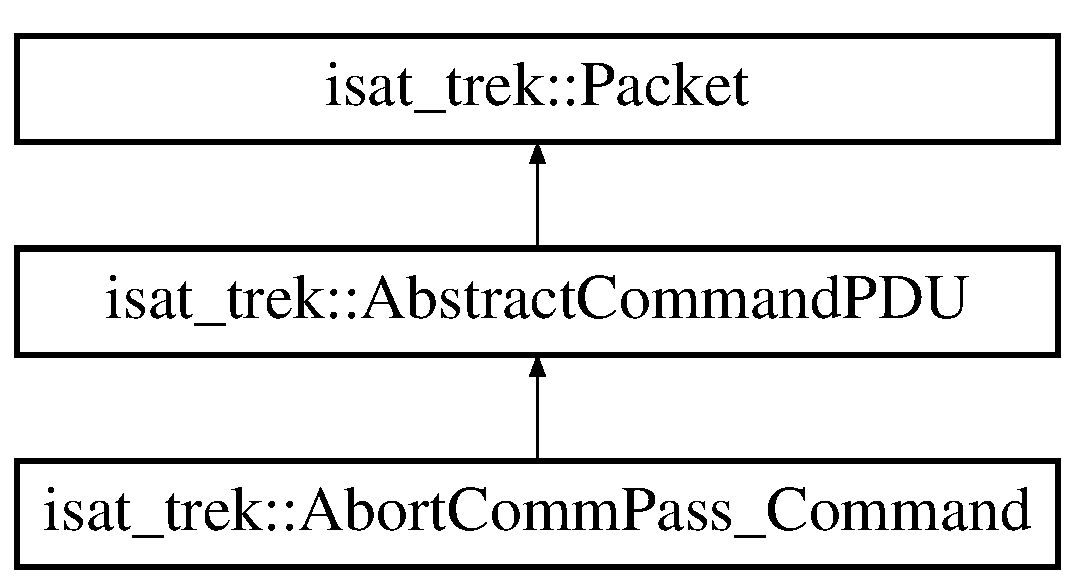
\includegraphics[height=3.000000cm]{classisat__trek_1_1_abort_comm_pass___command}
\end{center}
\end{figure}
\subsection*{Public Member Functions}
\begin{DoxyCompactItemize}
\item 
bool \hyperlink{classisat__trek_1_1_abort_comm_pass___command_ac7c845fe5a220a86c97515ed6c019fe1}{from\+Bytes} (Byte\+Buffer \&buf)
\item 
bool \hyperlink{classisat__trek_1_1_abort_comm_pass___command_a69a3b951da063672413e2ecbbc508dde}{to\+Bytes} (Byte\+Buffer \&buf)
\end{DoxyCompactItemize}
\subsection*{Additional Inherited Members}


\subsection{Detailed Description}
X\+XX\+: Replace with real description in isat.\+pdu file. 

\subsection{Member Function Documentation}
\index{isat\+\_\+trek\+::\+Abort\+Comm\+Pass\+\_\+\+Command@{isat\+\_\+trek\+::\+Abort\+Comm\+Pass\+\_\+\+Command}!from\+Bytes@{from\+Bytes}}
\index{from\+Bytes@{from\+Bytes}!isat\+\_\+trek\+::\+Abort\+Comm\+Pass\+\_\+\+Command@{isat\+\_\+trek\+::\+Abort\+Comm\+Pass\+\_\+\+Command}}
\subsubsection[{\texorpdfstring{from\+Bytes(\+Byte\+Buffer \&buf)}{fromBytes(ByteBuffer &buf)}}]{\setlength{\rightskip}{0pt plus 5cm}bool isat\+\_\+trek\+::\+Abort\+Comm\+Pass\+\_\+\+Command\+::from\+Bytes (
\begin{DoxyParamCaption}
\item[{Byte\+Buffer \&}]{buf}
\end{DoxyParamCaption}
)\hspace{0.3cm}{\ttfamily [virtual]}}\hypertarget{classisat__trek_1_1_abort_comm_pass___command_ac7c845fe5a220a86c97515ed6c019fe1}{}\label{classisat__trek_1_1_abort_comm_pass___command_ac7c845fe5a220a86c97515ed6c019fe1}
Populate the header and command fields from the data in buf.

\begin{DoxyReturn}{Returns}
true if successful. 
\end{DoxyReturn}


Implements \hyperlink{classisat__trek_1_1_packet}{isat\+\_\+trek\+::\+Packet}.

\index{isat\+\_\+trek\+::\+Abort\+Comm\+Pass\+\_\+\+Command@{isat\+\_\+trek\+::\+Abort\+Comm\+Pass\+\_\+\+Command}!to\+Bytes@{to\+Bytes}}
\index{to\+Bytes@{to\+Bytes}!isat\+\_\+trek\+::\+Abort\+Comm\+Pass\+\_\+\+Command@{isat\+\_\+trek\+::\+Abort\+Comm\+Pass\+\_\+\+Command}}
\subsubsection[{\texorpdfstring{to\+Bytes(\+Byte\+Buffer \&buf)}{toBytes(ByteBuffer &buf)}}]{\setlength{\rightskip}{0pt plus 5cm}bool isat\+\_\+trek\+::\+Abort\+Comm\+Pass\+\_\+\+Command\+::to\+Bytes (
\begin{DoxyParamCaption}
\item[{Byte\+Buffer \&}]{buf}
\end{DoxyParamCaption}
)\hspace{0.3cm}{\ttfamily [virtual]}}\hypertarget{classisat__trek_1_1_abort_comm_pass___command_a69a3b951da063672413e2ecbbc508dde}{}\label{classisat__trek_1_1_abort_comm_pass___command_a69a3b951da063672413e2ecbbc508dde}
Create the binary representation of this instance in the specified buffer.

\begin{DoxyReturn}{Returns}
true if successful. 
\end{DoxyReturn}


Implements \hyperlink{classisat__trek_1_1_packet}{isat\+\_\+trek\+::\+Packet}.



The documentation for this class was generated from the following files\+:\begin{DoxyCompactItemize}
\item 
/home/riley/work/fsw/src/isatgs/\+B\+A\+R\+Co\+Mm\+S/src/dependencies/trek/command/Abort\+Comm\+Pass\+\_\+\+Command.\+h\item 
/home/riley/work/fsw/src/isatgs/\+B\+A\+R\+Co\+Mm\+S/src/dependencies/trek/command/Abort\+Comm\+Pass\+\_\+\+Command.\+cpp\end{DoxyCompactItemize}

\hypertarget{classisat__trek_1_1_abstract_command_p_d_u}{}\section{isat\+\_\+trek\+:\+:Abstract\+Command\+P\+DU Class Reference}
\label{classisat__trek_1_1_abstract_command_p_d_u}\index{isat\+\_\+trek\+::\+Abstract\+Command\+P\+DU@{isat\+\_\+trek\+::\+Abstract\+Command\+P\+DU}}
Inheritance diagram for isat\+\_\+trek\+:\+:Abstract\+Command\+P\+DU\+:\begin{figure}[H]
\begin{center}
\leavevmode
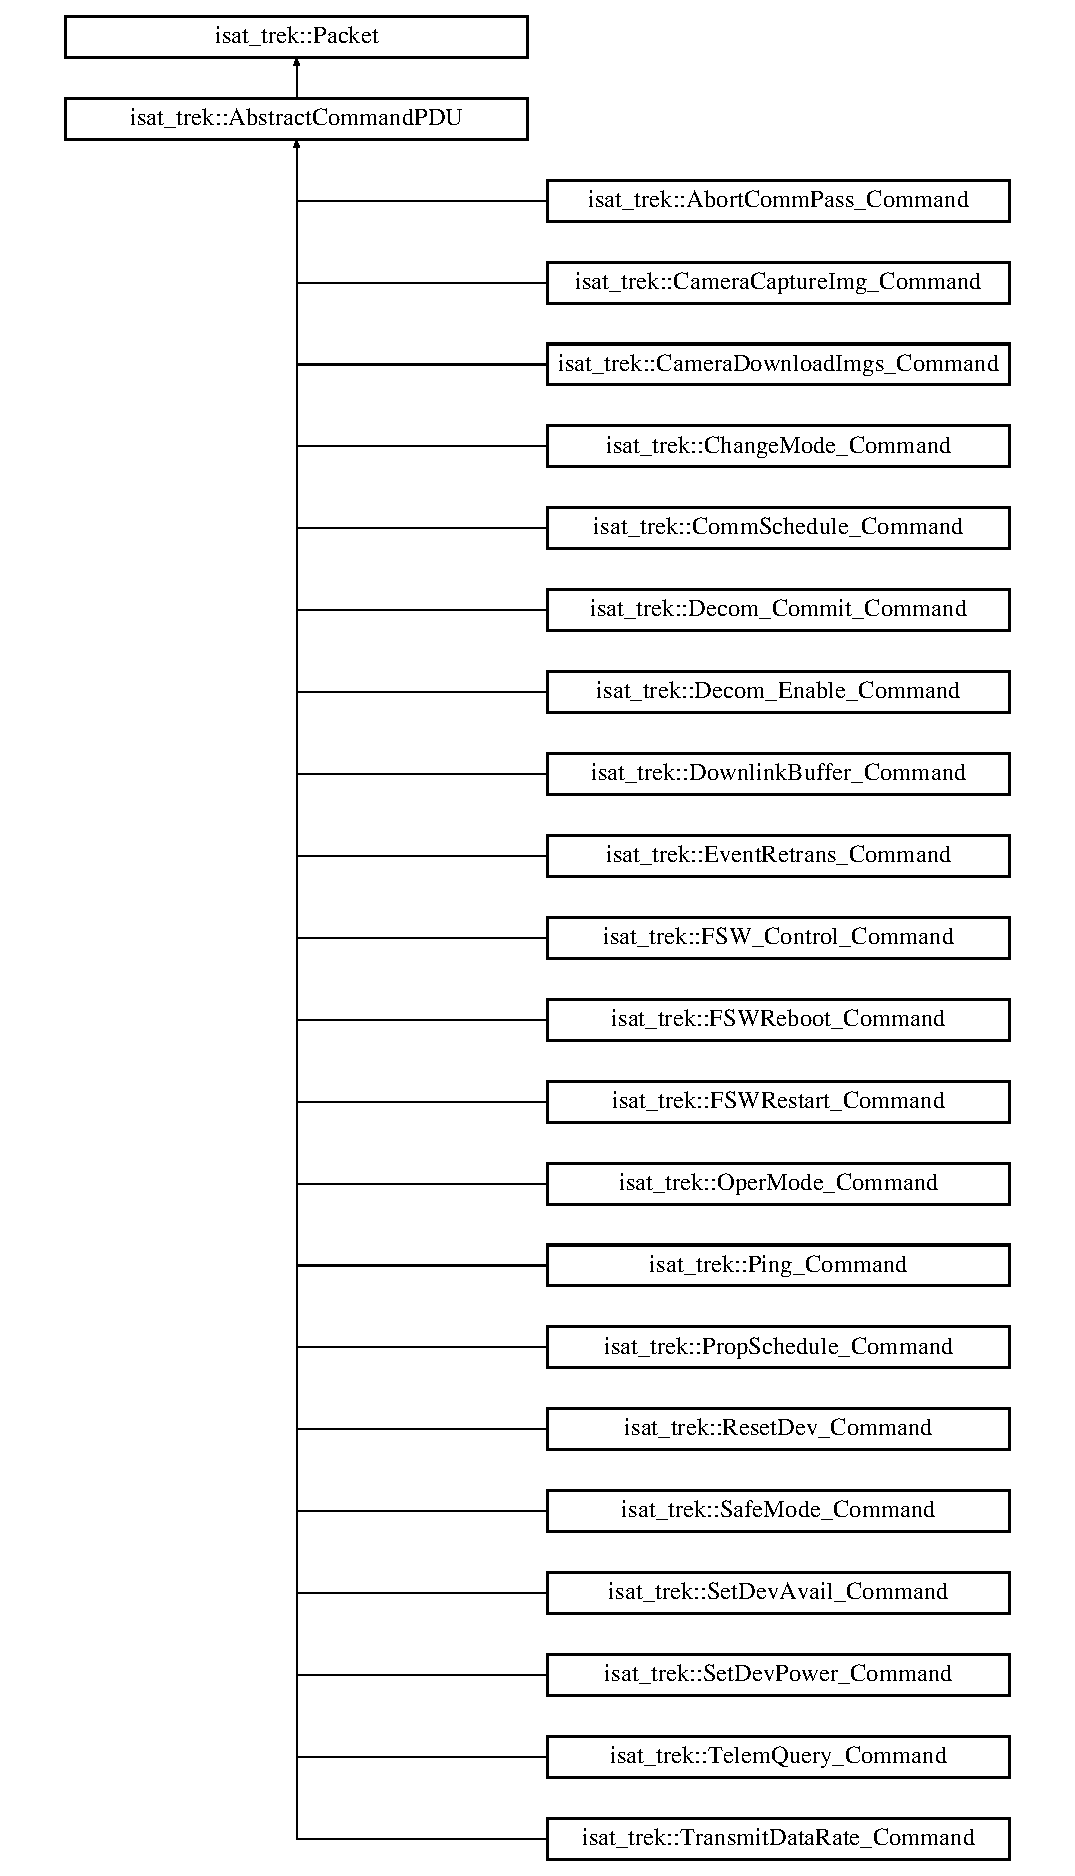
\includegraphics[height=12.000000cm]{classisat__trek_1_1_abstract_command_p_d_u}
\end{center}
\end{figure}
\subsection*{Public Member Functions}
\begin{DoxyCompactItemize}
\item 
int {\bfseries get\+A\+P\+ID} ()\hypertarget{classisat__trek_1_1_abstract_command_p_d_u_a48038919f3ee604341b6c855232afda4}{}\label{classisat__trek_1_1_abstract_command_p_d_u_a48038919f3ee604341b6c855232afda4}

\item 
int {\bfseries get\+Time\+Stamp} ()\hypertarget{classisat__trek_1_1_abstract_command_p_d_u_ad729263ce479b98139fc8015203ae862}{}\label{classisat__trek_1_1_abstract_command_p_d_u_ad729263ce479b98139fc8015203ae862}

\end{DoxyCompactItemize}
\subsection*{Public Attributes}
\begin{DoxyCompactItemize}
\item 
int {\bfseries V\+E\+R\+S\+I\+ON} = 0\hypertarget{classisat__trek_1_1_abstract_command_p_d_u_a75b7a1b245a92c6349c5d7eea9e9e1bd}{}\label{classisat__trek_1_1_abstract_command_p_d_u_a75b7a1b245a92c6349c5d7eea9e9e1bd}

\item 
int {\bfseries T\+Y\+PE} = 0\hypertarget{classisat__trek_1_1_abstract_command_p_d_u_a43c9d5f617cd57ae6231333a4cdb045c}{}\label{classisat__trek_1_1_abstract_command_p_d_u_a43c9d5f617cd57ae6231333a4cdb045c}

\item 
int {\bfseries S\+E\+C\+\_\+\+H\+D\+R\+\_\+\+F\+L\+AG} = 0\hypertarget{classisat__trek_1_1_abstract_command_p_d_u_a16943fbbdaf838b7dfb432d7d198ed8f}{}\label{classisat__trek_1_1_abstract_command_p_d_u_a16943fbbdaf838b7dfb432d7d198ed8f}

\item 
int {\bfseries A\+P\+ID}\hypertarget{classisat__trek_1_1_abstract_command_p_d_u_aef5543433dbaa870b2e8bc98b10085d2}{}\label{classisat__trek_1_1_abstract_command_p_d_u_aef5543433dbaa870b2e8bc98b10085d2}

\item 
int {\bfseries S\+E\+Q\+\_\+\+F\+L\+A\+GS} = 0\hypertarget{classisat__trek_1_1_abstract_command_p_d_u_a069f61f5f9b8683a11a5eda1bfc01267}{}\label{classisat__trek_1_1_abstract_command_p_d_u_a069f61f5f9b8683a11a5eda1bfc01267}

\item 
int {\bfseries P\+K\+T\+\_\+\+S\+E\+Q\+\_\+\+C\+O\+U\+NT} = 0\hypertarget{classisat__trek_1_1_abstract_command_p_d_u_a2847f7318b6466bd814ea730ef76a893}{}\label{classisat__trek_1_1_abstract_command_p_d_u_a2847f7318b6466bd814ea730ef76a893}

\item 
int {\bfseries P\+K\+T\+\_\+\+L\+E\+N\+G\+TH} = 0\hypertarget{classisat__trek_1_1_abstract_command_p_d_u_aa70736c8873284c966a521c52a77845c}{}\label{classisat__trek_1_1_abstract_command_p_d_u_aa70736c8873284c966a521c52a77845c}

\item 
int {\bfseries C\+O\+A\+R\+S\+E\+\_\+\+T\+I\+ME} = 0\hypertarget{classisat__trek_1_1_abstract_command_p_d_u_a458a6e92aab8fe487ca8751c2d412c42}{}\label{classisat__trek_1_1_abstract_command_p_d_u_a458a6e92aab8fe487ca8751c2d412c42}

\item 
int {\bfseries F\+I\+N\+E\+\_\+\+T\+I\+ME} = 0\hypertarget{classisat__trek_1_1_abstract_command_p_d_u_a366957cc9d9622136d29714b38ecafa1}{}\label{classisat__trek_1_1_abstract_command_p_d_u_a366957cc9d9622136d29714b38ecafa1}

\item 
int {\bfseries T\+I\+M\+E\+\_\+\+ID} = 0\hypertarget{classisat__trek_1_1_abstract_command_p_d_u_abdf50d2ab133a86f12cd3d833166f80f}{}\label{classisat__trek_1_1_abstract_command_p_d_u_abdf50d2ab133a86f12cd3d833166f80f}

\item 
int {\bfseries C\+H\+K\+W\+O\+R\+D\+\_\+\+I\+ND} = 0\hypertarget{classisat__trek_1_1_abstract_command_p_d_u_a0a2d2a0ab7f5eb766f20a9e0f77400a0}{}\label{classisat__trek_1_1_abstract_command_p_d_u_a0a2d2a0ab7f5eb766f20a9e0f77400a0}

\item 
int {\bfseries Z\+OE} = 0\hypertarget{classisat__trek_1_1_abstract_command_p_d_u_ab442065d36e0f148c419463bc13fa0c8}{}\label{classisat__trek_1_1_abstract_command_p_d_u_ab442065d36e0f148c419463bc13fa0c8}

\item 
int {\bfseries P\+K\+T\+\_\+\+T\+Y\+PE} = 0\hypertarget{classisat__trek_1_1_abstract_command_p_d_u_a435a78f8789c7d53c193ca92927d2183}{}\label{classisat__trek_1_1_abstract_command_p_d_u_a435a78f8789c7d53c193ca92927d2183}

\item 
int {\bfseries S\+P\+A\+R\+E1} = 0\hypertarget{classisat__trek_1_1_abstract_command_p_d_u_a946d7209bffcf3130ae5587ce2bede78}{}\label{classisat__trek_1_1_abstract_command_p_d_u_a946d7209bffcf3130ae5587ce2bede78}

\item 
int {\bfseries E\+L\+E\+M\+E\+N\+T\+\_\+\+ID} = 0\hypertarget{classisat__trek_1_1_abstract_command_p_d_u_a12be31177eab91e81ad9b21741d5fb4e}{}\label{classisat__trek_1_1_abstract_command_p_d_u_a12be31177eab91e81ad9b21741d5fb4e}

\item 
int {\bfseries C\+M\+D\+\_\+\+P\+A\+C\+K\+ET} = 0\hypertarget{classisat__trek_1_1_abstract_command_p_d_u_a875ab55f9df6d2cdeb56a4d9db5a7380}{}\label{classisat__trek_1_1_abstract_command_p_d_u_a875ab55f9df6d2cdeb56a4d9db5a7380}

\item 
int {\bfseries S\+P\+A\+R\+E2} = 0\hypertarget{classisat__trek_1_1_abstract_command_p_d_u_a159420f7e762317b6e340ad08824b030}{}\label{classisat__trek_1_1_abstract_command_p_d_u_a159420f7e762317b6e340ad08824b030}

\item 
int {\bfseries L\+D\+P\+\_\+\+E\+N\+D\+P\+O\+I\+NT}\hypertarget{classisat__trek_1_1_abstract_command_p_d_u_a613a9b40729913785ae3e0ec78b994e7}{}\label{classisat__trek_1_1_abstract_command_p_d_u_a613a9b40729913785ae3e0ec78b994e7}

\item 
int {\bfseries S\+U\+B\+S\+E\+T\+\_\+\+ID} = 0\hypertarget{classisat__trek_1_1_abstract_command_p_d_u_a562f4c11df5603e18ced9870d99c60ba}{}\label{classisat__trek_1_1_abstract_command_p_d_u_a562f4c11df5603e18ced9870d99c60ba}

\item 
int {\bfseries S\+P\+A\+R\+E3} = 0\hypertarget{classisat__trek_1_1_abstract_command_p_d_u_a98d45cf4066b501e101487e9dad7fb14}{}\label{classisat__trek_1_1_abstract_command_p_d_u_a98d45cf4066b501e101487e9dad7fb14}

\item 
int {\bfseries L\+E\+G\+A\+L\+\_\+\+M\+O\+D\+ES} = 0\hypertarget{classisat__trek_1_1_abstract_command_p_d_u_a35ceaaa29261e315e3ae291221d42ff9}{}\label{classisat__trek_1_1_abstract_command_p_d_u_a35ceaaa29261e315e3ae291221d42ff9}

\end{DoxyCompactItemize}


The documentation for this class was generated from the following file\+:\begin{DoxyCompactItemize}
\item 
/home/riley/work/fsw/src/isatgs/\+B\+A\+R\+Co\+Mm\+S/src/dependencies/trek/Abstract\+Command\+P\+D\+U.\+h\end{DoxyCompactItemize}

\hypertarget{classisat__trek_1_1_abstract_telemetry_p_d_u}{}\section{isat\+\_\+trek\+:\+:Abstract\+Telemetry\+P\+DU Class Reference}
\label{classisat__trek_1_1_abstract_telemetry_p_d_u}\index{isat\+\_\+trek\+::\+Abstract\+Telemetry\+P\+DU@{isat\+\_\+trek\+::\+Abstract\+Telemetry\+P\+DU}}
Inheritance diagram for isat\+\_\+trek\+:\+:Abstract\+Telemetry\+P\+DU\+:\begin{figure}[H]
\begin{center}
\leavevmode
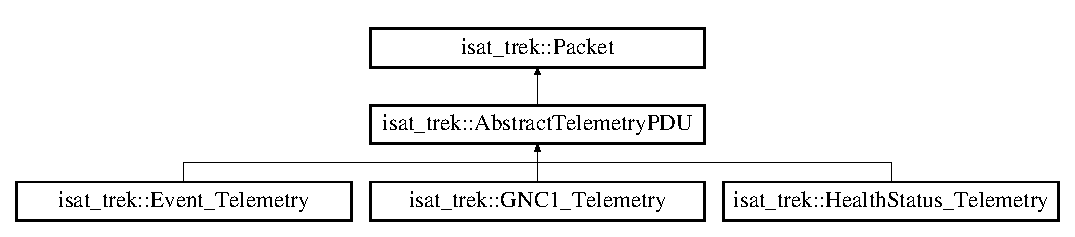
\includegraphics[height=2.731707cm]{classisat__trek_1_1_abstract_telemetry_p_d_u}
\end{center}
\end{figure}
\subsection*{Public Attributes}
\begin{DoxyCompactItemize}
\item 
int16\+\_\+t {\bfseries apid}\hypertarget{classisat__trek_1_1_abstract_telemetry_p_d_u_a8d68fb30bcce86339235a3a14b72f041}{}\label{classisat__trek_1_1_abstract_telemetry_p_d_u_a8d68fb30bcce86339235a3a14b72f041}

\item 
int64\+\_\+t {\bfseries time}\hypertarget{classisat__trek_1_1_abstract_telemetry_p_d_u_affa9a64e7a5f63f83ce6d81f3e8e525f}{}\label{classisat__trek_1_1_abstract_telemetry_p_d_u_affa9a64e7a5f63f83ce6d81f3e8e525f}

\item 
int32\+\_\+t {\bfseries object\+Id}\hypertarget{classisat__trek_1_1_abstract_telemetry_p_d_u_a4cc65c6b3adf09479794bb66ba71da22}{}\label{classisat__trek_1_1_abstract_telemetry_p_d_u_a4cc65c6b3adf09479794bb66ba71da22}

\end{DoxyCompactItemize}
\subsection*{Additional Inherited Members}


The documentation for this class was generated from the following file\+:\begin{DoxyCompactItemize}
\item 
/home/riley/work/fsw/src/isatgs/\+B\+A\+R\+Co\+Mm\+S/src/dependencies/trek/Abstract\+Telemetry\+P\+D\+U.\+h\end{DoxyCompactItemize}

\hypertarget{struct_a_c_k}{}\section{A\+CK Struct Reference}
\label{struct_a_c_k}\index{A\+CK@{A\+CK}}
\subsection*{Public Attributes}
\begin{DoxyCompactItemize}
\item 
u\+\_\+int\+\_\+1 {\bfseries directive\+\_\+code}\+: 4\hypertarget{struct_a_c_k_a9d1bc82f590c27eb334b3edaf0beaf25}{}\label{struct_a_c_k_a9d1bc82f590c27eb334b3edaf0beaf25}

\item 
u\+\_\+int\+\_\+1 {\bfseries directive\+\_\+subtype\+\_\+code}\+: 4\hypertarget{struct_a_c_k_a5d377c03910335c534b288ae9d516cc0}{}\label{struct_a_c_k_a5d377c03910335c534b288ae9d516cc0}

\item 
u\+\_\+int\+\_\+1 {\bfseries condition\+\_\+code}\+: 4\hypertarget{struct_a_c_k_a88a6885f40b72b90ff9016a9e69deb10}{}\label{struct_a_c_k_a88a6885f40b72b90ff9016a9e69deb10}

\item 
u\+\_\+int\+\_\+1 {\bfseries delivery\+\_\+code}\+: 2\hypertarget{struct_a_c_k_ae4cfa1794f86a137a440b43558873a42}{}\label{struct_a_c_k_ae4cfa1794f86a137a440b43558873a42}

\item 
u\+\_\+int\+\_\+1 {\bfseries transaction\+\_\+status}\+: 2\hypertarget{struct_a_c_k_a23f71d78a642ee940d522f1fba8d65c6}{}\label{struct_a_c_k_a23f71d78a642ee940d522f1fba8d65c6}

\end{DoxyCompactItemize}


The documentation for this struct was generated from the following file\+:\begin{DoxyCompactItemize}
\item 
/home/riley/work/fsw/src/isatgs/\+B\+A\+R\+Co\+Mm\+S/src/dependencies/\+C\+F\+D\+P/\+P\+R\+I/structures.\+h\end{DoxyCompactItemize}

\hypertarget{classisat__utils_1_1_array_list}{}\section{isat\+\_\+utils\+:\+:Array\+List$<$ T $>$ Class Template Reference}
\label{classisat__utils_1_1_array_list}\index{isat\+\_\+utils\+::\+Array\+List$<$ T $>$@{isat\+\_\+utils\+::\+Array\+List$<$ T $>$}}


{\ttfamily \#include $<$Array\+List.\+h$>$}

\subsection*{Public Member Functions}
\begin{DoxyCompactItemize}
\item 
{\bfseries Array\+List} (int max\+Size=100)\hypertarget{classisat__utils_1_1_array_list_a047dfeb4558a3c00f4a7869e483e5560}{}\label{classisat__utils_1_1_array_list_a047dfeb4558a3c00f4a7869e483e5560}

\item 
{\bfseries Array\+List} (\hyperlink{classisat__utils_1_1_array_list}{Array\+List}$<$ T $>$ const \&rhs)\hypertarget{classisat__utils_1_1_array_list_aadad63e6e7467804583692241e48e7f3}{}\label{classisat__utils_1_1_array_list_aadad63e6e7467804583692241e48e7f3}

\item 
\hyperlink{classisat__utils_1_1_array_list}{Array\+List}$<$ T $>$ \& {\bfseries operator=} (\hyperlink{classisat__utils_1_1_array_list}{Array\+List}$<$ T $>$ \&rhs)\hypertarget{classisat__utils_1_1_array_list_a181b240f65d9070a2481899aaced9041}{}\label{classisat__utils_1_1_array_list_a181b240f65d9070a2481899aaced9041}

\item 
bool {\bfseries error} ()\hypertarget{classisat__utils_1_1_array_list_a4030036863ef8b6b91b5081aa55dbddd}{}\label{classisat__utils_1_1_array_list_a4030036863ef8b6b91b5081aa55dbddd}

\item 
void {\bfseries clear} ()\hypertarget{classisat__utils_1_1_array_list_a94ef082dc86abf943a4f4d37ad7df655}{}\label{classisat__utils_1_1_array_list_a94ef082dc86abf943a4f4d37ad7df655}

\item 
bool {\bfseries add} (T element)\hypertarget{classisat__utils_1_1_array_list_aa8bc6b5d62c88f7d578e8ffd2cd203d6}{}\label{classisat__utils_1_1_array_list_aa8bc6b5d62c88f7d578e8ffd2cd203d6}

\item 
bool \hyperlink{classisat__utils_1_1_array_list_abfaa096b1e41b8463f7e034c8ba40ae2}{put} (int index, T element)
\item 
bool {\bfseries contains} (T element)\hypertarget{classisat__utils_1_1_array_list_a93c3ba50cd56aef241f149a3ee74b95b}{}\label{classisat__utils_1_1_array_list_a93c3ba50cd56aef241f149a3ee74b95b}

\item 
bool {\bfseries get} (int index, T \&element) const \hypertarget{classisat__utils_1_1_array_list_a81fe1bd3a585fde32eafd67d5f113787}{}\label{classisat__utils_1_1_array_list_a81fe1bd3a585fde32eafd67d5f113787}

\item 
bool {\bfseries index\+Of} (T element, int \&index) const \hypertarget{classisat__utils_1_1_array_list_a06dd0e867e93b0be5c28038d15a76545}{}\label{classisat__utils_1_1_array_list_a06dd0e867e93b0be5c28038d15a76545}

\item 
bool {\bfseries is\+Empty} ()\hypertarget{classisat__utils_1_1_array_list_adbaef89ffb6e2659040aab3933284cea}{}\label{classisat__utils_1_1_array_list_adbaef89ffb6e2659040aab3933284cea}

\item 
bool {\bfseries remove} (int index)\hypertarget{classisat__utils_1_1_array_list_ab6e75564e4912810d54d20f9c6e6827c}{}\label{classisat__utils_1_1_array_list_ab6e75564e4912810d54d20f9c6e6827c}

\item 
bool {\bfseries remove\+Element} (T element)\hypertarget{classisat__utils_1_1_array_list_a197be365458a7812aaa0a69f09d13c1b}{}\label{classisat__utils_1_1_array_list_a197be365458a7812aaa0a69f09d13c1b}

\item 
bool {\bfseries set} (int index, T element)\hypertarget{classisat__utils_1_1_array_list_a5007800ae33650919dd11f4a23296178}{}\label{classisat__utils_1_1_array_list_a5007800ae33650919dd11f4a23296178}

\item 
int {\bfseries size} () const \hypertarget{classisat__utils_1_1_array_list_a5edf6973d1b2d71267a2fb8097879862}{}\label{classisat__utils_1_1_array_list_a5edf6973d1b2d71267a2fb8097879862}

\item 
int {\bfseries capacity} () const \hypertarget{classisat__utils_1_1_array_list_acf7ae0900bdba81e539c37c990ff5714}{}\label{classisat__utils_1_1_array_list_acf7ae0900bdba81e539c37c990ff5714}

\end{DoxyCompactItemize}


\subsection{Detailed Description}
\subsubsection*{template$<$class T$>$\\*
class isat\+\_\+utils\+::\+Array\+List$<$ T $>$}

Exception safe version of a simple list container. Modeled after java\textquotesingle{}s \hyperlink{classisat__utils_1_1_array_list}{Array\+List}.

Unlike std\+::vector, An \hyperlink{classisat__utils_1_1_array_list}{Array\+List} instance\textquotesingle{}s size is fixed when created. The number of elements in the list may change (the \textquotesingle{}size\textquotesingle{}) but the capacity never changes.

Note that because it\textquotesingle{}s \char`\"{}exception safe\char`\"{} (throws no exceptions), certain compromises in ease of use had to be made. Often, the natural way to do a particular thing (return a value) leaves no room for an error code (other than an exception). If the interface seems awkward in places, this is why. 

\subsection{Member Function Documentation}
\index{isat\+\_\+utils\+::\+Array\+List@{isat\+\_\+utils\+::\+Array\+List}!put@{put}}
\index{put@{put}!isat\+\_\+utils\+::\+Array\+List@{isat\+\_\+utils\+::\+Array\+List}}
\subsubsection[{\texorpdfstring{put(int index, T element)}{put(int index, T element)}}]{\setlength{\rightskip}{0pt plus 5cm}template$<$class T$>$ bool {\bf isat\+\_\+utils\+::\+Array\+List}$<$ T $>$\+::put (
\begin{DoxyParamCaption}
\item[{int}]{index, }
\item[{T}]{element}
\end{DoxyParamCaption}
)}\hypertarget{classisat__utils_1_1_array_list_abfaa096b1e41b8463f7e034c8ba40ae2}{}\label{classisat__utils_1_1_array_list_abfaa096b1e41b8463f7e034c8ba40ae2}
Insert element in 

The documentation for this class was generated from the following file\+:\begin{DoxyCompactItemize}
\item 
/home/riley/work/fsw/src/isatgs/\+B\+A\+R\+Co\+Mm\+S/src/dependencies/utils/Array\+List.\+h\end{DoxyCompactItemize}

\hypertarget{class_b_a_r_co_mm_s___camera}{}\section{B\+A\+R\+Co\+Mm\+S\+\_\+\+Camera Class Reference}
\label{class_b_a_r_co_mm_s___camera}\index{B\+A\+R\+Co\+Mm\+S\+\_\+\+Camera@{B\+A\+R\+Co\+Mm\+S\+\_\+\+Camera}}
Inheritance diagram for B\+A\+R\+Co\+Mm\+S\+\_\+\+Camera\+:\begin{figure}[H]
\begin{center}
\leavevmode
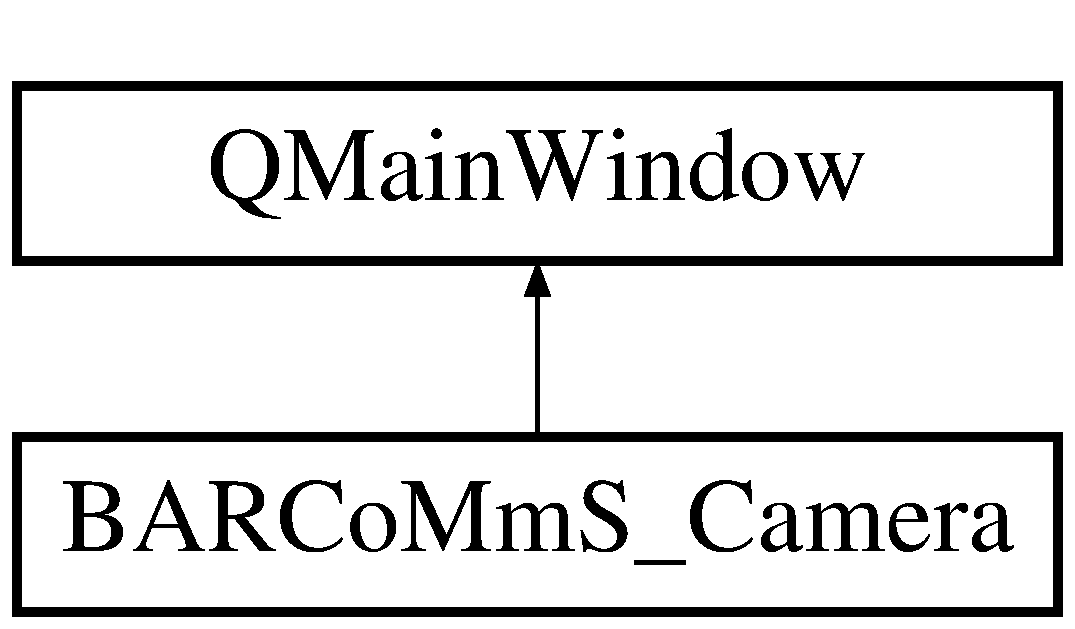
\includegraphics[height=2.000000cm]{class_b_a_r_co_mm_s___camera}
\end{center}
\end{figure}
\subsection*{Public Member Functions}
\begin{DoxyCompactItemize}
\item 
{\bfseries B\+A\+R\+Co\+Mm\+S\+\_\+\+Camera} (Q\+Widget $\ast$parent=0)\hypertarget{class_b_a_r_co_mm_s___camera_a82305edb0c24e3a15520e592fb09d322}{}\label{class_b_a_r_co_mm_s___camera_a82305edb0c24e3a15520e592fb09d322}

\item 
void {\bfseries close\+Event} (Q\+Close\+Event $\ast$event)\hypertarget{class_b_a_r_co_mm_s___camera_a50fddeb61c65a113a47961ab657f39ea}{}\label{class_b_a_r_co_mm_s___camera_a50fddeb61c65a113a47961ab657f39ea}

\item 
void {\bfseries initialize\+Image\+List} (const Q\+String \&path)\hypertarget{class_b_a_r_co_mm_s___camera_a74572bf6c446ca33767f04937d8cb709}{}\label{class_b_a_r_co_mm_s___camera_a74572bf6c446ca33767f04937d8cb709}

\end{DoxyCompactItemize}
\subsection*{Public Attributes}
\begin{DoxyCompactItemize}
\item 
Ui\+::\+B\+A\+R\+Co\+Mm\+S\+\_\+\+Camera $\ast$ {\bfseries ui}\hypertarget{class_b_a_r_co_mm_s___camera_aa2f9a4b998e1f397e49528d4e8e7173b}{}\label{class_b_a_r_co_mm_s___camera_aa2f9a4b998e1f397e49528d4e8e7173b}

\item 
Q\+Pixmap {\bfseries image}\hypertarget{class_b_a_r_co_mm_s___camera_aa8f7f1b9f8e04e7f92a990922b60dc1e}{}\label{class_b_a_r_co_mm_s___camera_aa8f7f1b9f8e04e7f92a990922b60dc1e}

\item 
Q\+Image $\ast$ {\bfseries image\+Object}\hypertarget{class_b_a_r_co_mm_s___camera_a9d150cf6177ec17f84a3d7ed162d3ff2}{}\label{class_b_a_r_co_mm_s___camera_a9d150cf6177ec17f84a3d7ed162d3ff2}

\item 
G\+Luint $\ast$ {\bfseries tex}\hypertarget{class_b_a_r_co_mm_s___camera_aad43c7098f0dca2265ffc64a55933301}{}\label{class_b_a_r_co_mm_s___camera_aad43c7098f0dca2265ffc64a55933301}

\item 
Q\+String $\ast$ {\bfseries i\+Path}\hypertarget{class_b_a_r_co_mm_s___camera_aaff4ee3780e3207d86d3346f49148f54}{}\label{class_b_a_r_co_mm_s___camera_aaff4ee3780e3207d86d3346f49148f54}

\item 
Q\+File\+System\+Watcher $\ast$ {\bfseries watcher}\hypertarget{class_b_a_r_co_mm_s___camera_aa02730f8b4ed1e9621cfa879d0aebb5f}{}\label{class_b_a_r_co_mm_s___camera_aa02730f8b4ed1e9621cfa879d0aebb5f}

\item 
Q\+Time $\ast$ {\bfseries past\+Time}\hypertarget{class_b_a_r_co_mm_s___camera_a6336d6842085bfea47e96949c6c5c7b6}{}\label{class_b_a_r_co_mm_s___camera_a6336d6842085bfea47e96949c6c5c7b6}

\item 
Q\+Vector$<$ Q\+String $>$ {\bfseries image\+List}\hypertarget{class_b_a_r_co_mm_s___camera_a4f6a81ccec89d9d3696dbce8d700653e}{}\label{class_b_a_r_co_mm_s___camera_a4f6a81ccec89d9d3696dbce8d700653e}

\item 
int {\bfseries image\+List\+Size}\hypertarget{class_b_a_r_co_mm_s___camera_a61c474d5de45504f0c6dcd31ff531e93}{}\label{class_b_a_r_co_mm_s___camera_a61c474d5de45504f0c6dcd31ff531e93}

\end{DoxyCompactItemize}


The documentation for this class was generated from the following files\+:\begin{DoxyCompactItemize}
\item 
/home/riley/work/fsw/src/isatgs/\+B\+A\+R\+Co\+Mm\+S/src/modules/\+B\+A\+R\+Co\+Mm\+S\+\_\+\+Camera/barcomms\+\_\+camera.\+h\item 
/home/riley/work/fsw/src/isatgs/\+B\+A\+R\+Co\+Mm\+S/src/modules/\+B\+A\+R\+Co\+Mm\+S\+\_\+\+Camera/barcomms\+\_\+camera.\+cpp\end{DoxyCompactItemize}

\hypertarget{class_b_a_r_co_mm_s___c_f_d_p}{}\section{B\+A\+R\+Co\+Mm\+S\+\_\+\+C\+F\+DP Class Reference}
\label{class_b_a_r_co_mm_s___c_f_d_p}\index{B\+A\+R\+Co\+Mm\+S\+\_\+\+C\+F\+DP@{B\+A\+R\+Co\+Mm\+S\+\_\+\+C\+F\+DP}}
Inheritance diagram for B\+A\+R\+Co\+Mm\+S\+\_\+\+C\+F\+DP\+:\begin{figure}[H]
\begin{center}
\leavevmode
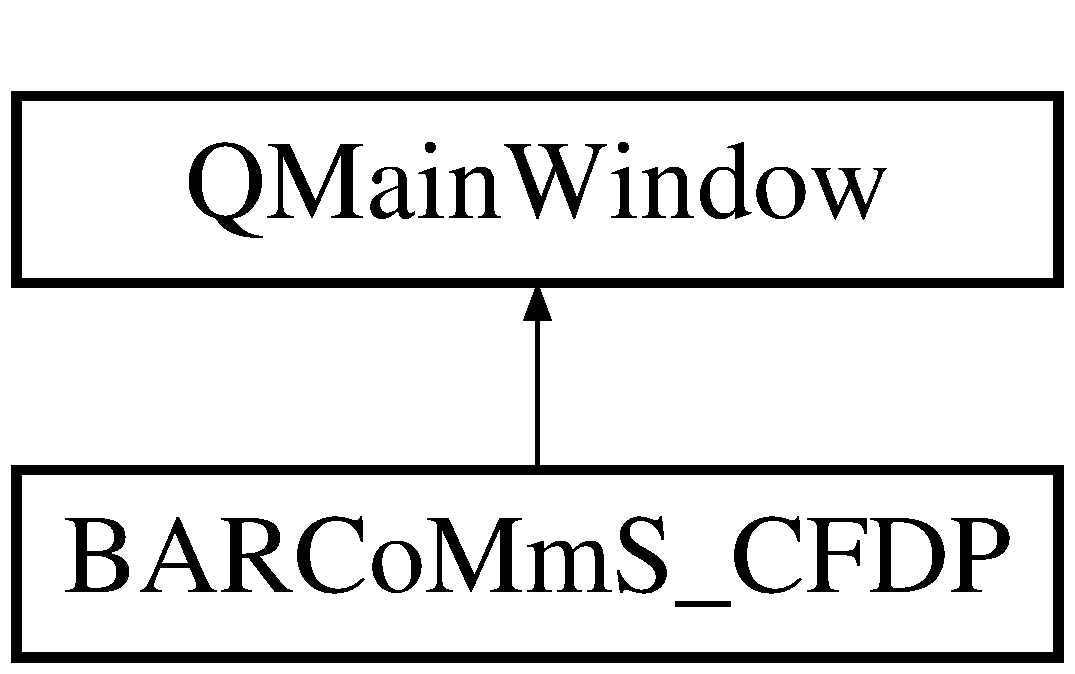
\includegraphics[height=2.000000cm]{class_b_a_r_co_mm_s___c_f_d_p}
\end{center}
\end{figure}
\subsection*{Signals}
\begin{DoxyCompactItemize}
\item 
void {\bfseries to\+Bulletin} (char $\ast$)\hypertarget{class_b_a_r_co_mm_s___c_f_d_p_a975b37b480250f8b8b7c38264b821283}{}\label{class_b_a_r_co_mm_s___c_f_d_p_a975b37b480250f8b8b7c38264b821283}

\item 
void {\bfseries terminator} ()\hypertarget{class_b_a_r_co_mm_s___c_f_d_p_acf41dbaeaa1587919298d11e1d2030b8}{}\label{class_b_a_r_co_mm_s___c_f_d_p_acf41dbaeaa1587919298d11e1d2030b8}

\end{DoxyCompactItemize}
\subsection*{Public Member Functions}
\begin{DoxyCompactItemize}
\item 
{\bfseries B\+A\+R\+Co\+Mm\+S\+\_\+\+C\+F\+DP} (Q\+Widget $\ast$parent=0)\hypertarget{class_b_a_r_co_mm_s___c_f_d_p_a7b019e2adc1c17e4dcf74d71ec493454}{}\label{class_b_a_r_co_mm_s___c_f_d_p_a7b019e2adc1c17e4dcf74d71ec493454}

\item 
void {\bfseries close\+Event} (Q\+Close\+Event $\ast$event)\hypertarget{class_b_a_r_co_mm_s___c_f_d_p_ad1562e35303a406ca01e5224dffa051f}{}\label{class_b_a_r_co_mm_s___c_f_d_p_ad1562e35303a406ca01e5224dffa051f}

\end{DoxyCompactItemize}


The documentation for this class was generated from the following files\+:\begin{DoxyCompactItemize}
\item 
/home/riley/work/fsw/src/isatgs/\+B\+A\+R\+Co\+Mm\+S/src/modules/\+B\+A\+R\+Co\+Mm\+S\+\_\+\+C\+F\+D\+P/barcomms\+\_\+cfdp.\+h\item 
/home/riley/work/fsw/src/isatgs/\+B\+A\+R\+Co\+Mm\+S/src/modules/\+B\+A\+R\+Co\+Mm\+S\+\_\+\+C\+F\+D\+P/barcomms\+\_\+cfdp.\+cpp\end{DoxyCompactItemize}

\hypertarget{class_b_c___bulletin}{}\section{B\+C\+\_\+\+Bulletin Class Reference}
\label{class_b_c___bulletin}\index{B\+C\+\_\+\+Bulletin@{B\+C\+\_\+\+Bulletin}}
Inheritance diagram for B\+C\+\_\+\+Bulletin\+:\begin{figure}[H]
\begin{center}
\leavevmode
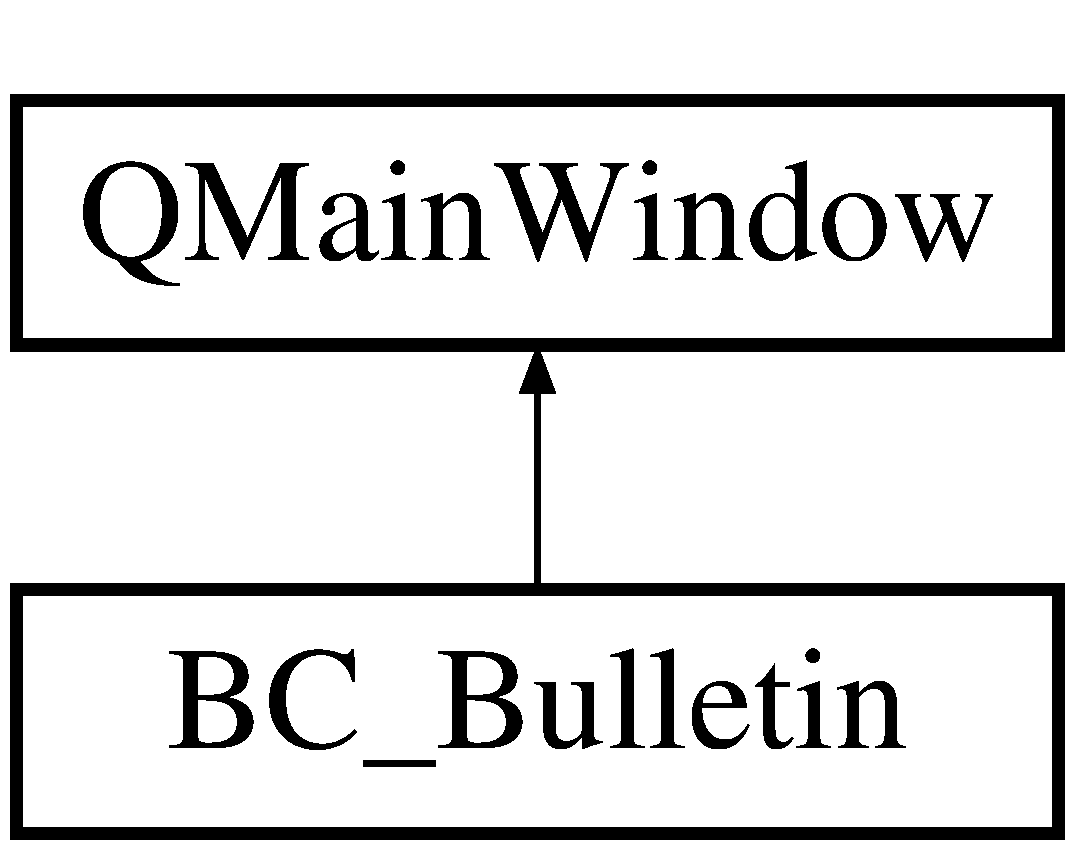
\includegraphics[height=2.000000cm]{class_b_c___bulletin}
\end{center}
\end{figure}
\subsection*{Public Slots}
\begin{DoxyCompactItemize}
\item 
void {\bfseries take\+C\+F\+DP} (char $\ast$str)\hypertarget{class_b_c___bulletin_a4babf972dd93fd4e34e6dcf29eb48b3d}{}\label{class_b_c___bulletin_a4babf972dd93fd4e34e6dcf29eb48b3d}

\item 
void {\bfseries take\+F\+SW} (int apid, int id)\hypertarget{class_b_c___bulletin_a8fcb6574f3d2f24eff6ea417ef24c45d}{}\label{class_b_c___bulletin_a8fcb6574f3d2f24eff6ea417ef24c45d}

\item 
void {\bfseries pdu\+Received} (Byte\+Buffer)\hypertarget{class_b_c___bulletin_a551dcc00416dc798c4e46a25095fe190}{}\label{class_b_c___bulletin_a551dcc00416dc798c4e46a25095fe190}

\item 
void {\bfseries go\+To} ()\hypertarget{class_b_c___bulletin_a523b71bcbdfe705977b1619cdb6829ac}{}\label{class_b_c___bulletin_a523b71bcbdfe705977b1619cdb6829ac}

\item 
void {\bfseries erase\+Search\+Bar} ()\hypertarget{class_b_c___bulletin_ae5080fd90559453a3ecf9d0246403da4}{}\label{class_b_c___bulletin_ae5080fd90559453a3ecf9d0246403da4}

\item 
void {\bfseries expand\+Collapse\+Item} ()\hypertarget{class_b_c___bulletin_a4245fd8227d9cd9e5b94a3ed56c73e20}{}\label{class_b_c___bulletin_a4245fd8227d9cd9e5b94a3ed56c73e20}

\item 
void {\bfseries expand\+Collapse\+All} ()\hypertarget{class_b_c___bulletin_a6350f7ee846b9cf45eb4bb6033da4447}{}\label{class_b_c___bulletin_a6350f7ee846b9cf45eb4bb6033da4447}

\item 
void {\bfseries auto\+Scroll} ()\hypertarget{class_b_c___bulletin_a289ebaa508a386be0e9d4d0ad2c05aa8}{}\label{class_b_c___bulletin_a289ebaa508a386be0e9d4d0ad2c05aa8}

\item 
void {\bfseries auto\+Expand} ()\hypertarget{class_b_c___bulletin_ae1248ce04f5cdfceece188dd1c0695f9}{}\label{class_b_c___bulletin_ae1248ce04f5cdfceece188dd1c0695f9}

\item 
void {\bfseries open\+Sorting} ()\hypertarget{class_b_c___bulletin_ade59035454b840aa2875c45522eecc1c}{}\label{class_b_c___bulletin_ade59035454b840aa2875c45522eecc1c}

\item 
void {\bfseries sort\+Items} (int sort\+Option)\hypertarget{class_b_c___bulletin_a8cb5af84080851cdb1aa58145b454f54}{}\label{class_b_c___bulletin_a8cb5af84080851cdb1aa58145b454f54}

\end{DoxyCompactItemize}
\subsection*{Signals}
\begin{DoxyCompactItemize}
\item 
void {\bfseries rssi} (int)\hypertarget{class_b_c___bulletin_a1d5d9d5d4ff0f3c92c3ecc1984710961}{}\label{class_b_c___bulletin_a1d5d9d5d4ff0f3c92c3ecc1984710961}

\item 
void {\bfseries item\+Added} ()\hypertarget{class_b_c___bulletin_a45931b7da29f76b4ffe08828d1d81580}{}\label{class_b_c___bulletin_a45931b7da29f76b4ffe08828d1d81580}

\item 
void {\bfseries dying} ()\hypertarget{class_b_c___bulletin_a560ed1f975f659188cdc4c98f5f96773}{}\label{class_b_c___bulletin_a560ed1f975f659188cdc4c98f5f96773}

\end{DoxyCompactItemize}
\subsection*{Public Member Functions}
\begin{DoxyCompactItemize}
\item 
{\bfseries B\+C\+\_\+\+Bulletin} (Q\+Widget $\ast$parent=0)\hypertarget{class_b_c___bulletin_a41ae9ac01a108f7bf4b6aba315d5e4b0}{}\label{class_b_c___bulletin_a41ae9ac01a108f7bf4b6aba315d5e4b0}

\item 
void {\bfseries remove\+Items} (int tree)\hypertarget{class_b_c___bulletin_ac82707f3d09a5e14d9f33564e751f05b}{}\label{class_b_c___bulletin_ac82707f3d09a5e14d9f33564e751f05b}

\item 
void {\bfseries replace\+Items} (int tree)\hypertarget{class_b_c___bulletin_a2a473cbef765f03ff0a2d60b434cd06b}{}\label{class_b_c___bulletin_a2a473cbef765f03ff0a2d60b434cd06b}

\item 
void {\bfseries close\+Event} (Q\+Close\+Event $\ast$)\hypertarget{class_b_c___bulletin_a7d8e89a713031ae32986c1fa6a05ee44}{}\label{class_b_c___bulletin_a7d8e89a713031ae32986c1fa6a05ee44}

\end{DoxyCompactItemize}
\subsection*{Public Attributes}
\begin{DoxyCompactItemize}
\item 
Q\+String {\bfseries last\+Num}\hypertarget{class_b_c___bulletin_a02b94a8421b4d9d5a0fa67ad4163c589}{}\label{class_b_c___bulletin_a02b94a8421b4d9d5a0fa67ad4163c589}

\item 
Q\+List$<$ \hyperlink{class_item}{Item} $>$ {\bfseries tree\+Items}\hypertarget{class_b_c___bulletin_a684dee5e9518c21f74f517fab9044eb3}{}\label{class_b_c___bulletin_a684dee5e9518c21f74f517fab9044eb3}

\item 
Q\+List$<$ \hyperlink{class_f_s_w_item}{F\+S\+W\+Item} $\ast$ $>$ {\bfseries fsw\+Tree\+Items}\hypertarget{class_b_c___bulletin_a635d32b92a3e61555613119c3282478e}{}\label{class_b_c___bulletin_a635d32b92a3e61555613119c3282478e}

\item 
Q\+Color {\bfseries red} = Q\+Color(255, 85, 85, 160)\hypertarget{class_b_c___bulletin_a3ac5f0b6fda0e8f5fd16b12563c4dfd8}{}\label{class_b_c___bulletin_a3ac5f0b6fda0e8f5fd16b12563c4dfd8}

\item 
Q\+Color {\bfseries orange} = Q\+Color(255, 154, 53, 145)\hypertarget{class_b_c___bulletin_a89ea24b766d8fb3b160756156b78d3d3}{}\label{class_b_c___bulletin_a89ea24b766d8fb3b160756156b78d3d3}

\item 
Q\+Color {\bfseries yellow} = Q\+Color(255, 255, 102, 168)\hypertarget{class_b_c___bulletin_ac2e374bfa775b0960b403144636260a6}{}\label{class_b_c___bulletin_ac2e374bfa775b0960b403144636260a6}

\item 
Q\+Color {\bfseries green} = Q\+Color(147, 249, 117, 172)\hypertarget{class_b_c___bulletin_aa24b2f1f4ace00a4664ffcf9274af9ab}{}\label{class_b_c___bulletin_aa24b2f1f4ace00a4664ffcf9274af9ab}

\item 
Q\+Color {\bfseries none} = Q\+Color(30, 30, 30)\hypertarget{class_b_c___bulletin_a2ad63bcad5c1c51fe6c9186637e4bbec}{}\label{class_b_c___bulletin_a2ad63bcad5c1c51fe6c9186637e4bbec}

\item 
Q\+Icon {\bfseries orange\+Icon} = Q\+Icon(\char`\"{}resources/Orange\+\_\+flag.\+png\char`\"{})\hypertarget{class_b_c___bulletin_a4762315504f8ab4ad914104389af0bf2}{}\label{class_b_c___bulletin_a4762315504f8ab4ad914104389af0bf2}

\item 
Q\+Icon {\bfseries yellow\+Icon} = Q\+Icon(\char`\"{}resources/Yellow\+\_\+flag.\+png\char`\"{})\hypertarget{class_b_c___bulletin_a27ce7e38f3e0480e27e2c10dd26bfefb}{}\label{class_b_c___bulletin_a27ce7e38f3e0480e27e2c10dd26bfefb}

\item 
Q\+Icon {\bfseries empty} = Q\+Icon()\hypertarget{class_b_c___bulletin_a88fb621b715e82241c3f72e920ecf059}{}\label{class_b_c___bulletin_a88fb621b715e82241c3f72e920ecf059}

\item 
Q\+Color {\bfseries white} = Q\+Color(205, 201, 201)\hypertarget{class_b_c___bulletin_a87ca8b15ff5164f3824b1fabd7f1d9fe}{}\label{class_b_c___bulletin_a87ca8b15ff5164f3824b1fabd7f1d9fe}

\item 
Q\+Color {\bfseries black} = Q\+Color(0, 0, 0)\hypertarget{class_b_c___bulletin_ab658d53d15d189685ca4d69882930721}{}\label{class_b_c___bulletin_ab658d53d15d189685ca4d69882930721}

\item 
\hyperlink{class_sorting}{Sorting} $\ast$ {\bfseries sorting}\hypertarget{class_b_c___bulletin_ac897bd2e08871b5935c934df30a951e9}{}\label{class_b_c___bulletin_ac897bd2e08871b5935c934df30a951e9}

\item 
Q\+Message\+Box $\ast$ {\bfseries msg\+Exit}\hypertarget{class_b_c___bulletin_a0011bd3bb671fa6a41a6da0ce7273b8f}{}\label{class_b_c___bulletin_a0011bd3bb671fa6a41a6da0ce7273b8f}

\end{DoxyCompactItemize}


The documentation for this class was generated from the following files\+:\begin{DoxyCompactItemize}
\item 
/home/riley/work/fsw/src/isatgs/\+B\+A\+R\+Co\+Mm\+S/src/modules/\+B\+A\+R\+Co\+Mm\+S\+\_\+\+Bulletin/bc\+\_\+bulletin.\+h\item 
/home/riley/work/fsw/src/isatgs/\+B\+A\+R\+Co\+Mm\+S/src/modules/\+B\+A\+R\+Co\+Mm\+S\+\_\+\+Bulletin/bc\+\_\+bulletin.\+cpp\item 
/home/riley/work/fsw/src/isatgs/\+B\+A\+R\+Co\+Mm\+S/src/modules/\+B\+A\+R\+Co\+Mm\+S\+\_\+\+Bulletin/bc\+\_\+bulletin\+\_\+navigate.\+cpp\end{DoxyCompactItemize}

\hypertarget{class_b_c___d_i_t_l}{}\section{B\+C\+\_\+\+D\+I\+TL Class Reference}
\label{class_b_c___d_i_t_l}\index{B\+C\+\_\+\+D\+I\+TL@{B\+C\+\_\+\+D\+I\+TL}}
Inheritance diagram for B\+C\+\_\+\+D\+I\+TL\+:\begin{figure}[H]
\begin{center}
\leavevmode
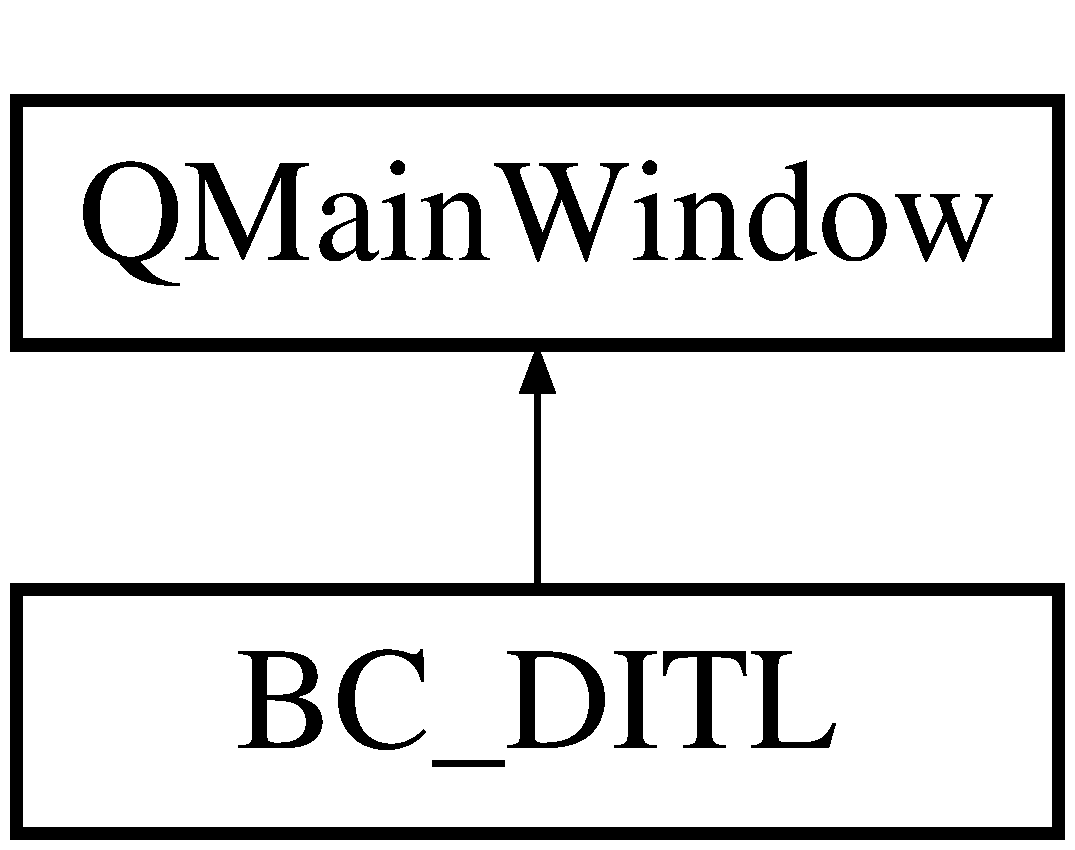
\includegraphics[height=2.000000cm]{class_b_c___d_i_t_l}
\end{center}
\end{figure}
\subsection*{Signals}
\begin{DoxyCompactItemize}
\item 
void {\bfseries dying} ()\hypertarget{class_b_c___d_i_t_l_a606f51e2d6c026e1198c3a2d0a5c17f0}{}\label{class_b_c___d_i_t_l_a606f51e2d6c026e1198c3a2d0a5c17f0}

\end{DoxyCompactItemize}
\subsection*{Public Member Functions}
\begin{DoxyCompactItemize}
\item 
{\bfseries B\+C\+\_\+\+D\+I\+TL} (Q\+Widget $\ast$parent=0)\hypertarget{class_b_c___d_i_t_l_a47efff48da269b402d29e458726023d9}{}\label{class_b_c___d_i_t_l_a47efff48da269b402d29e458726023d9}

\item 
\hyperlink{class_b_c___d_i_t_l_a9a570b8e6b5304a0f96748bc0eb69cd1}{$\sim$\+B\+C\+\_\+\+D\+I\+TL} ()\hypertarget{class_b_c___d_i_t_l_a9a570b8e6b5304a0f96748bc0eb69cd1}{}\label{class_b_c___d_i_t_l_a9a570b8e6b5304a0f96748bc0eb69cd1}

\begin{DoxyCompactList}\small\item\em Deletes the UI object. \end{DoxyCompactList}\end{DoxyCompactItemize}
\subsection*{Protected Member Functions}
\begin{DoxyCompactItemize}
\item 
void {\bfseries close\+Event} (Q\+Close\+Event $\ast$)\hypertarget{class_b_c___d_i_t_l_a102cbea9e530ddaf14989ab558799c6d}{}\label{class_b_c___d_i_t_l_a102cbea9e530ddaf14989ab558799c6d}

\end{DoxyCompactItemize}


The documentation for this class was generated from the following files\+:\begin{DoxyCompactItemize}
\item 
/home/riley/work/fsw/src/isatgs/\+B\+A\+R\+Co\+Mm\+S/src/modules/\+B\+A\+R\+Co\+Mm\+S\+\_\+\+D\+I\+T\+L/bc\+\_\+ditl.\+h\item 
/home/riley/work/fsw/src/isatgs/\+B\+A\+R\+Co\+Mm\+S/src/modules/\+B\+A\+R\+Co\+Mm\+S\+\_\+\+D\+I\+T\+L/bc\+\_\+ditl.\+cpp\item 
/home/riley/work/fsw/src/isatgs/\+B\+A\+R\+Co\+Mm\+S/src/modules/\+B\+A\+R\+Co\+Mm\+S\+\_\+\+D\+I\+T\+L/bc\+\_\+ditl\+\_\+add\+Event.\+cpp\item 
/home/riley/work/fsw/src/isatgs/\+B\+A\+R\+Co\+Mm\+S/src/modules/\+B\+A\+R\+Co\+Mm\+S\+\_\+\+D\+I\+T\+L/bc\+\_\+ditl\+\_\+init\+Event\+Name\+List.\+cpp\item 
/home/riley/work/fsw/src/isatgs/\+B\+A\+R\+Co\+Mm\+S/src/modules/\+B\+A\+R\+Co\+Mm\+S\+\_\+\+D\+I\+T\+L/bc\+\_\+ditl\+\_\+init\+Times.\+cpp\item 
/home/riley/work/fsw/src/isatgs/\+B\+A\+R\+Co\+Mm\+S/src/modules/\+B\+A\+R\+Co\+Mm\+S\+\_\+\+D\+I\+T\+L/bc\+\_\+ditl\+\_\+pdu\+Received.\+cpp\item 
/home/riley/work/fsw/src/isatgs/\+B\+A\+R\+Co\+Mm\+S/src/modules/\+B\+A\+R\+Co\+Mm\+S\+\_\+\+D\+I\+T\+L/bc\+\_\+ditl\+\_\+repaint.\+cpp\item 
/home/riley/work/fsw/src/isatgs/\+B\+A\+R\+Co\+Mm\+S/src/modules/\+B\+A\+R\+Co\+Mm\+S\+\_\+\+D\+I\+T\+L/bc\+\_\+ditl\+\_\+tree\+Item\+Clicked.\+cpp\item 
/home/riley/work/fsw/src/isatgs/\+B\+A\+R\+Co\+Mm\+S/src/modules/\+B\+A\+R\+Co\+Mm\+S\+\_\+\+D\+I\+T\+L/bc\+\_\+ditl\+\_\+utils.\+cpp\end{DoxyCompactItemize}

\hypertarget{class_b_c___d_i_t_l___e_v_e_n_t}{}\section{B\+C\+\_\+\+D\+I\+T\+L\+\_\+\+E\+V\+E\+NT Class Reference}
\label{class_b_c___d_i_t_l___e_v_e_n_t}\index{B\+C\+\_\+\+D\+I\+T\+L\+\_\+\+E\+V\+E\+NT@{B\+C\+\_\+\+D\+I\+T\+L\+\_\+\+E\+V\+E\+NT}}


The documentation for this class was generated from the following files\+:\begin{DoxyCompactItemize}
\item 
/home/riley/work/fsw/src/isatgs/\+B\+A\+R\+Co\+Mm\+S/src/modules/\+B\+A\+R\+Co\+Mm\+S\+\_\+\+D\+I\+T\+L/bc\+\_\+ditl\+\_\+event.\+h\item 
/home/riley/work/fsw/src/isatgs/\+B\+A\+R\+Co\+Mm\+S/src/modules/\+B\+A\+R\+Co\+Mm\+S\+\_\+\+D\+I\+T\+L/bc\+\_\+ditl\+\_\+event.\+cpp\end{DoxyCompactItemize}

\hypertarget{class_b_c___d_i_t_l___s_e_v_t_r_e_e___i_t_e_m}{}\section{B\+C\+\_\+\+D\+I\+T\+L\+\_\+\+S\+E\+V\+T\+R\+E\+E\+\_\+\+I\+T\+EM Class Reference}
\label{class_b_c___d_i_t_l___s_e_v_t_r_e_e___i_t_e_m}\index{B\+C\+\_\+\+D\+I\+T\+L\+\_\+\+S\+E\+V\+T\+R\+E\+E\+\_\+\+I\+T\+EM@{B\+C\+\_\+\+D\+I\+T\+L\+\_\+\+S\+E\+V\+T\+R\+E\+E\+\_\+\+I\+T\+EM}}
\subsection*{Public Member Functions}
\begin{DoxyCompactItemize}
\item 
{\bfseries B\+C\+\_\+\+D\+I\+T\+L\+\_\+\+S\+E\+V\+T\+R\+E\+E\+\_\+\+I\+T\+EM} (B\+C\+\_\+\+Event\+::\+Severity, std\+::string, std\+::string, double, double, double, double, bool)\hypertarget{class_b_c___d_i_t_l___s_e_v_t_r_e_e___i_t_e_m_a04966b5ef09bc4ac678e389c8d459d3a}{}\label{class_b_c___d_i_t_l___s_e_v_t_r_e_e___i_t_e_m_a04966b5ef09bc4ac678e389c8d459d3a}

\item 
void {\bfseries clean} ()\hypertarget{class_b_c___d_i_t_l___s_e_v_t_r_e_e___i_t_e_m_af9e3ddafe2a929b9d7bdd636affa403b}{}\label{class_b_c___d_i_t_l___s_e_v_t_r_e_e___i_t_e_m_af9e3ddafe2a929b9d7bdd636affa403b}

\end{DoxyCompactItemize}
\subsection*{Public Attributes}
\begin{DoxyCompactItemize}
\item 
B\+C\+\_\+\+Event\+::\+Severity {\bfseries sev}\hypertarget{class_b_c___d_i_t_l___s_e_v_t_r_e_e___i_t_e_m_ad0bb1ac98d29f041cfdce6d587605cab}{}\label{class_b_c___d_i_t_l___s_e_v_t_r_e_e___i_t_e_m_ad0bb1ac98d29f041cfdce6d587605cab}

\item 
Q\+Tree\+Widget\+Item $\ast$ {\bfseries child}\hypertarget{class_b_c___d_i_t_l___s_e_v_t_r_e_e___i_t_e_m_a5bd26cf9e8a12b443c9e5e0f78658884}{}\label{class_b_c___d_i_t_l___s_e_v_t_r_e_e___i_t_e_m_a5bd26cf9e8a12b443c9e5e0f78658884}

\item 
Q\+Tree\+Widget\+Item $\ast$ {\bfseries item}\hypertarget{class_b_c___d_i_t_l___s_e_v_t_r_e_e___i_t_e_m_a9279a959b2f52e7f81c7e538a79f1a89}{}\label{class_b_c___d_i_t_l___s_e_v_t_r_e_e___i_t_e_m_a9279a959b2f52e7f81c7e538a79f1a89}

\item 
std\+::string {\bfseries details}\hypertarget{class_b_c___d_i_t_l___s_e_v_t_r_e_e___i_t_e_m_a489e80599055c8029e42337e1a90bb66}{}\label{class_b_c___d_i_t_l___s_e_v_t_r_e_e___i_t_e_m_a489e80599055c8029e42337e1a90bb66}

\item 
std\+::string {\bfseries name}\hypertarget{class_b_c___d_i_t_l___s_e_v_t_r_e_e___i_t_e_m_afad2d3520f0ae750e994c81f5f6c1714}{}\label{class_b_c___d_i_t_l___s_e_v_t_r_e_e___i_t_e_m_afad2d3520f0ae750e994c81f5f6c1714}

\item 
double {\bfseries x}\hypertarget{class_b_c___d_i_t_l___s_e_v_t_r_e_e___i_t_e_m_a798d76b7682876858fb279bd29a8dabd}{}\label{class_b_c___d_i_t_l___s_e_v_t_r_e_e___i_t_e_m_a798d76b7682876858fb279bd29a8dabd}

\item 
double {\bfseries y}\hypertarget{class_b_c___d_i_t_l___s_e_v_t_r_e_e___i_t_e_m_a90f81b1edbcf767f3ae66d925205932a}{}\label{class_b_c___d_i_t_l___s_e_v_t_r_e_e___i_t_e_m_a90f81b1edbcf767f3ae66d925205932a}

\item 
double {\bfseries w}\hypertarget{class_b_c___d_i_t_l___s_e_v_t_r_e_e___i_t_e_m_acba7f441a7a738d977ec4d9504468095}{}\label{class_b_c___d_i_t_l___s_e_v_t_r_e_e___i_t_e_m_acba7f441a7a738d977ec4d9504468095}

\item 
double {\bfseries h}\hypertarget{class_b_c___d_i_t_l___s_e_v_t_r_e_e___i_t_e_m_ae97065747aa890fc19ac7696d1a45fc0}{}\label{class_b_c___d_i_t_l___s_e_v_t_r_e_e___i_t_e_m_ae97065747aa890fc19ac7696d1a45fc0}

\item 
bool {\bfseries is\+Point}\hypertarget{class_b_c___d_i_t_l___s_e_v_t_r_e_e___i_t_e_m_a015703aa9c6a50a3b10cc317fba76f61}{}\label{class_b_c___d_i_t_l___s_e_v_t_r_e_e___i_t_e_m_a015703aa9c6a50a3b10cc317fba76f61}

\end{DoxyCompactItemize}


The documentation for this class was generated from the following files\+:\begin{DoxyCompactItemize}
\item 
/home/riley/work/fsw/src/isatgs/\+B\+A\+R\+Co\+Mm\+S/src/modules/\+B\+A\+R\+Co\+Mm\+S\+\_\+\+D\+I\+T\+L/bc\+\_\+ditl\+\_\+sev\+Tree\+Item.\+h\item 
/home/riley/work/fsw/src/isatgs/\+B\+A\+R\+Co\+Mm\+S/src/modules/\+B\+A\+R\+Co\+Mm\+S\+\_\+\+D\+I\+T\+L/bc\+\_\+ditl\+\_\+sev\+Tree\+Item.\+cpp\end{DoxyCompactItemize}

\hypertarget{class_b_c___event}{}\section{B\+C\+\_\+\+Event Class Reference}
\label{class_b_c___event}\index{B\+C\+\_\+\+Event@{B\+C\+\_\+\+Event}}
\subsection*{Public Types}
\begin{DoxyCompactItemize}
\item 
enum {\bfseries Severity} \{ {\bfseries A\+D\+V\+I\+S\+O\+RY} = 0, 
{\bfseries C\+A\+U\+T\+I\+ON} = 1, 
{\bfseries W\+A\+R\+N\+I\+NG} = 2
 \}\hypertarget{class_b_c___event_a5eb4855476ea60e493118e250e27ea1e}{}\label{class_b_c___event_a5eb4855476ea60e493118e250e27ea1e}

\item 
enum {\bfseries Event\+Type} \{ {\bfseries P\+O\+I\+NT} = 0, 
{\bfseries S\+T\+A\+RT} = 1, 
{\bfseries E\+ND} = 2
 \}\hypertarget{class_b_c___event_af0659c0fa8f9fad210dc9be784232b19}{}\label{class_b_c___event_af0659c0fa8f9fad210dc9be784232b19}

\end{DoxyCompactItemize}
\subsection*{Public Member Functions}
\begin{DoxyCompactItemize}
\item 
{\bfseries B\+C\+\_\+\+Event} (uint64\+\_\+t, int, int, int, int, std\+::string, std\+::string, int)\hypertarget{class_b_c___event_a68ce3b239302b717104c8eb7f40e4bef}{}\label{class_b_c___event_a68ce3b239302b717104c8eb7f40e4bef}

\item 
{\bfseries B\+C\+\_\+\+Event} (std\+::string in)\hypertarget{class_b_c___event_af78e84637a9875dec516e185f35c1d1c}{}\label{class_b_c___event_af78e84637a9875dec516e185f35c1d1c}

\item 
Q\+Date\+Time {\bfseries get\+U\+TC} ()\hypertarget{class_b_c___event_a1760bf16d64ca7f717c8802b4a59df4d}{}\label{class_b_c___event_a1760bf16d64ca7f717c8802b4a59df4d}

\item 
bool {\bfseries read} (std\+::string in)\hypertarget{class_b_c___event_aae93e7ef80d9e7884391835dfe95cdcf}{}\label{class_b_c___event_aae93e7ef80d9e7884391835dfe95cdcf}

\item 
bool {\bfseries write} (std\+::fstream \&out)\hypertarget{class_b_c___event_af5ed2ed542f460db793ad623b9aacd3a}{}\label{class_b_c___event_af5ed2ed542f460db793ad623b9aacd3a}

\end{DoxyCompactItemize}
\subsection*{Static Public Member Functions}
\begin{DoxyCompactItemize}
\item 
static Q\+Date\+Time {\bfseries get\+U\+TC} (uint64\+\_\+t)\hypertarget{class_b_c___event_a3fc59df9986ed204e38c5ecb5cbf3a11}{}\label{class_b_c___event_a3fc59df9986ed204e38c5ecb5cbf3a11}

\end{DoxyCompactItemize}
\subsection*{Public Attributes}
\begin{DoxyCompactItemize}
\item 
uint64\+\_\+t {\bfseries time}\hypertarget{class_b_c___event_acd269f4dbdbdb27d4994998b6c669559}{}\label{class_b_c___event_acd269f4dbdbdb27d4994998b6c669559}

\item 
int {\bfseries code}\hypertarget{class_b_c___event_ac6686c20f280941419bf8c6fc9d7cb44}{}\label{class_b_c___event_ac6686c20f280941419bf8c6fc9d7cb44}

\item 
int {\bfseries origin}\hypertarget{class_b_c___event_a4a67d0557454551f825a01fa77872db7}{}\label{class_b_c___event_a4a67d0557454551f825a01fa77872db7}

\item 
Event\+Type {\bfseries event\+Type}\hypertarget{class_b_c___event_a7fb69f25ec2f6fa377d680d140c61d99}{}\label{class_b_c___event_a7fb69f25ec2f6fa377d680d140c61d99}

\item 
Severity {\bfseries severity}\hypertarget{class_b_c___event_a8ea390d80d78ac9800b929611fcbff20}{}\label{class_b_c___event_a8ea390d80d78ac9800b929611fcbff20}

\item 
std\+::string {\bfseries message}\hypertarget{class_b_c___event_aff93fcb88a819232bd85f4328939b9a9}{}\label{class_b_c___event_aff93fcb88a819232bd85f4328939b9a9}

\item 
std\+::string {\bfseries filename}\hypertarget{class_b_c___event_aae5aeacf68d313f8c0473510a5eb9388}{}\label{class_b_c___event_aae5aeacf68d313f8c0473510a5eb9388}

\item 
int {\bfseries line\+Number}\hypertarget{class_b_c___event_ace00f024ebc3e5e00f9472768c84a563}{}\label{class_b_c___event_ace00f024ebc3e5e00f9472768c84a563}

\end{DoxyCompactItemize}


The documentation for this class was generated from the following files\+:\begin{DoxyCompactItemize}
\item 
/home/riley/work/fsw/src/isatgs/\+B\+A\+R\+Co\+Mm\+S/src/dependencies/bc\+\_\+\+Event.\+h\item 
/home/riley/work/fsw/src/isatgs/\+B\+A\+R\+Co\+Mm\+S/src/dependencies/bc\+\_\+\+Event.\+cpp\end{DoxyCompactItemize}

\hypertarget{class_b_c___f_s_w_command}{}\section{B\+C\+\_\+\+F\+S\+W\+Command Class Reference}
\label{class_b_c___f_s_w_command}\index{B\+C\+\_\+\+F\+S\+W\+Command@{B\+C\+\_\+\+F\+S\+W\+Command}}
Inheritance diagram for B\+C\+\_\+\+F\+S\+W\+Command\+:\begin{figure}[H]
\begin{center}
\leavevmode
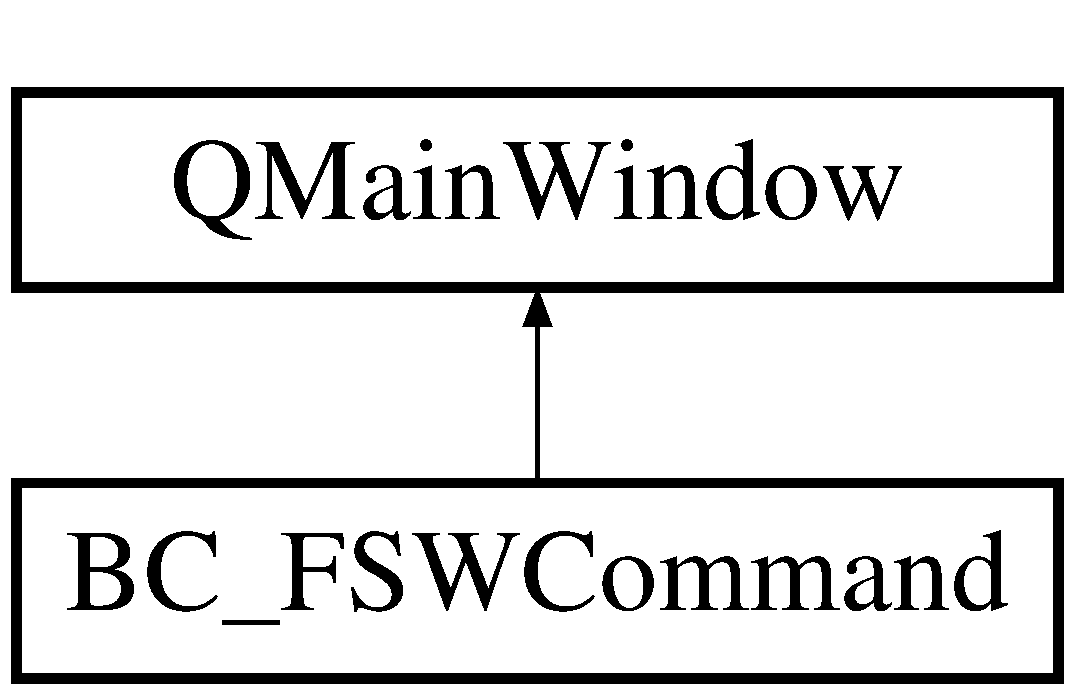
\includegraphics[height=2.000000cm]{class_b_c___f_s_w_command}
\end{center}
\end{figure}
\subsection*{Public Slots}
\begin{DoxyCompactItemize}
\item 
void {\bfseries fsw\+\_\+command} ()\hypertarget{class_b_c___f_s_w_command_ac62d04e1a233b8be6c0282a6b190e871}{}\label{class_b_c___f_s_w_command_ac62d04e1a233b8be6c0282a6b190e871}

\item 
void {\bfseries downlink\+\_\+buffer} ()\hypertarget{class_b_c___f_s_w_command_a829d42c42be3f705e5ae879458970464}{}\label{class_b_c___f_s_w_command_a829d42c42be3f705e5ae879458970464}

\item 
void {\bfseries ping} ()\hypertarget{class_b_c___f_s_w_command_a768755452dd9d3ea6f254faca4023475}{}\label{class_b_c___f_s_w_command_a768755452dd9d3ea6f254faca4023475}

\item 
void {\bfseries comm\+\_\+schedule} ()\hypertarget{class_b_c___f_s_w_command_ac89ad1d3184957b540b97fc6e66b0577}{}\label{class_b_c___f_s_w_command_ac89ad1d3184957b540b97fc6e66b0577}

\item 
void {\bfseries telem\+\_\+query} ()\hypertarget{class_b_c___f_s_w_command_a0cb08174939a6615c7b74f041f45c6c8}{}\label{class_b_c___f_s_w_command_a0cb08174939a6615c7b74f041f45c6c8}

\item 
void {\bfseries gnc} ()\hypertarget{class_b_c___f_s_w_command_ab45398a5264c3adde847f6ceaac16756}{}\label{class_b_c___f_s_w_command_ab45398a5264c3adde847f6ceaac16756}

\item 
void {\bfseries decom\+\_\+commit} ()\hypertarget{class_b_c___f_s_w_command_af0991d296ec2f2c783e947259705a266}{}\label{class_b_c___f_s_w_command_af0991d296ec2f2c783e947259705a266}

\item 
void {\bfseries decom\+\_\+enable} ()\hypertarget{class_b_c___f_s_w_command_a8c41449ae1b498e815993ff49ba929b3}{}\label{class_b_c___f_s_w_command_a8c41449ae1b498e815993ff49ba929b3}

\item 
void {\bfseries prop\+\_\+schedule} ()\hypertarget{class_b_c___f_s_w_command_ae496eb4dbfcaf3c638f1e43f1e5bd656}{}\label{class_b_c___f_s_w_command_ae496eb4dbfcaf3c638f1e43f1e5bd656}

\item 
void {\bfseries safe\+\_\+mode} ()\hypertarget{class_b_c___f_s_w_command_ae96a86eebb10245286e858fc169f3f4c}{}\label{class_b_c___f_s_w_command_ae96a86eebb10245286e858fc169f3f4c}

\item 
void {\bfseries oper\+\_\+mode} ()\hypertarget{class_b_c___f_s_w_command_a8ff7521a64184185e43739470870b477}{}\label{class_b_c___f_s_w_command_a8ff7521a64184185e43739470870b477}

\item 
void {\bfseries abort\+\_\+comm\+\_\+pass} ()\hypertarget{class_b_c___f_s_w_command_a97cd05d55b88c39c18164fe052926dcb}{}\label{class_b_c___f_s_w_command_a97cd05d55b88c39c18164fe052926dcb}

\item 
void {\bfseries set\+\_\+dev\+\_\+avail} ()\hypertarget{class_b_c___f_s_w_command_a8971142e43eb107158637769765d9af8}{}\label{class_b_c___f_s_w_command_a8971142e43eb107158637769765d9af8}

\item 
void {\bfseries set\+\_\+dev\+\_\+power} ()\hypertarget{class_b_c___f_s_w_command_a9d429d55692fd954d1616b1b8590943c}{}\label{class_b_c___f_s_w_command_a9d429d55692fd954d1616b1b8590943c}

\item 
void {\bfseries reset\+\_\+dev} ()\hypertarget{class_b_c___f_s_w_command_a0da93361d89985d07d6a5f046a656db1}{}\label{class_b_c___f_s_w_command_a0da93361d89985d07d6a5f046a656db1}

\item 
void {\bfseries fsw\+\_\+restart} ()\hypertarget{class_b_c___f_s_w_command_a1b60c256115d8a282a4120fdfc6fbf84}{}\label{class_b_c___f_s_w_command_a1b60c256115d8a282a4120fdfc6fbf84}

\item 
void {\bfseries fsw\+\_\+reboot} ()\hypertarget{class_b_c___f_s_w_command_aa9ab8f696f172bcd41ffffd9c0707b7e}{}\label{class_b_c___f_s_w_command_aa9ab8f696f172bcd41ffffd9c0707b7e}

\item 
void {\bfseries transmit\+\_\+data\+\_\+rate} ()\hypertarget{class_b_c___f_s_w_command_a1928dc27cfd06a7940449e3581b9cb49}{}\label{class_b_c___f_s_w_command_a1928dc27cfd06a7940449e3581b9cb49}

\item 
void {\bfseries event\+\_\+retrans} ()\hypertarget{class_b_c___f_s_w_command_ab6bb3e28f6d4cf06a0731e54821fbeaf}{}\label{class_b_c___f_s_w_command_ab6bb3e28f6d4cf06a0731e54821fbeaf}

\item 
void {\bfseries camera\+\_\+capture\+\_\+img} ()\hypertarget{class_b_c___f_s_w_command_a3b9e432ab284d82a39a508823dfcb29a}{}\label{class_b_c___f_s_w_command_a3b9e432ab284d82a39a508823dfcb29a}

\item 
void {\bfseries send\+\_\+camera\+\_\+capture\+\_\+img} (int, int)\hypertarget{class_b_c___f_s_w_command_a19969904ede1151e8ffcf33d066553e5}{}\label{class_b_c___f_s_w_command_a19969904ede1151e8ffcf33d066553e5}

\item 
void {\bfseries camera\+\_\+download\+\_\+imgs} ()\hypertarget{class_b_c___f_s_w_command_ad9007bc89d10d29f646f7d9976d550e3}{}\label{class_b_c___f_s_w_command_ad9007bc89d10d29f646f7d9976d550e3}

\item 
void {\bfseries send\+\_\+camera\+\_\+download\+\_\+imgs} (int)\hypertarget{class_b_c___f_s_w_command_a58c56b43b794844e29ceeaa90d381518}{}\label{class_b_c___f_s_w_command_a58c56b43b794844e29ceeaa90d381518}

\item 
void {\bfseries take\+Other} (Byte\+Buffer)\hypertarget{class_b_c___f_s_w_command_a144ebee256b1585e75c2a3088f5b9ac7}{}\label{class_b_c___f_s_w_command_a144ebee256b1585e75c2a3088f5b9ac7}

\item 
void {\bfseries display\+R\+S\+SI} (int)\hypertarget{class_b_c___f_s_w_command_aa9392d3146b9868f447a3dbf91d6b51a}{}\label{class_b_c___f_s_w_command_aa9392d3146b9868f447a3dbf91d6b51a}

\item 
void {\bfseries pdu\+Received} ()\hypertarget{class_b_c___f_s_w_command_a0ed16123648f649eb58122dad5e6b86e}{}\label{class_b_c___f_s_w_command_a0ed16123648f649eb58122dad5e6b86e}

\item 
void {\bfseries tel\+Act\+Off} ()\hypertarget{class_b_c___f_s_w_command_a7d9560a21829e36ee7d5f3ab3d46a3fe}{}\label{class_b_c___f_s_w_command_a7d9560a21829e36ee7d5f3ab3d46a3fe}

\end{DoxyCompactItemize}
\subsection*{Signals}
\begin{DoxyCompactItemize}
\item 
void {\bfseries command\+Sent} (int apid, int id)\hypertarget{class_b_c___f_s_w_command_a497a0fc1b67d4f6ec294ac96de8e7392}{}\label{class_b_c___f_s_w_command_a497a0fc1b67d4f6ec294ac96de8e7392}

\item 
void {\bfseries dying} ()\hypertarget{class_b_c___f_s_w_command_a80b774b6b647f1ed333ca836717487a1}{}\label{class_b_c___f_s_w_command_a80b774b6b647f1ed333ca836717487a1}

\end{DoxyCompactItemize}
\subsection*{Public Member Functions}
\begin{DoxyCompactItemize}
\item 
{\bfseries B\+C\+\_\+\+F\+S\+W\+Command} (Q\+Widget $\ast$parent=0)\hypertarget{class_b_c___f_s_w_command_a43ac12045e383c6b5a688bc6de1cfb5d}{}\label{class_b_c___f_s_w_command_a43ac12045e383c6b5a688bc6de1cfb5d}

\item 
void {\bfseries close\+Event} (Q\+Close\+Event $\ast$)\hypertarget{class_b_c___f_s_w_command_a45bf341a14d5bb88f96dcdd8080ceece}{}\label{class_b_c___f_s_w_command_a45bf341a14d5bb88f96dcdd8080ceece}

\end{DoxyCompactItemize}
\subsection*{Public Attributes}
\begin{DoxyCompactItemize}
\item 
\hyperlink{class_u_d_p_connection}{U\+D\+P\+Connection} {\bfseries connection}\hypertarget{class_b_c___f_s_w_command_a547d93f42f8950ecd93f52a12ac85155}{}\label{class_b_c___f_s_w_command_a547d93f42f8950ecd93f52a12ac85155}

\item 
End\+Point {\bfseries src}\hypertarget{class_b_c___f_s_w_command_a6ee66e652e72da22e71b1ef9b08740e3}{}\label{class_b_c___f_s_w_command_a6ee66e652e72da22e71b1ef9b08740e3}

\item 
End\+Point {\bfseries dest}\hypertarget{class_b_c___f_s_w_command_ac88bd114f14bbc078f5381f555675e8d}{}\label{class_b_c___f_s_w_command_ac88bd114f14bbc078f5381f555675e8d}

\item 
Byte\+Buffer {\bfseries buf}\hypertarget{class_b_c___f_s_w_command_a23dcb64b80b18693b5e06af12a852342}{}\label{class_b_c___f_s_w_command_a23dcb64b80b18693b5e06af12a852342}

\item 
Q\+Message\+Box $\ast$ {\bfseries msg\+Exit}\hypertarget{class_b_c___f_s_w_command_a74f5a0cbb7dd8c6b66112c5788b3bcac}{}\label{class_b_c___f_s_w_command_a74f5a0cbb7dd8c6b66112c5788b3bcac}

\item 
int {\bfseries number\+Of\+Commands}\hypertarget{class_b_c___f_s_w_command_a474add68e8053415c0bf84a3472c8775}{}\label{class_b_c___f_s_w_command_a474add68e8053415c0bf84a3472c8775}

\item 
Q\+File {\bfseries cmd\+Seq\+Id\+File}\hypertarget{class_b_c___f_s_w_command_ad0ee749d7f6a947d3c0d3fc870854484}{}\label{class_b_c___f_s_w_command_ad0ee749d7f6a947d3c0d3fc870854484}

\item 
\hyperlink{class_camera___capture___img___window}{Camera\+\_\+\+Capture\+\_\+\+Img\+\_\+\+Window} $\ast$ {\bfseries camera\+Capture\+Img\+Window}\hypertarget{class_b_c___f_s_w_command_ae179a0832323d2730d2f9caeb3492f64}{}\label{class_b_c___f_s_w_command_ae179a0832323d2730d2f9caeb3492f64}

\item 
\hyperlink{class_camera___download___imgs___window}{Camera\+\_\+\+Download\+\_\+\+Imgs\+\_\+\+Window} $\ast$ {\bfseries camera\+Download\+Imgs\+Window}\hypertarget{class_b_c___f_s_w_command_adb251f1c2609a8cf78d5b41dfff1023f}{}\label{class_b_c___f_s_w_command_adb251f1c2609a8cf78d5b41dfff1023f}

\item 
Q\+L\+C\+D\+Number $\ast$ {\bfseries R\+S\+SI}\hypertarget{class_b_c___f_s_w_command_a47653239d9de4d5e3a4873a819724210}{}\label{class_b_c___f_s_w_command_a47653239d9de4d5e3a4873a819724210}

\item 
Q\+Graphics\+Scene $\ast$ {\bfseries tel\+Act}\hypertarget{class_b_c___f_s_w_command_ac325d45d18052b6dabc15ac04844cea0}{}\label{class_b_c___f_s_w_command_ac325d45d18052b6dabc15ac04844cea0}

\item 
Q\+Graphics\+Ellipse\+Item $\ast$ {\bfseries tel\+Act\+Light}\hypertarget{class_b_c___f_s_w_command_a9770d402fb9105744836fbfd2bfa458a}{}\label{class_b_c___f_s_w_command_a9770d402fb9105744836fbfd2bfa458a}

\item 
Q\+Timer $\ast$ {\bfseries tel\+Act\+Timer} = new Q\+Timer()\hypertarget{class_b_c___f_s_w_command_ad4ae190549649ef2d1bb8e2e216c3408}{}\label{class_b_c___f_s_w_command_ad4ae190549649ef2d1bb8e2e216c3408}

\end{DoxyCompactItemize}


The documentation for this class was generated from the following files\+:\begin{DoxyCompactItemize}
\item 
/home/riley/work/fsw/src/isatgs/\+B\+A\+R\+Co\+Mm\+S/src/modules/\+B\+A\+R\+Co\+Mm\+S\+\_\+\+Command/bc\+\_\+fswcommand.\+h\item 
/home/riley/work/fsw/src/isatgs/\+B\+A\+R\+Co\+Mm\+S/src/modules/\+B\+A\+R\+Co\+Mm\+S\+\_\+\+Command/bc\+\_\+fswcommand.\+cpp\end{DoxyCompactItemize}

\hypertarget{class_b_c___packet_listener_thread}{}\section{B\+C\+\_\+\+Packet\+Listener\+Thread Class Reference}
\label{class_b_c___packet_listener_thread}\index{B\+C\+\_\+\+Packet\+Listener\+Thread@{B\+C\+\_\+\+Packet\+Listener\+Thread}}
Inheritance diagram for B\+C\+\_\+\+Packet\+Listener\+Thread\+:\begin{figure}[H]
\begin{center}
\leavevmode
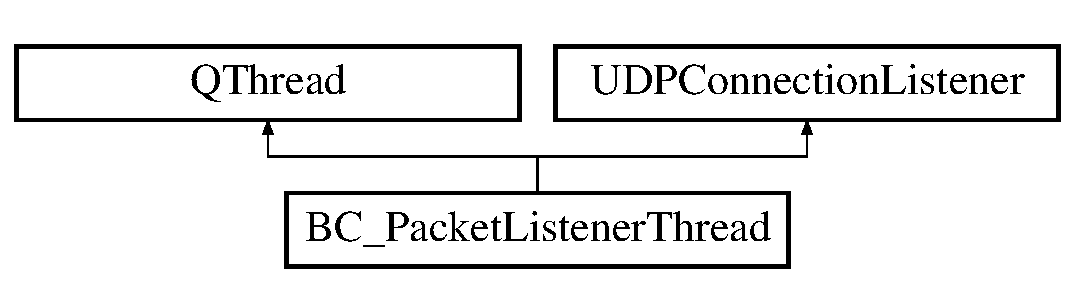
\includegraphics[height=2.000000cm]{class_b_c___packet_listener_thread}
\end{center}
\end{figure}
\subsection*{Public Slots}
\begin{DoxyCompactItemize}
\item 
void {\bfseries user\+Died} ()\hypertarget{class_b_c___packet_listener_thread_a8e64484e475cb1b1f125ab670abbfcaa}{}\label{class_b_c___packet_listener_thread_a8e64484e475cb1b1f125ab670abbfcaa}

\end{DoxyCompactItemize}
\subsection*{Signals}
\begin{DoxyCompactItemize}
\item 
void {\bfseries pdu\+Emit} (\hyperlink{classisat__utils_1_1_byte_buffer}{Byte\+Buffer})\hypertarget{class_b_c___packet_listener_thread_a397607b1bd8c9ae5fcaae3b8c7e92a0c}{}\label{class_b_c___packet_listener_thread_a397607b1bd8c9ae5fcaae3b8c7e92a0c}

\end{DoxyCompactItemize}
\subsection*{Public Member Functions}
\begin{DoxyCompactItemize}
\item 
{\bfseries B\+C\+\_\+\+Packet\+Listener\+Thread} (uint\+\_\+fast8\+\_\+t, int)\hypertarget{class_b_c___packet_listener_thread_ab2b75706eb9cb7cf1765edb8a989690b}{}\label{class_b_c___packet_listener_thread_ab2b75706eb9cb7cf1765edb8a989690b}

\item 
void {\bfseries run} ()\hypertarget{class_b_c___packet_listener_thread_a07449138555f5a789192989f565f143c}{}\label{class_b_c___packet_listener_thread_a07449138555f5a789192989f565f143c}

\item 
void {\bfseries pdu\+Received} (\hyperlink{class_u_d_p_connection}{U\+D\+P\+Connection} \&, \hyperlink{class_p_d_u}{P\+DU})\hypertarget{class_b_c___packet_listener_thread_a86562b977acc43b809c1e2af3dfbf14a}{}\label{class_b_c___packet_listener_thread_a86562b977acc43b809c1e2af3dfbf14a}

\end{DoxyCompactItemize}


The documentation for this class was generated from the following files\+:\begin{DoxyCompactItemize}
\item 
/home/riley/work/fsw/src/isatgs/\+B\+A\+R\+Co\+Mm\+S/src/dependencies/bc\+\_\+\+Packet\+Listener\+Thread.\+h\item 
/home/riley/work/fsw/src/isatgs/\+B\+A\+R\+Co\+Mm\+S/src/dependencies/bc\+\_\+\+Packet\+Listener\+Thread.\+cpp\end{DoxyCompactItemize}

\hypertarget{class_buffer}{}\section{Buffer Class Reference}
\label{class_buffer}\index{Buffer@{Buffer}}
Inheritance diagram for Buffer\+:\begin{figure}[H]
\begin{center}
\leavevmode
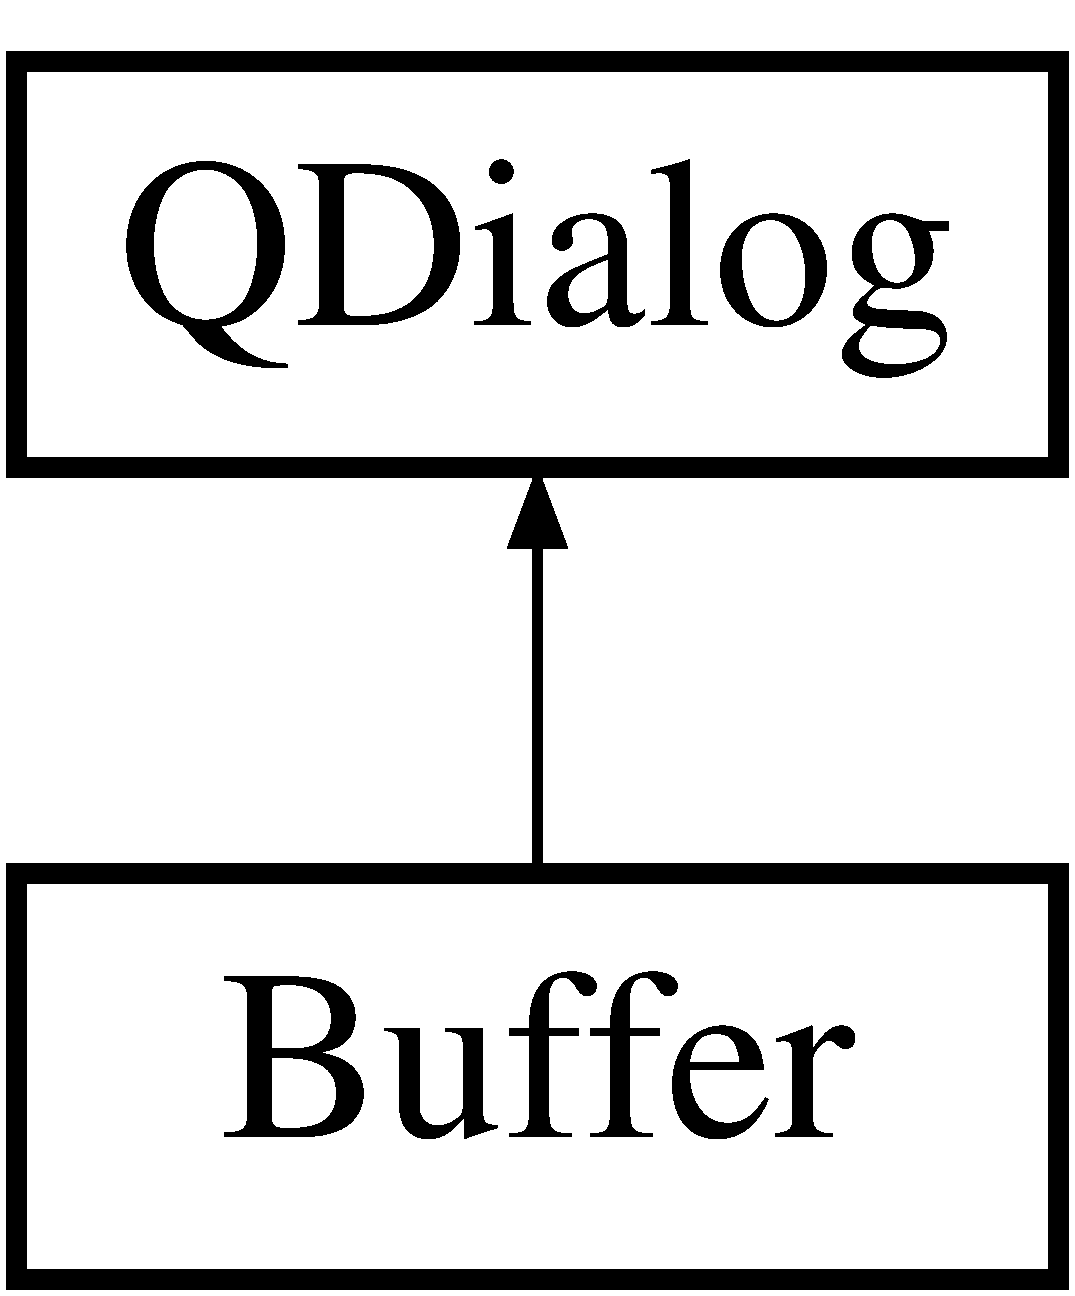
\includegraphics[height=2.000000cm]{class_buffer}
\end{center}
\end{figure}
\subsection*{Signals}
\begin{DoxyCompactItemize}
\item 
void {\bfseries buffer\+\_\+modify\+Buffer} (unsigned int buffer\+Size)\hypertarget{class_buffer_ac717991545d4c5351af9a713b91b2782}{}\label{class_buffer_ac717991545d4c5351af9a713b91b2782}

\end{DoxyCompactItemize}
\subsection*{Public Member Functions}
\begin{DoxyCompactItemize}
\item 
{\bfseries Buffer} (Q\+Widget $\ast$parent=0)\hypertarget{class_buffer_a70e8ab4821634d4d44b76d12e08a4dfe}{}\label{class_buffer_a70e8ab4821634d4d44b76d12e08a4dfe}

\item 
void {\bfseries buffer\+\_\+change\+Load\+Vals} ()\hypertarget{class_buffer_a52c5a7a3121aa5f9fc5cc39b1f5a801e}{}\label{class_buffer_a52c5a7a3121aa5f9fc5cc39b1f5a801e}

\end{DoxyCompactItemize}
\subsection*{Public Attributes}
\begin{DoxyCompactItemize}
\item 
unsigned int {\bfseries buffer\+Size}\hypertarget{class_buffer_a811467a3681514d9f7d1fed6fa0189d7}{}\label{class_buffer_a811467a3681514d9f7d1fed6fa0189d7}

\end{DoxyCompactItemize}


The documentation for this class was generated from the following files\+:\begin{DoxyCompactItemize}
\item 
/home/riley/work/fsw/src/isatgs/\+B\+A\+R\+Co\+Mm\+S/src/modules/\+B\+A\+R\+Co\+Mm\+S\+\_\+\+C\+F\+D\+P/buffer.\+h\item 
/home/riley/work/fsw/src/isatgs/\+B\+A\+R\+Co\+Mm\+S/src/modules/\+B\+A\+R\+Co\+Mm\+S\+\_\+\+C\+F\+D\+P/buffer.\+cpp\end{DoxyCompactItemize}

\hypertarget{classisat__utils_1_1_byte_buffer}{}\section{isat\+\_\+utils\+:\+:Byte\+Buffer Class Reference}
\label{classisat__utils_1_1_byte_buffer}\index{isat\+\_\+utils\+::\+Byte\+Buffer@{isat\+\_\+utils\+::\+Byte\+Buffer}}


{\ttfamily \#include $<$Byte\+Buffer.\+h$>$}

\subsection*{Public Types}
\begin{DoxyCompactItemize}
\item 
enum {\bfseries Byte\+Order} \{ {\bfseries Little\+Endian}, 
{\bfseries Big\+Endian}
 \}\hypertarget{classisat__utils_1_1_byte_buffer_a23d178f62dad62bad876f2350d3a552d}{}\label{classisat__utils_1_1_byte_buffer_a23d178f62dad62bad876f2350d3a552d}

\end{DoxyCompactItemize}
\subsection*{Public Member Functions}
\begin{DoxyCompactItemize}
\item 
\hyperlink{classisat__utils_1_1_byte_buffer_a9f4312493a433a005346b3f777d82c2a}{Byte\+Buffer} (int max\+Size=100)
\item 
{\bfseries Byte\+Buffer} (\hyperlink{classisat__utils_1_1_byte_buffer}{Byte\+Buffer} const \&rhs)\hypertarget{classisat__utils_1_1_byte_buffer_aac59d94f64a6e230092bb58a231f17ad}{}\label{classisat__utils_1_1_byte_buffer_aac59d94f64a6e230092bb58a231f17ad}

\item 
\hyperlink{classisat__utils_1_1_byte_buffer}{Byte\+Buffer} \& {\bfseries operator=} (\hyperlink{classisat__utils_1_1_byte_buffer}{Byte\+Buffer} rhs)\hypertarget{classisat__utils_1_1_byte_buffer_ae9e5d0ce671455c3ea0ef6b1177b6545}{}\label{classisat__utils_1_1_byte_buffer_ae9e5d0ce671455c3ea0ef6b1177b6545}

\item 
void \hyperlink{classisat__utils_1_1_byte_buffer_aba7629c0a1f32a7c8bc1fb0b7aa25d84}{clear} ()
\item 
bool \hyperlink{classisat__utils_1_1_byte_buffer_a713fea8a50894c0de09c5bac0a75d5f6}{seek} (int pos)
\item 
int \hyperlink{classisat__utils_1_1_byte_buffer_ac7936db245374ce1a91f50974108bf81}{get\+Position} () const 
\item 
int {\bfseries get\+Limit} () const \hypertarget{classisat__utils_1_1_byte_buffer_a916ff3ebb1c1f3b5961ed4518a57778a}{}\label{classisat__utils_1_1_byte_buffer_a916ff3ebb1c1f3b5961ed4518a57778a}

\item 
int {\bfseries get\+Capacity} () const \hypertarget{classisat__utils_1_1_byte_buffer_ae82ac9a8ea9a9cbad5017dbb9f3264f6}{}\label{classisat__utils_1_1_byte_buffer_ae82ac9a8ea9a9cbad5017dbb9f3264f6}

\item 
char const $\ast$ \hyperlink{classisat__utils_1_1_byte_buffer_abfd9c2f3bce4061d1e6111d6196bf652}{get\+Bytes} () const 
\item 
void {\bfseries set\+Byte\+Order} (Byte\+Order order)\hypertarget{classisat__utils_1_1_byte_buffer_a441e4ae0439dcef442075d9e9e702d5b}{}\label{classisat__utils_1_1_byte_buffer_a441e4ae0439dcef442075d9e9e702d5b}

\item 
Byte\+Order {\bfseries get\+Byte\+Order} ()\hypertarget{classisat__utils_1_1_byte_buffer_a06221da5fbdcac9152d88cb016e66aa5}{}\label{classisat__utils_1_1_byte_buffer_a06221da5fbdcac9152d88cb016e66aa5}

\item 
Byte\+Order {\bfseries get\+Native\+Byte\+Order} ()\hypertarget{classisat__utils_1_1_byte_buffer_ab383182e5a092503093a89335abdddb2}{}\label{classisat__utils_1_1_byte_buffer_ab383182e5a092503093a89335abdddb2}

\item 
bool \hyperlink{classisat__utils_1_1_byte_buffer_a6fff89c596eb04a8d243cdffd1f66251}{zero} (int count)
\item 
bool \hyperlink{classisat__utils_1_1_byte_buffer_a5848cebe8b234adb5c7f0af5b681c4b0}{put} (char const $\ast$data, int length)
\item 
bool {\bfseries put\+Byte} (unsigned char val)\hypertarget{classisat__utils_1_1_byte_buffer_ae30167db8302a7e5bea6e9136e7f7ea2}{}\label{classisat__utils_1_1_byte_buffer_ae30167db8302a7e5bea6e9136e7f7ea2}

\item 
bool {\bfseries put\+Boolean} (bool val)\hypertarget{classisat__utils_1_1_byte_buffer_aa29da52c50958b667699aa46a68a5601}{}\label{classisat__utils_1_1_byte_buffer_aa29da52c50958b667699aa46a68a5601}

\item 
bool {\bfseries put\+Short} (short val)\hypertarget{classisat__utils_1_1_byte_buffer_add15695017738c951656b9b4f9a9030f}{}\label{classisat__utils_1_1_byte_buffer_add15695017738c951656b9b4f9a9030f}

\item 
bool {\bfseries put\+Int} (int val)\hypertarget{classisat__utils_1_1_byte_buffer_a7cb40c1f7b3de249c0513dfbd9fd14c4}{}\label{classisat__utils_1_1_byte_buffer_a7cb40c1f7b3de249c0513dfbd9fd14c4}

\item 
bool {\bfseries put\+Float} (float val)\hypertarget{classisat__utils_1_1_byte_buffer_adc2c6670c58549309e7ae6ec84f80ab1}{}\label{classisat__utils_1_1_byte_buffer_adc2c6670c58549309e7ae6ec84f80ab1}

\item 
bool {\bfseries put\+Double} (double val)\hypertarget{classisat__utils_1_1_byte_buffer_ae6fceb8b47c53a046500966fb42ddac3}{}\label{classisat__utils_1_1_byte_buffer_ae6fceb8b47c53a046500966fb42ddac3}

\item 
bool {\bfseries put\+Int32} (int32\+\_\+t val)\hypertarget{classisat__utils_1_1_byte_buffer_ab0571342a4da94a0096bbda428f98e91}{}\label{classisat__utils_1_1_byte_buffer_ab0571342a4da94a0096bbda428f98e91}

\item 
bool {\bfseries put\+Int64} (int64\+\_\+t val)\hypertarget{classisat__utils_1_1_byte_buffer_a17a34eecf26a3cf8357fcf3d168d32df}{}\label{classisat__utils_1_1_byte_buffer_a17a34eecf26a3cf8357fcf3d168d32df}

\item 
bool {\bfseries put\+Uint32} (uint32\+\_\+t val)\hypertarget{classisat__utils_1_1_byte_buffer_ab4a52f2f98b8d82a0f49dfa2092f66f4}{}\label{classisat__utils_1_1_byte_buffer_ab4a52f2f98b8d82a0f49dfa2092f66f4}

\item 
bool {\bfseries put\+Uint64} (uint64\+\_\+t val)\hypertarget{classisat__utils_1_1_byte_buffer_a50a7fe8e470bba38c30043c7762c35f2}{}\label{classisat__utils_1_1_byte_buffer_a50a7fe8e470bba38c30043c7762c35f2}

\item 
bool {\bfseries get\+Byte} (unsigned char \&val)\hypertarget{classisat__utils_1_1_byte_buffer_a9e0713e2d91b9500ab07bc79f6b8dab7}{}\label{classisat__utils_1_1_byte_buffer_a9e0713e2d91b9500ab07bc79f6b8dab7}

\item 
bool {\bfseries get\+Boolean} (bool \&value)\hypertarget{classisat__utils_1_1_byte_buffer_a920085ab7a5ec2ac058817b0562e61ca}{}\label{classisat__utils_1_1_byte_buffer_a920085ab7a5ec2ac058817b0562e61ca}

\item 
bool {\bfseries get\+Short} (short \&value)\hypertarget{classisat__utils_1_1_byte_buffer_ab053198353e8472f4abb10cbc89ea1a7}{}\label{classisat__utils_1_1_byte_buffer_ab053198353e8472f4abb10cbc89ea1a7}

\item 
bool {\bfseries get\+Int} (int \&value)\hypertarget{classisat__utils_1_1_byte_buffer_a05344c817b39e5ffd6061ef034e79782}{}\label{classisat__utils_1_1_byte_buffer_a05344c817b39e5ffd6061ef034e79782}

\item 
bool {\bfseries get\+Float} (float \&value)\hypertarget{classisat__utils_1_1_byte_buffer_a8d18929321a12811b0adf4dd6a7bde97}{}\label{classisat__utils_1_1_byte_buffer_a8d18929321a12811b0adf4dd6a7bde97}

\item 
bool {\bfseries get\+Double} (double \&value)\hypertarget{classisat__utils_1_1_byte_buffer_a38b08e1eb87881f0a17e4a839d79a2ba}{}\label{classisat__utils_1_1_byte_buffer_a38b08e1eb87881f0a17e4a839d79a2ba}

\item 
bool {\bfseries get\+Int32} (int32\+\_\+t \&value)\hypertarget{classisat__utils_1_1_byte_buffer_a4b5f0b6bc42393ce0854afccae1e8ba2}{}\label{classisat__utils_1_1_byte_buffer_a4b5f0b6bc42393ce0854afccae1e8ba2}

\item 
bool {\bfseries get\+Int64} (int64\+\_\+t \&value)\hypertarget{classisat__utils_1_1_byte_buffer_a8dbe370b9cd2f40486712a918d5974c9}{}\label{classisat__utils_1_1_byte_buffer_a8dbe370b9cd2f40486712a918d5974c9}

\item 
bool {\bfseries get\+Uint32} (uint32\+\_\+t \&value)\hypertarget{classisat__utils_1_1_byte_buffer_a8505094c9a0ab612c24b9386821630cf}{}\label{classisat__utils_1_1_byte_buffer_a8505094c9a0ab612c24b9386821630cf}

\item 
bool {\bfseries get\+Uint64} (uint64\+\_\+t \&value)\hypertarget{classisat__utils_1_1_byte_buffer_a80a6474146c84f119c4d25e2de8f69c6}{}\label{classisat__utils_1_1_byte_buffer_a80a6474146c84f119c4d25e2de8f69c6}

\item 
bool {\bfseries get\+Bits} (int bit\+Offset, int bit\+Width, int \&value)\hypertarget{classisat__utils_1_1_byte_buffer_a1e3ff2ed80f8ab63a9a318b17176014c}{}\label{classisat__utils_1_1_byte_buffer_a1e3ff2ed80f8ab63a9a318b17176014c}

\item 
bool {\bfseries put\+Bits} (int bit\+Offset, int bit\+Width, int value)\hypertarget{classisat__utils_1_1_byte_buffer_adf5fc993d9f2d0c8f3df067e62197d7d}{}\label{classisat__utils_1_1_byte_buffer_adf5fc993d9f2d0c8f3df067e62197d7d}

\end{DoxyCompactItemize}
\subsection*{Protected Member Functions}
\begin{DoxyCompactItemize}
\item 
void {\bfseries swap\+Instance} (\hyperlink{classisat__utils_1_1_byte_buffer}{Byte\+Buffer} \&rhs)\hypertarget{classisat__utils_1_1_byte_buffer_aca1b50580a58c9aabc912b8eb6543987}{}\label{classisat__utils_1_1_byte_buffer_aca1b50580a58c9aabc912b8eb6543987}

\end{DoxyCompactItemize}
\subsection*{Protected Attributes}
\begin{DoxyCompactItemize}
\item 
char $\ast$ {\bfseries buffer}\hypertarget{classisat__utils_1_1_byte_buffer_ac5c56d68ba13c03a2440d6ba4738cff3}{}\label{classisat__utils_1_1_byte_buffer_ac5c56d68ba13c03a2440d6ba4738cff3}

\item 
int {\bfseries max\+Size}\hypertarget{classisat__utils_1_1_byte_buffer_a165cc673c8169eaabd88b0c2ce3df2a3}{}\label{classisat__utils_1_1_byte_buffer_a165cc673c8169eaabd88b0c2ce3df2a3}

\item 
int {\bfseries pos}\hypertarget{classisat__utils_1_1_byte_buffer_a42ba2c311d4b680899933035a26421ae}{}\label{classisat__utils_1_1_byte_buffer_a42ba2c311d4b680899933035a26421ae}

\item 
int {\bfseries limit}\hypertarget{classisat__utils_1_1_byte_buffer_a718e92cd1132e3e0562698398bbf016a}{}\label{classisat__utils_1_1_byte_buffer_a718e92cd1132e3e0562698398bbf016a}

\item 
Byte\+Order {\bfseries byte\+Order}\hypertarget{classisat__utils_1_1_byte_buffer_a66654b19b70e006eb7d64a589bc8a842}{}\label{classisat__utils_1_1_byte_buffer_a66654b19b70e006eb7d64a589bc8a842}

\item 
Byte\+Order {\bfseries native\+Byte\+Order}\hypertarget{classisat__utils_1_1_byte_buffer_ab8e39542ef1a07385c62ed6cdc58d4a9}{}\label{classisat__utils_1_1_byte_buffer_ab8e39542ef1a07385c62ed6cdc58d4a9}

\end{DoxyCompactItemize}


\subsection{Detailed Description}
A buffer of bytes with useful get/set methods.

Modelled after Java\textquotesingle{}s class of the same name. This class wraps a buffer of bytes and provides get and set methods for various types commonly found in network packets. The byte order can be switch back and forth, even between gets (some packet formats have both big and little endian byte orders. Annoying.)

The abstraction is a buffer with a maximum size and a current read/write pointer. Reading or writing advances the pointer by the size of whatever was read. 

\subsection{Constructor \& Destructor Documentation}
\index{isat\+\_\+utils\+::\+Byte\+Buffer@{isat\+\_\+utils\+::\+Byte\+Buffer}!Byte\+Buffer@{Byte\+Buffer}}
\index{Byte\+Buffer@{Byte\+Buffer}!isat\+\_\+utils\+::\+Byte\+Buffer@{isat\+\_\+utils\+::\+Byte\+Buffer}}
\subsubsection[{\texorpdfstring{Byte\+Buffer(int max\+Size=100)}{ByteBuffer(int maxSize=100)}}]{\setlength{\rightskip}{0pt plus 5cm}isat\+\_\+utils\+::\+Byte\+Buffer\+::\+Byte\+Buffer (
\begin{DoxyParamCaption}
\item[{int}]{max\+Size = {\ttfamily 100}}
\end{DoxyParamCaption}
)}\hypertarget{classisat__utils_1_1_byte_buffer_a9f4312493a433a005346b3f777d82c2a}{}\label{classisat__utils_1_1_byte_buffer_a9f4312493a433a005346b3f777d82c2a}
Create a \hyperlink{classisat__utils_1_1_byte_buffer}{Byte\+Buffer} capable of holding up to maxsize bytes. 

\subsection{Member Function Documentation}
\index{isat\+\_\+utils\+::\+Byte\+Buffer@{isat\+\_\+utils\+::\+Byte\+Buffer}!clear@{clear}}
\index{clear@{clear}!isat\+\_\+utils\+::\+Byte\+Buffer@{isat\+\_\+utils\+::\+Byte\+Buffer}}
\subsubsection[{\texorpdfstring{clear()}{clear()}}]{\setlength{\rightskip}{0pt plus 5cm}void isat\+\_\+utils\+::\+Byte\+Buffer\+::clear (
\begin{DoxyParamCaption}
{}
\end{DoxyParamCaption}
)}\hypertarget{classisat__utils_1_1_byte_buffer_aba7629c0a1f32a7c8bc1fb0b7aa25d84}{}\label{classisat__utils_1_1_byte_buffer_aba7629c0a1f32a7c8bc1fb0b7aa25d84}
Clears the buffer by resetting the read/write pointer to zero. identical to seek(0). \index{isat\+\_\+utils\+::\+Byte\+Buffer@{isat\+\_\+utils\+::\+Byte\+Buffer}!get\+Bytes@{get\+Bytes}}
\index{get\+Bytes@{get\+Bytes}!isat\+\_\+utils\+::\+Byte\+Buffer@{isat\+\_\+utils\+::\+Byte\+Buffer}}
\subsubsection[{\texorpdfstring{get\+Bytes() const }{getBytes() const }}]{\setlength{\rightskip}{0pt plus 5cm}char const $\ast$ isat\+\_\+utils\+::\+Byte\+Buffer\+::get\+Bytes (
\begin{DoxyParamCaption}
{}
\end{DoxyParamCaption}
) const}\hypertarget{classisat__utils_1_1_byte_buffer_abfd9c2f3bce4061d1e6111d6196bf652}{}\label{classisat__utils_1_1_byte_buffer_abfd9c2f3bce4061d1e6111d6196bf652}
Return a pointer to the raw bytes in this instance. \index{isat\+\_\+utils\+::\+Byte\+Buffer@{isat\+\_\+utils\+::\+Byte\+Buffer}!get\+Position@{get\+Position}}
\index{get\+Position@{get\+Position}!isat\+\_\+utils\+::\+Byte\+Buffer@{isat\+\_\+utils\+::\+Byte\+Buffer}}
\subsubsection[{\texorpdfstring{get\+Position() const }{getPosition() const }}]{\setlength{\rightskip}{0pt plus 5cm}int isat\+\_\+utils\+::\+Byte\+Buffer\+::get\+Position (
\begin{DoxyParamCaption}
{}
\end{DoxyParamCaption}
) const}\hypertarget{classisat__utils_1_1_byte_buffer_ac7936db245374ce1a91f50974108bf81}{}\label{classisat__utils_1_1_byte_buffer_ac7936db245374ce1a91f50974108bf81}
\begin{DoxyReturn}{Returns}
The current offset of the read/write pointer. 
\end{DoxyReturn}
\index{isat\+\_\+utils\+::\+Byte\+Buffer@{isat\+\_\+utils\+::\+Byte\+Buffer}!put@{put}}
\index{put@{put}!isat\+\_\+utils\+::\+Byte\+Buffer@{isat\+\_\+utils\+::\+Byte\+Buffer}}
\subsubsection[{\texorpdfstring{put(char const $\ast$data, int length)}{put(char const *data, int length)}}]{\setlength{\rightskip}{0pt plus 5cm}bool isat\+\_\+utils\+::\+Byte\+Buffer\+::put (
\begin{DoxyParamCaption}
\item[{char const $\ast$}]{data, }
\item[{int}]{length}
\end{DoxyParamCaption}
)}\hypertarget{classisat__utils_1_1_byte_buffer_a5848cebe8b234adb5c7f0af5b681c4b0}{}\label{classisat__utils_1_1_byte_buffer_a5848cebe8b234adb5c7f0af5b681c4b0}
Write length bytes from data into this instance\textquotesingle{}s buffer. \index{isat\+\_\+utils\+::\+Byte\+Buffer@{isat\+\_\+utils\+::\+Byte\+Buffer}!seek@{seek}}
\index{seek@{seek}!isat\+\_\+utils\+::\+Byte\+Buffer@{isat\+\_\+utils\+::\+Byte\+Buffer}}
\subsubsection[{\texorpdfstring{seek(int pos)}{seek(int pos)}}]{\setlength{\rightskip}{0pt plus 5cm}bool isat\+\_\+utils\+::\+Byte\+Buffer\+::seek (
\begin{DoxyParamCaption}
\item[{int}]{pos}
\end{DoxyParamCaption}
)}\hypertarget{classisat__utils_1_1_byte_buffer_a713fea8a50894c0de09c5bac0a75d5f6}{}\label{classisat__utils_1_1_byte_buffer_a713fea8a50894c0de09c5bac0a75d5f6}
Move the read/write pointer to pos. \index{isat\+\_\+utils\+::\+Byte\+Buffer@{isat\+\_\+utils\+::\+Byte\+Buffer}!zero@{zero}}
\index{zero@{zero}!isat\+\_\+utils\+::\+Byte\+Buffer@{isat\+\_\+utils\+::\+Byte\+Buffer}}
\subsubsection[{\texorpdfstring{zero(int count)}{zero(int count)}}]{\setlength{\rightskip}{0pt plus 5cm}bool isat\+\_\+utils\+::\+Byte\+Buffer\+::zero (
\begin{DoxyParamCaption}
\item[{int}]{count}
\end{DoxyParamCaption}
)}\hypertarget{classisat__utils_1_1_byte_buffer_a6fff89c596eb04a8d243cdffd1f66251}{}\label{classisat__utils_1_1_byte_buffer_a6fff89c596eb04a8d243cdffd1f66251}
Write count zero bytes into buffer at current location. 

The documentation for this class was generated from the following files\+:\begin{DoxyCompactItemize}
\item 
/home/riley/work/fsw/src/isatgs/\+B\+A\+R\+Co\+Mm\+S/src/dependencies/utils/Byte\+Buffer.\+h\item 
/home/riley/work/fsw/src/isatgs/\+B\+A\+R\+Co\+Mm\+S/src/dependencies/utils/Byte\+Buffer.\+cpp\end{DoxyCompactItemize}

\hypertarget{class_camera___capture___img___window}{}\section{Camera\+\_\+\+Capture\+\_\+\+Img\+\_\+\+Window Class Reference}
\label{class_camera___capture___img___window}\index{Camera\+\_\+\+Capture\+\_\+\+Img\+\_\+\+Window@{Camera\+\_\+\+Capture\+\_\+\+Img\+\_\+\+Window}}
Inheritance diagram for Camera\+\_\+\+Capture\+\_\+\+Img\+\_\+\+Window\+:\begin{figure}[H]
\begin{center}
\leavevmode
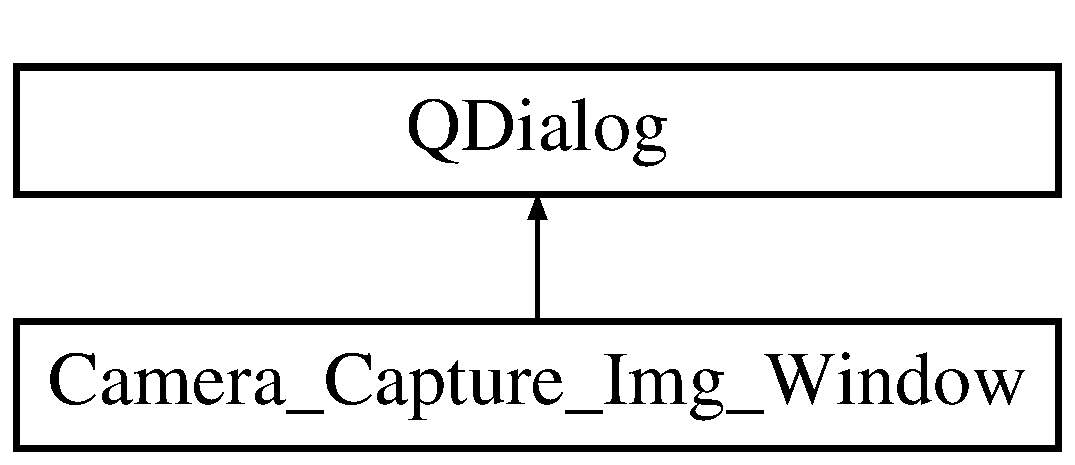
\includegraphics[height=2.000000cm]{class_camera___capture___img___window}
\end{center}
\end{figure}
\subsection*{Signals}
\begin{DoxyCompactItemize}
\item 
void {\bfseries fields} (int, int)\hypertarget{class_camera___capture___img___window_acfd4dea631a3cf2948fec802ceb4f595}{}\label{class_camera___capture___img___window_acfd4dea631a3cf2948fec802ceb4f595}

\end{DoxyCompactItemize}
\subsection*{Public Member Functions}
\begin{DoxyCompactItemize}
\item 
{\bfseries Camera\+\_\+\+Capture\+\_\+\+Img\+\_\+\+Window} (Q\+Widget $\ast$parent=0)\hypertarget{class_camera___capture___img___window_a63bb99e4f3782b80279a7926a9a9cd1b}{}\label{class_camera___capture___img___window_a63bb99e4f3782b80279a7926a9a9cd1b}

\item 
void {\bfseries close\+Event} (Q\+Close\+Event $\ast$)\hypertarget{class_camera___capture___img___window_aa737ef4694501d231be76b701e887a9c}{}\label{class_camera___capture___img___window_aa737ef4694501d231be76b701e887a9c}

\end{DoxyCompactItemize}
\subsection*{Public Attributes}
\begin{DoxyCompactItemize}
\item 
Q\+Slider $\ast$ {\bfseries avg\+Brightness\+Edit} = new Q\+Slider()\hypertarget{class_camera___capture___img___window_a5b687b585b4d29b277d8f69b521a9c51}{}\label{class_camera___capture___img___window_a5b687b585b4d29b277d8f69b521a9c51}

\item 
Q\+Slider $\ast$ {\bfseries fill\+Edit} = new Q\+Slider()\hypertarget{class_camera___capture___img___window_a452c7674f459af25a7648b8905a1f8c2}{}\label{class_camera___capture___img___window_a452c7674f459af25a7648b8905a1f8c2}

\item 
int {\bfseries avg\+Brightness}\hypertarget{class_camera___capture___img___window_a0e106b401683866ab721d170bc8db4fa}{}\label{class_camera___capture___img___window_a0e106b401683866ab721d170bc8db4fa}

\item 
int {\bfseries fill}\hypertarget{class_camera___capture___img___window_ab19dbab3c1b5e12e1b5242b50203a42a}{}\label{class_camera___capture___img___window_ab19dbab3c1b5e12e1b5242b50203a42a}

\end{DoxyCompactItemize}


The documentation for this class was generated from the following files\+:\begin{DoxyCompactItemize}
\item 
/home/riley/work/fsw/src/isatgs/\+B\+A\+R\+Co\+Mm\+S/src/modules/\+B\+A\+R\+Co\+Mm\+S\+\_\+\+Command/camera\+\_\+capture\+\_\+img\+\_\+window.\+h\item 
/home/riley/work/fsw/src/isatgs/\+B\+A\+R\+Co\+Mm\+S/src/modules/\+B\+A\+R\+Co\+Mm\+S\+\_\+\+Command/camera\+\_\+capture\+\_\+img\+\_\+window.\+cpp\end{DoxyCompactItemize}

\hypertarget{class_camera___download___imgs___window}{}\section{Camera\+\_\+\+Download\+\_\+\+Imgs\+\_\+\+Window Class Reference}
\label{class_camera___download___imgs___window}\index{Camera\+\_\+\+Download\+\_\+\+Imgs\+\_\+\+Window@{Camera\+\_\+\+Download\+\_\+\+Imgs\+\_\+\+Window}}
Inheritance diagram for Camera\+\_\+\+Download\+\_\+\+Imgs\+\_\+\+Window\+:\begin{figure}[H]
\begin{center}
\leavevmode
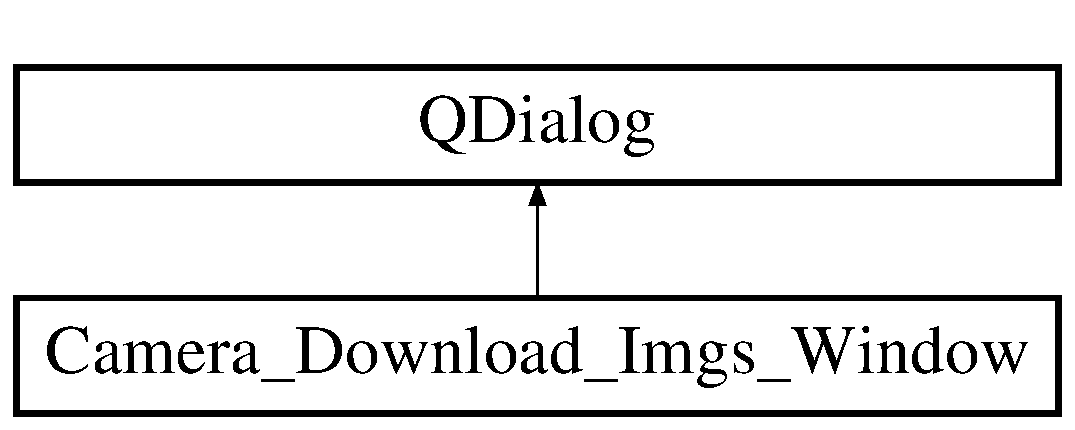
\includegraphics[height=2.000000cm]{class_camera___download___imgs___window}
\end{center}
\end{figure}
\subsection*{Signals}
\begin{DoxyCompactItemize}
\item 
void {\bfseries fields} (int)\hypertarget{class_camera___download___imgs___window_a388fe05d8eeb66483bf031907da11087}{}\label{class_camera___download___imgs___window_a388fe05d8eeb66483bf031907da11087}

\end{DoxyCompactItemize}
\subsection*{Public Member Functions}
\begin{DoxyCompactItemize}
\item 
{\bfseries Camera\+\_\+\+Download\+\_\+\+Imgs\+\_\+\+Window} (Q\+Widget $\ast$parent=0)\hypertarget{class_camera___download___imgs___window_aa305a3a0e8bf4362fdfae21fa4e0d01e}{}\label{class_camera___download___imgs___window_aa305a3a0e8bf4362fdfae21fa4e0d01e}

\item 
void {\bfseries close\+Event} (Q\+Close\+Event $\ast$)\hypertarget{class_camera___download___imgs___window_a449612cf2bd3304f0550bb319d898b8c}{}\label{class_camera___download___imgs___window_a449612cf2bd3304f0550bb319d898b8c}

\end{DoxyCompactItemize}
\subsection*{Public Attributes}
\begin{DoxyCompactItemize}
\item 
Q\+Spin\+Box $\ast$ {\bfseries num\+Images\+Edit}\hypertarget{class_camera___download___imgs___window_a62a219798180c816c20261128503b087}{}\label{class_camera___download___imgs___window_a62a219798180c816c20261128503b087}

\item 
int {\bfseries num\+Images}\hypertarget{class_camera___download___imgs___window_a26781cddb49073c988e23ec45ff1528e}{}\label{class_camera___download___imgs___window_a26781cddb49073c988e23ec45ff1528e}

\end{DoxyCompactItemize}


The documentation for this class was generated from the following files\+:\begin{DoxyCompactItemize}
\item 
/home/riley/work/fsw/src/isatgs/\+B\+A\+R\+Co\+Mm\+S/src/modules/\+B\+A\+R\+Co\+Mm\+S\+\_\+\+Command/camera\+\_\+download\+\_\+imgs\+\_\+window.\+h\item 
/home/riley/work/fsw/src/isatgs/\+B\+A\+R\+Co\+Mm\+S/src/modules/\+B\+A\+R\+Co\+Mm\+S\+\_\+\+Command/camera\+\_\+download\+\_\+imgs\+\_\+window.\+cpp\end{DoxyCompactItemize}

\hypertarget{classisat__trek_1_1_camera_capture_img___command}{}\section{isat\+\_\+trek\+:\+:Camera\+Capture\+Img\+\_\+\+Command Class Reference}
\label{classisat__trek_1_1_camera_capture_img___command}\index{isat\+\_\+trek\+::\+Camera\+Capture\+Img\+\_\+\+Command@{isat\+\_\+trek\+::\+Camera\+Capture\+Img\+\_\+\+Command}}


{\ttfamily \#include $<$Camera\+Capture\+Img\+\_\+\+Command.\+h$>$}

Inheritance diagram for isat\+\_\+trek\+:\+:Camera\+Capture\+Img\+\_\+\+Command\+:\begin{figure}[H]
\begin{center}
\leavevmode
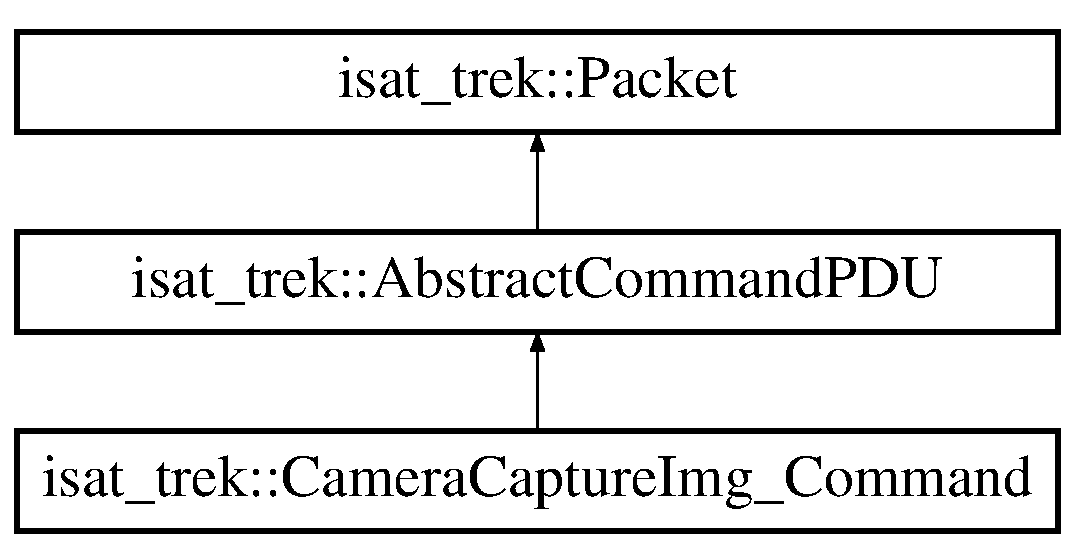
\includegraphics[height=3.000000cm]{classisat__trek_1_1_camera_capture_img___command}
\end{center}
\end{figure}
\subsection*{Public Member Functions}
\begin{DoxyCompactItemize}
\item 
bool \hyperlink{classisat__trek_1_1_camera_capture_img___command_ae766c5c98f697abf11370b8388f9c7d9}{from\+Bytes} (Byte\+Buffer \&buf)
\item 
bool \hyperlink{classisat__trek_1_1_camera_capture_img___command_ab7333d2572b3d73089b4e147f6104bcd}{to\+Bytes} (Byte\+Buffer \&buf)
\end{DoxyCompactItemize}
\subsection*{Public Attributes}
\begin{DoxyCompactItemize}
\item 
int {\bfseries avg\+Brightness}\hypertarget{classisat__trek_1_1_camera_capture_img___command_acc0042572a8c9772f080e5dd423869f3}{}\label{classisat__trek_1_1_camera_capture_img___command_acc0042572a8c9772f080e5dd423869f3}

\item 
int {\bfseries fill}\hypertarget{classisat__trek_1_1_camera_capture_img___command_a84bae9d631608a471a8b2a8c197ddf4d}{}\label{classisat__trek_1_1_camera_capture_img___command_a84bae9d631608a471a8b2a8c197ddf4d}

\end{DoxyCompactItemize}


\subsection{Detailed Description}
X\+XX\+: Replace with real description in isat.\+pdu file. 

\subsection{Member Function Documentation}
\index{isat\+\_\+trek\+::\+Camera\+Capture\+Img\+\_\+\+Command@{isat\+\_\+trek\+::\+Camera\+Capture\+Img\+\_\+\+Command}!from\+Bytes@{from\+Bytes}}
\index{from\+Bytes@{from\+Bytes}!isat\+\_\+trek\+::\+Camera\+Capture\+Img\+\_\+\+Command@{isat\+\_\+trek\+::\+Camera\+Capture\+Img\+\_\+\+Command}}
\subsubsection[{\texorpdfstring{from\+Bytes(\+Byte\+Buffer \&buf)}{fromBytes(ByteBuffer &buf)}}]{\setlength{\rightskip}{0pt plus 5cm}bool isat\+\_\+trek\+::\+Camera\+Capture\+Img\+\_\+\+Command\+::from\+Bytes (
\begin{DoxyParamCaption}
\item[{Byte\+Buffer \&}]{buf}
\end{DoxyParamCaption}
)\hspace{0.3cm}{\ttfamily [virtual]}}\hypertarget{classisat__trek_1_1_camera_capture_img___command_ae766c5c98f697abf11370b8388f9c7d9}{}\label{classisat__trek_1_1_camera_capture_img___command_ae766c5c98f697abf11370b8388f9c7d9}
Populate the header and command fields from the data in buf.

\begin{DoxyReturn}{Returns}
true if successful. 
\end{DoxyReturn}


Implements \hyperlink{classisat__trek_1_1_packet}{isat\+\_\+trek\+::\+Packet}.

\index{isat\+\_\+trek\+::\+Camera\+Capture\+Img\+\_\+\+Command@{isat\+\_\+trek\+::\+Camera\+Capture\+Img\+\_\+\+Command}!to\+Bytes@{to\+Bytes}}
\index{to\+Bytes@{to\+Bytes}!isat\+\_\+trek\+::\+Camera\+Capture\+Img\+\_\+\+Command@{isat\+\_\+trek\+::\+Camera\+Capture\+Img\+\_\+\+Command}}
\subsubsection[{\texorpdfstring{to\+Bytes(\+Byte\+Buffer \&buf)}{toBytes(ByteBuffer &buf)}}]{\setlength{\rightskip}{0pt plus 5cm}bool isat\+\_\+trek\+::\+Camera\+Capture\+Img\+\_\+\+Command\+::to\+Bytes (
\begin{DoxyParamCaption}
\item[{Byte\+Buffer \&}]{buf}
\end{DoxyParamCaption}
)\hspace{0.3cm}{\ttfamily [virtual]}}\hypertarget{classisat__trek_1_1_camera_capture_img___command_ab7333d2572b3d73089b4e147f6104bcd}{}\label{classisat__trek_1_1_camera_capture_img___command_ab7333d2572b3d73089b4e147f6104bcd}
Create the binary representation of this instance in the specified buffer.

\begin{DoxyReturn}{Returns}
true if successful. 
\end{DoxyReturn}


Implements \hyperlink{classisat__trek_1_1_packet}{isat\+\_\+trek\+::\+Packet}.



The documentation for this class was generated from the following files\+:\begin{DoxyCompactItemize}
\item 
/home/riley/work/fsw/src/isatgs/\+B\+A\+R\+Co\+Mm\+S/src/dependencies/trek/command/Camera\+Capture\+Img\+\_\+\+Command.\+h\item 
/home/riley/work/fsw/src/isatgs/\+B\+A\+R\+Co\+Mm\+S/src/dependencies/trek/command/Camera\+Capture\+Img\+\_\+\+Command.\+cpp\end{DoxyCompactItemize}

\hypertarget{classisat__trek_1_1_camera_download_imgs___command}{}\section{isat\+\_\+trek\+:\+:Camera\+Download\+Imgs\+\_\+\+Command Class Reference}
\label{classisat__trek_1_1_camera_download_imgs___command}\index{isat\+\_\+trek\+::\+Camera\+Download\+Imgs\+\_\+\+Command@{isat\+\_\+trek\+::\+Camera\+Download\+Imgs\+\_\+\+Command}}


{\ttfamily \#include $<$Camera\+Download\+Imgs\+\_\+\+Command.\+h$>$}

Inheritance diagram for isat\+\_\+trek\+:\+:Camera\+Download\+Imgs\+\_\+\+Command\+:\begin{figure}[H]
\begin{center}
\leavevmode
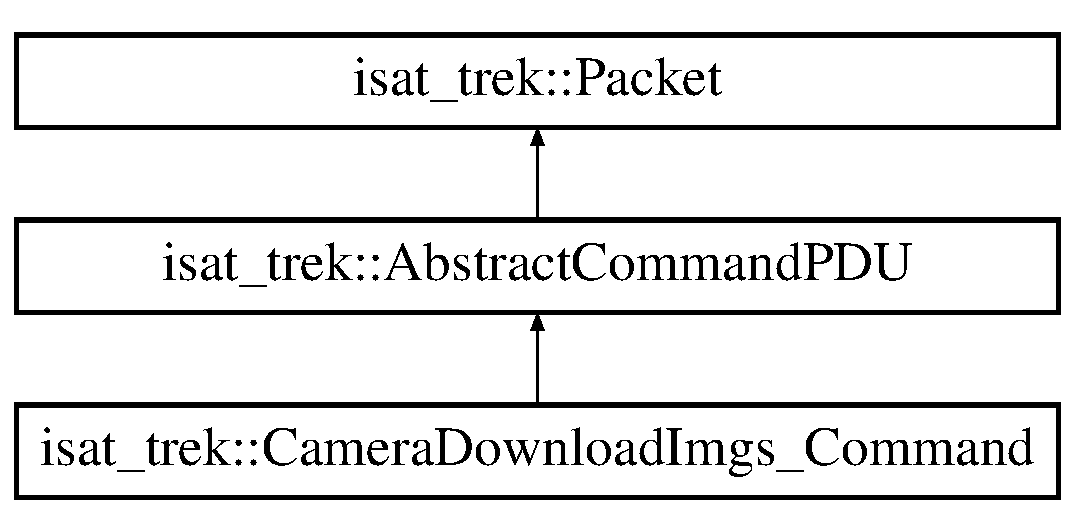
\includegraphics[height=3.000000cm]{classisat__trek_1_1_camera_download_imgs___command}
\end{center}
\end{figure}
\subsection*{Public Member Functions}
\begin{DoxyCompactItemize}
\item 
bool \hyperlink{classisat__trek_1_1_camera_download_imgs___command_a4578459c7137386128b7043cd1e7ecb9}{from\+Bytes} (Byte\+Buffer \&buf)
\item 
bool \hyperlink{classisat__trek_1_1_camera_download_imgs___command_a4273aeaf8bfef5ad5cb900c93b7b7e4a}{to\+Bytes} (Byte\+Buffer \&buf)
\end{DoxyCompactItemize}
\subsection*{Public Attributes}
\begin{DoxyCompactItemize}
\item 
int {\bfseries num\+Images}\hypertarget{classisat__trek_1_1_camera_download_imgs___command_a89b9fcceb637f01c2346d7f47e9a3dce}{}\label{classisat__trek_1_1_camera_download_imgs___command_a89b9fcceb637f01c2346d7f47e9a3dce}

\end{DoxyCompactItemize}


\subsection{Detailed Description}
X\+XX\+: Replace with real description in isat.\+pdu file. 

\subsection{Member Function Documentation}
\index{isat\+\_\+trek\+::\+Camera\+Download\+Imgs\+\_\+\+Command@{isat\+\_\+trek\+::\+Camera\+Download\+Imgs\+\_\+\+Command}!from\+Bytes@{from\+Bytes}}
\index{from\+Bytes@{from\+Bytes}!isat\+\_\+trek\+::\+Camera\+Download\+Imgs\+\_\+\+Command@{isat\+\_\+trek\+::\+Camera\+Download\+Imgs\+\_\+\+Command}}
\subsubsection[{\texorpdfstring{from\+Bytes(\+Byte\+Buffer \&buf)}{fromBytes(ByteBuffer &buf)}}]{\setlength{\rightskip}{0pt plus 5cm}bool isat\+\_\+trek\+::\+Camera\+Download\+Imgs\+\_\+\+Command\+::from\+Bytes (
\begin{DoxyParamCaption}
\item[{Byte\+Buffer \&}]{buf}
\end{DoxyParamCaption}
)\hspace{0.3cm}{\ttfamily [virtual]}}\hypertarget{classisat__trek_1_1_camera_download_imgs___command_a4578459c7137386128b7043cd1e7ecb9}{}\label{classisat__trek_1_1_camera_download_imgs___command_a4578459c7137386128b7043cd1e7ecb9}
Populate the header and command fields from the data in buf.

\begin{DoxyReturn}{Returns}
true if successful. 
\end{DoxyReturn}


Implements \hyperlink{classisat__trek_1_1_packet}{isat\+\_\+trek\+::\+Packet}.

\index{isat\+\_\+trek\+::\+Camera\+Download\+Imgs\+\_\+\+Command@{isat\+\_\+trek\+::\+Camera\+Download\+Imgs\+\_\+\+Command}!to\+Bytes@{to\+Bytes}}
\index{to\+Bytes@{to\+Bytes}!isat\+\_\+trek\+::\+Camera\+Download\+Imgs\+\_\+\+Command@{isat\+\_\+trek\+::\+Camera\+Download\+Imgs\+\_\+\+Command}}
\subsubsection[{\texorpdfstring{to\+Bytes(\+Byte\+Buffer \&buf)}{toBytes(ByteBuffer &buf)}}]{\setlength{\rightskip}{0pt plus 5cm}bool isat\+\_\+trek\+::\+Camera\+Download\+Imgs\+\_\+\+Command\+::to\+Bytes (
\begin{DoxyParamCaption}
\item[{Byte\+Buffer \&}]{buf}
\end{DoxyParamCaption}
)\hspace{0.3cm}{\ttfamily [virtual]}}\hypertarget{classisat__trek_1_1_camera_download_imgs___command_a4273aeaf8bfef5ad5cb900c93b7b7e4a}{}\label{classisat__trek_1_1_camera_download_imgs___command_a4273aeaf8bfef5ad5cb900c93b7b7e4a}
Create the binary representation of this instance in the specified buffer.

\begin{DoxyReturn}{Returns}
true if successful. 
\end{DoxyReturn}


Implements \hyperlink{classisat__trek_1_1_packet}{isat\+\_\+trek\+::\+Packet}.



The documentation for this class was generated from the following files\+:\begin{DoxyCompactItemize}
\item 
/home/riley/work/fsw/src/isatgs/\+B\+A\+R\+Co\+Mm\+S/src/dependencies/trek/command/Camera\+Download\+Imgs\+\_\+\+Command.\+h\item 
/home/riley/work/fsw/src/isatgs/\+B\+A\+R\+Co\+Mm\+S/src/dependencies/trek/command/Camera\+Download\+Imgs\+\_\+\+Command.\+cpp\end{DoxyCompactItemize}

\hypertarget{classisat__trek_1_1_c_c_s_d_s_telemetry_header}{}\section{isat\+\_\+trek\+:\+:C\+C\+S\+D\+S\+Telemetry\+Header Class Reference}
\label{classisat__trek_1_1_c_c_s_d_s_telemetry_header}\index{isat\+\_\+trek\+::\+C\+C\+S\+D\+S\+Telemetry\+Header@{isat\+\_\+trek\+::\+C\+C\+S\+D\+S\+Telemetry\+Header}}


{\ttfamily \#include $<$C\+C\+S\+D\+S\+Telemetry\+Header.\+h$>$}

\subsection*{Public Member Functions}
\begin{DoxyCompactItemize}
\item 
void {\bfseries to\+Bytes} (\hyperlink{classisat__utils_1_1_byte_buffer}{isat\+\_\+utils\+::\+Byte\+Buffer} \&buf)\hypertarget{classisat__trek_1_1_c_c_s_d_s_telemetry_header_a43d6355a1e75990cb6b57827b265cc4a}{}\label{classisat__trek_1_1_c_c_s_d_s_telemetry_header_a43d6355a1e75990cb6b57827b265cc4a}

\item 
void {\bfseries from\+Bytes} (\hyperlink{classisat__utils_1_1_byte_buffer}{isat\+\_\+utils\+::\+Byte\+Buffer} \&buf)\hypertarget{classisat__trek_1_1_c_c_s_d_s_telemetry_header_ad1b88c7c9321fa020ccf66d4057a25ed}{}\label{classisat__trek_1_1_c_c_s_d_s_telemetry_header_ad1b88c7c9321fa020ccf66d4057a25ed}

\end{DoxyCompactItemize}
\subsection*{Public Attributes}
\begin{DoxyCompactItemize}
\item 
int {\bfseries version}\hypertarget{classisat__trek_1_1_c_c_s_d_s_telemetry_header_a5cec65352d30539c10e6d9a1cc30a8cb}{}\label{classisat__trek_1_1_c_c_s_d_s_telemetry_header_a5cec65352d30539c10e6d9a1cc30a8cb}

\item 
int {\bfseries ptype}\hypertarget{classisat__trek_1_1_c_c_s_d_s_telemetry_header_ab73b461c8ae3639dc99adeaeb6159157}{}\label{classisat__trek_1_1_c_c_s_d_s_telemetry_header_ab73b461c8ae3639dc99adeaeb6159157}

\item 
int {\bfseries shf}\hypertarget{classisat__trek_1_1_c_c_s_d_s_telemetry_header_a293212a2ceefbc83092d01766f108223}{}\label{classisat__trek_1_1_c_c_s_d_s_telemetry_header_a293212a2ceefbc83092d01766f108223}

\item 
int {\bfseries apid}\hypertarget{classisat__trek_1_1_c_c_s_d_s_telemetry_header_a783153deaa42442ec761df88817b7f0b}{}\label{classisat__trek_1_1_c_c_s_d_s_telemetry_header_a783153deaa42442ec761df88817b7f0b}

\item 
int {\bfseries seq\+\_\+flags}\hypertarget{classisat__trek_1_1_c_c_s_d_s_telemetry_header_aedfff6c6431c9861c77c33090d0625ae}{}\label{classisat__trek_1_1_c_c_s_d_s_telemetry_header_aedfff6c6431c9861c77c33090d0625ae}

\item 
int {\bfseries seq\+\_\+count}\hypertarget{classisat__trek_1_1_c_c_s_d_s_telemetry_header_a7043f9eef87912483d88039369026659}{}\label{classisat__trek_1_1_c_c_s_d_s_telemetry_header_a7043f9eef87912483d88039369026659}

\item 
int {\bfseries pkt\+\_\+length}\hypertarget{classisat__trek_1_1_c_c_s_d_s_telemetry_header_aa8d6d92ebeb672a1e208c56338f5c71e}{}\label{classisat__trek_1_1_c_c_s_d_s_telemetry_header_aa8d6d92ebeb672a1e208c56338f5c71e}

\item 
int {\bfseries coarse\+\_\+time}\hypertarget{classisat__trek_1_1_c_c_s_d_s_telemetry_header_af089e3a17adc7d87f39aa7a753590c95}{}\label{classisat__trek_1_1_c_c_s_d_s_telemetry_header_af089e3a17adc7d87f39aa7a753590c95}

\item 
int {\bfseries fine\+\_\+time}\hypertarget{classisat__trek_1_1_c_c_s_d_s_telemetry_header_ab08fca8bacf5b8345a8dc927742de6a0}{}\label{classisat__trek_1_1_c_c_s_d_s_telemetry_header_ab08fca8bacf5b8345a8dc927742de6a0}

\item 
int {\bfseries sp\+\_\+source}\hypertarget{classisat__trek_1_1_c_c_s_d_s_telemetry_header_a8763710bdfb7e74a88025b12425e96f7}{}\label{classisat__trek_1_1_c_c_s_d_s_telemetry_header_a8763710bdfb7e74a88025b12425e96f7}

\item 
int {\bfseries trek\+\_\+seat}\hypertarget{classisat__trek_1_1_c_c_s_d_s_telemetry_header_a0993ceeaf9294fe285fa652cf962176e}{}\label{classisat__trek_1_1_c_c_s_d_s_telemetry_header_a0993ceeaf9294fe285fa652cf962176e}

\item 
int {\bfseries ancil\+\_\+data}\hypertarget{classisat__trek_1_1_c_c_s_d_s_telemetry_header_a3b9a8781ba758fd1795afbb2a97b24ad}{}\label{classisat__trek_1_1_c_c_s_d_s_telemetry_header_a3b9a8781ba758fd1795afbb2a97b24ad}

\end{DoxyCompactItemize}


\subsection{Detailed Description}
A \hyperlink{classisat__trek_1_1_c_c_s_d_s_telemetry_header}{C\+C\+S\+D\+S\+Telemetry\+Header} writes the required C\+C\+S\+DS Telemetry Header fields to the given Byte\+Buffer. (Really.. did you expect anything else with a name like \hyperlink{classisat__trek_1_1_c_c_s_d_s_telemetry_header}{C\+C\+S\+D\+S\+Telemetry\+Header}?) 

The documentation for this class was generated from the following files\+:\begin{DoxyCompactItemize}
\item 
/home/riley/work/fsw/src/isatgs/\+B\+A\+R\+Co\+Mm\+S/src/dependencies/trek/C\+C\+S\+D\+S\+Telemetry\+Header.\+h\item 
/home/riley/work/fsw/src/isatgs/\+B\+A\+R\+Co\+Mm\+S/src/dependencies/trek/C\+C\+S\+D\+S\+Telemetry\+Header.\+cpp\end{DoxyCompactItemize}

\hypertarget{struct_c_f_d_p___d_a_t_a}{}\section{C\+F\+D\+P\+\_\+\+D\+A\+TA Struct Reference}
\label{struct_c_f_d_p___d_a_t_a}\index{C\+F\+D\+P\+\_\+\+D\+A\+TA@{C\+F\+D\+P\+\_\+\+D\+A\+TA}}
\subsection*{Public Attributes}
\begin{DoxyCompactItemize}
\item 
u\+\_\+int\+\_\+4 {\bfseries length}\hypertarget{struct_c_f_d_p___d_a_t_a_aa821731a5a0d614582dd426dd40d5727}{}\label{struct_c_f_d_p___d_a_t_a_aa821731a5a0d614582dd426dd40d5727}

\item 
u\+\_\+int\+\_\+1 {\bfseries content} \mbox{[}M\+A\+X\+\_\+\+D\+A\+T\+A\+\_\+\+L\+E\+N\+G\+TH\mbox{]}\hypertarget{struct_c_f_d_p___d_a_t_a_aee1f28cda84b9c8858154a148f6cb137}{}\label{struct_c_f_d_p___d_a_t_a_aee1f28cda84b9c8858154a148f6cb137}

\end{DoxyCompactItemize}


The documentation for this struct was generated from the following file\+:\begin{DoxyCompactItemize}
\item 
/home/riley/work/fsw/src/isatgs/\+B\+A\+R\+Co\+Mm\+S/src/dependencies/\+C\+F\+D\+P/\+P\+U\+B/cfdp\+\_\+data\+\_\+structures.\+h\end{DoxyCompactItemize}

\hypertarget{struct_c_f_d_p___n_o_d_e}{}\section{C\+F\+D\+P\+\_\+\+N\+O\+DE Struct Reference}
\label{struct_c_f_d_p___n_o_d_e}\index{C\+F\+D\+P\+\_\+\+N\+O\+DE@{C\+F\+D\+P\+\_\+\+N\+O\+DE}}
\subsection*{Public Attributes}
\begin{DoxyCompactItemize}
\item 
F\+I\+LE $\ast$ {\bfseries fp\+\_\+from\+\_\+node}\hypertarget{struct_c_f_d_p___n_o_d_e_af6ffaa344a9b6e40469abc2c081fe65f}{}\label{struct_c_f_d_p___n_o_d_e_af6ffaa344a9b6e40469abc2c081fe65f}

\item 
F\+I\+LE $\ast$ {\bfseries fp\+\_\+to\+\_\+node}\hypertarget{struct_c_f_d_p___n_o_d_e_afdd351b40192588285680d245c9584a1}{}\label{struct_c_f_d_p___n_o_d_e_afdd351b40192588285680d245c9584a1}

\item 
char {\bfseries id} \mbox{[}M\+A\+X\+\_\+\+I\+D\+\_\+\+L\+E\+N\+G\+TH\mbox{]}\hypertarget{struct_c_f_d_p___n_o_d_e_a77b567349d5531d35eb56f9391b0b6e2}{}\label{struct_c_f_d_p___n_o_d_e_a77b567349d5531d35eb56f9391b0b6e2}

\end{DoxyCompactItemize}


The documentation for this struct was generated from the following file\+:\begin{DoxyCompactItemize}
\item 
/home/riley/work/fsw/src/isatgs/\+B\+A\+R\+Co\+Mm\+S/src/dependencies/\+C\+F\+D\+P/\+T\+E\+S\+T/test\+\_\+cfdp.\+c\end{DoxyCompactItemize}

\hypertarget{classisat__trek_1_1_change_mode___command}{}\section{isat\+\_\+trek\+:\+:Change\+Mode\+\_\+\+Command Class Reference}
\label{classisat__trek_1_1_change_mode___command}\index{isat\+\_\+trek\+::\+Change\+Mode\+\_\+\+Command@{isat\+\_\+trek\+::\+Change\+Mode\+\_\+\+Command}}


{\ttfamily \#include $<$Change\+Mode\+\_\+\+Command.\+h$>$}

Inheritance diagram for isat\+\_\+trek\+:\+:Change\+Mode\+\_\+\+Command\+:\begin{figure}[H]
\begin{center}
\leavevmode
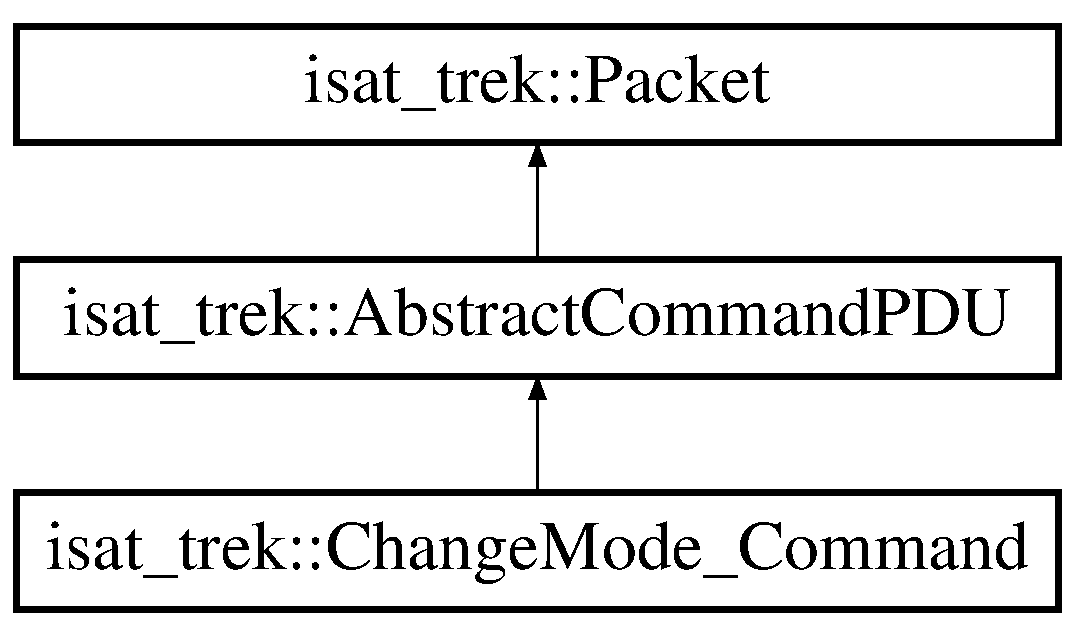
\includegraphics[height=3.000000cm]{classisat__trek_1_1_change_mode___command}
\end{center}
\end{figure}
\subsection*{Public Member Functions}
\begin{DoxyCompactItemize}
\item 
bool \hyperlink{classisat__trek_1_1_change_mode___command_a9b25f1596746890d0c4f93f089eadce6}{from\+Bytes} (Byte\+Buffer \&buf)
\item 
bool \hyperlink{classisat__trek_1_1_change_mode___command_abd1d9cdd783958408fad57595f28c110}{to\+Bytes} (Byte\+Buffer \&buf)
\end{DoxyCompactItemize}
\subsection*{Public Attributes}
\begin{DoxyCompactItemize}
\item 
int {\bfseries new\+Mode} = 0\hypertarget{classisat__trek_1_1_change_mode___command_a7755f2e017223ca39bd62ee72c83ca24}{}\label{classisat__trek_1_1_change_mode___command_a7755f2e017223ca39bd62ee72c83ca24}

\end{DoxyCompactItemize}


\subsection{Detailed Description}
X\+XX\+: Replace with real description in isat.\+pdu file. 

\subsection{Member Function Documentation}
\index{isat\+\_\+trek\+::\+Change\+Mode\+\_\+\+Command@{isat\+\_\+trek\+::\+Change\+Mode\+\_\+\+Command}!from\+Bytes@{from\+Bytes}}
\index{from\+Bytes@{from\+Bytes}!isat\+\_\+trek\+::\+Change\+Mode\+\_\+\+Command@{isat\+\_\+trek\+::\+Change\+Mode\+\_\+\+Command}}
\subsubsection[{\texorpdfstring{from\+Bytes(\+Byte\+Buffer \&buf)}{fromBytes(ByteBuffer &buf)}}]{\setlength{\rightskip}{0pt plus 5cm}bool isat\+\_\+trek\+::\+Change\+Mode\+\_\+\+Command\+::from\+Bytes (
\begin{DoxyParamCaption}
\item[{Byte\+Buffer \&}]{buf}
\end{DoxyParamCaption}
)\hspace{0.3cm}{\ttfamily [virtual]}}\hypertarget{classisat__trek_1_1_change_mode___command_a9b25f1596746890d0c4f93f089eadce6}{}\label{classisat__trek_1_1_change_mode___command_a9b25f1596746890d0c4f93f089eadce6}
Populate the header and command fields from the data in buf.

\begin{DoxyReturn}{Returns}
true if successful. 
\end{DoxyReturn}


Implements \hyperlink{classisat__trek_1_1_packet}{isat\+\_\+trek\+::\+Packet}.

\index{isat\+\_\+trek\+::\+Change\+Mode\+\_\+\+Command@{isat\+\_\+trek\+::\+Change\+Mode\+\_\+\+Command}!to\+Bytes@{to\+Bytes}}
\index{to\+Bytes@{to\+Bytes}!isat\+\_\+trek\+::\+Change\+Mode\+\_\+\+Command@{isat\+\_\+trek\+::\+Change\+Mode\+\_\+\+Command}}
\subsubsection[{\texorpdfstring{to\+Bytes(\+Byte\+Buffer \&buf)}{toBytes(ByteBuffer &buf)}}]{\setlength{\rightskip}{0pt plus 5cm}bool isat\+\_\+trek\+::\+Change\+Mode\+\_\+\+Command\+::to\+Bytes (
\begin{DoxyParamCaption}
\item[{Byte\+Buffer \&}]{buf}
\end{DoxyParamCaption}
)\hspace{0.3cm}{\ttfamily [virtual]}}\hypertarget{classisat__trek_1_1_change_mode___command_abd1d9cdd783958408fad57595f28c110}{}\label{classisat__trek_1_1_change_mode___command_abd1d9cdd783958408fad57595f28c110}
Create the binary representation of this instance in the specified buffer.

\begin{DoxyReturn}{Returns}
true if successful. 
\end{DoxyReturn}


Implements \hyperlink{classisat__trek_1_1_packet}{isat\+\_\+trek\+::\+Packet}.



The documentation for this class was generated from the following files\+:\begin{DoxyCompactItemize}
\item 
/home/riley/work/fsw/src/isatgs/\+B\+A\+R\+Co\+Mm\+S/src/dependencies/trek/command/Change\+Mode\+\_\+\+Command.\+h\item 
/home/riley/work/fsw/src/isatgs/\+B\+A\+R\+Co\+Mm\+S/src/dependencies/trek/command/Change\+Mode\+\_\+\+Command.\+cpp\end{DoxyCompactItemize}

\hypertarget{class_class_messages}{}\section{Class\+Messages Class Reference}
\label{class_class_messages}\index{Class\+Messages@{Class\+Messages}}
Inheritance diagram for Class\+Messages\+:\begin{figure}[H]
\begin{center}
\leavevmode
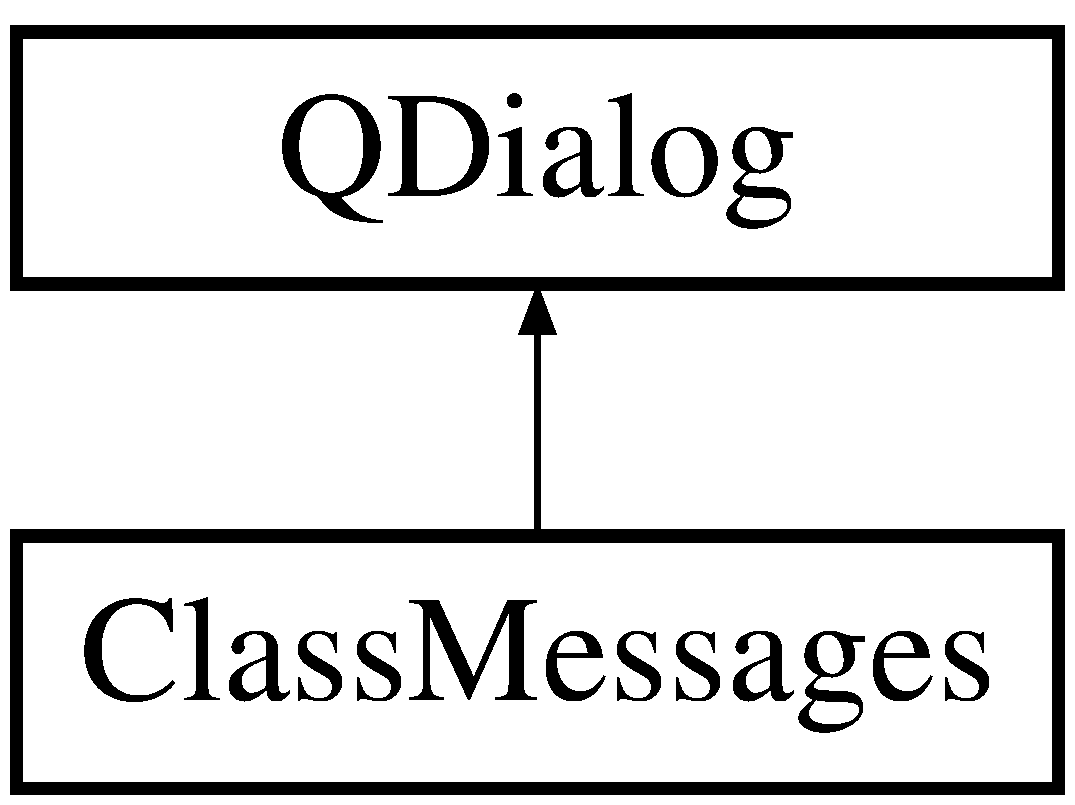
\includegraphics[height=2.000000cm]{class_class_messages}
\end{center}
\end{figure}
\subsection*{Signals}
\begin{DoxyCompactItemize}
\item 
void {\bfseries class\+Messages\+\_\+append\+Output} (\hyperlink{struct_message_classes}{Message\+Classes} message\+Classes)\hypertarget{class_class_messages_a0036b5812d6421f55ae892756219a680}{}\label{class_class_messages_a0036b5812d6421f55ae892756219a680}

\end{DoxyCompactItemize}
\subsection*{Public Member Functions}
\begin{DoxyCompactItemize}
\item 
{\bfseries Class\+Messages} (Q\+Widget $\ast$parent=0)\hypertarget{class_class_messages_a6eba787ba900af09b5a235826b6a748f}{}\label{class_class_messages_a6eba787ba900af09b5a235826b6a748f}

\item 
void {\bfseries class\+Messages\+\_\+change\+Load\+Vals} ()\hypertarget{class_class_messages_abde2b3837e9f0c1272008b2278746c7f}{}\label{class_class_messages_abde2b3837e9f0c1272008b2278746c7f}

\end{DoxyCompactItemize}


The documentation for this class was generated from the following files\+:\begin{DoxyCompactItemize}
\item 
/home/riley/work/fsw/src/isatgs/\+B\+A\+R\+Co\+Mm\+S/src/modules/\+B\+A\+R\+Co\+Mm\+S\+\_\+\+C\+F\+D\+P/classmessages.\+h\item 
/home/riley/work/fsw/src/isatgs/\+B\+A\+R\+Co\+Mm\+S/src/modules/\+B\+A\+R\+Co\+Mm\+S\+\_\+\+C\+F\+D\+P/classmessages.\+cpp\end{DoxyCompactItemize}

\hypertarget{class_color}{}\section{Color Class Reference}
\label{class_color}\index{Color@{Color}}
\subsection*{Public Member Functions}
\begin{DoxyCompactItemize}
\item 
{\bfseries Color} (std\+::string)\hypertarget{class_color_a6197debe831c5196234e088127bdb5dd}{}\label{class_color_a6197debe831c5196234e088127bdb5dd}

\item 
Q\+Brush {\bfseries color\+From\+Event} (std\+::string, bool opaque=true)\hypertarget{class_color_a537b119614ded99717825c126055ee1a}{}\label{class_color_a537b119614ded99717825c126055ee1a}

\item 
Q\+Brush {\bfseries color\+From\+String} (std\+::string, bool opaque=true)\hypertarget{class_color_a652fa6e29a5e4644e5768d2fa3878dc6}{}\label{class_color_a652fa6e29a5e4644e5768d2fa3878dc6}

\item 
Q\+Brush {\bfseries rand\+Color} ()\hypertarget{class_color_aa98c9fa2cc6ba5f40b32c7e6f0773e0c}{}\label{class_color_aa98c9fa2cc6ba5f40b32c7e6f0773e0c}

\item 
void {\bfseries load} (std\+::string)\hypertarget{class_color_a922d7d5a271232841fbf6f5c044579af}{}\label{class_color_a922d7d5a271232841fbf6f5c044579af}

\end{DoxyCompactItemize}


The documentation for this class was generated from the following files\+:\begin{DoxyCompactItemize}
\item 
/home/riley/work/fsw/src/isatgs/\+B\+A\+R\+Co\+Mm\+S/src/modules/\+B\+A\+R\+Co\+Mm\+S\+\_\+\+D\+I\+T\+L/bc\+\_\+ditl\+\_\+color\+Lib.\+h\item 
/home/riley/work/fsw/src/isatgs/\+B\+A\+R\+Co\+Mm\+S/src/modules/\+B\+A\+R\+Co\+Mm\+S\+\_\+\+D\+I\+T\+L/bc\+\_\+ditl\+\_\+color\+Lib.\+cpp\end{DoxyCompactItemize}

\hypertarget{classisat__utils_1_1_color_log_formatter}{}\section{isat\+\_\+utils\+:\+:Color\+Log\+Formatter Class Reference}
\label{classisat__utils_1_1_color_log_formatter}\index{isat\+\_\+utils\+::\+Color\+Log\+Formatter@{isat\+\_\+utils\+::\+Color\+Log\+Formatter}}
Inheritance diagram for isat\+\_\+utils\+:\+:Color\+Log\+Formatter\+:\begin{figure}[H]
\begin{center}
\leavevmode
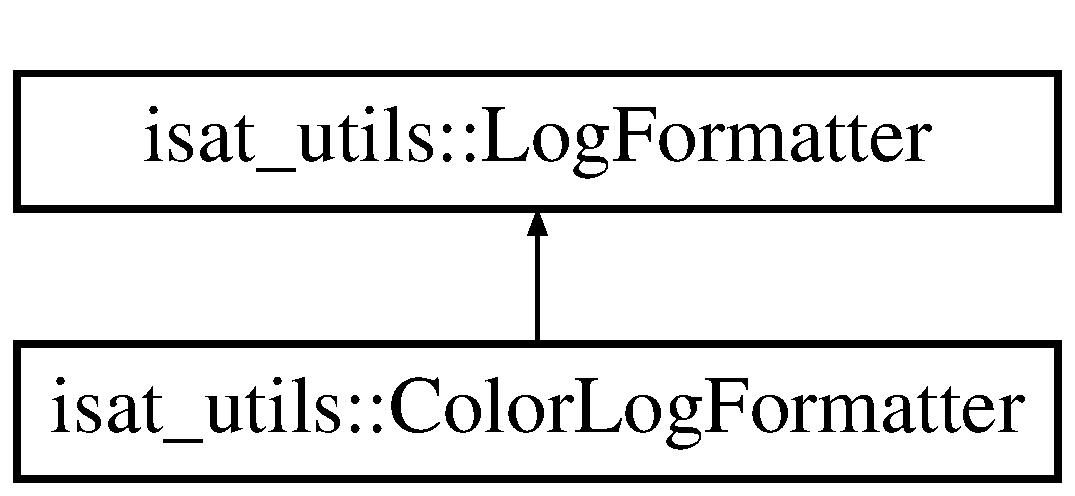
\includegraphics[height=2.000000cm]{classisat__utils_1_1_color_log_formatter}
\end{center}
\end{figure}
\subsection*{Public Member Functions}
\begin{DoxyCompactItemize}
\item 
std\+::string {\bfseries get\+Log\+Entry} (time\+\_\+t entry\+Time, Log\+Common\+::\+Log\+Level log\+Level, std\+::string logger\+Name, std\+::string message)\hypertarget{classisat__utils_1_1_color_log_formatter_aad19191600c36d45e035e7431b090f36}{}\label{classisat__utils_1_1_color_log_formatter_aad19191600c36d45e035e7431b090f36}

\item 
void {\bfseries enable\+Color} (bool flag)\hypertarget{classisat__utils_1_1_color_log_formatter_ae2ae478fa1b255d9757e67ad9d90a3af}{}\label{classisat__utils_1_1_color_log_formatter_ae2ae478fa1b255d9757e67ad9d90a3af}

\end{DoxyCompactItemize}
\subsection*{Protected Attributes}
\begin{DoxyCompactItemize}
\item 
bool {\bfseries color\+Enabled}\hypertarget{classisat__utils_1_1_color_log_formatter_a40f3f08435263cb5bd4cf50964054923}{}\label{classisat__utils_1_1_color_log_formatter_a40f3f08435263cb5bd4cf50964054923}

\item 
char const $\ast$ {\bfseries normal\+\_\+text}\hypertarget{classisat__utils_1_1_color_log_formatter_a90a60570f4fc2ad92187da6d4993009a}{}\label{classisat__utils_1_1_color_log_formatter_a90a60570f4fc2ad92187da6d4993009a}

\item 
char const $\ast$ {\bfseries bold\+\_\+text}\hypertarget{classisat__utils_1_1_color_log_formatter_adb67c7afbdf88cffcffb81c9df640258}{}\label{classisat__utils_1_1_color_log_formatter_adb67c7afbdf88cffcffb81c9df640258}

\item 
char const $\ast$ {\bfseries red\+\_\+text}\hypertarget{classisat__utils_1_1_color_log_formatter_a508657e3dce90ae0d6cc2b677b08e292}{}\label{classisat__utils_1_1_color_log_formatter_a508657e3dce90ae0d6cc2b677b08e292}

\item 
char const $\ast$ {\bfseries green\+\_\+text}\hypertarget{classisat__utils_1_1_color_log_formatter_af92416b4bd2b979350ba8bad5f76aa82}{}\label{classisat__utils_1_1_color_log_formatter_af92416b4bd2b979350ba8bad5f76aa82}

\item 
char const $\ast$ {\bfseries yellow\+\_\+text}\hypertarget{classisat__utils_1_1_color_log_formatter_a1ab6ac5eb3a696f681df63566465f559}{}\label{classisat__utils_1_1_color_log_formatter_a1ab6ac5eb3a696f681df63566465f559}

\item 
char const $\ast$ {\bfseries blue\+\_\+text}\hypertarget{classisat__utils_1_1_color_log_formatter_a4b57c2e3e6975ea1b009d8db01049570}{}\label{classisat__utils_1_1_color_log_formatter_a4b57c2e3e6975ea1b009d8db01049570}

\item 
char const $\ast$ {\bfseries magenta\+\_\+text}\hypertarget{classisat__utils_1_1_color_log_formatter_a0322afbae2627ecba34b25f53f900b1b}{}\label{classisat__utils_1_1_color_log_formatter_a0322afbae2627ecba34b25f53f900b1b}

\item 
char const $\ast$ {\bfseries cyan\+\_\+text}\hypertarget{classisat__utils_1_1_color_log_formatter_a748935b1b9a62986c1258a7d934c6ee1}{}\label{classisat__utils_1_1_color_log_formatter_a748935b1b9a62986c1258a7d934c6ee1}

\item 
char const $\ast$ {\bfseries white\+\_\+text}\hypertarget{classisat__utils_1_1_color_log_formatter_a4f9772879949d46d83b92674036a4165}{}\label{classisat__utils_1_1_color_log_formatter_a4f9772879949d46d83b92674036a4165}

\item 
char const $\ast$ {\bfseries defcolor}\hypertarget{classisat__utils_1_1_color_log_formatter_a8d271da6410a39fb1f43985a629ab4fe}{}\label{classisat__utils_1_1_color_log_formatter_a8d271da6410a39fb1f43985a629ab4fe}

\end{DoxyCompactItemize}


The documentation for this class was generated from the following files\+:\begin{DoxyCompactItemize}
\item 
/home/riley/work/fsw/src/isatgs/\+B\+A\+R\+Co\+Mm\+S/src/dependencies/utils/Color\+Log\+Formatter.\+h\item 
/home/riley/work/fsw/src/isatgs/\+B\+A\+R\+Co\+Mm\+S/src/dependencies/utils/Color\+Log\+Formatter.\+cpp\end{DoxyCompactItemize}

\hypertarget{classisat__trek_1_1_command_ids}{}\section{isat\+\_\+trek\+:\+:Command\+Ids Class Reference}
\label{classisat__trek_1_1_command_ids}\index{isat\+\_\+trek\+::\+Command\+Ids@{isat\+\_\+trek\+::\+Command\+Ids}}
\subsection*{Public Types}
\begin{DoxyCompactItemize}
\item 
enum {\bfseries Commands} \{ \\*
{\bfseries F\+S\+W\+\_\+\+C\+O\+N\+T\+R\+OL} = 1, 
{\bfseries T\+E\+L\+E\+M\+Q\+U\+E\+RY} = 5, 
{\bfseries C\+H\+A\+N\+G\+E\+M\+O\+DE} = 6, 
{\bfseries D\+E\+C\+O\+M\+\_\+\+C\+O\+M\+M\+IT} = 7, 
\\*
{\bfseries D\+E\+C\+O\+M\+\_\+\+E\+N\+A\+B\+LE} = 8
 \}\hypertarget{classisat__trek_1_1_command_ids_a8ddb80ea111233b76913d8125268c14a}{}\label{classisat__trek_1_1_command_ids_a8ddb80ea111233b76913d8125268c14a}

\end{DoxyCompactItemize}


The documentation for this class was generated from the following file\+:\begin{DoxyCompactItemize}
\item 
/home/riley/work/fsw/src/isatgs/\+B\+A\+R\+Co\+Mm\+S/src/dependencies/trek/Command\+Ids.\+h\end{DoxyCompactItemize}

\hypertarget{classisat__trek_1_1_comm_schedule___command}{}\section{isat\+\_\+trek\+:\+:Comm\+Schedule\+\_\+\+Command Class Reference}
\label{classisat__trek_1_1_comm_schedule___command}\index{isat\+\_\+trek\+::\+Comm\+Schedule\+\_\+\+Command@{isat\+\_\+trek\+::\+Comm\+Schedule\+\_\+\+Command}}


{\ttfamily \#include $<$Comm\+Schedule\+\_\+\+Command.\+h$>$}

Inheritance diagram for isat\+\_\+trek\+:\+:Comm\+Schedule\+\_\+\+Command\+:\begin{figure}[H]
\begin{center}
\leavevmode
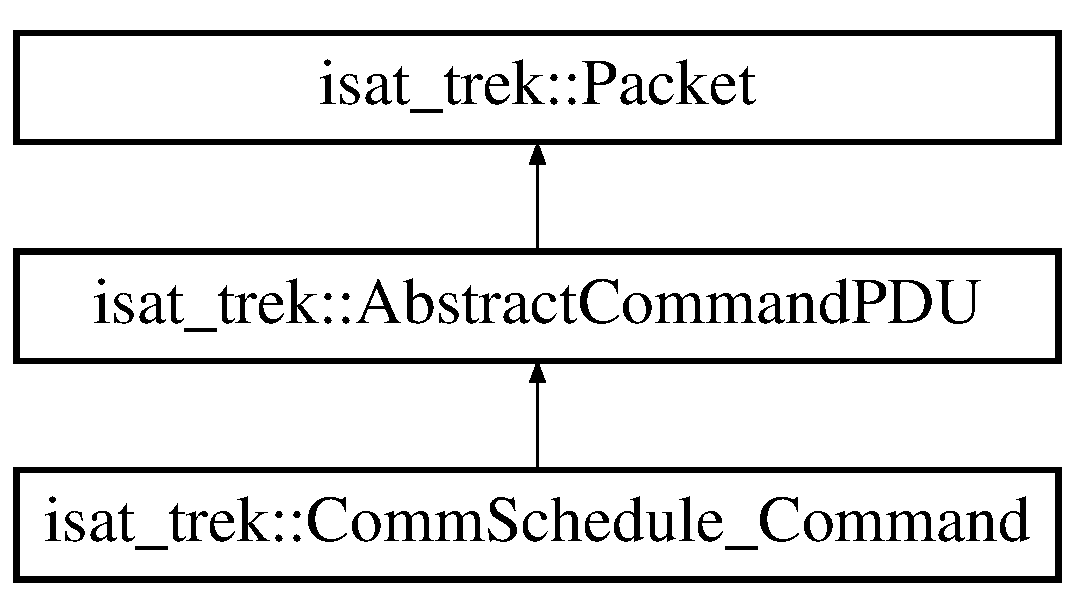
\includegraphics[height=3.000000cm]{classisat__trek_1_1_comm_schedule___command}
\end{center}
\end{figure}
\subsection*{Public Member Functions}
\begin{DoxyCompactItemize}
\item 
bool \hyperlink{classisat__trek_1_1_comm_schedule___command_a319741c38912475de0ded5d112fb8d5a}{from\+Bytes} (Byte\+Buffer \&buf)
\item 
bool \hyperlink{classisat__trek_1_1_comm_schedule___command_abb60891e0c1a5337b89262cb6ebe5439}{to\+Bytes} (Byte\+Buffer \&buf)
\end{DoxyCompactItemize}
\subsection*{Public Attributes}
\begin{DoxyCompactItemize}
\item 
int {\bfseries num\+Slots} = 0\hypertarget{classisat__trek_1_1_comm_schedule___command_a61d000b2dc1d4e82e8eb8c3fc8a2b0ad}{}\label{classisat__trek_1_1_comm_schedule___command_a61d000b2dc1d4e82e8eb8c3fc8a2b0ad}

\item 
int {\bfseries start\+Time1} = 0\hypertarget{classisat__trek_1_1_comm_schedule___command_a8d7e734093703c13828cab072f4adcd8}{}\label{classisat__trek_1_1_comm_schedule___command_a8d7e734093703c13828cab072f4adcd8}

\item 
int {\bfseries duration1} = 0\hypertarget{classisat__trek_1_1_comm_schedule___command_a0e425ffb9e0ac25963d0bf55d103ba5a}{}\label{classisat__trek_1_1_comm_schedule___command_a0e425ffb9e0ac25963d0bf55d103ba5a}

\item 
int {\bfseries data\+Rate1} = 0\hypertarget{classisat__trek_1_1_comm_schedule___command_af1d5b04d9d61ca853ae4fc6139dfeb06}{}\label{classisat__trek_1_1_comm_schedule___command_af1d5b04d9d61ca853ae4fc6139dfeb06}

\item 
int {\bfseries start\+Time2} = 0\hypertarget{classisat__trek_1_1_comm_schedule___command_a707181ec3f59bb6ae0f826f05753e747}{}\label{classisat__trek_1_1_comm_schedule___command_a707181ec3f59bb6ae0f826f05753e747}

\item 
int {\bfseries duration2} = 0\hypertarget{classisat__trek_1_1_comm_schedule___command_aaea85f88b7c92f0ec77814b574165e87}{}\label{classisat__trek_1_1_comm_schedule___command_aaea85f88b7c92f0ec77814b574165e87}

\item 
int {\bfseries data\+Rate2} = 0\hypertarget{classisat__trek_1_1_comm_schedule___command_a5b9d650cb616ae8922413f09bb4c8694}{}\label{classisat__trek_1_1_comm_schedule___command_a5b9d650cb616ae8922413f09bb4c8694}

\end{DoxyCompactItemize}


\subsection{Detailed Description}
X\+XX\+: Replace with real description in isat.\+pdu file. 

\subsection{Member Function Documentation}
\index{isat\+\_\+trek\+::\+Comm\+Schedule\+\_\+\+Command@{isat\+\_\+trek\+::\+Comm\+Schedule\+\_\+\+Command}!from\+Bytes@{from\+Bytes}}
\index{from\+Bytes@{from\+Bytes}!isat\+\_\+trek\+::\+Comm\+Schedule\+\_\+\+Command@{isat\+\_\+trek\+::\+Comm\+Schedule\+\_\+\+Command}}
\subsubsection[{\texorpdfstring{from\+Bytes(\+Byte\+Buffer \&buf)}{fromBytes(ByteBuffer &buf)}}]{\setlength{\rightskip}{0pt plus 5cm}bool isat\+\_\+trek\+::\+Comm\+Schedule\+\_\+\+Command\+::from\+Bytes (
\begin{DoxyParamCaption}
\item[{Byte\+Buffer \&}]{buf}
\end{DoxyParamCaption}
)\hspace{0.3cm}{\ttfamily [virtual]}}\hypertarget{classisat__trek_1_1_comm_schedule___command_a319741c38912475de0ded5d112fb8d5a}{}\label{classisat__trek_1_1_comm_schedule___command_a319741c38912475de0ded5d112fb8d5a}
Populate the header and command fields from the data in buf.

\begin{DoxyReturn}{Returns}
true if successful. 
\end{DoxyReturn}


Implements \hyperlink{classisat__trek_1_1_packet}{isat\+\_\+trek\+::\+Packet}.

\index{isat\+\_\+trek\+::\+Comm\+Schedule\+\_\+\+Command@{isat\+\_\+trek\+::\+Comm\+Schedule\+\_\+\+Command}!to\+Bytes@{to\+Bytes}}
\index{to\+Bytes@{to\+Bytes}!isat\+\_\+trek\+::\+Comm\+Schedule\+\_\+\+Command@{isat\+\_\+trek\+::\+Comm\+Schedule\+\_\+\+Command}}
\subsubsection[{\texorpdfstring{to\+Bytes(\+Byte\+Buffer \&buf)}{toBytes(ByteBuffer &buf)}}]{\setlength{\rightskip}{0pt plus 5cm}bool isat\+\_\+trek\+::\+Comm\+Schedule\+\_\+\+Command\+::to\+Bytes (
\begin{DoxyParamCaption}
\item[{Byte\+Buffer \&}]{buf}
\end{DoxyParamCaption}
)\hspace{0.3cm}{\ttfamily [virtual]}}\hypertarget{classisat__trek_1_1_comm_schedule___command_abb60891e0c1a5337b89262cb6ebe5439}{}\label{classisat__trek_1_1_comm_schedule___command_abb60891e0c1a5337b89262cb6ebe5439}
Create the binary representation of this instance in the specified buffer.

\begin{DoxyReturn}{Returns}
true if successful. 
\end{DoxyReturn}


Implements \hyperlink{classisat__trek_1_1_packet}{isat\+\_\+trek\+::\+Packet}.



The documentation for this class was generated from the following files\+:\begin{DoxyCompactItemize}
\item 
/home/riley/work/fsw/src/isatgs/\+B\+A\+R\+Co\+Mm\+S/src/dependencies/trek/command/Comm\+Schedule\+\_\+\+Command.\+h\item 
/home/riley/work/fsw/src/isatgs/\+B\+A\+R\+Co\+Mm\+S/src/dependencies/trek/command/Comm\+Schedule\+\_\+\+Command.\+cpp\end{DoxyCompactItemize}

\hypertarget{structisat__utils_1_1_conf_d_b_record}{}\section{isat\+\_\+utils\+:\+:Conf\+D\+B\+Record Struct Reference}
\label{structisat__utils_1_1_conf_d_b_record}\index{isat\+\_\+utils\+::\+Conf\+D\+B\+Record@{isat\+\_\+utils\+::\+Conf\+D\+B\+Record}}
\subsection*{Public Types}
\begin{DoxyCompactItemize}
\item 
enum {\bfseries Param\+Type} \{ {\bfseries B\+O\+OL}, 
{\bfseries I\+NT}, 
{\bfseries R\+E\+AL}, 
{\bfseries S\+T\+R\+I\+NG}
 \}\hypertarget{structisat__utils_1_1_conf_d_b_record_ad0e7abc3953ee6d56281554a176e704a}{}\label{structisat__utils_1_1_conf_d_b_record_ad0e7abc3953ee6d56281554a176e704a}

\end{DoxyCompactItemize}
\subsection*{Public Attributes}
\begin{DoxyCompactItemize}
\item 
\hyperlink{classisat__utils_1_1_string}{String} {\bfseries param\+Name}\hypertarget{structisat__utils_1_1_conf_d_b_record_a19383f4d9b04be00699573f37c377505}{}\label{structisat__utils_1_1_conf_d_b_record_a19383f4d9b04be00699573f37c377505}

\item 
Param\+Type {\bfseries param\+Type}\hypertarget{structisat__utils_1_1_conf_d_b_record_a8138b4ffdc45dece7d2640ed374c4fba}{}\label{structisat__utils_1_1_conf_d_b_record_a8138b4ffdc45dece7d2640ed374c4fba}

\item 
\hyperlink{classisat__utils_1_1_string}{String} {\bfseries description}\hypertarget{structisat__utils_1_1_conf_d_b_record_a2f2df7db2ce9408ea73e375c836f62e9}{}\label{structisat__utils_1_1_conf_d_b_record_a2f2df7db2ce9408ea73e375c836f62e9}

\item 
bool {\bfseries bool\+\_\+val}\hypertarget{structisat__utils_1_1_conf_d_b_record_a92408dad16fe9080359011e650768487}{}\label{structisat__utils_1_1_conf_d_b_record_a92408dad16fe9080359011e650768487}

\item 
long {\bfseries int\+\_\+val}\hypertarget{structisat__utils_1_1_conf_d_b_record_aeebd7aa509842f3ea933fd4ad145b2e8}{}\label{structisat__utils_1_1_conf_d_b_record_aeebd7aa509842f3ea933fd4ad145b2e8}

\item 
double {\bfseries real\+\_\+val}\hypertarget{structisat__utils_1_1_conf_d_b_record_a7dc605f5e51e57d918f9af5a43e76215}{}\label{structisat__utils_1_1_conf_d_b_record_a7dc605f5e51e57d918f9af5a43e76215}

\item 
\hyperlink{classisat__utils_1_1_string}{String} {\bfseries string\+\_\+val}\hypertarget{structisat__utils_1_1_conf_d_b_record_a74a7659f3f81e8ef6f8a4f0166679e59}{}\label{structisat__utils_1_1_conf_d_b_record_a74a7659f3f81e8ef6f8a4f0166679e59}

\end{DoxyCompactItemize}


The documentation for this struct was generated from the following file\+:\begin{DoxyCompactItemize}
\item 
/home/riley/work/fsw/src/isatgs/\+B\+A\+R\+Co\+Mm\+S/src/dependencies/utils/Conf\+D\+B\+Record.\+h\end{DoxyCompactItemize}

\hypertarget{classisat__utils_1_1_configuration_database}{}\section{isat\+\_\+utils\+:\+:Configuration\+Database Class Reference}
\label{classisat__utils_1_1_configuration_database}\index{isat\+\_\+utils\+::\+Configuration\+Database@{isat\+\_\+utils\+::\+Configuration\+Database}}


{\ttfamily \#include $<$Configuration\+Database.\+h$>$}

\subsection*{Public Member Functions}
\begin{DoxyCompactItemize}
\item 
bool \hyperlink{classisat__utils_1_1_configuration_database_afc0a79457de05c204ee8b8381646d5c6}{load} (\hyperlink{classisat__utils_1_1_file}{File} config\+Directory)
\item 
bool \hyperlink{classisat__utils_1_1_configuration_database_a33e1432c59eef927e6a7edcd94c6b7fe}{exists} (\hyperlink{classisat__utils_1_1_string}{String} param\+Name) const 
\item 
bool {\bfseries get\+Bool} (\hyperlink{classisat__utils_1_1_string}{String} param\+Name, bool default\+Value=false) const \hypertarget{classisat__utils_1_1_configuration_database_a97df465d1b0b77ff1d2f5b072cfd5a00}{}\label{classisat__utils_1_1_configuration_database_a97df465d1b0b77ff1d2f5b072cfd5a00}

\item 
long {\bfseries get\+Int} (\hyperlink{classisat__utils_1_1_string}{String} param\+Name, long default\+Value=0) const \hypertarget{classisat__utils_1_1_configuration_database_a263c773df281c83d8356b9eb54078a1f}{}\label{classisat__utils_1_1_configuration_database_a263c773df281c83d8356b9eb54078a1f}

\item 
double {\bfseries get\+Real} (\hyperlink{classisat__utils_1_1_string}{String} param\+Name, double default\+Value=0.\+0f) const \hypertarget{classisat__utils_1_1_configuration_database_ae2c0eb4bb1c6f6f414fb0cff369c22df}{}\label{classisat__utils_1_1_configuration_database_ae2c0eb4bb1c6f6f414fb0cff369c22df}

\item 
\hyperlink{classisat__utils_1_1_string}{String} \hyperlink{classisat__utils_1_1_configuration_database_a284544bd461710785a45f45144e83000}{get\+String} (\hyperlink{classisat__utils_1_1_string}{String} param\+Name, \hyperlink{classisat__utils_1_1_string}{String} default\+Value=\char`\"{}\char`\"{}) const 
\item 
void {\bfseries set\+Bool} (\hyperlink{classisat__utils_1_1_string}{String} param\+Name, bool value)\hypertarget{classisat__utils_1_1_configuration_database_a27569866fd1119f2cdb4071e3e3f30cb}{}\label{classisat__utils_1_1_configuration_database_a27569866fd1119f2cdb4071e3e3f30cb}

\item 
void {\bfseries set\+Int} (\hyperlink{classisat__utils_1_1_string}{String} param\+Name, long value)\hypertarget{classisat__utils_1_1_configuration_database_ab40a92697891b6330e59e17732d1a972}{}\label{classisat__utils_1_1_configuration_database_ab40a92697891b6330e59e17732d1a972}

\item 
void {\bfseries set\+Real} (\hyperlink{classisat__utils_1_1_string}{String} param\+Name, double value)\hypertarget{classisat__utils_1_1_configuration_database_a287e2182a22f187a808a2adbdb23b6a2}{}\label{classisat__utils_1_1_configuration_database_a287e2182a22f187a808a2adbdb23b6a2}

\item 
void {\bfseries set\+String} (\hyperlink{classisat__utils_1_1_string}{String} param\+Name, \hyperlink{classisat__utils_1_1_string}{String} value)\hypertarget{classisat__utils_1_1_configuration_database_a5292b904ee847227c62ea3c7d44d3ec7}{}\label{classisat__utils_1_1_configuration_database_a5292b904ee847227c62ea3c7d44d3ec7}

\item 
\hyperlink{classisat__utils_1_1_array_list}{Array\+List}$<$ \hyperlink{classisat__utils_1_1_string}{String} $>$ {\bfseries get\+Param\+Names} () const \hypertarget{classisat__utils_1_1_configuration_database_a60ece82305aad223f81b04cd730827f2}{}\label{classisat__utils_1_1_configuration_database_a60ece82305aad223f81b04cd730827f2}

\end{DoxyCompactItemize}
\subsection*{Static Public Member Functions}
\begin{DoxyCompactItemize}
\item 
static \hyperlink{classisat__utils_1_1_configuration_database}{Configuration\+Database} \& {\bfseries get\+Instance} ()\hypertarget{classisat__utils_1_1_configuration_database_ae0d9c0f437a4313de7a7845c98d0429f}{}\label{classisat__utils_1_1_configuration_database_ae0d9c0f437a4313de7a7845c98d0429f}

\end{DoxyCompactItemize}
\subsection*{Protected Member Functions}
\begin{DoxyCompactItemize}
\item 
bool {\bfseries parse\+Config} (json\+\_\+t $\ast$jsonobj)\hypertarget{classisat__utils_1_1_configuration_database_ae7f1dcdabef0a0d7b00739014daffbe4}{}\label{classisat__utils_1_1_configuration_database_ae7f1dcdabef0a0d7b00739014daffbe4}

\item 
bool {\bfseries find\+Param} (\hyperlink{classisat__utils_1_1_string}{String} param\+Name, int \&index) const \hypertarget{classisat__utils_1_1_configuration_database_ae2f3ff5553bef7ccf187d5088408088a}{}\label{classisat__utils_1_1_configuration_database_ae2f3ff5553bef7ccf187d5088408088a}

\end{DoxyCompactItemize}
\subsection*{Protected Attributes}
\begin{DoxyCompactItemize}
\item 
\hyperlink{classisat__utils_1_1_array_list}{Array\+List}$<$ \hyperlink{structisat__utils_1_1_conf_d_b_record}{Conf\+D\+B\+Record} $>$ {\bfseries symboltable}\hypertarget{classisat__utils_1_1_configuration_database_affd1efd34ebbec7f83375d4da911cfe5}{}\label{classisat__utils_1_1_configuration_database_affd1efd34ebbec7f83375d4da911cfe5}

\item 
\hyperlink{classisat__utils_1_1_logger}{Logger} {\bfseries logger}\hypertarget{classisat__utils_1_1_configuration_database_a09cb5bd5df5adbd1b55070a169d0b0d0}{}\label{classisat__utils_1_1_configuration_database_a09cb5bd5df5adbd1b55070a169d0b0d0}

\end{DoxyCompactItemize}


\subsection{Detailed Description}
The \hyperlink{classisat__utils_1_1_configuration_database}{Configuration\+Database} provides access to the contents of the configuration files in the config/ directory.

The load method should be called once to initialize the database, passing the location of the config/ directory. All configuration files with extension \char`\"{}.\+cfg\char`\"{} are passed to a lua interpreter instance for parsing / execution. 

\subsection{Member Function Documentation}
\index{isat\+\_\+utils\+::\+Configuration\+Database@{isat\+\_\+utils\+::\+Configuration\+Database}!exists@{exists}}
\index{exists@{exists}!isat\+\_\+utils\+::\+Configuration\+Database@{isat\+\_\+utils\+::\+Configuration\+Database}}
\subsubsection[{\texorpdfstring{exists(\+String param\+Name) const }{exists(String paramName) const }}]{\setlength{\rightskip}{0pt plus 5cm}bool isat\+\_\+utils\+::\+Configuration\+Database\+::exists (
\begin{DoxyParamCaption}
\item[{{\bf String}}]{param\+Name}
\end{DoxyParamCaption}
) const}\hypertarget{classisat__utils_1_1_configuration_database_a33e1432c59eef927e6a7edcd94c6b7fe}{}\label{classisat__utils_1_1_configuration_database_a33e1432c59eef927e6a7edcd94c6b7fe}
Determine if a parameter has a value in the database. \begin{DoxyReturn}{Returns}
true if parameter exists. 
\end{DoxyReturn}
\index{isat\+\_\+utils\+::\+Configuration\+Database@{isat\+\_\+utils\+::\+Configuration\+Database}!get\+String@{get\+String}}
\index{get\+String@{get\+String}!isat\+\_\+utils\+::\+Configuration\+Database@{isat\+\_\+utils\+::\+Configuration\+Database}}
\subsubsection[{\texorpdfstring{get\+String(\+String param\+Name, String default\+Value="""") const }{getString(String paramName, String defaultValue="") const }}]{\setlength{\rightskip}{0pt plus 5cm}{\bf String} isat\+\_\+utils\+::\+Configuration\+Database\+::get\+String (
\begin{DoxyParamCaption}
\item[{{\bf String}}]{param\+Name, }
\item[{{\bf String}}]{default\+Value = {\ttfamily \char`\"{}\char`\"{}}}
\end{DoxyParamCaption}
) const}\hypertarget{classisat__utils_1_1_configuration_database_a284544bd461710785a45f45144e83000}{}\label{classisat__utils_1_1_configuration_database_a284544bd461710785a45f45144e83000}
Get a string value from the configuration database. Callers should not free the returned pointer, the memory is managed by \hyperlink{classisat__utils_1_1_configuration_database}{Configuration\+Database}.

\begin{DoxyReturn}{Returns}

\end{DoxyReturn}
\index{isat\+\_\+utils\+::\+Configuration\+Database@{isat\+\_\+utils\+::\+Configuration\+Database}!load@{load}}
\index{load@{load}!isat\+\_\+utils\+::\+Configuration\+Database@{isat\+\_\+utils\+::\+Configuration\+Database}}
\subsubsection[{\texorpdfstring{load(\+File config\+Directory)}{load(File configDirectory)}}]{\setlength{\rightskip}{0pt plus 5cm}bool isat\+\_\+utils\+::\+Configuration\+Database\+::load (
\begin{DoxyParamCaption}
\item[{{\bf File}}]{config\+Directory}
\end{DoxyParamCaption}
)}\hypertarget{classisat__utils_1_1_configuration_database_afc0a79457de05c204ee8b8381646d5c6}{}\label{classisat__utils_1_1_configuration_database_afc0a79457de05c204ee8b8381646d5c6}
Load all configuration files located in directory config\+Path. \begin{DoxyReturn}{Returns}
true if load was successful. 
\end{DoxyReturn}


The documentation for this class was generated from the following files\+:\begin{DoxyCompactItemize}
\item 
/home/riley/work/fsw/src/isatgs/\+B\+A\+R\+Co\+Mm\+S/src/dependencies/utils/Configuration\+Database.\+h\item 
/home/riley/work/fsw/src/isatgs/\+B\+A\+R\+Co\+Mm\+S/src/dependencies/utils/Configuration\+Database.\+cpp\end{DoxyCompactItemize}

\hypertarget{classisat__utils_1_1_console_log}{}\section{isat\+\_\+utils\+:\+:Console\+Log Class Reference}
\label{classisat__utils_1_1_console_log}\index{isat\+\_\+utils\+::\+Console\+Log@{isat\+\_\+utils\+::\+Console\+Log}}
Inheritance diagram for isat\+\_\+utils\+:\+:Console\+Log\+:\begin{figure}[H]
\begin{center}
\leavevmode
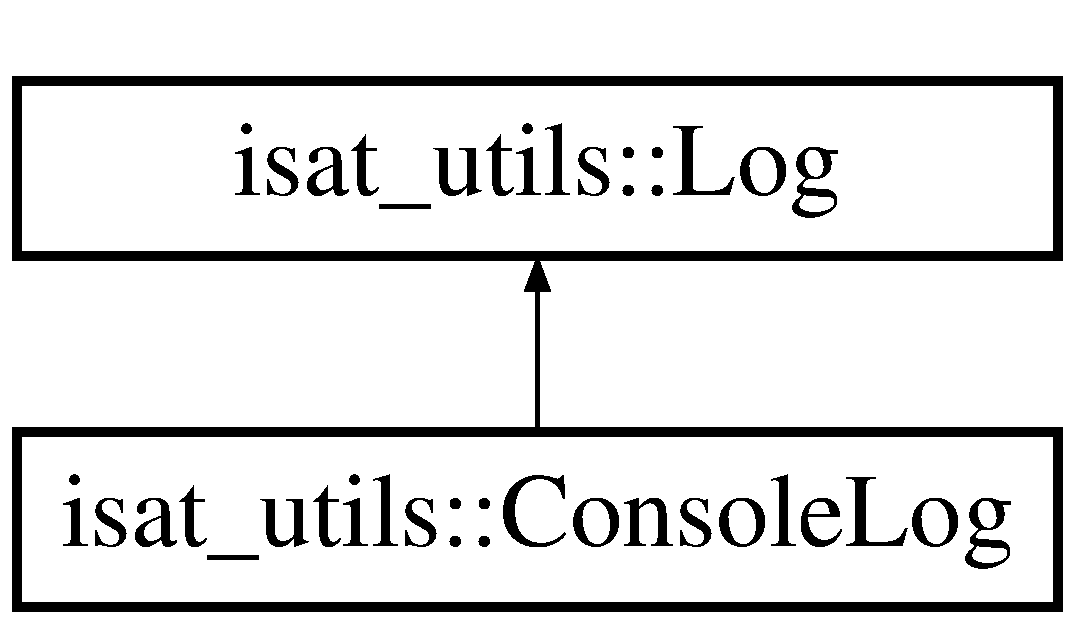
\includegraphics[height=2.000000cm]{classisat__utils_1_1_console_log}
\end{center}
\end{figure}
\subsection*{Public Member Functions}
\begin{DoxyCompactItemize}
\item 
bool {\bfseries write\+Entry} (Log\+Common\+::\+Log\+Level log\+Level, std\+::string logger\+Name, std\+::string message)\hypertarget{classisat__utils_1_1_console_log_a7b11508e2f1c5f6400aac4bf95a1757a}{}\label{classisat__utils_1_1_console_log_a7b11508e2f1c5f6400aac4bf95a1757a}

\end{DoxyCompactItemize}
\subsection*{Additional Inherited Members}


The documentation for this class was generated from the following files\+:\begin{DoxyCompactItemize}
\item 
/home/riley/work/fsw/src/isatgs/\+B\+A\+R\+Co\+Mm\+S/src/dependencies/utils/Console\+Log.\+h\item 
/home/riley/work/fsw/src/isatgs/\+B\+A\+R\+Co\+Mm\+S/src/dependencies/utils/Console\+Log.\+cpp\end{DoxyCompactItemize}

\hypertarget{classisat__utils_1_1_c_s_v_file}{}\section{isat\+\_\+utils\+:\+:C\+S\+V\+File Class Reference}
\label{classisat__utils_1_1_c_s_v_file}\index{isat\+\_\+utils\+::\+C\+S\+V\+File@{isat\+\_\+utils\+::\+C\+S\+V\+File}}


{\ttfamily \#include $<$C\+S\+V\+File.\+h$>$}

\subsection*{Public Member Functions}
\begin{DoxyCompactItemize}
\item 
bool {\bfseries open} (\hyperlink{classisat__utils_1_1_string}{String} filename)\hypertarget{classisat__utils_1_1_c_s_v_file_a991bc05745a6fe746c1a7da8b977db73}{}\label{classisat__utils_1_1_c_s_v_file_a991bc05745a6fe746c1a7da8b977db73}

\item 
bool \hyperlink{classisat__utils_1_1_c_s_v_file_af56251c0c090c574631137f7e424ae15}{get\+Line} ()
\item 
int {\bfseries get\+Int} (int column, int default\+Value)\hypertarget{classisat__utils_1_1_c_s_v_file_adf3fb9b1a9d6485a29fe130feab4cd29}{}\label{classisat__utils_1_1_c_s_v_file_adf3fb9b1a9d6485a29fe130feab4cd29}

\item 
double {\bfseries get\+Double} (int column, double default\+Value)\hypertarget{classisat__utils_1_1_c_s_v_file_a0da5fed556adaf00b7ebab7845206269}{}\label{classisat__utils_1_1_c_s_v_file_a0da5fed556adaf00b7ebab7845206269}

\item 
bool {\bfseries get\+Bool} (int column, bool default\+Value)\hypertarget{classisat__utils_1_1_c_s_v_file_a99e474ab83db4fa6b28121c33b6127af}{}\label{classisat__utils_1_1_c_s_v_file_a99e474ab83db4fa6b28121c33b6127af}

\item 
bool {\bfseries close} ()\hypertarget{classisat__utils_1_1_c_s_v_file_a5ebc0c933cee943ddc8e087752353cb2}{}\label{classisat__utils_1_1_c_s_v_file_a5ebc0c933cee943ddc8e087752353cb2}

\end{DoxyCompactItemize}


\subsection{Detailed Description}
Simple asbstraction to read and parse a comma separated value (C\+SV) file.

\hyperlink{classisat__utils_1_1_c_s_v_file}{C\+S\+V\+File} infile; infile.\+open(\char`\"{}foo.\+csv\char`\"{});

while(infile.\+get\+Line()) \{ int param1 = infile.\+get\+Int(26, 0); // Read column 26 as int, default value 0 double param2 = infile.\+get\+Double(14, 3.\+14); // Read column 14 as double, default value 3.\+14. \}

infile.\+close(); 

\subsection{Member Function Documentation}
\index{isat\+\_\+utils\+::\+C\+S\+V\+File@{isat\+\_\+utils\+::\+C\+S\+V\+File}!get\+Line@{get\+Line}}
\index{get\+Line@{get\+Line}!isat\+\_\+utils\+::\+C\+S\+V\+File@{isat\+\_\+utils\+::\+C\+S\+V\+File}}
\subsubsection[{\texorpdfstring{get\+Line()}{getLine()}}]{\setlength{\rightskip}{0pt plus 5cm}bool isat\+\_\+utils\+::\+C\+S\+V\+File\+::get\+Line (
\begin{DoxyParamCaption}
{}
\end{DoxyParamCaption}
)}\hypertarget{classisat__utils_1_1_c_s_v_file_af56251c0c090c574631137f7e424ae15}{}\label{classisat__utils_1_1_c_s_v_file_af56251c0c090c574631137f7e424ae15}
Reads the next line in the file and makes it available to be parsed by the get$\ast$() methods. \begin{DoxyReturn}{Returns}
false if no lines are left to read. 
\end{DoxyReturn}


The documentation for this class was generated from the following files\+:\begin{DoxyCompactItemize}
\item 
/home/riley/work/fsw/src/isatgs/\+B\+A\+R\+Co\+Mm\+S/src/dependencies/utils/C\+S\+V\+File.\+h\item 
/home/riley/work/fsw/src/isatgs/\+B\+A\+R\+Co\+Mm\+S/src/dependencies/utils/C\+S\+V\+File.\+cpp\end{DoxyCompactItemize}

\hypertarget{union_d_a_t_a___f_i_e_l_d}{}\section{D\+A\+T\+A\+\_\+\+F\+I\+E\+LD Union Reference}
\label{union_d_a_t_a___f_i_e_l_d}\index{D\+A\+T\+A\+\_\+\+F\+I\+E\+LD@{D\+A\+T\+A\+\_\+\+F\+I\+E\+LD}}
\subsection*{Public Attributes}
\begin{DoxyCompactItemize}
\item 
\hyperlink{struct_m_d}{MD} {\bfseries md}\hypertarget{union_d_a_t_a___f_i_e_l_d_a113e1d1025382e5f2b4867db45ffe83f}{}\label{union_d_a_t_a___f_i_e_l_d_a113e1d1025382e5f2b4867db45ffe83f}

\item 
\hyperlink{struct_f_d}{FD} {\bfseries fd}\hypertarget{union_d_a_t_a___f_i_e_l_d_a267cc025fb313995b4dd0136c13c93f7}{}\label{union_d_a_t_a___f_i_e_l_d_a267cc025fb313995b4dd0136c13c93f7}

\item 
\hyperlink{struct_e_o_h_f}{E\+O\+HF} {\bfseries eof}\hypertarget{union_d_a_t_a___f_i_e_l_d_a828a520d475b098bc9f3b241a467c537}{}\label{union_d_a_t_a___f_i_e_l_d_a828a520d475b098bc9f3b241a467c537}

\item 
\hyperlink{struct_f_i_n}{F\+IN} {\bfseries fin}\hypertarget{union_d_a_t_a___f_i_e_l_d_a1cb02724adbc22940dd14ff3f416cfb1}{}\label{union_d_a_t_a___f_i_e_l_d_a1cb02724adbc22940dd14ff3f416cfb1}

\item 
\hyperlink{struct_a_c_k}{A\+CK} {\bfseries ack}\hypertarget{union_d_a_t_a___f_i_e_l_d_ac9a6232da12140a2d22cefeb7a244a65}{}\label{union_d_a_t_a___f_i_e_l_d_ac9a6232da12140a2d22cefeb7a244a65}

\item 
\hyperlink{struct_n_a_k}{N\+AK} {\bfseries nak}\hypertarget{union_d_a_t_a___f_i_e_l_d_aa4ac035bac0b657c409fdf9bd5413b8e}{}\label{union_d_a_t_a___f_i_e_l_d_aa4ac035bac0b657c409fdf9bd5413b8e}

\end{DoxyCompactItemize}


The documentation for this union was generated from the following file\+:\begin{DoxyCompactItemize}
\item 
/home/riley/work/fsw/src/isatgs/\+B\+A\+R\+Co\+Mm\+S/src/dependencies/\+C\+F\+D\+P/\+P\+R\+I/structures.\+h\end{DoxyCompactItemize}

\hypertarget{classisat__trek_1_1_decom___commit___command}{}\section{isat\+\_\+trek\+:\+:Decom\+\_\+\+Commit\+\_\+\+Command Class Reference}
\label{classisat__trek_1_1_decom___commit___command}\index{isat\+\_\+trek\+::\+Decom\+\_\+\+Commit\+\_\+\+Command@{isat\+\_\+trek\+::\+Decom\+\_\+\+Commit\+\_\+\+Command}}


{\ttfamily \#include $<$Decom\+\_\+\+Commit\+\_\+\+Command.\+h$>$}

Inheritance diagram for isat\+\_\+trek\+:\+:Decom\+\_\+\+Commit\+\_\+\+Command\+:\begin{figure}[H]
\begin{center}
\leavevmode
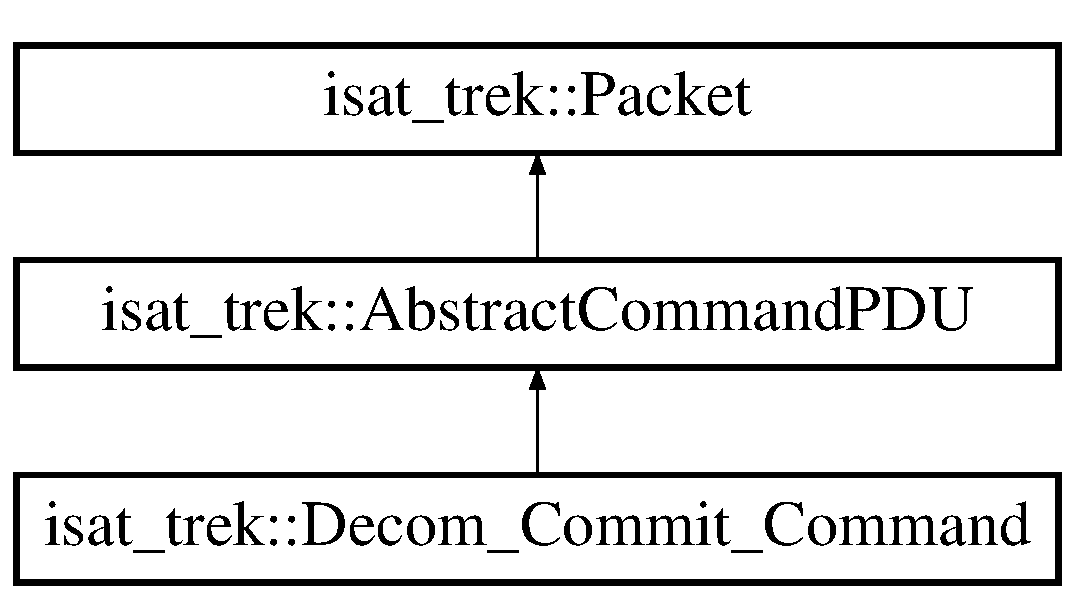
\includegraphics[height=3.000000cm]{classisat__trek_1_1_decom___commit___command}
\end{center}
\end{figure}
\subsection*{Public Member Functions}
\begin{DoxyCompactItemize}
\item 
bool \hyperlink{classisat__trek_1_1_decom___commit___command_a22eb09166f279f873a8f9fb7d82137c9}{from\+Bytes} (Byte\+Buffer \&buf)
\item 
bool \hyperlink{classisat__trek_1_1_decom___commit___command_a5e07be18b1edb1669e06bca197f3376e}{to\+Bytes} (Byte\+Buffer \&buf)
\end{DoxyCompactItemize}
\subsection*{Additional Inherited Members}


\subsection{Detailed Description}
X\+XX\+: Replace with real description in isat.\+pdu file. 

\subsection{Member Function Documentation}
\index{isat\+\_\+trek\+::\+Decom\+\_\+\+Commit\+\_\+\+Command@{isat\+\_\+trek\+::\+Decom\+\_\+\+Commit\+\_\+\+Command}!from\+Bytes@{from\+Bytes}}
\index{from\+Bytes@{from\+Bytes}!isat\+\_\+trek\+::\+Decom\+\_\+\+Commit\+\_\+\+Command@{isat\+\_\+trek\+::\+Decom\+\_\+\+Commit\+\_\+\+Command}}
\subsubsection[{\texorpdfstring{from\+Bytes(\+Byte\+Buffer \&buf)}{fromBytes(ByteBuffer &buf)}}]{\setlength{\rightskip}{0pt plus 5cm}bool isat\+\_\+trek\+::\+Decom\+\_\+\+Commit\+\_\+\+Command\+::from\+Bytes (
\begin{DoxyParamCaption}
\item[{Byte\+Buffer \&}]{buf}
\end{DoxyParamCaption}
)\hspace{0.3cm}{\ttfamily [virtual]}}\hypertarget{classisat__trek_1_1_decom___commit___command_a22eb09166f279f873a8f9fb7d82137c9}{}\label{classisat__trek_1_1_decom___commit___command_a22eb09166f279f873a8f9fb7d82137c9}
Populate the header and command fields from the data in buf.

\begin{DoxyReturn}{Returns}
true if successful. 
\end{DoxyReturn}


Implements \hyperlink{classisat__trek_1_1_packet}{isat\+\_\+trek\+::\+Packet}.

\index{isat\+\_\+trek\+::\+Decom\+\_\+\+Commit\+\_\+\+Command@{isat\+\_\+trek\+::\+Decom\+\_\+\+Commit\+\_\+\+Command}!to\+Bytes@{to\+Bytes}}
\index{to\+Bytes@{to\+Bytes}!isat\+\_\+trek\+::\+Decom\+\_\+\+Commit\+\_\+\+Command@{isat\+\_\+trek\+::\+Decom\+\_\+\+Commit\+\_\+\+Command}}
\subsubsection[{\texorpdfstring{to\+Bytes(\+Byte\+Buffer \&buf)}{toBytes(ByteBuffer &buf)}}]{\setlength{\rightskip}{0pt plus 5cm}bool isat\+\_\+trek\+::\+Decom\+\_\+\+Commit\+\_\+\+Command\+::to\+Bytes (
\begin{DoxyParamCaption}
\item[{Byte\+Buffer \&}]{buf}
\end{DoxyParamCaption}
)\hspace{0.3cm}{\ttfamily [virtual]}}\hypertarget{classisat__trek_1_1_decom___commit___command_a5e07be18b1edb1669e06bca197f3376e}{}\label{classisat__trek_1_1_decom___commit___command_a5e07be18b1edb1669e06bca197f3376e}
Create the binary representation of this instance in the specified buffer.

\begin{DoxyReturn}{Returns}
true if successful. 
\end{DoxyReturn}


Implements \hyperlink{classisat__trek_1_1_packet}{isat\+\_\+trek\+::\+Packet}.



The documentation for this class was generated from the following files\+:\begin{DoxyCompactItemize}
\item 
/home/riley/work/fsw/src/isatgs/\+B\+A\+R\+Co\+Mm\+S/src/dependencies/trek/command/Decom\+\_\+\+Commit\+\_\+\+Command.\+h\item 
/home/riley/work/fsw/src/isatgs/\+B\+A\+R\+Co\+Mm\+S/src/dependencies/trek/command/Decom\+\_\+\+Commit\+\_\+\+Command.\+cpp\end{DoxyCompactItemize}

\hypertarget{classisat__trek_1_1_decom___enable___command}{}\section{isat\+\_\+trek\+:\+:Decom\+\_\+\+Enable\+\_\+\+Command Class Reference}
\label{classisat__trek_1_1_decom___enable___command}\index{isat\+\_\+trek\+::\+Decom\+\_\+\+Enable\+\_\+\+Command@{isat\+\_\+trek\+::\+Decom\+\_\+\+Enable\+\_\+\+Command}}


{\ttfamily \#include $<$Decom\+\_\+\+Enable\+\_\+\+Command.\+h$>$}

Inheritance diagram for isat\+\_\+trek\+:\+:Decom\+\_\+\+Enable\+\_\+\+Command\+:\begin{figure}[H]
\begin{center}
\leavevmode
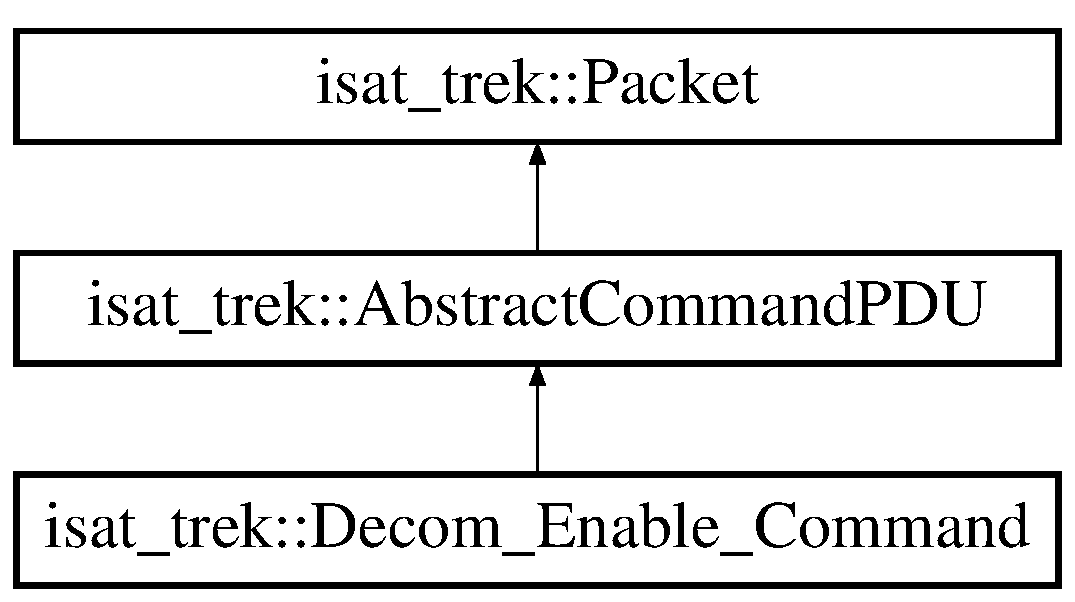
\includegraphics[height=3.000000cm]{classisat__trek_1_1_decom___enable___command}
\end{center}
\end{figure}
\subsection*{Public Member Functions}
\begin{DoxyCompactItemize}
\item 
bool \hyperlink{classisat__trek_1_1_decom___enable___command_a5e1c160cf9cd7f385b1bcb149c7663e4}{from\+Bytes} (Byte\+Buffer \&buf)
\item 
bool \hyperlink{classisat__trek_1_1_decom___enable___command_acf7e7fd30cd0fe89ceac444909baf115}{to\+Bytes} (Byte\+Buffer \&buf)
\end{DoxyCompactItemize}
\subsection*{Additional Inherited Members}


\subsection{Detailed Description}
X\+XX\+: Replace with real description in isat.\+pdu file. 

\subsection{Member Function Documentation}
\index{isat\+\_\+trek\+::\+Decom\+\_\+\+Enable\+\_\+\+Command@{isat\+\_\+trek\+::\+Decom\+\_\+\+Enable\+\_\+\+Command}!from\+Bytes@{from\+Bytes}}
\index{from\+Bytes@{from\+Bytes}!isat\+\_\+trek\+::\+Decom\+\_\+\+Enable\+\_\+\+Command@{isat\+\_\+trek\+::\+Decom\+\_\+\+Enable\+\_\+\+Command}}
\subsubsection[{\texorpdfstring{from\+Bytes(\+Byte\+Buffer \&buf)}{fromBytes(ByteBuffer &buf)}}]{\setlength{\rightskip}{0pt plus 5cm}bool isat\+\_\+trek\+::\+Decom\+\_\+\+Enable\+\_\+\+Command\+::from\+Bytes (
\begin{DoxyParamCaption}
\item[{Byte\+Buffer \&}]{buf}
\end{DoxyParamCaption}
)\hspace{0.3cm}{\ttfamily [virtual]}}\hypertarget{classisat__trek_1_1_decom___enable___command_a5e1c160cf9cd7f385b1bcb149c7663e4}{}\label{classisat__trek_1_1_decom___enable___command_a5e1c160cf9cd7f385b1bcb149c7663e4}
Populate the header and command fields from the data in buf.

\begin{DoxyReturn}{Returns}
true if successful. 
\end{DoxyReturn}


Implements \hyperlink{classisat__trek_1_1_packet}{isat\+\_\+trek\+::\+Packet}.

\index{isat\+\_\+trek\+::\+Decom\+\_\+\+Enable\+\_\+\+Command@{isat\+\_\+trek\+::\+Decom\+\_\+\+Enable\+\_\+\+Command}!to\+Bytes@{to\+Bytes}}
\index{to\+Bytes@{to\+Bytes}!isat\+\_\+trek\+::\+Decom\+\_\+\+Enable\+\_\+\+Command@{isat\+\_\+trek\+::\+Decom\+\_\+\+Enable\+\_\+\+Command}}
\subsubsection[{\texorpdfstring{to\+Bytes(\+Byte\+Buffer \&buf)}{toBytes(ByteBuffer &buf)}}]{\setlength{\rightskip}{0pt plus 5cm}bool isat\+\_\+trek\+::\+Decom\+\_\+\+Enable\+\_\+\+Command\+::to\+Bytes (
\begin{DoxyParamCaption}
\item[{Byte\+Buffer \&}]{buf}
\end{DoxyParamCaption}
)\hspace{0.3cm}{\ttfamily [virtual]}}\hypertarget{classisat__trek_1_1_decom___enable___command_acf7e7fd30cd0fe89ceac444909baf115}{}\label{classisat__trek_1_1_decom___enable___command_acf7e7fd30cd0fe89ceac444909baf115}
Create the binary representation of this instance in the specified buffer.

\begin{DoxyReturn}{Returns}
true if successful. 
\end{DoxyReturn}


Implements \hyperlink{classisat__trek_1_1_packet}{isat\+\_\+trek\+::\+Packet}.



The documentation for this class was generated from the following files\+:\begin{DoxyCompactItemize}
\item 
/home/riley/work/fsw/src/isatgs/\+B\+A\+R\+Co\+Mm\+S/src/dependencies/trek/command/Decom\+\_\+\+Enable\+\_\+\+Command.\+h\item 
/home/riley/work/fsw/src/isatgs/\+B\+A\+R\+Co\+Mm\+S/src/dependencies/trek/command/Decom\+\_\+\+Enable\+\_\+\+Command.\+cpp\end{DoxyCompactItemize}

\hypertarget{classisat__utils_1_1_default_log_filter}{}\section{isat\+\_\+utils\+:\+:Default\+Log\+Filter Class Reference}
\label{classisat__utils_1_1_default_log_filter}\index{isat\+\_\+utils\+::\+Default\+Log\+Filter@{isat\+\_\+utils\+::\+Default\+Log\+Filter}}
Inheritance diagram for isat\+\_\+utils\+:\+:Default\+Log\+Filter\+:\begin{figure}[H]
\begin{center}
\leavevmode
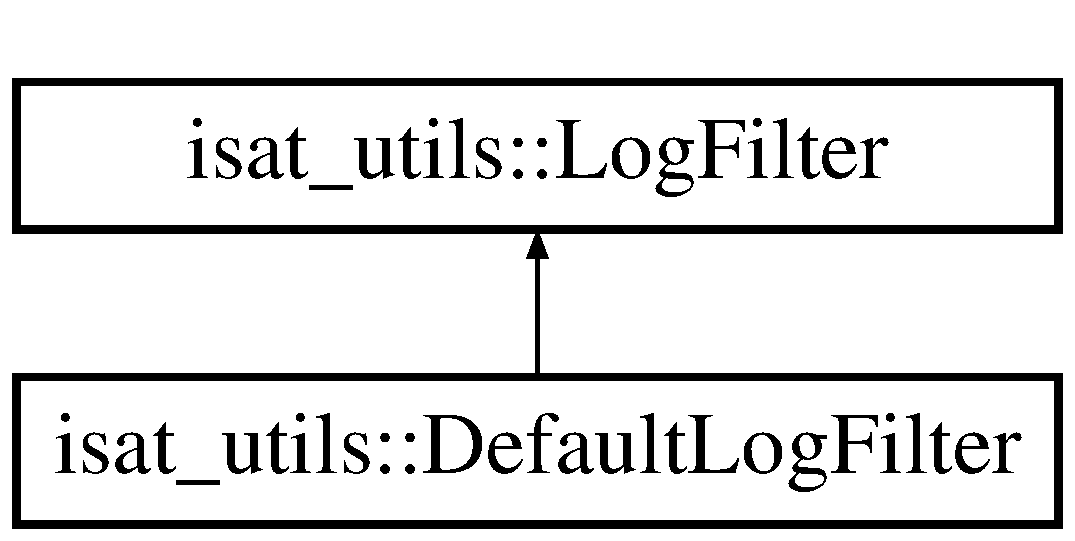
\includegraphics[height=2.000000cm]{classisat__utils_1_1_default_log_filter}
\end{center}
\end{figure}
\subsection*{Public Member Functions}
\begin{DoxyCompactItemize}
\item 
void {\bfseries set\+Minimum\+Log\+Level} (Log\+Common\+::\+Log\+Level min\+Log\+Level)\hypertarget{classisat__utils_1_1_default_log_filter_a7c739de097c001abd976172df5e032f3}{}\label{classisat__utils_1_1_default_log_filter_a7c739de097c001abd976172df5e032f3}

\item 
bool {\bfseries check\+Entry} (Log\+Common\+::\+Log\+Level log\+Level, std\+::string logger\+Name, std\+::string message)\hypertarget{classisat__utils_1_1_default_log_filter_ab2f4283bc320cd69c9316052f1dedc77}{}\label{classisat__utils_1_1_default_log_filter_ab2f4283bc320cd69c9316052f1dedc77}

\end{DoxyCompactItemize}
\subsection*{Protected Attributes}
\begin{DoxyCompactItemize}
\item 
Log\+Common\+::\+Log\+Level {\bfseries min\+Log\+Level}\hypertarget{classisat__utils_1_1_default_log_filter_ac63a7dfcd5dcc6f182998f4ce967f4d5}{}\label{classisat__utils_1_1_default_log_filter_ac63a7dfcd5dcc6f182998f4ce967f4d5}

\end{DoxyCompactItemize}


The documentation for this class was generated from the following files\+:\begin{DoxyCompactItemize}
\item 
/home/riley/work/fsw/src/isatgs/\+B\+A\+R\+Co\+Mm\+S/src/dependencies/utils/Default\+Log\+Filter.\+h\item 
/home/riley/work/fsw/src/isatgs/\+B\+A\+R\+Co\+Mm\+S/src/dependencies/utils/Default\+Log\+Filter.\+cpp\end{DoxyCompactItemize}

\hypertarget{classisat__trek_1_1_downlink_buffer___command}{}\section{isat\+\_\+trek\+:\+:Downlink\+Buffer\+\_\+\+Command Class Reference}
\label{classisat__trek_1_1_downlink_buffer___command}\index{isat\+\_\+trek\+::\+Downlink\+Buffer\+\_\+\+Command@{isat\+\_\+trek\+::\+Downlink\+Buffer\+\_\+\+Command}}


{\ttfamily \#include $<$Downlink\+Buffer\+\_\+\+Command.\+h$>$}

Inheritance diagram for isat\+\_\+trek\+:\+:Downlink\+Buffer\+\_\+\+Command\+:\begin{figure}[H]
\begin{center}
\leavevmode
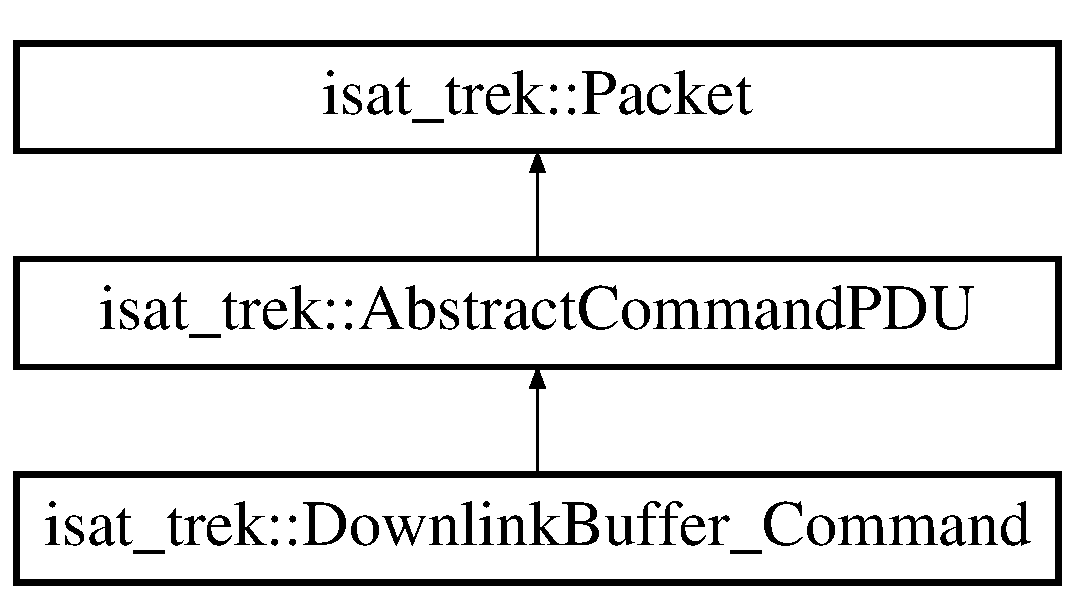
\includegraphics[height=3.000000cm]{classisat__trek_1_1_downlink_buffer___command}
\end{center}
\end{figure}
\subsection*{Public Member Functions}
\begin{DoxyCompactItemize}
\item 
bool \hyperlink{classisat__trek_1_1_downlink_buffer___command_a5cfd8df9c46fac235fcd9b50f4c5053b}{from\+Bytes} (Byte\+Buffer \&buf)
\item 
bool \hyperlink{classisat__trek_1_1_downlink_buffer___command_ae4b93f851e4424c43ba4b51c3cf32e40}{to\+Bytes} (Byte\+Buffer \&buf)
\end{DoxyCompactItemize}
\subsection*{Additional Inherited Members}


\subsection{Detailed Description}
X\+XX\+: Replace with real description in isat.\+pdu file. 

\subsection{Member Function Documentation}
\index{isat\+\_\+trek\+::\+Downlink\+Buffer\+\_\+\+Command@{isat\+\_\+trek\+::\+Downlink\+Buffer\+\_\+\+Command}!from\+Bytes@{from\+Bytes}}
\index{from\+Bytes@{from\+Bytes}!isat\+\_\+trek\+::\+Downlink\+Buffer\+\_\+\+Command@{isat\+\_\+trek\+::\+Downlink\+Buffer\+\_\+\+Command}}
\subsubsection[{\texorpdfstring{from\+Bytes(\+Byte\+Buffer \&buf)}{fromBytes(ByteBuffer &buf)}}]{\setlength{\rightskip}{0pt plus 5cm}bool isat\+\_\+trek\+::\+Downlink\+Buffer\+\_\+\+Command\+::from\+Bytes (
\begin{DoxyParamCaption}
\item[{Byte\+Buffer \&}]{buf}
\end{DoxyParamCaption}
)\hspace{0.3cm}{\ttfamily [virtual]}}\hypertarget{classisat__trek_1_1_downlink_buffer___command_a5cfd8df9c46fac235fcd9b50f4c5053b}{}\label{classisat__trek_1_1_downlink_buffer___command_a5cfd8df9c46fac235fcd9b50f4c5053b}
Populate the header and command fields from the data in buf.

\begin{DoxyReturn}{Returns}
true if successful. 
\end{DoxyReturn}


Implements \hyperlink{classisat__trek_1_1_packet}{isat\+\_\+trek\+::\+Packet}.

\index{isat\+\_\+trek\+::\+Downlink\+Buffer\+\_\+\+Command@{isat\+\_\+trek\+::\+Downlink\+Buffer\+\_\+\+Command}!to\+Bytes@{to\+Bytes}}
\index{to\+Bytes@{to\+Bytes}!isat\+\_\+trek\+::\+Downlink\+Buffer\+\_\+\+Command@{isat\+\_\+trek\+::\+Downlink\+Buffer\+\_\+\+Command}}
\subsubsection[{\texorpdfstring{to\+Bytes(\+Byte\+Buffer \&buf)}{toBytes(ByteBuffer &buf)}}]{\setlength{\rightskip}{0pt plus 5cm}bool isat\+\_\+trek\+::\+Downlink\+Buffer\+\_\+\+Command\+::to\+Bytes (
\begin{DoxyParamCaption}
\item[{Byte\+Buffer \&}]{buf}
\end{DoxyParamCaption}
)\hspace{0.3cm}{\ttfamily [virtual]}}\hypertarget{classisat__trek_1_1_downlink_buffer___command_ae4b93f851e4424c43ba4b51c3cf32e40}{}\label{classisat__trek_1_1_downlink_buffer___command_ae4b93f851e4424c43ba4b51c3cf32e40}
Create the binary representation of this instance in the specified buffer.

\begin{DoxyReturn}{Returns}
true if successful. 
\end{DoxyReturn}


Implements \hyperlink{classisat__trek_1_1_packet}{isat\+\_\+trek\+::\+Packet}.



The documentation for this class was generated from the following files\+:\begin{DoxyCompactItemize}
\item 
/home/riley/work/fsw/src/isatgs/\+B\+A\+R\+Co\+Mm\+S/src/dependencies/trek/command/Downlink\+Buffer\+\_\+\+Command.\+h\item 
/home/riley/work/fsw/src/isatgs/\+B\+A\+R\+Co\+Mm\+S/src/dependencies/trek/command/Downlink\+Buffer\+\_\+\+Command.\+cpp\end{DoxyCompactItemize}

\hypertarget{classtinyxml2_1_1_dyn_array}{}\section{tinyxml2\+:\+:Dyn\+Array$<$ T, I\+N\+IT $>$ Class Template Reference}
\label{classtinyxml2_1_1_dyn_array}\index{tinyxml2\+::\+Dyn\+Array$<$ T, I\+N\+I\+T $>$@{tinyxml2\+::\+Dyn\+Array$<$ T, I\+N\+I\+T $>$}}
\subsection*{Public Member Functions}
\begin{DoxyCompactItemize}
\item 
void {\bfseries Push} (T t)\hypertarget{classtinyxml2_1_1_dyn_array_a498de53808ba0151fef54ea10bf51050}{}\label{classtinyxml2_1_1_dyn_array_a498de53808ba0151fef54ea10bf51050}

\item 
T $\ast$ {\bfseries Push\+Arr} (int count)\hypertarget{classtinyxml2_1_1_dyn_array_aa3c360d40addc3b05121da9f60a01b4d}{}\label{classtinyxml2_1_1_dyn_array_aa3c360d40addc3b05121da9f60a01b4d}

\item 
T {\bfseries Pop} ()\hypertarget{classtinyxml2_1_1_dyn_array_a2281e3342bc235bf391a67e362c75866}{}\label{classtinyxml2_1_1_dyn_array_a2281e3342bc235bf391a67e362c75866}

\item 
void {\bfseries Pop\+Arr} (int count)\hypertarget{classtinyxml2_1_1_dyn_array_ab45c0836d8c0260a5b9eda7da80de71c}{}\label{classtinyxml2_1_1_dyn_array_ab45c0836d8c0260a5b9eda7da80de71c}

\item 
bool {\bfseries Empty} () const \hypertarget{classtinyxml2_1_1_dyn_array_a080dc4dc68713964bb17745d4c833158}{}\label{classtinyxml2_1_1_dyn_array_a080dc4dc68713964bb17745d4c833158}

\item 
T \& {\bfseries operator\mbox{[}$\,$\mbox{]}} (int i)\hypertarget{classtinyxml2_1_1_dyn_array_a775a6ab4d41f0eb15bdd863d408dd58f}{}\label{classtinyxml2_1_1_dyn_array_a775a6ab4d41f0eb15bdd863d408dd58f}

\item 
const T \& {\bfseries operator\mbox{[}$\,$\mbox{]}} (int i) const \hypertarget{classtinyxml2_1_1_dyn_array_a1f4874c2608cbd68be1627fca9efd820}{}\label{classtinyxml2_1_1_dyn_array_a1f4874c2608cbd68be1627fca9efd820}

\item 
int {\bfseries Size} () const \hypertarget{classtinyxml2_1_1_dyn_array_a1299b257b62ea6b4983c488867f219b0}{}\label{classtinyxml2_1_1_dyn_array_a1299b257b62ea6b4983c488867f219b0}

\item 
int {\bfseries Capacity} () const \hypertarget{classtinyxml2_1_1_dyn_array_a8edbe90ed53b2e46b1b5cf53b261e4e7}{}\label{classtinyxml2_1_1_dyn_array_a8edbe90ed53b2e46b1b5cf53b261e4e7}

\item 
const T $\ast$ {\bfseries Mem} () const \hypertarget{classtinyxml2_1_1_dyn_array_a1f39330daeb97d3d1dc3fc12dcf7ac67}{}\label{classtinyxml2_1_1_dyn_array_a1f39330daeb97d3d1dc3fc12dcf7ac67}

\item 
T $\ast$ {\bfseries Mem} ()\hypertarget{classtinyxml2_1_1_dyn_array_a0e0d60b399d54fad5b33d5008bc59c8e}{}\label{classtinyxml2_1_1_dyn_array_a0e0d60b399d54fad5b33d5008bc59c8e}

\end{DoxyCompactItemize}


The documentation for this class was generated from the following file\+:\begin{DoxyCompactItemize}
\item 
/home/riley/work/fsw/src/isatgs/\+B\+A\+R\+Co\+Mm\+S/src/dependencies/utils/tinyxml2.\+h\end{DoxyCompactItemize}

\hypertarget{classisat__net_1_1_end_point}{}\section{isat\+\_\+net\+:\+:End\+Point Class Reference}
\label{classisat__net_1_1_end_point}\index{isat\+\_\+net\+::\+End\+Point@{isat\+\_\+net\+::\+End\+Point}}


{\ttfamily \#include $<$End\+Point.\+h$>$}

\subsection*{Public Member Functions}
\begin{DoxyCompactItemize}
\item 
{\bfseries End\+Point} (\hyperlink{classisat__utils_1_1_string}{String} host, int port=0)\hypertarget{classisat__net_1_1_end_point_a01c39ec95d01dee0b26b62bd252bfdc0}{}\label{classisat__net_1_1_end_point_a01c39ec95d01dee0b26b62bd252bfdc0}

\item 
{\bfseries End\+Point} (int port)\hypertarget{classisat__net_1_1_end_point_af00285be71b71cb6dd93cf09ab54fd39}{}\label{classisat__net_1_1_end_point_af00285be71b71cb6dd93cf09ab54fd39}

\item 
bool \hyperlink{classisat__net_1_1_end_point_afbbe067c11aab5bb65de09aca5c4aa3a}{set\+Host} (\hyperlink{classisat__utils_1_1_string}{String} address)
\item 
\hyperlink{classisat__utils_1_1_string}{String} {\bfseries get\+Host} () const \hypertarget{classisat__net_1_1_end_point_a4e9cfb1be0f724e75297b2e884ab25a3}{}\label{classisat__net_1_1_end_point_a4e9cfb1be0f724e75297b2e884ab25a3}

\item 
bool \hyperlink{classisat__net_1_1_end_point_a16cf3d8eefa9ef59ba2e0a900d1e6d25}{set\+Port} (int port)
\item 
int {\bfseries get\+Port} () const \hypertarget{classisat__net_1_1_end_point_a80b1837608f51597cbef8951bd352ad4}{}\label{classisat__net_1_1_end_point_a80b1837608f51597cbef8951bd352ad4}

\item 
bool \hyperlink{classisat__net_1_1_end_point_a4473813fe9fbe7c6dbc07a0965b7e961}{get\+I\+P\+Address} (\hyperlink{classisat__utils_1_1_string}{String} \&ip\+Address) const 
\item 
bool \hyperlink{classisat__net_1_1_end_point_aa26abb544d9e5ac9ea5c2bb409447ad4}{get\+Inet\+Addr} (struct in\+\_\+addr \&addr) const 
\end{DoxyCompactItemize}


\subsection{Detailed Description}
An Endpoint represents an (ip address, port) tuple. The host can be either a hostname or ip address in the dotted quad format. 

\subsection{Member Function Documentation}
\index{isat\+\_\+net\+::\+End\+Point@{isat\+\_\+net\+::\+End\+Point}!get\+Inet\+Addr@{get\+Inet\+Addr}}
\index{get\+Inet\+Addr@{get\+Inet\+Addr}!isat\+\_\+net\+::\+End\+Point@{isat\+\_\+net\+::\+End\+Point}}
\subsubsection[{\texorpdfstring{get\+Inet\+Addr(struct in\+\_\+addr \&addr) const }{getInetAddr(struct in_addr &addr) const }}]{\setlength{\rightskip}{0pt plus 5cm}bool isat\+\_\+net\+::\+End\+Point\+::get\+Inet\+Addr (
\begin{DoxyParamCaption}
\item[{struct in\+\_\+addr \&}]{addr}
\end{DoxyParamCaption}
) const}\hypertarget{classisat__net_1_1_end_point_aa26abb544d9e5ac9ea5c2bb409447ad4}{}\label{classisat__net_1_1_end_point_aa26abb544d9e5ac9ea5c2bb409447ad4}
Convert the current host address into a binary representation (inet\+\_\+aton).

\begin{DoxyReturn}{Returns}
true if the address converted. 
\end{DoxyReturn}
\index{isat\+\_\+net\+::\+End\+Point@{isat\+\_\+net\+::\+End\+Point}!get\+I\+P\+Address@{get\+I\+P\+Address}}
\index{get\+I\+P\+Address@{get\+I\+P\+Address}!isat\+\_\+net\+::\+End\+Point@{isat\+\_\+net\+::\+End\+Point}}
\subsubsection[{\texorpdfstring{get\+I\+P\+Address(\+String \&ip\+Address) const }{getIPAddress(String &ipAddress) const }}]{\setlength{\rightskip}{0pt plus 5cm}bool isat\+\_\+net\+::\+End\+Point\+::get\+I\+P\+Address (
\begin{DoxyParamCaption}
\item[{{\bf String} \&}]{ip\+Address}
\end{DoxyParamCaption}
) const}\hypertarget{classisat__net_1_1_end_point_a4473813fe9fbe7c6dbc07a0965b7e961}{}\label{classisat__net_1_1_end_point_a4473813fe9fbe7c6dbc07a0965b7e961}
Get the ip address for the current host.

\begin{DoxyReturn}{Returns}
true if the current host is valid (has an ip address). 
\end{DoxyReturn}
\index{isat\+\_\+net\+::\+End\+Point@{isat\+\_\+net\+::\+End\+Point}!set\+Host@{set\+Host}}
\index{set\+Host@{set\+Host}!isat\+\_\+net\+::\+End\+Point@{isat\+\_\+net\+::\+End\+Point}}
\subsubsection[{\texorpdfstring{set\+Host(\+String address)}{setHost(String address)}}]{\setlength{\rightskip}{0pt plus 5cm}bool isat\+\_\+net\+::\+End\+Point\+::set\+Host (
\begin{DoxyParamCaption}
\item[{{\bf String}}]{address}
\end{DoxyParamCaption}
)}\hypertarget{classisat__net_1_1_end_point_afbbe067c11aab5bb65de09aca5c4aa3a}{}\label{classisat__net_1_1_end_point_afbbe067c11aab5bb65de09aca5c4aa3a}
Set the host for this end point, as either a hostname or dotted quad (\char`\"{}192.\+168.\+6.\+3\char`\"{}).

\begin{DoxyReturn}{Returns}
true if the host is valid (a host name resolves to an ip address or correctly format dotted quad.) 
\end{DoxyReturn}
\index{isat\+\_\+net\+::\+End\+Point@{isat\+\_\+net\+::\+End\+Point}!set\+Port@{set\+Port}}
\index{set\+Port@{set\+Port}!isat\+\_\+net\+::\+End\+Point@{isat\+\_\+net\+::\+End\+Point}}
\subsubsection[{\texorpdfstring{set\+Port(int port)}{setPort(int port)}}]{\setlength{\rightskip}{0pt plus 5cm}bool isat\+\_\+net\+::\+End\+Point\+::set\+Port (
\begin{DoxyParamCaption}
\item[{int}]{port}
\end{DoxyParamCaption}
)}\hypertarget{classisat__net_1_1_end_point_a16cf3d8eefa9ef59ba2e0a900d1e6d25}{}\label{classisat__net_1_1_end_point_a16cf3d8eefa9ef59ba2e0a900d1e6d25}
Port must be in range \mbox{[}0, 65535\mbox{]}. 

The documentation for this class was generated from the following files\+:\begin{DoxyCompactItemize}
\item 
/home/riley/work/fsw/src/isatgs/\+B\+A\+R\+Co\+Mm\+S/src/dependencies/net/End\+Point.\+h\item 
/home/riley/work/fsw/src/isatgs/\+B\+A\+R\+Co\+Mm\+S/src/dependencies/net/End\+Point.\+cpp\end{DoxyCompactItemize}

\hypertarget{structtinyxml2_1_1_entity}{}\section{tinyxml2\+:\+:Entity Struct Reference}
\label{structtinyxml2_1_1_entity}\index{tinyxml2\+::\+Entity@{tinyxml2\+::\+Entity}}
\subsection*{Public Attributes}
\begin{DoxyCompactItemize}
\item 
const char $\ast$ {\bfseries pattern}\hypertarget{structtinyxml2_1_1_entity_ab330f5d665d29bfc811ecfa76315894b}{}\label{structtinyxml2_1_1_entity_ab330f5d665d29bfc811ecfa76315894b}

\item 
int {\bfseries length}\hypertarget{structtinyxml2_1_1_entity_a25e2b57cb59cb4fa68f283d7cb570f21}{}\label{structtinyxml2_1_1_entity_a25e2b57cb59cb4fa68f283d7cb570f21}

\item 
char {\bfseries value}\hypertarget{structtinyxml2_1_1_entity_a7334e81e33b4615655a403711b24f3ed}{}\label{structtinyxml2_1_1_entity_a7334e81e33b4615655a403711b24f3ed}

\end{DoxyCompactItemize}


The documentation for this struct was generated from the following file\+:\begin{DoxyCompactItemize}
\item 
/home/riley/work/fsw/src/isatgs/\+B\+A\+R\+Co\+Mm\+S/src/dependencies/utils/tinyxml2.\+cpp\end{DoxyCompactItemize}

\hypertarget{struct_e_o_h_f}{}\section{E\+O\+HF Struct Reference}
\label{struct_e_o_h_f}\index{E\+O\+HF@{E\+O\+HF}}
\subsection*{Public Attributes}
\begin{DoxyCompactItemize}
\item 
u\+\_\+int\+\_\+1 {\bfseries condition\+\_\+code}\+: 4\hypertarget{struct_e_o_h_f_a3b24d8ff0a52b3b6273aa65d678c5fb6}{}\label{struct_e_o_h_f_a3b24d8ff0a52b3b6273aa65d678c5fb6}

\item 
u\+\_\+int\+\_\+1 {\bfseries spare}\+: 4\hypertarget{struct_e_o_h_f_a53f9fbdb43acc5e06eba4582941a9626}{}\label{struct_e_o_h_f_a53f9fbdb43acc5e06eba4582941a9626}

\item 
u\+\_\+int\+\_\+4 {\bfseries file\+\_\+checksum}\hypertarget{struct_e_o_h_f_aa69b44ed9e814c26f573e4868fd74cf4}{}\label{struct_e_o_h_f_aa69b44ed9e814c26f573e4868fd74cf4}

\item 
u\+\_\+int\+\_\+4 {\bfseries file\+\_\+size}\hypertarget{struct_e_o_h_f_acf948090e886e58ab04d7bf3b66657af}{}\label{struct_e_o_h_f_acf948090e886e58ab04d7bf3b66657af}

\end{DoxyCompactItemize}


The documentation for this struct was generated from the following file\+:\begin{DoxyCompactItemize}
\item 
/home/riley/work/fsw/src/isatgs/\+B\+A\+R\+Co\+Mm\+S/src/dependencies/\+C\+F\+D\+P/\+P\+R\+I/structures.\+h\end{DoxyCompactItemize}

\hypertarget{classisat__utils_1_1_event}{}\section{isat\+\_\+utils\+:\+:Event Class Reference}
\label{classisat__utils_1_1_event}\index{isat\+\_\+utils\+::\+Event@{isat\+\_\+utils\+::\+Event}}
\subsection*{Public Types}
\begin{DoxyCompactItemize}
\item 
enum {\bfseries Severity} \{ {\bfseries A\+D\+V\+I\+S\+O\+RY} = 0, 
{\bfseries C\+A\+U\+T\+I\+ON} = 1, 
{\bfseries W\+A\+R\+N\+I\+NG} = 2
 \}\hypertarget{classisat__utils_1_1_event_a3721f628cedc1a48b57aff46a1b8d358}{}\label{classisat__utils_1_1_event_a3721f628cedc1a48b57aff46a1b8d358}

\item 
enum {\bfseries Event\+Type} \{ {\bfseries P\+O\+I\+NT} = 0, 
{\bfseries S\+T\+A\+RT} = 1, 
{\bfseries E\+ND} = 2
 \}\hypertarget{classisat__utils_1_1_event_a73bb205ee5b3984b2b426fa371898934}{}\label{classisat__utils_1_1_event_a73bb205ee5b3984b2b426fa371898934}

\end{DoxyCompactItemize}
\subsection*{Public Member Functions}
\begin{DoxyCompactItemize}
\item 
{\bfseries Event} (uint64\+\_\+t time, int code, int origin, Event\+Type event\+Type, Severity severity, std\+::string message, std\+::string filename, int line\+Number)\hypertarget{classisat__utils_1_1_event_adc3147f2bf23103e97ce625c81da22c7}{}\label{classisat__utils_1_1_event_adc3147f2bf23103e97ce625c81da22c7}

\end{DoxyCompactItemize}
\subsection*{Public Attributes}
\begin{DoxyCompactItemize}
\item 
uint64\+\_\+t {\bfseries time}\hypertarget{classisat__utils_1_1_event_a39f6a1b32316bb9eaf1642b81a1d0ce1}{}\label{classisat__utils_1_1_event_a39f6a1b32316bb9eaf1642b81a1d0ce1}

\item 
int {\bfseries code}\hypertarget{classisat__utils_1_1_event_abd242b47eb95f470cefa2fe900a183a1}{}\label{classisat__utils_1_1_event_abd242b47eb95f470cefa2fe900a183a1}

\item 
int {\bfseries origin}\hypertarget{classisat__utils_1_1_event_aae97a885f62a407623a388ca285a1217}{}\label{classisat__utils_1_1_event_aae97a885f62a407623a388ca285a1217}

\item 
Event\+Type {\bfseries event\+Type}\hypertarget{classisat__utils_1_1_event_a98552290e5cce1e3494555523f2293a7}{}\label{classisat__utils_1_1_event_a98552290e5cce1e3494555523f2293a7}

\item 
Severity {\bfseries severity}\hypertarget{classisat__utils_1_1_event_ad60873c2cbc73707c88cd36b6a6760ee}{}\label{classisat__utils_1_1_event_ad60873c2cbc73707c88cd36b6a6760ee}

\item 
std\+::string {\bfseries message}\hypertarget{classisat__utils_1_1_event_a62f5fb5019482bfd033f6aee597ba90a}{}\label{classisat__utils_1_1_event_a62f5fb5019482bfd033f6aee597ba90a}

\item 
std\+::string {\bfseries filename}\hypertarget{classisat__utils_1_1_event_af65ed4fd7e0b9b4cae06fb7fc634a668}{}\label{classisat__utils_1_1_event_af65ed4fd7e0b9b4cae06fb7fc634a668}

\item 
int {\bfseries line\+Number}\hypertarget{classisat__utils_1_1_event_a1516f5da2cf02000dff29fa494b6bbec}{}\label{classisat__utils_1_1_event_a1516f5da2cf02000dff29fa494b6bbec}

\end{DoxyCompactItemize}


The documentation for this class was generated from the following file\+:\begin{DoxyCompactItemize}
\item 
/home/riley/work/fsw/src/isatgs/\+B\+A\+R\+Co\+Mm\+S/src/dependencies/utils/Event.\+h\end{DoxyCompactItemize}

\hypertarget{structisat__utils_1_1_event_database_1_1_event}{}\section{isat\+\_\+utils\+:\+:Event\+Database\+:\+:Event Struct Reference}
\label{structisat__utils_1_1_event_database_1_1_event}\index{isat\+\_\+utils\+::\+Event\+Database\+::\+Event@{isat\+\_\+utils\+::\+Event\+Database\+::\+Event}}
\subsection*{Public Attributes}
\begin{DoxyCompactItemize}
\item 
int {\bfseries code}\hypertarget{structisat__utils_1_1_event_database_1_1_event_ae018f33c3d5318a8ad432e1c5830d1fe}{}\label{structisat__utils_1_1_event_database_1_1_event_ae018f33c3d5318a8ad432e1c5830d1fe}

\item 
std\+::string {\bfseries name}\hypertarget{structisat__utils_1_1_event_database_1_1_event_aaeb1f114bb2d481c847d8631835b99cd}{}\label{structisat__utils_1_1_event_database_1_1_event_aaeb1f114bb2d481c847d8631835b99cd}

\item 
std\+::string {\bfseries description}\hypertarget{structisat__utils_1_1_event_database_1_1_event_a7fe157bfa4c9deddcbb3096ca35d6089}{}\label{structisat__utils_1_1_event_database_1_1_event_a7fe157bfa4c9deddcbb3096ca35d6089}

\end{DoxyCompactItemize}


The documentation for this struct was generated from the following file\+:\begin{DoxyCompactItemize}
\item 
/home/riley/work/fsw/src/isatgs/\+B\+A\+R\+Co\+Mm\+S/src/dependencies/utils/Event\+Database.\+h\end{DoxyCompactItemize}

\hypertarget{classisat__trek_1_1_event___telemetry}{}\section{isat\+\_\+trek\+:\+:Event\+\_\+\+Telemetry Class Reference}
\label{classisat__trek_1_1_event___telemetry}\index{isat\+\_\+trek\+::\+Event\+\_\+\+Telemetry@{isat\+\_\+trek\+::\+Event\+\_\+\+Telemetry}}
Inheritance diagram for isat\+\_\+trek\+:\+:Event\+\_\+\+Telemetry\+:\begin{figure}[H]
\begin{center}
\leavevmode
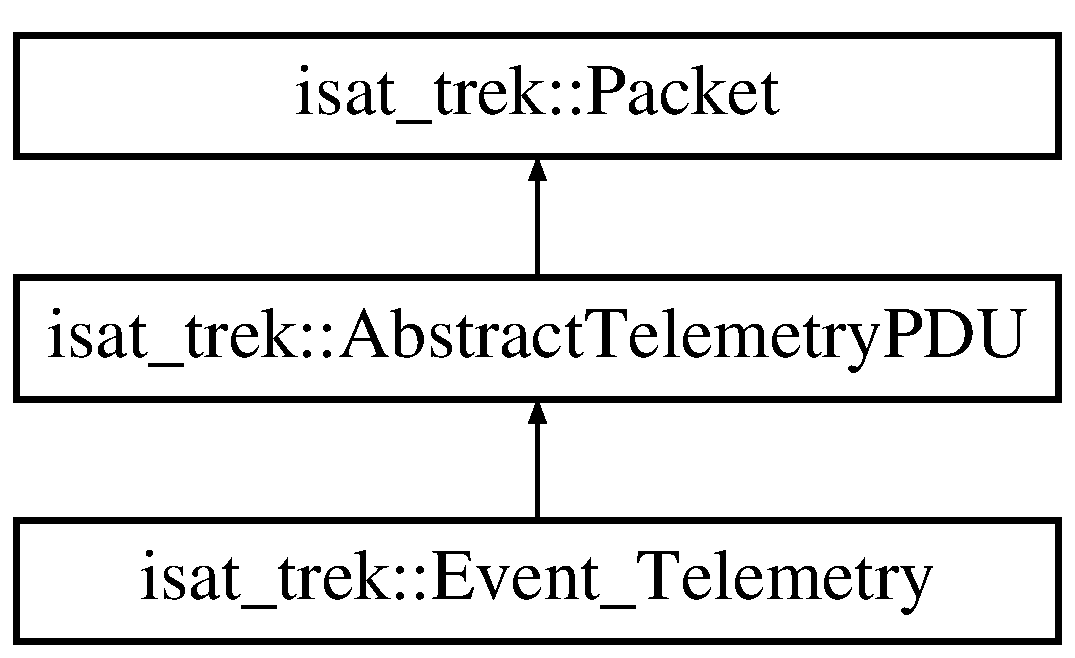
\includegraphics[height=3.000000cm]{classisat__trek_1_1_event___telemetry}
\end{center}
\end{figure}
\subsection*{Public Member Functions}
\begin{DoxyCompactItemize}
\item 
virtual bool \hyperlink{classisat__trek_1_1_event___telemetry_aeea8da6424ee67eec4783cf53fcce4ca}{from\+Bytes} (Byte\+Buffer \&buf)
\item 
virtual bool \hyperlink{classisat__trek_1_1_event___telemetry_aedaa07bcddc941db908689f3289213e5}{to\+Bytes} (Byte\+Buffer \&buf)
\end{DoxyCompactItemize}
\subsection*{Public Attributes}
\begin{DoxyCompactItemize}
\item 
int {\bfseries timestamp}\hypertarget{classisat__trek_1_1_event___telemetry_a1ddfd222fcc09dd7da710543cd368148}{}\label{classisat__trek_1_1_event___telemetry_a1ddfd222fcc09dd7da710543cd368148}

\item 
int {\bfseries type}\hypertarget{classisat__trek_1_1_event___telemetry_ac865ca7ad8d313ce40cf84e1036032a0}{}\label{classisat__trek_1_1_event___telemetry_ac865ca7ad8d313ce40cf84e1036032a0}

\item 
int {\bfseries severity}\hypertarget{classisat__trek_1_1_event___telemetry_a55ad53758f65fd0c32515a2ce903182c}{}\label{classisat__trek_1_1_event___telemetry_a55ad53758f65fd0c32515a2ce903182c}

\item 
int {\bfseries origin\+Id}\hypertarget{classisat__trek_1_1_event___telemetry_a233400eebddaeca29a85417b78445ad4}{}\label{classisat__trek_1_1_event___telemetry_a233400eebddaeca29a85417b78445ad4}

\item 
int {\bfseries code}\hypertarget{classisat__trek_1_1_event___telemetry_a6ff1f1fbee3c402ded8a60a4d8e799bd}{}\label{classisat__trek_1_1_event___telemetry_a6ff1f1fbee3c402ded8a60a4d8e799bd}

\item 
int {\bfseries message}\hypertarget{classisat__trek_1_1_event___telemetry_aebba74d8fcb7d175d36ae963ffca5c76}{}\label{classisat__trek_1_1_event___telemetry_aebba74d8fcb7d175d36ae963ffca5c76}

\end{DoxyCompactItemize}


\subsection{Member Function Documentation}
\index{isat\+\_\+trek\+::\+Event\+\_\+\+Telemetry@{isat\+\_\+trek\+::\+Event\+\_\+\+Telemetry}!from\+Bytes@{from\+Bytes}}
\index{from\+Bytes@{from\+Bytes}!isat\+\_\+trek\+::\+Event\+\_\+\+Telemetry@{isat\+\_\+trek\+::\+Event\+\_\+\+Telemetry}}
\subsubsection[{\texorpdfstring{from\+Bytes(\+Byte\+Buffer \&buf)}{fromBytes(ByteBuffer &buf)}}]{\setlength{\rightskip}{0pt plus 5cm}bool isat\+\_\+trek\+::\+Event\+\_\+\+Telemetry\+::from\+Bytes (
\begin{DoxyParamCaption}
\item[{Byte\+Buffer \&}]{buf}
\end{DoxyParamCaption}
)\hspace{0.3cm}{\ttfamily [virtual]}}\hypertarget{classisat__trek_1_1_event___telemetry_aeea8da6424ee67eec4783cf53fcce4ca}{}\label{classisat__trek_1_1_event___telemetry_aeea8da6424ee67eec4783cf53fcce4ca}
Populate the header and command fields from the data in buf.

\begin{DoxyReturn}{Returns}
true if successful. 
\end{DoxyReturn}


Implements \hyperlink{classisat__trek_1_1_packet}{isat\+\_\+trek\+::\+Packet}.

\index{isat\+\_\+trek\+::\+Event\+\_\+\+Telemetry@{isat\+\_\+trek\+::\+Event\+\_\+\+Telemetry}!to\+Bytes@{to\+Bytes}}
\index{to\+Bytes@{to\+Bytes}!isat\+\_\+trek\+::\+Event\+\_\+\+Telemetry@{isat\+\_\+trek\+::\+Event\+\_\+\+Telemetry}}
\subsubsection[{\texorpdfstring{to\+Bytes(\+Byte\+Buffer \&buf)}{toBytes(ByteBuffer &buf)}}]{\setlength{\rightskip}{0pt plus 5cm}bool isat\+\_\+trek\+::\+Event\+\_\+\+Telemetry\+::to\+Bytes (
\begin{DoxyParamCaption}
\item[{Byte\+Buffer \&}]{buf}
\end{DoxyParamCaption}
)\hspace{0.3cm}{\ttfamily [virtual]}}\hypertarget{classisat__trek_1_1_event___telemetry_aedaa07bcddc941db908689f3289213e5}{}\label{classisat__trek_1_1_event___telemetry_aedaa07bcddc941db908689f3289213e5}
Create the binary representation of this instance in the specified buffer.

\begin{DoxyReturn}{Returns}
true if successful. 
\end{DoxyReturn}


Implements \hyperlink{classisat__trek_1_1_packet}{isat\+\_\+trek\+::\+Packet}.



The documentation for this class was generated from the following files\+:\begin{DoxyCompactItemize}
\item 
/home/riley/work/fsw/src/isatgs/\+B\+A\+R\+Co\+Mm\+S/src/dependencies/trek/telemetry/Event\+\_\+\+Telemetry.\+h\item 
/home/riley/work/fsw/src/isatgs/\+B\+A\+R\+Co\+Mm\+S/src/dependencies/trek/telemetry/Event\+\_\+\+Telemetry.\+cpp\end{DoxyCompactItemize}

\hypertarget{classisat__utils_1_1_event_database}{}\section{isat\+\_\+utils\+:\+:Event\+Database Class Reference}
\label{classisat__utils_1_1_event_database}\index{isat\+\_\+utils\+::\+Event\+Database@{isat\+\_\+utils\+::\+Event\+Database}}
\subsection*{Classes}
\begin{DoxyCompactItemize}
\item 
struct \hyperlink{structisat__utils_1_1_event_database_1_1_event}{Event}
\item 
struct \hyperlink{structisat__utils_1_1_event_database_1_1_origin}{Origin}
\end{DoxyCompactItemize}
\subsection*{Public Member Functions}
\begin{DoxyCompactItemize}
\item 
{\bfseries Event\+Database} (std\+::string fn)\hypertarget{classisat__utils_1_1_event_database_a95e4339f0ada0594c15230daa2f390b6}{}\label{classisat__utils_1_1_event_database_a95e4339f0ada0594c15230daa2f390b6}

\item 
bool {\bfseries get\+Event} (int \hyperlink{struct_i_d}{ID}, \hyperlink{structisat__utils_1_1_event_database_1_1_event}{Event} \&event)\hypertarget{classisat__utils_1_1_event_database_ad8ec2a4837e06de362660317d13937d1}{}\label{classisat__utils_1_1_event_database_ad8ec2a4837e06de362660317d13937d1}

\item 
bool {\bfseries get\+Origin} (int \hyperlink{struct_i_d}{ID}, \hyperlink{structisat__utils_1_1_event_database_1_1_origin}{Origin} \&origin)\hypertarget{classisat__utils_1_1_event_database_ad279b48748c3b7edbfb273676e41ab83}{}\label{classisat__utils_1_1_event_database_ad279b48748c3b7edbfb273676e41ab83}

\item 
void {\bfseries load} (std\+::string)\hypertarget{classisat__utils_1_1_event_database_a9c0a42de9196cabca75f9196a0ebdf08}{}\label{classisat__utils_1_1_event_database_a9c0a42de9196cabca75f9196a0ebdf08}

\end{DoxyCompactItemize}
\subsection*{Public Attributes}
\begin{DoxyCompactItemize}
\item 
std\+::vector$<$ \hyperlink{structisat__utils_1_1_event_database_1_1_event}{Event} $>$ {\bfseries event\+DB}\hypertarget{classisat__utils_1_1_event_database_a4a8c02c3743ba490fc83f61b64761894}{}\label{classisat__utils_1_1_event_database_a4a8c02c3743ba490fc83f61b64761894}

\item 
std\+::vector$<$ \hyperlink{structisat__utils_1_1_event_database_1_1_origin}{Origin} $>$ {\bfseries origin\+DB}\hypertarget{classisat__utils_1_1_event_database_a8448b1621a77477f6bd7d720d277ecd9}{}\label{classisat__utils_1_1_event_database_a8448b1621a77477f6bd7d720d277ecd9}

\end{DoxyCompactItemize}


The documentation for this class was generated from the following files\+:\begin{DoxyCompactItemize}
\item 
/home/riley/work/fsw/src/isatgs/\+B\+A\+R\+Co\+Mm\+S/src/dependencies/utils/Event\+Database.\+h\item 
/home/riley/work/fsw/src/isatgs/\+B\+A\+R\+Co\+Mm\+S/src/dependencies/utils/Event\+Database.\+cpp\end{DoxyCompactItemize}

\hypertarget{struct_graph_1_1_event_item}{}\section{Graph\+:\+:Event\+Item Struct Reference}
\label{struct_graph_1_1_event_item}\index{Graph\+::\+Event\+Item@{Graph\+::\+Event\+Item}}
\subsection*{Public Types}
\begin{DoxyCompactItemize}
\item 
enum {\bfseries Rect\+Type} \{ {\bfseries Unstarted}, 
{\bfseries Paired}, 
{\bfseries Unfinished}
 \}\hypertarget{struct_graph_1_1_event_item_acf9786e04fdd442af0a2fb1c96bf4d88}{}\label{struct_graph_1_1_event_item_acf9786e04fdd442af0a2fb1c96bf4d88}

\end{DoxyCompactItemize}
\subsection*{Public Member Functions}
\begin{DoxyCompactItemize}
\item 
{\bfseries Event\+Item} (std\+::vector$<$ Q\+Graphics\+Ellipse\+Item $\ast$ $>$, \hyperlink{class_b_c___event}{B\+C\+\_\+\+Event} $\ast$)\hypertarget{struct_graph_1_1_event_item_aaad426402cf429da647b1ab05c8dfa73}{}\label{struct_graph_1_1_event_item_aaad426402cf429da647b1ab05c8dfa73}

\item 
{\bfseries Event\+Item} (std\+::vector$<$ Q\+Graphics\+Rect\+Item $\ast$ $>$, Rect\+Type, \hyperlink{class_b_c___event}{B\+C\+\_\+\+Event} $\ast$)\hypertarget{struct_graph_1_1_event_item_a3f8907f6ad3061fe654b908b55d7979c}{}\label{struct_graph_1_1_event_item_a3f8907f6ad3061fe654b908b55d7979c}

\item 
{\bfseries Event\+Item} (std\+::vector$<$ Q\+Graphics\+Rect\+Item $\ast$ $>$, Rect\+Type, \hyperlink{class_b_c___event}{B\+C\+\_\+\+Event}, \hyperlink{class_b_c___event}{B\+C\+\_\+\+Event} $\ast$)\hypertarget{struct_graph_1_1_event_item_ad027ec26db668cb89ca3a332589d27d1}{}\label{struct_graph_1_1_event_item_ad027ec26db668cb89ca3a332589d27d1}

\end{DoxyCompactItemize}
\subsection*{Public Attributes}
\begin{DoxyCompactItemize}
\item 
\hyperlink{class_b_c___event}{B\+C\+\_\+\+Event} $\ast$ {\bfseries event}\hypertarget{struct_graph_1_1_event_item_a1fe7fac5bfe82471c0f99b27685cdca2}{}\label{struct_graph_1_1_event_item_a1fe7fac5bfe82471c0f99b27685cdca2}

\item 
\hyperlink{class_b_c___event}{B\+C\+\_\+\+Event} {\bfseries pevents}\hypertarget{struct_graph_1_1_event_item_ae23ec75f6d3edd58d5ff121f463abbb3}{}\label{struct_graph_1_1_event_item_ae23ec75f6d3edd58d5ff121f463abbb3}

\item 
\hyperlink{class_b_c___event}{B\+C\+\_\+\+Event} $\ast$ {\bfseries peventf}\hypertarget{struct_graph_1_1_event_item_ad553ac00e7fb52be7c183a92c64c26bc}{}\label{struct_graph_1_1_event_item_ad553ac00e7fb52be7c183a92c64c26bc}

\item 
\hyperlink{class_b_c___d_i_t_l___s_e_v_t_r_e_e___i_t_e_m}{B\+C\+\_\+\+D\+I\+T\+L\+\_\+\+S\+E\+V\+T\+R\+E\+E\+\_\+\+I\+T\+EM} $\ast$ {\bfseries tree\+Item}\hypertarget{struct_graph_1_1_event_item_a8fd8ea204630af864ef6465b230f0806}{}\label{struct_graph_1_1_event_item_a8fd8ea204630af864ef6465b230f0806}

\item 
Q\+Graphics\+Pixmap\+Item $\ast$ {\bfseries unbounded\+Event\+Arrow}\hypertarget{struct_graph_1_1_event_item_afbde0eb07aef4413e1ec45f1b2d2946a}{}\label{struct_graph_1_1_event_item_afbde0eb07aef4413e1ec45f1b2d2946a}

\item 
std\+::vector$<$ Q\+Graphics\+Item $\ast$ $>$ {\bfseries graphics\+Items}\hypertarget{struct_graph_1_1_event_item_a3c44521bc6bed06d14c03239e357a63b}{}\label{struct_graph_1_1_event_item_a3c44521bc6bed06d14c03239e357a63b}

\item 
Rect\+Type {\bfseries type}\hypertarget{struct_graph_1_1_event_item_a3bd60dae1aa172849bb2e293fc05bbde}{}\label{struct_graph_1_1_event_item_a3bd60dae1aa172849bb2e293fc05bbde}

\end{DoxyCompactItemize}


The documentation for this struct was generated from the following files\+:\begin{DoxyCompactItemize}
\item 
/home/riley/work/fsw/src/isatgs/\+B\+A\+R\+Co\+Mm\+S/src/modules/\+B\+A\+R\+Co\+Mm\+S\+\_\+\+D\+I\+T\+L/bc\+\_\+ditl\+\_\+graph.\+h\item 
/home/riley/work/fsw/src/isatgs/\+B\+A\+R\+Co\+Mm\+S/src/modules/\+B\+A\+R\+Co\+Mm\+S\+\_\+\+D\+I\+T\+L/bc\+\_\+ditl\+\_\+graph.\+cpp\end{DoxyCompactItemize}

\hypertarget{classisat__utils_1_1_event_logger}{}\section{isat\+\_\+utils\+:\+:Event\+Logger Class Reference}
\label{classisat__utils_1_1_event_logger}\index{isat\+\_\+utils\+::\+Event\+Logger@{isat\+\_\+utils\+::\+Event\+Logger}}


{\ttfamily \#include $<$Event\+Logger.\+h$>$}

\subsection*{Public Member Functions}
\begin{DoxyCompactItemize}
\item 
\hyperlink{classisat__utils_1_1_event_logger_aa388db265b9d3ae2267bdb92a3a348fa}{Event\+Logger} (int origin, std\+::string file)
\item 
void \hyperlink{classisat__utils_1_1_event_logger_afa7b30b55dde728d55e5fb1cd865d768}{advisory} (int event\+Code, int linenum, std\+::string message=\char`\"{}\char`\"{})
\item 
void \hyperlink{classisat__utils_1_1_event_logger_abc20515e43ecdcdaa8cdcf85c1e0aa87}{advisory\+Start} (int event\+Code, int linenum, std\+::string message=\char`\"{}\char`\"{})
\item 
void {\bfseries advisory\+End} (int event\+Code, int linenum, std\+::string message=\char`\"{}\char`\"{})\hypertarget{classisat__utils_1_1_event_logger_a40144ea68f8f43f09dd3d9ed3079be44}{}\label{classisat__utils_1_1_event_logger_a40144ea68f8f43f09dd3d9ed3079be44}

\end{DoxyCompactItemize}
\subsection*{Protected Attributes}
\begin{DoxyCompactItemize}
\item 
int {\bfseries origin}\hypertarget{classisat__utils_1_1_event_logger_a8395abd5c58cfcc3272d277bbdb1d453}{}\label{classisat__utils_1_1_event_logger_a8395abd5c58cfcc3272d277bbdb1d453}

\item 
std\+::string {\bfseries file}\hypertarget{classisat__utils_1_1_event_logger_aa7129e5a84e978151f2432d7a43dcdb9}{}\label{classisat__utils_1_1_event_logger_aa7129e5a84e978151f2432d7a43dcdb9}

\end{DoxyCompactItemize}


\subsection{Detailed Description}
Adaptor for Even\+Manager. Makes it easy(er) to create and log events. 

\subsection{Constructor \& Destructor Documentation}
\index{isat\+\_\+utils\+::\+Event\+Logger@{isat\+\_\+utils\+::\+Event\+Logger}!Event\+Logger@{Event\+Logger}}
\index{Event\+Logger@{Event\+Logger}!isat\+\_\+utils\+::\+Event\+Logger@{isat\+\_\+utils\+::\+Event\+Logger}}
\subsubsection[{\texorpdfstring{Event\+Logger(int origin, std\+::string file)}{EventLogger(int origin, std::string file)}}]{\setlength{\rightskip}{0pt plus 5cm}isat\+\_\+utils\+::\+Event\+Logger\+::\+Event\+Logger (
\begin{DoxyParamCaption}
\item[{int}]{origin, }
\item[{std\+::string}]{file}
\end{DoxyParamCaption}
)}\hypertarget{classisat__utils_1_1_event_logger_aa388db265b9d3ae2267bdb92a3a348fa}{}\label{classisat__utils_1_1_event_logger_aa388db265b9d3ae2267bdb92a3a348fa}
Create an \hyperlink{classisat__utils_1_1_event_logger}{Event\+Logger} that will log events with the specified origin and file. 

\subsection{Member Function Documentation}
\index{isat\+\_\+utils\+::\+Event\+Logger@{isat\+\_\+utils\+::\+Event\+Logger}!advisory@{advisory}}
\index{advisory@{advisory}!isat\+\_\+utils\+::\+Event\+Logger@{isat\+\_\+utils\+::\+Event\+Logger}}
\subsubsection[{\texorpdfstring{advisory(int event\+Code, int linenum, std\+::string message="""")}{advisory(int eventCode, int linenum, std::string message="")}}]{\setlength{\rightskip}{0pt plus 5cm}void isat\+\_\+utils\+::\+Event\+Logger\+::advisory (
\begin{DoxyParamCaption}
\item[{int}]{event\+Code, }
\item[{int}]{linenum, }
\item[{std\+::string}]{message = {\ttfamily \char`\"{}\char`\"{}}}
\end{DoxyParamCaption}
)}\hypertarget{classisat__utils_1_1_event_logger_afa7b30b55dde728d55e5fb1cd865d768}{}\label{classisat__utils_1_1_event_logger_afa7b30b55dde728d55e5fb1cd865d768}
Issue an advisory level point event (single instant in time). \index{isat\+\_\+utils\+::\+Event\+Logger@{isat\+\_\+utils\+::\+Event\+Logger}!advisory\+Start@{advisory\+Start}}
\index{advisory\+Start@{advisory\+Start}!isat\+\_\+utils\+::\+Event\+Logger@{isat\+\_\+utils\+::\+Event\+Logger}}
\subsubsection[{\texorpdfstring{advisory\+Start(int event\+Code, int linenum, std\+::string message="""")}{advisoryStart(int eventCode, int linenum, std::string message="")}}]{\setlength{\rightskip}{0pt plus 5cm}void isat\+\_\+utils\+::\+Event\+Logger\+::advisory\+Start (
\begin{DoxyParamCaption}
\item[{int}]{event\+Code, }
\item[{int}]{linenum, }
\item[{std\+::string}]{message = {\ttfamily \char`\"{}\char`\"{}}}
\end{DoxyParamCaption}
)}\hypertarget{classisat__utils_1_1_event_logger_abc20515e43ecdcdaa8cdcf85c1e0aa87}{}\label{classisat__utils_1_1_event_logger_abc20515e43ecdcdaa8cdcf85c1e0aa87}
Issue and advisory level range event. This is the start of the range. 

The documentation for this class was generated from the following file\+:\begin{DoxyCompactItemize}
\item 
/home/riley/work/fsw/src/isatgs/\+B\+A\+R\+Co\+Mm\+S/src/dependencies/utils/Event\+Logger.\+h\end{DoxyCompactItemize}

\hypertarget{classisat__utils_1_1_event_manager}{}\section{isat\+\_\+utils\+:\+:Event\+Manager Class Reference}
\label{classisat__utils_1_1_event_manager}\index{isat\+\_\+utils\+::\+Event\+Manager@{isat\+\_\+utils\+::\+Event\+Manager}}
\subsection*{Public Member Functions}
\begin{DoxyCompactItemize}
\item 
void \hyperlink{classisat__utils_1_1_event_manager_a8ae01f4eeb365b1ead6e81d38ae78195}{log\+Event} (\hyperlink{classisat__utils_1_1_event}{Event} event)
\item 
bool \hyperlink{classisat__utils_1_1_event_manager_ab95b464d5fdde2902c144c0445fbda75}{has\+Events} () const 
\item 
bool \hyperlink{classisat__utils_1_1_event_manager_acfb496b37edf922713c7a372dfacd80e}{get\+Event} (\hyperlink{classisat__utils_1_1_event}{Event} \&event)
\end{DoxyCompactItemize}
\subsection*{Static Public Member Functions}
\begin{DoxyCompactItemize}
\item 
static \hyperlink{classisat__utils_1_1_event_manager}{Event\+Manager} \& {\bfseries get\+Instance} ()\hypertarget{classisat__utils_1_1_event_manager_ab4cb6141ba60fb9fb4fbdfdb083c4a1b}{}\label{classisat__utils_1_1_event_manager_ab4cb6141ba60fb9fb4fbdfdb083c4a1b}

\end{DoxyCompactItemize}
\subsection*{Protected Attributes}
\begin{DoxyCompactItemize}
\item 
std\+::deque$<$ \hyperlink{classisat__utils_1_1_event}{Event} $>$ {\bfseries event\+Queue}\hypertarget{classisat__utils_1_1_event_manager_ab32d83c25318106a3dd2c2e4488f1789}{}\label{classisat__utils_1_1_event_manager_ab32d83c25318106a3dd2c2e4488f1789}

\item 
boost\+::mutex {\bfseries queue\+Mutex}\hypertarget{classisat__utils_1_1_event_manager_a36a612e1e1af43922b18d9efacad5853}{}\label{classisat__utils_1_1_event_manager_a36a612e1e1af43922b18d9efacad5853}

\end{DoxyCompactItemize}


\subsection{Member Function Documentation}
\index{isat\+\_\+utils\+::\+Event\+Manager@{isat\+\_\+utils\+::\+Event\+Manager}!get\+Event@{get\+Event}}
\index{get\+Event@{get\+Event}!isat\+\_\+utils\+::\+Event\+Manager@{isat\+\_\+utils\+::\+Event\+Manager}}
\subsubsection[{\texorpdfstring{get\+Event(\+Event \&event)}{getEvent(Event &event)}}]{\setlength{\rightskip}{0pt plus 5cm}bool isat\+\_\+utils\+::\+Event\+Manager\+::get\+Event (
\begin{DoxyParamCaption}
\item[{{\bf Event} \&}]{event}
\end{DoxyParamCaption}
)}\hypertarget{classisat__utils_1_1_event_manager_acfb496b37edf922713c7a372dfacd80e}{}\label{classisat__utils_1_1_event_manager_acfb496b37edf922713c7a372dfacd80e}
Gets the next event in the queue, returns true. Returns false if there are no events. \index{isat\+\_\+utils\+::\+Event\+Manager@{isat\+\_\+utils\+::\+Event\+Manager}!has\+Events@{has\+Events}}
\index{has\+Events@{has\+Events}!isat\+\_\+utils\+::\+Event\+Manager@{isat\+\_\+utils\+::\+Event\+Manager}}
\subsubsection[{\texorpdfstring{has\+Events() const }{hasEvents() const }}]{\setlength{\rightskip}{0pt plus 5cm}bool isat\+\_\+utils\+::\+Event\+Manager\+::has\+Events (
\begin{DoxyParamCaption}
{}
\end{DoxyParamCaption}
) const}\hypertarget{classisat__utils_1_1_event_manager_ab95b464d5fdde2902c144c0445fbda75}{}\label{classisat__utils_1_1_event_manager_ab95b464d5fdde2902c144c0445fbda75}
Returns true if there are events in the event queue. \index{isat\+\_\+utils\+::\+Event\+Manager@{isat\+\_\+utils\+::\+Event\+Manager}!log\+Event@{log\+Event}}
\index{log\+Event@{log\+Event}!isat\+\_\+utils\+::\+Event\+Manager@{isat\+\_\+utils\+::\+Event\+Manager}}
\subsubsection[{\texorpdfstring{log\+Event(\+Event event)}{logEvent(Event event)}}]{\setlength{\rightskip}{0pt plus 5cm}void isat\+\_\+utils\+::\+Event\+Manager\+::log\+Event (
\begin{DoxyParamCaption}
\item[{{\bf Event}}]{event}
\end{DoxyParamCaption}
)}\hypertarget{classisat__utils_1_1_event_manager_a8ae01f4eeb365b1ead6e81d38ae78195}{}\label{classisat__utils_1_1_event_manager_a8ae01f4eeb365b1ead6e81d38ae78195}
Issue a point event (single instant in time). 

The documentation for this class was generated from the following files\+:\begin{DoxyCompactItemize}
\item 
/home/riley/work/fsw/src/isatgs/\+B\+A\+R\+Co\+Mm\+S/src/dependencies/utils/Event\+Manager.\+h\item 
/home/riley/work/fsw/src/isatgs/\+B\+A\+R\+Co\+Mm\+S/src/dependencies/utils/Event\+Manager.\+cpp\end{DoxyCompactItemize}

\hypertarget{classisat__trek_1_1_event_retrans___command}{}\section{isat\+\_\+trek\+:\+:Event\+Retrans\+\_\+\+Command Class Reference}
\label{classisat__trek_1_1_event_retrans___command}\index{isat\+\_\+trek\+::\+Event\+Retrans\+\_\+\+Command@{isat\+\_\+trek\+::\+Event\+Retrans\+\_\+\+Command}}


{\ttfamily \#include $<$Event\+Retrans\+\_\+\+Command.\+h$>$}

Inheritance diagram for isat\+\_\+trek\+:\+:Event\+Retrans\+\_\+\+Command\+:\begin{figure}[H]
\begin{center}
\leavevmode
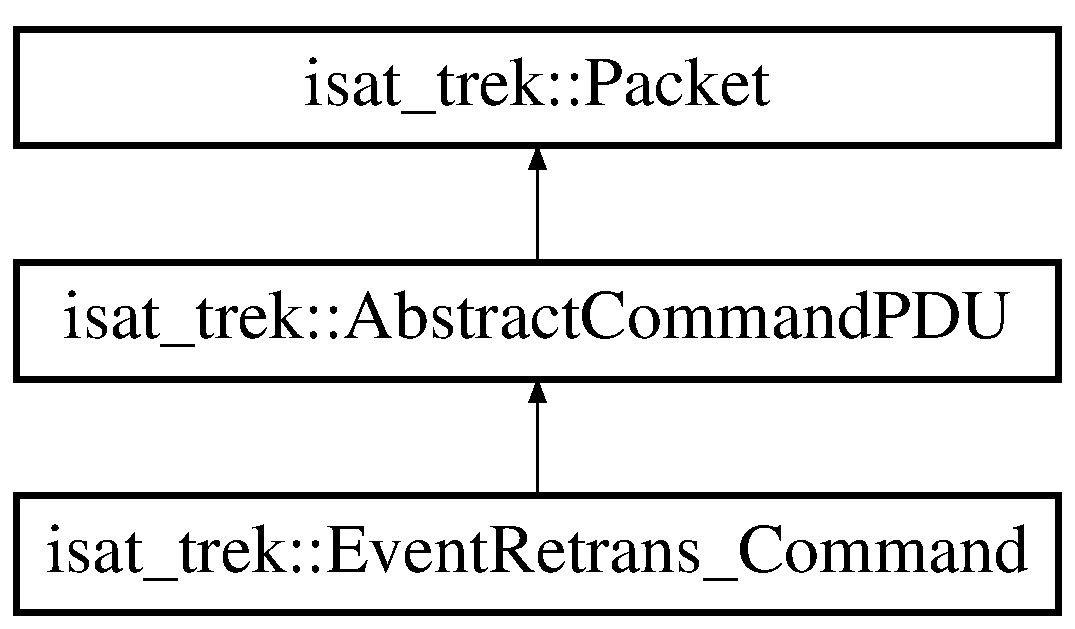
\includegraphics[height=3.000000cm]{classisat__trek_1_1_event_retrans___command}
\end{center}
\end{figure}
\subsection*{Public Member Functions}
\begin{DoxyCompactItemize}
\item 
bool \hyperlink{classisat__trek_1_1_event_retrans___command_a54fbca0dd27fbb2a44718b160caeb266}{from\+Bytes} (Byte\+Buffer \&buf)
\item 
bool \hyperlink{classisat__trek_1_1_event_retrans___command_ae989b246384d73d1c4cac682672676a3}{to\+Bytes} (Byte\+Buffer \&buf)
\end{DoxyCompactItemize}
\subsection*{Public Attributes}
\begin{DoxyCompactItemize}
\item 
int {\bfseries object\+Id} = 0\hypertarget{classisat__trek_1_1_event_retrans___command_a6b6df7f1ca81ef01d8ef8db6dd1a8ff3}{}\label{classisat__trek_1_1_event_retrans___command_a6b6df7f1ca81ef01d8ef8db6dd1a8ff3}

\end{DoxyCompactItemize}


\subsection{Detailed Description}
X\+XX\+: Replace with real description in isat.\+pdu file. 

\subsection{Member Function Documentation}
\index{isat\+\_\+trek\+::\+Event\+Retrans\+\_\+\+Command@{isat\+\_\+trek\+::\+Event\+Retrans\+\_\+\+Command}!from\+Bytes@{from\+Bytes}}
\index{from\+Bytes@{from\+Bytes}!isat\+\_\+trek\+::\+Event\+Retrans\+\_\+\+Command@{isat\+\_\+trek\+::\+Event\+Retrans\+\_\+\+Command}}
\subsubsection[{\texorpdfstring{from\+Bytes(\+Byte\+Buffer \&buf)}{fromBytes(ByteBuffer &buf)}}]{\setlength{\rightskip}{0pt plus 5cm}bool isat\+\_\+trek\+::\+Event\+Retrans\+\_\+\+Command\+::from\+Bytes (
\begin{DoxyParamCaption}
\item[{Byte\+Buffer \&}]{buf}
\end{DoxyParamCaption}
)\hspace{0.3cm}{\ttfamily [virtual]}}\hypertarget{classisat__trek_1_1_event_retrans___command_a54fbca0dd27fbb2a44718b160caeb266}{}\label{classisat__trek_1_1_event_retrans___command_a54fbca0dd27fbb2a44718b160caeb266}
Populate the header and command fields from the data in buf.

\begin{DoxyReturn}{Returns}
true if successful. 
\end{DoxyReturn}


Implements \hyperlink{classisat__trek_1_1_packet}{isat\+\_\+trek\+::\+Packet}.

\index{isat\+\_\+trek\+::\+Event\+Retrans\+\_\+\+Command@{isat\+\_\+trek\+::\+Event\+Retrans\+\_\+\+Command}!to\+Bytes@{to\+Bytes}}
\index{to\+Bytes@{to\+Bytes}!isat\+\_\+trek\+::\+Event\+Retrans\+\_\+\+Command@{isat\+\_\+trek\+::\+Event\+Retrans\+\_\+\+Command}}
\subsubsection[{\texorpdfstring{to\+Bytes(\+Byte\+Buffer \&buf)}{toBytes(ByteBuffer &buf)}}]{\setlength{\rightskip}{0pt plus 5cm}bool isat\+\_\+trek\+::\+Event\+Retrans\+\_\+\+Command\+::to\+Bytes (
\begin{DoxyParamCaption}
\item[{Byte\+Buffer \&}]{buf}
\end{DoxyParamCaption}
)\hspace{0.3cm}{\ttfamily [virtual]}}\hypertarget{classisat__trek_1_1_event_retrans___command_ae989b246384d73d1c4cac682672676a3}{}\label{classisat__trek_1_1_event_retrans___command_ae989b246384d73d1c4cac682672676a3}
Create the binary representation of this instance in the specified buffer.

\begin{DoxyReturn}{Returns}
true if successful. 
\end{DoxyReturn}


Implements \hyperlink{classisat__trek_1_1_packet}{isat\+\_\+trek\+::\+Packet}.



The documentation for this class was generated from the following files\+:\begin{DoxyCompactItemize}
\item 
/home/riley/work/fsw/src/isatgs/\+B\+A\+R\+Co\+Mm\+S/src/dependencies/trek/command/Event\+Retrans\+\_\+\+Command.\+h\item 
/home/riley/work/fsw/src/isatgs/\+B\+A\+R\+Co\+Mm\+S/src/dependencies/trek/command/Event\+Retrans\+\_\+\+Command.\+cpp\end{DoxyCompactItemize}

\hypertarget{struct_f_d}{}\section{FD Struct Reference}
\label{struct_f_d}\index{FD@{FD}}
\subsection*{Public Attributes}
\begin{DoxyCompactItemize}
\item 
u\+\_\+int\+\_\+4 {\bfseries offset}\hypertarget{struct_f_d_aa7a398c7effa71d334cd242533f19e51}{}\label{struct_f_d_aa7a398c7effa71d334cd242533f19e51}

\item 
u\+\_\+int\+\_\+1 {\bfseries buffer} \mbox{[}M\+A\+X\+\_\+\+F\+I\+L\+E\+\_\+\+C\+H\+U\+N\+K\+\_\+\+S\+I\+ZE+4\mbox{]}\hypertarget{struct_f_d_a3df38bc90ee8c4d6390784d6afa508c5}{}\label{struct_f_d_a3df38bc90ee8c4d6390784d6afa508c5}

\item 
u\+\_\+int\+\_\+2 {\bfseries buffer\+\_\+length}\hypertarget{struct_f_d_a9389d66689b2b1ba0f38e3c023b5eb42}{}\label{struct_f_d_a9389d66689b2b1ba0f38e3c023b5eb42}

\end{DoxyCompactItemize}


The documentation for this struct was generated from the following file\+:\begin{DoxyCompactItemize}
\item 
/home/riley/work/fsw/src/isatgs/\+B\+A\+R\+Co\+Mm\+S/src/dependencies/\+C\+F\+D\+P/\+P\+R\+I/structures.\+h\end{DoxyCompactItemize}

\hypertarget{classisat__utils_1_1_file}{}\section{isat\+\_\+utils\+:\+:File Class Reference}
\label{classisat__utils_1_1_file}\index{isat\+\_\+utils\+::\+File@{isat\+\_\+utils\+::\+File}}


{\ttfamily \#include $<$File.\+h$>$}

\subsection*{Public Member Functions}
\begin{DoxyCompactItemize}
\item 
\hyperlink{classisat__utils_1_1_file_ab5c27e041ed561bc2f4df177729e3a16}{File} (\hyperlink{classisat__utils_1_1_string}{String} name)
\item 
{\bfseries File} (\hyperlink{classisat__utils_1_1_file}{File} const \&rhs)\hypertarget{classisat__utils_1_1_file_af7d0caa9d270dec2ba47b7480f830f6a}{}\label{classisat__utils_1_1_file_af7d0caa9d270dec2ba47b7480f830f6a}

\item 
\hyperlink{classisat__utils_1_1_file}{File} \& {\bfseries operator=} (\hyperlink{classisat__utils_1_1_file}{File} rhs)\hypertarget{classisat__utils_1_1_file_a0707325fdb0f0d7e30b4dded4ca12968}{}\label{classisat__utils_1_1_file_a0707325fdb0f0d7e30b4dded4ca12968}

\item 
\hyperlink{classisat__utils_1_1_string}{String} \hyperlink{classisat__utils_1_1_file_a622367fe6c4acc18c1bc17d4622828da}{get\+Name} () const 
\item 
bool \hyperlink{classisat__utils_1_1_file_a4aac599cc77dd555da5139af109a0a8c}{exists} () const 
\item 
bool \hyperlink{classisat__utils_1_1_file_a4094a6e3a043afb50aa01244788c2d3e}{is\+File} () const 
\item 
bool \hyperlink{classisat__utils_1_1_file_ab701f989381170817b3d6d5f1538aa04}{is\+Directory} () const 
\item 
long \hyperlink{classisat__utils_1_1_file_a0a727f4f870d89361fbe5de225669edc}{length} () const 
\item 
long \hyperlink{classisat__utils_1_1_file_a4fb268c3238647d98fc09055341d3350}{last\+Access\+Time} () const 
\item 
long \hyperlink{classisat__utils_1_1_file_a70413578e0552a9d6b68f11c76a257f4}{last\+Data\+Modification\+Time} () const 
\item 
long \hyperlink{classisat__utils_1_1_file_ab6161b7629ab9316452e0a6c012fe5ed}{last\+Status\+Change\+Time} () const 
\item 
\hyperlink{classisat__utils_1_1_array_list}{Array\+List}$<$ \hyperlink{classisat__utils_1_1_string}{String} $>$ \hyperlink{classisat__utils_1_1_file_afa2650abc47107da9d3ec39d74c50043}{list} () const 
\end{DoxyCompactItemize}


\subsection{Detailed Description}
Operations on a file or directory.

Inspired by Java\textquotesingle{}s \hyperlink{classisat__utils_1_1_file}{File} class, this class provides common operations on files and directories. Any additional operations added should be named the same (and as much as possible, act the same) as the Java \hyperlink{classisat__utils_1_1_file}{File} class. 

\subsection{Constructor \& Destructor Documentation}
\index{isat\+\_\+utils\+::\+File@{isat\+\_\+utils\+::\+File}!File@{File}}
\index{File@{File}!isat\+\_\+utils\+::\+File@{isat\+\_\+utils\+::\+File}}
\subsubsection[{\texorpdfstring{File(\+String name)}{File(String name)}}]{\setlength{\rightskip}{0pt plus 5cm}isat\+\_\+utils\+::\+File\+::\+File (
\begin{DoxyParamCaption}
\item[{{\bf String}}]{name}
\end{DoxyParamCaption}
)}\hypertarget{classisat__utils_1_1_file_ab5c27e041ed561bc2f4df177729e3a16}{}\label{classisat__utils_1_1_file_ab5c27e041ed561bc2f4df177729e3a16}
Creates a \hyperlink{classisat__utils_1_1_file}{File} instance from the given path name. 

\subsection{Member Function Documentation}
\index{isat\+\_\+utils\+::\+File@{isat\+\_\+utils\+::\+File}!exists@{exists}}
\index{exists@{exists}!isat\+\_\+utils\+::\+File@{isat\+\_\+utils\+::\+File}}
\subsubsection[{\texorpdfstring{exists() const }{exists() const }}]{\setlength{\rightskip}{0pt plus 5cm}bool isat\+\_\+utils\+::\+File\+::exists (
\begin{DoxyParamCaption}
{}
\end{DoxyParamCaption}
) const}\hypertarget{classisat__utils_1_1_file_a4aac599cc77dd555da5139af109a0a8c}{}\label{classisat__utils_1_1_file_a4aac599cc77dd555da5139af109a0a8c}
Determine if the file or directory represented by path name exists.

\begin{DoxyReturn}{Returns}
true if the pathname exists. 
\end{DoxyReturn}
\index{isat\+\_\+utils\+::\+File@{isat\+\_\+utils\+::\+File}!get\+Name@{get\+Name}}
\index{get\+Name@{get\+Name}!isat\+\_\+utils\+::\+File@{isat\+\_\+utils\+::\+File}}
\subsubsection[{\texorpdfstring{get\+Name() const }{getName() const }}]{\setlength{\rightskip}{0pt plus 5cm}{\bf String} isat\+\_\+utils\+::\+File\+::get\+Name (
\begin{DoxyParamCaption}
{}
\end{DoxyParamCaption}
) const}\hypertarget{classisat__utils_1_1_file_a622367fe6c4acc18c1bc17d4622828da}{}\label{classisat__utils_1_1_file_a622367fe6c4acc18c1bc17d4622828da}
Returns the path name represented by this instance.

\begin{DoxyReturn}{Returns}
the path name of the instance. 
\end{DoxyReturn}
\index{isat\+\_\+utils\+::\+File@{isat\+\_\+utils\+::\+File}!is\+Directory@{is\+Directory}}
\index{is\+Directory@{is\+Directory}!isat\+\_\+utils\+::\+File@{isat\+\_\+utils\+::\+File}}
\subsubsection[{\texorpdfstring{is\+Directory() const }{isDirectory() const }}]{\setlength{\rightskip}{0pt plus 5cm}bool isat\+\_\+utils\+::\+File\+::is\+Directory (
\begin{DoxyParamCaption}
{}
\end{DoxyParamCaption}
) const}\hypertarget{classisat__utils_1_1_file_ab701f989381170817b3d6d5f1538aa04}{}\label{classisat__utils_1_1_file_ab701f989381170817b3d6d5f1538aa04}
Determine if the path name in this instance is a directory.

\begin{DoxyReturn}{Returns}
true if the path name is a directory. 
\end{DoxyReturn}
\index{isat\+\_\+utils\+::\+File@{isat\+\_\+utils\+::\+File}!is\+File@{is\+File}}
\index{is\+File@{is\+File}!isat\+\_\+utils\+::\+File@{isat\+\_\+utils\+::\+File}}
\subsubsection[{\texorpdfstring{is\+File() const }{isFile() const }}]{\setlength{\rightskip}{0pt plus 5cm}bool isat\+\_\+utils\+::\+File\+::is\+File (
\begin{DoxyParamCaption}
{}
\end{DoxyParamCaption}
) const}\hypertarget{classisat__utils_1_1_file_a4094a6e3a043afb50aa01244788c2d3e}{}\label{classisat__utils_1_1_file_a4094a6e3a043afb50aa01244788c2d3e}
Determine if the path name in this instance is a file.

\begin{DoxyReturn}{Returns}
true if the path name is a file. 
\end{DoxyReturn}
\index{isat\+\_\+utils\+::\+File@{isat\+\_\+utils\+::\+File}!last\+Access\+Time@{last\+Access\+Time}}
\index{last\+Access\+Time@{last\+Access\+Time}!isat\+\_\+utils\+::\+File@{isat\+\_\+utils\+::\+File}}
\subsubsection[{\texorpdfstring{last\+Access\+Time() const }{lastAccessTime() const }}]{\setlength{\rightskip}{0pt plus 5cm}long isat\+\_\+utils\+::\+File\+::last\+Access\+Time (
\begin{DoxyParamCaption}
{}
\end{DoxyParamCaption}
) const}\hypertarget{classisat__utils_1_1_file_a4fb268c3238647d98fc09055341d3350}{}\label{classisat__utils_1_1_file_a4fb268c3238647d98fc09055341d3350}
Get the atime for this instance.

\begin{DoxyReturn}{Returns}
The last access time in seconds from the unix epoch. 
\end{DoxyReturn}
\index{isat\+\_\+utils\+::\+File@{isat\+\_\+utils\+::\+File}!last\+Data\+Modification\+Time@{last\+Data\+Modification\+Time}}
\index{last\+Data\+Modification\+Time@{last\+Data\+Modification\+Time}!isat\+\_\+utils\+::\+File@{isat\+\_\+utils\+::\+File}}
\subsubsection[{\texorpdfstring{last\+Data\+Modification\+Time() const }{lastDataModificationTime() const }}]{\setlength{\rightskip}{0pt plus 5cm}long isat\+\_\+utils\+::\+File\+::last\+Data\+Modification\+Time (
\begin{DoxyParamCaption}
{}
\end{DoxyParamCaption}
) const}\hypertarget{classisat__utils_1_1_file_a70413578e0552a9d6b68f11c76a257f4}{}\label{classisat__utils_1_1_file_a70413578e0552a9d6b68f11c76a257f4}
Get the mtime for this instance.

\begin{DoxyReturn}{Returns}
The last data modification time in seconds from the unix epoch. 
\end{DoxyReturn}
\index{isat\+\_\+utils\+::\+File@{isat\+\_\+utils\+::\+File}!last\+Status\+Change\+Time@{last\+Status\+Change\+Time}}
\index{last\+Status\+Change\+Time@{last\+Status\+Change\+Time}!isat\+\_\+utils\+::\+File@{isat\+\_\+utils\+::\+File}}
\subsubsection[{\texorpdfstring{last\+Status\+Change\+Time() const }{lastStatusChangeTime() const }}]{\setlength{\rightskip}{0pt plus 5cm}long isat\+\_\+utils\+::\+File\+::last\+Status\+Change\+Time (
\begin{DoxyParamCaption}
{}
\end{DoxyParamCaption}
) const}\hypertarget{classisat__utils_1_1_file_ab6161b7629ab9316452e0a6c012fe5ed}{}\label{classisat__utils_1_1_file_ab6161b7629ab9316452e0a6c012fe5ed}
Get the ctime for this instance.

\begin{DoxyReturn}{Returns}
The last status change time in seconds from the unix epoch. 
\end{DoxyReturn}
\index{isat\+\_\+utils\+::\+File@{isat\+\_\+utils\+::\+File}!length@{length}}
\index{length@{length}!isat\+\_\+utils\+::\+File@{isat\+\_\+utils\+::\+File}}
\subsubsection[{\texorpdfstring{length() const }{length() const }}]{\setlength{\rightskip}{0pt plus 5cm}long isat\+\_\+utils\+::\+File\+::length (
\begin{DoxyParamCaption}
{}
\end{DoxyParamCaption}
) const}\hypertarget{classisat__utils_1_1_file_a0a727f4f870d89361fbe5de225669edc}{}\label{classisat__utils_1_1_file_a0a727f4f870d89361fbe5de225669edc}
Determine the length of the file specified by this instance\textquotesingle{}s path name.

\begin{DoxyReturn}{Returns}
The length of the file in bytes. Returns 0 if the file is unreadable or if it\textquotesingle{}s not a file. This is not what you\textquotesingle{}d want, but we can\textquotesingle{}t throw an exception for an error, so make sure the file exists and is a file before you ask for the length. \+:) 
\end{DoxyReturn}
\index{isat\+\_\+utils\+::\+File@{isat\+\_\+utils\+::\+File}!list@{list}}
\index{list@{list}!isat\+\_\+utils\+::\+File@{isat\+\_\+utils\+::\+File}}
\subsubsection[{\texorpdfstring{list() const }{list() const }}]{\setlength{\rightskip}{0pt plus 5cm}{\bf Array\+List}$<$ {\bf String} $>$ isat\+\_\+utils\+::\+File\+::list (
\begin{DoxyParamCaption}
{}
\end{DoxyParamCaption}
) const}\hypertarget{classisat__utils_1_1_file_afa2650abc47107da9d3ec39d74c50043}{}\label{classisat__utils_1_1_file_afa2650abc47107da9d3ec39d74c50043}
If this instance is a directory, return a list of files and directories contained within it.

\begin{DoxyReturn}{Returns}
a list of files and directories, or a zero length list if this instance is not a directory. 
\end{DoxyReturn}


The documentation for this class was generated from the following files\+:\begin{DoxyCompactItemize}
\item 
/home/riley/work/fsw/src/isatgs/\+B\+A\+R\+Co\+Mm\+S/src/dependencies/utils/File.\+h\item 
/home/riley/work/fsw/src/isatgs/\+B\+A\+R\+Co\+Mm\+S/src/dependencies/utils/File.\+cpp\end{DoxyCompactItemize}

\hypertarget{struct_f_i_n}{}\section{F\+IN Struct Reference}
\label{struct_f_i_n}\index{F\+IN@{F\+IN}}
\subsection*{Public Attributes}
\begin{DoxyCompactItemize}
\item 
u\+\_\+int\+\_\+1 {\bfseries condition\+\_\+code}\+: 4\hypertarget{struct_f_i_n_a016fb1f5c98239c8050e064e8523ed24}{}\label{struct_f_i_n_a016fb1f5c98239c8050e064e8523ed24}

\item 
u\+\_\+int\+\_\+1 {\bfseries end\+\_\+system\+\_\+status}\+: 1\hypertarget{struct_f_i_n_a178747def8fb327bf011e9fcdc3ccae2}{}\label{struct_f_i_n_a178747def8fb327bf011e9fcdc3ccae2}

\item 
u\+\_\+int\+\_\+1 {\bfseries delivery\+\_\+code}\+: 1\hypertarget{struct_f_i_n_ae2f8d59cd9662a0a5a475069337b0744}{}\label{struct_f_i_n_ae2f8d59cd9662a0a5a475069337b0744}

\item 
u\+\_\+int\+\_\+1 {\bfseries spare}\+: 2\hypertarget{struct_f_i_n_a96bceefa2d73a04a6a382ddcd66c7c97}{}\label{struct_f_i_n_a96bceefa2d73a04a6a382ddcd66c7c97}

\end{DoxyCompactItemize}


The documentation for this struct was generated from the following file\+:\begin{DoxyCompactItemize}
\item 
/home/riley/work/fsw/src/isatgs/\+B\+A\+R\+Co\+Mm\+S/src/dependencies/\+C\+F\+D\+P/\+P\+R\+I/structures.\+h\end{DoxyCompactItemize}

\hypertarget{classisat__trek_1_1_f_s_w___control___command}{}\section{isat\+\_\+trek\+:\+:F\+S\+W\+\_\+\+Control\+\_\+\+Command Class Reference}
\label{classisat__trek_1_1_f_s_w___control___command}\index{isat\+\_\+trek\+::\+F\+S\+W\+\_\+\+Control\+\_\+\+Command@{isat\+\_\+trek\+::\+F\+S\+W\+\_\+\+Control\+\_\+\+Command}}


{\ttfamily \#include $<$F\+S\+W\+\_\+\+Control\+\_\+\+Command.\+h$>$}

Inheritance diagram for isat\+\_\+trek\+:\+:F\+S\+W\+\_\+\+Control\+\_\+\+Command\+:\begin{figure}[H]
\begin{center}
\leavevmode
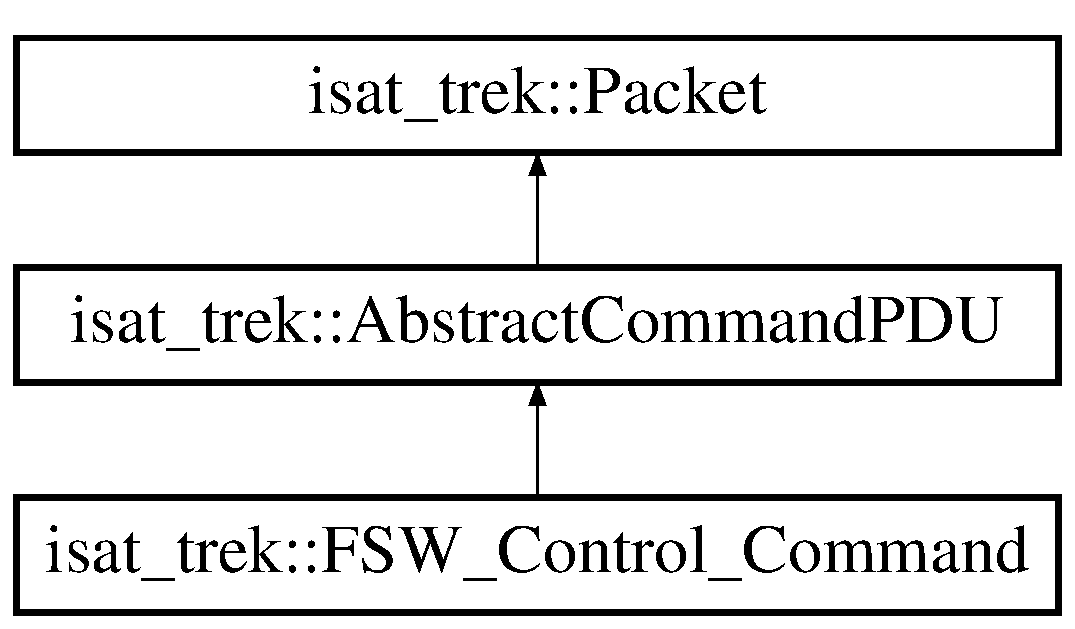
\includegraphics[height=3.000000cm]{classisat__trek_1_1_f_s_w___control___command}
\end{center}
\end{figure}
\subsection*{Public Member Functions}
\begin{DoxyCompactItemize}
\item 
bool \hyperlink{classisat__trek_1_1_f_s_w___control___command_a53c2b5279e7d4db07b1d715593b5b5fe}{from\+Bytes} (Byte\+Buffer \&buf)
\item 
bool \hyperlink{classisat__trek_1_1_f_s_w___control___command_ada517ac287c68e7a85bf600f2152a934}{to\+Bytes} (Byte\+Buffer \&buf)
\end{DoxyCompactItemize}
\subsection*{Public Attributes}
\begin{DoxyCompactItemize}
\item 
int {\bfseries command} = 0\hypertarget{classisat__trek_1_1_f_s_w___control___command_a96f5a05311f108f0ebcf07e53905b4cf}{}\label{classisat__trek_1_1_f_s_w___control___command_a96f5a05311f108f0ebcf07e53905b4cf}

\end{DoxyCompactItemize}


\subsection{Detailed Description}
X\+XX\+: Replace with real description in isat.\+pdu file. 

\subsection{Member Function Documentation}
\index{isat\+\_\+trek\+::\+F\+S\+W\+\_\+\+Control\+\_\+\+Command@{isat\+\_\+trek\+::\+F\+S\+W\+\_\+\+Control\+\_\+\+Command}!from\+Bytes@{from\+Bytes}}
\index{from\+Bytes@{from\+Bytes}!isat\+\_\+trek\+::\+F\+S\+W\+\_\+\+Control\+\_\+\+Command@{isat\+\_\+trek\+::\+F\+S\+W\+\_\+\+Control\+\_\+\+Command}}
\subsubsection[{\texorpdfstring{from\+Bytes(\+Byte\+Buffer \&buf)}{fromBytes(ByteBuffer &buf)}}]{\setlength{\rightskip}{0pt plus 5cm}bool isat\+\_\+trek\+::\+F\+S\+W\+\_\+\+Control\+\_\+\+Command\+::from\+Bytes (
\begin{DoxyParamCaption}
\item[{Byte\+Buffer \&}]{buf}
\end{DoxyParamCaption}
)\hspace{0.3cm}{\ttfamily [virtual]}}\hypertarget{classisat__trek_1_1_f_s_w___control___command_a53c2b5279e7d4db07b1d715593b5b5fe}{}\label{classisat__trek_1_1_f_s_w___control___command_a53c2b5279e7d4db07b1d715593b5b5fe}
Populate the header and command fields from the data in buf.

\begin{DoxyReturn}{Returns}
true if successful. 
\end{DoxyReturn}


Implements \hyperlink{classisat__trek_1_1_packet}{isat\+\_\+trek\+::\+Packet}.

\index{isat\+\_\+trek\+::\+F\+S\+W\+\_\+\+Control\+\_\+\+Command@{isat\+\_\+trek\+::\+F\+S\+W\+\_\+\+Control\+\_\+\+Command}!to\+Bytes@{to\+Bytes}}
\index{to\+Bytes@{to\+Bytes}!isat\+\_\+trek\+::\+F\+S\+W\+\_\+\+Control\+\_\+\+Command@{isat\+\_\+trek\+::\+F\+S\+W\+\_\+\+Control\+\_\+\+Command}}
\subsubsection[{\texorpdfstring{to\+Bytes(\+Byte\+Buffer \&buf)}{toBytes(ByteBuffer &buf)}}]{\setlength{\rightskip}{0pt plus 5cm}bool isat\+\_\+trek\+::\+F\+S\+W\+\_\+\+Control\+\_\+\+Command\+::to\+Bytes (
\begin{DoxyParamCaption}
\item[{Byte\+Buffer \&}]{buf}
\end{DoxyParamCaption}
)\hspace{0.3cm}{\ttfamily [virtual]}}\hypertarget{classisat__trek_1_1_f_s_w___control___command_ada517ac287c68e7a85bf600f2152a934}{}\label{classisat__trek_1_1_f_s_w___control___command_ada517ac287c68e7a85bf600f2152a934}
Create the binary representation of this instance in the specified buffer.

\begin{DoxyReturn}{Returns}
true if successful. 
\end{DoxyReturn}


Implements \hyperlink{classisat__trek_1_1_packet}{isat\+\_\+trek\+::\+Packet}.



The documentation for this class was generated from the following files\+:\begin{DoxyCompactItemize}
\item 
/home/riley/work/fsw/src/isatgs/\+B\+A\+R\+Co\+Mm\+S/src/dependencies/trek/command/F\+S\+W\+\_\+\+Control\+\_\+\+Command.\+h\item 
/home/riley/work/fsw/src/isatgs/\+B\+A\+R\+Co\+Mm\+S/src/dependencies/trek/command/F\+S\+W\+\_\+\+Control\+\_\+\+Command.\+cpp\end{DoxyCompactItemize}

\hypertarget{class_f_s_w_item}{}\section{F\+S\+W\+Item Class Reference}
\label{class_f_s_w_item}\index{F\+S\+W\+Item@{F\+S\+W\+Item}}
Inheritance diagram for F\+S\+W\+Item\+:\begin{figure}[H]
\begin{center}
\leavevmode
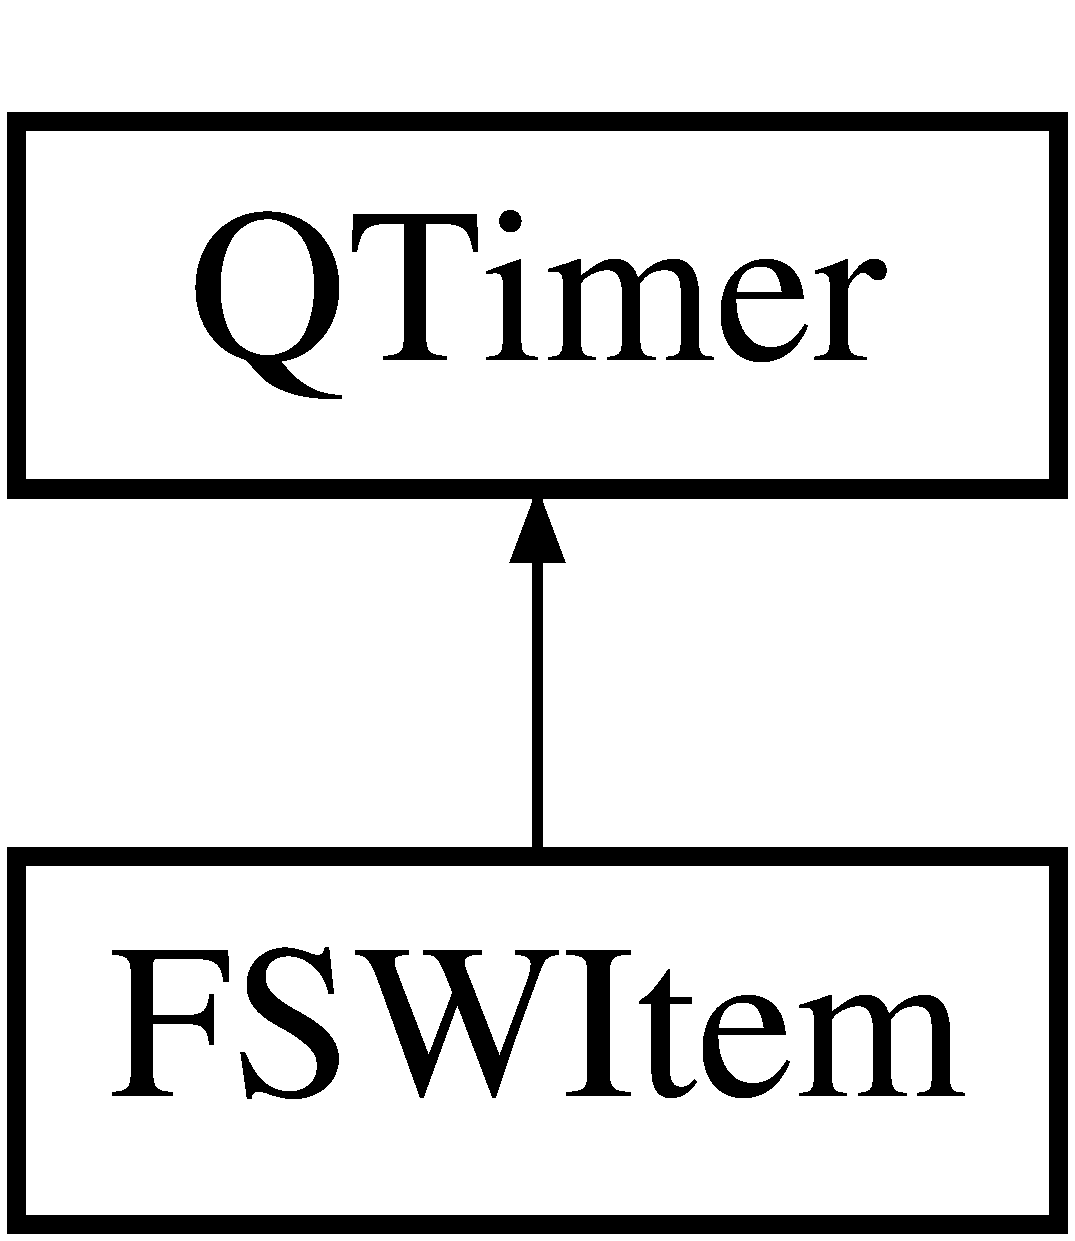
\includegraphics[height=2.000000cm]{class_f_s_w_item}
\end{center}
\end{figure}
\subsection*{Public Slots}
\begin{DoxyCompactItemize}
\item 
void {\bfseries flag\+Yellow} ()\hypertarget{class_f_s_w_item_acc52e02c28314bbf9a7e98a12ad56162}{}\label{class_f_s_w_item_acc52e02c28314bbf9a7e98a12ad56162}

\item 
void {\bfseries flag\+Orange} ()\hypertarget{class_f_s_w_item_a05d797b563d03bdacbee358dfbb5778c}{}\label{class_f_s_w_item_a05d797b563d03bdacbee358dfbb5778c}

\item 
void {\bfseries flag\+Red} ()\hypertarget{class_f_s_w_item_a2068b63b9ca60ade182b7196f58ac3d5}{}\label{class_f_s_w_item_a2068b63b9ca60ade182b7196f58ac3d5}

\end{DoxyCompactItemize}
\subsection*{Public Member Functions}
\begin{DoxyCompactItemize}
\item 
{\bfseries F\+S\+W\+Item} (int apid, int id)\hypertarget{class_f_s_w_item_ab9b10192b77e8bab50b32c2fa3f30f4a}{}\label{class_f_s_w_item_ab9b10192b77e8bab50b32c2fa3f30f4a}

\item 
void {\bfseries add\+Child} (Q\+Color color, Q\+String text, Q\+Color top\+Color)\hypertarget{class_f_s_w_item_a19d23044c2a111c840752fc230484696}{}\label{class_f_s_w_item_a19d23044c2a111c840752fc230484696}

\item 
void {\bfseries disconnect\+Timers} ()\hypertarget{class_f_s_w_item_abf98dcc7cbe4868777545867cd5bfd3d}{}\label{class_f_s_w_item_abf98dcc7cbe4868777545867cd5bfd3d}

\end{DoxyCompactItemize}
\subsection*{Public Attributes}
\begin{DoxyCompactItemize}
\item 
int {\bfseries command}\hypertarget{class_f_s_w_item_a13a256093f08ca67d69b68ddfca7c099}{}\label{class_f_s_w_item_a13a256093f08ca67d69b68ddfca7c099}

\item 
int {\bfseries fsw\+Tree\+Num}\hypertarget{class_f_s_w_item_ac19e1c46496274ab4f4fdca5e29464b6}{}\label{class_f_s_w_item_ac19e1c46496274ab4f4fdca5e29464b6}

\item 
Q\+Date\+Time {\bfseries start\+Time}\hypertarget{class_f_s_w_item_a0801d1ed513b828d83099bd86640913b}{}\label{class_f_s_w_item_a0801d1ed513b828d83099bd86640913b}

\item 
Q\+Date\+Time {\bfseries finished\+Time}\hypertarget{class_f_s_w_item_a53d42af2d29472d8dcd85392f8d89ede}{}\label{class_f_s_w_item_a53d42af2d29472d8dcd85392f8d89ede}

\item 
int {\bfseries elapsed\+Time}\hypertarget{class_f_s_w_item_a09eca3db2340afdb33ae4deffc8f597a}{}\label{class_f_s_w_item_a09eca3db2340afdb33ae4deffc8f597a}

\item 
int {\bfseries status}\hypertarget{class_f_s_w_item_a0966a2b54240520ec0008f5167716912}{}\label{class_f_s_w_item_a0966a2b54240520ec0008f5167716912}

\item 
bool {\bfseries finished}\hypertarget{class_f_s_w_item_adf25d4aa3a24bac7a9d9c65bb92d40f8}{}\label{class_f_s_w_item_adf25d4aa3a24bac7a9d9c65bb92d40f8}

\item 
Q\+Tree\+Widget\+Item $\ast$ {\bfseries top\+Level\+Item} = new Q\+Tree\+Widget\+Item()\hypertarget{class_f_s_w_item_a1aec32aefd792eefad9933cde4a9015a}{}\label{class_f_s_w_item_a1aec32aefd792eefad9933cde4a9015a}

\item 
Q\+Tree\+Widget\+Item $\ast$ {\bfseries cmd\+Seq\+Id} = new Q\+Tree\+Widget\+Item()\hypertarget{class_f_s_w_item_a528172e13eb4085704a426f7a6a8e12b}{}\label{class_f_s_w_item_a528172e13eb4085704a426f7a6a8e12b}

\item 
Q\+Tree\+Widget\+Item $\ast$ {\bfseries time} = new Q\+Tree\+Widget\+Item()\hypertarget{class_f_s_w_item_a5d3a49aa680e6711aa35ebc31ab60823}{}\label{class_f_s_w_item_a5d3a49aa680e6711aa35ebc31ab60823}

\item 
Q\+Color {\bfseries red} = Q\+Color(255, 85, 85, 160)\hypertarget{class_f_s_w_item_a95ced7f596fe9cb5d8664ec78d19f1c4}{}\label{class_f_s_w_item_a95ced7f596fe9cb5d8664ec78d19f1c4}

\item 
Q\+Color {\bfseries orange} = Q\+Color(255, 154, 53, 145)\hypertarget{class_f_s_w_item_a8c3e75732efc779eecb1ddf917e2ac22}{}\label{class_f_s_w_item_a8c3e75732efc779eecb1ddf917e2ac22}

\item 
Q\+Color {\bfseries yellow} = Q\+Color(255, 255, 102, 168)\hypertarget{class_f_s_w_item_a105e2f7856344cf2d5a2e55b52d9774e}{}\label{class_f_s_w_item_a105e2f7856344cf2d5a2e55b52d9774e}

\item 
Q\+Color {\bfseries green} = Q\+Color(147, 249, 117, 172)\hypertarget{class_f_s_w_item_a202a326db3907990197f73cf3ccbb309}{}\label{class_f_s_w_item_a202a326db3907990197f73cf3ccbb309}

\item 
Q\+Color {\bfseries none} = Q\+Color(30, 30, 30)\hypertarget{class_f_s_w_item_a63323f688160ea6bd847add899c3cf9f}{}\label{class_f_s_w_item_a63323f688160ea6bd847add899c3cf9f}

\item 
Q\+Color {\bfseries white} = Q\+Color(205, 201, 201)\hypertarget{class_f_s_w_item_a7cbb793761fa42eb155bc1cf9ba20c41}{}\label{class_f_s_w_item_a7cbb793761fa42eb155bc1cf9ba20c41}

\item 
Q\+Color {\bfseries black} = Q\+Color(0, 0, 0)\hypertarget{class_f_s_w_item_aae0025b90a36ae919448e7ba51601258}{}\label{class_f_s_w_item_aae0025b90a36ae919448e7ba51601258}

\item 
Q\+List$<$ Q\+Tree\+Widget\+Item $\ast$ $>$ {\bfseries children}\hypertarget{class_f_s_w_item_ae5c3a8e3bbf01dc07ef3c7d39838fb38}{}\label{class_f_s_w_item_ae5c3a8e3bbf01dc07ef3c7d39838fb38}

\item 
Q\+Timer $\ast$ {\bfseries timer1} = new Q\+Timer()\hypertarget{class_f_s_w_item_a6e6d442fadc7aeae3849208aa3470301}{}\label{class_f_s_w_item_a6e6d442fadc7aeae3849208aa3470301}

\item 
Q\+Timer $\ast$ {\bfseries timer2} = new Q\+Timer()\hypertarget{class_f_s_w_item_ab6a9b04aaabcfd50e9cf04e7d235f1f4}{}\label{class_f_s_w_item_ab6a9b04aaabcfd50e9cf04e7d235f1f4}

\item 
Q\+Timer $\ast$ {\bfseries timer3} = new Q\+Timer()\hypertarget{class_f_s_w_item_a6064384f266ecacff16313d8de945f2a}{}\label{class_f_s_w_item_a6064384f266ecacff16313d8de945f2a}

\item 
int {\bfseries timer1\+Length} = 5000\hypertarget{class_f_s_w_item_aea0a9360998d04d7455e9efbee2a5099}{}\label{class_f_s_w_item_aea0a9360998d04d7455e9efbee2a5099}

\item 
int {\bfseries timer2\+Length} = 10000\hypertarget{class_f_s_w_item_a064330928c1e8265d90961b077995ebf}{}\label{class_f_s_w_item_a064330928c1e8265d90961b077995ebf}

\item 
int {\bfseries timer3\+Length} = 15000\hypertarget{class_f_s_w_item_aebcbc36e1d1e77f417c07b31585d93ab}{}\label{class_f_s_w_item_aebcbc36e1d1e77f417c07b31585d93ab}

\item 
Q\+String {\bfseries timer1\+Label} = \char`\"{}5 seconds\char`\"{}\hypertarget{class_f_s_w_item_a6e4e31323b974838181003d05709ebfa}{}\label{class_f_s_w_item_a6e4e31323b974838181003d05709ebfa}

\item 
Q\+String {\bfseries timer2\+Label} = \char`\"{}10 seconds\char`\"{}\hypertarget{class_f_s_w_item_a9ca97d850590fc36ccde80101626e6da}{}\label{class_f_s_w_item_a9ca97d850590fc36ccde80101626e6da}

\item 
Q\+String {\bfseries timer3\+Label} = \char`\"{}15+ seconds\char`\"{}\hypertarget{class_f_s_w_item_a0cf5f4881f02abf482a5a897f38dd061}{}\label{class_f_s_w_item_a0cf5f4881f02abf482a5a897f38dd061}

\end{DoxyCompactItemize}


The documentation for this class was generated from the following files\+:\begin{DoxyCompactItemize}
\item 
/home/riley/work/fsw/src/isatgs/\+B\+A\+R\+Co\+Mm\+S/src/modules/\+B\+A\+R\+Co\+Mm\+S\+\_\+\+Bulletin/fswitem.\+h\item 
/home/riley/work/fsw/src/isatgs/\+B\+A\+R\+Co\+Mm\+S/src/modules/\+B\+A\+R\+Co\+Mm\+S\+\_\+\+Bulletin/fswitem.\+cpp\end{DoxyCompactItemize}

\hypertarget{classisat__trek_1_1_f_s_w_reboot___command}{}\section{isat\+\_\+trek\+:\+:F\+S\+W\+Reboot\+\_\+\+Command Class Reference}
\label{classisat__trek_1_1_f_s_w_reboot___command}\index{isat\+\_\+trek\+::\+F\+S\+W\+Reboot\+\_\+\+Command@{isat\+\_\+trek\+::\+F\+S\+W\+Reboot\+\_\+\+Command}}


{\ttfamily \#include $<$F\+S\+W\+Reboot\+\_\+\+Command.\+h$>$}

Inheritance diagram for isat\+\_\+trek\+:\+:F\+S\+W\+Reboot\+\_\+\+Command\+:\begin{figure}[H]
\begin{center}
\leavevmode
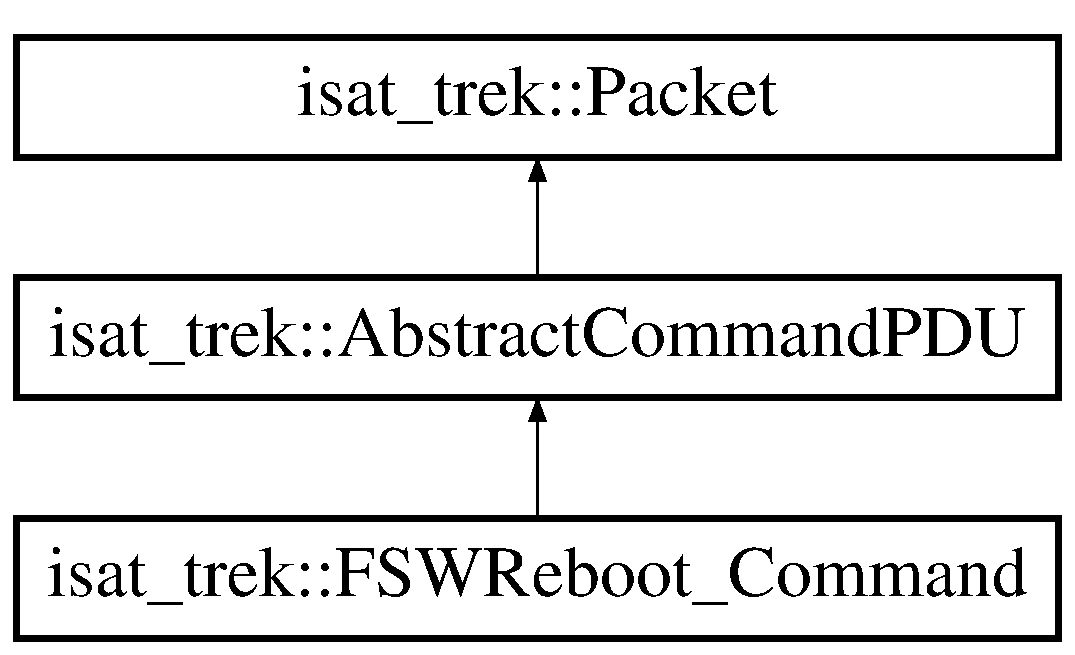
\includegraphics[height=3.000000cm]{classisat__trek_1_1_f_s_w_reboot___command}
\end{center}
\end{figure}
\subsection*{Public Member Functions}
\begin{DoxyCompactItemize}
\item 
bool \hyperlink{classisat__trek_1_1_f_s_w_reboot___command_a62441693935ded26f0bcf12081d9c21f}{from\+Bytes} (Byte\+Buffer \&buf)
\item 
bool \hyperlink{classisat__trek_1_1_f_s_w_reboot___command_a259ced73a3f10892df89015e7fa94868}{to\+Bytes} (Byte\+Buffer \&buf)
\end{DoxyCompactItemize}
\subsection*{Additional Inherited Members}


\subsection{Detailed Description}
X\+XX\+: Replace with real description in isat.\+pdu file. 

\subsection{Member Function Documentation}
\index{isat\+\_\+trek\+::\+F\+S\+W\+Reboot\+\_\+\+Command@{isat\+\_\+trek\+::\+F\+S\+W\+Reboot\+\_\+\+Command}!from\+Bytes@{from\+Bytes}}
\index{from\+Bytes@{from\+Bytes}!isat\+\_\+trek\+::\+F\+S\+W\+Reboot\+\_\+\+Command@{isat\+\_\+trek\+::\+F\+S\+W\+Reboot\+\_\+\+Command}}
\subsubsection[{\texorpdfstring{from\+Bytes(\+Byte\+Buffer \&buf)}{fromBytes(ByteBuffer &buf)}}]{\setlength{\rightskip}{0pt plus 5cm}bool isat\+\_\+trek\+::\+F\+S\+W\+Reboot\+\_\+\+Command\+::from\+Bytes (
\begin{DoxyParamCaption}
\item[{Byte\+Buffer \&}]{buf}
\end{DoxyParamCaption}
)\hspace{0.3cm}{\ttfamily [virtual]}}\hypertarget{classisat__trek_1_1_f_s_w_reboot___command_a62441693935ded26f0bcf12081d9c21f}{}\label{classisat__trek_1_1_f_s_w_reboot___command_a62441693935ded26f0bcf12081d9c21f}
Populate the header and command fields from the data in buf.

\begin{DoxyReturn}{Returns}
true if successful. 
\end{DoxyReturn}


Implements \hyperlink{classisat__trek_1_1_packet}{isat\+\_\+trek\+::\+Packet}.

\index{isat\+\_\+trek\+::\+F\+S\+W\+Reboot\+\_\+\+Command@{isat\+\_\+trek\+::\+F\+S\+W\+Reboot\+\_\+\+Command}!to\+Bytes@{to\+Bytes}}
\index{to\+Bytes@{to\+Bytes}!isat\+\_\+trek\+::\+F\+S\+W\+Reboot\+\_\+\+Command@{isat\+\_\+trek\+::\+F\+S\+W\+Reboot\+\_\+\+Command}}
\subsubsection[{\texorpdfstring{to\+Bytes(\+Byte\+Buffer \&buf)}{toBytes(ByteBuffer &buf)}}]{\setlength{\rightskip}{0pt plus 5cm}bool isat\+\_\+trek\+::\+F\+S\+W\+Reboot\+\_\+\+Command\+::to\+Bytes (
\begin{DoxyParamCaption}
\item[{Byte\+Buffer \&}]{buf}
\end{DoxyParamCaption}
)\hspace{0.3cm}{\ttfamily [virtual]}}\hypertarget{classisat__trek_1_1_f_s_w_reboot___command_a259ced73a3f10892df89015e7fa94868}{}\label{classisat__trek_1_1_f_s_w_reboot___command_a259ced73a3f10892df89015e7fa94868}
Create the binary representation of this instance in the specified buffer.

\begin{DoxyReturn}{Returns}
true if successful. 
\end{DoxyReturn}


Implements \hyperlink{classisat__trek_1_1_packet}{isat\+\_\+trek\+::\+Packet}.



The documentation for this class was generated from the following files\+:\begin{DoxyCompactItemize}
\item 
/home/riley/work/fsw/src/isatgs/\+B\+A\+R\+Co\+Mm\+S/src/dependencies/trek/command/F\+S\+W\+Reboot\+\_\+\+Command.\+h\item 
/home/riley/work/fsw/src/isatgs/\+B\+A\+R\+Co\+Mm\+S/src/dependencies/trek/command/F\+S\+W\+Reboot\+\_\+\+Command.\+cpp\end{DoxyCompactItemize}

\hypertarget{classisat__trek_1_1_f_s_w_restart___command}{}\section{isat\+\_\+trek\+:\+:F\+S\+W\+Restart\+\_\+\+Command Class Reference}
\label{classisat__trek_1_1_f_s_w_restart___command}\index{isat\+\_\+trek\+::\+F\+S\+W\+Restart\+\_\+\+Command@{isat\+\_\+trek\+::\+F\+S\+W\+Restart\+\_\+\+Command}}


{\ttfamily \#include $<$F\+S\+W\+Restart\+\_\+\+Command.\+h$>$}

Inheritance diagram for isat\+\_\+trek\+:\+:F\+S\+W\+Restart\+\_\+\+Command\+:\begin{figure}[H]
\begin{center}
\leavevmode
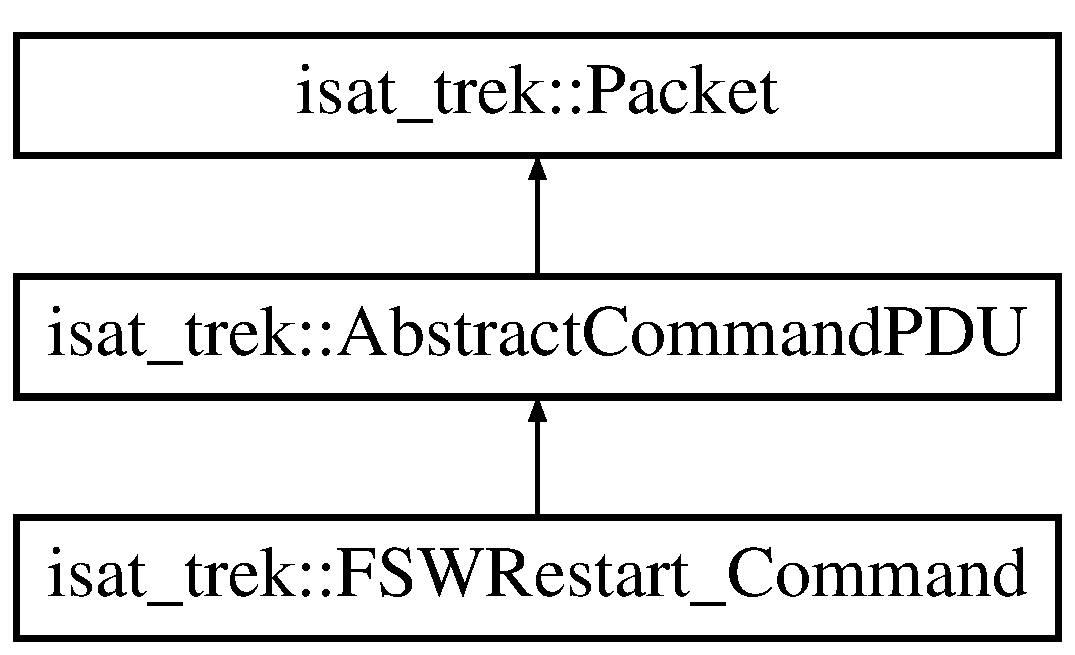
\includegraphics[height=3.000000cm]{classisat__trek_1_1_f_s_w_restart___command}
\end{center}
\end{figure}
\subsection*{Public Member Functions}
\begin{DoxyCompactItemize}
\item 
bool \hyperlink{classisat__trek_1_1_f_s_w_restart___command_a743dc34ed5eff41c806566e1d9a9892f}{from\+Bytes} (Byte\+Buffer \&buf)
\item 
bool \hyperlink{classisat__trek_1_1_f_s_w_restart___command_a40498621916cbf4e90f3ed16cb23338e}{to\+Bytes} (Byte\+Buffer \&buf)
\end{DoxyCompactItemize}
\subsection*{Additional Inherited Members}


\subsection{Detailed Description}
X\+XX\+: Replace with real description in isat.\+pdu file. 

\subsection{Member Function Documentation}
\index{isat\+\_\+trek\+::\+F\+S\+W\+Restart\+\_\+\+Command@{isat\+\_\+trek\+::\+F\+S\+W\+Restart\+\_\+\+Command}!from\+Bytes@{from\+Bytes}}
\index{from\+Bytes@{from\+Bytes}!isat\+\_\+trek\+::\+F\+S\+W\+Restart\+\_\+\+Command@{isat\+\_\+trek\+::\+F\+S\+W\+Restart\+\_\+\+Command}}
\subsubsection[{\texorpdfstring{from\+Bytes(\+Byte\+Buffer \&buf)}{fromBytes(ByteBuffer &buf)}}]{\setlength{\rightskip}{0pt plus 5cm}bool isat\+\_\+trek\+::\+F\+S\+W\+Restart\+\_\+\+Command\+::from\+Bytes (
\begin{DoxyParamCaption}
\item[{Byte\+Buffer \&}]{buf}
\end{DoxyParamCaption}
)\hspace{0.3cm}{\ttfamily [virtual]}}\hypertarget{classisat__trek_1_1_f_s_w_restart___command_a743dc34ed5eff41c806566e1d9a9892f}{}\label{classisat__trek_1_1_f_s_w_restart___command_a743dc34ed5eff41c806566e1d9a9892f}
Populate the header and command fields from the data in buf.

\begin{DoxyReturn}{Returns}
true if successful. 
\end{DoxyReturn}


Implements \hyperlink{classisat__trek_1_1_packet}{isat\+\_\+trek\+::\+Packet}.

\index{isat\+\_\+trek\+::\+F\+S\+W\+Restart\+\_\+\+Command@{isat\+\_\+trek\+::\+F\+S\+W\+Restart\+\_\+\+Command}!to\+Bytes@{to\+Bytes}}
\index{to\+Bytes@{to\+Bytes}!isat\+\_\+trek\+::\+F\+S\+W\+Restart\+\_\+\+Command@{isat\+\_\+trek\+::\+F\+S\+W\+Restart\+\_\+\+Command}}
\subsubsection[{\texorpdfstring{to\+Bytes(\+Byte\+Buffer \&buf)}{toBytes(ByteBuffer &buf)}}]{\setlength{\rightskip}{0pt plus 5cm}bool isat\+\_\+trek\+::\+F\+S\+W\+Restart\+\_\+\+Command\+::to\+Bytes (
\begin{DoxyParamCaption}
\item[{Byte\+Buffer \&}]{buf}
\end{DoxyParamCaption}
)\hspace{0.3cm}{\ttfamily [virtual]}}\hypertarget{classisat__trek_1_1_f_s_w_restart___command_a40498621916cbf4e90f3ed16cb23338e}{}\label{classisat__trek_1_1_f_s_w_restart___command_a40498621916cbf4e90f3ed16cb23338e}
Create the binary representation of this instance in the specified buffer.

\begin{DoxyReturn}{Returns}
true if successful. 
\end{DoxyReturn}


Implements \hyperlink{classisat__trek_1_1_packet}{isat\+\_\+trek\+::\+Packet}.



The documentation for this class was generated from the following files\+:\begin{DoxyCompactItemize}
\item 
/home/riley/work/fsw/src/isatgs/\+B\+A\+R\+Co\+Mm\+S/src/dependencies/trek/command/F\+S\+W\+Restart\+\_\+\+Command.\+h\item 
/home/riley/work/fsw/src/isatgs/\+B\+A\+R\+Co\+Mm\+S/src/dependencies/trek/command/F\+S\+W\+Restart\+\_\+\+Command.\+cpp\end{DoxyCompactItemize}

\hypertarget{structgap}{}\section{gap Struct Reference}
\label{structgap}\index{gap@{gap}}
\subsection*{Public Attributes}
\begin{DoxyCompactItemize}
\item 
u\+\_\+int\+\_\+4 {\bfseries begin}\hypertarget{structgap_a12391414ff856122bc95438776497cbd}{}\label{structgap_a12391414ff856122bc95438776497cbd}

\item 
u\+\_\+int\+\_\+4 {\bfseries end}\hypertarget{structgap_a503365cbf83e5bb8917f912403f39e3a}{}\label{structgap_a503365cbf83e5bb8917f912403f39e3a}

\item 
struct \hyperlink{structgap}{gap} $\ast$ {\bfseries next}\hypertarget{structgap_ad2570b6ec1c81c481d237cce1e195cfa}{}\label{structgap_ad2570b6ec1c81c481d237cce1e195cfa}

\end{DoxyCompactItemize}


The documentation for this struct was generated from the following file\+:\begin{DoxyCompactItemize}
\item 
/home/riley/work/fsw/src/isatgs/\+B\+A\+R\+Co\+Mm\+S/src/dependencies/\+C\+F\+D\+P/\+P\+R\+I/structures.\+h\end{DoxyCompactItemize}

\hypertarget{class_g_l_widget}{}\section{G\+L\+Widget Class Reference}
\label{class_g_l_widget}\index{G\+L\+Widget@{G\+L\+Widget}}
Inheritance diagram for G\+L\+Widget\+:\begin{figure}[H]
\begin{center}
\leavevmode
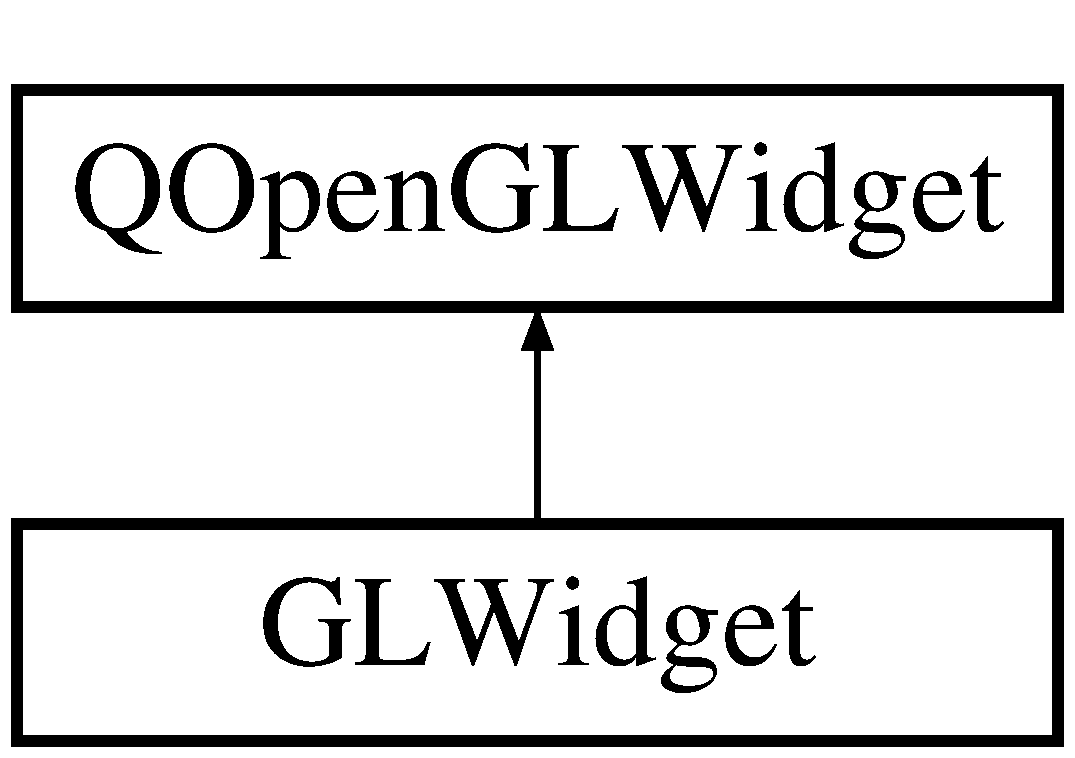
\includegraphics[height=2.000000cm]{class_g_l_widget}
\end{center}
\end{figure}
\subsection*{Public Slots}
\begin{DoxyCompactItemize}
\item 
void {\bfseries change\+Value} (int value, char $\ast$name)\hypertarget{class_g_l_widget_a7c72bab4c6a9662487718c741e6bd22d}{}\label{class_g_l_widget_a7c72bab4c6a9662487718c741e6bd22d}

\end{DoxyCompactItemize}
\subsection*{Signals}
\begin{DoxyCompactItemize}
\item 
void {\bfseries G\+L\+Startup} ()\hypertarget{class_g_l_widget_a2f91231c336a0eeb36df927f2d2840a2}{}\label{class_g_l_widget_a2f91231c336a0eeb36df927f2d2840a2}

\item 
void {\bfseries image\+Changed} (Q\+String image\+Path)\hypertarget{class_g_l_widget_a5187e72bdf07719b60bc37670bcaab04}{}\label{class_g_l_widget_a5187e72bdf07719b60bc37670bcaab04}

\end{DoxyCompactItemize}
\subsection*{Public Member Functions}
\begin{DoxyCompactItemize}
\item 
{\bfseries G\+L\+Widget} (Q\+Widget $\ast$parent=0)\hypertarget{class_g_l_widget_ab79c391c86de1ffb76f6950b49d82c0c}{}\label{class_g_l_widget_ab79c391c86de1ffb76f6950b49d82c0c}

\item 
void {\bfseries initialize\+GL} ()\hypertarget{class_g_l_widget_a7fab13e8cc9fc0730ca54c08b2c923a7}{}\label{class_g_l_widget_a7fab13e8cc9fc0730ca54c08b2c923a7}

\item 
void {\bfseries paint\+GL} ()\hypertarget{class_g_l_widget_a640b5570cb2b37724fd5b58a77339c5e}{}\label{class_g_l_widget_a640b5570cb2b37724fd5b58a77339c5e}

\item 
void {\bfseries resize\+GL} (int width, int height)\hypertarget{class_g_l_widget_ac0d2a8ecf60907a81c0d73475d851025}{}\label{class_g_l_widget_ac0d2a8ecf60907a81c0d73475d851025}

\item 
void {\bfseries load\+Texture\+Img} (Q\+String image\+Path)\hypertarget{class_g_l_widget_a1d6481cdcdaac818086d802ccfe47425}{}\label{class_g_l_widget_a1d6481cdcdaac818086d802ccfe47425}

\item 
void {\bfseries tear\+Down\+GL} ()\hypertarget{class_g_l_widget_a39c0ae6fe9b0249dd495533d2164e9b6}{}\label{class_g_l_widget_a39c0ae6fe9b0249dd495533d2164e9b6}

\item 
void {\bfseries set\+Current\+Image} (Q\+String image\+Path)\hypertarget{class_g_l_widget_ac5e85a5dd05e92833bc542545436c15b}{}\label{class_g_l_widget_ac5e85a5dd05e92833bc542545436c15b}

\end{DoxyCompactItemize}


The documentation for this class was generated from the following files\+:\begin{DoxyCompactItemize}
\item 
/home/riley/work/fsw/src/isatgs/\+B\+A\+R\+Co\+Mm\+S/src/modules/\+B\+A\+R\+Co\+Mm\+S\+\_\+\+Camera/glwidget.\+h\item 
/home/riley/work/fsw/src/isatgs/\+B\+A\+R\+Co\+Mm\+S/src/modules/\+B\+A\+R\+Co\+Mm\+S\+\_\+\+Camera/glwidget.\+cpp\end{DoxyCompactItemize}

\hypertarget{classisat__trek_1_1_g_n_c1___telemetry}{}\section{isat\+\_\+trek\+:\+:G\+N\+C1\+\_\+\+Telemetry Class Reference}
\label{classisat__trek_1_1_g_n_c1___telemetry}\index{isat\+\_\+trek\+::\+G\+N\+C1\+\_\+\+Telemetry@{isat\+\_\+trek\+::\+G\+N\+C1\+\_\+\+Telemetry}}
Inheritance diagram for isat\+\_\+trek\+:\+:G\+N\+C1\+\_\+\+Telemetry\+:\begin{figure}[H]
\begin{center}
\leavevmode
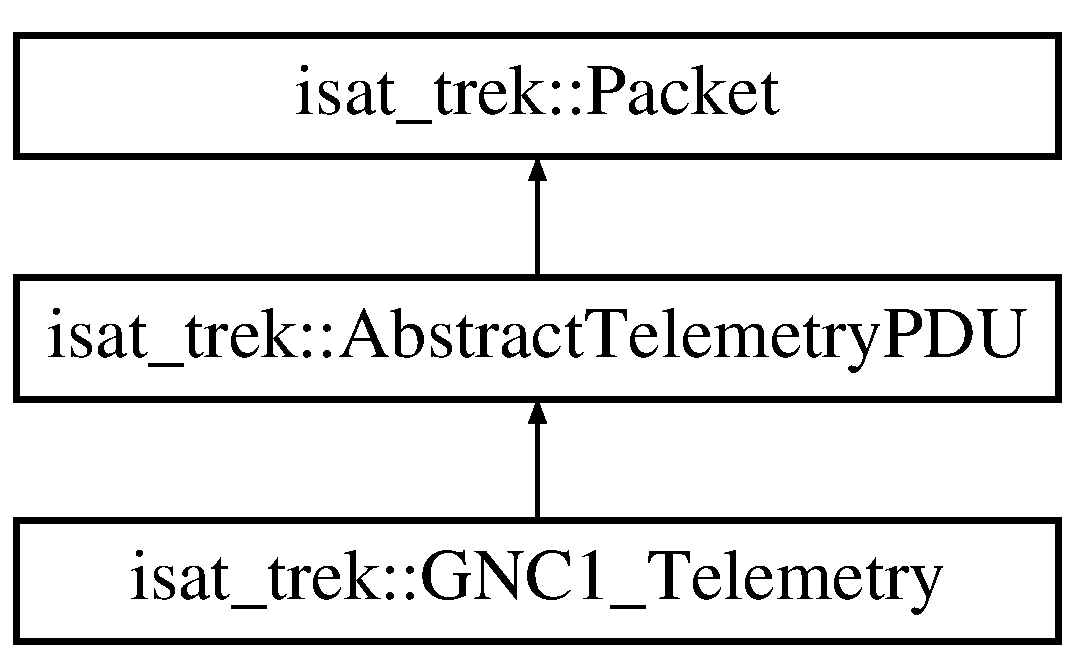
\includegraphics[height=3.000000cm]{classisat__trek_1_1_g_n_c1___telemetry}
\end{center}
\end{figure}
\subsection*{Public Member Functions}
\begin{DoxyCompactItemize}
\item 
virtual bool \hyperlink{classisat__trek_1_1_g_n_c1___telemetry_abe69f50e0b2590c99d157e1f1dcec1d8}{from\+Bytes} (Byte\+Buffer \&buf)
\item 
virtual bool \hyperlink{classisat__trek_1_1_g_n_c1___telemetry_a9b35c147802a663cfe053813986191ae}{to\+Bytes} (Byte\+Buffer \&buf)
\end{DoxyCompactItemize}
\subsection*{Public Attributes}
\begin{DoxyCompactItemize}
\item 
int {\bfseries w\+EstX}\hypertarget{classisat__trek_1_1_g_n_c1___telemetry_aa8e42979245278be69665b876db4cab5}{}\label{classisat__trek_1_1_g_n_c1___telemetry_aa8e42979245278be69665b876db4cab5}

\item 
int {\bfseries w\+EstY}\hypertarget{classisat__trek_1_1_g_n_c1___telemetry_af6de9e29237486bc962aa84a603b7ee7}{}\label{classisat__trek_1_1_g_n_c1___telemetry_af6de9e29237486bc962aa84a603b7ee7}

\item 
int {\bfseries w\+EstZ}\hypertarget{classisat__trek_1_1_g_n_c1___telemetry_a505a933641f6ab6c38ae157a20766eae}{}\label{classisat__trek_1_1_g_n_c1___telemetry_a505a933641f6ab6c38ae157a20766eae}

\item 
int {\bfseries att\+Valid}\hypertarget{classisat__trek_1_1_g_n_c1___telemetry_a66c8cc0be5dd47e1138cca6608b6dc21}{}\label{classisat__trek_1_1_g_n_c1___telemetry_a66c8cc0be5dd47e1138cca6608b6dc21}

\item 
int {\bfseries att\+Meas\+Avail}\hypertarget{classisat__trek_1_1_g_n_c1___telemetry_a44b0ec7507e04d045c29e2a14925ef76}{}\label{classisat__trek_1_1_g_n_c1___telemetry_a44b0ec7507e04d045c29e2a14925ef76}

\item 
int {\bfseries rw\+Cmd\+TorqueX}\hypertarget{classisat__trek_1_1_g_n_c1___telemetry_a0b13b4f990adffad40ed393ed60b8e5e}{}\label{classisat__trek_1_1_g_n_c1___telemetry_a0b13b4f990adffad40ed393ed60b8e5e}

\item 
int {\bfseries rw\+Cmd\+TorqueY}\hypertarget{classisat__trek_1_1_g_n_c1___telemetry_aa0bdbc340130232b420532e5f9fcf495}{}\label{classisat__trek_1_1_g_n_c1___telemetry_aa0bdbc340130232b420532e5f9fcf495}

\item 
int {\bfseries rw\+Cmd\+TorqueZ}\hypertarget{classisat__trek_1_1_g_n_c1___telemetry_ace272eed700983973dd09b4ad9220b57}{}\label{classisat__trek_1_1_g_n_c1___telemetry_ace272eed700983973dd09b4ad9220b57}

\item 
int {\bfseries trq\+Cmd\+DipoleX}\hypertarget{classisat__trek_1_1_g_n_c1___telemetry_a6b51482f86240790240078f3d7241bb4}{}\label{classisat__trek_1_1_g_n_c1___telemetry_a6b51482f86240790240078f3d7241bb4}

\item 
int {\bfseries trq\+Cmd\+DipoleY}\hypertarget{classisat__trek_1_1_g_n_c1___telemetry_a49a04e93a03636dd9f3e4f73fbd4d95d}{}\label{classisat__trek_1_1_g_n_c1___telemetry_a49a04e93a03636dd9f3e4f73fbd4d95d}

\item 
int {\bfseries trq\+Cmd\+DipoleZ}\hypertarget{classisat__trek_1_1_g_n_c1___telemetry_ad6702058bda4088d4f13e038d8fb436c}{}\label{classisat__trek_1_1_g_n_c1___telemetry_ad6702058bda4088d4f13e038d8fb436c}

\item 
int {\bfseries gnc\+Mode}\hypertarget{classisat__trek_1_1_g_n_c1___telemetry_a7eb3b64dcff3a870412359b11f0f30d2}{}\label{classisat__trek_1_1_g_n_c1___telemetry_a7eb3b64dcff3a870412359b11f0f30d2}

\item 
int {\bfseries gnc\+Submode}\hypertarget{classisat__trek_1_1_g_n_c1___telemetry_a60ce96a0e50f002350c46cb9c08289b6}{}\label{classisat__trek_1_1_g_n_c1___telemetry_a60ce96a0e50f002350c46cb9c08289b6}

\item 
int {\bfseries enable\+MM}\hypertarget{classisat__trek_1_1_g_n_c1___telemetry_aee01d886ebfeba89cd0315bae7032292}{}\label{classisat__trek_1_1_g_n_c1___telemetry_aee01d886ebfeba89cd0315bae7032292}

\item 
int {\bfseries valid\+Cmd\+Flag}\hypertarget{classisat__trek_1_1_g_n_c1___telemetry_a0de4fa66ddfc905bd16fdc8fe48b0f45}{}\label{classisat__trek_1_1_g_n_c1___telemetry_a0de4fa66ddfc905bd16fdc8fe48b0f45}

\item 
int {\bfseries nav\+Valid\+Flag}\hypertarget{classisat__trek_1_1_g_n_c1___telemetry_a1e203f5b20118db4d95e9b225bf24228}{}\label{classisat__trek_1_1_g_n_c1___telemetry_a1e203f5b20118db4d95e9b225bf24228}

\item 
int {\bfseries t\+Cur}\hypertarget{classisat__trek_1_1_g_n_c1___telemetry_a223ca16f22317b227d9ea4919259c3c7}{}\label{classisat__trek_1_1_g_n_c1___telemetry_a223ca16f22317b227d9ea4919259c3c7}

\end{DoxyCompactItemize}


\subsection{Member Function Documentation}
\index{isat\+\_\+trek\+::\+G\+N\+C1\+\_\+\+Telemetry@{isat\+\_\+trek\+::\+G\+N\+C1\+\_\+\+Telemetry}!from\+Bytes@{from\+Bytes}}
\index{from\+Bytes@{from\+Bytes}!isat\+\_\+trek\+::\+G\+N\+C1\+\_\+\+Telemetry@{isat\+\_\+trek\+::\+G\+N\+C1\+\_\+\+Telemetry}}
\subsubsection[{\texorpdfstring{from\+Bytes(\+Byte\+Buffer \&buf)}{fromBytes(ByteBuffer &buf)}}]{\setlength{\rightskip}{0pt plus 5cm}bool isat\+\_\+trek\+::\+G\+N\+C1\+\_\+\+Telemetry\+::from\+Bytes (
\begin{DoxyParamCaption}
\item[{Byte\+Buffer \&}]{buf}
\end{DoxyParamCaption}
)\hspace{0.3cm}{\ttfamily [virtual]}}\hypertarget{classisat__trek_1_1_g_n_c1___telemetry_abe69f50e0b2590c99d157e1f1dcec1d8}{}\label{classisat__trek_1_1_g_n_c1___telemetry_abe69f50e0b2590c99d157e1f1dcec1d8}
Populate the header and command fields from the data in buf.

\begin{DoxyReturn}{Returns}
true if successful. 
\end{DoxyReturn}


Implements \hyperlink{classisat__trek_1_1_packet}{isat\+\_\+trek\+::\+Packet}.

\index{isat\+\_\+trek\+::\+G\+N\+C1\+\_\+\+Telemetry@{isat\+\_\+trek\+::\+G\+N\+C1\+\_\+\+Telemetry}!to\+Bytes@{to\+Bytes}}
\index{to\+Bytes@{to\+Bytes}!isat\+\_\+trek\+::\+G\+N\+C1\+\_\+\+Telemetry@{isat\+\_\+trek\+::\+G\+N\+C1\+\_\+\+Telemetry}}
\subsubsection[{\texorpdfstring{to\+Bytes(\+Byte\+Buffer \&buf)}{toBytes(ByteBuffer &buf)}}]{\setlength{\rightskip}{0pt plus 5cm}bool isat\+\_\+trek\+::\+G\+N\+C1\+\_\+\+Telemetry\+::to\+Bytes (
\begin{DoxyParamCaption}
\item[{Byte\+Buffer \&}]{buf}
\end{DoxyParamCaption}
)\hspace{0.3cm}{\ttfamily [virtual]}}\hypertarget{classisat__trek_1_1_g_n_c1___telemetry_a9b35c147802a663cfe053813986191ae}{}\label{classisat__trek_1_1_g_n_c1___telemetry_a9b35c147802a663cfe053813986191ae}
Create the binary representation of this instance in the specified buffer.

\begin{DoxyReturn}{Returns}
true if successful. 
\end{DoxyReturn}


Implements \hyperlink{classisat__trek_1_1_packet}{isat\+\_\+trek\+::\+Packet}.



The documentation for this class was generated from the following files\+:\begin{DoxyCompactItemize}
\item 
/home/riley/work/fsw/src/isatgs/\+B\+A\+R\+Co\+Mm\+S/src/dependencies/trek/telemetry/G\+N\+C1\+\_\+\+Telemetry.\+h\item 
/home/riley/work/fsw/src/isatgs/\+B\+A\+R\+Co\+Mm\+S/src/dependencies/trek/telemetry/G\+N\+C1\+\_\+\+Telemetry.\+cpp\end{DoxyCompactItemize}

\hypertarget{classisat__utils_1_1_g_n_c_data_file}{}\section{isat\+\_\+utils\+:\+:G\+N\+C\+Data\+File Class Reference}
\label{classisat__utils_1_1_g_n_c_data_file}\index{isat\+\_\+utils\+::\+G\+N\+C\+Data\+File@{isat\+\_\+utils\+::\+G\+N\+C\+Data\+File}}


{\ttfamily \#include $<$G\+N\+C\+Data\+File.\+h$>$}

\subsection*{Public Member Functions}
\begin{DoxyCompactItemize}
\item 
bool {\bfseries open} (\hyperlink{classisat__utils_1_1_string}{String} filename)\hypertarget{classisat__utils_1_1_g_n_c_data_file_ae11b406b9dd075b2e2b043b19038569e}{}\label{classisat__utils_1_1_g_n_c_data_file_ae11b406b9dd075b2e2b043b19038569e}

\item 
bool \hyperlink{classisat__utils_1_1_g_n_c_data_file_a6a89eb1aa7ec3874cb8d1570dd590880}{get\+Line} ()
\item 
double {\bfseries get\+Double} (int column)\hypertarget{classisat__utils_1_1_g_n_c_data_file_ab22f80a46bc9cac5f7ba740b58e2eb56}{}\label{classisat__utils_1_1_g_n_c_data_file_ab22f80a46bc9cac5f7ba740b58e2eb56}

\item 
bool {\bfseries close} ()\hypertarget{classisat__utils_1_1_g_n_c_data_file_a4c16d6555f8048eaf78d429daf542cb3}{}\label{classisat__utils_1_1_g_n_c_data_file_a4c16d6555f8048eaf78d429daf542cb3}

\end{DoxyCompactItemize}


\subsection{Detailed Description}
Simple asbstraction to read and parse a comma separated value (C\+SV) file.

\hyperlink{classisat__utils_1_1_g_n_c_data_file}{G\+N\+C\+Data\+File} infile; infile.\+open(\char`\"{}foo.\+csv\char`\"{});

while(infile.\+get\+Line()) \{ int param1 = infile.\+get\+Int(26, 0); // Read column 26 as int, default value 0 double param2 = infile.\+get\+Double(14, 3.\+14); // Read column 14 as double, default value 3.\+14. \}

infile.\+close(); 

\subsection{Member Function Documentation}
\index{isat\+\_\+utils\+::\+G\+N\+C\+Data\+File@{isat\+\_\+utils\+::\+G\+N\+C\+Data\+File}!get\+Line@{get\+Line}}
\index{get\+Line@{get\+Line}!isat\+\_\+utils\+::\+G\+N\+C\+Data\+File@{isat\+\_\+utils\+::\+G\+N\+C\+Data\+File}}
\subsubsection[{\texorpdfstring{get\+Line()}{getLine()}}]{\setlength{\rightskip}{0pt plus 5cm}bool isat\+\_\+utils\+::\+G\+N\+C\+Data\+File\+::get\+Line (
\begin{DoxyParamCaption}
{}
\end{DoxyParamCaption}
)}\hypertarget{classisat__utils_1_1_g_n_c_data_file_a6a89eb1aa7ec3874cb8d1570dd590880}{}\label{classisat__utils_1_1_g_n_c_data_file_a6a89eb1aa7ec3874cb8d1570dd590880}
Reads the next line in the file and makes it available to be parsed by the get$\ast$() methods. \begin{DoxyReturn}{Returns}
false if no lines are left to read. 
\end{DoxyReturn}


The documentation for this class was generated from the following files\+:\begin{DoxyCompactItemize}
\item 
/home/riley/work/fsw/src/isatgs/\+B\+A\+R\+Co\+Mm\+S/src/dependencies/utils/G\+N\+C\+Data\+File.\+h\item 
/home/riley/work/fsw/src/isatgs/\+B\+A\+R\+Co\+Mm\+S/src/dependencies/utils/G\+N\+C\+Data\+File.\+cpp\end{DoxyCompactItemize}

\hypertarget{class_graph}{}\section{Graph Class Reference}
\label{class_graph}\index{Graph@{Graph}}
\subsection*{Classes}
\begin{DoxyCompactItemize}
\item 
struct \hyperlink{struct_graph_1_1_event_item}{Event\+Item}
\item 
struct \hyperlink{struct_graph_1_1_row}{Row}
\end{DoxyCompactItemize}
\subsection*{Public Member Functions}
\begin{DoxyCompactItemize}
\item 
void {\bfseries add\+Tree\+Item} (\hyperlink{class_b_c___d_i_t_l___s_e_v_t_r_e_e___i_t_e_m}{B\+C\+\_\+\+D\+I\+T\+L\+\_\+\+S\+E\+V\+T\+R\+E\+E\+\_\+\+I\+T\+EM} $\ast$, \hyperlink{struct_graph_1_1_event_item}{Event\+Item} $\ast$)\hypertarget{class_graph_a25b4748477c4de42374689e738beb7cd}{}\label{class_graph_a25b4748477c4de42374689e738beb7cd}

\end{DoxyCompactItemize}
\subsection*{Public Attributes}
\begin{DoxyCompactItemize}
\item 
Q\+List$<$ Q\+Tree\+Widget\+Item $\ast$ $>$ {\bfseries top\+Level\+List}\hypertarget{class_graph_adc81e96a9093f4d2885909c44ae23ab0}{}\label{class_graph_adc81e96a9093f4d2885909c44ae23ab0}

\item 
Q\+Tree\+Widget\+Item $\ast$ {\bfseries Advisory}\hypertarget{class_graph_a3d5a1c394c83271640b26f8c535a5d79}{}\label{class_graph_a3d5a1c394c83271640b26f8c535a5d79}

\item 
Q\+Tree\+Widget\+Item $\ast$ {\bfseries Caution}\hypertarget{class_graph_a4e6c9011a39cbe5065e00979c28b9bcf}{}\label{class_graph_a4e6c9011a39cbe5065e00979c28b9bcf}

\item 
Q\+Tree\+Widget\+Item $\ast$ {\bfseries Warning}\hypertarget{class_graph_a1aba958c0362b6b26215c038f4ec7b43}{}\label{class_graph_a1aba958c0362b6b26215c038f4ec7b43}

\item 
Q\+Tree\+Widget\+Item $\ast$ {\bfseries Error}\hypertarget{class_graph_a546945d6848c395d82933e0932459a56}{}\label{class_graph_a546945d6848c395d82933e0932459a56}

\item 
std\+::vector$<$ double $>$ {\bfseries grid\+LineX}\hypertarget{class_graph_aaa21fee2c958db9ce8492bc07c8429c9}{}\label{class_graph_aaa21fee2c958db9ce8492bc07c8429c9}

\item 
std\+::vector$<$ double $>$ {\bfseries grid\+LineY}\hypertarget{class_graph_a43990e5e608d45070455dbcf412514f4}{}\label{class_graph_a43990e5e608d45070455dbcf412514f4}

\item 
std\+::vector$<$ \hyperlink{struct_graph_1_1_event_item}{Event\+Item} $\ast$ $>$ {\bfseries events}\hypertarget{class_graph_a7274fc075b33d6c87ba7d40cf66b35d6}{}\label{class_graph_a7274fc075b33d6c87ba7d40cf66b35d6}

\item 
std\+::vector$<$ \hyperlink{struct_graph_1_1_row}{Row} $>$ {\bfseries rows}\hypertarget{class_graph_abf9b4e4d0ea804f9fe22a9a46c0257f7}{}\label{class_graph_abf9b4e4d0ea804f9fe22a9a46c0257f7}

\item 
uint64\+\_\+t {\bfseries low}\hypertarget{class_graph_acfd2a7064a6389a24811f45719066ea0}{}\label{class_graph_acfd2a7064a6389a24811f45719066ea0}

\item 
uint64\+\_\+t {\bfseries high}\hypertarget{class_graph_a1c1b271f69610bc76da4d5460d05b19d}{}\label{class_graph_a1c1b271f69610bc76da4d5460d05b19d}

\item 
uint64\+\_\+t {\bfseries time\+Step}\hypertarget{class_graph_aa4e40f6c15416b9df71b74ed7108e8ed}{}\label{class_graph_aa4e40f6c15416b9df71b74ed7108e8ed}

\item 
Q\+Date\+Time {\bfseries last\+Time}\hypertarget{class_graph_a7ea09f92c1d2bbd4238a091927b1a43d}{}\label{class_graph_a7ea09f92c1d2bbd4238a091927b1a43d}

\end{DoxyCompactItemize}


The documentation for this class was generated from the following files\+:\begin{DoxyCompactItemize}
\item 
/home/riley/work/fsw/src/isatgs/\+B\+A\+R\+Co\+Mm\+S/src/modules/\+B\+A\+R\+Co\+Mm\+S\+\_\+\+D\+I\+T\+L/bc\+\_\+ditl\+\_\+graph.\+h\item 
/home/riley/work/fsw/src/isatgs/\+B\+A\+R\+Co\+Mm\+S/src/modules/\+B\+A\+R\+Co\+Mm\+S\+\_\+\+D\+I\+T\+L/bc\+\_\+ditl\+\_\+graph.\+cpp\end{DoxyCompactItemize}

\hypertarget{struct_h_d_r}{}\section{H\+DR Struct Reference}
\label{struct_h_d_r}\index{H\+DR@{H\+DR}}
\subsection*{Public Attributes}
\begin{DoxyCompactItemize}
\item 
P\+D\+U\+\_\+\+T\+Y\+PE {\bfseries pdu\+\_\+type}\hypertarget{struct_h_d_r_a975e1aa5feaf254f6538550f780e7a0d}{}\label{struct_h_d_r_a975e1aa5feaf254f6538550f780e7a0d}

\item 
P\+D\+U\+\_\+\+D\+I\+R\+E\+C\+T\+I\+ON {\bfseries direction}\hypertarget{struct_h_d_r_aaf64937ea3f2d84b0f306ba01cdfeeda}{}\label{struct_h_d_r_aaf64937ea3f2d84b0f306ba01cdfeeda}

\item 
P\+D\+U\+\_\+\+M\+O\+DE {\bfseries mode}\hypertarget{struct_h_d_r_a8e1bb4224e30afd6b39d11c2b55f78f8}{}\label{struct_h_d_r_a8e1bb4224e30afd6b39d11c2b55f78f8}

\item 
boolean {\bfseries use\+\_\+crc}\hypertarget{struct_h_d_r_a093c783eee5badd07c8cbb2fa9ab50d4}{}\label{struct_h_d_r_a093c783eee5badd07c8cbb2fa9ab50d4}

\item 
\hyperlink{struct_t_r_a_n_s_a_c_t_i_o_n}{T\+R\+A\+N\+S\+A\+C\+T\+I\+ON} {\bfseries trans}\hypertarget{struct_h_d_r_a98d605a5d88ec09baaf263b5ebd929d7}{}\label{struct_h_d_r_a98d605a5d88ec09baaf263b5ebd929d7}

\item 
\hyperlink{struct_i_d}{ID} {\bfseries dest\+\_\+id}\hypertarget{struct_h_d_r_a6605b4c53823b0ecad9803c18cacb7a9}{}\label{struct_h_d_r_a6605b4c53823b0ecad9803c18cacb7a9}

\end{DoxyCompactItemize}


The documentation for this struct was generated from the following file\+:\begin{DoxyCompactItemize}
\item 
/home/riley/work/fsw/src/isatgs/\+B\+A\+R\+Co\+Mm\+S/src/dependencies/\+C\+F\+D\+P/\+P\+R\+I/structures.\+h\end{DoxyCompactItemize}

\hypertarget{classisat__trek_1_1_health_status___telemetry}{}\section{isat\+\_\+trek\+:\+:Health\+Status\+\_\+\+Telemetry Class Reference}
\label{classisat__trek_1_1_health_status___telemetry}\index{isat\+\_\+trek\+::\+Health\+Status\+\_\+\+Telemetry@{isat\+\_\+trek\+::\+Health\+Status\+\_\+\+Telemetry}}
Inheritance diagram for isat\+\_\+trek\+:\+:Health\+Status\+\_\+\+Telemetry\+:\begin{figure}[H]
\begin{center}
\leavevmode
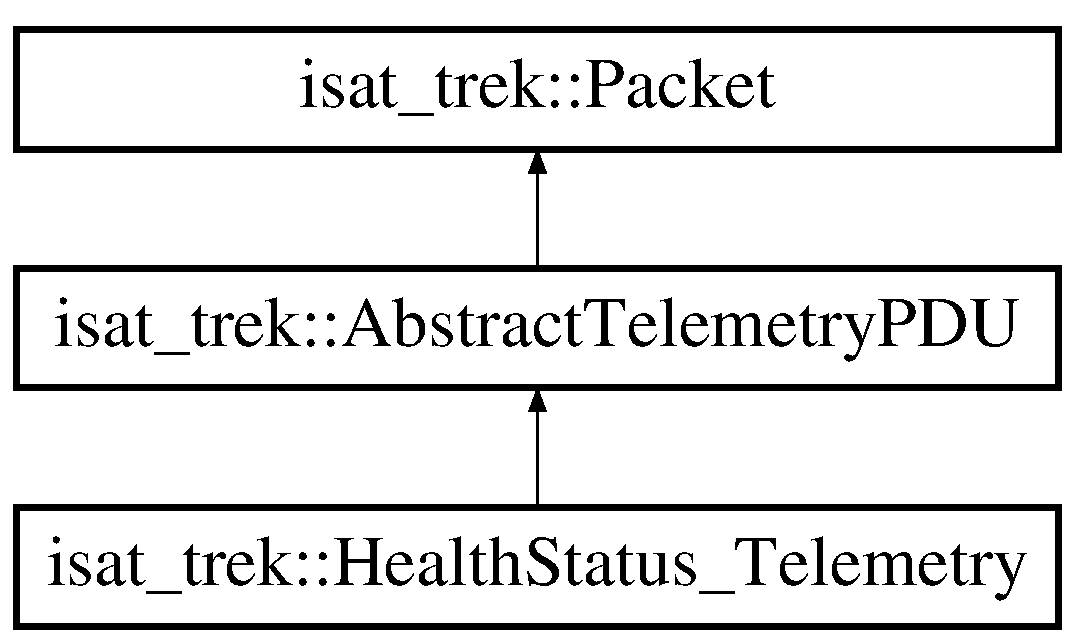
\includegraphics[height=3.000000cm]{classisat__trek_1_1_health_status___telemetry}
\end{center}
\end{figure}
\subsection*{Public Member Functions}
\begin{DoxyCompactItemize}
\item 
virtual bool \hyperlink{classisat__trek_1_1_health_status___telemetry_a119eeb6f855a7825556d519d71f31574}{from\+Bytes} (Byte\+Buffer \&buf)
\item 
virtual bool \hyperlink{classisat__trek_1_1_health_status___telemetry_ae662d21441cd159c9d31b2c8016126e4}{to\+Bytes} (Byte\+Buffer \&buf)
\end{DoxyCompactItemize}
\subsection*{Public Attributes}
\begin{DoxyCompactItemize}
\item 
int {\bfseries mode}\hypertarget{classisat__trek_1_1_health_status___telemetry_a9266d9742e07bf8fc52333817862f172}{}\label{classisat__trek_1_1_health_status___telemetry_a9266d9742e07bf8fc52333817862f172}

\item 
int {\bfseries last\+Command}\hypertarget{classisat__trek_1_1_health_status___telemetry_a6e1a5814afa24130478d970889580c92}{}\label{classisat__trek_1_1_health_status___telemetry_a6e1a5814afa24130478d970889580c92}

\item 
int {\bfseries command\+Status}\hypertarget{classisat__trek_1_1_health_status___telemetry_aa083efa90833c58a9a60724a44777372}{}\label{classisat__trek_1_1_health_status___telemetry_aa083efa90833c58a9a60724a44777372}

\item 
int {\bfseries decom\+Enabled}\hypertarget{classisat__trek_1_1_health_status___telemetry_a008416cfcf3b86b0fb7a72568212db02}{}\label{classisat__trek_1_1_health_status___telemetry_a008416cfcf3b86b0fb7a72568212db02}

\item 
int {\bfseries decom\+In\+Prog}\hypertarget{classisat__trek_1_1_health_status___telemetry_aac1d0a489eaf596598ca21087ae00761}{}\label{classisat__trek_1_1_health_status___telemetry_aac1d0a489eaf596598ca21087ae00761}

\item 
int {\bfseries comm\+Passes\+Rem}\hypertarget{classisat__trek_1_1_health_status___telemetry_a52285b4d93840c78c628232ea1606f49}{}\label{classisat__trek_1_1_health_status___telemetry_a52285b4d93840c78c628232ea1606f49}

\item 
int {\bfseries prop\+Event\+Rem}\hypertarget{classisat__trek_1_1_health_status___telemetry_ad18baa50520add1b10e6cfd3f105f90b}{}\label{classisat__trek_1_1_health_status___telemetry_ad18baa50520add1b10e6cfd3f105f90b}

\item 
int {\bfseries gnc\+Mode}\hypertarget{classisat__trek_1_1_health_status___telemetry_af1f8310e82976a586fd6f7ea97f53cf0}{}\label{classisat__trek_1_1_health_status___telemetry_af1f8310e82976a586fd6f7ea97f53cf0}

\item 
int {\bfseries cmd\+Seq\+Cnt}\hypertarget{classisat__trek_1_1_health_status___telemetry_a4bdad2f6e44412723221861b9b515f80}{}\label{classisat__trek_1_1_health_status___telemetry_a4bdad2f6e44412723221861b9b515f80}

\item 
int {\bfseries battery\+S\+OC}\hypertarget{classisat__trek_1_1_health_status___telemetry_a05854b3e791c4443840eed5e3ad2d204}{}\label{classisat__trek_1_1_health_status___telemetry_a05854b3e791c4443840eed5e3ad2d204}

\item 
int {\bfseries received\+Sig\+Str}\hypertarget{classisat__trek_1_1_health_status___telemetry_a07d499f460fe167b31efb4a8c68c8e0b}{}\label{classisat__trek_1_1_health_status___telemetry_a07d499f460fe167b31efb4a8c68c8e0b}

\item 
int {\bfseries cam\+Imgs\+Pending}\hypertarget{classisat__trek_1_1_health_status___telemetry_a5925cac49d7150e8e5a8f037d6c8f984}{}\label{classisat__trek_1_1_health_status___telemetry_a5925cac49d7150e8e5a8f037d6c8f984}

\end{DoxyCompactItemize}


\subsection{Member Function Documentation}
\index{isat\+\_\+trek\+::\+Health\+Status\+\_\+\+Telemetry@{isat\+\_\+trek\+::\+Health\+Status\+\_\+\+Telemetry}!from\+Bytes@{from\+Bytes}}
\index{from\+Bytes@{from\+Bytes}!isat\+\_\+trek\+::\+Health\+Status\+\_\+\+Telemetry@{isat\+\_\+trek\+::\+Health\+Status\+\_\+\+Telemetry}}
\subsubsection[{\texorpdfstring{from\+Bytes(\+Byte\+Buffer \&buf)}{fromBytes(ByteBuffer &buf)}}]{\setlength{\rightskip}{0pt plus 5cm}bool isat\+\_\+trek\+::\+Health\+Status\+\_\+\+Telemetry\+::from\+Bytes (
\begin{DoxyParamCaption}
\item[{Byte\+Buffer \&}]{buf}
\end{DoxyParamCaption}
)\hspace{0.3cm}{\ttfamily [virtual]}}\hypertarget{classisat__trek_1_1_health_status___telemetry_a119eeb6f855a7825556d519d71f31574}{}\label{classisat__trek_1_1_health_status___telemetry_a119eeb6f855a7825556d519d71f31574}
Populate the header and command fields from the data in buf.

\begin{DoxyReturn}{Returns}
true if successful. 
\end{DoxyReturn}


Implements \hyperlink{classisat__trek_1_1_packet}{isat\+\_\+trek\+::\+Packet}.

\index{isat\+\_\+trek\+::\+Health\+Status\+\_\+\+Telemetry@{isat\+\_\+trek\+::\+Health\+Status\+\_\+\+Telemetry}!to\+Bytes@{to\+Bytes}}
\index{to\+Bytes@{to\+Bytes}!isat\+\_\+trek\+::\+Health\+Status\+\_\+\+Telemetry@{isat\+\_\+trek\+::\+Health\+Status\+\_\+\+Telemetry}}
\subsubsection[{\texorpdfstring{to\+Bytes(\+Byte\+Buffer \&buf)}{toBytes(ByteBuffer &buf)}}]{\setlength{\rightskip}{0pt plus 5cm}bool isat\+\_\+trek\+::\+Health\+Status\+\_\+\+Telemetry\+::to\+Bytes (
\begin{DoxyParamCaption}
\item[{Byte\+Buffer \&}]{buf}
\end{DoxyParamCaption}
)\hspace{0.3cm}{\ttfamily [virtual]}}\hypertarget{classisat__trek_1_1_health_status___telemetry_ae662d21441cd159c9d31b2c8016126e4}{}\label{classisat__trek_1_1_health_status___telemetry_ae662d21441cd159c9d31b2c8016126e4}
Create the binary representation of this instance in the specified buffer.

\begin{DoxyReturn}{Returns}
true if successful. 
\end{DoxyReturn}


Implements \hyperlink{classisat__trek_1_1_packet}{isat\+\_\+trek\+::\+Packet}.



The documentation for this class was generated from the following files\+:\begin{DoxyCompactItemize}
\item 
/home/riley/work/fsw/src/isatgs/\+B\+A\+R\+Co\+Mm\+S/src/dependencies/trek/telemetry/Health\+Status\+\_\+\+Telemetry.\+h\item 
/home/riley/work/fsw/src/isatgs/\+B\+A\+R\+Co\+Mm\+S/src/dependencies/trek/telemetry/Health\+Status\+\_\+\+Telemetry.\+cpp\end{DoxyCompactItemize}

\hypertarget{class_help}{}\section{Help Class Reference}
\label{class_help}\index{Help@{Help}}
Inheritance diagram for Help\+:\begin{figure}[H]
\begin{center}
\leavevmode
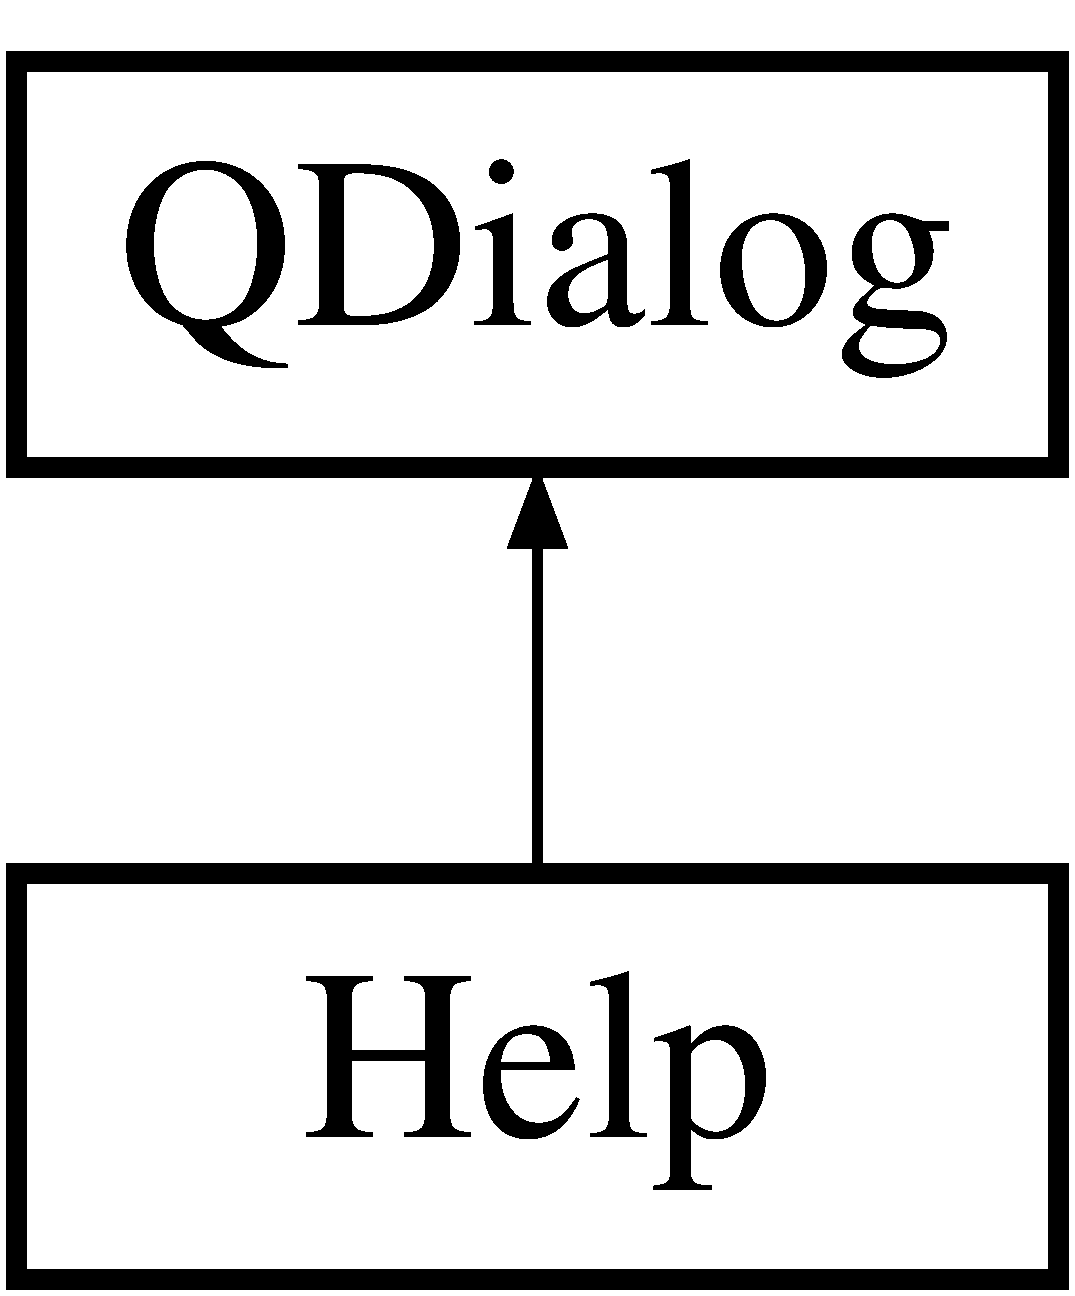
\includegraphics[height=2.000000cm]{class_help}
\end{center}
\end{figure}
\subsection*{Public Member Functions}
\begin{DoxyCompactItemize}
\item 
{\bfseries Help} (Q\+Widget $\ast$parent=0)\hypertarget{class_help_a7359f816eb2dab34e4c7017e36c9654d}{}\label{class_help_a7359f816eb2dab34e4c7017e36c9654d}

\end{DoxyCompactItemize}


The documentation for this class was generated from the following files\+:\begin{DoxyCompactItemize}
\item 
/home/riley/work/fsw/src/isatgs/\+B\+A\+R\+Co\+Mm\+S/src/modules/\+B\+A\+R\+Co\+Mm\+S\+\_\+\+C\+F\+D\+P/help.\+h\item 
/home/riley/work/fsw/src/isatgs/\+B\+A\+R\+Co\+Mm\+S/src/modules/\+B\+A\+R\+Co\+Mm\+S\+\_\+\+C\+F\+D\+P/help.\+cpp\end{DoxyCompactItemize}

\hypertarget{struct_i_d}{}\section{ID Struct Reference}
\label{struct_i_d}\index{ID@{ID}}
\subsection*{Public Attributes}
\begin{DoxyCompactItemize}
\item 
u\+\_\+int\+\_\+1 {\bfseries length}\hypertarget{struct_i_d_a7610d6b1fe7ba0b4c75614a0b0459cdc}{}\label{struct_i_d_a7610d6b1fe7ba0b4c75614a0b0459cdc}

\item 
u\+\_\+int\+\_\+1 {\bfseries value} \mbox{[}M\+A\+X\+\_\+\+I\+D\+\_\+\+L\+E\+N\+G\+TH\mbox{]}\hypertarget{struct_i_d_a0b4e0b8aeb9e93177c6ba5dfe8d0ef43}{}\label{struct_i_d_a0b4e0b8aeb9e93177c6ba5dfe8d0ef43}

\end{DoxyCompactItemize}


The documentation for this struct was generated from the following file\+:\begin{DoxyCompactItemize}
\item 
/home/riley/work/fsw/src/isatgs/\+B\+A\+R\+Co\+Mm\+S/src/dependencies/\+C\+F\+D\+P/\+P\+U\+B/cfdp\+\_\+data\+\_\+structures.\+h\end{DoxyCompactItemize}

\hypertarget{class_item}{}\section{Item Class Reference}
\label{class_item}\index{Item@{Item}}
\subsection*{Public Member Functions}
\begin{DoxyCompactItemize}
\item 
{\bfseries Item} (Q\+String trans\+Num, Q\+String class\+Num, Q\+String name, Q\+String size, float size\+Float, Q\+String node)\hypertarget{class_item_a114c7c3f92e1a1fc0e47bc02220a85cf}{}\label{class_item_a114c7c3f92e1a1fc0e47bc02220a85cf}

\item 
int {\bfseries add\+Child} (int column, Q\+Color color, Q\+String text, Q\+Icon icon)\hypertarget{class_item_a1141921aa77d1b1a314b892aeeda89dd}{}\label{class_item_a1141921aa77d1b1a314b892aeeda89dd}

\item 
void {\bfseries add\+Grand\+Child} (int parent, int column, Q\+String text)\hypertarget{class_item_aef32096d890554c8630818ad5a7a05d8}{}\label{class_item_aef32096d890554c8630818ad5a7a05d8}

\item 
Q\+String {\bfseries time} ()\hypertarget{class_item_a488a39cca0c2600cc0f99dbf0a42de32}{}\label{class_item_a488a39cca0c2600cc0f99dbf0a42de32}

\end{DoxyCompactItemize}
\subsection*{Public Attributes}
\begin{DoxyCompactItemize}
\item 
Q\+String {\bfseries tree\+Num}\hypertarget{class_item_ab51701536fec3a1a7ae5e9a71b0a5bd8}{}\label{class_item_ab51701536fec3a1a7ae5e9a71b0a5bd8}

\item 
Q\+String {\bfseries file\+Name}\hypertarget{class_item_a18d1b125537b31e3d1fa387437f5f499}{}\label{class_item_a18d1b125537b31e3d1fa387437f5f499}

\item 
Q\+Date\+Time {\bfseries start\+Time}\hypertarget{class_item_a8b9b94514b13ac3f16c4aea0e185abe6}{}\label{class_item_a8b9b94514b13ac3f16c4aea0e185abe6}

\item 
float {\bfseries file\+Size}\hypertarget{class_item_a7af91f5e63a1b6ca2218ea0872809f73}{}\label{class_item_a7af91f5e63a1b6ca2218ea0872809f73}

\item 
int {\bfseries status}\hypertarget{class_item_a7525a60123ccfc3b8cbf5ab8c28ab5d5}{}\label{class_item_a7525a60123ccfc3b8cbf5ab8c28ab5d5}

\item 
Q\+Tree\+Widget\+Item $\ast$ {\bfseries top\+Level\+Item} = new Q\+Tree\+Widget\+Item()\hypertarget{class_item_a8ee4a5d86ca268da79efa4b4212829a0}{}\label{class_item_a8ee4a5d86ca268da79efa4b4212829a0}

\item 
Q\+Tree\+Widget\+Item $\ast$ {\bfseries details} = new Q\+Tree\+Widget\+Item()\hypertarget{class_item_a78fc26d1f4c47377ae26205aaebd0d8a}{}\label{class_item_a78fc26d1f4c47377ae26205aaebd0d8a}

\item 
Q\+Tree\+Widget\+Item $\ast$ {\bfseries time\+Child} = new Q\+Tree\+Widget\+Item()\hypertarget{class_item_abba8145cd950fac8341e7fa763e5fc60}{}\label{class_item_abba8145cd950fac8341e7fa763e5fc60}

\item 
Q\+Tree\+Widget\+Item $\ast$ {\bfseries trans\+Child} = new Q\+Tree\+Widget\+Item()\hypertarget{class_item_a34e563c60fd0930e94e900379e4d4864}{}\label{class_item_a34e563c60fd0930e94e900379e4d4864}

\item 
Q\+Tree\+Widget\+Item $\ast$ {\bfseries class\+Child} = new Q\+Tree\+Widget\+Item()\hypertarget{class_item_afea5c006531a31493c0564301cce1b77}{}\label{class_item_afea5c006531a31493c0564301cce1b77}

\item 
Q\+Tree\+Widget\+Item $\ast$ {\bfseries name\+Child} = new Q\+Tree\+Widget\+Item()\hypertarget{class_item_a36bee9c8e4939a2ea09f35959d92085c}{}\label{class_item_a36bee9c8e4939a2ea09f35959d92085c}

\item 
Q\+Tree\+Widget\+Item $\ast$ {\bfseries size\+Child} = new Q\+Tree\+Widget\+Item()\hypertarget{class_item_af9fdb7357f22c8bea0beaad328d039b1}{}\label{class_item_af9fdb7357f22c8bea0beaad328d039b1}

\item 
Q\+Tree\+Widget\+Item $\ast$ {\bfseries node\+Child} = new Q\+Tree\+Widget\+Item()\hypertarget{class_item_ad07e9cb0b74ac17356e8bbc6ba62df11}{}\label{class_item_ad07e9cb0b74ac17356e8bbc6ba62df11}

\item 
Q\+Color {\bfseries red} = Q\+Color(255, 85, 85, 160)\hypertarget{class_item_ae43b892650899d44450294ba6b1b2085}{}\label{class_item_ae43b892650899d44450294ba6b1b2085}

\item 
Q\+Color {\bfseries orange} = Q\+Color(255, 154, 53, 145)\hypertarget{class_item_ae7ef22a84bbb3dbf47fae44cd34e5515}{}\label{class_item_ae7ef22a84bbb3dbf47fae44cd34e5515}

\item 
Q\+Color {\bfseries yellow} = Q\+Color(255, 255, 102, 168)\hypertarget{class_item_aad644ef4f2669e8cecfd235c2ae59469}{}\label{class_item_aad644ef4f2669e8cecfd235c2ae59469}

\item 
Q\+Color {\bfseries green} = Q\+Color(147, 249, 117, 172)\hypertarget{class_item_ab01fb8623755592211b8b1c23d348858}{}\label{class_item_ab01fb8623755592211b8b1c23d348858}

\item 
Q\+Color {\bfseries none} = Q\+Color(30, 30, 30)\hypertarget{class_item_a2d25176d7c295ce4d93576b6a55086e3}{}\label{class_item_a2d25176d7c295ce4d93576b6a55086e3}

\item 
Q\+Color {\bfseries white} = Q\+Color(205, 201, 201)\hypertarget{class_item_a419222ec51284718e4885aec07420ff2}{}\label{class_item_a419222ec51284718e4885aec07420ff2}

\item 
Q\+Color {\bfseries black} = Q\+Color(0, 0, 0)\hypertarget{class_item_a49e03569bb870f97be93907a6027b35f}{}\label{class_item_a49e03569bb870f97be93907a6027b35f}

\item 
Q\+List$<$ Q\+Tree\+Widget\+Item $\ast$ $>$ {\bfseries children}\hypertarget{class_item_ac6edaa8dddd074caf70790add03f0584}{}\label{class_item_ac6edaa8dddd074caf70790add03f0584}

\end{DoxyCompactItemize}


The documentation for this class was generated from the following files\+:\begin{DoxyCompactItemize}
\item 
/home/riley/work/fsw/src/isatgs/\+B\+A\+R\+Co\+Mm\+S/src/modules/\+B\+A\+R\+Co\+Mm\+S\+\_\+\+Bulletin/item.\+h\item 
/home/riley/work/fsw/src/isatgs/\+B\+A\+R\+Co\+Mm\+S/src/modules/\+B\+A\+R\+Co\+Mm\+S\+\_\+\+Bulletin/item.\+cpp\end{DoxyCompactItemize}

\hypertarget{classlegend}{}\section{legend Class Reference}
\label{classlegend}\index{legend@{legend}}
Inheritance diagram for legend\+:\begin{figure}[H]
\begin{center}
\leavevmode
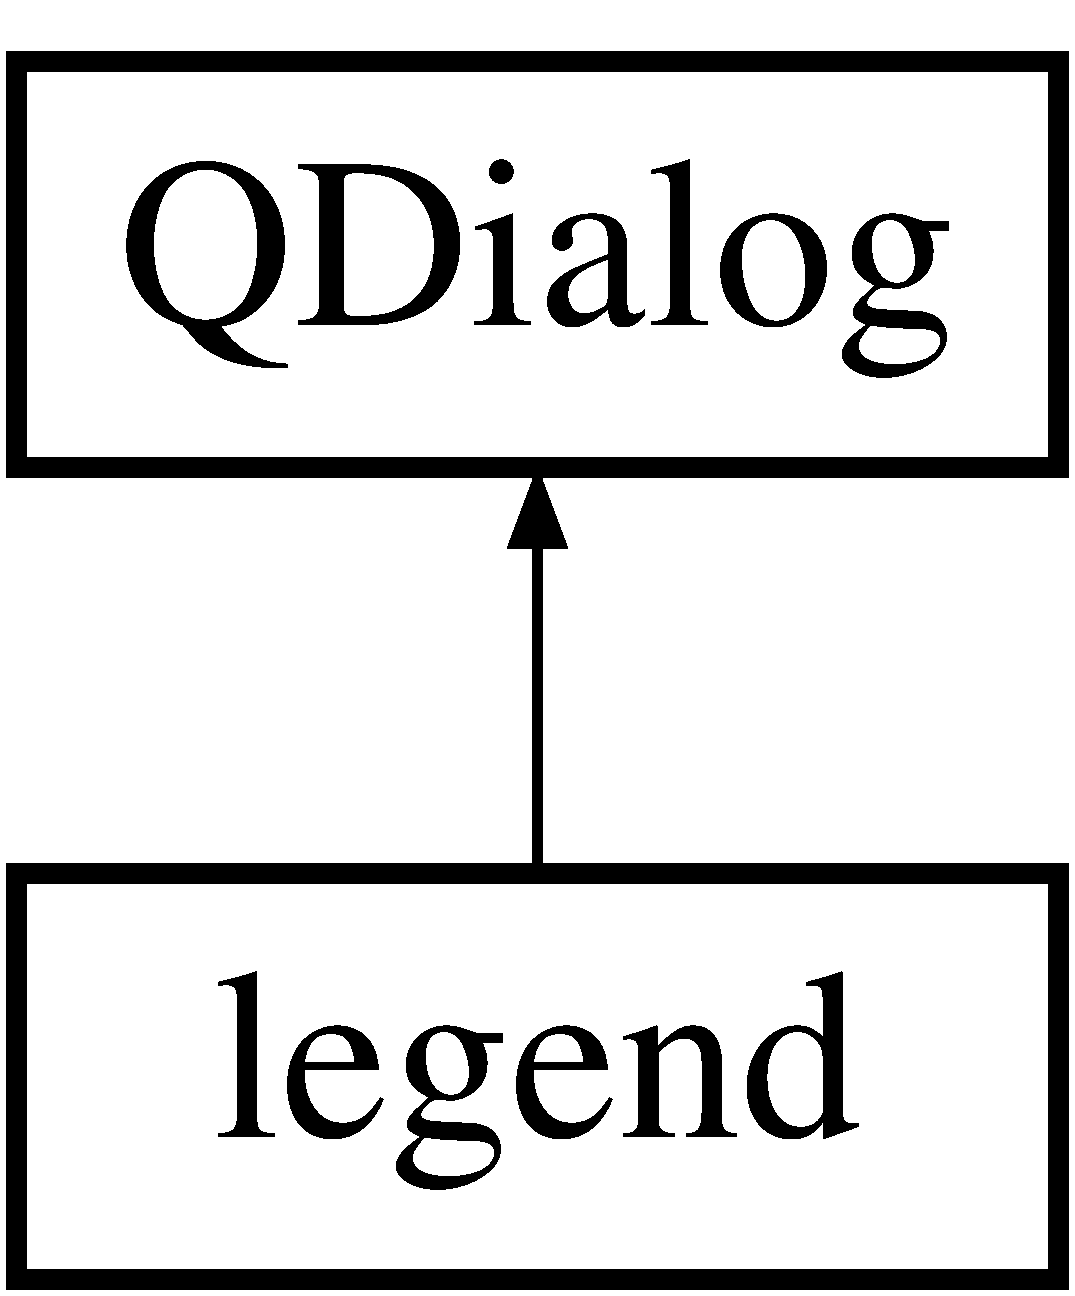
\includegraphics[height=2.000000cm]{classlegend}
\end{center}
\end{figure}
\subsection*{Public Member Functions}
\begin{DoxyCompactItemize}
\item 
{\bfseries legend} (Q\+Widget $\ast$parent=0)\hypertarget{classlegend_a5f291b6d76d65ec55d7a4aebe7ac4f09}{}\label{classlegend_a5f291b6d76d65ec55d7a4aebe7ac4f09}

\end{DoxyCompactItemize}


The documentation for this class was generated from the following files\+:\begin{DoxyCompactItemize}
\item 
/home/riley/work/fsw/src/isatgs/\+B\+A\+R\+Co\+Mm\+S/src/modules/\+B\+A\+R\+Co\+Mm\+S\+\_\+\+D\+I\+T\+L/bc\+\_\+ditl\+\_\+legend.\+h\item 
/home/riley/work/fsw/src/isatgs/\+B\+A\+R\+Co\+Mm\+S/src/modules/\+B\+A\+R\+Co\+Mm\+S\+\_\+\+D\+I\+T\+L/bc\+\_\+ditl\+\_\+legend.\+cpp\end{DoxyCompactItemize}

\hypertarget{struct_link_sim}{}\section{Link\+Sim Struct Reference}
\label{struct_link_sim}\index{Link\+Sim@{Link\+Sim}}
\subsection*{Public Attributes}
\begin{DoxyCompactItemize}
\item 
unsigned int {\bfseries rate}\hypertarget{struct_link_sim_a678cb5d5a27d0b617ee1b840d8067f29}{}\label{struct_link_sim_a678cb5d5a27d0b617ee1b840d8067f29}

\item 
unsigned int {\bfseries delay}\hypertarget{struct_link_sim_aecc4bcb27af1f28fcf537329f7a2663b}{}\label{struct_link_sim_aecc4bcb27af1f28fcf537329f7a2663b}

\item 
char {\bfseries mode} \mbox{[}S\+I\+M\+\_\+\+M\+O\+D\+E\+\_\+\+S\+I\+ZE\mbox{]}\hypertarget{struct_link_sim_acd9073410cb60f1fb9528d5891fcbda6}{}\label{struct_link_sim_acd9073410cb60f1fb9528d5891fcbda6}

\item 
char {\bfseries corruption} \mbox{[}S\+I\+M\+\_\+\+M\+O\+D\+E\+\_\+\+S\+I\+ZE\mbox{]}\hypertarget{struct_link_sim_a30dbd74f177d52b7d8c611ffdec8c0c5}{}\label{struct_link_sim_a30dbd74f177d52b7d8c611ffdec8c0c5}

\end{DoxyCompactItemize}


The documentation for this struct was generated from the following file\+:\begin{DoxyCompactItemize}
\item 
/home/riley/work/fsw/src/isatgs/\+B\+A\+R\+Co\+Mm\+S/src/modules/\+B\+A\+R\+Co\+Mm\+S\+\_\+\+C\+F\+D\+P/cfdpstructs.\+h\end{DoxyCompactItemize}

\hypertarget{classisat__utils_1_1_log}{}\section{isat\+\_\+utils\+:\+:Log Class Reference}
\label{classisat__utils_1_1_log}\index{isat\+\_\+utils\+::\+Log@{isat\+\_\+utils\+::\+Log}}
Inheritance diagram for isat\+\_\+utils\+:\+:Log\+:\begin{figure}[H]
\begin{center}
\leavevmode
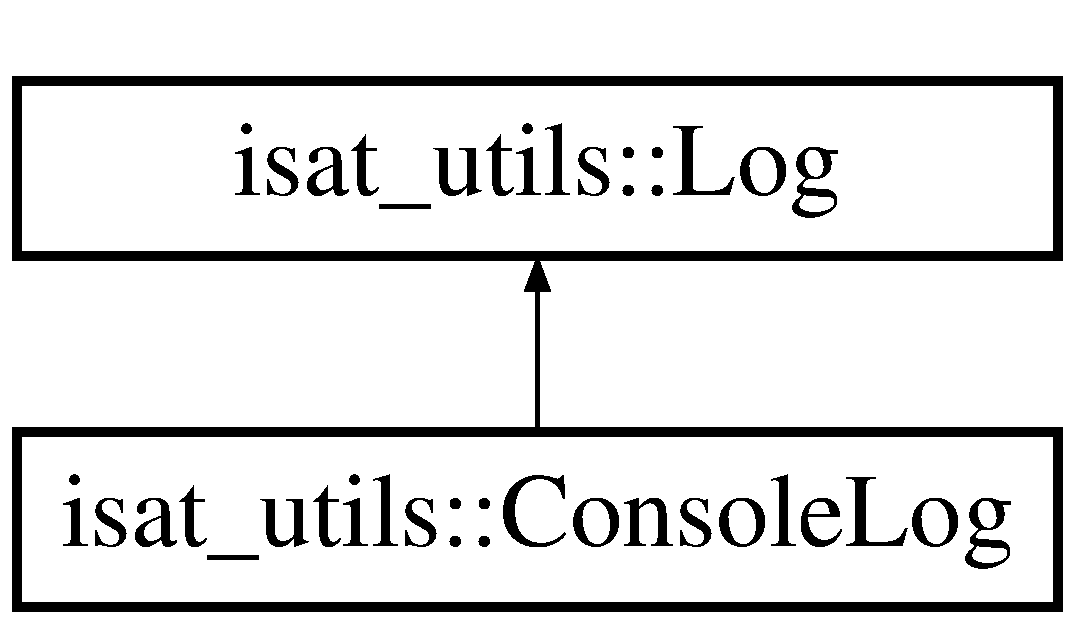
\includegraphics[height=2.000000cm]{classisat__utils_1_1_log}
\end{center}
\end{figure}
\subsection*{Public Member Functions}
\begin{DoxyCompactItemize}
\item 
virtual void {\bfseries set\+Log\+Filter} (\hyperlink{classisat__utils_1_1_log_filter}{Log\+Filter} $\ast$log\+Filter)\hypertarget{classisat__utils_1_1_log_aa14ecc43296c5642d40f52b840a469c1}{}\label{classisat__utils_1_1_log_aa14ecc43296c5642d40f52b840a469c1}

\item 
virtual \hyperlink{classisat__utils_1_1_log_filter}{Log\+Filter} $\ast$ {\bfseries get\+Log\+Filter} ()\hypertarget{classisat__utils_1_1_log_adba1fc3e5dd13337aa4a4ed29e965f48}{}\label{classisat__utils_1_1_log_adba1fc3e5dd13337aa4a4ed29e965f48}

\item 
virtual void {\bfseries set\+Log\+Formatter} (\hyperlink{classisat__utils_1_1_log_formatter}{Log\+Formatter} $\ast$log\+Formatter)\hypertarget{classisat__utils_1_1_log_aea0cc11c87f4d3fbd911391dd3757968}{}\label{classisat__utils_1_1_log_aea0cc11c87f4d3fbd911391dd3757968}

\item 
virtual \hyperlink{classisat__utils_1_1_log_formatter}{Log\+Formatter} $\ast$ {\bfseries get\+Log\+Formatter} ()\hypertarget{classisat__utils_1_1_log_a9ce01a492d2b707963f09afba58f9b9c}{}\label{classisat__utils_1_1_log_a9ce01a492d2b707963f09afba58f9b9c}

\item 
virtual bool {\bfseries write\+Entry} (Log\+Common\+::\+Log\+Level log\+Level, std\+::string logger\+Name, std\+::string message)\hypertarget{classisat__utils_1_1_log_a1d590f19a1f4f82b7709bb0d327096ba}{}\label{classisat__utils_1_1_log_a1d590f19a1f4f82b7709bb0d327096ba}

\end{DoxyCompactItemize}
\subsection*{Protected Attributes}
\begin{DoxyCompactItemize}
\item 
\hyperlink{classisat__utils_1_1_log_filter}{Log\+Filter} $\ast$ {\bfseries log\+Filter}\hypertarget{classisat__utils_1_1_log_acefd881551b3e427865154dbd280cded}{}\label{classisat__utils_1_1_log_acefd881551b3e427865154dbd280cded}

\item 
\hyperlink{classisat__utils_1_1_log_formatter}{Log\+Formatter} $\ast$ {\bfseries log\+Formatter}\hypertarget{classisat__utils_1_1_log_aa2faa91a1c9e3e86f96a912a2df7918c}{}\label{classisat__utils_1_1_log_aa2faa91a1c9e3e86f96a912a2df7918c}

\end{DoxyCompactItemize}


The documentation for this class was generated from the following files\+:\begin{DoxyCompactItemize}
\item 
/home/riley/work/fsw/src/isatgs/\+B\+A\+R\+Co\+Mm\+S/src/dependencies/utils/Log.\+h\item 
/home/riley/work/fsw/src/isatgs/\+B\+A\+R\+Co\+Mm\+S/src/dependencies/utils/Log.\+cpp\end{DoxyCompactItemize}

\hypertarget{classisat__utils_1_1_log_common}{}\section{isat\+\_\+utils\+:\+:Log\+Common Class Reference}
\label{classisat__utils_1_1_log_common}\index{isat\+\_\+utils\+::\+Log\+Common@{isat\+\_\+utils\+::\+Log\+Common}}
\subsection*{Public Types}
\begin{DoxyCompactItemize}
\item 
enum {\bfseries Log\+Level} \{ \\*
{\bfseries A\+LL} = 0, 
{\bfseries D\+E\+B\+UG} = 1, 
{\bfseries I\+N\+FO} = 2, 
{\bfseries W\+A\+RN} = 4, 
\\*
{\bfseries E\+R\+R\+OR} = 8, 
{\bfseries F\+A\+T\+AL} = 16, 
{\bfseries O\+FF} = 32
 \}\hypertarget{classisat__utils_1_1_log_common_a9fcc60e3eb21a64ea36a42a3084bb280}{}\label{classisat__utils_1_1_log_common_a9fcc60e3eb21a64ea36a42a3084bb280}

\end{DoxyCompactItemize}


The documentation for this class was generated from the following file\+:\begin{DoxyCompactItemize}
\item 
/home/riley/work/fsw/src/isatgs/\+B\+A\+R\+Co\+Mm\+S/src/dependencies/utils/Log\+Common.\+h\end{DoxyCompactItemize}

\hypertarget{classisat__utils_1_1_log_filter}{}\section{isat\+\_\+utils\+:\+:Log\+Filter Class Reference}
\label{classisat__utils_1_1_log_filter}\index{isat\+\_\+utils\+::\+Log\+Filter@{isat\+\_\+utils\+::\+Log\+Filter}}
Inheritance diagram for isat\+\_\+utils\+:\+:Log\+Filter\+:\begin{figure}[H]
\begin{center}
\leavevmode
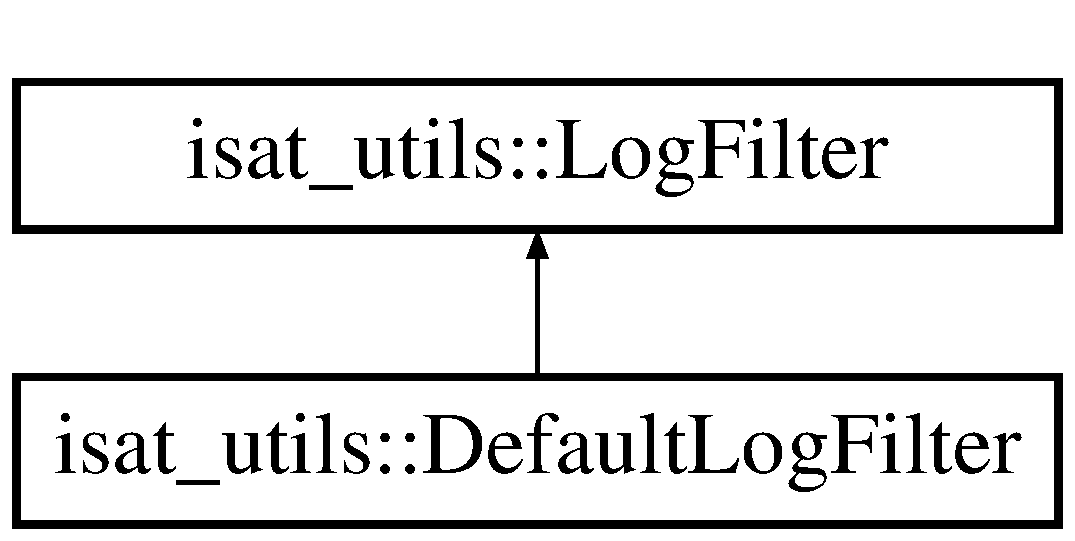
\includegraphics[height=2.000000cm]{classisat__utils_1_1_log_filter}
\end{center}
\end{figure}
\subsection*{Public Member Functions}
\begin{DoxyCompactItemize}
\item 
virtual bool {\bfseries check\+Entry} (Log\+Common\+::\+Log\+Level, std\+::string logger\+Name, std\+::string message)=0\hypertarget{classisat__utils_1_1_log_filter_a311a404daf5b6225f70352c06db02d2e}{}\label{classisat__utils_1_1_log_filter_a311a404daf5b6225f70352c06db02d2e}

\end{DoxyCompactItemize}


The documentation for this class was generated from the following file\+:\begin{DoxyCompactItemize}
\item 
/home/riley/work/fsw/src/isatgs/\+B\+A\+R\+Co\+Mm\+S/src/dependencies/utils/Log\+Filter.\+h\end{DoxyCompactItemize}

\hypertarget{classisat__utils_1_1_log_formatter}{}\section{isat\+\_\+utils\+:\+:Log\+Formatter Class Reference}
\label{classisat__utils_1_1_log_formatter}\index{isat\+\_\+utils\+::\+Log\+Formatter@{isat\+\_\+utils\+::\+Log\+Formatter}}
Inheritance diagram for isat\+\_\+utils\+:\+:Log\+Formatter\+:\begin{figure}[H]
\begin{center}
\leavevmode
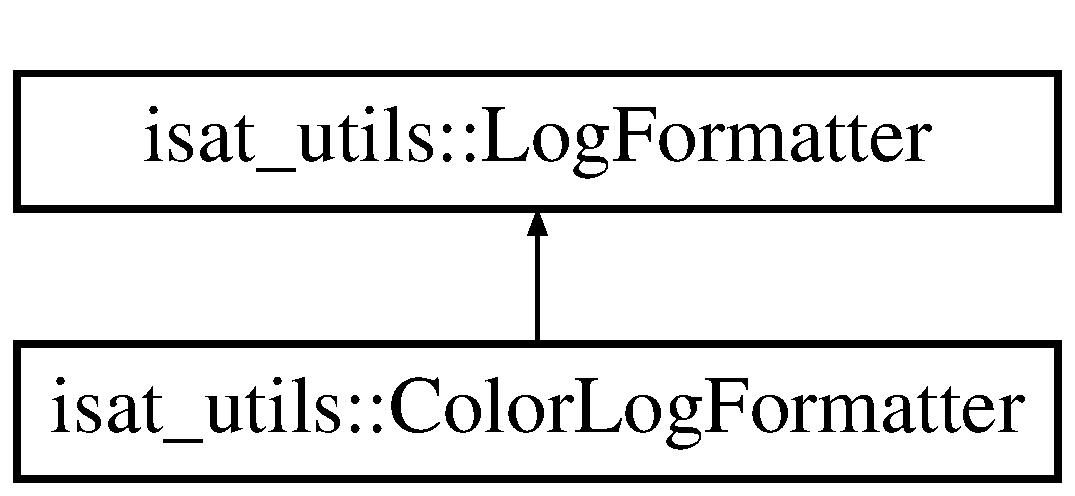
\includegraphics[height=2.000000cm]{classisat__utils_1_1_log_formatter}
\end{center}
\end{figure}
\subsection*{Public Member Functions}
\begin{DoxyCompactItemize}
\item 
virtual std\+::string {\bfseries get\+Log\+Entry} (time\+\_\+t entry\+Time, Log\+Common\+::\+Log\+Level log\+Level, std\+::string logger\+Name, std\+::string message)=0\hypertarget{classisat__utils_1_1_log_formatter_ae5dd8b0dc31ee35c6bd3b9c937e5106f}{}\label{classisat__utils_1_1_log_formatter_ae5dd8b0dc31ee35c6bd3b9c937e5106f}

\end{DoxyCompactItemize}


The documentation for this class was generated from the following file\+:\begin{DoxyCompactItemize}
\item 
/home/riley/work/fsw/src/isatgs/\+B\+A\+R\+Co\+Mm\+S/src/dependencies/utils/Log\+Formatter.\+h\end{DoxyCompactItemize}

\hypertarget{classisat__utils_1_1_logger}{}\section{isat\+\_\+utils\+:\+:Logger Class Reference}
\label{classisat__utils_1_1_logger}\index{isat\+\_\+utils\+::\+Logger@{isat\+\_\+utils\+::\+Logger}}
\subsection*{Public Member Functions}
\begin{DoxyCompactItemize}
\item 
{\bfseries Logger} (std\+::string logger\+Name)\hypertarget{classisat__utils_1_1_logger_a018ab14cec09fb2e9d69f730d14774f0}{}\label{classisat__utils_1_1_logger_a018ab14cec09fb2e9d69f730d14774f0}

\item 
void {\bfseries set\+Log} (\hyperlink{classisat__utils_1_1_log}{Log} $\ast$log)\hypertarget{classisat__utils_1_1_logger_acef3f6dec4c9206822b58e1ef8b5a802}{}\label{classisat__utils_1_1_logger_acef3f6dec4c9206822b58e1ef8b5a802}

\item 
void {\bfseries debug} (std\+::string message)\hypertarget{classisat__utils_1_1_logger_a5f343e722f2605b2d3af8528b66aeaae}{}\label{classisat__utils_1_1_logger_a5f343e722f2605b2d3af8528b66aeaae}

\item 
void {\bfseries info} (std\+::string message)\hypertarget{classisat__utils_1_1_logger_a603df91c9bac656280dd683619bbed35}{}\label{classisat__utils_1_1_logger_a603df91c9bac656280dd683619bbed35}

\item 
void {\bfseries warn} (std\+::string message)\hypertarget{classisat__utils_1_1_logger_a61d385a824293f2d05ec2389ed2b601d}{}\label{classisat__utils_1_1_logger_a61d385a824293f2d05ec2389ed2b601d}

\item 
void {\bfseries error} (std\+::string message)\hypertarget{classisat__utils_1_1_logger_acddaa197cc0643b43dcd62d5cda82b89}{}\label{classisat__utils_1_1_logger_acddaa197cc0643b43dcd62d5cda82b89}

\item 
void {\bfseries fatal} (std\+::string message)\hypertarget{classisat__utils_1_1_logger_ac279424c66b6f2b1d4d753f34a926c80}{}\label{classisat__utils_1_1_logger_ac279424c66b6f2b1d4d753f34a926c80}

\end{DoxyCompactItemize}
\subsection*{Protected Attributes}
\begin{DoxyCompactItemize}
\item 
std\+::string {\bfseries name}\hypertarget{classisat__utils_1_1_logger_aa8d63198108fbc1a1c350b089057e1bb}{}\label{classisat__utils_1_1_logger_aa8d63198108fbc1a1c350b089057e1bb}

\item 
\hyperlink{classisat__utils_1_1_log}{Log} $\ast$ {\bfseries log}\hypertarget{classisat__utils_1_1_logger_ad0ecb0d69ae02127dd00e26cea47016f}{}\label{classisat__utils_1_1_logger_ad0ecb0d69ae02127dd00e26cea47016f}

\end{DoxyCompactItemize}


The documentation for this class was generated from the following files\+:\begin{DoxyCompactItemize}
\item 
/home/riley/work/fsw/src/isatgs/\+B\+A\+R\+Co\+Mm\+S/src/dependencies/utils/Logger.\+h\item 
/home/riley/work/fsw/src/isatgs/\+B\+A\+R\+Co\+Mm\+S/src/dependencies/utils/Logger.\+cpp\end{DoxyCompactItemize}

\hypertarget{classisat__utils_1_1_log_manager}{}\section{isat\+\_\+utils\+:\+:Log\+Manager Class Reference}
\label{classisat__utils_1_1_log_manager}\index{isat\+\_\+utils\+::\+Log\+Manager@{isat\+\_\+utils\+::\+Log\+Manager}}
\subsection*{Public Member Functions}
\begin{DoxyCompactItemize}
\item 
bool {\bfseries add\+Log} (\hyperlink{classisat__utils_1_1_string}{String} log\+Name, \hyperlink{classisat__utils_1_1_log}{Log} $\ast$log)\hypertarget{classisat__utils_1_1_log_manager_aa7f5be31af219b7402229d21d283cc89}{}\label{classisat__utils_1_1_log_manager_aa7f5be31af219b7402229d21d283cc89}

\item 
\hyperlink{classisat__utils_1_1_log}{Log} $\ast$ {\bfseries get\+Default\+Log} ()\hypertarget{classisat__utils_1_1_log_manager_a9d723b5d0600a13fa13f5ce325bb522a}{}\label{classisat__utils_1_1_log_manager_a9d723b5d0600a13fa13f5ce325bb522a}

\item 
\hyperlink{classisat__utils_1_1_log}{Log} $\ast$ {\bfseries get\+Log} (\hyperlink{classisat__utils_1_1_string}{String} log\+Name)\hypertarget{classisat__utils_1_1_log_manager_a878a4eb7d28026d3dbae8cee2a118356}{}\label{classisat__utils_1_1_log_manager_a878a4eb7d28026d3dbae8cee2a118356}

\end{DoxyCompactItemize}
\subsection*{Static Public Member Functions}
\begin{DoxyCompactItemize}
\item 
static \hyperlink{classisat__utils_1_1_log_manager}{Log\+Manager} \& {\bfseries get\+Instance} ()\hypertarget{classisat__utils_1_1_log_manager_a66ce07ec98bb58794573ef324735cf8a}{}\label{classisat__utils_1_1_log_manager_a66ce07ec98bb58794573ef324735cf8a}

\end{DoxyCompactItemize}
\subsection*{Protected Attributes}
\begin{DoxyCompactItemize}
\item 
\hyperlink{classisat__utils_1_1_log}{Log} $\ast$ {\bfseries default\+Log}\hypertarget{classisat__utils_1_1_log_manager_a2bd75c3efdf4bffdf1e43465639a8a1c}{}\label{classisat__utils_1_1_log_manager_a2bd75c3efdf4bffdf1e43465639a8a1c}

\end{DoxyCompactItemize}


The documentation for this class was generated from the following files\+:\begin{DoxyCompactItemize}
\item 
/home/riley/work/fsw/src/isatgs/\+B\+A\+R\+Co\+Mm\+S/src/dependencies/utils/Log\+Manager.\+h\item 
/home/riley/work/fsw/src/isatgs/\+B\+A\+R\+Co\+Mm\+S/src/dependencies/utils/Log\+Manager.\+cpp\end{DoxyCompactItemize}

\hypertarget{struct_l_v}{}\section{LV Struct Reference}
\label{struct_l_v}\index{LV@{LV}}
\subsection*{Public Attributes}
\begin{DoxyCompactItemize}
\item 
u\+\_\+int\+\_\+1 {\bfseries length}\hypertarget{struct_l_v_aade78150507af2980eb6c8bb6b4321f4}{}\label{struct_l_v_aade78150507af2980eb6c8bb6b4321f4}

\item 
u\+\_\+int\+\_\+1 {\bfseries value} \mbox{[}M\+A\+X\+\_\+\+F\+I\+L\+E\+\_\+\+N\+A\+M\+E\+\_\+\+L\+E\+N\+G\+TH\mbox{]}\hypertarget{struct_l_v_a3e11374d15114b08bd518075a96ec39c}{}\label{struct_l_v_a3e11374d15114b08bd518075a96ec39c}

\end{DoxyCompactItemize}


The documentation for this struct was generated from the following file\+:\begin{DoxyCompactItemize}
\item 
/home/riley/work/fsw/src/isatgs/\+B\+A\+R\+Co\+Mm\+S/src/dependencies/\+C\+F\+D\+P/\+P\+R\+I/pdu.\+c\end{DoxyCompactItemize}

\hypertarget{struct_m_a_c_h_i_n_e}{}\section{M\+A\+C\+H\+I\+NE Struct Reference}
\label{struct_m_a_c_h_i_n_e}\index{M\+A\+C\+H\+I\+NE@{M\+A\+C\+H\+I\+NE}}
\subsection*{Public Attributes}
\begin{DoxyCompactItemize}
\item 
\hyperlink{struct_t_r_a_n_s___s_t_a_t_u_s}{T\+R\+A\+N\+S\+\_\+\+S\+T\+A\+T\+US} {\bfseries publik}\hypertarget{struct_m_a_c_h_i_n_e_a6c3d05a5a9281bec7b22605df99c08e8}{}\label{struct_m_a_c_h_i_n_e_a6c3d05a5a9281bec7b22605df99c08e8}

\item 
boolean {\bfseries has\+\_\+a\+\_\+pdu\+\_\+been\+\_\+received}\+:1\hypertarget{struct_m_a_c_h_i_n_e_ad4de08f39605e2f9e0ae9b842644397d}{}\label{struct_m_a_c_h_i_n_e_ad4de08f39605e2f9e0ae9b842644397d}

\item 
boolean {\bfseries has\+\_\+a\+\_\+put\+\_\+request\+\_\+been\+\_\+received}\+:1\hypertarget{struct_m_a_c_h_i_n_e_af6e7e6cd7219636d60aa319d214b02f1}{}\label{struct_m_a_c_h_i_n_e_af6e7e6cd7219636d60aa319d214b02f1}

\item 
boolean {\bfseries has\+\_\+eof\+\_\+been\+\_\+received}\+:1\hypertarget{struct_m_a_c_h_i_n_e_a791c795c9b8f94415bfef3e30f0cec42}{}\label{struct_m_a_c_h_i_n_e_a791c795c9b8f94415bfef3e30f0cec42}

\item 
boolean {\bfseries has\+\_\+eof\+\_\+been\+\_\+sent}\+:1\hypertarget{struct_m_a_c_h_i_n_e_ab4b8b566ffe5f9a843ed061f98803471}{}\label{struct_m_a_c_h_i_n_e_ab4b8b566ffe5f9a843ed061f98803471}

\item 
boolean {\bfseries has\+\_\+this\+\_\+state\+\_\+machine\+\_\+finished}\+:1\hypertarget{struct_m_a_c_h_i_n_e_a9f3d17df8d0b8d8c8051b9ad5f808a08}{}\label{struct_m_a_c_h_i_n_e_a9f3d17df8d0b8d8c8051b9ad5f808a08}

\item 
boolean {\bfseries have\+\_\+we\+\_\+initiated\+\_\+a\+\_\+cancel}\+:1\hypertarget{struct_m_a_c_h_i_n_e_a71b9a1432a405040140194f6bca1704a}{}\label{struct_m_a_c_h_i_n_e_a71b9a1432a405040140194f6bca1704a}

\item 
boolean {\bfseries is\+\_\+external\+\_\+xfer\+\_\+open}\+:1\hypertarget{struct_m_a_c_h_i_n_e_a80b275c61b5029c15b2121819bd7d201}{}\label{struct_m_a_c_h_i_n_e_a80b275c61b5029c15b2121819bd7d201}

\item 
boolean {\bfseries is\+\_\+outgoing\+\_\+ack\+\_\+buffered}\+:1\hypertarget{struct_m_a_c_h_i_n_e_aa343af0073ac10714f1a1dcf7c3fcca6}{}\label{struct_m_a_c_h_i_n_e_aa343af0073ac10714f1a1dcf7c3fcca6}

\item 
boolean {\bfseries is\+\_\+outgoing\+\_\+eof\+\_\+buffered}\+:1\hypertarget{struct_m_a_c_h_i_n_e_ab84ebd1e34a22baea85bb6dcab099cda}{}\label{struct_m_a_c_h_i_n_e_ab84ebd1e34a22baea85bb6dcab099cda}

\item 
boolean {\bfseries is\+\_\+outgoing\+\_\+fin\+\_\+buffered}\+:1\hypertarget{struct_m_a_c_h_i_n_e_ad62dd4df8bf3fd1f5aafdf5048ac3b4c}{}\label{struct_m_a_c_h_i_n_e_ad62dd4df8bf3fd1f5aafdf5048ac3b4c}

\item 
boolean {\bfseries is\+\_\+outgoing\+\_\+md\+\_\+buffered}\+:1\hypertarget{struct_m_a_c_h_i_n_e_a5d5f9c0653f11afdb99d7c34b6601b78}{}\label{struct_m_a_c_h_i_n_e_a5d5f9c0653f11afdb99d7c34b6601b78}

\item 
boolean {\bfseries is\+\_\+outgoing\+\_\+nak\+\_\+buffered}\+:1\hypertarget{struct_m_a_c_h_i_n_e_a315e01ff6a08b2cf084fdb6dc9e5f580}{}\label{struct_m_a_c_h_i_n_e_a315e01ff6a08b2cf084fdb6dc9e5f580}

\item 
boolean {\bfseries is\+\_\+there\+\_\+a\+\_\+temp\+\_\+file}\+:1\hypertarget{struct_m_a_c_h_i_n_e_a0a7025547a73c28e38adc39f04ad45f4}{}\label{struct_m_a_c_h_i_n_e_a0a7025547a73c28e38adc39f04ad45f4}

\item 
boolean {\bfseries is\+\_\+there\+\_\+an\+\_\+open\+\_\+file}\+:1\hypertarget{struct_m_a_c_h_i_n_e_a2a65fc5fc2a7f047af17d8b01cd28077}{}\label{struct_m_a_c_h_i_n_e_a2a65fc5fc2a7f047af17d8b01cd28077}

\item 
boolean {\bfseries is\+\_\+user\+\_\+inside\+\_\+the\+\_\+engine\+\_\+core}\+:1\hypertarget{struct_m_a_c_h_i_n_e_a0dee57b83bae5ff84bd25cb53cdeaa03}{}\label{struct_m_a_c_h_i_n_e_a0dee57b83bae5ff84bd25cb53cdeaa03}

\item 
boolean {\bfseries should\+\_\+external\+\_\+xfer\+\_\+be\+\_\+closed}\+:1\hypertarget{struct_m_a_c_h_i_n_e_a76935ecb4670a6b5d85f11437da9de5d}{}\label{struct_m_a_c_h_i_n_e_a76935ecb4670a6b5d85f11437da9de5d}

\item 
\hyperlink{struct_h_d_r}{H\+DR} {\bfseries hdr}\hypertarget{struct_m_a_c_h_i_n_e_abfab47e12f6dde6e337a40e626e69344}{}\label{struct_m_a_c_h_i_n_e_abfab47e12f6dde6e337a40e626e69344}

\item 
\hyperlink{struct_e_o_h_f}{E\+O\+HF} {\bfseries eof}\hypertarget{struct_m_a_c_h_i_n_e_a10896a7f7589f9a9d07fe736fc7dbfe9}{}\label{struct_m_a_c_h_i_n_e_a10896a7f7589f9a9d07fe736fc7dbfe9}

\item 
\hyperlink{struct_f_i_n}{F\+IN} {\bfseries fin}\hypertarget{struct_m_a_c_h_i_n_e_a53699b59fdc5c35fd9c65b9be8595891}{}\label{struct_m_a_c_h_i_n_e_a53699b59fdc5c35fd9c65b9be8595891}

\item 
\hyperlink{struct_a_c_k}{A\+CK} {\bfseries ack}\hypertarget{struct_m_a_c_h_i_n_e_aeb46efb7b2b8a9ba78cae575666fe5ba}{}\label{struct_m_a_c_h_i_n_e_aeb46efb7b2b8a9ba78cae575666fe5ba}

\item 
\hyperlink{struct_n_a_k}{N\+AK} {\bfseries nak}\hypertarget{struct_m_a_c_h_i_n_e_a1f554312ebb28922a00c92a194cdfbcc}{}\label{struct_m_a_c_h_i_n_e_a1f554312ebb28922a00c92a194cdfbcc}

\item 
\hyperlink{struct_t_i_m_e_r}{T\+I\+M\+ER} {\bfseries ack\+\_\+timer}\hypertarget{struct_m_a_c_h_i_n_e_a2becfb37bd030c6c5831f73f17f59096}{}\label{struct_m_a_c_h_i_n_e_a2becfb37bd030c6c5831f73f17f59096}

\item 
\hyperlink{struct_t_i_m_e_r}{T\+I\+M\+ER} {\bfseries inactivity\+\_\+timer}\hypertarget{struct_m_a_c_h_i_n_e_aa90e121947901483be899bd6a160d577}{}\label{struct_m_a_c_h_i_n_e_aa90e121947901483be899bd6a160d577}

\item 
\hyperlink{struct_t_i_m_e_r}{T\+I\+M\+ER} {\bfseries nak\+\_\+timer}\hypertarget{struct_m_a_c_h_i_n_e_a71d4fea80d390eeb5aa124caca9f006b}{}\label{struct_m_a_c_h_i_n_e_a71d4fea80d390eeb5aa124caca9f006b}

\item 
F\+I\+LE $\ast$ {\bfseries fp}\hypertarget{struct_m_a_c_h_i_n_e_a0892fd0c53969ae7acdf590bc2e4a2be}{}\label{struct_m_a_c_h_i_n_e_a0892fd0c53969ae7acdf590bc2e4a2be}

\end{DoxyCompactItemize}


The documentation for this struct was generated from the following file\+:\begin{DoxyCompactItemize}
\item 
/home/riley/work/fsw/src/isatgs/\+B\+A\+R\+Co\+Mm\+S/src/dependencies/\+C\+F\+D\+P/\+P\+R\+I/machine.\+h\end{DoxyCompactItemize}

\hypertarget{struct_m_d}{}\section{MD Struct Reference}
\label{struct_m_d}\index{MD@{MD}}
\subsection*{Public Attributes}
\begin{DoxyCompactItemize}
\item 
boolean {\bfseries file\+\_\+transfer}\+: 1\hypertarget{struct_m_d_af43b09440cf76cde397e8d876c3a8130}{}\label{struct_m_d_af43b09440cf76cde397e8d876c3a8130}

\item 
boolean {\bfseries segmentation\+\_\+control}\+: 1\hypertarget{struct_m_d_a8483756b650d370a9f73c5eb67d5a981}{}\label{struct_m_d_a8483756b650d370a9f73c5eb67d5a981}

\item 
u\+\_\+int\+\_\+4 {\bfseries file\+\_\+size}\hypertarget{struct_m_d_ab0d079723734fa10ae2e95e81e63f128}{}\label{struct_m_d_ab0d079723734fa10ae2e95e81e63f128}

\item 
char {\bfseries source\+\_\+file\+\_\+name} \mbox{[}M\+A\+X\+\_\+\+F\+I\+L\+E\+\_\+\+N\+A\+M\+E\+\_\+\+L\+E\+N\+G\+TH+1\mbox{]}\hypertarget{struct_m_d_aeb82449d4978e44cd985a0f9be799396}{}\label{struct_m_d_aeb82449d4978e44cd985a0f9be799396}

\item 
char {\bfseries dest\+\_\+file\+\_\+name} \mbox{[}M\+A\+X\+\_\+\+F\+I\+L\+E\+\_\+\+N\+A\+M\+E\+\_\+\+L\+E\+N\+G\+TH+1\mbox{]}\hypertarget{struct_m_d_a5a85cb4df082239b96234b800e174870}{}\label{struct_m_d_a5a85cb4df082239b96234b800e174870}

\end{DoxyCompactItemize}


The documentation for this struct was generated from the following file\+:\begin{DoxyCompactItemize}
\item 
/home/riley/work/fsw/src/isatgs/\+B\+A\+R\+Co\+Mm\+S/src/dependencies/\+C\+F\+D\+P/\+P\+U\+B/cfdp\+\_\+data\+\_\+structures.\+h\end{DoxyCompactItemize}

\hypertarget{classtinyxml2_1_1_mem_pool}{}\section{tinyxml2\+:\+:Mem\+Pool Class Reference}
\label{classtinyxml2_1_1_mem_pool}\index{tinyxml2\+::\+Mem\+Pool@{tinyxml2\+::\+Mem\+Pool}}
Inheritance diagram for tinyxml2\+:\+:Mem\+Pool\+:\begin{figure}[H]
\begin{center}
\leavevmode
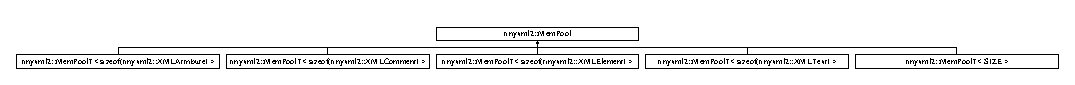
\includegraphics[height=0.691358cm]{classtinyxml2_1_1_mem_pool}
\end{center}
\end{figure}
\subsection*{Public Member Functions}
\begin{DoxyCompactItemize}
\item 
virtual int {\bfseries Item\+Size} () const  =0\hypertarget{classtinyxml2_1_1_mem_pool_afb3d8c6cbe91b44f90043d0d94dc7306}{}\label{classtinyxml2_1_1_mem_pool_afb3d8c6cbe91b44f90043d0d94dc7306}

\item 
virtual void $\ast$ {\bfseries Alloc} ()=0\hypertarget{classtinyxml2_1_1_mem_pool_a4f977b5fed752c0bbfe5295f469d6449}{}\label{classtinyxml2_1_1_mem_pool_a4f977b5fed752c0bbfe5295f469d6449}

\item 
virtual void {\bfseries Free} (void $\ast$)=0\hypertarget{classtinyxml2_1_1_mem_pool_a49e3bfac2cba2ebd6776b31e571f64f7}{}\label{classtinyxml2_1_1_mem_pool_a49e3bfac2cba2ebd6776b31e571f64f7}

\item 
virtual void {\bfseries Set\+Tracked} ()=0\hypertarget{classtinyxml2_1_1_mem_pool_ac5804dd1387b2e4de5eef710076a0db1}{}\label{classtinyxml2_1_1_mem_pool_ac5804dd1387b2e4de5eef710076a0db1}

\end{DoxyCompactItemize}


The documentation for this class was generated from the following file\+:\begin{DoxyCompactItemize}
\item 
/home/riley/work/fsw/src/isatgs/\+B\+A\+R\+Co\+Mm\+S/src/dependencies/utils/tinyxml2.\+h\end{DoxyCompactItemize}

\hypertarget{classtinyxml2_1_1_mem_pool_t}{}\section{tinyxml2\+:\+:Mem\+PoolT$<$ S\+I\+ZE $>$ Class Template Reference}
\label{classtinyxml2_1_1_mem_pool_t}\index{tinyxml2\+::\+Mem\+Pool\+T$<$ S\+I\+Z\+E $>$@{tinyxml2\+::\+Mem\+Pool\+T$<$ S\+I\+Z\+E $>$}}
Inheritance diagram for tinyxml2\+:\+:Mem\+PoolT$<$ S\+I\+ZE $>$\+:\begin{figure}[H]
\begin{center}
\leavevmode
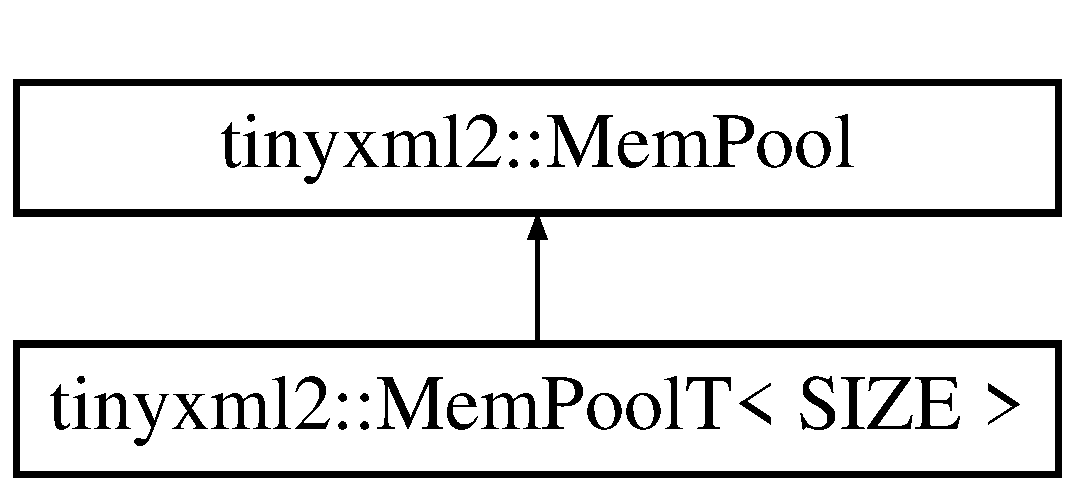
\includegraphics[height=2.000000cm]{classtinyxml2_1_1_mem_pool_t}
\end{center}
\end{figure}
\subsection*{Public Types}
\begin{DoxyCompactItemize}
\item 
enum \{ {\bfseries C\+O\+U\+NT} = (4$\ast$1024)/\+S\+I\+ZE
 \}\hypertarget{classtinyxml2_1_1_mem_pool_t_af9de1b2544c6553c3f8a75dd75c2f8f5}{}\label{classtinyxml2_1_1_mem_pool_t_af9de1b2544c6553c3f8a75dd75c2f8f5}

\end{DoxyCompactItemize}
\subsection*{Public Member Functions}
\begin{DoxyCompactItemize}
\item 
virtual int {\bfseries Item\+Size} () const \hypertarget{classtinyxml2_1_1_mem_pool_t_a7ec8778fe99f6e332615a703be0b48bc}{}\label{classtinyxml2_1_1_mem_pool_t_a7ec8778fe99f6e332615a703be0b48bc}

\item 
int {\bfseries Current\+Allocs} () const \hypertarget{classtinyxml2_1_1_mem_pool_t_a56be11b7db6a7ef00db17088a7769aab}{}\label{classtinyxml2_1_1_mem_pool_t_a56be11b7db6a7ef00db17088a7769aab}

\item 
virtual void $\ast$ {\bfseries Alloc} ()\hypertarget{classtinyxml2_1_1_mem_pool_t_aa9d785a48ffe6ea1be679bab13464486}{}\label{classtinyxml2_1_1_mem_pool_t_aa9d785a48ffe6ea1be679bab13464486}

\item 
virtual void {\bfseries Free} (void $\ast$mem)\hypertarget{classtinyxml2_1_1_mem_pool_t_a4f1a0c434e9e3d7391e5c16ed4ee8c70}{}\label{classtinyxml2_1_1_mem_pool_t_a4f1a0c434e9e3d7391e5c16ed4ee8c70}

\item 
void {\bfseries Trace} (const char $\ast$name)\hypertarget{classtinyxml2_1_1_mem_pool_t_a0bc596f271e0f139822c534238b3f244}{}\label{classtinyxml2_1_1_mem_pool_t_a0bc596f271e0f139822c534238b3f244}

\item 
void {\bfseries Set\+Tracked} ()\hypertarget{classtinyxml2_1_1_mem_pool_t_a7798932414916199a1bc0f9c3f368521}{}\label{classtinyxml2_1_1_mem_pool_t_a7798932414916199a1bc0f9c3f368521}

\item 
int {\bfseries Untracked} () const \hypertarget{classtinyxml2_1_1_mem_pool_t_a524b90d0edeac41964c06510757dce0f}{}\label{classtinyxml2_1_1_mem_pool_t_a524b90d0edeac41964c06510757dce0f}

\end{DoxyCompactItemize}


The documentation for this class was generated from the following file\+:\begin{DoxyCompactItemize}
\item 
/home/riley/work/fsw/src/isatgs/\+B\+A\+R\+Co\+Mm\+S/src/dependencies/utils/tinyxml2.\+h\end{DoxyCompactItemize}

\hypertarget{struct_message_classes}{}\section{Message\+Classes Struct Reference}
\label{struct_message_classes}\index{Message\+Classes@{Message\+Classes}}
\subsection*{Public Attributes}
\begin{DoxyCompactItemize}
\item 
bool {\bfseries all}\hypertarget{struct_message_classes_a459558add80cc299ef30b600678a6a9c}{}\label{struct_message_classes_a459558add80cc299ef30b600678a6a9c}

\item 
bool {\bfseries indications}\hypertarget{struct_message_classes_ada72923f89c3907adb6f37779b661cd3}{}\label{struct_message_classes_ada72923f89c3907adb6f37779b661cd3}

\item 
bool {\bfseries debug\+Memory\+Use}\hypertarget{struct_message_classes_a19e0d88e17d1024dc460f805506d645d}{}\label{struct_message_classes_a19e0d88e17d1024dc460f805506d645d}

\item 
bool {\bfseries debug\+N\+AK}\hypertarget{struct_message_classes_a5b2f5a45eb2479cb9a28d303b67a1ca8}{}\label{struct_message_classes_a5b2f5a45eb2479cb9a28d303b67a1ca8}

\item 
bool {\bfseries debug\+P\+DU}\hypertarget{struct_message_classes_ad0788d080ecf37d92e7a208f4b609111}{}\label{struct_message_classes_ad0788d080ecf37d92e7a208f4b609111}

\item 
bool {\bfseries P\+D\+U\+Filedata}\hypertarget{struct_message_classes_a07f8452b10aa59778bef0d495ab8214e}{}\label{struct_message_classes_a07f8452b10aa59778bef0d495ab8214e}

\item 
bool {\bfseries P\+D\+U\+Non\+Filedata}\hypertarget{struct_message_classes_ad25fad59c0711cadb187c2333790a385}{}\label{struct_message_classes_ad25fad59c0711cadb187c2333790a385}

\item 
bool {\bfseries P\+D\+U\+Retransmitted\+FD}\hypertarget{struct_message_classes_ad4c2d314b335b141c8f3d89e9f359b3c}{}\label{struct_message_classes_ad4c2d314b335b141c8f3d89e9f359b3c}

\item 
bool {\bfseries state\+All}\hypertarget{struct_message_classes_a666f3e3f94abc6353ea695b860c1c64f}{}\label{struct_message_classes_a666f3e3f94abc6353ea695b860c1c64f}

\item 
bool {\bfseries state\+Change}\hypertarget{struct_message_classes_ae9310b35d91d21bf82b049817028a569}{}\label{struct_message_classes_ae9310b35d91d21bf82b049817028a569}

\end{DoxyCompactItemize}


The documentation for this struct was generated from the following file\+:\begin{DoxyCompactItemize}
\item 
/home/riley/work/fsw/src/isatgs/\+B\+A\+R\+Co\+Mm\+S/src/modules/\+B\+A\+R\+Co\+Mm\+S\+\_\+\+C\+F\+D\+P/cfdpstructs.\+h\end{DoxyCompactItemize}

\hypertarget{struct_m_i_b}{}\section{M\+IB Struct Reference}
\label{struct_m_i_b}\index{M\+IB@{M\+IB}}
\subsection*{Public Attributes}
\begin{DoxyCompactItemize}
\item 
char {\bfseries E\+O\+F\+Recv} \mbox{[}C\+H\+O\+I\+C\+E\+\_\+\+S\+I\+ZE\mbox{]}\hypertarget{struct_m_i_b_a78814c0b7ecef3676e8cc31962f81e0b}{}\label{struct_m_i_b_a78814c0b7ecef3676e8cc31962f81e0b}

\item 
char {\bfseries E\+O\+F\+Sent} \mbox{[}C\+H\+O\+I\+C\+E\+\_\+\+S\+I\+ZE\mbox{]}\hypertarget{struct_m_i_b_a870b9fd10712b93d5e445bae372aeb6f}{}\label{struct_m_i_b_a870b9fd10712b93d5e445bae372aeb6f}

\item 
char {\bfseries file\+Recv} \mbox{[}C\+H\+O\+I\+C\+E\+\_\+\+S\+I\+ZE\mbox{]}\hypertarget{struct_m_i_b_a42bfa6c33713954f66c1829c59ff418f}{}\label{struct_m_i_b_a42bfa6c33713954f66c1829c59ff418f}

\item 
char {\bfseries file\+Sent} \mbox{[}C\+H\+O\+I\+C\+E\+\_\+\+S\+I\+ZE\mbox{]}\hypertarget{struct_m_i_b_a2a17c52b8eee5a9176edf4e8bdc240d6}{}\label{struct_m_i_b_a2a17c52b8eee5a9176edf4e8bdc240d6}

\item 
char {\bfseries ID} \mbox{[}N\+O\+D\+E\+\_\+\+S\+I\+ZE\mbox{]}\hypertarget{struct_m_i_b_aaade5496d0fdd3cb41c6fca9631e07dc}{}\label{struct_m_i_b_aaade5496d0fdd3cb41c6fca9631e07dc}

\item 
char {\bfseries resumed} \mbox{[}C\+H\+O\+I\+C\+E\+\_\+\+S\+I\+ZE\mbox{]}\hypertarget{struct_m_i_b_ae3f75a16b80dd605f6ae71d6ffb0e17c}{}\label{struct_m_i_b_ae3f75a16b80dd605f6ae71d6ffb0e17c}

\item 
char {\bfseries save} \mbox{[}C\+H\+O\+I\+C\+E\+\_\+\+S\+I\+ZE\mbox{]}\hypertarget{struct_m_i_b_a7c1a3686c6f4bb3c1a81d8c4091257e2}{}\label{struct_m_i_b_a7c1a3686c6f4bb3c1a81d8c4091257e2}

\item 
char {\bfseries suspended} \mbox{[}C\+H\+O\+I\+C\+E\+\_\+\+S\+I\+ZE\mbox{]}\hypertarget{struct_m_i_b_a9bd11b3b0c7aa8c09efcc921282afd37}{}\label{struct_m_i_b_a9bd11b3b0c7aa8c09efcc921282afd37}

\item 
char {\bfseries trans\+Fin} \mbox{[}C\+H\+O\+I\+C\+E\+\_\+\+S\+I\+ZE\mbox{]}\hypertarget{struct_m_i_b_a5c9ded36f5b0cbb804de34459e2b6b2b}{}\label{struct_m_i_b_a5c9ded36f5b0cbb804de34459e2b6b2b}

\item 
unsigned int {\bfseries A\+C\+K\+Limit}\hypertarget{struct_m_i_b_a1c05578ed1122584ec51b7174a25bbf5}{}\label{struct_m_i_b_a1c05578ed1122584ec51b7174a25bbf5}

\item 
unsigned int {\bfseries A\+C\+K\+Timeout}\hypertarget{struct_m_i_b_a5def7362f799cdd5727896fa8f61863b}{}\label{struct_m_i_b_a5def7362f799cdd5727896fa8f61863b}

\item 
unsigned int {\bfseries chunk\+Size}\hypertarget{struct_m_i_b_a01015d449aaabad31048f69b0796c9d7}{}\label{struct_m_i_b_a01015d449aaabad31048f69b0796c9d7}

\item 
unsigned int {\bfseries inactivity}\hypertarget{struct_m_i_b_ad21ba2f674f99bb3955576471def1dff}{}\label{struct_m_i_b_ad21ba2f674f99bb3955576471def1dff}

\item 
unsigned int {\bfseries N\+A\+K\+Limit}\hypertarget{struct_m_i_b_adab59c56faca2ea5db7aaa3855beb701}{}\label{struct_m_i_b_adab59c56faca2ea5db7aaa3855beb701}

\item 
unsigned int {\bfseries N\+A\+K\+Timeout}\hypertarget{struct_m_i_b_a7c95cca4afcb24856aafa70a3fb6ef81}{}\label{struct_m_i_b_a7c95cca4afcb24856aafa70a3fb6ef81}

\end{DoxyCompactItemize}


The documentation for this struct was generated from the following file\+:\begin{DoxyCompactItemize}
\item 
/home/riley/work/fsw/src/isatgs/\+B\+A\+R\+Co\+Mm\+S/src/modules/\+B\+A\+R\+Co\+Mm\+S\+\_\+\+C\+F\+D\+P/cfdpstructs.\+h\end{DoxyCompactItemize}

\hypertarget{struct_m_i_b___l_o_c_a_l}{}\section{M\+I\+B\+\_\+\+L\+O\+C\+AL Struct Reference}
\label{struct_m_i_b___l_o_c_a_l}\index{M\+I\+B\+\_\+\+L\+O\+C\+AL@{M\+I\+B\+\_\+\+L\+O\+C\+AL}}
\subsection*{Public Attributes}
\begin{DoxyCompactItemize}
\item 
boolean {\bfseries issue\+\_\+eof\+\_\+recv}\hypertarget{struct_m_i_b___l_o_c_a_l_a772be7fb8b1c5840d6b22dc59e948806}{}\label{struct_m_i_b___l_o_c_a_l_a772be7fb8b1c5840d6b22dc59e948806}

\item 
boolean {\bfseries issue\+\_\+eof\+\_\+sent}\hypertarget{struct_m_i_b___l_o_c_a_l_a3d9596a8697dee9e15c8d006e929cf11}{}\label{struct_m_i_b___l_o_c_a_l_a3d9596a8697dee9e15c8d006e929cf11}

\item 
boolean {\bfseries issue\+\_\+file\+\_\+segment\+\_\+recv}\hypertarget{struct_m_i_b___l_o_c_a_l_a546d00e23de68e7bbfc8dddd934bed25}{}\label{struct_m_i_b___l_o_c_a_l_a546d00e23de68e7bbfc8dddd934bed25}

\item 
boolean {\bfseries issue\+\_\+file\+\_\+segment\+\_\+sent}\hypertarget{struct_m_i_b___l_o_c_a_l_a86ddf6121969386d1bc4eac6ee8bd49c}{}\label{struct_m_i_b___l_o_c_a_l_a86ddf6121969386d1bc4eac6ee8bd49c}

\item 
boolean {\bfseries issue\+\_\+resumed}\hypertarget{struct_m_i_b___l_o_c_a_l_a574f5afa306f24ee4b018a597837a8c0}{}\label{struct_m_i_b___l_o_c_a_l_a574f5afa306f24ee4b018a597837a8c0}

\item 
boolean {\bfseries issue\+\_\+suspended}\hypertarget{struct_m_i_b___l_o_c_a_l_abbc94e7d82c735a48a614eb5ee673a88}{}\label{struct_m_i_b___l_o_c_a_l_abbc94e7d82c735a48a614eb5ee673a88}

\item 
boolean {\bfseries issue\+\_\+transaction\+\_\+finished}\hypertarget{struct_m_i_b___l_o_c_a_l_a4011dd5b6a49f6d472dd91c51d8f8668}{}\label{struct_m_i_b___l_o_c_a_l_a4011dd5b6a49f6d472dd91c51d8f8668}

\item 
\hyperlink{struct_i_d}{ID} {\bfseries my\+\_\+id}\hypertarget{struct_m_i_b___l_o_c_a_l_a42577e4d333d9c521f21fe923adc789c}{}\label{struct_m_i_b___l_o_c_a_l_a42577e4d333d9c521f21fe923adc789c}

\item 
u\+\_\+int\+\_\+1 {\bfseries response} \mbox{[}N\+U\+M\+B\+E\+R\+\_\+\+O\+F\+\_\+\+C\+O\+N\+D\+I\+T\+I\+O\+N\+\_\+\+C\+O\+D\+ES\mbox{]}\hypertarget{struct_m_i_b___l_o_c_a_l_a5825a2886e9cf25547b07e49bbccc98b}{}\label{struct_m_i_b___l_o_c_a_l_a5825a2886e9cf25547b07e49bbccc98b}

\end{DoxyCompactItemize}


The documentation for this struct was generated from the following file\+:\begin{DoxyCompactItemize}
\item 
/home/riley/work/fsw/src/isatgs/\+B\+A\+R\+Co\+Mm\+S/src/dependencies/\+C\+F\+D\+P/\+P\+R\+I/mib.\+c\end{DoxyCompactItemize}

\hypertarget{struct_m_i_b___r_e_m_o_t_e}{}\section{M\+I\+B\+\_\+\+R\+E\+M\+O\+TE Struct Reference}
\label{struct_m_i_b___r_e_m_o_t_e}\index{M\+I\+B\+\_\+\+R\+E\+M\+O\+TE@{M\+I\+B\+\_\+\+R\+E\+M\+O\+TE}}
\subsection*{Public Attributes}
\begin{DoxyCompactItemize}
\item 
u\+\_\+int\+\_\+4 {\bfseries ack\+\_\+limit}\hypertarget{struct_m_i_b___r_e_m_o_t_e_ab916fe8e94e822dbf35ad96e39e34814}{}\label{struct_m_i_b___r_e_m_o_t_e_ab916fe8e94e822dbf35ad96e39e34814}

\item 
u\+\_\+int\+\_\+4 {\bfseries ack\+\_\+timeout}\hypertarget{struct_m_i_b___r_e_m_o_t_e_a83cd675ea83beabf777aabdb839c5077}{}\label{struct_m_i_b___r_e_m_o_t_e_a83cd675ea83beabf777aabdb839c5077}

\item 
u\+\_\+int\+\_\+4 {\bfseries inactivity\+\_\+timeout}\hypertarget{struct_m_i_b___r_e_m_o_t_e_a4ec02fe58abf86cd3d9c20e922161445}{}\label{struct_m_i_b___r_e_m_o_t_e_a4ec02fe58abf86cd3d9c20e922161445}

\item 
u\+\_\+int\+\_\+4 {\bfseries nak\+\_\+limit}\hypertarget{struct_m_i_b___r_e_m_o_t_e_a1436d945c1948dadbc8a2cb261028466}{}\label{struct_m_i_b___r_e_m_o_t_e_a1436d945c1948dadbc8a2cb261028466}

\item 
u\+\_\+int\+\_\+4 {\bfseries nak\+\_\+timeout}\hypertarget{struct_m_i_b___r_e_m_o_t_e_a7484587bfb6f523e69dd66bd52dec16e}{}\label{struct_m_i_b___r_e_m_o_t_e_a7484587bfb6f523e69dd66bd52dec16e}

\item 
u\+\_\+int\+\_\+4 {\bfseries outgoing\+\_\+file\+\_\+chunk\+\_\+size}\hypertarget{struct_m_i_b___r_e_m_o_t_e_af30900d9c5edd454a7d604dd648c9949}{}\label{struct_m_i_b___r_e_m_o_t_e_af30900d9c5edd454a7d604dd648c9949}

\item 
boolean {\bfseries save\+\_\+incomplete\+\_\+files}\hypertarget{struct_m_i_b___r_e_m_o_t_e_a34f829c726d85f79f761308d32f97aa4}{}\label{struct_m_i_b___r_e_m_o_t_e_a34f829c726d85f79f761308d32f97aa4}

\end{DoxyCompactItemize}


The documentation for this struct was generated from the following file\+:\begin{DoxyCompactItemize}
\item 
/home/riley/work/fsw/src/isatgs/\+B\+A\+R\+Co\+Mm\+S/src/dependencies/\+C\+F\+D\+P/\+P\+R\+I/mib.\+c\end{DoxyCompactItemize}

\hypertarget{struct_n_a_k}{}\section{N\+AK Struct Reference}
\label{struct_n_a_k}\index{N\+AK@{N\+AK}}
\subsection*{Public Attributes}
\begin{DoxyCompactItemize}
\item 
u\+\_\+int\+\_\+4 {\bfseries start\+\_\+of\+\_\+scope}\hypertarget{struct_n_a_k_aee9506694f57879a52b982775a89a447}{}\label{struct_n_a_k_aee9506694f57879a52b982775a89a447}

\item 
u\+\_\+int\+\_\+4 {\bfseries end\+\_\+of\+\_\+scope}\hypertarget{struct_n_a_k_a046120aa9a95115f4bb0b5a66a6dbdff}{}\label{struct_n_a_k_a046120aa9a95115f4bb0b5a66a6dbdff}

\item 
boolean {\bfseries is\+\_\+metadata\+\_\+missing}\+: 1\hypertarget{struct_n_a_k_a10a9c51ea5f393093f2814362cc9d939}{}\label{struct_n_a_k_a10a9c51ea5f393093f2814362cc9d939}

\item 
\hyperlink{structgap}{G\+AP} $\ast$ {\bfseries head}\hypertarget{struct_n_a_k_abc8812e8a65c2078604e01f676830569}{}\label{struct_n_a_k_abc8812e8a65c2078604e01f676830569}

\item 
boolean {\bfseries in\+\_\+use} \mbox{[}M\+A\+X\+\_\+\+G\+A\+P\+S\+\_\+\+P\+E\+R\+\_\+\+T\+R\+A\+N\+S\+A\+C\+T\+I\+ON\mbox{]}\hypertarget{struct_n_a_k_a2ae41f6899529ee96e3339d4cbce8c4a}{}\label{struct_n_a_k_a2ae41f6899529ee96e3339d4cbce8c4a}

\item 
\hyperlink{structgap}{G\+AP} {\bfseries gap} \mbox{[}M\+A\+X\+\_\+\+G\+A\+P\+S\+\_\+\+P\+E\+R\+\_\+\+T\+R\+A\+N\+S\+A\+C\+T\+I\+ON\mbox{]}\hypertarget{struct_n_a_k_af1e1ca6e491d5e9b343e8e30d2c9e112}{}\label{struct_n_a_k_af1e1ca6e491d5e9b343e8e30d2c9e112}

\end{DoxyCompactItemize}


The documentation for this struct was generated from the following file\+:\begin{DoxyCompactItemize}
\item 
/home/riley/work/fsw/src/isatgs/\+B\+A\+R\+Co\+Mm\+S/src/dependencies/\+C\+F\+D\+P/\+P\+R\+I/structures.\+h\end{DoxyCompactItemize}

\hypertarget{struct_n_o_d_e___c_o_m_m}{}\section{N\+O\+D\+E\+\_\+\+C\+O\+MM Struct Reference}
\label{struct_n_o_d_e___c_o_m_m}\index{N\+O\+D\+E\+\_\+\+C\+O\+MM@{N\+O\+D\+E\+\_\+\+C\+O\+MM}}
\subsection*{Public Attributes}
\begin{DoxyCompactItemize}
\item 
C\+O\+M\+M\+\_\+\+T\+Y\+PE {\bfseries type}\hypertarget{struct_n_o_d_e___c_o_m_m_ae294165d1e79a7915f8cdae0d7e8bbff}{}\label{struct_n_o_d_e___c_o_m_m_ae294165d1e79a7915f8cdae0d7e8bbff}

\item 
\begin{tabbing}
xx\=xx\=xx\=xx\=xx\=xx\=xx\=xx\=xx\=\kill
union \{\\
\>\hyperlink{struct_u_d_p___p_a_r_a_m_e_t_e_r_s}{UDP\_PARAMETERS} {\bfseries udp}\\
\} {\bfseries parameters}\hypertarget{struct_n_o_d_e___c_o_m_m_ae8384f18a81031b64f98fdb5f37e8f55}{}\label{struct_n_o_d_e___c_o_m_m_ae8384f18a81031b64f98fdb5f37e8f55}
\\

\end{tabbing}\end{DoxyCompactItemize}


The documentation for this struct was generated from the following file\+:\begin{DoxyCompactItemize}
\item 
/home/riley/work/fsw/src/isatgs/\+B\+A\+R\+Co\+Mm\+S/src/dependencies/\+C\+F\+D\+P/\+C\+O\+D\+E/comm.\+c\end{DoxyCompactItemize}

\hypertarget{classisat__trek_1_1_oper_mode___command}{}\section{isat\+\_\+trek\+:\+:Oper\+Mode\+\_\+\+Command Class Reference}
\label{classisat__trek_1_1_oper_mode___command}\index{isat\+\_\+trek\+::\+Oper\+Mode\+\_\+\+Command@{isat\+\_\+trek\+::\+Oper\+Mode\+\_\+\+Command}}


{\ttfamily \#include $<$Oper\+Mode\+\_\+\+Command.\+h$>$}

Inheritance diagram for isat\+\_\+trek\+:\+:Oper\+Mode\+\_\+\+Command\+:\begin{figure}[H]
\begin{center}
\leavevmode
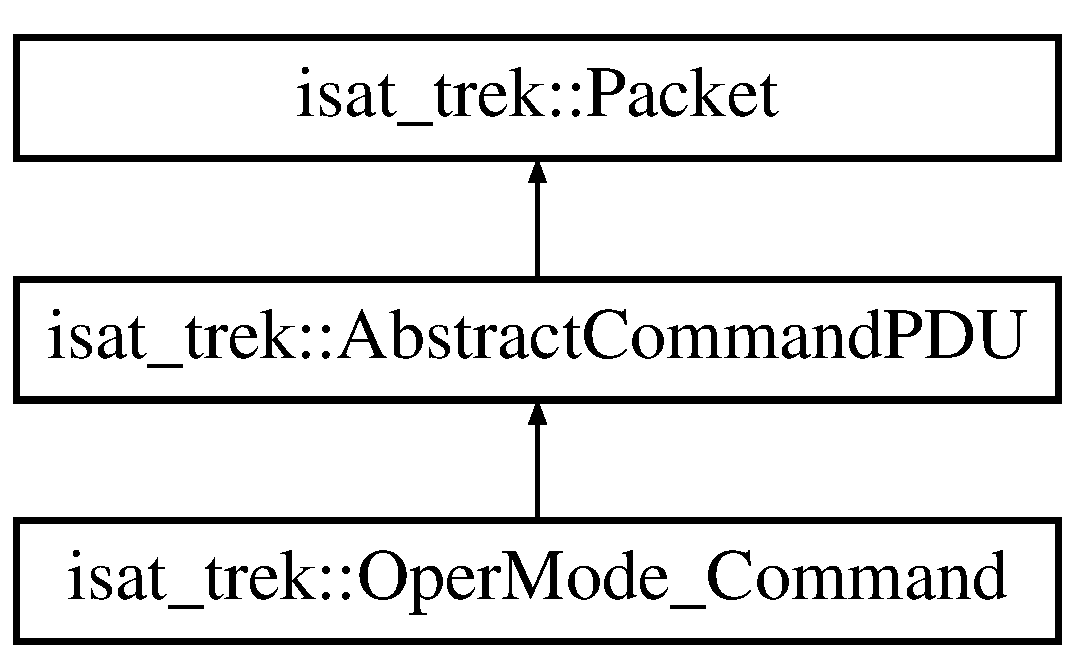
\includegraphics[height=3.000000cm]{classisat__trek_1_1_oper_mode___command}
\end{center}
\end{figure}
\subsection*{Public Member Functions}
\begin{DoxyCompactItemize}
\item 
bool \hyperlink{classisat__trek_1_1_oper_mode___command_a8c075aead046b3ed44127a5d32b8fc91}{from\+Bytes} (Byte\+Buffer \&buf)
\item 
bool \hyperlink{classisat__trek_1_1_oper_mode___command_adddeb62a37efe48bd85fa801067cb970}{to\+Bytes} (Byte\+Buffer \&buf)
\end{DoxyCompactItemize}
\subsection*{Additional Inherited Members}


\subsection{Detailed Description}
X\+XX\+: Replace with real description in isat.\+pdu file. 

\subsection{Member Function Documentation}
\index{isat\+\_\+trek\+::\+Oper\+Mode\+\_\+\+Command@{isat\+\_\+trek\+::\+Oper\+Mode\+\_\+\+Command}!from\+Bytes@{from\+Bytes}}
\index{from\+Bytes@{from\+Bytes}!isat\+\_\+trek\+::\+Oper\+Mode\+\_\+\+Command@{isat\+\_\+trek\+::\+Oper\+Mode\+\_\+\+Command}}
\subsubsection[{\texorpdfstring{from\+Bytes(\+Byte\+Buffer \&buf)}{fromBytes(ByteBuffer &buf)}}]{\setlength{\rightskip}{0pt plus 5cm}bool isat\+\_\+trek\+::\+Oper\+Mode\+\_\+\+Command\+::from\+Bytes (
\begin{DoxyParamCaption}
\item[{Byte\+Buffer \&}]{buf}
\end{DoxyParamCaption}
)\hspace{0.3cm}{\ttfamily [virtual]}}\hypertarget{classisat__trek_1_1_oper_mode___command_a8c075aead046b3ed44127a5d32b8fc91}{}\label{classisat__trek_1_1_oper_mode___command_a8c075aead046b3ed44127a5d32b8fc91}
Populate the header and command fields from the data in buf.

\begin{DoxyReturn}{Returns}
true if successful. 
\end{DoxyReturn}


Implements \hyperlink{classisat__trek_1_1_packet}{isat\+\_\+trek\+::\+Packet}.

\index{isat\+\_\+trek\+::\+Oper\+Mode\+\_\+\+Command@{isat\+\_\+trek\+::\+Oper\+Mode\+\_\+\+Command}!to\+Bytes@{to\+Bytes}}
\index{to\+Bytes@{to\+Bytes}!isat\+\_\+trek\+::\+Oper\+Mode\+\_\+\+Command@{isat\+\_\+trek\+::\+Oper\+Mode\+\_\+\+Command}}
\subsubsection[{\texorpdfstring{to\+Bytes(\+Byte\+Buffer \&buf)}{toBytes(ByteBuffer &buf)}}]{\setlength{\rightskip}{0pt plus 5cm}bool isat\+\_\+trek\+::\+Oper\+Mode\+\_\+\+Command\+::to\+Bytes (
\begin{DoxyParamCaption}
\item[{Byte\+Buffer \&}]{buf}
\end{DoxyParamCaption}
)\hspace{0.3cm}{\ttfamily [virtual]}}\hypertarget{classisat__trek_1_1_oper_mode___command_adddeb62a37efe48bd85fa801067cb970}{}\label{classisat__trek_1_1_oper_mode___command_adddeb62a37efe48bd85fa801067cb970}
Create the binary representation of this instance in the specified buffer.

\begin{DoxyReturn}{Returns}
true if successful. 
\end{DoxyReturn}


Implements \hyperlink{classisat__trek_1_1_packet}{isat\+\_\+trek\+::\+Packet}.



The documentation for this class was generated from the following files\+:\begin{DoxyCompactItemize}
\item 
/home/riley/work/fsw/src/isatgs/\+B\+A\+R\+Co\+Mm\+S/src/dependencies/trek/command/Oper\+Mode\+\_\+\+Command.\+h\item 
/home/riley/work/fsw/src/isatgs/\+B\+A\+R\+Co\+Mm\+S/src/dependencies/trek/command/Oper\+Mode\+\_\+\+Command.\+cpp\end{DoxyCompactItemize}

\hypertarget{class_options}{}\section{Options Class Reference}
\label{class_options}\index{Options@{Options}}
Inheritance diagram for Options\+:\begin{figure}[H]
\begin{center}
\leavevmode
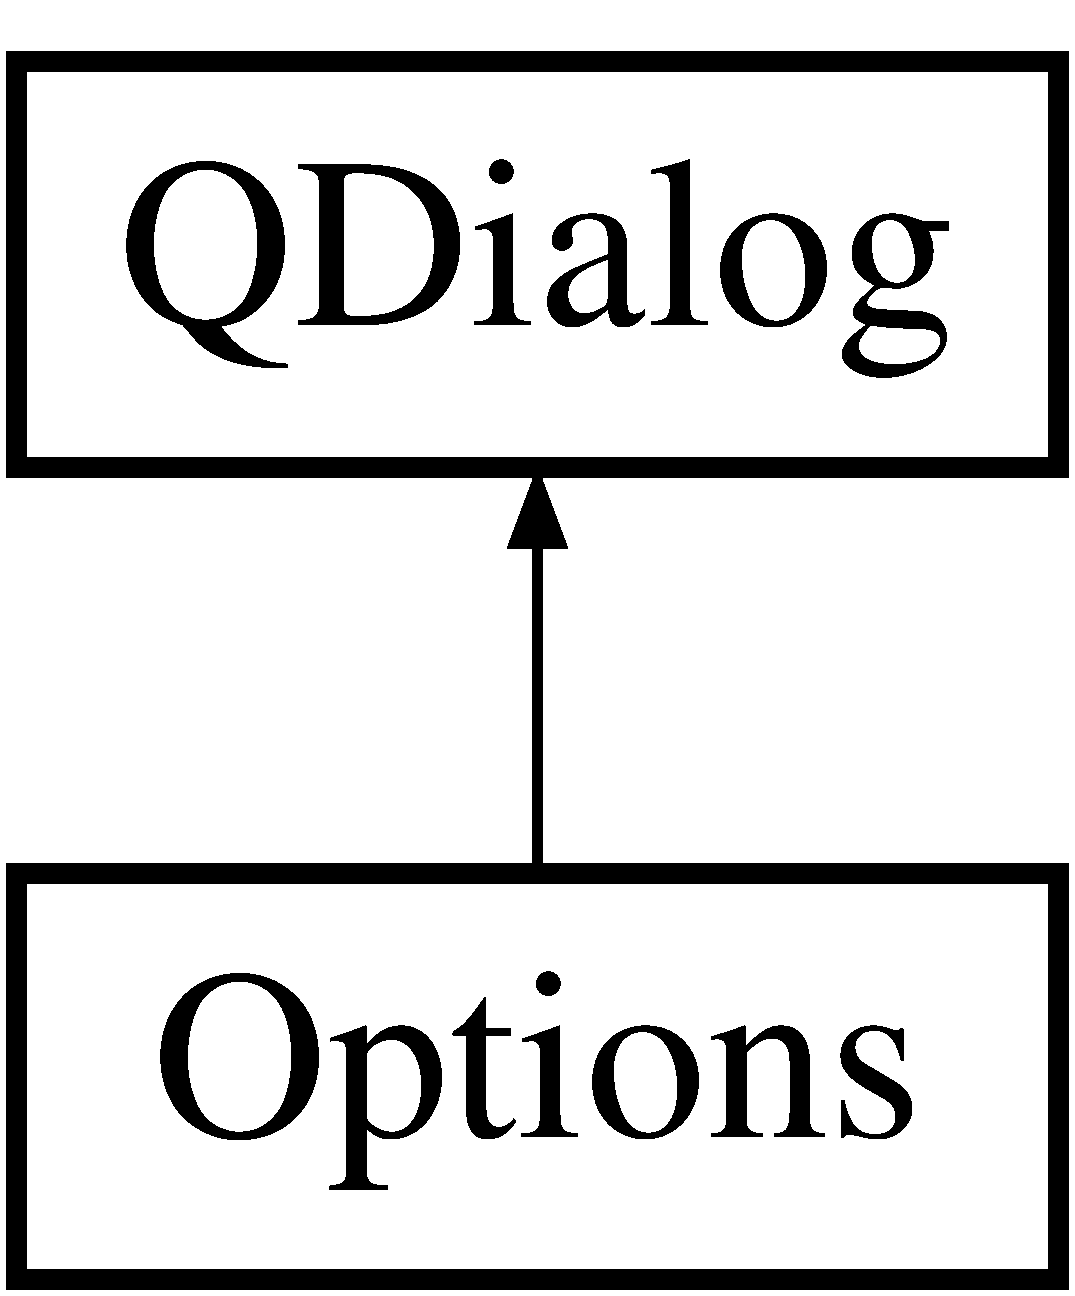
\includegraphics[height=2.000000cm]{class_options}
\end{center}
\end{figure}
\subsection*{Signals}
\begin{DoxyCompactItemize}
\item 
void {\bfseries options\+\_\+modify\+Options} (Q\+String trans\+Type, Q\+String recv\+ID, Q\+String destination)\hypertarget{class_options_a0a4867eb6d4e87ef4281eac680be2820}{}\label{class_options_a0a4867eb6d4e87ef4281eac680be2820}

\end{DoxyCompactItemize}
\subsection*{Public Member Functions}
\begin{DoxyCompactItemize}
\item 
{\bfseries Options} (Q\+Widget $\ast$parent=0)\hypertarget{class_options_a87403ad1d6bd9ae2b54af860bb0f0952}{}\label{class_options_a87403ad1d6bd9ae2b54af860bb0f0952}

\item 
void {\bfseries options\+\_\+change\+Load\+Vals} ()\hypertarget{class_options_afc062573717b1f2598add732d48540e0}{}\label{class_options_afc062573717b1f2598add732d48540e0}

\end{DoxyCompactItemize}
\subsection*{Public Attributes}
\begin{DoxyCompactItemize}
\item 
Q\+String {\bfseries trans\+Type}\hypertarget{class_options_a6f359e34cb5efdf3e24dd0d86fb576f7}{}\label{class_options_a6f359e34cb5efdf3e24dd0d86fb576f7}

\item 
Q\+String {\bfseries recv\+ID}\hypertarget{class_options_ac3bb77e29ee6b4910bc2406c66963919}{}\label{class_options_ac3bb77e29ee6b4910bc2406c66963919}

\item 
Q\+String {\bfseries destination}\hypertarget{class_options_a882d6e77af04ab32704e0add17079268}{}\label{class_options_a882d6e77af04ab32704e0add17079268}

\end{DoxyCompactItemize}


The documentation for this class was generated from the following files\+:\begin{DoxyCompactItemize}
\item 
/home/riley/work/fsw/src/isatgs/\+B\+A\+R\+Co\+Mm\+S/src/modules/\+B\+A\+R\+Co\+Mm\+S\+\_\+\+C\+F\+D\+P/options.\+h\item 
/home/riley/work/fsw/src/isatgs/\+B\+A\+R\+Co\+Mm\+S/src/modules/\+B\+A\+R\+Co\+Mm\+S\+\_\+\+C\+F\+D\+P/options.\+cpp\end{DoxyCompactItemize}

\hypertarget{structisat__utils_1_1_event_database_1_1_origin}{}\section{isat\+\_\+utils\+:\+:Event\+Database\+:\+:Origin Struct Reference}
\label{structisat__utils_1_1_event_database_1_1_origin}\index{isat\+\_\+utils\+::\+Event\+Database\+::\+Origin@{isat\+\_\+utils\+::\+Event\+Database\+::\+Origin}}
\subsection*{Public Attributes}
\begin{DoxyCompactItemize}
\item 
int {\bfseries code}\hypertarget{structisat__utils_1_1_event_database_1_1_origin_af71fc5f8872ff29e914b6964ed743971}{}\label{structisat__utils_1_1_event_database_1_1_origin_af71fc5f8872ff29e914b6964ed743971}

\item 
std\+::string {\bfseries name}\hypertarget{structisat__utils_1_1_event_database_1_1_origin_adf4bfbcf38089389c5664ef9bf8c95f8}{}\label{structisat__utils_1_1_event_database_1_1_origin_adf4bfbcf38089389c5664ef9bf8c95f8}

\end{DoxyCompactItemize}


The documentation for this struct was generated from the following file\+:\begin{DoxyCompactItemize}
\item 
/home/riley/work/fsw/src/isatgs/\+B\+A\+R\+Co\+Mm\+S/src/dependencies/utils/Event\+Database.\+h\end{DoxyCompactItemize}

\hypertarget{class_output}{}\section{Output Class Reference}
\label{class_output}\index{Output@{Output}}
Inheritance diagram for Output\+:\begin{figure}[H]
\begin{center}
\leavevmode
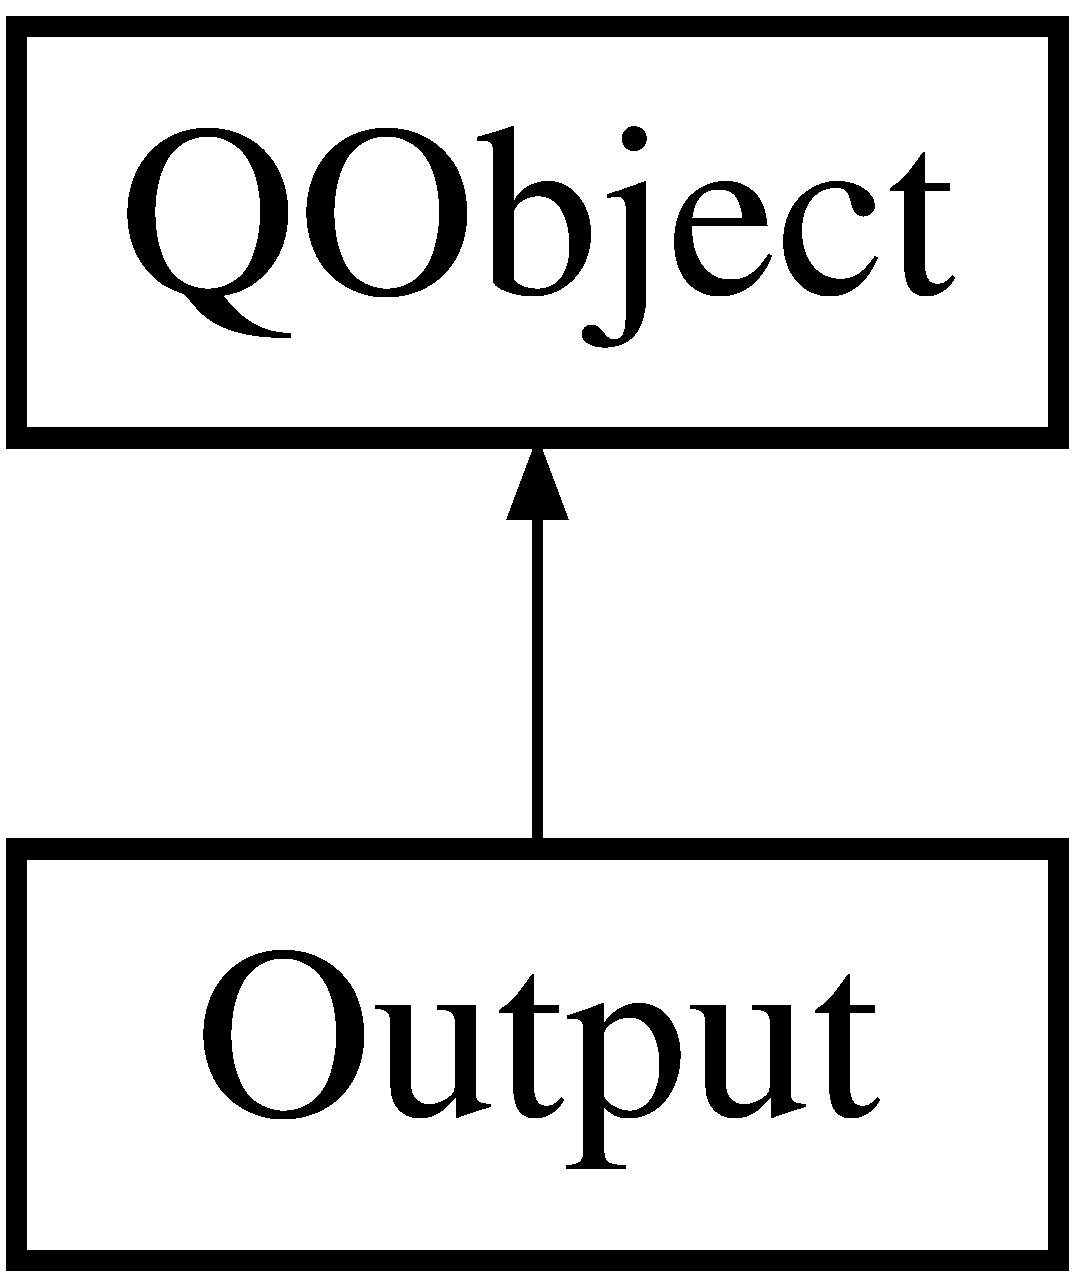
\includegraphics[height=2.000000cm]{class_output}
\end{center}
\end{figure}
\subsection*{Signals}
\begin{DoxyCompactItemize}
\item 
void {\bfseries output\+\_\+append\+Output} (char $\ast$str)\hypertarget{class_output_a7fedf8dc52fa6244c72b7ccc6fa87a3d}{}\label{class_output_a7fedf8dc52fa6244c72b7ccc6fa87a3d}

\end{DoxyCompactItemize}
\subsection*{Public Member Functions}
\begin{DoxyCompactItemize}
\item 
void {\bfseries printer} (char $\ast$str)\hypertarget{class_output_a1284884752d63797713902db09b9de04}{}\label{class_output_a1284884752d63797713902db09b9de04}

\end{DoxyCompactItemize}


The documentation for this class was generated from the following files\+:\begin{DoxyCompactItemize}
\item 
/home/riley/work/fsw/src/isatgs/\+B\+A\+R\+Co\+Mm\+S/src/modules/\+B\+A\+R\+Co\+Mm\+S\+\_\+\+C\+F\+D\+P/output.\+h\item 
/home/riley/work/fsw/src/isatgs/\+B\+A\+R\+Co\+Mm\+S/src/modules/\+B\+A\+R\+Co\+Mm\+S\+\_\+\+C\+F\+D\+P/output.\+cpp\end{DoxyCompactItemize}

\hypertarget{classisat__trek_1_1_packet}{}\section{isat\+\_\+trek\+:\+:Packet Class Reference}
\label{classisat__trek_1_1_packet}\index{isat\+\_\+trek\+::\+Packet@{isat\+\_\+trek\+::\+Packet}}
Inheritance diagram for isat\+\_\+trek\+:\+:Packet\+:\begin{figure}[H]
\begin{center}
\leavevmode
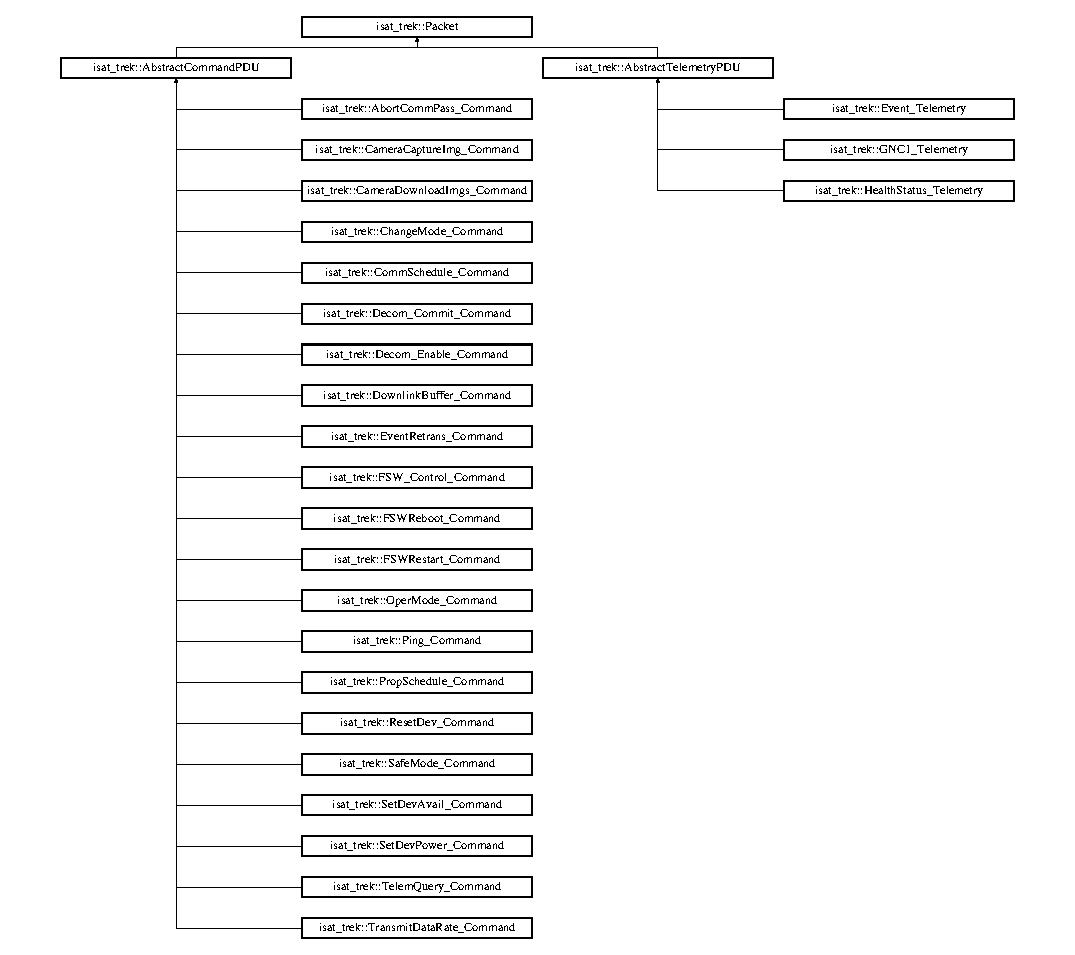
\includegraphics[height=12.000000cm]{classisat__trek_1_1_packet}
\end{center}
\end{figure}
\subsection*{Public Member Functions}
\begin{DoxyCompactItemize}
\item 
virtual bool {\bfseries to\+Bytes} (\hyperlink{classisat__utils_1_1_byte_buffer}{Byte\+Buffer} \&buf)=0\hypertarget{classisat__trek_1_1_packet_a51c8893a9eaf7e234474f9555d0af87c}{}\label{classisat__trek_1_1_packet_a51c8893a9eaf7e234474f9555d0af87c}

\item 
virtual bool {\bfseries from\+Bytes} (\hyperlink{classisat__utils_1_1_byte_buffer}{Byte\+Buffer} \&buf)=0\hypertarget{classisat__trek_1_1_packet_abc0b9e0fc84e4cc2e49fcf262f50ee2e}{}\label{classisat__trek_1_1_packet_abc0b9e0fc84e4cc2e49fcf262f50ee2e}

\end{DoxyCompactItemize}


The documentation for this class was generated from the following file\+:\begin{DoxyCompactItemize}
\item 
/home/riley/work/fsw/src/isatgs/\+B\+A\+R\+Co\+Mm\+S/src/dependencies/trek/Packet.\+h\end{DoxyCompactItemize}

\hypertarget{class_p_d_u}{}\section{P\+DU Class Reference}
\label{class_p_d_u}\index{P\+DU@{P\+DU}}
\subsection*{Public Attributes}
\begin{DoxyCompactItemize}
\item 
\hyperlink{classisat__net_1_1_end_point}{End\+Point} {\bfseries source}\hypertarget{class_p_d_u_af2103f3da8de41d94a423b2e2f99fb4e}{}\label{class_p_d_u_af2103f3da8de41d94a423b2e2f99fb4e}

\item 
\hyperlink{classisat__net_1_1_end_point}{End\+Point} {\bfseries destination}\hypertarget{class_p_d_u_a7dbc2c8b12d0e1b6f7dae1dccde4f8d8}{}\label{class_p_d_u_a7dbc2c8b12d0e1b6f7dae1dccde4f8d8}

\item 
Byte\+Buffer {\bfseries data}\hypertarget{class_p_d_u_aed2fc032220544e55800cde2d58db0b2}{}\label{class_p_d_u_aed2fc032220544e55800cde2d58db0b2}

\end{DoxyCompactItemize}


The documentation for this class was generated from the following file\+:\begin{DoxyCompactItemize}
\item 
/home/riley/work/fsw/src/isatgs/\+B\+A\+R\+Co\+Mm\+S/src/dependencies/net/P\+D\+U.\+h\end{DoxyCompactItemize}

\hypertarget{struct_p_d_u___a_s___s_t_r_u_c_t}{}\section{P\+D\+U\+\_\+\+A\+S\+\_\+\+S\+T\+R\+U\+CT Struct Reference}
\label{struct_p_d_u___a_s___s_t_r_u_c_t}\index{P\+D\+U\+\_\+\+A\+S\+\_\+\+S\+T\+R\+U\+CT@{P\+D\+U\+\_\+\+A\+S\+\_\+\+S\+T\+R\+U\+CT}}
\subsection*{Public Attributes}
\begin{DoxyCompactItemize}
\item 
\hyperlink{struct_h_d_r}{H\+DR} {\bfseries hdr}\hypertarget{struct_p_d_u___a_s___s_t_r_u_c_t_a21f7c85339c5f28da0b572896c455188}{}\label{struct_p_d_u___a_s___s_t_r_u_c_t_a21f7c85339c5f28da0b572896c455188}

\item 
boolean {\bfseries is\+\_\+this\+\_\+a\+\_\+file\+\_\+data\+\_\+pdu}\hypertarget{struct_p_d_u___a_s___s_t_r_u_c_t_a0c1b743b813bc863e4f7052275cee968}{}\label{struct_p_d_u___a_s___s_t_r_u_c_t_a0c1b743b813bc863e4f7052275cee968}

\item 
F\+I\+L\+E\+\_\+\+D\+I\+R\+\_\+\+C\+O\+DE {\bfseries dir\+\_\+code}\hypertarget{struct_p_d_u___a_s___s_t_r_u_c_t_a8a7f600e62d176b8f3054e80327fc829}{}\label{struct_p_d_u___a_s___s_t_r_u_c_t_a8a7f600e62d176b8f3054e80327fc829}

\item 
\hyperlink{union_d_a_t_a___f_i_e_l_d}{D\+A\+T\+A\+\_\+\+F\+I\+E\+LD} {\bfseries data\+\_\+field}\hypertarget{struct_p_d_u___a_s___s_t_r_u_c_t_aaf9727776981c70e7e4d67ab30c70aec}{}\label{struct_p_d_u___a_s___s_t_r_u_c_t_aaf9727776981c70e7e4d67ab30c70aec}

\end{DoxyCompactItemize}


The documentation for this struct was generated from the following file\+:\begin{DoxyCompactItemize}
\item 
/home/riley/work/fsw/src/isatgs/\+B\+A\+R\+Co\+Mm\+S/src/dependencies/\+C\+F\+D\+P/\+P\+R\+I/structures.\+h\end{DoxyCompactItemize}

\hypertarget{struct_p_d_u___l_a_y_o_u_t}{}\section{P\+D\+U\+\_\+\+L\+A\+Y\+O\+UT Struct Reference}
\label{struct_p_d_u___l_a_y_o_u_t}\index{P\+D\+U\+\_\+\+L\+A\+Y\+O\+UT@{P\+D\+U\+\_\+\+L\+A\+Y\+O\+UT}}
\subsection*{Public Attributes}
\begin{DoxyCompactItemize}
\item 
int {\bfseries start\+\_\+of\+\_\+source\+\_\+id}\hypertarget{struct_p_d_u___l_a_y_o_u_t_a043cb581971314420aa4e56f28caf3c0}{}\label{struct_p_d_u___l_a_y_o_u_t_a043cb581971314420aa4e56f28caf3c0}

\item 
u\+\_\+int\+\_\+1 {\bfseries length\+\_\+of\+\_\+source\+\_\+id}\hypertarget{struct_p_d_u___l_a_y_o_u_t_af8e6be27a8f640bb5375bc5309990981}{}\label{struct_p_d_u___l_a_y_o_u_t_af8e6be27a8f640bb5375bc5309990981}

\item 
int {\bfseries start\+\_\+of\+\_\+trans\+\_\+seq\+\_\+num}\hypertarget{struct_p_d_u___l_a_y_o_u_t_a2a2e3ff07e91173db7fb6235ea71d04c}{}\label{struct_p_d_u___l_a_y_o_u_t_a2a2e3ff07e91173db7fb6235ea71d04c}

\item 
u\+\_\+int\+\_\+1 {\bfseries length\+\_\+of\+\_\+trans\+\_\+seq\+\_\+num}\hypertarget{struct_p_d_u___l_a_y_o_u_t_a6b7363e84bc3da85a9f2b950dc0b578b}{}\label{struct_p_d_u___l_a_y_o_u_t_a6b7363e84bc3da85a9f2b950dc0b578b}

\item 
int {\bfseries start\+\_\+of\+\_\+dest\+\_\+id}\hypertarget{struct_p_d_u___l_a_y_o_u_t_a6a72eceded37c912aa93dd01c45ebf36}{}\label{struct_p_d_u___l_a_y_o_u_t_a6a72eceded37c912aa93dd01c45ebf36}

\item 
u\+\_\+int\+\_\+1 {\bfseries length\+\_\+of\+\_\+dest\+\_\+id}\hypertarget{struct_p_d_u___l_a_y_o_u_t_a93cc676237ae77ad7cf7a126a01634a5}{}\label{struct_p_d_u___l_a_y_o_u_t_a93cc676237ae77ad7cf7a126a01634a5}

\item 
int {\bfseries length\+\_\+of\+\_\+header}\hypertarget{struct_p_d_u___l_a_y_o_u_t_a7c0d51316eb33fe724bfd0f296d1f736}{}\label{struct_p_d_u___l_a_y_o_u_t_a7c0d51316eb33fe724bfd0f296d1f736}

\end{DoxyCompactItemize}


The documentation for this struct was generated from the following file\+:\begin{DoxyCompactItemize}
\item 
/home/riley/work/fsw/src/isatgs/\+B\+A\+R\+Co\+Mm\+S/src/dependencies/\+C\+F\+D\+P/\+P\+R\+I/pdu.\+c\end{DoxyCompactItemize}

\hypertarget{classisat__trek_1_1_ping___command}{}\section{isat\+\_\+trek\+:\+:Ping\+\_\+\+Command Class Reference}
\label{classisat__trek_1_1_ping___command}\index{isat\+\_\+trek\+::\+Ping\+\_\+\+Command@{isat\+\_\+trek\+::\+Ping\+\_\+\+Command}}


{\ttfamily \#include $<$Ping\+\_\+\+Command.\+h$>$}

Inheritance diagram for isat\+\_\+trek\+:\+:Ping\+\_\+\+Command\+:\begin{figure}[H]
\begin{center}
\leavevmode
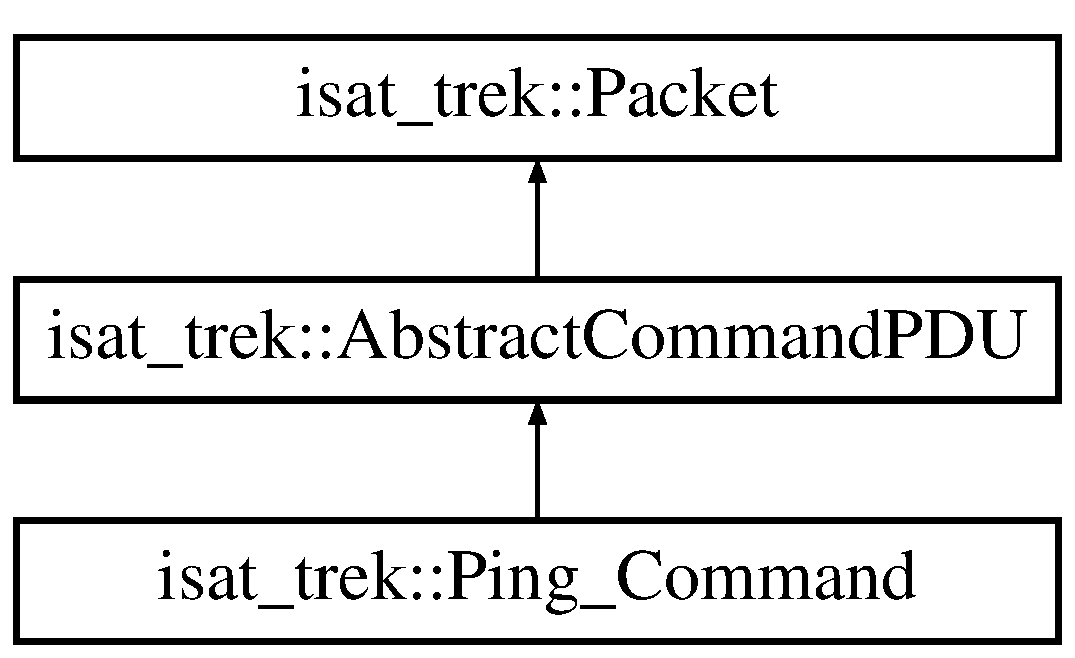
\includegraphics[height=3.000000cm]{classisat__trek_1_1_ping___command}
\end{center}
\end{figure}
\subsection*{Public Member Functions}
\begin{DoxyCompactItemize}
\item 
bool \hyperlink{classisat__trek_1_1_ping___command_afff4dc8927c1f4f729b2869b88e51cf8}{from\+Bytes} (Byte\+Buffer \&buf)
\item 
bool \hyperlink{classisat__trek_1_1_ping___command_a70eb1b308108360bcddef7263d99700e}{to\+Bytes} (Byte\+Buffer \&buf)
\end{DoxyCompactItemize}
\subsection*{Additional Inherited Members}


\subsection{Detailed Description}
X\+XX\+: Replace with real description in isat.\+pdu file. 

\subsection{Member Function Documentation}
\index{isat\+\_\+trek\+::\+Ping\+\_\+\+Command@{isat\+\_\+trek\+::\+Ping\+\_\+\+Command}!from\+Bytes@{from\+Bytes}}
\index{from\+Bytes@{from\+Bytes}!isat\+\_\+trek\+::\+Ping\+\_\+\+Command@{isat\+\_\+trek\+::\+Ping\+\_\+\+Command}}
\subsubsection[{\texorpdfstring{from\+Bytes(\+Byte\+Buffer \&buf)}{fromBytes(ByteBuffer &buf)}}]{\setlength{\rightskip}{0pt plus 5cm}bool isat\+\_\+trek\+::\+Ping\+\_\+\+Command\+::from\+Bytes (
\begin{DoxyParamCaption}
\item[{Byte\+Buffer \&}]{buf}
\end{DoxyParamCaption}
)\hspace{0.3cm}{\ttfamily [virtual]}}\hypertarget{classisat__trek_1_1_ping___command_afff4dc8927c1f4f729b2869b88e51cf8}{}\label{classisat__trek_1_1_ping___command_afff4dc8927c1f4f729b2869b88e51cf8}
Populate the header and command fields from the data in buf.

\begin{DoxyReturn}{Returns}
true if successful. 
\end{DoxyReturn}


Implements \hyperlink{classisat__trek_1_1_packet}{isat\+\_\+trek\+::\+Packet}.

\index{isat\+\_\+trek\+::\+Ping\+\_\+\+Command@{isat\+\_\+trek\+::\+Ping\+\_\+\+Command}!to\+Bytes@{to\+Bytes}}
\index{to\+Bytes@{to\+Bytes}!isat\+\_\+trek\+::\+Ping\+\_\+\+Command@{isat\+\_\+trek\+::\+Ping\+\_\+\+Command}}
\subsubsection[{\texorpdfstring{to\+Bytes(\+Byte\+Buffer \&buf)}{toBytes(ByteBuffer &buf)}}]{\setlength{\rightskip}{0pt plus 5cm}bool isat\+\_\+trek\+::\+Ping\+\_\+\+Command\+::to\+Bytes (
\begin{DoxyParamCaption}
\item[{Byte\+Buffer \&}]{buf}
\end{DoxyParamCaption}
)\hspace{0.3cm}{\ttfamily [virtual]}}\hypertarget{classisat__trek_1_1_ping___command_a70eb1b308108360bcddef7263d99700e}{}\label{classisat__trek_1_1_ping___command_a70eb1b308108360bcddef7263d99700e}
Create the binary representation of this instance in the specified buffer.

\begin{DoxyReturn}{Returns}
true if successful. 
\end{DoxyReturn}


Implements \hyperlink{classisat__trek_1_1_packet}{isat\+\_\+trek\+::\+Packet}.



The documentation for this class was generated from the following files\+:\begin{DoxyCompactItemize}
\item 
/home/riley/work/fsw/src/isatgs/\+B\+A\+R\+Co\+Mm\+S/src/dependencies/trek/command/Ping\+\_\+\+Command.\+h\item 
/home/riley/work/fsw/src/isatgs/\+B\+A\+R\+Co\+Mm\+S/src/dependencies/trek/command/Ping\+\_\+\+Command.\+cpp\end{DoxyCompactItemize}

\hypertarget{classisat__trek_1_1_prop_schedule___command}{}\section{isat\+\_\+trek\+:\+:Prop\+Schedule\+\_\+\+Command Class Reference}
\label{classisat__trek_1_1_prop_schedule___command}\index{isat\+\_\+trek\+::\+Prop\+Schedule\+\_\+\+Command@{isat\+\_\+trek\+::\+Prop\+Schedule\+\_\+\+Command}}


{\ttfamily \#include $<$Prop\+Schedule\+\_\+\+Command.\+h$>$}

Inheritance diagram for isat\+\_\+trek\+:\+:Prop\+Schedule\+\_\+\+Command\+:\begin{figure}[H]
\begin{center}
\leavevmode
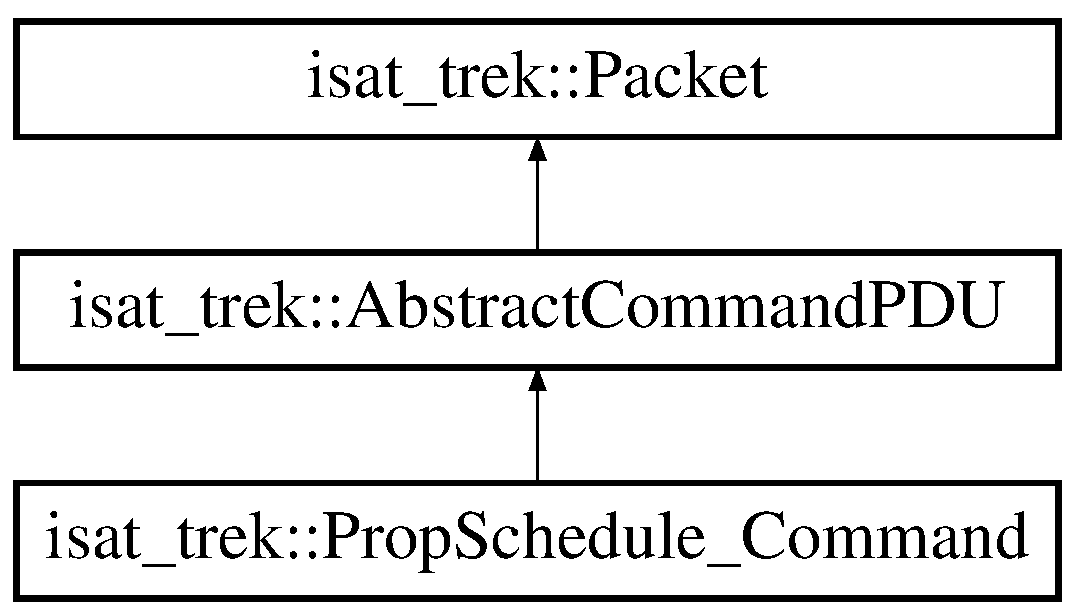
\includegraphics[height=3.000000cm]{classisat__trek_1_1_prop_schedule___command}
\end{center}
\end{figure}
\subsection*{Public Member Functions}
\begin{DoxyCompactItemize}
\item 
bool \hyperlink{classisat__trek_1_1_prop_schedule___command_af86e57e6f65f6d2a977b082c1f69be09}{from\+Bytes} (Byte\+Buffer \&buf)
\item 
bool \hyperlink{classisat__trek_1_1_prop_schedule___command_a0c18c7191323e932b7c30f9115c059ee}{to\+Bytes} (Byte\+Buffer \&buf)
\end{DoxyCompactItemize}
\subsection*{Additional Inherited Members}


\subsection{Detailed Description}
X\+XX\+: Replace with real description in isat.\+pdu file. 

\subsection{Member Function Documentation}
\index{isat\+\_\+trek\+::\+Prop\+Schedule\+\_\+\+Command@{isat\+\_\+trek\+::\+Prop\+Schedule\+\_\+\+Command}!from\+Bytes@{from\+Bytes}}
\index{from\+Bytes@{from\+Bytes}!isat\+\_\+trek\+::\+Prop\+Schedule\+\_\+\+Command@{isat\+\_\+trek\+::\+Prop\+Schedule\+\_\+\+Command}}
\subsubsection[{\texorpdfstring{from\+Bytes(\+Byte\+Buffer \&buf)}{fromBytes(ByteBuffer &buf)}}]{\setlength{\rightskip}{0pt plus 5cm}bool isat\+\_\+trek\+::\+Prop\+Schedule\+\_\+\+Command\+::from\+Bytes (
\begin{DoxyParamCaption}
\item[{Byte\+Buffer \&}]{buf}
\end{DoxyParamCaption}
)\hspace{0.3cm}{\ttfamily [virtual]}}\hypertarget{classisat__trek_1_1_prop_schedule___command_af86e57e6f65f6d2a977b082c1f69be09}{}\label{classisat__trek_1_1_prop_schedule___command_af86e57e6f65f6d2a977b082c1f69be09}
Populate the header and command fields from the data in buf.

\begin{DoxyReturn}{Returns}
true if successful. 
\end{DoxyReturn}


Implements \hyperlink{classisat__trek_1_1_packet}{isat\+\_\+trek\+::\+Packet}.

\index{isat\+\_\+trek\+::\+Prop\+Schedule\+\_\+\+Command@{isat\+\_\+trek\+::\+Prop\+Schedule\+\_\+\+Command}!to\+Bytes@{to\+Bytes}}
\index{to\+Bytes@{to\+Bytes}!isat\+\_\+trek\+::\+Prop\+Schedule\+\_\+\+Command@{isat\+\_\+trek\+::\+Prop\+Schedule\+\_\+\+Command}}
\subsubsection[{\texorpdfstring{to\+Bytes(\+Byte\+Buffer \&buf)}{toBytes(ByteBuffer &buf)}}]{\setlength{\rightskip}{0pt plus 5cm}bool isat\+\_\+trek\+::\+Prop\+Schedule\+\_\+\+Command\+::to\+Bytes (
\begin{DoxyParamCaption}
\item[{Byte\+Buffer \&}]{buf}
\end{DoxyParamCaption}
)\hspace{0.3cm}{\ttfamily [virtual]}}\hypertarget{classisat__trek_1_1_prop_schedule___command_a0c18c7191323e932b7c30f9115c059ee}{}\label{classisat__trek_1_1_prop_schedule___command_a0c18c7191323e932b7c30f9115c059ee}
Create the binary representation of this instance in the specified buffer.

\begin{DoxyReturn}{Returns}
true if successful. 
\end{DoxyReturn}


Implements \hyperlink{classisat__trek_1_1_packet}{isat\+\_\+trek\+::\+Packet}.



The documentation for this class was generated from the following files\+:\begin{DoxyCompactItemize}
\item 
/home/riley/work/fsw/src/isatgs/\+B\+A\+R\+Co\+Mm\+S/src/dependencies/trek/command/Prop\+Schedule\+\_\+\+Command.\+h\item 
/home/riley/work/fsw/src/isatgs/\+B\+A\+R\+Co\+Mm\+S/src/dependencies/trek/command/Prop\+Schedule\+\_\+\+Command.\+cpp\end{DoxyCompactItemize}

\hypertarget{struct_p_u_t___i_n_f_o}{}\section{P\+U\+T\+\_\+\+I\+N\+FO Struct Reference}
\label{struct_p_u_t___i_n_f_o}\index{P\+U\+T\+\_\+\+I\+N\+FO@{P\+U\+T\+\_\+\+I\+N\+FO}}
\subsection*{Public Attributes}
\begin{DoxyCompactItemize}
\item 
boolean {\bfseries ack\+\_\+required}\hypertarget{struct_p_u_t___i_n_f_o_a8d8458d6859cab3494bd8d75193cdba2}{}\label{struct_p_u_t___i_n_f_o_a8d8458d6859cab3494bd8d75193cdba2}

\item 
\hyperlink{struct_i_d}{ID} {\bfseries dest\+\_\+id}\hypertarget{struct_p_u_t___i_n_f_o_a6808d22b94b57c69105a09664eb0d7cc}{}\label{struct_p_u_t___i_n_f_o_a6808d22b94b57c69105a09664eb0d7cc}

\item 
boolean {\bfseries file\+\_\+transfer}\hypertarget{struct_p_u_t___i_n_f_o_a0f1fe47d2a56a42265ff65a6aa287467}{}\label{struct_p_u_t___i_n_f_o_a0f1fe47d2a56a42265ff65a6aa287467}

\item 
char {\bfseries source\+\_\+file\+\_\+name} \mbox{[}M\+A\+X\+\_\+\+F\+I\+L\+E\+\_\+\+N\+A\+M\+E\+\_\+\+L\+E\+N\+G\+TH+1\mbox{]}\hypertarget{struct_p_u_t___i_n_f_o_a324d49720dfd1891abb344bd89e90487}{}\label{struct_p_u_t___i_n_f_o_a324d49720dfd1891abb344bd89e90487}

\item 
char {\bfseries dest\+\_\+file\+\_\+name} \mbox{[}M\+A\+X\+\_\+\+F\+I\+L\+E\+\_\+\+N\+A\+M\+E\+\_\+\+L\+E\+N\+G\+TH+1\mbox{]}\hypertarget{struct_p_u_t___i_n_f_o_abad4d56f97566b50d27e3cb91265d558}{}\label{struct_p_u_t___i_n_f_o_abad4d56f97566b50d27e3cb91265d558}

\end{DoxyCompactItemize}


The documentation for this struct was generated from the following file\+:\begin{DoxyCompactItemize}
\item 
/home/riley/work/fsw/src/isatgs/\+B\+A\+R\+Co\+Mm\+S/src/dependencies/\+C\+F\+D\+P/\+P\+R\+I/structures.\+h\end{DoxyCompactItemize}

\hypertarget{struct_r_e_q_u_e_s_t}{}\section{R\+E\+Q\+U\+E\+ST Struct Reference}
\label{struct_r_e_q_u_e_s_t}\index{R\+E\+Q\+U\+E\+ST@{R\+E\+Q\+U\+E\+ST}}
\subsection*{Public Attributes}
\begin{DoxyCompactItemize}
\item 
R\+E\+Q\+U\+E\+S\+T\+\_\+\+T\+Y\+PE {\bfseries type}\hypertarget{struct_r_e_q_u_e_s_t_a0f5230fb19c5a4616098460a082d2f3a}{}\label{struct_r_e_q_u_e_s_t_a0f5230fb19c5a4616098460a082d2f3a}

\item 
\begin{tabbing}
xx\=xx\=xx\=xx\=xx\=xx\=xx\=xx\=xx\=\kill
union \{\\
\>\hyperlink{struct_p_u_t___i_n_f_o}{PUT\_INFO} {\bfseries put}\\
\>\hyperlink{struct_t_r_a_n_s_a_c_t_i_o_n}{TRANSACTION} {\bfseries trans}\\
\} {\bfseries info}\hypertarget{struct_r_e_q_u_e_s_t_afbdff347471ad0aafd436ce9679aafa4}{}\label{struct_r_e_q_u_e_s_t_afbdff347471ad0aafd436ce9679aafa4}
\\

\end{tabbing}\end{DoxyCompactItemize}


The documentation for this struct was generated from the following file\+:\begin{DoxyCompactItemize}
\item 
/home/riley/work/fsw/src/isatgs/\+B\+A\+R\+Co\+Mm\+S/src/dependencies/\+C\+F\+D\+P/\+P\+R\+I/structures.\+h\end{DoxyCompactItemize}

\hypertarget{class_requests}{}\section{Requests Class Reference}
\label{class_requests}\index{Requests@{Requests}}
Inheritance diagram for Requests\+:\begin{figure}[H]
\begin{center}
\leavevmode
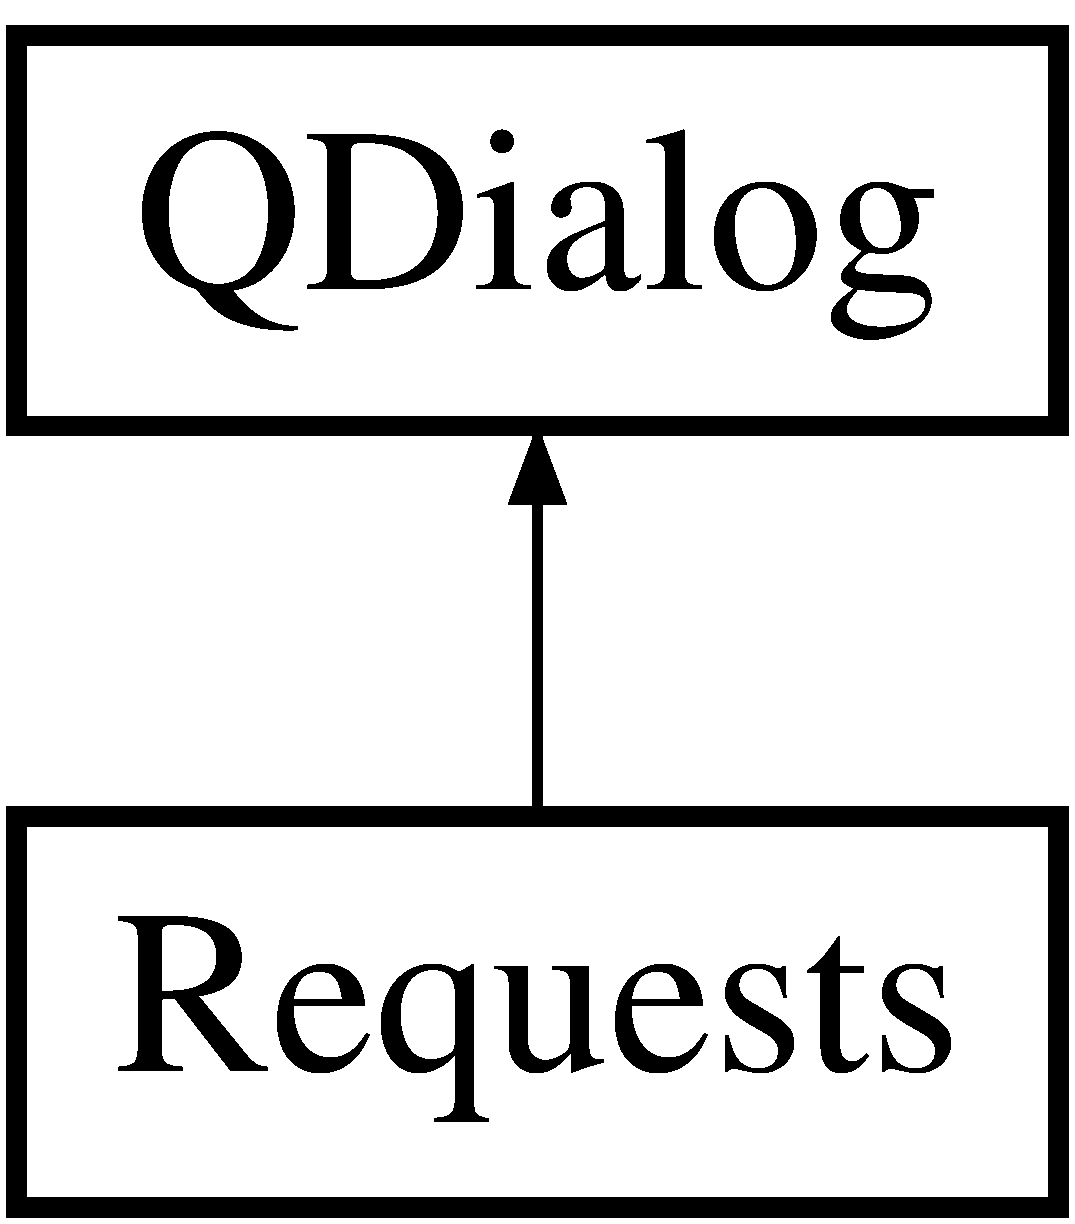
\includegraphics[height=2.000000cm]{class_requests}
\end{center}
\end{figure}
\subsection*{Signals}
\begin{DoxyCompactItemize}
\item 
void {\bfseries requests\+\_\+append\+Output} (std\+::vector$<$ std\+::string $>$ requests)\hypertarget{class_requests_a3221858d3e1462d504bb1f64d84701c0}{}\label{class_requests_a3221858d3e1462d504bb1f64d84701c0}

\end{DoxyCompactItemize}
\subsection*{Public Member Functions}
\begin{DoxyCompactItemize}
\item 
{\bfseries Requests} (Q\+Widget $\ast$parent=0)\hypertarget{class_requests_a26026f2733a6fca27d1f3d85d2a92602}{}\label{class_requests_a26026f2733a6fca27d1f3d85d2a92602}

\item 
void {\bfseries initialize\+Form} (Q\+String title, Q\+String description, Q\+String request)\hypertarget{class_requests_a7e5fcc23aab5ddfe778d4fb008d427a4}{}\label{class_requests_a7e5fcc23aab5ddfe778d4fb008d427a4}

\end{DoxyCompactItemize}


The documentation for this class was generated from the following files\+:\begin{DoxyCompactItemize}
\item 
/home/riley/work/fsw/src/isatgs/\+B\+A\+R\+Co\+Mm\+S/src/modules/\+B\+A\+R\+Co\+Mm\+S\+\_\+\+C\+F\+D\+P/requests.\+h\item 
/home/riley/work/fsw/src/isatgs/\+B\+A\+R\+Co\+Mm\+S/src/modules/\+B\+A\+R\+Co\+Mm\+S\+\_\+\+C\+F\+D\+P/requests.\+cpp\end{DoxyCompactItemize}

\hypertarget{classisat__trek_1_1_reset_dev___command}{}\section{isat\+\_\+trek\+:\+:Reset\+Dev\+\_\+\+Command Class Reference}
\label{classisat__trek_1_1_reset_dev___command}\index{isat\+\_\+trek\+::\+Reset\+Dev\+\_\+\+Command@{isat\+\_\+trek\+::\+Reset\+Dev\+\_\+\+Command}}


{\ttfamily \#include $<$Reset\+Dev\+\_\+\+Command.\+h$>$}

Inheritance diagram for isat\+\_\+trek\+:\+:Reset\+Dev\+\_\+\+Command\+:\begin{figure}[H]
\begin{center}
\leavevmode
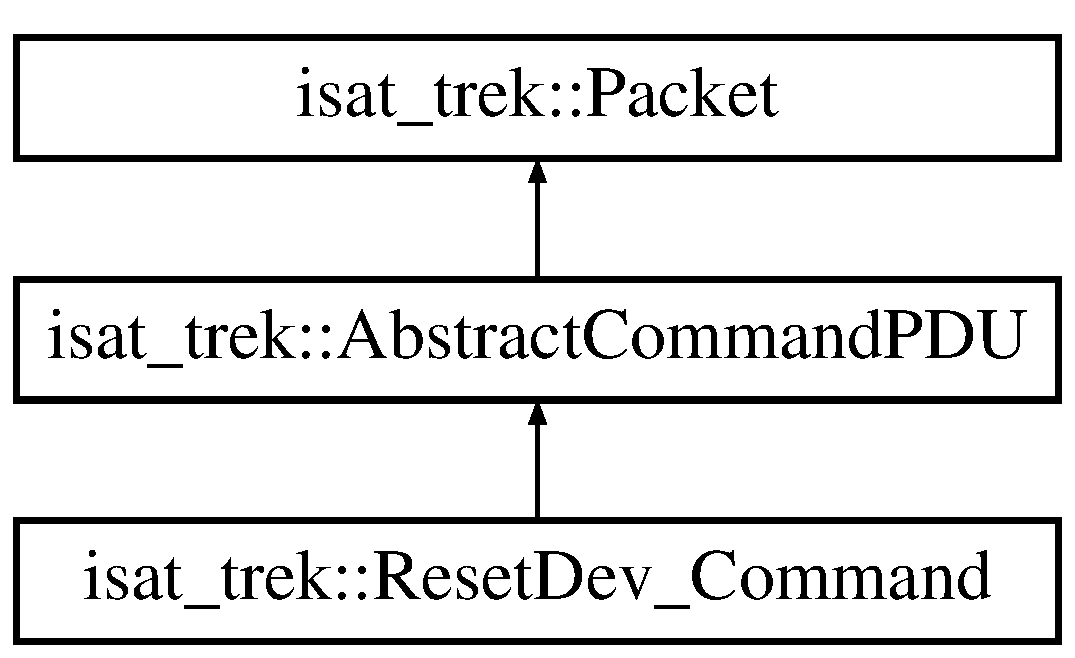
\includegraphics[height=3.000000cm]{classisat__trek_1_1_reset_dev___command}
\end{center}
\end{figure}
\subsection*{Public Member Functions}
\begin{DoxyCompactItemize}
\item 
bool \hyperlink{classisat__trek_1_1_reset_dev___command_a5d86014da142b8de868eff133eb1caef}{from\+Bytes} (Byte\+Buffer \&buf)
\item 
bool \hyperlink{classisat__trek_1_1_reset_dev___command_acbda631f644d4e9edfada832f4d7619c}{to\+Bytes} (Byte\+Buffer \&buf)
\end{DoxyCompactItemize}
\subsection*{Public Attributes}
\begin{DoxyCompactItemize}
\item 
int {\bfseries device} = 0\hypertarget{classisat__trek_1_1_reset_dev___command_ae6fce49cf8031c4d862809dccab9884f}{}\label{classisat__trek_1_1_reset_dev___command_ae6fce49cf8031c4d862809dccab9884f}

\item 
int {\bfseries cycle\+Time} = 0\hypertarget{classisat__trek_1_1_reset_dev___command_a5fcebe9400f435caa5dd63bc3cad94af}{}\label{classisat__trek_1_1_reset_dev___command_a5fcebe9400f435caa5dd63bc3cad94af}

\end{DoxyCompactItemize}


\subsection{Detailed Description}
X\+XX\+: Replace with real description in isat.\+pdu file. 

\subsection{Member Function Documentation}
\index{isat\+\_\+trek\+::\+Reset\+Dev\+\_\+\+Command@{isat\+\_\+trek\+::\+Reset\+Dev\+\_\+\+Command}!from\+Bytes@{from\+Bytes}}
\index{from\+Bytes@{from\+Bytes}!isat\+\_\+trek\+::\+Reset\+Dev\+\_\+\+Command@{isat\+\_\+trek\+::\+Reset\+Dev\+\_\+\+Command}}
\subsubsection[{\texorpdfstring{from\+Bytes(\+Byte\+Buffer \&buf)}{fromBytes(ByteBuffer &buf)}}]{\setlength{\rightskip}{0pt plus 5cm}bool isat\+\_\+trek\+::\+Reset\+Dev\+\_\+\+Command\+::from\+Bytes (
\begin{DoxyParamCaption}
\item[{Byte\+Buffer \&}]{buf}
\end{DoxyParamCaption}
)\hspace{0.3cm}{\ttfamily [virtual]}}\hypertarget{classisat__trek_1_1_reset_dev___command_a5d86014da142b8de868eff133eb1caef}{}\label{classisat__trek_1_1_reset_dev___command_a5d86014da142b8de868eff133eb1caef}
Populate the header and command fields from the data in buf.

\begin{DoxyReturn}{Returns}
true if successful. 
\end{DoxyReturn}


Implements \hyperlink{classisat__trek_1_1_packet}{isat\+\_\+trek\+::\+Packet}.

\index{isat\+\_\+trek\+::\+Reset\+Dev\+\_\+\+Command@{isat\+\_\+trek\+::\+Reset\+Dev\+\_\+\+Command}!to\+Bytes@{to\+Bytes}}
\index{to\+Bytes@{to\+Bytes}!isat\+\_\+trek\+::\+Reset\+Dev\+\_\+\+Command@{isat\+\_\+trek\+::\+Reset\+Dev\+\_\+\+Command}}
\subsubsection[{\texorpdfstring{to\+Bytes(\+Byte\+Buffer \&buf)}{toBytes(ByteBuffer &buf)}}]{\setlength{\rightskip}{0pt plus 5cm}bool isat\+\_\+trek\+::\+Reset\+Dev\+\_\+\+Command\+::to\+Bytes (
\begin{DoxyParamCaption}
\item[{Byte\+Buffer \&}]{buf}
\end{DoxyParamCaption}
)\hspace{0.3cm}{\ttfamily [virtual]}}\hypertarget{classisat__trek_1_1_reset_dev___command_acbda631f644d4e9edfada832f4d7619c}{}\label{classisat__trek_1_1_reset_dev___command_acbda631f644d4e9edfada832f4d7619c}
Create the binary representation of this instance in the specified buffer.

\begin{DoxyReturn}{Returns}
true if successful. 
\end{DoxyReturn}


Implements \hyperlink{classisat__trek_1_1_packet}{isat\+\_\+trek\+::\+Packet}.



The documentation for this class was generated from the following files\+:\begin{DoxyCompactItemize}
\item 
/home/riley/work/fsw/src/isatgs/\+B\+A\+R\+Co\+Mm\+S/src/dependencies/trek/command/Reset\+Dev\+\_\+\+Command.\+h\item 
/home/riley/work/fsw/src/isatgs/\+B\+A\+R\+Co\+Mm\+S/src/dependencies/trek/command/Reset\+Dev\+\_\+\+Command.\+cpp\end{DoxyCompactItemize}

\hypertarget{struct_graph_1_1_row}{}\section{Graph\+:\+:Row Struct Reference}
\label{struct_graph_1_1_row}\index{Graph\+::\+Row@{Graph\+::\+Row}}
\subsection*{Public Member Functions}
\begin{DoxyCompactItemize}
\item 
{\bfseries Row} (std\+::string, double)\hypertarget{struct_graph_1_1_row_a0d618b3ddbd029650a43fcb7fcee1032}{}\label{struct_graph_1_1_row_a0d618b3ddbd029650a43fcb7fcee1032}

\end{DoxyCompactItemize}
\subsection*{Public Attributes}
\begin{DoxyCompactItemize}
\item 
std\+::string {\bfseries name}\hypertarget{struct_graph_1_1_row_a0ee8f29b51028867bc2eca499623e61e}{}\label{struct_graph_1_1_row_a0ee8f29b51028867bc2eca499623e61e}

\item 
double {\bfseries y}\hypertarget{struct_graph_1_1_row_a5bc3df1793b16b88a516e00abefe2014}{}\label{struct_graph_1_1_row_a5bc3df1793b16b88a516e00abefe2014}

\end{DoxyCompactItemize}


The documentation for this struct was generated from the following files\+:\begin{DoxyCompactItemize}
\item 
/home/riley/work/fsw/src/isatgs/\+B\+A\+R\+Co\+Mm\+S/src/modules/\+B\+A\+R\+Co\+Mm\+S\+\_\+\+D\+I\+T\+L/bc\+\_\+ditl\+\_\+graph.\+h\item 
/home/riley/work/fsw/src/isatgs/\+B\+A\+R\+Co\+Mm\+S/src/modules/\+B\+A\+R\+Co\+Mm\+S\+\_\+\+D\+I\+T\+L/bc\+\_\+ditl\+\_\+graph.\+cpp\end{DoxyCompactItemize}

\hypertarget{classisat__trek_1_1_safe_mode___command}{}\section{isat\+\_\+trek\+:\+:Safe\+Mode\+\_\+\+Command Class Reference}
\label{classisat__trek_1_1_safe_mode___command}\index{isat\+\_\+trek\+::\+Safe\+Mode\+\_\+\+Command@{isat\+\_\+trek\+::\+Safe\+Mode\+\_\+\+Command}}


{\ttfamily \#include $<$Safe\+Mode\+\_\+\+Command.\+h$>$}

Inheritance diagram for isat\+\_\+trek\+:\+:Safe\+Mode\+\_\+\+Command\+:\begin{figure}[H]
\begin{center}
\leavevmode
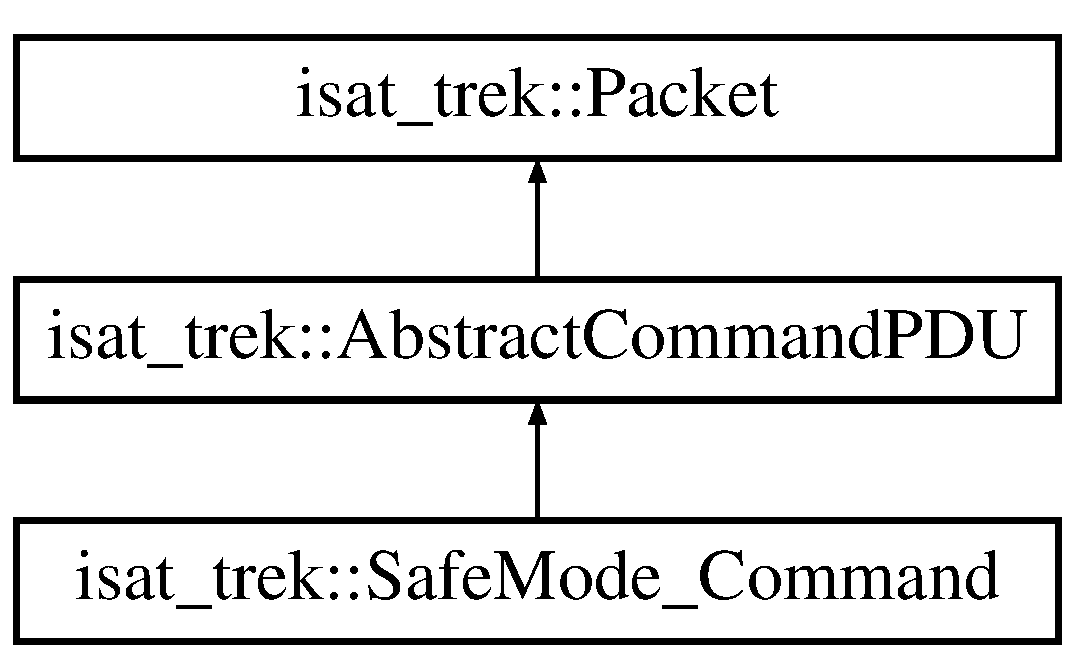
\includegraphics[height=3.000000cm]{classisat__trek_1_1_safe_mode___command}
\end{center}
\end{figure}
\subsection*{Public Member Functions}
\begin{DoxyCompactItemize}
\item 
bool \hyperlink{classisat__trek_1_1_safe_mode___command_a402d7d88e693a73a09323e8fac698a54}{from\+Bytes} (Byte\+Buffer \&buf)
\item 
bool \hyperlink{classisat__trek_1_1_safe_mode___command_ad9688d75bc24e7474eef932cc7dcc180}{to\+Bytes} (Byte\+Buffer \&buf)
\end{DoxyCompactItemize}
\subsection*{Additional Inherited Members}


\subsection{Detailed Description}
X\+XX\+: Replace with real description in isat.\+pdu file. 

\subsection{Member Function Documentation}
\index{isat\+\_\+trek\+::\+Safe\+Mode\+\_\+\+Command@{isat\+\_\+trek\+::\+Safe\+Mode\+\_\+\+Command}!from\+Bytes@{from\+Bytes}}
\index{from\+Bytes@{from\+Bytes}!isat\+\_\+trek\+::\+Safe\+Mode\+\_\+\+Command@{isat\+\_\+trek\+::\+Safe\+Mode\+\_\+\+Command}}
\subsubsection[{\texorpdfstring{from\+Bytes(\+Byte\+Buffer \&buf)}{fromBytes(ByteBuffer &buf)}}]{\setlength{\rightskip}{0pt plus 5cm}bool isat\+\_\+trek\+::\+Safe\+Mode\+\_\+\+Command\+::from\+Bytes (
\begin{DoxyParamCaption}
\item[{Byte\+Buffer \&}]{buf}
\end{DoxyParamCaption}
)\hspace{0.3cm}{\ttfamily [virtual]}}\hypertarget{classisat__trek_1_1_safe_mode___command_a402d7d88e693a73a09323e8fac698a54}{}\label{classisat__trek_1_1_safe_mode___command_a402d7d88e693a73a09323e8fac698a54}
Populate the header and command fields from the data in buf.

\begin{DoxyReturn}{Returns}
true if successful. 
\end{DoxyReturn}


Implements \hyperlink{classisat__trek_1_1_packet}{isat\+\_\+trek\+::\+Packet}.

\index{isat\+\_\+trek\+::\+Safe\+Mode\+\_\+\+Command@{isat\+\_\+trek\+::\+Safe\+Mode\+\_\+\+Command}!to\+Bytes@{to\+Bytes}}
\index{to\+Bytes@{to\+Bytes}!isat\+\_\+trek\+::\+Safe\+Mode\+\_\+\+Command@{isat\+\_\+trek\+::\+Safe\+Mode\+\_\+\+Command}}
\subsubsection[{\texorpdfstring{to\+Bytes(\+Byte\+Buffer \&buf)}{toBytes(ByteBuffer &buf)}}]{\setlength{\rightskip}{0pt plus 5cm}bool isat\+\_\+trek\+::\+Safe\+Mode\+\_\+\+Command\+::to\+Bytes (
\begin{DoxyParamCaption}
\item[{Byte\+Buffer \&}]{buf}
\end{DoxyParamCaption}
)\hspace{0.3cm}{\ttfamily [virtual]}}\hypertarget{classisat__trek_1_1_safe_mode___command_ad9688d75bc24e7474eef932cc7dcc180}{}\label{classisat__trek_1_1_safe_mode___command_ad9688d75bc24e7474eef932cc7dcc180}
Create the binary representation of this instance in the specified buffer.

\begin{DoxyReturn}{Returns}
true if successful. 
\end{DoxyReturn}


Implements \hyperlink{classisat__trek_1_1_packet}{isat\+\_\+trek\+::\+Packet}.



The documentation for this class was generated from the following files\+:\begin{DoxyCompactItemize}
\item 
/home/riley/work/fsw/src/isatgs/\+B\+A\+R\+Co\+Mm\+S/src/dependencies/trek/command/Safe\+Mode\+\_\+\+Command.\+h\item 
/home/riley/work/fsw/src/isatgs/\+B\+A\+R\+Co\+Mm\+S/src/dependencies/trek/command/Safe\+Mode\+\_\+\+Command.\+cpp\end{DoxyCompactItemize}

\hypertarget{classisat__trek_1_1_set_dev_avail___command}{}\section{isat\+\_\+trek\+:\+:Set\+Dev\+Avail\+\_\+\+Command Class Reference}
\label{classisat__trek_1_1_set_dev_avail___command}\index{isat\+\_\+trek\+::\+Set\+Dev\+Avail\+\_\+\+Command@{isat\+\_\+trek\+::\+Set\+Dev\+Avail\+\_\+\+Command}}


{\ttfamily \#include $<$Set\+Dev\+Avail\+\_\+\+Command.\+h$>$}

Inheritance diagram for isat\+\_\+trek\+:\+:Set\+Dev\+Avail\+\_\+\+Command\+:\begin{figure}[H]
\begin{center}
\leavevmode
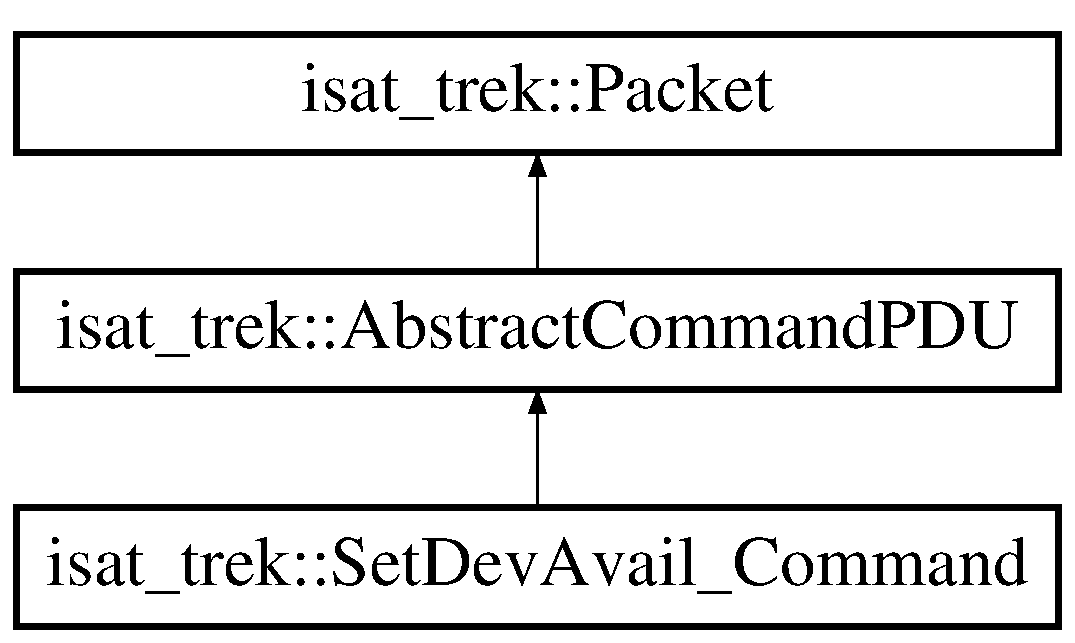
\includegraphics[height=3.000000cm]{classisat__trek_1_1_set_dev_avail___command}
\end{center}
\end{figure}
\subsection*{Public Member Functions}
\begin{DoxyCompactItemize}
\item 
bool \hyperlink{classisat__trek_1_1_set_dev_avail___command_a41c65b9d92d15530c3714523d95f052f}{from\+Bytes} (Byte\+Buffer \&buf)
\item 
bool \hyperlink{classisat__trek_1_1_set_dev_avail___command_a81fdec7886aaa46a16ec318a56f76801}{to\+Bytes} (Byte\+Buffer \&buf)
\end{DoxyCompactItemize}
\subsection*{Public Attributes}
\begin{DoxyCompactItemize}
\item 
int {\bfseries device} = 0\hypertarget{classisat__trek_1_1_set_dev_avail___command_aef0511b825179928d6b3d9784e0bf98f}{}\label{classisat__trek_1_1_set_dev_avail___command_aef0511b825179928d6b3d9784e0bf98f}

\item 
int {\bfseries state} = 0\hypertarget{classisat__trek_1_1_set_dev_avail___command_a385aa636f92971e5d9bd708561e07210}{}\label{classisat__trek_1_1_set_dev_avail___command_a385aa636f92971e5d9bd708561e07210}

\end{DoxyCompactItemize}


\subsection{Detailed Description}
X\+XX\+: Replace with real description in isat.\+pdu file. 

\subsection{Member Function Documentation}
\index{isat\+\_\+trek\+::\+Set\+Dev\+Avail\+\_\+\+Command@{isat\+\_\+trek\+::\+Set\+Dev\+Avail\+\_\+\+Command}!from\+Bytes@{from\+Bytes}}
\index{from\+Bytes@{from\+Bytes}!isat\+\_\+trek\+::\+Set\+Dev\+Avail\+\_\+\+Command@{isat\+\_\+trek\+::\+Set\+Dev\+Avail\+\_\+\+Command}}
\subsubsection[{\texorpdfstring{from\+Bytes(\+Byte\+Buffer \&buf)}{fromBytes(ByteBuffer &buf)}}]{\setlength{\rightskip}{0pt plus 5cm}bool isat\+\_\+trek\+::\+Set\+Dev\+Avail\+\_\+\+Command\+::from\+Bytes (
\begin{DoxyParamCaption}
\item[{Byte\+Buffer \&}]{buf}
\end{DoxyParamCaption}
)\hspace{0.3cm}{\ttfamily [virtual]}}\hypertarget{classisat__trek_1_1_set_dev_avail___command_a41c65b9d92d15530c3714523d95f052f}{}\label{classisat__trek_1_1_set_dev_avail___command_a41c65b9d92d15530c3714523d95f052f}
Populate the header and command fields from the data in buf.

\begin{DoxyReturn}{Returns}
true if successful. 
\end{DoxyReturn}


Implements \hyperlink{classisat__trek_1_1_packet}{isat\+\_\+trek\+::\+Packet}.

\index{isat\+\_\+trek\+::\+Set\+Dev\+Avail\+\_\+\+Command@{isat\+\_\+trek\+::\+Set\+Dev\+Avail\+\_\+\+Command}!to\+Bytes@{to\+Bytes}}
\index{to\+Bytes@{to\+Bytes}!isat\+\_\+trek\+::\+Set\+Dev\+Avail\+\_\+\+Command@{isat\+\_\+trek\+::\+Set\+Dev\+Avail\+\_\+\+Command}}
\subsubsection[{\texorpdfstring{to\+Bytes(\+Byte\+Buffer \&buf)}{toBytes(ByteBuffer &buf)}}]{\setlength{\rightskip}{0pt plus 5cm}bool isat\+\_\+trek\+::\+Set\+Dev\+Avail\+\_\+\+Command\+::to\+Bytes (
\begin{DoxyParamCaption}
\item[{Byte\+Buffer \&}]{buf}
\end{DoxyParamCaption}
)\hspace{0.3cm}{\ttfamily [virtual]}}\hypertarget{classisat__trek_1_1_set_dev_avail___command_a81fdec7886aaa46a16ec318a56f76801}{}\label{classisat__trek_1_1_set_dev_avail___command_a81fdec7886aaa46a16ec318a56f76801}
Create the binary representation of this instance in the specified buffer.

\begin{DoxyReturn}{Returns}
true if successful. 
\end{DoxyReturn}


Implements \hyperlink{classisat__trek_1_1_packet}{isat\+\_\+trek\+::\+Packet}.



The documentation for this class was generated from the following files\+:\begin{DoxyCompactItemize}
\item 
/home/riley/work/fsw/src/isatgs/\+B\+A\+R\+Co\+Mm\+S/src/dependencies/trek/command/Set\+Dev\+Avail\+\_\+\+Command.\+h\item 
/home/riley/work/fsw/src/isatgs/\+B\+A\+R\+Co\+Mm\+S/src/dependencies/trek/command/Set\+Dev\+Avail\+\_\+\+Command.\+cpp\end{DoxyCompactItemize}

\hypertarget{classisat__trek_1_1_set_dev_power___command}{}\section{isat\+\_\+trek\+:\+:Set\+Dev\+Power\+\_\+\+Command Class Reference}
\label{classisat__trek_1_1_set_dev_power___command}\index{isat\+\_\+trek\+::\+Set\+Dev\+Power\+\_\+\+Command@{isat\+\_\+trek\+::\+Set\+Dev\+Power\+\_\+\+Command}}


{\ttfamily \#include $<$Set\+Dev\+Power\+\_\+\+Command.\+h$>$}

Inheritance diagram for isat\+\_\+trek\+:\+:Set\+Dev\+Power\+\_\+\+Command\+:\begin{figure}[H]
\begin{center}
\leavevmode
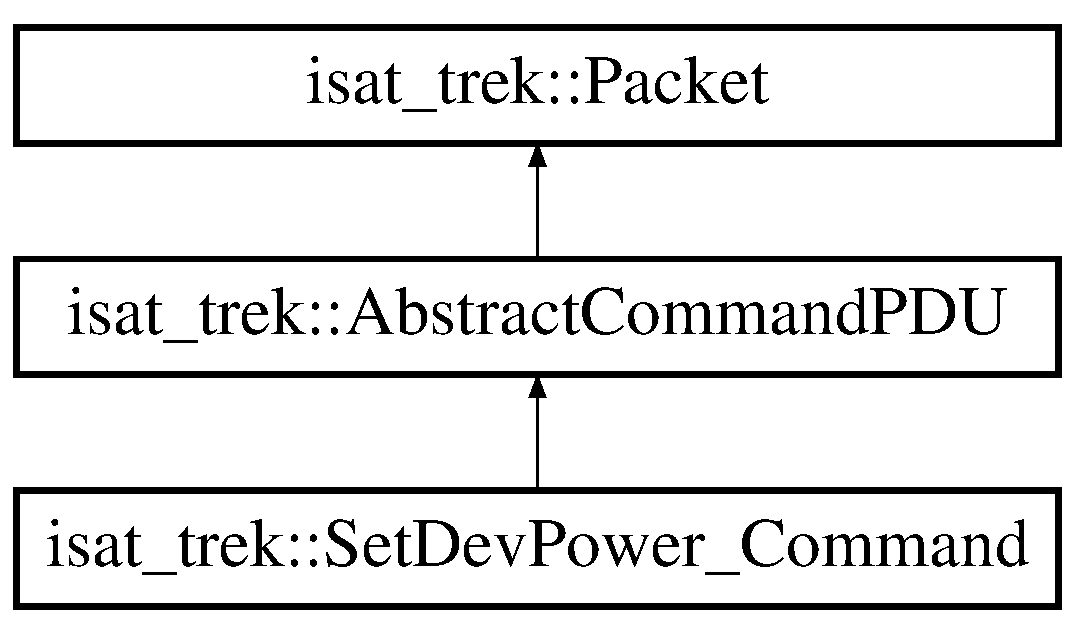
\includegraphics[height=3.000000cm]{classisat__trek_1_1_set_dev_power___command}
\end{center}
\end{figure}
\subsection*{Public Member Functions}
\begin{DoxyCompactItemize}
\item 
bool \hyperlink{classisat__trek_1_1_set_dev_power___command_a4bf3fb3a3f5ae96634935e37182a900e}{from\+Bytes} (Byte\+Buffer \&buf)
\item 
bool \hyperlink{classisat__trek_1_1_set_dev_power___command_a96f838bf99fc8bcaa50f89c4868f1a12}{to\+Bytes} (Byte\+Buffer \&buf)
\end{DoxyCompactItemize}
\subsection*{Public Attributes}
\begin{DoxyCompactItemize}
\item 
int {\bfseries device} = 0\hypertarget{classisat__trek_1_1_set_dev_power___command_a646ab0683c14bea03dd060393b28c950}{}\label{classisat__trek_1_1_set_dev_power___command_a646ab0683c14bea03dd060393b28c950}

\item 
int {\bfseries state} = 0\hypertarget{classisat__trek_1_1_set_dev_power___command_a07c22aedc9cd729659ec313699329129}{}\label{classisat__trek_1_1_set_dev_power___command_a07c22aedc9cd729659ec313699329129}

\end{DoxyCompactItemize}


\subsection{Detailed Description}
X\+XX\+: Replace with real description in isat.\+pdu file. 

\subsection{Member Function Documentation}
\index{isat\+\_\+trek\+::\+Set\+Dev\+Power\+\_\+\+Command@{isat\+\_\+trek\+::\+Set\+Dev\+Power\+\_\+\+Command}!from\+Bytes@{from\+Bytes}}
\index{from\+Bytes@{from\+Bytes}!isat\+\_\+trek\+::\+Set\+Dev\+Power\+\_\+\+Command@{isat\+\_\+trek\+::\+Set\+Dev\+Power\+\_\+\+Command}}
\subsubsection[{\texorpdfstring{from\+Bytes(\+Byte\+Buffer \&buf)}{fromBytes(ByteBuffer &buf)}}]{\setlength{\rightskip}{0pt plus 5cm}bool isat\+\_\+trek\+::\+Set\+Dev\+Power\+\_\+\+Command\+::from\+Bytes (
\begin{DoxyParamCaption}
\item[{Byte\+Buffer \&}]{buf}
\end{DoxyParamCaption}
)\hspace{0.3cm}{\ttfamily [virtual]}}\hypertarget{classisat__trek_1_1_set_dev_power___command_a4bf3fb3a3f5ae96634935e37182a900e}{}\label{classisat__trek_1_1_set_dev_power___command_a4bf3fb3a3f5ae96634935e37182a900e}
Populate the header and command fields from the data in buf.

\begin{DoxyReturn}{Returns}
true if successful. 
\end{DoxyReturn}


Implements \hyperlink{classisat__trek_1_1_packet}{isat\+\_\+trek\+::\+Packet}.

\index{isat\+\_\+trek\+::\+Set\+Dev\+Power\+\_\+\+Command@{isat\+\_\+trek\+::\+Set\+Dev\+Power\+\_\+\+Command}!to\+Bytes@{to\+Bytes}}
\index{to\+Bytes@{to\+Bytes}!isat\+\_\+trek\+::\+Set\+Dev\+Power\+\_\+\+Command@{isat\+\_\+trek\+::\+Set\+Dev\+Power\+\_\+\+Command}}
\subsubsection[{\texorpdfstring{to\+Bytes(\+Byte\+Buffer \&buf)}{toBytes(ByteBuffer &buf)}}]{\setlength{\rightskip}{0pt plus 5cm}bool isat\+\_\+trek\+::\+Set\+Dev\+Power\+\_\+\+Command\+::to\+Bytes (
\begin{DoxyParamCaption}
\item[{Byte\+Buffer \&}]{buf}
\end{DoxyParamCaption}
)\hspace{0.3cm}{\ttfamily [virtual]}}\hypertarget{classisat__trek_1_1_set_dev_power___command_a96f838bf99fc8bcaa50f89c4868f1a12}{}\label{classisat__trek_1_1_set_dev_power___command_a96f838bf99fc8bcaa50f89c4868f1a12}
Create the binary representation of this instance in the specified buffer.

\begin{DoxyReturn}{Returns}
true if successful. 
\end{DoxyReturn}


Implements \hyperlink{classisat__trek_1_1_packet}{isat\+\_\+trek\+::\+Packet}.



The documentation for this class was generated from the following files\+:\begin{DoxyCompactItemize}
\item 
/home/riley/work/fsw/src/isatgs/\+B\+A\+R\+Co\+Mm\+S/src/dependencies/trek/command/Set\+Dev\+Power\+\_\+\+Command.\+h\item 
/home/riley/work/fsw/src/isatgs/\+B\+A\+R\+Co\+Mm\+S/src/dependencies/trek/command/Set\+Dev\+Power\+\_\+\+Command.\+cpp\end{DoxyCompactItemize}

\hypertarget{class_setter}{}\section{Setter Class Reference}
\label{class_setter}\index{Setter@{Setter}}
Inheritance diagram for Setter\+:\begin{figure}[H]
\begin{center}
\leavevmode
\includegraphics[height=2.000000cm]{class_setter}
\end{center}
\end{figure}
\subsection*{Signals}
\begin{DoxyCompactItemize}
\item 
void {\bfseries setter\+\_\+append\+Output} (\hyperlink{struct_m_i_b}{M\+IB} mib)\hypertarget{class_setter_aa3c31dda34bdc33a77ab66ad1923c1cd}{}\label{class_setter_aa3c31dda34bdc33a77ab66ad1923c1cd}

\end{DoxyCompactItemize}
\subsection*{Public Member Functions}
\begin{DoxyCompactItemize}
\item 
{\bfseries Setter} (Q\+Widget $\ast$parent=0)\hypertarget{class_setter_a8d48648f19fb889b72572b529cce86c9}{}\label{class_setter_a8d48648f19fb889b72572b529cce86c9}

\item 
void {\bfseries setter\+\_\+change\+Load\+Vals} ()\hypertarget{class_setter_a16f30bad63779adfe155156f31a7ca3a}{}\label{class_setter_a16f30bad63779adfe155156f31a7ca3a}

\end{DoxyCompactItemize}


The documentation for this class was generated from the following files\+:\begin{DoxyCompactItemize}
\item 
/home/riley/work/fsw/src/isatgs/\+B\+A\+R\+Co\+Mm\+S/src/modules/\+B\+A\+R\+Co\+Mm\+S\+\_\+\+C\+F\+D\+P/setter.\+h\item 
/home/riley/work/fsw/src/isatgs/\+B\+A\+R\+Co\+Mm\+S/src/modules/\+B\+A\+R\+Co\+Mm\+S\+\_\+\+C\+F\+D\+P/setter.\+cpp\end{DoxyCompactItemize}

\hypertarget{class_sim}{}\section{Sim Class Reference}
\label{class_sim}\index{Sim@{Sim}}
Inheritance diagram for Sim\+:\begin{figure}[H]
\begin{center}
\leavevmode
\includegraphics[height=2.000000cm]{class_sim}
\end{center}
\end{figure}
\subsection*{Signals}
\begin{DoxyCompactItemize}
\item 
void {\bfseries sim\+\_\+append\+Output} (\hyperlink{struct_link_sim}{Link\+Sim} sim)\hypertarget{class_sim_afc12f2f23c51332f4feaa7b5e0ea461f}{}\label{class_sim_afc12f2f23c51332f4feaa7b5e0ea461f}

\end{DoxyCompactItemize}
\subsection*{Public Member Functions}
\begin{DoxyCompactItemize}
\item 
{\bfseries Sim} (Q\+Widget $\ast$parent=0)\hypertarget{class_sim_ae84d420452fc950c0a0bfe523e1c030d}{}\label{class_sim_ae84d420452fc950c0a0bfe523e1c030d}

\item 
void {\bfseries sim\+\_\+change\+Load\+Vals} ()\hypertarget{class_sim_a8a8d0fa162b1eb548a0c97055d1ea124}{}\label{class_sim_a8a8d0fa162b1eb548a0c97055d1ea124}

\end{DoxyCompactItemize}


The documentation for this class was generated from the following files\+:\begin{DoxyCompactItemize}
\item 
/home/riley/work/fsw/src/isatgs/\+B\+A\+R\+Co\+Mm\+S/src/modules/\+B\+A\+R\+Co\+Mm\+S\+\_\+\+C\+F\+D\+P/sim.\+h\item 
/home/riley/work/fsw/src/isatgs/\+B\+A\+R\+Co\+Mm\+S/src/modules/\+B\+A\+R\+Co\+Mm\+S\+\_\+\+C\+F\+D\+P/sim.\+cpp\end{DoxyCompactItemize}

\hypertarget{classisat__utils_1_1_simple_mutex_lock}{}\section{isat\+\_\+utils\+:\+:Simple\+Mutex\+Lock Class Reference}
\label{classisat__utils_1_1_simple_mutex_lock}\index{isat\+\_\+utils\+::\+Simple\+Mutex\+Lock@{isat\+\_\+utils\+::\+Simple\+Mutex\+Lock}}
\subsection*{Public Member Functions}
\begin{DoxyCompactItemize}
\item 
{\bfseries Simple\+Mutex\+Lock} (pthread\+\_\+mutex\+\_\+t $\ast$mutex)\hypertarget{classisat__utils_1_1_simple_mutex_lock_a7590d3ad64870694d9b5cb0396d00568}{}\label{classisat__utils_1_1_simple_mutex_lock_a7590d3ad64870694d9b5cb0396d00568}

\end{DoxyCompactItemize}
\subsection*{Protected Attributes}
\begin{DoxyCompactItemize}
\item 
pthread\+\_\+mutex\+\_\+t $\ast$ {\bfseries my\+Mutex}\hypertarget{classisat__utils_1_1_simple_mutex_lock_a12360895886a2dc13d015e7eeb978c29}{}\label{classisat__utils_1_1_simple_mutex_lock_a12360895886a2dc13d015e7eeb978c29}

\end{DoxyCompactItemize}


The documentation for this class was generated from the following files\+:\begin{DoxyCompactItemize}
\item 
/home/riley/work/fsw/src/isatgs/\+B\+A\+R\+Co\+Mm\+S/src/dependencies/utils/Simple\+Mutex\+Lock.\+h\item 
/home/riley/work/fsw/src/isatgs/\+B\+A\+R\+Co\+Mm\+S/src/dependencies/utils/Simple\+Mutex\+Lock.\+cpp\end{DoxyCompactItemize}

\hypertarget{structsort_by_command}{}\section{sort\+By\+Command Struct Reference}
\label{structsort_by_command}\index{sort\+By\+Command@{sort\+By\+Command}}
\subsection*{Public Member Functions}
\begin{DoxyCompactItemize}
\item 
bool {\bfseries operator()} (\hyperlink{class_f_s_w_item}{F\+S\+W\+Item} $\ast$start, \hyperlink{class_f_s_w_item}{F\+S\+W\+Item} $\ast$end)\hypertarget{structsort_by_command_a87753a83cf6532564f1f849e7da20edb}{}\label{structsort_by_command_a87753a83cf6532564f1f849e7da20edb}

\end{DoxyCompactItemize}


The documentation for this struct was generated from the following file\+:\begin{DoxyCompactItemize}
\item 
/home/riley/work/fsw/src/isatgs/\+B\+A\+R\+Co\+Mm\+S/src/modules/\+B\+A\+R\+Co\+Mm\+S\+\_\+\+Bulletin/fswitem.\+h\end{DoxyCompactItemize}

\hypertarget{structsort_by_command2}{}\section{sort\+By\+Command2 Struct Reference}
\label{structsort_by_command2}\index{sort\+By\+Command2@{sort\+By\+Command2}}
\subsection*{Public Member Functions}
\begin{DoxyCompactItemize}
\item 
bool {\bfseries operator()} (\hyperlink{class_f_s_w_item}{F\+S\+W\+Item} $\ast$start, \hyperlink{class_f_s_w_item}{F\+S\+W\+Item} $\ast$end)\hypertarget{structsort_by_command2_af15ad4b3511161b525f8efdd33f07b3f}{}\label{structsort_by_command2_af15ad4b3511161b525f8efdd33f07b3f}

\end{DoxyCompactItemize}


The documentation for this struct was generated from the following file\+:\begin{DoxyCompactItemize}
\item 
/home/riley/work/fsw/src/isatgs/\+B\+A\+R\+Co\+Mm\+S/src/modules/\+B\+A\+R\+Co\+Mm\+S\+\_\+\+Bulletin/fswitem.\+h\end{DoxyCompactItemize}

\hypertarget{structsort_by_size}{}\section{sort\+By\+Size Struct Reference}
\label{structsort_by_size}\index{sort\+By\+Size@{sort\+By\+Size}}
\subsection*{Public Member Functions}
\begin{DoxyCompactItemize}
\item 
bool {\bfseries operator()} (const \hyperlink{class_item}{Item} \&start, const \hyperlink{class_item}{Item} \&end)\hypertarget{structsort_by_size_aafa71dce1e956d3c36ed6b42b7167ffb}{}\label{structsort_by_size_aafa71dce1e956d3c36ed6b42b7167ffb}

\end{DoxyCompactItemize}


The documentation for this struct was generated from the following file\+:\begin{DoxyCompactItemize}
\item 
/home/riley/work/fsw/src/isatgs/\+B\+A\+R\+Co\+Mm\+S/src/modules/\+B\+A\+R\+Co\+Mm\+S\+\_\+\+Bulletin/item.\+h\end{DoxyCompactItemize}

\hypertarget{structsort_by_size2}{}\section{sort\+By\+Size2 Struct Reference}
\label{structsort_by_size2}\index{sort\+By\+Size2@{sort\+By\+Size2}}
\subsection*{Public Member Functions}
\begin{DoxyCompactItemize}
\item 
bool {\bfseries operator()} (const \hyperlink{class_item}{Item} \&start, const \hyperlink{class_item}{Item} \&end)\hypertarget{structsort_by_size2_ae81846c497c001b7a155a4497b221859}{}\label{structsort_by_size2_ae81846c497c001b7a155a4497b221859}

\end{DoxyCompactItemize}


The documentation for this struct was generated from the following file\+:\begin{DoxyCompactItemize}
\item 
/home/riley/work/fsw/src/isatgs/\+B\+A\+R\+Co\+Mm\+S/src/modules/\+B\+A\+R\+Co\+Mm\+S\+\_\+\+Bulletin/item.\+h\end{DoxyCompactItemize}

\hypertarget{structsort_by_status_c_f_d_p}{}\section{sort\+By\+Status\+C\+F\+DP Struct Reference}
\label{structsort_by_status_c_f_d_p}\index{sort\+By\+Status\+C\+F\+DP@{sort\+By\+Status\+C\+F\+DP}}
\subsection*{Public Member Functions}
\begin{DoxyCompactItemize}
\item 
bool {\bfseries operator()} (const \hyperlink{class_item}{Item} \&start, const \hyperlink{class_item}{Item} \&end)\hypertarget{structsort_by_status_c_f_d_p_a5afef599c86111f373c40bdf8fb9f236}{}\label{structsort_by_status_c_f_d_p_a5afef599c86111f373c40bdf8fb9f236}

\end{DoxyCompactItemize}


The documentation for this struct was generated from the following file\+:\begin{DoxyCompactItemize}
\item 
/home/riley/work/fsw/src/isatgs/\+B\+A\+R\+Co\+Mm\+S/src/modules/\+B\+A\+R\+Co\+Mm\+S\+\_\+\+Bulletin/item.\+h\end{DoxyCompactItemize}

\hypertarget{structsort_by_status_c_f_d_p2}{}\section{sort\+By\+Status\+C\+F\+D\+P2 Struct Reference}
\label{structsort_by_status_c_f_d_p2}\index{sort\+By\+Status\+C\+F\+D\+P2@{sort\+By\+Status\+C\+F\+D\+P2}}
\subsection*{Public Member Functions}
\begin{DoxyCompactItemize}
\item 
bool {\bfseries operator()} (const \hyperlink{class_item}{Item} \&start, const \hyperlink{class_item}{Item} \&end)\hypertarget{structsort_by_status_c_f_d_p2_ab4bd1e199a982b6cc924a9fe916095f4}{}\label{structsort_by_status_c_f_d_p2_ab4bd1e199a982b6cc924a9fe916095f4}

\end{DoxyCompactItemize}


The documentation for this struct was generated from the following file\+:\begin{DoxyCompactItemize}
\item 
/home/riley/work/fsw/src/isatgs/\+B\+A\+R\+Co\+Mm\+S/src/modules/\+B\+A\+R\+Co\+Mm\+S\+\_\+\+Bulletin/item.\+h\end{DoxyCompactItemize}

\hypertarget{structsort_by_status_f_s_w}{}\section{sort\+By\+Status\+F\+SW Struct Reference}
\label{structsort_by_status_f_s_w}\index{sort\+By\+Status\+F\+SW@{sort\+By\+Status\+F\+SW}}
\subsection*{Public Member Functions}
\begin{DoxyCompactItemize}
\item 
bool {\bfseries operator()} (\hyperlink{class_f_s_w_item}{F\+S\+W\+Item} $\ast$start, \hyperlink{class_f_s_w_item}{F\+S\+W\+Item} $\ast$end)\hypertarget{structsort_by_status_f_s_w_a57a6cfebace4e22c183fd24ec3cc75d7}{}\label{structsort_by_status_f_s_w_a57a6cfebace4e22c183fd24ec3cc75d7}

\end{DoxyCompactItemize}


The documentation for this struct was generated from the following file\+:\begin{DoxyCompactItemize}
\item 
/home/riley/work/fsw/src/isatgs/\+B\+A\+R\+Co\+Mm\+S/src/modules/\+B\+A\+R\+Co\+Mm\+S\+\_\+\+Bulletin/fswitem.\+h\end{DoxyCompactItemize}

\hypertarget{structsort_by_status_f_s_w2}{}\section{sort\+By\+Status\+F\+S\+W2 Struct Reference}
\label{structsort_by_status_f_s_w2}\index{sort\+By\+Status\+F\+S\+W2@{sort\+By\+Status\+F\+S\+W2}}
\subsection*{Public Member Functions}
\begin{DoxyCompactItemize}
\item 
bool {\bfseries operator()} (\hyperlink{class_f_s_w_item}{F\+S\+W\+Item} $\ast$start, \hyperlink{class_f_s_w_item}{F\+S\+W\+Item} $\ast$end)\hypertarget{structsort_by_status_f_s_w2_a83f2251fe6e6f3cf6d791a1cb46a611d}{}\label{structsort_by_status_f_s_w2_a83f2251fe6e6f3cf6d791a1cb46a611d}

\end{DoxyCompactItemize}


The documentation for this struct was generated from the following file\+:\begin{DoxyCompactItemize}
\item 
/home/riley/work/fsw/src/isatgs/\+B\+A\+R\+Co\+Mm\+S/src/modules/\+B\+A\+R\+Co\+Mm\+S\+\_\+\+Bulletin/fswitem.\+h\end{DoxyCompactItemize}

\hypertarget{structsort_by_time_c_f_d_p}{}\section{sort\+By\+Time\+C\+F\+DP Struct Reference}
\label{structsort_by_time_c_f_d_p}\index{sort\+By\+Time\+C\+F\+DP@{sort\+By\+Time\+C\+F\+DP}}
\subsection*{Public Member Functions}
\begin{DoxyCompactItemize}
\item 
bool {\bfseries operator()} (const \hyperlink{class_item}{Item} \&start, const \hyperlink{class_item}{Item} \&end)\hypertarget{structsort_by_time_c_f_d_p_a12a01dc63586c113d86bb673d720627b}{}\label{structsort_by_time_c_f_d_p_a12a01dc63586c113d86bb673d720627b}

\end{DoxyCompactItemize}


The documentation for this struct was generated from the following file\+:\begin{DoxyCompactItemize}
\item 
/home/riley/work/fsw/src/isatgs/\+B\+A\+R\+Co\+Mm\+S/src/modules/\+B\+A\+R\+Co\+Mm\+S\+\_\+\+Bulletin/item.\+h\end{DoxyCompactItemize}

\hypertarget{structsort_by_time_c_f_d_p2}{}\section{sort\+By\+Time\+C\+F\+D\+P2 Struct Reference}
\label{structsort_by_time_c_f_d_p2}\index{sort\+By\+Time\+C\+F\+D\+P2@{sort\+By\+Time\+C\+F\+D\+P2}}
\subsection*{Public Member Functions}
\begin{DoxyCompactItemize}
\item 
bool {\bfseries operator()} (const \hyperlink{class_item}{Item} \&start, const \hyperlink{class_item}{Item} \&end)\hypertarget{structsort_by_time_c_f_d_p2_a8a53b8e3f6621e8c224bb82c84435def}{}\label{structsort_by_time_c_f_d_p2_a8a53b8e3f6621e8c224bb82c84435def}

\end{DoxyCompactItemize}


The documentation for this struct was generated from the following file\+:\begin{DoxyCompactItemize}
\item 
/home/riley/work/fsw/src/isatgs/\+B\+A\+R\+Co\+Mm\+S/src/modules/\+B\+A\+R\+Co\+Mm\+S\+\_\+\+Bulletin/item.\+h\end{DoxyCompactItemize}

\hypertarget{structsort_by_time_f_s_w}{}\section{sort\+By\+Time\+F\+SW Struct Reference}
\label{structsort_by_time_f_s_w}\index{sort\+By\+Time\+F\+SW@{sort\+By\+Time\+F\+SW}}
\subsection*{Public Slots}
\begin{DoxyCompactItemize}
\item 
bool {\bfseries operator()} (\hyperlink{class_f_s_w_item}{F\+S\+W\+Item} $\ast$start, \hyperlink{class_f_s_w_item}{F\+S\+W\+Item} $\ast$end)\hypertarget{structsort_by_time_f_s_w_a70093a9584f37dc50b4ce09ef02190f9}{}\label{structsort_by_time_f_s_w_a70093a9584f37dc50b4ce09ef02190f9}

\end{DoxyCompactItemize}


The documentation for this struct was generated from the following file\+:\begin{DoxyCompactItemize}
\item 
/home/riley/work/fsw/src/isatgs/\+B\+A\+R\+Co\+Mm\+S/src/modules/\+B\+A\+R\+Co\+Mm\+S\+\_\+\+Bulletin/fswitem.\+h\end{DoxyCompactItemize}

\hypertarget{structsort_by_time_f_s_w2}{}\section{sort\+By\+Time\+F\+S\+W2 Struct Reference}
\label{structsort_by_time_f_s_w2}\index{sort\+By\+Time\+F\+S\+W2@{sort\+By\+Time\+F\+S\+W2}}
\subsection*{Public Member Functions}
\begin{DoxyCompactItemize}
\item 
bool {\bfseries operator()} (\hyperlink{class_f_s_w_item}{F\+S\+W\+Item} $\ast$start, \hyperlink{class_f_s_w_item}{F\+S\+W\+Item} $\ast$end)\hypertarget{structsort_by_time_f_s_w2_a1d236f3f61e7a10b8de3d272152abbff}{}\label{structsort_by_time_f_s_w2_a1d236f3f61e7a10b8de3d272152abbff}

\end{DoxyCompactItemize}


The documentation for this struct was generated from the following file\+:\begin{DoxyCompactItemize}
\item 
/home/riley/work/fsw/src/isatgs/\+B\+A\+R\+Co\+Mm\+S/src/modules/\+B\+A\+R\+Co\+Mm\+S\+\_\+\+Bulletin/fswitem.\+h\end{DoxyCompactItemize}

\hypertarget{class_sorting}{}\section{Sorting Class Reference}
\label{class_sorting}\index{Sorting@{Sorting}}
Inheritance diagram for Sorting\+:\begin{figure}[H]
\begin{center}
\leavevmode
\includegraphics[height=2.000000cm]{class_sorting}
\end{center}
\end{figure}
\subsection*{Public Slots}
\begin{DoxyCompactItemize}
\item 
void {\bfseries time} ()\hypertarget{class_sorting_af8aa0115ea559d7adde8c7aa94fc837c}{}\label{class_sorting_af8aa0115ea559d7adde8c7aa94fc837c}

\item 
void {\bfseries time2} ()\hypertarget{class_sorting_a0b1cc019829b5d2602cb994f1d9fc999}{}\label{class_sorting_a0b1cc019829b5d2602cb994f1d9fc999}

\item 
void {\bfseries size} ()\hypertarget{class_sorting_a535989339097fe845468fd8aee18d8ad}{}\label{class_sorting_a535989339097fe845468fd8aee18d8ad}

\item 
void {\bfseries size2} ()\hypertarget{class_sorting_acd7b27aab2a5ff7ccbf975402dd3719b}{}\label{class_sorting_acd7b27aab2a5ff7ccbf975402dd3719b}

\item 
void {\bfseries command} ()\hypertarget{class_sorting_ad60f899f4912d268e58fb7abc301a2a3}{}\label{class_sorting_ad60f899f4912d268e58fb7abc301a2a3}

\item 
void {\bfseries command2} ()\hypertarget{class_sorting_a4ec902e66832850acbe37d24aa858457}{}\label{class_sorting_a4ec902e66832850acbe37d24aa858457}

\item 
void {\bfseries status} ()\hypertarget{class_sorting_aeac6672a985d3add82a595f45775897b}{}\label{class_sorting_aeac6672a985d3add82a595f45775897b}

\item 
void {\bfseries status2} ()\hypertarget{class_sorting_af640e0213df2a2d937a3d78e1553a1d8}{}\label{class_sorting_af640e0213df2a2d937a3d78e1553a1d8}

\end{DoxyCompactItemize}
\subsection*{Signals}
\begin{DoxyCompactItemize}
\item 
void {\bfseries chosen} (int sort\+Option)\hypertarget{class_sorting_ac5b16d5fb341031cd0a5c147729d9602}{}\label{class_sorting_ac5b16d5fb341031cd0a5c147729d9602}

\end{DoxyCompactItemize}
\subsection*{Public Member Functions}
\begin{DoxyCompactItemize}
\item 
{\bfseries Sorting} (Q\+Widget $\ast$parent=0)\hypertarget{class_sorting_a2612d18eb93b6c7fbf481ce574763f11}{}\label{class_sorting_a2612d18eb93b6c7fbf481ce574763f11}

\end{DoxyCompactItemize}


The documentation for this class was generated from the following files\+:\begin{DoxyCompactItemize}
\item 
/home/riley/work/fsw/src/isatgs/\+B\+A\+R\+Co\+Mm\+S/src/modules/\+B\+A\+R\+Co\+Mm\+S\+\_\+\+Bulletin/sorting.\+h\item 
/home/riley/work/fsw/src/isatgs/\+B\+A\+R\+Co\+Mm\+S/src/modules/\+B\+A\+R\+Co\+Mm\+S\+\_\+\+Bulletin/sorting.\+cpp\end{DoxyCompactItemize}

\hypertarget{classisat__utils_1_1_string}{}\section{isat\+\_\+utils\+:\+:String Class Reference}
\label{classisat__utils_1_1_string}\index{isat\+\_\+utils\+::\+String@{isat\+\_\+utils\+::\+String}}


{\ttfamily \#include $<$String.\+h$>$}

\subsection*{Public Member Functions}
\begin{DoxyCompactItemize}
\item 
\hyperlink{classisat__utils_1_1_string_a016361e98c3ebbc6b6df8137c38077c1}{String} ()
\item 
\hyperlink{classisat__utils_1_1_string_a3f219032bba25fc4c499abb963badb9f}{String} (char const $\ast$charstring)
\item 
\hyperlink{classisat__utils_1_1_string_a6c36434fa43495939a12eab3e5421081}{String} (\hyperlink{classisat__utils_1_1_string}{String} const \&rhs)
\item 
\hyperlink{classisat__utils_1_1_string}{String} \& \hyperlink{classisat__utils_1_1_string_a49c95362b94c3b62d3f6765105c7a7ba}{operator=} (\hyperlink{classisat__utils_1_1_string}{String} rhs)
\item 
\hyperlink{classisat__utils_1_1_string}{String} \& {\bfseries operator+=} (\hyperlink{classisat__utils_1_1_string}{String} rhs)\hypertarget{classisat__utils_1_1_string_a6f91ae8be5b77eb7697f111198c0fa6c}{}\label{classisat__utils_1_1_string_a6f91ae8be5b77eb7697f111198c0fa6c}

\item 
bool \hyperlink{classisat__utils_1_1_string_a44073c5213f18e79e2a78e32665e5a35}{operator==} (\hyperlink{classisat__utils_1_1_string}{String} rhs)
\item 
bool {\bfseries operator!=} (\hyperlink{classisat__utils_1_1_string}{String} rhs)\hypertarget{classisat__utils_1_1_string_a040e21b8c7f6befc168c6561406f2164}{}\label{classisat__utils_1_1_string_a040e21b8c7f6befc168c6561406f2164}

\item 
bool {\bfseries operator$<$} (\hyperlink{classisat__utils_1_1_string}{String} rhs)\hypertarget{classisat__utils_1_1_string_a89b85a69bde172d3b30c7373a86527ae}{}\label{classisat__utils_1_1_string_a89b85a69bde172d3b30c7373a86527ae}

\item 
bool {\bfseries operator$>$} (\hyperlink{classisat__utils_1_1_string}{String} rhs)\hypertarget{classisat__utils_1_1_string_a7c30434daf5b2c1210f68d4058249d1e}{}\label{classisat__utils_1_1_string_a7c30434daf5b2c1210f68d4058249d1e}

\item 
int \hyperlink{classisat__utils_1_1_string_aebbe51bc0a66580e6fae5a8df6e8197d}{length} () const 
\item 
int \hyperlink{classisat__utils_1_1_string_ace3e7442c0f491e40a3d2591a9f23032}{capacity} () const 
\item 
void \hyperlink{classisat__utils_1_1_string_a63c3cd6bb9e714631bd8c6220a114f21}{clear} ()
\item 
char const $\ast$ \hyperlink{classisat__utils_1_1_string_adb9a310b21d6ae57c5a4402343f55af1}{c\+\_\+str} () const 
\item 
bool \hyperlink{classisat__utils_1_1_string_a8a62556f24cc9bee02190b36166fccae}{char\+At} (int index, char \&c)
\item 
\hyperlink{classisat__utils_1_1_string}{String} {\bfseries substring} (int startpos, int \hyperlink{classisat__utils_1_1_string_aebbe51bc0a66580e6fae5a8df6e8197d}{length})\hypertarget{classisat__utils_1_1_string_af0323aab236cf048cfbd141adaab2606}{}\label{classisat__utils_1_1_string_af0323aab236cf048cfbd141adaab2606}

\item 
\hyperlink{classisat__utils_1_1_string}{String} \hyperlink{classisat__utils_1_1_string_a895148a2d7201b1e45ed863ada35ed0d}{to\+Lower} () const 
\item 
\hyperlink{classisat__utils_1_1_string}{String} \hyperlink{classisat__utils_1_1_string_a3995ede4119f8b094cdb4ffdf73d7e59}{to\+Upper} () const 
\item 
bool {\bfseries parse\+Int} (long \&value)\hypertarget{classisat__utils_1_1_string_a28f610edff258863dc1a5a2c396aab4d}{}\label{classisat__utils_1_1_string_a28f610edff258863dc1a5a2c396aab4d}

\item 
bool {\bfseries parse\+Double} (double \&value)\hypertarget{classisat__utils_1_1_string_a402816d16b35457fdbee9c6ac3390e6b}{}\label{classisat__utils_1_1_string_a402816d16b35457fdbee9c6ac3390e6b}

\item 
bool {\bfseries parse\+Bool} (bool \&value)\hypertarget{classisat__utils_1_1_string_a3dae7076e632c06f368ebf135bf7face}{}\label{classisat__utils_1_1_string_a3dae7076e632c06f368ebf135bf7face}

\item 
bool {\bfseries parse\+Hex} (long \&value)\hypertarget{classisat__utils_1_1_string_ad18ef87cc71dbb4e5b84f7ba5dc8c03a}{}\label{classisat__utils_1_1_string_ad18ef87cc71dbb4e5b84f7ba5dc8c03a}

\item 
bool \hyperlink{classisat__utils_1_1_string_a13d1ca3a639362ddc294de879a0345fa}{matches} (\hyperlink{classisat__utils_1_1_string}{String} regex) const 
\item 
\hyperlink{classisat__utils_1_1_array_list}{Array\+List}$<$ \hyperlink{classisat__utils_1_1_string}{String} $>$ {\bfseries split} (\hyperlink{classisat__utils_1_1_string}{String} regex) const \hypertarget{classisat__utils_1_1_string_a632bc227a1d158e511f1d2abf52f6bc2}{}\label{classisat__utils_1_1_string_a632bc227a1d158e511f1d2abf52f6bc2}

\item 
\hyperlink{classisat__utils_1_1_string_a4c903ee6fadb521dac0d4ff2686c3384}{$\sim$\+String} ()
\item 
bool \hyperlink{classisat__utils_1_1_string_a6cc57bb76f496f68ed9f4e2d0d19514b}{error} () const 
\end{DoxyCompactItemize}
\subsection*{Static Public Member Functions}
\begin{DoxyCompactItemize}
\item 
static \hyperlink{classisat__utils_1_1_string}{String} {\bfseries format} (\hyperlink{classisat__utils_1_1_string}{String} format\+String, int val)\hypertarget{classisat__utils_1_1_string_ac31a5a9fbcbbc2b90a71332fb550ba27}{}\label{classisat__utils_1_1_string_ac31a5a9fbcbbc2b90a71332fb550ba27}

\item 
static \hyperlink{classisat__utils_1_1_string}{String} {\bfseries format} (\hyperlink{classisat__utils_1_1_string}{String} format\+String, float val)\hypertarget{classisat__utils_1_1_string_a8b7108ef6f8c8a5226d858dc79dfc8bd}{}\label{classisat__utils_1_1_string_a8b7108ef6f8c8a5226d858dc79dfc8bd}

\item 
static \hyperlink{classisat__utils_1_1_string}{String} {\bfseries format} (\hyperlink{classisat__utils_1_1_string}{String} format\+String, double val)\hypertarget{classisat__utils_1_1_string_a5147fa966d10e0e07344becb2a3dd62d}{}\label{classisat__utils_1_1_string_a5147fa966d10e0e07344becb2a3dd62d}

\end{DoxyCompactItemize}
\subsection*{Friends}
\begin{DoxyCompactItemize}
\item 
ostream \& {\bfseries operator$<$$<$} (ostream \&ostr, \hyperlink{classisat__utils_1_1_string}{String} const \&str)\hypertarget{classisat__utils_1_1_string_ad2ff8448e2de2f974409f5f07a8f573e}{}\label{classisat__utils_1_1_string_ad2ff8448e2de2f974409f5f07a8f573e}

\item 
\hyperlink{classisat__utils_1_1_string}{String} {\bfseries operator+} (\hyperlink{classisat__utils_1_1_string}{String} a, \hyperlink{classisat__utils_1_1_string}{String} b)\hypertarget{classisat__utils_1_1_string_a2c096e418f6306df9220fd3aefb3e84e}{}\label{classisat__utils_1_1_string_a2c096e418f6306df9220fd3aefb3e84e}

\end{DoxyCompactItemize}


\subsection{Detailed Description}
This class provides a basic string class.

We\textquotesingle{}re not using S\+TL or boost because of the ban on exceptions. This class provides a string class which provides modern string like behavior\+: Dynamic allocated memory, regular expressions, operations on strings, conversion to and from char$\ast$, etc. Not perfect, but better than chasing char$\ast$ all over the place.

X\+XX\+: Modify this class to resize. \hyperlink{classisat__utils_1_1_file}{File} needs it and it\textquotesingle{}s just dumb not to. --jamie 

\subsection{Constructor \& Destructor Documentation}
\index{isat\+\_\+utils\+::\+String@{isat\+\_\+utils\+::\+String}!String@{String}}
\index{String@{String}!isat\+\_\+utils\+::\+String@{isat\+\_\+utils\+::\+String}}
\subsubsection[{\texorpdfstring{String()}{String()}}]{\setlength{\rightskip}{0pt plus 5cm}isat\+\_\+utils\+::\+String\+::\+String (
\begin{DoxyParamCaption}
{}
\end{DoxyParamCaption}
)}\hypertarget{classisat__utils_1_1_string_a016361e98c3ebbc6b6df8137c38077c1}{}\label{classisat__utils_1_1_string_a016361e98c3ebbc6b6df8137c38077c1}
Default constructor. \index{isat\+\_\+utils\+::\+String@{isat\+\_\+utils\+::\+String}!String@{String}}
\index{String@{String}!isat\+\_\+utils\+::\+String@{isat\+\_\+utils\+::\+String}}
\subsubsection[{\texorpdfstring{String(char const $\ast$charstring)}{String(char const *charstring)}}]{\setlength{\rightskip}{0pt plus 5cm}isat\+\_\+utils\+::\+String\+::\+String (
\begin{DoxyParamCaption}
\item[{char const $\ast$}]{charstring}
\end{DoxyParamCaption}
)}\hypertarget{classisat__utils_1_1_string_a3f219032bba25fc4c499abb963badb9f}{}\label{classisat__utils_1_1_string_a3f219032bba25fc4c499abb963badb9f}
Construct a \hyperlink{classisat__utils_1_1_string}{String} instance and initialize from the specified null terminated char$\ast$ string. \index{isat\+\_\+utils\+::\+String@{isat\+\_\+utils\+::\+String}!String@{String}}
\index{String@{String}!isat\+\_\+utils\+::\+String@{isat\+\_\+utils\+::\+String}}
\subsubsection[{\texorpdfstring{String(\+String const \&rhs)}{String(String const &rhs)}}]{\setlength{\rightskip}{0pt plus 5cm}isat\+\_\+utils\+::\+String\+::\+String (
\begin{DoxyParamCaption}
\item[{{\bf String} const \&}]{rhs}
\end{DoxyParamCaption}
)}\hypertarget{classisat__utils_1_1_string_a6c36434fa43495939a12eab3e5421081}{}\label{classisat__utils_1_1_string_a6c36434fa43495939a12eab3e5421081}
Copy constructor. \index{isat\+\_\+utils\+::\+String@{isat\+\_\+utils\+::\+String}!````~String@{$\sim$\+String}}
\index{````~String@{$\sim$\+String}!isat\+\_\+utils\+::\+String@{isat\+\_\+utils\+::\+String}}
\subsubsection[{\texorpdfstring{$\sim$\+String()}{~String()}}]{\setlength{\rightskip}{0pt plus 5cm}isat\+\_\+utils\+::\+String\+::$\sim$\+String (
\begin{DoxyParamCaption}
{}
\end{DoxyParamCaption}
)}\hypertarget{classisat__utils_1_1_string_a4c903ee6fadb521dac0d4ff2686c3384}{}\label{classisat__utils_1_1_string_a4c903ee6fadb521dac0d4ff2686c3384}
Destructor. 

\subsection{Member Function Documentation}
\index{isat\+\_\+utils\+::\+String@{isat\+\_\+utils\+::\+String}!c\+\_\+str@{c\+\_\+str}}
\index{c\+\_\+str@{c\+\_\+str}!isat\+\_\+utils\+::\+String@{isat\+\_\+utils\+::\+String}}
\subsubsection[{\texorpdfstring{c\+\_\+str() const }{c_str() const }}]{\setlength{\rightskip}{0pt plus 5cm}char const $\ast$ isat\+\_\+utils\+::\+String\+::c\+\_\+str (
\begin{DoxyParamCaption}
{}
\end{DoxyParamCaption}
) const}\hypertarget{classisat__utils_1_1_string_adb9a310b21d6ae57c5a4402343f55af1}{}\label{classisat__utils_1_1_string_adb9a310b21d6ae57c5a4402343f55af1}
Access the null terminated \textquotesingle{}C\textquotesingle{} string representation of this instance.

\begin{DoxyReturn}{Returns}
A pointed to the null terminated C string encapsulated by this \hyperlink{classisat__utils_1_1_string}{String} instance. 
\end{DoxyReturn}
\index{isat\+\_\+utils\+::\+String@{isat\+\_\+utils\+::\+String}!capacity@{capacity}}
\index{capacity@{capacity}!isat\+\_\+utils\+::\+String@{isat\+\_\+utils\+::\+String}}
\subsubsection[{\texorpdfstring{capacity() const }{capacity() const }}]{\setlength{\rightskip}{0pt plus 5cm}int isat\+\_\+utils\+::\+String\+::capacity (
\begin{DoxyParamCaption}
{}
\end{DoxyParamCaption}
) const}\hypertarget{classisat__utils_1_1_string_ace3e7442c0f491e40a3d2591a9f23032}{}\label{classisat__utils_1_1_string_ace3e7442c0f491e40a3d2591a9f23032}
The capacity is the maximum number of characters that can be stored in this \hyperlink{classisat__utils_1_1_string}{String} instance.

\begin{DoxyReturn}{Returns}
Capacity of this instance. 
\end{DoxyReturn}
\index{isat\+\_\+utils\+::\+String@{isat\+\_\+utils\+::\+String}!char\+At@{char\+At}}
\index{char\+At@{char\+At}!isat\+\_\+utils\+::\+String@{isat\+\_\+utils\+::\+String}}
\subsubsection[{\texorpdfstring{char\+At(int index, char \&c)}{charAt(int index, char &c)}}]{\setlength{\rightskip}{0pt plus 5cm}bool isat\+\_\+utils\+::\+String\+::char\+At (
\begin{DoxyParamCaption}
\item[{int}]{index, }
\item[{char \&}]{c}
\end{DoxyParamCaption}
)}\hypertarget{classisat__utils_1_1_string_a8a62556f24cc9bee02190b36166fccae}{}\label{classisat__utils_1_1_string_a8a62556f24cc9bee02190b36166fccae}
Get the character at string position \textquotesingle{}index\textquotesingle{}. Positions start a zero (first character) through length -\/1.

\begin{DoxyReturn}{Returns}
false if index is out of range. 
\end{DoxyReturn}
\index{isat\+\_\+utils\+::\+String@{isat\+\_\+utils\+::\+String}!clear@{clear}}
\index{clear@{clear}!isat\+\_\+utils\+::\+String@{isat\+\_\+utils\+::\+String}}
\subsubsection[{\texorpdfstring{clear()}{clear()}}]{\setlength{\rightskip}{0pt plus 5cm}void isat\+\_\+utils\+::\+String\+::clear (
\begin{DoxyParamCaption}
{}
\end{DoxyParamCaption}
)}\hypertarget{classisat__utils_1_1_string_a63c3cd6bb9e714631bd8c6220a114f21}{}\label{classisat__utils_1_1_string_a63c3cd6bb9e714631bd8c6220a114f21}
Resets length of this instance to zero. \index{isat\+\_\+utils\+::\+String@{isat\+\_\+utils\+::\+String}!error@{error}}
\index{error@{error}!isat\+\_\+utils\+::\+String@{isat\+\_\+utils\+::\+String}}
\subsubsection[{\texorpdfstring{error() const }{error() const }}]{\setlength{\rightskip}{0pt plus 5cm}bool isat\+\_\+utils\+::\+String\+::error (
\begin{DoxyParamCaption}
{}
\end{DoxyParamCaption}
) const}\hypertarget{classisat__utils_1_1_string_a6cc57bb76f496f68ed9f4e2d0d19514b}{}\label{classisat__utils_1_1_string_a6cc57bb76f496f68ed9f4e2d0d19514b}
Determine if this instance is valid (no errors have occured).

\begin{DoxyReturn}{Returns}
true if instance is valid (can be used). 
\end{DoxyReturn}
\index{isat\+\_\+utils\+::\+String@{isat\+\_\+utils\+::\+String}!length@{length}}
\index{length@{length}!isat\+\_\+utils\+::\+String@{isat\+\_\+utils\+::\+String}}
\subsubsection[{\texorpdfstring{length() const }{length() const }}]{\setlength{\rightskip}{0pt plus 5cm}int isat\+\_\+utils\+::\+String\+::length (
\begin{DoxyParamCaption}
{}
\end{DoxyParamCaption}
) const}\hypertarget{classisat__utils_1_1_string_aebbe51bc0a66580e6fae5a8df6e8197d}{}\label{classisat__utils_1_1_string_aebbe51bc0a66580e6fae5a8df6e8197d}
The length of a string is the number of characters (not including the null terminator) currently stored in this \hyperlink{classisat__utils_1_1_string}{String} instance.

\begin{DoxyReturn}{Returns}
Number of characters currently stored (not including null terminator). 
\end{DoxyReturn}
\index{isat\+\_\+utils\+::\+String@{isat\+\_\+utils\+::\+String}!matches@{matches}}
\index{matches@{matches}!isat\+\_\+utils\+::\+String@{isat\+\_\+utils\+::\+String}}
\subsubsection[{\texorpdfstring{matches(\+String regex) const }{matches(String regex) const }}]{\setlength{\rightskip}{0pt plus 5cm}bool isat\+\_\+utils\+::\+String\+::matches (
\begin{DoxyParamCaption}
\item[{{\bf String}}]{regex}
\end{DoxyParamCaption}
) const}\hypertarget{classisat__utils_1_1_string_a13d1ca3a639362ddc294de879a0345fa}{}\label{classisat__utils_1_1_string_a13d1ca3a639362ddc294de879a0345fa}
Determine if this instance matches the given P\+O\+S\+IX regular expression.

\begin{DoxyReturn}{Returns}
true if this instance matches the regex. 
\end{DoxyReturn}
\index{isat\+\_\+utils\+::\+String@{isat\+\_\+utils\+::\+String}!operator=@{operator=}}
\index{operator=@{operator=}!isat\+\_\+utils\+::\+String@{isat\+\_\+utils\+::\+String}}
\subsubsection[{\texorpdfstring{operator=(\+String rhs)}{operator=(String rhs)}}]{\setlength{\rightskip}{0pt plus 5cm}{\bf String} \& isat\+\_\+utils\+::\+String\+::operator= (
\begin{DoxyParamCaption}
\item[{{\bf String}}]{rhs}
\end{DoxyParamCaption}
)}\hypertarget{classisat__utils_1_1_string_a49c95362b94c3b62d3f6765105c7a7ba}{}\label{classisat__utils_1_1_string_a49c95362b94c3b62d3f6765105c7a7ba}
Assignment operator. \index{isat\+\_\+utils\+::\+String@{isat\+\_\+utils\+::\+String}!operator==@{operator==}}
\index{operator==@{operator==}!isat\+\_\+utils\+::\+String@{isat\+\_\+utils\+::\+String}}
\subsubsection[{\texorpdfstring{operator==(\+String rhs)}{operator==(String rhs)}}]{\setlength{\rightskip}{0pt plus 5cm}bool isat\+\_\+utils\+::\+String\+::operator== (
\begin{DoxyParamCaption}
\item[{{\bf String}}]{rhs}
\end{DoxyParamCaption}
)}\hypertarget{classisat__utils_1_1_string_a44073c5213f18e79e2a78e32665e5a35}{}\label{classisat__utils_1_1_string_a44073c5213f18e79e2a78e32665e5a35}
Equality operator. \index{isat\+\_\+utils\+::\+String@{isat\+\_\+utils\+::\+String}!to\+Lower@{to\+Lower}}
\index{to\+Lower@{to\+Lower}!isat\+\_\+utils\+::\+String@{isat\+\_\+utils\+::\+String}}
\subsubsection[{\texorpdfstring{to\+Lower() const }{toLower() const }}]{\setlength{\rightskip}{0pt plus 5cm}{\bf String} isat\+\_\+utils\+::\+String\+::to\+Lower (
\begin{DoxyParamCaption}
{}
\end{DoxyParamCaption}
) const}\hypertarget{classisat__utils_1_1_string_a895148a2d7201b1e45ed863ada35ed0d}{}\label{classisat__utils_1_1_string_a895148a2d7201b1e45ed863ada35ed0d}
Return a copy of the string converted to lower case. \index{isat\+\_\+utils\+::\+String@{isat\+\_\+utils\+::\+String}!to\+Upper@{to\+Upper}}
\index{to\+Upper@{to\+Upper}!isat\+\_\+utils\+::\+String@{isat\+\_\+utils\+::\+String}}
\subsubsection[{\texorpdfstring{to\+Upper() const }{toUpper() const }}]{\setlength{\rightskip}{0pt plus 5cm}{\bf String} isat\+\_\+utils\+::\+String\+::to\+Upper (
\begin{DoxyParamCaption}
{}
\end{DoxyParamCaption}
) const}\hypertarget{classisat__utils_1_1_string_a3995ede4119f8b094cdb4ffdf73d7e59}{}\label{classisat__utils_1_1_string_a3995ede4119f8b094cdb4ffdf73d7e59}
Return a copy of the string converted to upper case. 

The documentation for this class was generated from the following files\+:\begin{DoxyCompactItemize}
\item 
/home/riley/work/fsw/src/isatgs/\+B\+A\+R\+Co\+Mm\+S/src/dependencies/utils/String.\+h\item 
/home/riley/work/fsw/src/isatgs/\+B\+A\+R\+Co\+Mm\+S/src/dependencies/utils/String.\+cpp\end{DoxyCompactItemize}

\hypertarget{classtinyxml2_1_1_str_pair}{}\section{tinyxml2\+:\+:Str\+Pair Class Reference}
\label{classtinyxml2_1_1_str_pair}\index{tinyxml2\+::\+Str\+Pair@{tinyxml2\+::\+Str\+Pair}}
\subsection*{Public Types}
\begin{DoxyCompactItemize}
\item 
enum \{ \\*
{\bfseries N\+E\+E\+D\+S\+\_\+\+E\+N\+T\+I\+T\+Y\+\_\+\+P\+R\+O\+C\+E\+S\+S\+I\+NG} = 0x01, 
{\bfseries N\+E\+E\+D\+S\+\_\+\+N\+E\+W\+L\+I\+N\+E\+\_\+\+N\+O\+R\+M\+A\+L\+I\+Z\+A\+T\+I\+ON} = 0x02, 
{\bfseries C\+O\+L\+L\+A\+P\+S\+E\+\_\+\+W\+H\+I\+T\+E\+S\+P\+A\+CE} = 0x04, 
{\bfseries T\+E\+X\+T\+\_\+\+E\+L\+E\+M\+E\+NT} = N\+E\+E\+D\+S\+\_\+\+E\+N\+T\+I\+T\+Y\+\_\+\+P\+R\+O\+C\+E\+S\+S\+I\+NG $\vert$ N\+E\+E\+D\+S\+\_\+\+N\+E\+W\+L\+I\+N\+E\+\_\+\+N\+O\+R\+M\+A\+L\+I\+Z\+A\+T\+I\+ON, 
\\*
{\bfseries T\+E\+X\+T\+\_\+\+E\+L\+E\+M\+E\+N\+T\+\_\+\+L\+E\+A\+V\+E\+\_\+\+E\+N\+T\+I\+T\+I\+ES} = N\+E\+E\+D\+S\+\_\+\+N\+E\+W\+L\+I\+N\+E\+\_\+\+N\+O\+R\+M\+A\+L\+I\+Z\+A\+T\+I\+ON, 
{\bfseries A\+T\+T\+R\+I\+B\+U\+T\+E\+\_\+\+N\+A\+ME} = 0, 
{\bfseries A\+T\+T\+R\+I\+B\+U\+T\+E\+\_\+\+V\+A\+L\+UE} = N\+E\+E\+D\+S\+\_\+\+E\+N\+T\+I\+T\+Y\+\_\+\+P\+R\+O\+C\+E\+S\+S\+I\+NG $\vert$ N\+E\+E\+D\+S\+\_\+\+N\+E\+W\+L\+I\+N\+E\+\_\+\+N\+O\+R\+M\+A\+L\+I\+Z\+A\+T\+I\+ON, 
{\bfseries A\+T\+T\+R\+I\+B\+U\+T\+E\+\_\+\+V\+A\+L\+U\+E\+\_\+\+L\+E\+A\+V\+E\+\_\+\+E\+N\+T\+I\+T\+I\+ES} = N\+E\+E\+D\+S\+\_\+\+N\+E\+W\+L\+I\+N\+E\+\_\+\+N\+O\+R\+M\+A\+L\+I\+Z\+A\+T\+I\+ON, 
\\*
{\bfseries C\+O\+M\+M\+E\+NT} = N\+E\+E\+D\+S\+\_\+\+N\+E\+W\+L\+I\+N\+E\+\_\+\+N\+O\+R\+M\+A\+L\+I\+Z\+A\+T\+I\+ON
 \}\hypertarget{classtinyxml2_1_1_str_pair_a31d1f63d9568f650c13ad01589952532}{}\label{classtinyxml2_1_1_str_pair_a31d1f63d9568f650c13ad01589952532}

\end{DoxyCompactItemize}
\subsection*{Public Member Functions}
\begin{DoxyCompactItemize}
\item 
void {\bfseries Set} (char $\ast$start, char $\ast$end, int flags)\hypertarget{classtinyxml2_1_1_str_pair_a4f05549373394266a1eecba26813c166}{}\label{classtinyxml2_1_1_str_pair_a4f05549373394266a1eecba26813c166}

\item 
const char $\ast$ {\bfseries Get\+Str} ()\hypertarget{classtinyxml2_1_1_str_pair_ad87e3d11330f5e689ba1e7e54c023b57}{}\label{classtinyxml2_1_1_str_pair_ad87e3d11330f5e689ba1e7e54c023b57}

\item 
bool {\bfseries Empty} () const \hypertarget{classtinyxml2_1_1_str_pair_affa1043e73a18f05d5d2faec055725a7}{}\label{classtinyxml2_1_1_str_pair_affa1043e73a18f05d5d2faec055725a7}

\item 
void {\bfseries Set\+Interned\+Str} (const char $\ast$str)\hypertarget{classtinyxml2_1_1_str_pair_a2baf6230e18333e02ab65d0897ee3941}{}\label{classtinyxml2_1_1_str_pair_a2baf6230e18333e02ab65d0897ee3941}

\item 
void {\bfseries Set\+Str} (const char $\ast$str, int flags=0)\hypertarget{classtinyxml2_1_1_str_pair_a1f82ec6b5bee35ee7466d8565e43b1de}{}\label{classtinyxml2_1_1_str_pair_a1f82ec6b5bee35ee7466d8565e43b1de}

\item 
char $\ast$ {\bfseries Parse\+Text} (char $\ast$in, const char $\ast$end\+Tag, int str\+Flags)\hypertarget{classtinyxml2_1_1_str_pair_ad90521f188e9606a8fbafe5d86fb2246}{}\label{classtinyxml2_1_1_str_pair_ad90521f188e9606a8fbafe5d86fb2246}

\item 
char $\ast$ {\bfseries Parse\+Name} (char $\ast$in)\hypertarget{classtinyxml2_1_1_str_pair_aa6d8998efceba41d87ec2300c70a6085}{}\label{classtinyxml2_1_1_str_pair_aa6d8998efceba41d87ec2300c70a6085}

\end{DoxyCompactItemize}


The documentation for this class was generated from the following files\+:\begin{DoxyCompactItemize}
\item 
/home/riley/work/fsw/src/isatgs/\+B\+A\+R\+Co\+Mm\+S/src/dependencies/utils/tinyxml2.\+h\item 
/home/riley/work/fsw/src/isatgs/\+B\+A\+R\+Co\+Mm\+S/src/dependencies/utils/tinyxml2.\+cpp\end{DoxyCompactItemize}

\hypertarget{struct_s_u_m_m_a_r_y___s_t_a_t_i_s_t_i_c_s}{}\section{S\+U\+M\+M\+A\+R\+Y\+\_\+\+S\+T\+A\+T\+I\+S\+T\+I\+CS Struct Reference}
\label{struct_s_u_m_m_a_r_y___s_t_a_t_i_s_t_i_c_s}\index{S\+U\+M\+M\+A\+R\+Y\+\_\+\+S\+T\+A\+T\+I\+S\+T\+I\+CS@{S\+U\+M\+M\+A\+R\+Y\+\_\+\+S\+T\+A\+T\+I\+S\+T\+I\+CS}}
\subsection*{Public Attributes}
\begin{DoxyCompactItemize}
\item 
u\+\_\+int\+\_\+4 {\bfseries successful\+\_\+sender\+\_\+count}\hypertarget{struct_s_u_m_m_a_r_y___s_t_a_t_i_s_t_i_c_s_a34a65becf71548f1b959f9d6b818d033}{}\label{struct_s_u_m_m_a_r_y___s_t_a_t_i_s_t_i_c_s_a34a65becf71548f1b959f9d6b818d033}

\item 
u\+\_\+int\+\_\+4 {\bfseries successful\+\_\+receiver\+\_\+count}\hypertarget{struct_s_u_m_m_a_r_y___s_t_a_t_i_s_t_i_c_s_a0d3c2eb46cf2b2bb42360a801d83eee3}{}\label{struct_s_u_m_m_a_r_y___s_t_a_t_i_s_t_i_c_s_a0d3c2eb46cf2b2bb42360a801d83eee3}

\item 
u\+\_\+int\+\_\+4 {\bfseries unsuccessful\+\_\+sender\+\_\+count}\hypertarget{struct_s_u_m_m_a_r_y___s_t_a_t_i_s_t_i_c_s_a2fbce6bbbb0fb40009b6d8d33249b2eb}{}\label{struct_s_u_m_m_a_r_y___s_t_a_t_i_s_t_i_c_s_a2fbce6bbbb0fb40009b6d8d33249b2eb}

\item 
u\+\_\+int\+\_\+4 {\bfseries unsuccessful\+\_\+receiver\+\_\+count}\hypertarget{struct_s_u_m_m_a_r_y___s_t_a_t_i_s_t_i_c_s_a3de043e0fb89fe1b6e7a4cbbfa041367}{}\label{struct_s_u_m_m_a_r_y___s_t_a_t_i_s_t_i_c_s_a3de043e0fb89fe1b6e7a4cbbfa041367}

\end{DoxyCompactItemize}


The documentation for this struct was generated from the following file\+:\begin{DoxyCompactItemize}
\item 
/home/riley/work/fsw/src/isatgs/\+B\+A\+R\+Co\+Mm\+S/src/dependencies/\+C\+F\+D\+P/\+P\+R\+I/misc.\+h\end{DoxyCompactItemize}

\hypertarget{struct_s_u_m_m_a_r_y___s_t_a_t_u_s}{}\section{S\+U\+M\+M\+A\+R\+Y\+\_\+\+S\+T\+A\+T\+US Struct Reference}
\label{struct_s_u_m_m_a_r_y___s_t_a_t_u_s}\index{S\+U\+M\+M\+A\+R\+Y\+\_\+\+S\+T\+A\+T\+US@{S\+U\+M\+M\+A\+R\+Y\+\_\+\+S\+T\+A\+T\+US}}
\subsection*{Public Attributes}
\begin{DoxyCompactItemize}
\item 
boolean {\bfseries are\+\_\+any\+\_\+partners\+\_\+frozen}\hypertarget{struct_s_u_m_m_a_r_y___s_t_a_t_u_s_a18085c6414908340db69ab3ff8195368}{}\label{struct_s_u_m_m_a_r_y___s_t_a_t_u_s_a18085c6414908340db69ab3ff8195368}

\item 
u\+\_\+int\+\_\+4 {\bfseries how\+\_\+many\+\_\+senders}\hypertarget{struct_s_u_m_m_a_r_y___s_t_a_t_u_s_ae7cabc40d3be42891d607709d6054149}{}\label{struct_s_u_m_m_a_r_y___s_t_a_t_u_s_ae7cabc40d3be42891d607709d6054149}

\item 
u\+\_\+int\+\_\+4 {\bfseries how\+\_\+many\+\_\+receivers}\hypertarget{struct_s_u_m_m_a_r_y___s_t_a_t_u_s_afd43ca09b186e9e97de9eafa8dc98475}{}\label{struct_s_u_m_m_a_r_y___s_t_a_t_u_s_afd43ca09b186e9e97de9eafa8dc98475}

\item 
u\+\_\+int\+\_\+4 {\bfseries how\+\_\+many\+\_\+frozen}\hypertarget{struct_s_u_m_m_a_r_y___s_t_a_t_u_s_aefe5ac95f9c8521e2b4c3b2e8e936583}{}\label{struct_s_u_m_m_a_r_y___s_t_a_t_u_s_aefe5ac95f9c8521e2b4c3b2e8e936583}

\item 
u\+\_\+int\+\_\+4 {\bfseries how\+\_\+many\+\_\+suspended}\hypertarget{struct_s_u_m_m_a_r_y___s_t_a_t_u_s_af4187f28e42d6141d09a7390c4226c4a}{}\label{struct_s_u_m_m_a_r_y___s_t_a_t_u_s_af4187f28e42d6141d09a7390c4226c4a}

\item 
u\+\_\+int\+\_\+4 {\bfseries total\+\_\+files\+\_\+sent}\hypertarget{struct_s_u_m_m_a_r_y___s_t_a_t_u_s_a2550f0297898628aedbc901971cba87f}{}\label{struct_s_u_m_m_a_r_y___s_t_a_t_u_s_a2550f0297898628aedbc901971cba87f}

\item 
u\+\_\+int\+\_\+4 {\bfseries total\+\_\+files\+\_\+received}\hypertarget{struct_s_u_m_m_a_r_y___s_t_a_t_u_s_a07c3ccbd94cacb04e80bcdd37a4f4f5f}{}\label{struct_s_u_m_m_a_r_y___s_t_a_t_u_s_a07c3ccbd94cacb04e80bcdd37a4f4f5f}

\item 
u\+\_\+int\+\_\+4 {\bfseries total\+\_\+unsuccessful\+\_\+senders}\hypertarget{struct_s_u_m_m_a_r_y___s_t_a_t_u_s_a158c55a37c8ab00bd34d2886219e2b9d}{}\label{struct_s_u_m_m_a_r_y___s_t_a_t_u_s_a158c55a37c8ab00bd34d2886219e2b9d}

\item 
u\+\_\+int\+\_\+4 {\bfseries total\+\_\+unsuccessful\+\_\+receivers}\hypertarget{struct_s_u_m_m_a_r_y___s_t_a_t_u_s_ae54f5c8e0ca11ca9231a26a804169049}{}\label{struct_s_u_m_m_a_r_y___s_t_a_t_u_s_ae54f5c8e0ca11ca9231a26a804169049}

\end{DoxyCompactItemize}


The documentation for this struct was generated from the following file\+:\begin{DoxyCompactItemize}
\item 
/home/riley/work/fsw/src/isatgs/\+B\+A\+R\+Co\+Mm\+S/src/dependencies/\+C\+F\+D\+P/\+P\+U\+B/cfdp\+\_\+data\+\_\+structures.\+h\end{DoxyCompactItemize}

\hypertarget{classisat__utils_1_1_system}{}\section{isat\+\_\+utils\+:\+:System Class Reference}
\label{classisat__utils_1_1_system}\index{isat\+\_\+utils\+::\+System@{isat\+\_\+utils\+::\+System}}


{\ttfamily \#include $<$System.\+h$>$}

\subsection*{Static Public Member Functions}
\begin{DoxyCompactItemize}
\item 
static std\+::string \hyperlink{classisat__utils_1_1_system_a284655eb7eaee6233a22a166ad9acd05}{get\+Env} (std\+::string var\+Name)
\item 
static uint64\+\_\+t {\bfseries get\+Time\+In\+Milliseconds} ()\hypertarget{classisat__utils_1_1_system_a6ed0257aa89e39c69b3df0bcaad09299}{}\label{classisat__utils_1_1_system_a6ed0257aa89e39c69b3df0bcaad09299}

\end{DoxyCompactItemize}


\subsection{Detailed Description}
Various convenienve methods to get information about the system environment. 

\subsection{Member Function Documentation}
\index{isat\+\_\+utils\+::\+System@{isat\+\_\+utils\+::\+System}!get\+Env@{get\+Env}}
\index{get\+Env@{get\+Env}!isat\+\_\+utils\+::\+System@{isat\+\_\+utils\+::\+System}}
\subsubsection[{\texorpdfstring{get\+Env(std\+::string var\+Name)}{getEnv(std::string varName)}}]{\setlength{\rightskip}{0pt plus 5cm}std\+::string isat\+\_\+utils\+::\+System\+::get\+Env (
\begin{DoxyParamCaption}
\item[{std\+::string}]{var\+Name}
\end{DoxyParamCaption}
)\hspace{0.3cm}{\ttfamily [static]}}\hypertarget{classisat__utils_1_1_system_a284655eb7eaee6233a22a166ad9acd05}{}\label{classisat__utils_1_1_system_a284655eb7eaee6233a22a166ad9acd05}
Get the value of an environment variable.


\begin{DoxyParams}{Parameters}
{\em var\+Name} & The name of the environment variable.\\
\hline
\end{DoxyParams}
\begin{DoxyReturn}{Returns}
The value of the environment variable, or null string if not defined. 
\end{DoxyReturn}


The documentation for this class was generated from the following files\+:\begin{DoxyCompactItemize}
\item 
/home/riley/work/fsw/src/isatgs/\+B\+A\+R\+Co\+Mm\+S/src/dependencies/utils/System.\+h\item 
/home/riley/work/fsw/src/isatgs/\+B\+A\+R\+Co\+Mm\+S/src/dependencies/utils/System.\+cpp\end{DoxyCompactItemize}

\hypertarget{classisat__utils_1_1_task_factory}{}\section{isat\+\_\+utils\+:\+:Task\+Factory Class Reference}
\label{classisat__utils_1_1_task_factory}\index{isat\+\_\+utils\+::\+Task\+Factory@{isat\+\_\+utils\+::\+Task\+Factory}}
\subsection*{Public Member Functions}
\begin{DoxyCompactItemize}
\item 
\hyperlink{classisat__utils_1_1_task_factory_a0e5b385029369df726e5d1640502d65d}{Task\+Factory} (\hyperlink{classisat__utils_1_1_file}{File} plugin\+Directory\+Path)
\item 
I\+S\+A\+T\+Task $\ast$ \hyperlink{classisat__utils_1_1_task_factory_aab7bb04112a9a47383b8c08bef56bf20}{create\+Task} (\hyperlink{classisat__utils_1_1_string}{String} task\+Name, \hyperlink{classisat__utils_1_1_string}{String} plugin\+Name)
\end{DoxyCompactItemize}
\subsection*{Protected Attributes}
\begin{DoxyCompactItemize}
\item 
\hyperlink{classisat__utils_1_1_file}{File} {\bfseries plugin\+Dir}\hypertarget{classisat__utils_1_1_task_factory_ab1e529c2ca3de47b918fb809f2de9697}{}\label{classisat__utils_1_1_task_factory_ab1e529c2ca3de47b918fb809f2de9697}

\item 
\hyperlink{classisat__utils_1_1_logger}{Logger} {\bfseries logger}\hypertarget{classisat__utils_1_1_task_factory_a14f2d0cb28d3afcf26be4bf2180a3bfa}{}\label{classisat__utils_1_1_task_factory_a14f2d0cb28d3afcf26be4bf2180a3bfa}

\end{DoxyCompactItemize}


\subsection{Constructor \& Destructor Documentation}
\index{isat\+\_\+utils\+::\+Task\+Factory@{isat\+\_\+utils\+::\+Task\+Factory}!Task\+Factory@{Task\+Factory}}
\index{Task\+Factory@{Task\+Factory}!isat\+\_\+utils\+::\+Task\+Factory@{isat\+\_\+utils\+::\+Task\+Factory}}
\subsubsection[{\texorpdfstring{Task\+Factory(\+File plugin\+Directory\+Path)}{TaskFactory(File pluginDirectoryPath)}}]{\setlength{\rightskip}{0pt plus 5cm}isat\+\_\+utils\+::\+Task\+Factory\+::\+Task\+Factory (
\begin{DoxyParamCaption}
\item[{{\bf File}}]{plugin\+Directory\+Path}
\end{DoxyParamCaption}
)}\hypertarget{classisat__utils_1_1_task_factory_a0e5b385029369df726e5d1640502d65d}{}\label{classisat__utils_1_1_task_factory_a0e5b385029369df726e5d1640502d65d}
Create a task factory that can load and create tasks from dynamic libraries located in the specified plugin directory. 

\subsection{Member Function Documentation}
\index{isat\+\_\+utils\+::\+Task\+Factory@{isat\+\_\+utils\+::\+Task\+Factory}!create\+Task@{create\+Task}}
\index{create\+Task@{create\+Task}!isat\+\_\+utils\+::\+Task\+Factory@{isat\+\_\+utils\+::\+Task\+Factory}}
\subsubsection[{\texorpdfstring{create\+Task(\+String task\+Name, String plugin\+Name)}{createTask(String taskName, String pluginName)}}]{\setlength{\rightskip}{0pt plus 5cm}I\+S\+A\+T\+Task $\ast$ isat\+\_\+utils\+::\+Task\+Factory\+::create\+Task (
\begin{DoxyParamCaption}
\item[{{\bf String}}]{task\+Name, }
\item[{{\bf String}}]{plugin\+Name}
\end{DoxyParamCaption}
)}\hypertarget{classisat__utils_1_1_task_factory_aab7bb04112a9a47383b8c08bef56bf20}{}\label{classisat__utils_1_1_task_factory_aab7bb04112a9a47383b8c08bef56bf20}
Create a task with the given name using the \char`\"{}create\+Task\char`\"{} function in the specified plugin.


\begin{DoxyParams}{Parameters}
{\em task\+Name} & -\/ the name given to the task instance created. \\
\hline
{\em plugin\+Name} & -\/ The name of the dynamic library (.so) minus the \char`\"{}.\+so\char`\"{} part. Example \char`\"{}gps\char`\"{} refers to \char`\"{}gps.\+so\char`\"{}. \\
\hline
\end{DoxyParams}


The documentation for this class was generated from the following files\+:\begin{DoxyCompactItemize}
\item 
/home/riley/work/fsw/src/isatgs/\+B\+A\+R\+Co\+Mm\+S/src/dependencies/utils/Task\+Factory.\+h\item 
/home/riley/work/fsw/src/isatgs/\+B\+A\+R\+Co\+Mm\+S/src/dependencies/utils/Task\+Factory.\+cpp\end{DoxyCompactItemize}

\hypertarget{classisat__trek_1_1_telemetry_ids}{}\section{isat\+\_\+trek\+:\+:Telemetry\+Ids Class Reference}
\label{classisat__trek_1_1_telemetry_ids}\index{isat\+\_\+trek\+::\+Telemetry\+Ids@{isat\+\_\+trek\+::\+Telemetry\+Ids}}
\subsection*{Public Types}
\begin{DoxyCompactItemize}
\item 
enum {\bfseries Telemetry} \{ {\bfseries H\+E\+A\+L\+T\+H\+S\+T\+A\+T\+US} = 1, 
{\bfseries G\+N\+C1} = 2, 
{\bfseries E\+V\+E\+NT} = 3
 \}\hypertarget{classisat__trek_1_1_telemetry_ids_aa90d3666b414108991b7c2801648c5eb}{}\label{classisat__trek_1_1_telemetry_ids_aa90d3666b414108991b7c2801648c5eb}

\end{DoxyCompactItemize}


The documentation for this class was generated from the following file\+:\begin{DoxyCompactItemize}
\item 
/home/riley/work/fsw/src/isatgs/\+B\+A\+R\+Co\+Mm\+S/src/dependencies/trek/Telemetry\+Ids.\+h\end{DoxyCompactItemize}

\hypertarget{classisat__trek_1_1_telem_query___command}{}\section{isat\+\_\+trek\+:\+:Telem\+Query\+\_\+\+Command Class Reference}
\label{classisat__trek_1_1_telem_query___command}\index{isat\+\_\+trek\+::\+Telem\+Query\+\_\+\+Command@{isat\+\_\+trek\+::\+Telem\+Query\+\_\+\+Command}}


{\ttfamily \#include $<$Telem\+Query\+\_\+\+Command.\+h$>$}

Inheritance diagram for isat\+\_\+trek\+:\+:Telem\+Query\+\_\+\+Command\+:\begin{figure}[H]
\begin{center}
\leavevmode
\includegraphics[height=3.000000cm]{classisat__trek_1_1_telem_query___command}
\end{center}
\end{figure}
\subsection*{Public Member Functions}
\begin{DoxyCompactItemize}
\item 
bool \hyperlink{classisat__trek_1_1_telem_query___command_acb705ce25c788761979babba379b5eee}{from\+Bytes} (Byte\+Buffer \&buf)
\item 
bool \hyperlink{classisat__trek_1_1_telem_query___command_a1317d998b95812f8b8ea86da4ee8bae3}{to\+Bytes} (Byte\+Buffer \&buf)
\end{DoxyCompactItemize}
\subsection*{Public Attributes}
\begin{DoxyCompactItemize}
\item 
int {\bfseries pdu} = 0\hypertarget{classisat__trek_1_1_telem_query___command_abeee6662097fafb1bac8805f107ff0aa}{}\label{classisat__trek_1_1_telem_query___command_abeee6662097fafb1bac8805f107ff0aa}

\item 
int {\bfseries query\+Type} = 0\hypertarget{classisat__trek_1_1_telem_query___command_aab1dbbacfc7603ab82f6e0865d1ec001}{}\label{classisat__trek_1_1_telem_query___command_aab1dbbacfc7603ab82f6e0865d1ec001}

\item 
int {\bfseries start} = 0\hypertarget{classisat__trek_1_1_telem_query___command_afc3b6ad3ca334b2f03cb367baa0db597}{}\label{classisat__trek_1_1_telem_query___command_afc3b6ad3ca334b2f03cb367baa0db597}

\item 
int {\bfseries end} = 0\hypertarget{classisat__trek_1_1_telem_query___command_a78ed88453776f57215f641d742157884}{}\label{classisat__trek_1_1_telem_query___command_a78ed88453776f57215f641d742157884}

\end{DoxyCompactItemize}


\subsection{Detailed Description}
X\+XX\+: Replace with real description in isat.\+pdu file. 

\subsection{Member Function Documentation}
\index{isat\+\_\+trek\+::\+Telem\+Query\+\_\+\+Command@{isat\+\_\+trek\+::\+Telem\+Query\+\_\+\+Command}!from\+Bytes@{from\+Bytes}}
\index{from\+Bytes@{from\+Bytes}!isat\+\_\+trek\+::\+Telem\+Query\+\_\+\+Command@{isat\+\_\+trek\+::\+Telem\+Query\+\_\+\+Command}}
\subsubsection[{\texorpdfstring{from\+Bytes(\+Byte\+Buffer \&buf)}{fromBytes(ByteBuffer &buf)}}]{\setlength{\rightskip}{0pt plus 5cm}bool isat\+\_\+trek\+::\+Telem\+Query\+\_\+\+Command\+::from\+Bytes (
\begin{DoxyParamCaption}
\item[{Byte\+Buffer \&}]{buf}
\end{DoxyParamCaption}
)\hspace{0.3cm}{\ttfamily [virtual]}}\hypertarget{classisat__trek_1_1_telem_query___command_acb705ce25c788761979babba379b5eee}{}\label{classisat__trek_1_1_telem_query___command_acb705ce25c788761979babba379b5eee}
Populate the header and command fields from the data in buf.

\begin{DoxyReturn}{Returns}
true if successful. 
\end{DoxyReturn}


Implements \hyperlink{classisat__trek_1_1_packet}{isat\+\_\+trek\+::\+Packet}.

\index{isat\+\_\+trek\+::\+Telem\+Query\+\_\+\+Command@{isat\+\_\+trek\+::\+Telem\+Query\+\_\+\+Command}!to\+Bytes@{to\+Bytes}}
\index{to\+Bytes@{to\+Bytes}!isat\+\_\+trek\+::\+Telem\+Query\+\_\+\+Command@{isat\+\_\+trek\+::\+Telem\+Query\+\_\+\+Command}}
\subsubsection[{\texorpdfstring{to\+Bytes(\+Byte\+Buffer \&buf)}{toBytes(ByteBuffer &buf)}}]{\setlength{\rightskip}{0pt plus 5cm}bool isat\+\_\+trek\+::\+Telem\+Query\+\_\+\+Command\+::to\+Bytes (
\begin{DoxyParamCaption}
\item[{Byte\+Buffer \&}]{buf}
\end{DoxyParamCaption}
)\hspace{0.3cm}{\ttfamily [virtual]}}\hypertarget{classisat__trek_1_1_telem_query___command_a1317d998b95812f8b8ea86da4ee8bae3}{}\label{classisat__trek_1_1_telem_query___command_a1317d998b95812f8b8ea86da4ee8bae3}
Create the binary representation of this instance in the specified buffer.

\begin{DoxyReturn}{Returns}
true if successful. 
\end{DoxyReturn}


Implements \hyperlink{classisat__trek_1_1_packet}{isat\+\_\+trek\+::\+Packet}.



The documentation for this class was generated from the following files\+:\begin{DoxyCompactItemize}
\item 
/home/riley/work/fsw/src/isatgs/\+B\+A\+R\+Co\+Mm\+S/src/dependencies/trek/command/Telem\+Query\+\_\+\+Command.\+h\item 
/home/riley/work/fsw/src/isatgs/\+B\+A\+R\+Co\+Mm\+S/src/dependencies/trek/command/Telem\+Query\+\_\+\+Command.\+cpp\end{DoxyCompactItemize}

\hypertarget{class_test_listener}{}\section{Test\+Listener Class Reference}
\label{class_test_listener}\index{Test\+Listener@{Test\+Listener}}
Inheritance diagram for Test\+Listener\+:\begin{figure}[H]
\begin{center}
\leavevmode
\includegraphics[height=2.000000cm]{class_test_listener}
\end{center}
\end{figure}
\subsection*{Public Member Functions}
\begin{DoxyCompactItemize}
\item 
void {\bfseries pdu\+Received} (\hyperlink{class_u_d_p_connection}{U\+D\+P\+Connection} \&conn, \hyperlink{class_p_d_u}{P\+DU} pdu)\hypertarget{class_test_listener_a1914eec2124602730e9d0fa6b772f787}{}\label{class_test_listener_a1914eec2124602730e9d0fa6b772f787}

\end{DoxyCompactItemize}


The documentation for this class was generated from the following file\+:\begin{DoxyCompactItemize}
\item 
/home/riley/work/fsw/src/isatgs/\+B\+A\+R\+Co\+Mm\+S/src/dependencies/net/t\+\_\+\+U\+D\+P\+Connection.\+cpp\end{DoxyCompactItemize}

\hypertarget{class_test_message}{}\section{Test\+Message Class Reference}
\label{class_test_message}\index{Test\+Message@{Test\+Message}}
Inheritance diagram for Test\+Message\+:\begin{figure}[H]
\begin{center}
\leavevmode
\includegraphics[height=2.000000cm]{class_test_message}
\end{center}
\end{figure}
\subsection*{Public Member Functions}
\begin{DoxyCompactItemize}
\item 
{\bfseries Test\+Message} (\hyperlink{classisat__utils_1_1_string}{String} field)\hypertarget{class_test_message_abe4e0762a38a82f484df022245372f2a}{}\label{class_test_message_abe4e0762a38a82f484df022245372f2a}

\end{DoxyCompactItemize}
\subsection*{Public Attributes}
\begin{DoxyCompactItemize}
\item 
\hyperlink{classisat__utils_1_1_string}{String} {\bfseries test\+Field}\hypertarget{class_test_message_ac1d519ab042074bdd62e58e06c42cc0e}{}\label{class_test_message_ac1d519ab042074bdd62e58e06c42cc0e}

\end{DoxyCompactItemize}


The documentation for this class was generated from the following file\+:\begin{DoxyCompactItemize}
\item 
/home/riley/work/fsw/src/isatgs/\+B\+A\+R\+Co\+Mm\+S/src/dependencies/utils/t\+\_\+\+Topics.\+cpp\end{DoxyCompactItemize}

\hypertarget{struct_test_packet}{}\section{Test\+Packet Struct Reference}
\label{struct_test_packet}\index{Test\+Packet@{Test\+Packet}}
\subsection*{Public Attributes}
\begin{DoxyCompactItemize}
\item 
int {\bfseries type}\hypertarget{struct_test_packet_af0f2ab8b756f8719f4e2f0fc3bd94f34}{}\label{struct_test_packet_af0f2ab8b756f8719f4e2f0fc3bd94f34}

\item 
int {\bfseries data}\hypertarget{struct_test_packet_a0d8109e718a162d0d8148752f7fb4863}{}\label{struct_test_packet_a0d8109e718a162d0d8148752f7fb4863}

\end{DoxyCompactItemize}


The documentation for this struct was generated from the following file\+:\begin{DoxyCompactItemize}
\item 
/home/riley/work/fsw/src/isatgs/\+B\+A\+R\+Co\+Mm\+S/src/dependencies/net/t\+\_\+\+U\+D\+P\+Connection.\+cpp\end{DoxyCompactItemize}

\hypertarget{struct_t_i_m_e_r}{}\section{T\+I\+M\+ER Struct Reference}
\label{struct_t_i_m_e_r}\index{T\+I\+M\+ER@{T\+I\+M\+ER}}
\subsection*{Public Attributes}
\begin{DoxyCompactItemize}
\item 
u\+\_\+int\+\_\+2 {\bfseries desired\+\_\+countdown}\hypertarget{struct_t_i_m_e_r_a2c86c74efaa471d7891b6abbc2a0800a}{}\label{struct_t_i_m_e_r_a2c86c74efaa471d7891b6abbc2a0800a}

\item 
T\+I\+M\+E\+R\+\_\+\+M\+O\+DE {\bfseries mode}\hypertarget{struct_t_i_m_e_r_ac25f3daa9a29ceb01edc1b6fd6c4b226}{}\label{struct_t_i_m_e_r_ac25f3daa9a29ceb01edc1b6fd6c4b226}

\item 
time\+\_\+t {\bfseries start\+\_\+time}\hypertarget{struct_t_i_m_e_r_af931690fbfef858ae0c520ab0d6c4348}{}\label{struct_t_i_m_e_r_af931690fbfef858ae0c520ab0d6c4348}

\item 
time\+\_\+t {\bfseries pause\+\_\+time}\hypertarget{struct_t_i_m_e_r_a6dd704eb00e3f51fbd1b880b5ede0440}{}\label{struct_t_i_m_e_r_a6dd704eb00e3f51fbd1b880b5ede0440}

\end{DoxyCompactItemize}


The documentation for this struct was generated from the following file\+:\begin{DoxyCompactItemize}
\item 
/home/riley/work/fsw/src/isatgs/\+B\+A\+R\+Co\+Mm\+S/src/dependencies/\+C\+F\+D\+P/\+P\+R\+I/timer.\+h\end{DoxyCompactItemize}

\hypertarget{classisat__utils_1_1_timer}{}\section{isat\+\_\+utils\+:\+:Timer Class Reference}
\label{classisat__utils_1_1_timer}\index{isat\+\_\+utils\+::\+Timer@{isat\+\_\+utils\+::\+Timer}}
\subsection*{Public Member Functions}
\begin{DoxyCompactItemize}
\item 
void {\bfseries start} ()\hypertarget{classisat__utils_1_1_timer_a50533c1a5886c8d7f8d6a8f4c4263e10}{}\label{classisat__utils_1_1_timer_a50533c1a5886c8d7f8d6a8f4c4263e10}

\item 
void {\bfseries stop} ()\hypertarget{classisat__utils_1_1_timer_a7133c14924da9e62b8f82a371777318a}{}\label{classisat__utils_1_1_timer_a7133c14924da9e62b8f82a371777318a}

\item 
void {\bfseries reset} ()\hypertarget{classisat__utils_1_1_timer_aa7ac2c962ccd98a7c96186e1fccddfb9}{}\label{classisat__utils_1_1_timer_aa7ac2c962ccd98a7c96186e1fccddfb9}

\item 
long long {\bfseries elapsed\+Time\+In\+Millis} ()\hypertarget{classisat__utils_1_1_timer_afa2f120c22035e1f4b3f6c92f7e7cf1c}{}\label{classisat__utils_1_1_timer_afa2f120c22035e1f4b3f6c92f7e7cf1c}

\end{DoxyCompactItemize}
\subsection*{Protected Attributes}
\begin{DoxyCompactItemize}
\item 
bool {\bfseries is\+Running}\hypertarget{classisat__utils_1_1_timer_a8a637d42aecb7d537f2f821b457a7215}{}\label{classisat__utils_1_1_timer_a8a637d42aecb7d537f2f821b457a7215}

\item 
long long {\bfseries start\+Time}\hypertarget{classisat__utils_1_1_timer_a68dfdc09b8adde7c866e4e0a5a1d2dc8}{}\label{classisat__utils_1_1_timer_a68dfdc09b8adde7c866e4e0a5a1d2dc8}

\item 
long long {\bfseries elapsed\+Time}\hypertarget{classisat__utils_1_1_timer_a397f3b2dc682ea23b0611bb86bd9695e}{}\label{classisat__utils_1_1_timer_a397f3b2dc682ea23b0611bb86bd9695e}

\end{DoxyCompactItemize}


The documentation for this class was generated from the following files\+:\begin{DoxyCompactItemize}
\item 
/home/riley/work/fsw/src/isatgs/\+B\+A\+R\+Co\+Mm\+S/src/dependencies/utils/Timer.\+h\item 
/home/riley/work/fsw/src/isatgs/\+B\+A\+R\+Co\+Mm\+S/src/dependencies/utils/Timer.\+cpp\end{DoxyCompactItemize}

\hypertarget{struct_t_r_a_n_s___s_t_a_t_u_s}{}\section{T\+R\+A\+N\+S\+\_\+\+S\+T\+A\+T\+US Struct Reference}
\label{struct_t_r_a_n_s___s_t_a_t_u_s}\index{T\+R\+A\+N\+S\+\_\+\+S\+T\+A\+T\+US@{T\+R\+A\+N\+S\+\_\+\+S\+T\+A\+T\+US}}
\subsection*{Public Attributes}
\begin{DoxyCompactItemize}
\item 
\hyperlink{struct_t_r_a_n_s_a_c_t_i_o_n}{T\+R\+A\+N\+S\+A\+C\+T\+I\+ON} {\bfseries trans}\hypertarget{struct_t_r_a_n_s___s_t_a_t_u_s_ac231415ffbaaf1f8458e7a45f1c2dde0}{}\label{struct_t_r_a_n_s___s_t_a_t_u_s_ac231415ffbaaf1f8458e7a45f1c2dde0}

\item 
boolean {\bfseries abandoned}\+:1\hypertarget{struct_t_r_a_n_s___s_t_a_t_u_s_aba5bb97eaf108f40d95a11787ccef9c1}{}\label{struct_t_r_a_n_s___s_t_a_t_u_s_aba5bb97eaf108f40d95a11787ccef9c1}

\item 
u\+\_\+int\+\_\+4 {\bfseries attempts}\hypertarget{struct_t_r_a_n_s___s_t_a_t_u_s_ac85ab7838e832d906891610f590710ea}{}\label{struct_t_r_a_n_s___s_t_a_t_u_s_ac85ab7838e832d906891610f590710ea}

\item 
boolean {\bfseries cancelled}\+:1\hypertarget{struct_t_r_a_n_s___s_t_a_t_u_s_aa67e3098cacdbb149e3cd2e51896b429}{}\label{struct_t_r_a_n_s___s_t_a_t_u_s_aa67e3098cacdbb149e3cd2e51896b429}

\item 
C\+O\+N\+D\+I\+T\+I\+O\+N\+\_\+\+C\+O\+DE {\bfseries condition\+\_\+code}\hypertarget{struct_t_r_a_n_s___s_t_a_t_u_s_ab2997675b95baf36df9c3082b4a37b3a}{}\label{struct_t_r_a_n_s___s_t_a_t_u_s_ab2997675b95baf36df9c3082b4a37b3a}

\item 
D\+E\+L\+I\+V\+E\+R\+Y\+\_\+\+C\+O\+DE {\bfseries delivery\+\_\+code}\hypertarget{struct_t_r_a_n_s___s_t_a_t_u_s_ab6aed37045d3d77776cfce2b9ec66717}{}\label{struct_t_r_a_n_s___s_t_a_t_u_s_ab6aed37045d3d77776cfce2b9ec66717}

\item 
boolean {\bfseries external\+\_\+file\+\_\+xfer}\+:1\hypertarget{struct_t_r_a_n_s___s_t_a_t_u_s_a25cc52aef10e13b9fb4ac0cd2486bdf0}{}\label{struct_t_r_a_n_s___s_t_a_t_u_s_a25cc52aef10e13b9fb4ac0cd2486bdf0}

\item 
u\+\_\+int\+\_\+4 {\bfseries fd\+\_\+offset}\hypertarget{struct_t_r_a_n_s___s_t_a_t_u_s_a76a8dcbf0559fb2166836b19dcab2471}{}\label{struct_t_r_a_n_s___s_t_a_t_u_s_a76a8dcbf0559fb2166836b19dcab2471}

\item 
u\+\_\+int\+\_\+4 {\bfseries fd\+\_\+length}\hypertarget{struct_t_r_a_n_s___s_t_a_t_u_s_ae544ea51be439f877608252b12d414bd}{}\label{struct_t_r_a_n_s___s_t_a_t_u_s_ae544ea51be439f877608252b12d414bd}

\item 
u\+\_\+int\+\_\+4 {\bfseries file\+\_\+checksum\+\_\+as\+\_\+calculated}\hypertarget{struct_t_r_a_n_s___s_t_a_t_u_s_a27bdc7519ab934ce19f27c7ae2897920}{}\label{struct_t_r_a_n_s___s_t_a_t_u_s_a27bdc7519ab934ce19f27c7ae2897920}

\item 
F\+I\+N\+A\+L\+\_\+\+S\+T\+A\+T\+US {\bfseries final\+\_\+status}\hypertarget{struct_t_r_a_n_s___s_t_a_t_u_s_af6e72c239f9de7827bd48b634578b5f6}{}\label{struct_t_r_a_n_s___s_t_a_t_u_s_af6e72c239f9de7827bd48b634578b5f6}

\item 
boolean {\bfseries finished}\+:1\hypertarget{struct_t_r_a_n_s___s_t_a_t_u_s_aa865d6ea19908b99b10645ad1f7fc94c}{}\label{struct_t_r_a_n_s___s_t_a_t_u_s_aa865d6ea19908b99b10645ad1f7fc94c}

\item 
boolean {\bfseries frozen}\+:1\hypertarget{struct_t_r_a_n_s___s_t_a_t_u_s_a84a627069cfee8ba0268257f0b3e3f03}{}\label{struct_t_r_a_n_s___s_t_a_t_u_s_a84a627069cfee8ba0268257f0b3e3f03}

\item 
boolean {\bfseries has\+\_\+md\+\_\+been\+\_\+received}\+:1\hypertarget{struct_t_r_a_n_s___s_t_a_t_u_s_a5ba0e784f4d11bc73b2fca7ee56dce2e}{}\label{struct_t_r_a_n_s___s_t_a_t_u_s_a5ba0e784f4d11bc73b2fca7ee56dce2e}

\item 
u\+\_\+int\+\_\+1 {\bfseries how\+\_\+many\+\_\+naks}\hypertarget{struct_t_r_a_n_s___s_t_a_t_u_s_a837800c77a515fb383411a618a410dc0}{}\label{struct_t_r_a_n_s___s_t_a_t_u_s_a837800c77a515fb383411a618a410dc0}

\item 
boolean {\bfseries is\+\_\+this\+\_\+trans\+\_\+solely\+\_\+for\+\_\+ack\+\_\+fin}\+:1\hypertarget{struct_t_r_a_n_s___s_t_a_t_u_s_aee238334b9e82f49718ec32291109b11}{}\label{struct_t_r_a_n_s___s_t_a_t_u_s_aee238334b9e82f49718ec32291109b11}

\item 
\hyperlink{struct_m_d}{MD} {\bfseries md}\hypertarget{struct_t_r_a_n_s___s_t_a_t_u_s_a827d89e86e8e197147720246e9a22708}{}\label{struct_t_r_a_n_s___s_t_a_t_u_s_a827d89e86e8e197147720246e9a22708}

\item 
\hyperlink{struct_i_d}{ID} {\bfseries partner\+\_\+id}\hypertarget{struct_t_r_a_n_s___s_t_a_t_u_s_ab91575938015138bfe798e5ff514e793}{}\label{struct_t_r_a_n_s___s_t_a_t_u_s_ab91575938015138bfe798e5ff514e793}

\item 
u\+\_\+int\+\_\+1 {\bfseries phase}\hypertarget{struct_t_r_a_n_s___s_t_a_t_u_s_a84b743695ba1ede8736c3f5ebb05cd99}{}\label{struct_t_r_a_n_s___s_t_a_t_u_s_a84b743695ba1ede8736c3f5ebb05cd99}

\item 
u\+\_\+int\+\_\+4 {\bfseries received\+\_\+file\+\_\+size}\hypertarget{struct_t_r_a_n_s___s_t_a_t_u_s_abc401184f057ba16d024b046deaf3322}{}\label{struct_t_r_a_n_s___s_t_a_t_u_s_abc401184f057ba16d024b046deaf3322}

\item 
R\+O\+LE {\bfseries role}\hypertarget{struct_t_r_a_n_s___s_t_a_t_u_s_a8cc91d6686b3e7ee150d6ed731a7927d}{}\label{struct_t_r_a_n_s___s_t_a_t_u_s_a8cc91d6686b3e7ee150d6ed731a7927d}

\item 
S\+T\+A\+TE {\bfseries state}\hypertarget{struct_t_r_a_n_s___s_t_a_t_u_s_a436e8d0cdf3b6f4a6fee533a6aef6bf8}{}\label{struct_t_r_a_n_s___s_t_a_t_u_s_a436e8d0cdf3b6f4a6fee533a6aef6bf8}

\item 
time\+\_\+t {\bfseries start\+\_\+time}\hypertarget{struct_t_r_a_n_s___s_t_a_t_u_s_aaf374215936de0d07f1805747e27ddae}{}\label{struct_t_r_a_n_s___s_t_a_t_u_s_aaf374215936de0d07f1805747e27ddae}

\item 
boolean {\bfseries suspended}\+:1\hypertarget{struct_t_r_a_n_s___s_t_a_t_u_s_ab0cdb83414e6745e817827bdf42be838}{}\label{struct_t_r_a_n_s___s_t_a_t_u_s_ab0cdb83414e6745e817827bdf42be838}

\item 
char {\bfseries temp\+\_\+file\+\_\+name} \mbox{[}M\+A\+X\+\_\+\+T\+E\+M\+P\+\_\+\+F\+I\+L\+E\+\_\+\+N\+A\+M\+E\+\_\+\+L\+E\+N\+G\+TH+1\mbox{]}\hypertarget{struct_t_r_a_n_s___s_t_a_t_u_s_a2993ede69caa9696aa5777840c19e5e5}{}\label{struct_t_r_a_n_s___s_t_a_t_u_s_a2993ede69caa9696aa5777840c19e5e5}

\end{DoxyCompactItemize}


The documentation for this struct was generated from the following file\+:\begin{DoxyCompactItemize}
\item 
/home/riley/work/fsw/src/isatgs/\+B\+A\+R\+Co\+Mm\+S/src/dependencies/\+C\+F\+D\+P/\+P\+U\+B/cfdp\+\_\+data\+\_\+structures.\+h\end{DoxyCompactItemize}

\hypertarget{struct_t_r_a_n_s_a_c_t_i_o_n}{}\section{T\+R\+A\+N\+S\+A\+C\+T\+I\+ON Struct Reference}
\label{struct_t_r_a_n_s_a_c_t_i_o_n}\index{T\+R\+A\+N\+S\+A\+C\+T\+I\+ON@{T\+R\+A\+N\+S\+A\+C\+T\+I\+ON}}
\subsection*{Public Attributes}
\begin{DoxyCompactItemize}
\item 
\hyperlink{struct_i_d}{ID} {\bfseries source\+\_\+id}\hypertarget{struct_t_r_a_n_s_a_c_t_i_o_n_a698ade09384507fb1bebd9b1169582ae}{}\label{struct_t_r_a_n_s_a_c_t_i_o_n_a698ade09384507fb1bebd9b1169582ae}

\item 
u\+\_\+int\+\_\+4 {\bfseries number}\hypertarget{struct_t_r_a_n_s_a_c_t_i_o_n_a72a97fa01798321b3c09dd7fa28b3a36}{}\label{struct_t_r_a_n_s_a_c_t_i_o_n_a72a97fa01798321b3c09dd7fa28b3a36}

\end{DoxyCompactItemize}


The documentation for this struct was generated from the following file\+:\begin{DoxyCompactItemize}
\item 
/home/riley/work/fsw/src/isatgs/\+B\+A\+R\+Co\+Mm\+S/src/dependencies/\+C\+F\+D\+P/\+P\+U\+B/cfdp\+\_\+data\+\_\+structures.\+h\end{DoxyCompactItemize}

\hypertarget{classisat__trek_1_1_transmit_data_rate___command}{}\section{isat\+\_\+trek\+:\+:Transmit\+Data\+Rate\+\_\+\+Command Class Reference}
\label{classisat__trek_1_1_transmit_data_rate___command}\index{isat\+\_\+trek\+::\+Transmit\+Data\+Rate\+\_\+\+Command@{isat\+\_\+trek\+::\+Transmit\+Data\+Rate\+\_\+\+Command}}


{\ttfamily \#include $<$Transmit\+Data\+Rate\+\_\+\+Command.\+h$>$}

Inheritance diagram for isat\+\_\+trek\+:\+:Transmit\+Data\+Rate\+\_\+\+Command\+:\begin{figure}[H]
\begin{center}
\leavevmode
\includegraphics[height=3.000000cm]{classisat__trek_1_1_transmit_data_rate___command}
\end{center}
\end{figure}
\subsection*{Public Member Functions}
\begin{DoxyCompactItemize}
\item 
bool \hyperlink{classisat__trek_1_1_transmit_data_rate___command_a742b7a00d0004729d996c9686c33d713}{from\+Bytes} (Byte\+Buffer \&buf)
\item 
bool \hyperlink{classisat__trek_1_1_transmit_data_rate___command_a0bed03466ba6c0418ed8c1145a9749e7}{to\+Bytes} (Byte\+Buffer \&buf)
\end{DoxyCompactItemize}
\subsection*{Public Attributes}
\begin{DoxyCompactItemize}
\item 
int {\bfseries data\+Rate} = 0\hypertarget{classisat__trek_1_1_transmit_data_rate___command_a0e6d265ef39bffcaa7fc1b40bad6fa08}{}\label{classisat__trek_1_1_transmit_data_rate___command_a0e6d265ef39bffcaa7fc1b40bad6fa08}

\end{DoxyCompactItemize}


\subsection{Detailed Description}
X\+XX\+: Replace with real description in isat.\+pdu file. 

\subsection{Member Function Documentation}
\index{isat\+\_\+trek\+::\+Transmit\+Data\+Rate\+\_\+\+Command@{isat\+\_\+trek\+::\+Transmit\+Data\+Rate\+\_\+\+Command}!from\+Bytes@{from\+Bytes}}
\index{from\+Bytes@{from\+Bytes}!isat\+\_\+trek\+::\+Transmit\+Data\+Rate\+\_\+\+Command@{isat\+\_\+trek\+::\+Transmit\+Data\+Rate\+\_\+\+Command}}
\subsubsection[{\texorpdfstring{from\+Bytes(\+Byte\+Buffer \&buf)}{fromBytes(ByteBuffer &buf)}}]{\setlength{\rightskip}{0pt plus 5cm}bool isat\+\_\+trek\+::\+Transmit\+Data\+Rate\+\_\+\+Command\+::from\+Bytes (
\begin{DoxyParamCaption}
\item[{Byte\+Buffer \&}]{buf}
\end{DoxyParamCaption}
)\hspace{0.3cm}{\ttfamily [virtual]}}\hypertarget{classisat__trek_1_1_transmit_data_rate___command_a742b7a00d0004729d996c9686c33d713}{}\label{classisat__trek_1_1_transmit_data_rate___command_a742b7a00d0004729d996c9686c33d713}
Populate the header and command fields from the data in buf.

\begin{DoxyReturn}{Returns}
true if successful. 
\end{DoxyReturn}


Implements \hyperlink{classisat__trek_1_1_packet}{isat\+\_\+trek\+::\+Packet}.

\index{isat\+\_\+trek\+::\+Transmit\+Data\+Rate\+\_\+\+Command@{isat\+\_\+trek\+::\+Transmit\+Data\+Rate\+\_\+\+Command}!to\+Bytes@{to\+Bytes}}
\index{to\+Bytes@{to\+Bytes}!isat\+\_\+trek\+::\+Transmit\+Data\+Rate\+\_\+\+Command@{isat\+\_\+trek\+::\+Transmit\+Data\+Rate\+\_\+\+Command}}
\subsubsection[{\texorpdfstring{to\+Bytes(\+Byte\+Buffer \&buf)}{toBytes(ByteBuffer &buf)}}]{\setlength{\rightskip}{0pt plus 5cm}bool isat\+\_\+trek\+::\+Transmit\+Data\+Rate\+\_\+\+Command\+::to\+Bytes (
\begin{DoxyParamCaption}
\item[{Byte\+Buffer \&}]{buf}
\end{DoxyParamCaption}
)\hspace{0.3cm}{\ttfamily [virtual]}}\hypertarget{classisat__trek_1_1_transmit_data_rate___command_a0bed03466ba6c0418ed8c1145a9749e7}{}\label{classisat__trek_1_1_transmit_data_rate___command_a0bed03466ba6c0418ed8c1145a9749e7}
Create the binary representation of this instance in the specified buffer.

\begin{DoxyReturn}{Returns}
true if successful. 
\end{DoxyReturn}


Implements \hyperlink{classisat__trek_1_1_packet}{isat\+\_\+trek\+::\+Packet}.



The documentation for this class was generated from the following files\+:\begin{DoxyCompactItemize}
\item 
/home/riley/work/fsw/src/isatgs/\+B\+A\+R\+Co\+Mm\+S/src/dependencies/trek/command/Transmit\+Data\+Rate\+\_\+\+Command.\+h\item 
/home/riley/work/fsw/src/isatgs/\+B\+A\+R\+Co\+Mm\+S/src/dependencies/trek/command/Transmit\+Data\+Rate\+\_\+\+Command.\+cpp\end{DoxyCompactItemize}

\hypertarget{struct_u_d_p___p_a_r_a_m_e_t_e_r_s}{}\section{U\+D\+P\+\_\+\+P\+A\+R\+A\+M\+E\+T\+E\+RS Struct Reference}
\label{struct_u_d_p___p_a_r_a_m_e_t_e_r_s}\index{U\+D\+P\+\_\+\+P\+A\+R\+A\+M\+E\+T\+E\+RS@{U\+D\+P\+\_\+\+P\+A\+R\+A\+M\+E\+T\+E\+RS}}
\subsection*{Public Attributes}
\begin{DoxyCompactItemize}
\item 
char {\bfseries ip\+\_\+address} \mbox{[}32\mbox{]}\hypertarget{struct_u_d_p___p_a_r_a_m_e_t_e_r_s_ade33bb65242e853570d76f8208079074}{}\label{struct_u_d_p___p_a_r_a_m_e_t_e_r_s_ade33bb65242e853570d76f8208079074}

\item 
int {\bfseries port\+\_\+number}\hypertarget{struct_u_d_p___p_a_r_a_m_e_t_e_r_s_a58ccf0b4d20d9384a910ccc63f1ac493}{}\label{struct_u_d_p___p_a_r_a_m_e_t_e_r_s_a58ccf0b4d20d9384a910ccc63f1ac493}

\end{DoxyCompactItemize}


The documentation for this struct was generated from the following file\+:\begin{DoxyCompactItemize}
\item 
/home/riley/work/fsw/src/isatgs/\+B\+A\+R\+Co\+Mm\+S/src/dependencies/\+C\+F\+D\+P/\+C\+O\+D\+E/comm.\+c\end{DoxyCompactItemize}

\hypertarget{class_u_d_p_connection}{}\section{U\+D\+P\+Connection Class Reference}
\label{class_u_d_p_connection}\index{U\+D\+P\+Connection@{U\+D\+P\+Connection}}


{\ttfamily \#include $<$U\+D\+P\+Connection.\+h$>$}

\subsection*{Public Member Functions}
\begin{DoxyCompactItemize}
\item 
bool \hyperlink{class_u_d_p_connection_a4b88bfcbf80052d96043380aaa54d1bd}{create} (End\+Point src)
\item 
void {\bfseries set\+Dest\+End\+Point} (End\+Point dest)\hypertarget{class_u_d_p_connection_afa04a5fa5b4330ff733be3ddf16fc745}{}\label{class_u_d_p_connection_afa04a5fa5b4330ff733be3ddf16fc745}

\item 
bool {\bfseries send} (Byte\+Buffer \&byte\+Buf)\hypertarget{class_u_d_p_connection_acd6d39bbb5f0bdd7d9a12ca4e67cc9d7}{}\label{class_u_d_p_connection_acd6d39bbb5f0bdd7d9a12ca4e67cc9d7}

\item 
void {\bfseries add\+Listener} (\hyperlink{class_u_d_p_connection_listener}{U\+D\+P\+Connection\+Listener} $\ast$listener)\hypertarget{class_u_d_p_connection_a978351406ece440969695f3561b1a6be}{}\label{class_u_d_p_connection_a978351406ece440969695f3561b1a6be}

\item 
bool \hyperlink{class_u_d_p_connection_ac0de7cf60e55ac228cbf351533258e05}{process} ()
\end{DoxyCompactItemize}


\subsection{Detailed Description}
Provides a U\+DP send / receive capability that uses the Observer pattern to notify clients of received packets. 

\subsection{Member Function Documentation}
\index{U\+D\+P\+Connection@{U\+D\+P\+Connection}!create@{create}}
\index{create@{create}!U\+D\+P\+Connection@{U\+D\+P\+Connection}}
\subsubsection[{\texorpdfstring{create(\+End\+Point src)}{create(EndPoint src)}}]{\setlength{\rightskip}{0pt plus 5cm}bool U\+D\+P\+Connection\+::create (
\begin{DoxyParamCaption}
\item[{End\+Point}]{src}
\end{DoxyParamCaption}
)}\hypertarget{class_u_d_p_connection_a4b88bfcbf80052d96043380aaa54d1bd}{}\label{class_u_d_p_connection_a4b88bfcbf80052d96043380aaa54d1bd}
Create a socket on the specified network interface and port.


\begin{DoxyParams}{Parameters}
{\em network\+Interface} & -\/ The IP address of the local network port, or null string for I\+N\+A\+D\+D\+R\+\_\+\+A\+NY. \\
\hline
{\em port} & -\/ The port to bind to, or 0 for an ephemeral port.\\
\hline
\end{DoxyParams}
\begin{DoxyReturn}{Returns}
true if the socket was created successfully. 
\end{DoxyReturn}
\index{U\+D\+P\+Connection@{U\+D\+P\+Connection}!process@{process}}
\index{process@{process}!U\+D\+P\+Connection@{U\+D\+P\+Connection}}
\subsubsection[{\texorpdfstring{process()}{process()}}]{\setlength{\rightskip}{0pt plus 5cm}bool U\+D\+P\+Connection\+::process (
\begin{DoxyParamCaption}
{}
\end{DoxyParamCaption}
)}\hypertarget{class_u_d_p_connection_ac0de7cf60e55ac228cbf351533258e05}{}\label{class_u_d_p_connection_ac0de7cf60e55ac228cbf351533258e05}
This implementation of \hyperlink{class_u_d_p_connection}{U\+D\+P\+Connection} does N\+OT contain worker threads. Call the \hyperlink{class_u_d_p_connection_ac0de7cf60e55ac228cbf351533258e05}{process()} method periodically to check for incoming packets and notify listeners. \begin{DoxyReturn}{Returns}
true if a packet was processed. 
\end{DoxyReturn}


The documentation for this class was generated from the following files\+:\begin{DoxyCompactItemize}
\item 
/home/riley/work/fsw/src/isatgs/\+B\+A\+R\+Co\+Mm\+S/src/dependencies/net/U\+D\+P\+Connection.\+h\item 
/home/riley/work/fsw/src/isatgs/\+B\+A\+R\+Co\+Mm\+S/src/dependencies/net/U\+D\+P\+Connection.\+cpp\end{DoxyCompactItemize}

\hypertarget{class_u_d_p_connection_listener}{}\section{U\+D\+P\+Connection\+Listener Class Reference}
\label{class_u_d_p_connection_listener}\index{U\+D\+P\+Connection\+Listener@{U\+D\+P\+Connection\+Listener}}


{\ttfamily \#include $<$U\+D\+P\+Connection\+Listener.\+h$>$}

Inheritance diagram for U\+D\+P\+Connection\+Listener\+:\begin{figure}[H]
\begin{center}
\leavevmode
\includegraphics[height=2.000000cm]{class_u_d_p_connection_listener}
\end{center}
\end{figure}
\subsection*{Public Member Functions}
\begin{DoxyCompactItemize}
\item 
virtual void {\bfseries pdu\+Received} (\hyperlink{class_u_d_p_connection}{U\+D\+P\+Connection} \&conn, \hyperlink{class_p_d_u}{P\+DU} pdu)=0\hypertarget{class_u_d_p_connection_listener_a6c4f91d754491179bd1f9f8219ca6e19}{}\label{class_u_d_p_connection_listener_a6c4f91d754491179bd1f9f8219ca6e19}

\end{DoxyCompactItemize}


\subsection{Detailed Description}
Registered on a \hyperlink{class_u_d_p_connection}{U\+D\+P\+Connection} object, instances of this class are notified when a \hyperlink{class_p_d_u}{P\+DU} is received. 

The documentation for this class was generated from the following file\+:\begin{DoxyCompactItemize}
\item 
/home/riley/work/fsw/src/isatgs/\+B\+A\+R\+Co\+Mm\+S/src/dependencies/net/U\+D\+P\+Connection\+Listener.\+h\end{DoxyCompactItemize}

\hypertarget{class_update_cycles}{}\section{Update\+Cycles Class Reference}
\label{class_update_cycles}\index{Update\+Cycles@{Update\+Cycles}}
Inheritance diagram for Update\+Cycles\+:\begin{figure}[H]
\begin{center}
\leavevmode
\includegraphics[height=2.000000cm]{class_update_cycles}
\end{center}
\end{figure}
\subsection*{Signals}
\begin{DoxyCompactItemize}
\item 
void {\bfseries update\+Cycles\+\_\+append\+Output} (unsigned int update\+Rate)\hypertarget{class_update_cycles_a28e7dffa679d222b29f7580aae990973}{}\label{class_update_cycles_a28e7dffa679d222b29f7580aae990973}

\item 
void {\bfseries update\+Cycles\+\_\+toggle} ()\hypertarget{class_update_cycles_a77b76d06e5092225bb29b5c41bd6b602}{}\label{class_update_cycles_a77b76d06e5092225bb29b5c41bd6b602}

\end{DoxyCompactItemize}
\subsection*{Public Member Functions}
\begin{DoxyCompactItemize}
\item 
{\bfseries Update\+Cycles} (Q\+Widget $\ast$parent=0)\hypertarget{class_update_cycles_a6c24b7e92a8900fe1c2abec50cc7015d}{}\label{class_update_cycles_a6c24b7e92a8900fe1c2abec50cc7015d}

\item 
void {\bfseries update\+Cycles\+\_\+change\+Load\+Vals} ()\hypertarget{class_update_cycles_a79474646ea8f440cd4dd2ec7ff939b67}{}\label{class_update_cycles_a79474646ea8f440cd4dd2ec7ff939b67}

\item 
void {\bfseries display\+Status} ()\hypertarget{class_update_cycles_a66e1eebc1341edfc00df3103873bab63}{}\label{class_update_cycles_a66e1eebc1341edfc00df3103873bab63}

\end{DoxyCompactItemize}
\subsection*{Public Attributes}
\begin{DoxyCompactItemize}
\item 
unsigned int {\bfseries update\+Rate}\hypertarget{class_update_cycles_aab54669830d6deb837c721a51bcf11f2}{}\label{class_update_cycles_aab54669830d6deb837c721a51bcf11f2}

\item 
bool {\bfseries periodic\+Status}\hypertarget{class_update_cycles_a8e0729104e8b8b77431ebcc28daba97c}{}\label{class_update_cycles_a8e0729104e8b8b77431ebcc28daba97c}

\item 
unsigned int {\bfseries cycle}\hypertarget{class_update_cycles_a55f1973f92b1ee653dd7dd585f687249}{}\label{class_update_cycles_a55f1973f92b1ee653dd7dd585f687249}

\end{DoxyCompactItemize}


The documentation for this class was generated from the following files\+:\begin{DoxyCompactItemize}
\item 
/home/riley/work/fsw/src/isatgs/\+B\+A\+R\+Co\+Mm\+S/src/modules/\+B\+A\+R\+Co\+Mm\+S\+\_\+\+C\+F\+D\+P/updatecycles.\+h\item 
/home/riley/work/fsw/src/isatgs/\+B\+A\+R\+Co\+Mm\+S/src/modules/\+B\+A\+R\+Co\+Mm\+S\+\_\+\+C\+F\+D\+P/updatecycles.\+cpp\end{DoxyCompactItemize}

\hypertarget{classisat__utils_1_1_utils}{}\section{isat\+\_\+utils\+:\+:Utils Class Reference}
\label{classisat__utils_1_1_utils}\index{isat\+\_\+utils\+::\+Utils@{isat\+\_\+utils\+::\+Utils}}
\subsection*{Static Public Member Functions}
\begin{DoxyCompactItemize}
\item 
static bool \hyperlink{classisat__utils_1_1_utils_ab5b16b0b9ff7f3f458ab2d850eb259f3}{parse\+Date\+Time} (std\+::string date\+Time, long \&time)
\item 
static int64\+\_\+t \hyperlink{classisat__utils_1_1_utils_a53ee27a594f5c783daab94541541c19a}{get\+System\+Time\+In\+Millis} ()
\item 
static void {\bfseries sleep\+In\+Millis} (int32\+\_\+t milliseconds\+To\+Sleep)\hypertarget{classisat__utils_1_1_utils_aa6bda8826690467e799f3946a83ae61c}{}\label{classisat__utils_1_1_utils_aa6bda8826690467e799f3946a83ae61c}

\item 
static void \hyperlink{classisat__utils_1_1_utils_aecf0017a2fa4ec92bca1620955f01629}{set\+Simulated\+Time} (int64\+\_\+t time\+In\+Millis)
\item 
static std\+::string {\bfseries format} (std\+::string format\+String, int val)\hypertarget{classisat__utils_1_1_utils_a3222adf94ea040280b5876b0e1ea1f9e}{}\label{classisat__utils_1_1_utils_a3222adf94ea040280b5876b0e1ea1f9e}

\item 
static std\+::string {\bfseries format} (std\+::string format\+String, float val)\hypertarget{classisat__utils_1_1_utils_af0a66457baa12089b113ef40e770baf6}{}\label{classisat__utils_1_1_utils_af0a66457baa12089b113ef40e770baf6}

\item 
static std\+::string {\bfseries format} (std\+::string format\+String, double val)\hypertarget{classisat__utils_1_1_utils_ab255e2ac01e0672ffda860715450c1f4}{}\label{classisat__utils_1_1_utils_ab255e2ac01e0672ffda860715450c1f4}

\item 
static bool {\bfseries parse\+Int} (char const $\ast$str, long \&value)\hypertarget{classisat__utils_1_1_utils_acb7102260abd465e15e357eb08ea1972}{}\label{classisat__utils_1_1_utils_acb7102260abd465e15e357eb08ea1972}

\item 
static bool {\bfseries parse\+Double} (char const $\ast$str, double \&value)\hypertarget{classisat__utils_1_1_utils_aa0b0b67b5531ffb304c05874f246f318}{}\label{classisat__utils_1_1_utils_aa0b0b67b5531ffb304c05874f246f318}

\item 
static bool {\bfseries parse\+Bool} (char const $\ast$str, bool \&value)\hypertarget{classisat__utils_1_1_utils_a0796a15e05892cf9249e2d0d44599939}{}\label{classisat__utils_1_1_utils_a0796a15e05892cf9249e2d0d44599939}

\item 
static bool {\bfseries parse\+Hex} (char const $\ast$str, long \&value)\hypertarget{classisat__utils_1_1_utils_a716edf53a4312d088e70552a825eb555}{}\label{classisat__utils_1_1_utils_a716edf53a4312d088e70552a825eb555}

\end{DoxyCompactItemize}


\subsection{Member Function Documentation}
\index{isat\+\_\+utils\+::\+Utils@{isat\+\_\+utils\+::\+Utils}!get\+System\+Time\+In\+Millis@{get\+System\+Time\+In\+Millis}}
\index{get\+System\+Time\+In\+Millis@{get\+System\+Time\+In\+Millis}!isat\+\_\+utils\+::\+Utils@{isat\+\_\+utils\+::\+Utils}}
\subsubsection[{\texorpdfstring{get\+System\+Time\+In\+Millis()}{getSystemTimeInMillis()}}]{\setlength{\rightskip}{0pt plus 5cm}int64\+\_\+t isat\+\_\+utils\+::\+Utils\+::get\+System\+Time\+In\+Millis (
\begin{DoxyParamCaption}
{}
\end{DoxyParamCaption}
)\hspace{0.3cm}{\ttfamily [static]}}\hypertarget{classisat__utils_1_1_utils_a53ee27a594f5c783daab94541541c19a}{}\label{classisat__utils_1_1_utils_a53ee27a594f5c783daab94541541c19a}
Gets the system time in milliseconds since the unix epoch.

\begin{DoxyReturn}{Returns}
time in milliseconds (unix epoch) 
\end{DoxyReturn}
\index{isat\+\_\+utils\+::\+Utils@{isat\+\_\+utils\+::\+Utils}!parse\+Date\+Time@{parse\+Date\+Time}}
\index{parse\+Date\+Time@{parse\+Date\+Time}!isat\+\_\+utils\+::\+Utils@{isat\+\_\+utils\+::\+Utils}}
\subsubsection[{\texorpdfstring{parse\+Date\+Time(std\+::string date\+Time, long \&time)}{parseDateTime(std::string dateTime, long &time)}}]{\setlength{\rightskip}{0pt plus 5cm}bool isat\+\_\+utils\+::\+Utils\+::parse\+Date\+Time (
\begin{DoxyParamCaption}
\item[{std\+::string}]{date\+Time, }
\item[{long \&}]{time}
\end{DoxyParamCaption}
)\hspace{0.3cm}{\ttfamily [static]}}\hypertarget{classisat__utils_1_1_utils_ab5b16b0b9ff7f3f458ab2d850eb259f3}{}\label{classisat__utils_1_1_utils_ab5b16b0b9ff7f3f458ab2d850eb259f3}
Converts string representation of a date and time in the format \char`\"{}\+Y\+Y\+Y-\/\+M\+M-\/\+D\+D H\+H\+:\+M\+M\+:\+S\+S\char`\"{} into seconds since unix epoch.

\begin{DoxyReturn}{Returns}
true If conversion was successful. 
\end{DoxyReturn}
\index{isat\+\_\+utils\+::\+Utils@{isat\+\_\+utils\+::\+Utils}!set\+Simulated\+Time@{set\+Simulated\+Time}}
\index{set\+Simulated\+Time@{set\+Simulated\+Time}!isat\+\_\+utils\+::\+Utils@{isat\+\_\+utils\+::\+Utils}}
\subsubsection[{\texorpdfstring{set\+Simulated\+Time(int64\+\_\+t time\+In\+Millis)}{setSimulatedTime(int64_t timeInMillis)}}]{\setlength{\rightskip}{0pt plus 5cm}void isat\+\_\+utils\+::\+Utils\+::set\+Simulated\+Time (
\begin{DoxyParamCaption}
\item[{int64\+\_\+t}]{time\+In\+Millis}
\end{DoxyParamCaption}
)\hspace{0.3cm}{\ttfamily [static]}}\hypertarget{classisat__utils_1_1_utils_aecf0017a2fa4ec92bca1620955f01629}{}\label{classisat__utils_1_1_utils_aecf0017a2fa4ec92bca1620955f01629}
For testing purposes, it\textquotesingle{}s handy to be able to always start the flight software at the same time. \hyperlink{classisat__utils_1_1_utils_aecf0017a2fa4ec92bca1620955f01629}{set\+Simulated\+Time()} will cause system time to be reported a if the system clock had been set to time\+In\+Millis at the time the method is called. 

The documentation for this class was generated from the following files\+:\begin{DoxyCompactItemize}
\item 
/home/riley/work/fsw/src/isatgs/\+B\+A\+R\+Co\+Mm\+S/src/dependencies/utils/Utils.\+h\item 
/home/riley/work/fsw/src/isatgs/\+B\+A\+R\+Co\+Mm\+S/src/dependencies/utils/Utils.\+cpp\end{DoxyCompactItemize}

\hypertarget{classisat__utils_1_1_vec3}{}\section{isat\+\_\+utils\+:\+:Vec3 Class Reference}
\label{classisat__utils_1_1_vec3}\index{isat\+\_\+utils\+::\+Vec3@{isat\+\_\+utils\+::\+Vec3}}
\subsection*{Public Member Functions}
\begin{DoxyCompactItemize}
\item 
{\bfseries Vec3} (double x, double y, double z)\hypertarget{classisat__utils_1_1_vec3_a36716f8c4564b72e34c0485f80438141}{}\label{classisat__utils_1_1_vec3_a36716f8c4564b72e34c0485f80438141}

\end{DoxyCompactItemize}
\subsection*{Public Attributes}
\begin{DoxyCompactItemize}
\item 
double {\bfseries x}\hypertarget{classisat__utils_1_1_vec3_a45a412162a0c4238fd62a68721c63713}{}\label{classisat__utils_1_1_vec3_a45a412162a0c4238fd62a68721c63713}

\item 
double {\bfseries y}\hypertarget{classisat__utils_1_1_vec3_a6afa081009fcce193fe7d7bd74880bbd}{}\label{classisat__utils_1_1_vec3_a6afa081009fcce193fe7d7bd74880bbd}

\item 
double {\bfseries z}\hypertarget{classisat__utils_1_1_vec3_af4faa62c195b799205882aef0b9e4e12}{}\label{classisat__utils_1_1_vec3_af4faa62c195b799205882aef0b9e4e12}

\end{DoxyCompactItemize}


The documentation for this class was generated from the following file\+:\begin{DoxyCompactItemize}
\item 
/home/riley/work/fsw/src/isatgs/\+B\+A\+R\+Co\+Mm\+S/src/dependencies/utils/Vec3.\+h\end{DoxyCompactItemize}

\hypertarget{class_vertex}{}\section{Vertex Class Reference}
\label{class_vertex}\index{Vertex@{Vertex}}
\subsection*{Public Member Functions}
\begin{DoxyCompactItemize}
\item 
Q\+\_\+\+D\+E\+C\+L\+\_\+\+C\+O\+N\+S\+T\+E\+X\+PR {\bfseries Vertex} (const Q\+Vector3D \&position)\hypertarget{class_vertex_abd9662d85a8594ea74d2b349286498da}{}\label{class_vertex_abd9662d85a8594ea74d2b349286498da}

\item 
Q\+\_\+\+D\+E\+C\+L\+\_\+\+C\+O\+N\+S\+T\+E\+X\+PR {\bfseries Vertex} (const Q\+Vector3D \&position, const Q\+Vector3D \&color)\hypertarget{class_vertex_a6ed0ae9e821c3cdcf4ae7700872c913e}{}\label{class_vertex_a6ed0ae9e821c3cdcf4ae7700872c913e}

\item 
Q\+\_\+\+D\+E\+C\+L\+\_\+\+C\+O\+N\+S\+T\+E\+X\+PR {\bfseries Vertex} (const Q\+Vector3D \&position, const Q\+Vector3D \&color, const Q\+Vector2D \&texture)\hypertarget{class_vertex_a2dfd1e43381dccaa3f60db17e4caa72c}{}\label{class_vertex_a2dfd1e43381dccaa3f60db17e4caa72c}

\item 
Q\+\_\+\+D\+E\+C\+L\+\_\+\+C\+O\+N\+S\+T\+E\+X\+PR {\bfseries Vertex} (const Q\+Vector3D \&position, const Q\+Vector2D \&texture)\hypertarget{class_vertex_ab6aaabdf2577376106efc7cc111dce54}{}\label{class_vertex_ab6aaabdf2577376106efc7cc111dce54}

\item 
Q\+\_\+\+D\+E\+C\+L\+\_\+\+C\+O\+N\+S\+T\+E\+X\+PR const Q\+Vector3D \& {\bfseries position} () const \hypertarget{class_vertex_a5cc133b4fcf419eab539b95b4e713d42}{}\label{class_vertex_a5cc133b4fcf419eab539b95b4e713d42}

\item 
Q\+\_\+\+D\+E\+C\+L\+\_\+\+C\+O\+N\+S\+T\+E\+X\+PR const Q\+Vector3D \& {\bfseries color} () const \hypertarget{class_vertex_aa482d7c9ff336901c987723b9e0ec4b5}{}\label{class_vertex_aa482d7c9ff336901c987723b9e0ec4b5}

\item 
Q\+\_\+\+D\+E\+C\+L\+\_\+\+C\+O\+N\+S\+T\+E\+X\+PR const Q\+Vector2D \& {\bfseries texture} () const \hypertarget{class_vertex_a0f424ff1645823896371b155822d91d7}{}\label{class_vertex_a0f424ff1645823896371b155822d91d7}

\item 
void {\bfseries set\+Position} (const Q\+Vector3D \&position)\hypertarget{class_vertex_a8da242585395d719b1bd1163895bd80d}{}\label{class_vertex_a8da242585395d719b1bd1163895bd80d}

\item 
void {\bfseries set\+Color} (const Q\+Vector3D \&color)\hypertarget{class_vertex_ae8a764bdc15d2fa9a2ccc766281651b1}{}\label{class_vertex_ae8a764bdc15d2fa9a2ccc766281651b1}

\item 
void {\bfseries set\+Texture} (const Q\+Vector2D \&texture)\hypertarget{class_vertex_af2431ad04447683698e814209c84325f}{}\label{class_vertex_af2431ad04447683698e814209c84325f}

\end{DoxyCompactItemize}
\subsection*{Static Public Member Functions}
\begin{DoxyCompactItemize}
\item 
static Q\+\_\+\+D\+E\+C\+L\+\_\+\+C\+O\+N\+S\+T\+E\+X\+PR int {\bfseries position\+Offset} ()\hypertarget{class_vertex_af1fbdec4ee8d94820f060576c804cc08}{}\label{class_vertex_af1fbdec4ee8d94820f060576c804cc08}

\item 
static Q\+\_\+\+D\+E\+C\+L\+\_\+\+C\+O\+N\+S\+T\+E\+X\+PR int {\bfseries color\+Offset} ()\hypertarget{class_vertex_acdbc97e99155c9c5b9cd3a6391544f9c}{}\label{class_vertex_acdbc97e99155c9c5b9cd3a6391544f9c}

\item 
static Q\+\_\+\+D\+E\+C\+L\+\_\+\+C\+O\+N\+S\+T\+E\+X\+PR int {\bfseries texture\+Offset} ()\hypertarget{class_vertex_a577d17cf27998178564be755d43e3874}{}\label{class_vertex_a577d17cf27998178564be755d43e3874}

\item 
static Q\+\_\+\+D\+E\+C\+L\+\_\+\+C\+O\+N\+S\+T\+E\+X\+PR int {\bfseries stride} ()\hypertarget{class_vertex_a966a81701eacd6bad774bdf3b39bb895}{}\label{class_vertex_a966a81701eacd6bad774bdf3b39bb895}

\end{DoxyCompactItemize}
\subsection*{Static Public Attributes}
\begin{DoxyCompactItemize}
\item 
static const int {\bfseries Position\+Tuple\+Size} = 3\hypertarget{class_vertex_a8ddae32c242e3c94f94a7565966a86ca}{}\label{class_vertex_a8ddae32c242e3c94f94a7565966a86ca}

\item 
static const int {\bfseries Color\+Tuple\+Size} = 3\hypertarget{class_vertex_a5a1d4d101c9d2272c659ad72fa8a83ff}{}\label{class_vertex_a5a1d4d101c9d2272c659ad72fa8a83ff}

\item 
static const int {\bfseries texture\+Tuple\+Size} = 3\hypertarget{class_vertex_af2bb5234207f94cb2d9ca4f6ecaf3fce}{}\label{class_vertex_af2bb5234207f94cb2d9ca4f6ecaf3fce}

\end{DoxyCompactItemize}


The documentation for this class was generated from the following file\+:\begin{DoxyCompactItemize}
\item 
/home/riley/work/fsw/src/isatgs/\+B\+A\+R\+Co\+Mm\+S/src/modules/\+B\+A\+R\+Co\+Mm\+S\+\_\+\+Camera/vertex.\+h\end{DoxyCompactItemize}

\hypertarget{class_worker}{}\section{Worker Class Reference}
\label{class_worker}\index{Worker@{Worker}}
Inheritance diagram for Worker\+:\begin{figure}[H]
\begin{center}
\leavevmode
\includegraphics[height=2.000000cm]{class_worker}
\end{center}
\end{figure}
\subsection*{Public Slots}
\begin{DoxyCompactItemize}
\item 
void {\bfseries terminate} ()\hypertarget{class_worker_a87ed5c03d94de44fe6de8628c2b1a622}{}\label{class_worker_a87ed5c03d94de44fe6de8628c2b1a622}

\end{DoxyCompactItemize}
\subsection*{Signals}
\begin{DoxyCompactItemize}
\item 
void {\bfseries ready\+To\+Cycle\+Transactions} ()\hypertarget{class_worker_adb8e0fc26a430ba814a8a9dcdd7a470a}{}\label{class_worker_adb8e0fc26a430ba814a8a9dcdd7a470a}

\item 
void {\bfseries ready\+To\+Give\+P\+DU} (\hyperlink{struct_c_f_d_p___d_a_t_a}{D\+A\+TA} pdu)\hypertarget{class_worker_a8644e084567a147b1c950cba574b569a}{}\label{class_worker_a8644e084567a147b1c950cba574b569a}

\end{DoxyCompactItemize}


The documentation for this class was generated from the following files\+:\begin{DoxyCompactItemize}
\item 
/home/riley/work/fsw/src/isatgs/\+B\+A\+R\+Co\+Mm\+S/src/modules/\+B\+A\+R\+Co\+Mm\+S\+\_\+\+C\+F\+D\+P/worker.\+h\item 
/home/riley/work/fsw/src/isatgs/\+B\+A\+R\+Co\+Mm\+S/src/modules/\+B\+A\+R\+Co\+Mm\+S\+\_\+\+C\+F\+D\+P/worker.\+cpp\end{DoxyCompactItemize}

\hypertarget{classtinyxml2_1_1_x_m_l_attribute}{}\section{tinyxml2\+:\+:X\+M\+L\+Attribute Class Reference}
\label{classtinyxml2_1_1_x_m_l_attribute}\index{tinyxml2\+::\+X\+M\+L\+Attribute@{tinyxml2\+::\+X\+M\+L\+Attribute}}


{\ttfamily \#include $<$tinyxml2.\+h$>$}

\subsection*{Public Member Functions}
\begin{DoxyCompactItemize}
\item 
const char $\ast$ \hyperlink{classtinyxml2_1_1_x_m_l_attribute_a631990ac0d176e38fc291b17b295a62d}{Name} () const \hypertarget{classtinyxml2_1_1_x_m_l_attribute_a631990ac0d176e38fc291b17b295a62d}{}\label{classtinyxml2_1_1_x_m_l_attribute_a631990ac0d176e38fc291b17b295a62d}

\begin{DoxyCompactList}\small\item\em The name of the attribute. \end{DoxyCompactList}\item 
const char $\ast$ \hyperlink{classtinyxml2_1_1_x_m_l_attribute_adf884db24f469f8a99a14ae786d4ddd7}{Value} () const \hypertarget{classtinyxml2_1_1_x_m_l_attribute_adf884db24f469f8a99a14ae786d4ddd7}{}\label{classtinyxml2_1_1_x_m_l_attribute_adf884db24f469f8a99a14ae786d4ddd7}

\begin{DoxyCompactList}\small\item\em The value of the attribute. \end{DoxyCompactList}\item 
const \hyperlink{classtinyxml2_1_1_x_m_l_attribute}{X\+M\+L\+Attribute} $\ast$ \hyperlink{classtinyxml2_1_1_x_m_l_attribute_a7fd852d6185af90361ec1bc9a7681ad6}{Next} () const \hypertarget{classtinyxml2_1_1_x_m_l_attribute_a7fd852d6185af90361ec1bc9a7681ad6}{}\label{classtinyxml2_1_1_x_m_l_attribute_a7fd852d6185af90361ec1bc9a7681ad6}

\begin{DoxyCompactList}\small\item\em The next attribute in the list. \end{DoxyCompactList}\item 
int \hyperlink{classtinyxml2_1_1_x_m_l_attribute_a949d02a5888092cc68c1e29185301863}{Int\+Value} () const 
\item 
unsigned \hyperlink{classtinyxml2_1_1_x_m_l_attribute_a4c7a179907836a136d1ce5acbe53389d}{Unsigned\+Value} () const \hypertarget{classtinyxml2_1_1_x_m_l_attribute_a4c7a179907836a136d1ce5acbe53389d}{}\label{classtinyxml2_1_1_x_m_l_attribute_a4c7a179907836a136d1ce5acbe53389d}

\begin{DoxyCompactList}\small\item\em Query as an unsigned integer. See Int\+Attribute() \end{DoxyCompactList}\item 
bool \hyperlink{classtinyxml2_1_1_x_m_l_attribute_afb444b7a12527f836aa161b54b2f7ce7}{Bool\+Value} () const \hypertarget{classtinyxml2_1_1_x_m_l_attribute_afb444b7a12527f836aa161b54b2f7ce7}{}\label{classtinyxml2_1_1_x_m_l_attribute_afb444b7a12527f836aa161b54b2f7ce7}

\begin{DoxyCompactList}\small\item\em Query as a boolean. See Int\+Attribute() \end{DoxyCompactList}\item 
double \hyperlink{classtinyxml2_1_1_x_m_l_attribute_a336153e5aa1b7ccd6502fc249bfb3fd7}{Double\+Value} () const \hypertarget{classtinyxml2_1_1_x_m_l_attribute_a336153e5aa1b7ccd6502fc249bfb3fd7}{}\label{classtinyxml2_1_1_x_m_l_attribute_a336153e5aa1b7ccd6502fc249bfb3fd7}

\begin{DoxyCompactList}\small\item\em Query as a double. See Int\+Attribute() \end{DoxyCompactList}\item 
float \hyperlink{classtinyxml2_1_1_x_m_l_attribute_ae3d51ff98eacc1dc46efcfdaee5c84ad}{Float\+Value} () const \hypertarget{classtinyxml2_1_1_x_m_l_attribute_ae3d51ff98eacc1dc46efcfdaee5c84ad}{}\label{classtinyxml2_1_1_x_m_l_attribute_ae3d51ff98eacc1dc46efcfdaee5c84ad}

\begin{DoxyCompactList}\small\item\em Query as a float. See Int\+Attribute() \end{DoxyCompactList}\item 
X\+M\+L\+Error \hyperlink{classtinyxml2_1_1_x_m_l_attribute_ad510a83c4ff2755844bb250b125d28ff}{Query\+Int\+Value} (int $\ast$value) const 
\item 
X\+M\+L\+Error \hyperlink{classtinyxml2_1_1_x_m_l_attribute_ac93f5981adfd62ac4ea76bfa668ee2b4}{Query\+Unsigned\+Value} (unsigned int $\ast$value) const \hypertarget{classtinyxml2_1_1_x_m_l_attribute_ac93f5981adfd62ac4ea76bfa668ee2b4}{}\label{classtinyxml2_1_1_x_m_l_attribute_ac93f5981adfd62ac4ea76bfa668ee2b4}

\begin{DoxyCompactList}\small\item\em See Query\+Int\+Attribute. \end{DoxyCompactList}\item 
X\+M\+L\+Error \hyperlink{classtinyxml2_1_1_x_m_l_attribute_a9e9b94369f182df72aaac9acd04afead}{Query\+Bool\+Value} (bool $\ast$value) const \hypertarget{classtinyxml2_1_1_x_m_l_attribute_a9e9b94369f182df72aaac9acd04afead}{}\label{classtinyxml2_1_1_x_m_l_attribute_a9e9b94369f182df72aaac9acd04afead}

\begin{DoxyCompactList}\small\item\em See Query\+Int\+Attribute. \end{DoxyCompactList}\item 
X\+M\+L\+Error \hyperlink{classtinyxml2_1_1_x_m_l_attribute_a0872c05edea2a7cde4bd96c1e9cb2fc4}{Query\+Double\+Value} (double $\ast$value) const \hypertarget{classtinyxml2_1_1_x_m_l_attribute_a0872c05edea2a7cde4bd96c1e9cb2fc4}{}\label{classtinyxml2_1_1_x_m_l_attribute_a0872c05edea2a7cde4bd96c1e9cb2fc4}

\begin{DoxyCompactList}\small\item\em See Query\+Int\+Attribute. \end{DoxyCompactList}\item 
X\+M\+L\+Error \hyperlink{classtinyxml2_1_1_x_m_l_attribute_afb254627c296d1d70b755397d32fece8}{Query\+Float\+Value} (float $\ast$value) const \hypertarget{classtinyxml2_1_1_x_m_l_attribute_afb254627c296d1d70b755397d32fece8}{}\label{classtinyxml2_1_1_x_m_l_attribute_afb254627c296d1d70b755397d32fece8}

\begin{DoxyCompactList}\small\item\em See Query\+Int\+Attribute. \end{DoxyCompactList}\item 
void \hyperlink{classtinyxml2_1_1_x_m_l_attribute_a406d2c4a13c7af99a65edb59dd9f7581}{Set\+Attribute} (const char $\ast$value)\hypertarget{classtinyxml2_1_1_x_m_l_attribute_a406d2c4a13c7af99a65edb59dd9f7581}{}\label{classtinyxml2_1_1_x_m_l_attribute_a406d2c4a13c7af99a65edb59dd9f7581}

\begin{DoxyCompactList}\small\item\em Set the attribute to a string value. \end{DoxyCompactList}\item 
void \hyperlink{classtinyxml2_1_1_x_m_l_attribute_ad86d7d7058d76761c3a80662566a57e5}{Set\+Attribute} (int value)\hypertarget{classtinyxml2_1_1_x_m_l_attribute_ad86d7d7058d76761c3a80662566a57e5}{}\label{classtinyxml2_1_1_x_m_l_attribute_ad86d7d7058d76761c3a80662566a57e5}

\begin{DoxyCompactList}\small\item\em Set the attribute to value. \end{DoxyCompactList}\item 
void \hyperlink{classtinyxml2_1_1_x_m_l_attribute_ae70468c0f6df2748ba3529c716999fae}{Set\+Attribute} (unsigned value)\hypertarget{classtinyxml2_1_1_x_m_l_attribute_ae70468c0f6df2748ba3529c716999fae}{}\label{classtinyxml2_1_1_x_m_l_attribute_ae70468c0f6df2748ba3529c716999fae}

\begin{DoxyCompactList}\small\item\em Set the attribute to value. \end{DoxyCompactList}\item 
void \hyperlink{classtinyxml2_1_1_x_m_l_attribute_ab3516def4fe058fe328f2b89fc2d77da}{Set\+Attribute} (bool value)\hypertarget{classtinyxml2_1_1_x_m_l_attribute_ab3516def4fe058fe328f2b89fc2d77da}{}\label{classtinyxml2_1_1_x_m_l_attribute_ab3516def4fe058fe328f2b89fc2d77da}

\begin{DoxyCompactList}\small\item\em Set the attribute to value. \end{DoxyCompactList}\item 
void \hyperlink{classtinyxml2_1_1_x_m_l_attribute_a9a65ab3147abe8ccbbd373ce8791e818}{Set\+Attribute} (double value)\hypertarget{classtinyxml2_1_1_x_m_l_attribute_a9a65ab3147abe8ccbbd373ce8791e818}{}\label{classtinyxml2_1_1_x_m_l_attribute_a9a65ab3147abe8ccbbd373ce8791e818}

\begin{DoxyCompactList}\small\item\em Set the attribute to value. \end{DoxyCompactList}\item 
void \hyperlink{classtinyxml2_1_1_x_m_l_attribute_ae95e843313aaf5d56c32530b6456df02}{Set\+Attribute} (float value)\hypertarget{classtinyxml2_1_1_x_m_l_attribute_ae95e843313aaf5d56c32530b6456df02}{}\label{classtinyxml2_1_1_x_m_l_attribute_ae95e843313aaf5d56c32530b6456df02}

\begin{DoxyCompactList}\small\item\em Set the attribute to value. \end{DoxyCompactList}\end{DoxyCompactItemize}
\subsection*{Friends}
\begin{DoxyCompactItemize}
\item 
class {\bfseries X\+M\+L\+Element}\hypertarget{classtinyxml2_1_1_x_m_l_attribute_ac2fba9b6e452829dd892f7392c24e0eb}{}\label{classtinyxml2_1_1_x_m_l_attribute_ac2fba9b6e452829dd892f7392c24e0eb}

\end{DoxyCompactItemize}


\subsection{Detailed Description}
An attribute is a name-\/value pair. Elements have an arbitrary number of attributes, each with a unique name.

\begin{DoxyNote}{Note}
The attributes are not X\+M\+L\+Nodes. You may only query the \hyperlink{classtinyxml2_1_1_x_m_l_attribute_a7fd852d6185af90361ec1bc9a7681ad6}{Next()} attribute in a list. 
\end{DoxyNote}


\subsection{Member Function Documentation}
\index{tinyxml2\+::\+X\+M\+L\+Attribute@{tinyxml2\+::\+X\+M\+L\+Attribute}!Int\+Value@{Int\+Value}}
\index{Int\+Value@{Int\+Value}!tinyxml2\+::\+X\+M\+L\+Attribute@{tinyxml2\+::\+X\+M\+L\+Attribute}}
\subsubsection[{\texorpdfstring{Int\+Value() const }{IntValue() const }}]{\setlength{\rightskip}{0pt plus 5cm}int tinyxml2\+::\+X\+M\+L\+Attribute\+::\+Int\+Value (
\begin{DoxyParamCaption}
{}
\end{DoxyParamCaption}
) const\hspace{0.3cm}{\ttfamily [inline]}}\hypertarget{classtinyxml2_1_1_x_m_l_attribute_a949d02a5888092cc68c1e29185301863}{}\label{classtinyxml2_1_1_x_m_l_attribute_a949d02a5888092cc68c1e29185301863}
Int\+Attribute interprets the attribute as an integer, and returns the value. If the value isn\textquotesingle{}t an integer, 0 will be returned. There is no error checking; use Query\+Int\+Attribute() if you need error checking. \index{tinyxml2\+::\+X\+M\+L\+Attribute@{tinyxml2\+::\+X\+M\+L\+Attribute}!Query\+Int\+Value@{Query\+Int\+Value}}
\index{Query\+Int\+Value@{Query\+Int\+Value}!tinyxml2\+::\+X\+M\+L\+Attribute@{tinyxml2\+::\+X\+M\+L\+Attribute}}
\subsubsection[{\texorpdfstring{Query\+Int\+Value(int $\ast$value) const }{QueryIntValue(int *value) const }}]{\setlength{\rightskip}{0pt plus 5cm}X\+M\+L\+Error tinyxml2\+::\+X\+M\+L\+Attribute\+::\+Query\+Int\+Value (
\begin{DoxyParamCaption}
\item[{int $\ast$}]{value}
\end{DoxyParamCaption}
) const}\hypertarget{classtinyxml2_1_1_x_m_l_attribute_ad510a83c4ff2755844bb250b125d28ff}{}\label{classtinyxml2_1_1_x_m_l_attribute_ad510a83c4ff2755844bb250b125d28ff}
Query\+Int\+Attribute interprets the attribute as an integer, and returns the value in the provided parameter. The function will return X\+M\+L\+\_\+\+N\+O\+\_\+\+E\+R\+R\+OR on success, and X\+M\+L\+\_\+\+W\+R\+O\+N\+G\+\_\+\+A\+T\+T\+R\+I\+B\+U\+T\+E\+\_\+\+T\+Y\+PE if the conversion is not successful. 

The documentation for this class was generated from the following files\+:\begin{DoxyCompactItemize}
\item 
/home/riley/work/fsw/src/isatgs/\+B\+A\+R\+Co\+Mm\+S/src/dependencies/utils/tinyxml2.\+h\item 
/home/riley/work/fsw/src/isatgs/\+B\+A\+R\+Co\+Mm\+S/src/dependencies/utils/tinyxml2.\+cpp\end{DoxyCompactItemize}

\hypertarget{classtinyxml2_1_1_x_m_l_comment}{}\section{tinyxml2\+:\+:X\+M\+L\+Comment Class Reference}
\label{classtinyxml2_1_1_x_m_l_comment}\index{tinyxml2\+::\+X\+M\+L\+Comment@{tinyxml2\+::\+X\+M\+L\+Comment}}


{\ttfamily \#include $<$tinyxml2.\+h$>$}

Inheritance diagram for tinyxml2\+:\+:X\+M\+L\+Comment\+:\begin{figure}[H]
\begin{center}
\leavevmode
\includegraphics[height=2.000000cm]{classtinyxml2_1_1_x_m_l_comment}
\end{center}
\end{figure}
\subsection*{Public Member Functions}
\begin{DoxyCompactItemize}
\item 
virtual \hyperlink{classtinyxml2_1_1_x_m_l_comment}{X\+M\+L\+Comment} $\ast$ \hyperlink{classtinyxml2_1_1_x_m_l_comment_a8093e1dc8a34fa446d9dc3fde0e6c0ee}{To\+Comment} ()\hypertarget{classtinyxml2_1_1_x_m_l_comment_a8093e1dc8a34fa446d9dc3fde0e6c0ee}{}\label{classtinyxml2_1_1_x_m_l_comment_a8093e1dc8a34fa446d9dc3fde0e6c0ee}

\begin{DoxyCompactList}\small\item\em Safely cast to a Comment, or null. \end{DoxyCompactList}\item 
virtual const \hyperlink{classtinyxml2_1_1_x_m_l_comment}{X\+M\+L\+Comment} $\ast$ {\bfseries To\+Comment} () const \hypertarget{classtinyxml2_1_1_x_m_l_comment_a422aabac22de7d9c9cad130897dd8b1c}{}\label{classtinyxml2_1_1_x_m_l_comment_a422aabac22de7d9c9cad130897dd8b1c}

\item 
virtual bool \hyperlink{classtinyxml2_1_1_x_m_l_comment_aa382b1be6a8b0650c16a2d88bb499335}{Accept} (\hyperlink{classtinyxml2_1_1_x_m_l_visitor}{X\+M\+L\+Visitor} $\ast$visitor) const 
\item 
char $\ast$ {\bfseries Parse\+Deep} (char $\ast$, \hyperlink{classtinyxml2_1_1_str_pair}{Str\+Pair} $\ast$end\+Tag)\hypertarget{classtinyxml2_1_1_x_m_l_comment_aa6ab35c3bb1c1840371dc32a2040c57f}{}\label{classtinyxml2_1_1_x_m_l_comment_aa6ab35c3bb1c1840371dc32a2040c57f}

\item 
virtual \hyperlink{classtinyxml2_1_1_x_m_l_node}{X\+M\+L\+Node} $\ast$ \hyperlink{classtinyxml2_1_1_x_m_l_comment_a90bb60193a691b484f5e1b487857016d}{Shallow\+Clone} (\hyperlink{classtinyxml2_1_1_x_m_l_document}{X\+M\+L\+Document} $\ast$document) const 
\item 
virtual bool \hyperlink{classtinyxml2_1_1_x_m_l_comment_a2d9f26757b0018fce933e74420cda22a}{Shallow\+Equal} (const \hyperlink{classtinyxml2_1_1_x_m_l_node}{X\+M\+L\+Node} $\ast$compare) const 
\end{DoxyCompactItemize}
\subsection*{Protected Member Functions}
\begin{DoxyCompactItemize}
\item 
{\bfseries X\+M\+L\+Comment} (\hyperlink{classtinyxml2_1_1_x_m_l_document}{X\+M\+L\+Document} $\ast$doc)\hypertarget{classtinyxml2_1_1_x_m_l_comment_ae6463adc3edd93a8e5a9b2b7e99cdf91}{}\label{classtinyxml2_1_1_x_m_l_comment_ae6463adc3edd93a8e5a9b2b7e99cdf91}

\item 
{\bfseries X\+M\+L\+Comment} (const \hyperlink{classtinyxml2_1_1_x_m_l_comment}{X\+M\+L\+Comment} \&)\hypertarget{classtinyxml2_1_1_x_m_l_comment_aa0a9aae0850ac0e70d3cd20f6cb44447}{}\label{classtinyxml2_1_1_x_m_l_comment_aa0a9aae0850ac0e70d3cd20f6cb44447}

\item 
\hyperlink{classtinyxml2_1_1_x_m_l_comment}{X\+M\+L\+Comment} \& {\bfseries operator=} (const \hyperlink{classtinyxml2_1_1_x_m_l_comment}{X\+M\+L\+Comment} \&)\hypertarget{classtinyxml2_1_1_x_m_l_comment_ac8de55f8381d110740772e6bf6f5755a}{}\label{classtinyxml2_1_1_x_m_l_comment_ac8de55f8381d110740772e6bf6f5755a}

\end{DoxyCompactItemize}
\subsection*{Friends}
\begin{DoxyCompactItemize}
\item 
class {\bfseries X\+M\+L\+Document}\hypertarget{classtinyxml2_1_1_x_m_l_comment_a4eee3bda60c60a30e4e8cd4ea91c4c6e}{}\label{classtinyxml2_1_1_x_m_l_comment_a4eee3bda60c60a30e4e8cd4ea91c4c6e}

\end{DoxyCompactItemize}
\subsection*{Additional Inherited Members}


\subsection{Detailed Description}
An X\+ML Comment. 

\subsection{Member Function Documentation}
\index{tinyxml2\+::\+X\+M\+L\+Comment@{tinyxml2\+::\+X\+M\+L\+Comment}!Accept@{Accept}}
\index{Accept@{Accept}!tinyxml2\+::\+X\+M\+L\+Comment@{tinyxml2\+::\+X\+M\+L\+Comment}}
\subsubsection[{\texorpdfstring{Accept(\+X\+M\+L\+Visitor $\ast$visitor) const }{Accept(XMLVisitor *visitor) const }}]{\setlength{\rightskip}{0pt plus 5cm}bool tinyxml2\+::\+X\+M\+L\+Comment\+::\+Accept (
\begin{DoxyParamCaption}
\item[{{\bf X\+M\+L\+Visitor} $\ast$}]{visitor}
\end{DoxyParamCaption}
) const\hspace{0.3cm}{\ttfamily [virtual]}}\hypertarget{classtinyxml2_1_1_x_m_l_comment_aa382b1be6a8b0650c16a2d88bb499335}{}\label{classtinyxml2_1_1_x_m_l_comment_aa382b1be6a8b0650c16a2d88bb499335}
Accept a hierarchical visit of the nodes in the Tiny\+X\+ML D\+OM. Every node in the X\+ML tree will be conditionally visited and the host will be called back via the Ti\+Xml\+Visitor interface.

This is essentially a S\+AX interface for Tiny\+X\+ML. (Note however it doesn\textquotesingle{}t re-\/parse the X\+ML for the callbacks, so the performance of Tiny\+X\+ML is unchanged by using this interface versus any other.)

The interface has been based on ideas from\+:


\begin{DoxyItemize}
\item \href{http://www.saxproject.org/}{\tt http\+://www.\+saxproject.\+org/}
\item \href{http://c2.com/cgi/wiki?HierarchicalVisitorPattern}{\tt http\+://c2.\+com/cgi/wiki?\+Hierarchical\+Visitor\+Pattern}
\end{DoxyItemize}

Which are both good references for \char`\"{}visiting\char`\"{}.

An example of using \hyperlink{classtinyxml2_1_1_x_m_l_comment_aa382b1be6a8b0650c16a2d88bb499335}{Accept()}\+: \begin{DoxyVerb}TiXmlPrinter printer;
tinyxmlDoc.Accept( &printer );
const char* xmlcstr = printer.CStr();
\end{DoxyVerb}
 

Implements \hyperlink{classtinyxml2_1_1_x_m_l_node_a366ad0e9b9ae8d1b18c00f903994b7a9}{tinyxml2\+::\+X\+M\+L\+Node}.

\index{tinyxml2\+::\+X\+M\+L\+Comment@{tinyxml2\+::\+X\+M\+L\+Comment}!Shallow\+Clone@{Shallow\+Clone}}
\index{Shallow\+Clone@{Shallow\+Clone}!tinyxml2\+::\+X\+M\+L\+Comment@{tinyxml2\+::\+X\+M\+L\+Comment}}
\subsubsection[{\texorpdfstring{Shallow\+Clone(\+X\+M\+L\+Document $\ast$document) const }{ShallowClone(XMLDocument *document) const }}]{\setlength{\rightskip}{0pt plus 5cm}{\bf X\+M\+L\+Node} $\ast$ tinyxml2\+::\+X\+M\+L\+Comment\+::\+Shallow\+Clone (
\begin{DoxyParamCaption}
\item[{{\bf X\+M\+L\+Document} $\ast$}]{document}
\end{DoxyParamCaption}
) const\hspace{0.3cm}{\ttfamily [virtual]}}\hypertarget{classtinyxml2_1_1_x_m_l_comment_a90bb60193a691b484f5e1b487857016d}{}\label{classtinyxml2_1_1_x_m_l_comment_a90bb60193a691b484f5e1b487857016d}
Make a copy of this node, but not its children. You may pass in a Document pointer that will be the owner of the new Node. If the \textquotesingle{}document\textquotesingle{} is null, then the node returned will be allocated from the current Document. (this-\/$>$\hyperlink{classtinyxml2_1_1_x_m_l_node_af343d1ef0b45c0020e62d784d7e67a68}{Get\+Document()})

Note\+: if called on a \hyperlink{classtinyxml2_1_1_x_m_l_document}{X\+M\+L\+Document}, this will return null. 

Implements \hyperlink{classtinyxml2_1_1_x_m_l_node_a83e3524e2ecea25eeab630c7ab113627}{tinyxml2\+::\+X\+M\+L\+Node}.

\index{tinyxml2\+::\+X\+M\+L\+Comment@{tinyxml2\+::\+X\+M\+L\+Comment}!Shallow\+Equal@{Shallow\+Equal}}
\index{Shallow\+Equal@{Shallow\+Equal}!tinyxml2\+::\+X\+M\+L\+Comment@{tinyxml2\+::\+X\+M\+L\+Comment}}
\subsubsection[{\texorpdfstring{Shallow\+Equal(const X\+M\+L\+Node $\ast$compare) const }{ShallowEqual(const XMLNode *compare) const }}]{\setlength{\rightskip}{0pt plus 5cm}bool tinyxml2\+::\+X\+M\+L\+Comment\+::\+Shallow\+Equal (
\begin{DoxyParamCaption}
\item[{const {\bf X\+M\+L\+Node} $\ast$}]{compare}
\end{DoxyParamCaption}
) const\hspace{0.3cm}{\ttfamily [virtual]}}\hypertarget{classtinyxml2_1_1_x_m_l_comment_a2d9f26757b0018fce933e74420cda22a}{}\label{classtinyxml2_1_1_x_m_l_comment_a2d9f26757b0018fce933e74420cda22a}
Test if 2 nodes are the same, but don\textquotesingle{}t test children. The 2 nodes do not need to be in the same Document.

Note\+: if called on a \hyperlink{classtinyxml2_1_1_x_m_l_document}{X\+M\+L\+Document}, this will return false. 

Implements \hyperlink{classtinyxml2_1_1_x_m_l_node_ac50408e91e095237f45716092ac2bddc}{tinyxml2\+::\+X\+M\+L\+Node}.



The documentation for this class was generated from the following files\+:\begin{DoxyCompactItemize}
\item 
/home/riley/work/fsw/src/isatgs/\+B\+A\+R\+Co\+Mm\+S/src/dependencies/utils/tinyxml2.\+h\item 
/home/riley/work/fsw/src/isatgs/\+B\+A\+R\+Co\+Mm\+S/src/dependencies/utils/tinyxml2.\+cpp\end{DoxyCompactItemize}

\hypertarget{classtinyxml2_1_1_x_m_l_const_handle}{}\section{tinyxml2\+:\+:X\+M\+L\+Const\+Handle Class Reference}
\label{classtinyxml2_1_1_x_m_l_const_handle}\index{tinyxml2\+::\+X\+M\+L\+Const\+Handle@{tinyxml2\+::\+X\+M\+L\+Const\+Handle}}


{\ttfamily \#include $<$tinyxml2.\+h$>$}

\subsection*{Public Member Functions}
\begin{DoxyCompactItemize}
\item 
{\bfseries X\+M\+L\+Const\+Handle} (const \hyperlink{classtinyxml2_1_1_x_m_l_node}{X\+M\+L\+Node} $\ast$node)\hypertarget{classtinyxml2_1_1_x_m_l_const_handle_a098bda71fa11d7c74ccddab59d5dd534}{}\label{classtinyxml2_1_1_x_m_l_const_handle_a098bda71fa11d7c74ccddab59d5dd534}

\item 
{\bfseries X\+M\+L\+Const\+Handle} (const \hyperlink{classtinyxml2_1_1_x_m_l_node}{X\+M\+L\+Node} \&node)\hypertarget{classtinyxml2_1_1_x_m_l_const_handle_a8420a0c4720637e0529e78c2e22f2b0b}{}\label{classtinyxml2_1_1_x_m_l_const_handle_a8420a0c4720637e0529e78c2e22f2b0b}

\item 
{\bfseries X\+M\+L\+Const\+Handle} (const \hyperlink{classtinyxml2_1_1_x_m_l_const_handle}{X\+M\+L\+Const\+Handle} \&ref)\hypertarget{classtinyxml2_1_1_x_m_l_const_handle_a639317ad315ff24f4ef0dc69312d7303}{}\label{classtinyxml2_1_1_x_m_l_const_handle_a639317ad315ff24f4ef0dc69312d7303}

\item 
\hyperlink{classtinyxml2_1_1_x_m_l_const_handle}{X\+M\+L\+Const\+Handle} \& {\bfseries operator=} (const \hyperlink{classtinyxml2_1_1_x_m_l_const_handle}{X\+M\+L\+Const\+Handle} \&ref)\hypertarget{classtinyxml2_1_1_x_m_l_const_handle_a2d74c91df1ff9aa5f9b57e3dceddbf94}{}\label{classtinyxml2_1_1_x_m_l_const_handle_a2d74c91df1ff9aa5f9b57e3dceddbf94}

\item 
const \hyperlink{classtinyxml2_1_1_x_m_l_const_handle}{X\+M\+L\+Const\+Handle} {\bfseries First\+Child} () const \hypertarget{classtinyxml2_1_1_x_m_l_const_handle_a64c4ff7074effc1fd181d68d23f9d1e4}{}\label{classtinyxml2_1_1_x_m_l_const_handle_a64c4ff7074effc1fd181d68d23f9d1e4}

\item 
const \hyperlink{classtinyxml2_1_1_x_m_l_const_handle}{X\+M\+L\+Const\+Handle} {\bfseries First\+Child\+Element} (const char $\ast$value=0) const \hypertarget{classtinyxml2_1_1_x_m_l_const_handle_a5c197d0b57f8e560d93356a4a281469c}{}\label{classtinyxml2_1_1_x_m_l_const_handle_a5c197d0b57f8e560d93356a4a281469c}

\item 
const \hyperlink{classtinyxml2_1_1_x_m_l_const_handle}{X\+M\+L\+Const\+Handle} {\bfseries Last\+Child} () const \hypertarget{classtinyxml2_1_1_x_m_l_const_handle_afec9a68e7951193bc5a6e876d602f263}{}\label{classtinyxml2_1_1_x_m_l_const_handle_afec9a68e7951193bc5a6e876d602f263}

\item 
const \hyperlink{classtinyxml2_1_1_x_m_l_const_handle}{X\+M\+L\+Const\+Handle} {\bfseries Last\+Child\+Element} (const char $\ast$\+\_\+value=0) const \hypertarget{classtinyxml2_1_1_x_m_l_const_handle_a1c400e66dace6fdab4927adb21090059}{}\label{classtinyxml2_1_1_x_m_l_const_handle_a1c400e66dace6fdab4927adb21090059}

\item 
const \hyperlink{classtinyxml2_1_1_x_m_l_const_handle}{X\+M\+L\+Const\+Handle} {\bfseries Previous\+Sibling} () const \hypertarget{classtinyxml2_1_1_x_m_l_const_handle_a6917564e26b2c20ebdcb23c7940ad80a}{}\label{classtinyxml2_1_1_x_m_l_const_handle_a6917564e26b2c20ebdcb23c7940ad80a}

\item 
const \hyperlink{classtinyxml2_1_1_x_m_l_const_handle}{X\+M\+L\+Const\+Handle} {\bfseries Previous\+Sibling\+Element} (const char $\ast$\+\_\+value=0) const \hypertarget{classtinyxml2_1_1_x_m_l_const_handle_acb2e1c5762eff9f6ed72d1a2dfc14271}{}\label{classtinyxml2_1_1_x_m_l_const_handle_acb2e1c5762eff9f6ed72d1a2dfc14271}

\item 
const \hyperlink{classtinyxml2_1_1_x_m_l_const_handle}{X\+M\+L\+Const\+Handle} {\bfseries Next\+Sibling} () const \hypertarget{classtinyxml2_1_1_x_m_l_const_handle_a596e248c8014d718f41658502a2e221b}{}\label{classtinyxml2_1_1_x_m_l_const_handle_a596e248c8014d718f41658502a2e221b}

\item 
const \hyperlink{classtinyxml2_1_1_x_m_l_const_handle}{X\+M\+L\+Const\+Handle} {\bfseries Next\+Sibling\+Element} (const char $\ast$\+\_\+value=0) const \hypertarget{classtinyxml2_1_1_x_m_l_const_handle_a3bbdd3d866c750473bd69a232704503b}{}\label{classtinyxml2_1_1_x_m_l_const_handle_a3bbdd3d866c750473bd69a232704503b}

\item 
const \hyperlink{classtinyxml2_1_1_x_m_l_node}{X\+M\+L\+Node} $\ast$ {\bfseries To\+Node} () const \hypertarget{classtinyxml2_1_1_x_m_l_const_handle_a95d0256318c10c3f75fa5f8ffb3e4bc1}{}\label{classtinyxml2_1_1_x_m_l_const_handle_a95d0256318c10c3f75fa5f8ffb3e4bc1}

\item 
const \hyperlink{classtinyxml2_1_1_x_m_l_element}{X\+M\+L\+Element} $\ast$ {\bfseries To\+Element} () const \hypertarget{classtinyxml2_1_1_x_m_l_const_handle_a5a48adefc2a5e70d4ce5b55692a0e2f9}{}\label{classtinyxml2_1_1_x_m_l_const_handle_a5a48adefc2a5e70d4ce5b55692a0e2f9}

\item 
const \hyperlink{classtinyxml2_1_1_x_m_l_text}{X\+M\+L\+Text} $\ast$ {\bfseries To\+Text} () const \hypertarget{classtinyxml2_1_1_x_m_l_const_handle_ad86ca7dbb20d0495ae357fe7a866e0be}{}\label{classtinyxml2_1_1_x_m_l_const_handle_ad86ca7dbb20d0495ae357fe7a866e0be}

\item 
const \hyperlink{classtinyxml2_1_1_x_m_l_unknown}{X\+M\+L\+Unknown} $\ast$ {\bfseries To\+Unknown} () const \hypertarget{classtinyxml2_1_1_x_m_l_const_handle_acb358a329e54fa204ed2d0b181566828}{}\label{classtinyxml2_1_1_x_m_l_const_handle_acb358a329e54fa204ed2d0b181566828}

\item 
const \hyperlink{classtinyxml2_1_1_x_m_l_declaration}{X\+M\+L\+Declaration} $\ast$ {\bfseries To\+Declaration} () const \hypertarget{classtinyxml2_1_1_x_m_l_const_handle_a5de0c175845bc30a6f9b3d88d8877eaf}{}\label{classtinyxml2_1_1_x_m_l_const_handle_a5de0c175845bc30a6f9b3d88d8877eaf}

\end{DoxyCompactItemize}


\subsection{Detailed Description}
A variant of the \hyperlink{classtinyxml2_1_1_x_m_l_handle}{X\+M\+L\+Handle} class for working with const X\+M\+L\+Nodes and Documents. It is the same in all regards, except for the \textquotesingle{}const\textquotesingle{} qualifiers. See \hyperlink{classtinyxml2_1_1_x_m_l_handle}{X\+M\+L\+Handle} for A\+PI. 

The documentation for this class was generated from the following file\+:\begin{DoxyCompactItemize}
\item 
/home/riley/work/fsw/src/isatgs/\+B\+A\+R\+Co\+Mm\+S/src/dependencies/utils/tinyxml2.\+h\end{DoxyCompactItemize}

\hypertarget{classtinyxml2_1_1_x_m_l_declaration}{}\section{tinyxml2\+:\+:X\+M\+L\+Declaration Class Reference}
\label{classtinyxml2_1_1_x_m_l_declaration}\index{tinyxml2\+::\+X\+M\+L\+Declaration@{tinyxml2\+::\+X\+M\+L\+Declaration}}


{\ttfamily \#include $<$tinyxml2.\+h$>$}

Inheritance diagram for tinyxml2\+:\+:X\+M\+L\+Declaration\+:\begin{figure}[H]
\begin{center}
\leavevmode
\includegraphics[height=2.000000cm]{classtinyxml2_1_1_x_m_l_declaration}
\end{center}
\end{figure}
\subsection*{Public Member Functions}
\begin{DoxyCompactItemize}
\item 
virtual \hyperlink{classtinyxml2_1_1_x_m_l_declaration}{X\+M\+L\+Declaration} $\ast$ \hyperlink{classtinyxml2_1_1_x_m_l_declaration_a159d8ac45865215e88059ea1e5b52fc5}{To\+Declaration} ()\hypertarget{classtinyxml2_1_1_x_m_l_declaration_a159d8ac45865215e88059ea1e5b52fc5}{}\label{classtinyxml2_1_1_x_m_l_declaration_a159d8ac45865215e88059ea1e5b52fc5}

\begin{DoxyCompactList}\small\item\em Safely cast to a Declaration, or null. \end{DoxyCompactList}\item 
virtual const \hyperlink{classtinyxml2_1_1_x_m_l_declaration}{X\+M\+L\+Declaration} $\ast$ {\bfseries To\+Declaration} () const \hypertarget{classtinyxml2_1_1_x_m_l_declaration_af724607a5fa810496fd6a21f5975a643}{}\label{classtinyxml2_1_1_x_m_l_declaration_af724607a5fa810496fd6a21f5975a643}

\item 
virtual bool \hyperlink{classtinyxml2_1_1_x_m_l_declaration_a953a7359cc312d15218eb5843a4ca108}{Accept} (\hyperlink{classtinyxml2_1_1_x_m_l_visitor}{X\+M\+L\+Visitor} $\ast$visitor) const 
\item 
char $\ast$ {\bfseries Parse\+Deep} (char $\ast$, \hyperlink{classtinyxml2_1_1_str_pair}{Str\+Pair} $\ast$end\+Tag)\hypertarget{classtinyxml2_1_1_x_m_l_declaration_a19e33e0a9f9500f449261558c36f9a44}{}\label{classtinyxml2_1_1_x_m_l_declaration_a19e33e0a9f9500f449261558c36f9a44}

\item 
virtual \hyperlink{classtinyxml2_1_1_x_m_l_node}{X\+M\+L\+Node} $\ast$ \hyperlink{classtinyxml2_1_1_x_m_l_declaration_a39458732ee6796cfc85dd35d3c488e0b}{Shallow\+Clone} (\hyperlink{classtinyxml2_1_1_x_m_l_document}{X\+M\+L\+Document} $\ast$document) const 
\item 
virtual bool \hyperlink{classtinyxml2_1_1_x_m_l_declaration_ace0d2d9bc1b63278bd5e984ebe0c7bd0}{Shallow\+Equal} (const \hyperlink{classtinyxml2_1_1_x_m_l_node}{X\+M\+L\+Node} $\ast$compare) const 
\end{DoxyCompactItemize}
\subsection*{Protected Member Functions}
\begin{DoxyCompactItemize}
\item 
{\bfseries X\+M\+L\+Declaration} (\hyperlink{classtinyxml2_1_1_x_m_l_document}{X\+M\+L\+Document} $\ast$doc)\hypertarget{classtinyxml2_1_1_x_m_l_declaration_aef9586f2ce5df5feba74dde49a242b06}{}\label{classtinyxml2_1_1_x_m_l_declaration_aef9586f2ce5df5feba74dde49a242b06}

\item 
{\bfseries X\+M\+L\+Declaration} (const \hyperlink{classtinyxml2_1_1_x_m_l_declaration}{X\+M\+L\+Declaration} \&)\hypertarget{classtinyxml2_1_1_x_m_l_declaration_a5229cc0b31f034f93289af27ec3e2836}{}\label{classtinyxml2_1_1_x_m_l_declaration_a5229cc0b31f034f93289af27ec3e2836}

\item 
\hyperlink{classtinyxml2_1_1_x_m_l_declaration}{X\+M\+L\+Declaration} \& {\bfseries operator=} (const \hyperlink{classtinyxml2_1_1_x_m_l_declaration}{X\+M\+L\+Declaration} \&)\hypertarget{classtinyxml2_1_1_x_m_l_declaration_a79eb518c2c2b1b99a122a5d5a308b7ee}{}\label{classtinyxml2_1_1_x_m_l_declaration_a79eb518c2c2b1b99a122a5d5a308b7ee}

\end{DoxyCompactItemize}
\subsection*{Friends}
\begin{DoxyCompactItemize}
\item 
class {\bfseries X\+M\+L\+Document}\hypertarget{classtinyxml2_1_1_x_m_l_declaration_a4eee3bda60c60a30e4e8cd4ea91c4c6e}{}\label{classtinyxml2_1_1_x_m_l_declaration_a4eee3bda60c60a30e4e8cd4ea91c4c6e}

\end{DoxyCompactItemize}
\subsection*{Additional Inherited Members}


\subsection{Detailed Description}
In correct X\+ML the declaration is the first entry in the file. \begin{DoxyVerb}    <?xml version="1.0" standalone="yes"?>
\end{DoxyVerb}


Tiny\+X\+M\+L2 will happily read or write files without a declaration, however.

The text of the declaration isn\textquotesingle{}t interpreted. It is parsed and written as a string. 

\subsection{Member Function Documentation}
\index{tinyxml2\+::\+X\+M\+L\+Declaration@{tinyxml2\+::\+X\+M\+L\+Declaration}!Accept@{Accept}}
\index{Accept@{Accept}!tinyxml2\+::\+X\+M\+L\+Declaration@{tinyxml2\+::\+X\+M\+L\+Declaration}}
\subsubsection[{\texorpdfstring{Accept(\+X\+M\+L\+Visitor $\ast$visitor) const }{Accept(XMLVisitor *visitor) const }}]{\setlength{\rightskip}{0pt plus 5cm}bool tinyxml2\+::\+X\+M\+L\+Declaration\+::\+Accept (
\begin{DoxyParamCaption}
\item[{{\bf X\+M\+L\+Visitor} $\ast$}]{visitor}
\end{DoxyParamCaption}
) const\hspace{0.3cm}{\ttfamily [virtual]}}\hypertarget{classtinyxml2_1_1_x_m_l_declaration_a953a7359cc312d15218eb5843a4ca108}{}\label{classtinyxml2_1_1_x_m_l_declaration_a953a7359cc312d15218eb5843a4ca108}
Accept a hierarchical visit of the nodes in the Tiny\+X\+ML D\+OM. Every node in the X\+ML tree will be conditionally visited and the host will be called back via the Ti\+Xml\+Visitor interface.

This is essentially a S\+AX interface for Tiny\+X\+ML. (Note however it doesn\textquotesingle{}t re-\/parse the X\+ML for the callbacks, so the performance of Tiny\+X\+ML is unchanged by using this interface versus any other.)

The interface has been based on ideas from\+:


\begin{DoxyItemize}
\item \href{http://www.saxproject.org/}{\tt http\+://www.\+saxproject.\+org/}
\item \href{http://c2.com/cgi/wiki?HierarchicalVisitorPattern}{\tt http\+://c2.\+com/cgi/wiki?\+Hierarchical\+Visitor\+Pattern}
\end{DoxyItemize}

Which are both good references for \char`\"{}visiting\char`\"{}.

An example of using \hyperlink{classtinyxml2_1_1_x_m_l_declaration_a953a7359cc312d15218eb5843a4ca108}{Accept()}\+: \begin{DoxyVerb}TiXmlPrinter printer;
tinyxmlDoc.Accept( &printer );
const char* xmlcstr = printer.CStr();
\end{DoxyVerb}
 

Implements \hyperlink{classtinyxml2_1_1_x_m_l_node_a366ad0e9b9ae8d1b18c00f903994b7a9}{tinyxml2\+::\+X\+M\+L\+Node}.

\index{tinyxml2\+::\+X\+M\+L\+Declaration@{tinyxml2\+::\+X\+M\+L\+Declaration}!Shallow\+Clone@{Shallow\+Clone}}
\index{Shallow\+Clone@{Shallow\+Clone}!tinyxml2\+::\+X\+M\+L\+Declaration@{tinyxml2\+::\+X\+M\+L\+Declaration}}
\subsubsection[{\texorpdfstring{Shallow\+Clone(\+X\+M\+L\+Document $\ast$document) const }{ShallowClone(XMLDocument *document) const }}]{\setlength{\rightskip}{0pt plus 5cm}{\bf X\+M\+L\+Node} $\ast$ tinyxml2\+::\+X\+M\+L\+Declaration\+::\+Shallow\+Clone (
\begin{DoxyParamCaption}
\item[{{\bf X\+M\+L\+Document} $\ast$}]{document}
\end{DoxyParamCaption}
) const\hspace{0.3cm}{\ttfamily [virtual]}}\hypertarget{classtinyxml2_1_1_x_m_l_declaration_a39458732ee6796cfc85dd35d3c488e0b}{}\label{classtinyxml2_1_1_x_m_l_declaration_a39458732ee6796cfc85dd35d3c488e0b}
Make a copy of this node, but not its children. You may pass in a Document pointer that will be the owner of the new Node. If the \textquotesingle{}document\textquotesingle{} is null, then the node returned will be allocated from the current Document. (this-\/$>$\hyperlink{classtinyxml2_1_1_x_m_l_node_af343d1ef0b45c0020e62d784d7e67a68}{Get\+Document()})

Note\+: if called on a \hyperlink{classtinyxml2_1_1_x_m_l_document}{X\+M\+L\+Document}, this will return null. 

Implements \hyperlink{classtinyxml2_1_1_x_m_l_node_a83e3524e2ecea25eeab630c7ab113627}{tinyxml2\+::\+X\+M\+L\+Node}.

\index{tinyxml2\+::\+X\+M\+L\+Declaration@{tinyxml2\+::\+X\+M\+L\+Declaration}!Shallow\+Equal@{Shallow\+Equal}}
\index{Shallow\+Equal@{Shallow\+Equal}!tinyxml2\+::\+X\+M\+L\+Declaration@{tinyxml2\+::\+X\+M\+L\+Declaration}}
\subsubsection[{\texorpdfstring{Shallow\+Equal(const X\+M\+L\+Node $\ast$compare) const }{ShallowEqual(const XMLNode *compare) const }}]{\setlength{\rightskip}{0pt plus 5cm}bool tinyxml2\+::\+X\+M\+L\+Declaration\+::\+Shallow\+Equal (
\begin{DoxyParamCaption}
\item[{const {\bf X\+M\+L\+Node} $\ast$}]{compare}
\end{DoxyParamCaption}
) const\hspace{0.3cm}{\ttfamily [virtual]}}\hypertarget{classtinyxml2_1_1_x_m_l_declaration_ace0d2d9bc1b63278bd5e984ebe0c7bd0}{}\label{classtinyxml2_1_1_x_m_l_declaration_ace0d2d9bc1b63278bd5e984ebe0c7bd0}
Test if 2 nodes are the same, but don\textquotesingle{}t test children. The 2 nodes do not need to be in the same Document.

Note\+: if called on a \hyperlink{classtinyxml2_1_1_x_m_l_document}{X\+M\+L\+Document}, this will return false. 

Implements \hyperlink{classtinyxml2_1_1_x_m_l_node_ac50408e91e095237f45716092ac2bddc}{tinyxml2\+::\+X\+M\+L\+Node}.



The documentation for this class was generated from the following files\+:\begin{DoxyCompactItemize}
\item 
/home/riley/work/fsw/src/isatgs/\+B\+A\+R\+Co\+Mm\+S/src/dependencies/utils/tinyxml2.\+h\item 
/home/riley/work/fsw/src/isatgs/\+B\+A\+R\+Co\+Mm\+S/src/dependencies/utils/tinyxml2.\+cpp\end{DoxyCompactItemize}

\hypertarget{classtinyxml2_1_1_x_m_l_document}{}\section{tinyxml2\+:\+:X\+M\+L\+Document Class Reference}
\label{classtinyxml2_1_1_x_m_l_document}\index{tinyxml2\+::\+X\+M\+L\+Document@{tinyxml2\+::\+X\+M\+L\+Document}}


{\ttfamily \#include $<$tinyxml2.\+h$>$}

Inheritance diagram for tinyxml2\+:\+:X\+M\+L\+Document\+:\begin{figure}[H]
\begin{center}
\leavevmode
\includegraphics[height=2.000000cm]{classtinyxml2_1_1_x_m_l_document}
\end{center}
\end{figure}
\subsection*{Public Member Functions}
\begin{DoxyCompactItemize}
\item 
\hyperlink{classtinyxml2_1_1_x_m_l_document_af1574f76ebb619f25ef3f09eb2ba5188}{X\+M\+L\+Document} (bool process\+Entities=true, Whitespace=P\+R\+E\+S\+E\+R\+V\+E\+\_\+\+W\+H\+I\+T\+E\+S\+P\+A\+CE)\hypertarget{classtinyxml2_1_1_x_m_l_document_af1574f76ebb619f25ef3f09eb2ba5188}{}\label{classtinyxml2_1_1_x_m_l_document_af1574f76ebb619f25ef3f09eb2ba5188}

\begin{DoxyCompactList}\small\item\em constructor \end{DoxyCompactList}\item 
virtual \hyperlink{classtinyxml2_1_1_x_m_l_document}{X\+M\+L\+Document} $\ast$ \hyperlink{classtinyxml2_1_1_x_m_l_document_a3e185f880882bd978367bb55937735ec}{To\+Document} ()\hypertarget{classtinyxml2_1_1_x_m_l_document_a3e185f880882bd978367bb55937735ec}{}\label{classtinyxml2_1_1_x_m_l_document_a3e185f880882bd978367bb55937735ec}

\begin{DoxyCompactList}\small\item\em Safely cast to a Document, or null. \end{DoxyCompactList}\item 
virtual const \hyperlink{classtinyxml2_1_1_x_m_l_document}{X\+M\+L\+Document} $\ast$ {\bfseries To\+Document} () const \hypertarget{classtinyxml2_1_1_x_m_l_document_a15eb1a62afa18c66808031da647d1129}{}\label{classtinyxml2_1_1_x_m_l_document_a15eb1a62afa18c66808031da647d1129}

\item 
X\+M\+L\+Error \hyperlink{classtinyxml2_1_1_x_m_l_document_a1819bd34f540a7304c105a6232d25a1f}{Parse} (const char $\ast$xml, size\+\_\+t n\+Bytes=(size\+\_\+t)(-\/1))
\item 
X\+M\+L\+Error \hyperlink{classtinyxml2_1_1_x_m_l_document_a2ebd4647a8af5fc6831b294ac26a150a}{Load\+File} (const char $\ast$filename)
\item 
X\+M\+L\+Error \hyperlink{classtinyxml2_1_1_x_m_l_document_a5f1d330fad44c52f3d265338dd2a6dc2}{Load\+File} (F\+I\+LE $\ast$)
\item 
X\+M\+L\+Error \hyperlink{classtinyxml2_1_1_x_m_l_document_a73ac416b4a2aa0952e841220eb3da18f}{Save\+File} (const char $\ast$filename, bool compact=false)
\item 
X\+M\+L\+Error \hyperlink{classtinyxml2_1_1_x_m_l_document_a8b95779479a0035acc67b3a61dfe1b74}{Save\+File} (F\+I\+LE $\ast$fp, bool compact=false)
\item 
bool {\bfseries Process\+Entities} () const \hypertarget{classtinyxml2_1_1_x_m_l_document_adfcff7d0599cd520e9fcbb8891e1b678}{}\label{classtinyxml2_1_1_x_m_l_document_adfcff7d0599cd520e9fcbb8891e1b678}

\item 
Whitespace {\bfseries Whitespace\+Mode} () const \hypertarget{classtinyxml2_1_1_x_m_l_document_a94b3ea2f77c9ac831723984df5a02d01}{}\label{classtinyxml2_1_1_x_m_l_document_a94b3ea2f77c9ac831723984df5a02d01}

\item 
bool \hyperlink{classtinyxml2_1_1_x_m_l_document_a530649e9de7e5aa8df9c37f66197fcb6}{Has\+B\+OM} () const 
\item 
void \hyperlink{classtinyxml2_1_1_x_m_l_document_a14419b698f7c4b140df4e80f3f0c93b0}{Set\+B\+OM} (bool use\+B\+OM)
\item 
\hyperlink{classtinyxml2_1_1_x_m_l_element}{X\+M\+L\+Element} $\ast$ \hyperlink{classtinyxml2_1_1_x_m_l_document_ad2b70320d3c2a071c2f36928edff3e1c}{Root\+Element} ()
\item 
const \hyperlink{classtinyxml2_1_1_x_m_l_element}{X\+M\+L\+Element} $\ast$ {\bfseries Root\+Element} () const \hypertarget{classtinyxml2_1_1_x_m_l_document_a23a25b573d2adf3ee6075636c2a31c73}{}\label{classtinyxml2_1_1_x_m_l_document_a23a25b573d2adf3ee6075636c2a31c73}

\item 
void \hyperlink{classtinyxml2_1_1_x_m_l_document_a2e57602756e197341711a4a0b84c52c5}{Print} (\hyperlink{classtinyxml2_1_1_x_m_l_printer}{X\+M\+L\+Printer} $\ast$streamer=0)
\item 
virtual bool \hyperlink{classtinyxml2_1_1_x_m_l_document_aa08503d24898bf9992ae5e5fb8b0cf87}{Accept} (\hyperlink{classtinyxml2_1_1_x_m_l_visitor}{X\+M\+L\+Visitor} $\ast$visitor) const 
\item 
\hyperlink{classtinyxml2_1_1_x_m_l_element}{X\+M\+L\+Element} $\ast$ \hyperlink{classtinyxml2_1_1_x_m_l_document_a3c335a700a43d7c363a393142a23f234}{New\+Element} (const char $\ast$name)
\item 
\hyperlink{classtinyxml2_1_1_x_m_l_comment}{X\+M\+L\+Comment} $\ast$ \hyperlink{classtinyxml2_1_1_x_m_l_document_a386df0befd06aadb5e0cd21381aa955a}{New\+Comment} (const char $\ast$comment)
\item 
\hyperlink{classtinyxml2_1_1_x_m_l_text}{X\+M\+L\+Text} $\ast$ \hyperlink{classtinyxml2_1_1_x_m_l_document_acece5de77a0819f2341b08c1e1ed9987}{New\+Text} (const char $\ast$text)
\item 
\hyperlink{classtinyxml2_1_1_x_m_l_declaration}{X\+M\+L\+Declaration} $\ast$ \hyperlink{classtinyxml2_1_1_x_m_l_document_ae519030c0262fa2daff8993681990e16}{New\+Declaration} (const char $\ast$text=0)
\item 
\hyperlink{classtinyxml2_1_1_x_m_l_unknown}{X\+M\+L\+Unknown} $\ast$ \hyperlink{classtinyxml2_1_1_x_m_l_document_a4954f502c5fd7f49de54c3c0c99bb73d}{New\+Unknown} (const char $\ast$text)
\item 
void \hyperlink{classtinyxml2_1_1_x_m_l_document_ac1d6e2c7fcc1a660624ac4f68e96380d}{Delete\+Node} (\hyperlink{classtinyxml2_1_1_x_m_l_node}{X\+M\+L\+Node} $\ast$node)
\item 
void {\bfseries Set\+Error} (X\+M\+L\+Error error, const char $\ast$str1, const char $\ast$str2)\hypertarget{classtinyxml2_1_1_x_m_l_document_ae38d194e47336e4c96677ac77e2ac5d4}{}\label{classtinyxml2_1_1_x_m_l_document_ae38d194e47336e4c96677ac77e2ac5d4}

\item 
bool \hyperlink{classtinyxml2_1_1_x_m_l_document_abf0f9ac4c3aa5698a785937f71f7a69f}{Error} () const \hypertarget{classtinyxml2_1_1_x_m_l_document_abf0f9ac4c3aa5698a785937f71f7a69f}{}\label{classtinyxml2_1_1_x_m_l_document_abf0f9ac4c3aa5698a785937f71f7a69f}

\begin{DoxyCompactList}\small\item\em Return true if there was an error parsing the document. \end{DoxyCompactList}\item 
X\+M\+L\+Error \hyperlink{classtinyxml2_1_1_x_m_l_document_a34903418c9e83f27945c2c533839e350}{Error\+ID} () const \hypertarget{classtinyxml2_1_1_x_m_l_document_a34903418c9e83f27945c2c533839e350}{}\label{classtinyxml2_1_1_x_m_l_document_a34903418c9e83f27945c2c533839e350}

\begin{DoxyCompactList}\small\item\em Return the error\+ID. \end{DoxyCompactList}\item 
const char $\ast$ \hyperlink{classtinyxml2_1_1_x_m_l_document_a016ccebecee36fe92084b5dfee6cc072}{Get\+Error\+Str1} () const \hypertarget{classtinyxml2_1_1_x_m_l_document_a016ccebecee36fe92084b5dfee6cc072}{}\label{classtinyxml2_1_1_x_m_l_document_a016ccebecee36fe92084b5dfee6cc072}

\begin{DoxyCompactList}\small\item\em Return a possibly helpful diagnostic location or string. \end{DoxyCompactList}\item 
const char $\ast$ \hyperlink{classtinyxml2_1_1_x_m_l_document_a88f6b44bd019033bda28abd31fe257b2}{Get\+Error\+Str2} () const \hypertarget{classtinyxml2_1_1_x_m_l_document_a88f6b44bd019033bda28abd31fe257b2}{}\label{classtinyxml2_1_1_x_m_l_document_a88f6b44bd019033bda28abd31fe257b2}

\begin{DoxyCompactList}\small\item\em Return a possibly helpful secondary diagnostic location or string. \end{DoxyCompactList}\item 
void \hyperlink{classtinyxml2_1_1_x_m_l_document_a7545cc9a9a67eee9307c001aa316a388}{Print\+Error} () const \hypertarget{classtinyxml2_1_1_x_m_l_document_a7545cc9a9a67eee9307c001aa316a388}{}\label{classtinyxml2_1_1_x_m_l_document_a7545cc9a9a67eee9307c001aa316a388}

\begin{DoxyCompactList}\small\item\em If there is an error, print it to stdout. \end{DoxyCompactList}\item 
void \hyperlink{classtinyxml2_1_1_x_m_l_document_a65656b0b2cbc822708eb351504178aaf}{Clear} ()\hypertarget{classtinyxml2_1_1_x_m_l_document_a65656b0b2cbc822708eb351504178aaf}{}\label{classtinyxml2_1_1_x_m_l_document_a65656b0b2cbc822708eb351504178aaf}

\begin{DoxyCompactList}\small\item\em Clear the document, resetting it to the initial state. \end{DoxyCompactList}\item 
char $\ast$ {\bfseries Identify} (char $\ast$p, \hyperlink{classtinyxml2_1_1_x_m_l_node}{X\+M\+L\+Node} $\ast$$\ast$node)\hypertarget{classtinyxml2_1_1_x_m_l_document_a25827d1bec509ad566a107e5853ed040}{}\label{classtinyxml2_1_1_x_m_l_document_a25827d1bec509ad566a107e5853ed040}

\item 
virtual \hyperlink{classtinyxml2_1_1_x_m_l_node}{X\+M\+L\+Node} $\ast$ \hyperlink{classtinyxml2_1_1_x_m_l_document_a57c8511ed9f83aa3e20909a3db3f83d0}{Shallow\+Clone} (\hyperlink{classtinyxml2_1_1_x_m_l_document}{X\+M\+L\+Document} $\ast$) const 
\item 
virtual bool \hyperlink{classtinyxml2_1_1_x_m_l_document_a12eac66c6e45d074d5cc47319868cd66}{Shallow\+Equal} (const \hyperlink{classtinyxml2_1_1_x_m_l_node}{X\+M\+L\+Node} $\ast$) const 
\end{DoxyCompactItemize}
\subsection*{Friends}
\begin{DoxyCompactItemize}
\item 
class {\bfseries X\+M\+L\+Element}\hypertarget{classtinyxml2_1_1_x_m_l_document_ac2fba9b6e452829dd892f7392c24e0eb}{}\label{classtinyxml2_1_1_x_m_l_document_ac2fba9b6e452829dd892f7392c24e0eb}

\end{DoxyCompactItemize}
\subsection*{Additional Inherited Members}


\subsection{Detailed Description}
A Document binds together all the functionality. It can be saved, loaded, and printed to the screen. All Nodes are connected and allocated to a Document. If the Document is deleted, all its Nodes are also deleted. 

\subsection{Member Function Documentation}
\index{tinyxml2\+::\+X\+M\+L\+Document@{tinyxml2\+::\+X\+M\+L\+Document}!Accept@{Accept}}
\index{Accept@{Accept}!tinyxml2\+::\+X\+M\+L\+Document@{tinyxml2\+::\+X\+M\+L\+Document}}
\subsubsection[{\texorpdfstring{Accept(\+X\+M\+L\+Visitor $\ast$visitor) const }{Accept(XMLVisitor *visitor) const }}]{\setlength{\rightskip}{0pt plus 5cm}bool tinyxml2\+::\+X\+M\+L\+Document\+::\+Accept (
\begin{DoxyParamCaption}
\item[{{\bf X\+M\+L\+Visitor} $\ast$}]{visitor}
\end{DoxyParamCaption}
) const\hspace{0.3cm}{\ttfamily [virtual]}}\hypertarget{classtinyxml2_1_1_x_m_l_document_aa08503d24898bf9992ae5e5fb8b0cf87}{}\label{classtinyxml2_1_1_x_m_l_document_aa08503d24898bf9992ae5e5fb8b0cf87}
Accept a hierarchical visit of the nodes in the Tiny\+X\+ML D\+OM. Every node in the X\+ML tree will be conditionally visited and the host will be called back via the Ti\+Xml\+Visitor interface.

This is essentially a S\+AX interface for Tiny\+X\+ML. (Note however it doesn\textquotesingle{}t re-\/parse the X\+ML for the callbacks, so the performance of Tiny\+X\+ML is unchanged by using this interface versus any other.)

The interface has been based on ideas from\+:


\begin{DoxyItemize}
\item \href{http://www.saxproject.org/}{\tt http\+://www.\+saxproject.\+org/}
\item \href{http://c2.com/cgi/wiki?HierarchicalVisitorPattern}{\tt http\+://c2.\+com/cgi/wiki?\+Hierarchical\+Visitor\+Pattern}
\end{DoxyItemize}

Which are both good references for \char`\"{}visiting\char`\"{}.

An example of using \hyperlink{classtinyxml2_1_1_x_m_l_document_aa08503d24898bf9992ae5e5fb8b0cf87}{Accept()}\+: \begin{DoxyVerb}TiXmlPrinter printer;
tinyxmlDoc.Accept( &printer );
const char* xmlcstr = printer.CStr();
\end{DoxyVerb}
 

Implements \hyperlink{classtinyxml2_1_1_x_m_l_node_a366ad0e9b9ae8d1b18c00f903994b7a9}{tinyxml2\+::\+X\+M\+L\+Node}.

\index{tinyxml2\+::\+X\+M\+L\+Document@{tinyxml2\+::\+X\+M\+L\+Document}!Delete\+Node@{Delete\+Node}}
\index{Delete\+Node@{Delete\+Node}!tinyxml2\+::\+X\+M\+L\+Document@{tinyxml2\+::\+X\+M\+L\+Document}}
\subsubsection[{\texorpdfstring{Delete\+Node(\+X\+M\+L\+Node $\ast$node)}{DeleteNode(XMLNode *node)}}]{\setlength{\rightskip}{0pt plus 5cm}void tinyxml2\+::\+X\+M\+L\+Document\+::\+Delete\+Node (
\begin{DoxyParamCaption}
\item[{{\bf X\+M\+L\+Node} $\ast$}]{node}
\end{DoxyParamCaption}
)\hspace{0.3cm}{\ttfamily [inline]}}\hypertarget{classtinyxml2_1_1_x_m_l_document_ac1d6e2c7fcc1a660624ac4f68e96380d}{}\label{classtinyxml2_1_1_x_m_l_document_ac1d6e2c7fcc1a660624ac4f68e96380d}
Delete a node associated with this document. It will be unlinked from the D\+OM. \index{tinyxml2\+::\+X\+M\+L\+Document@{tinyxml2\+::\+X\+M\+L\+Document}!Has\+B\+OM@{Has\+B\+OM}}
\index{Has\+B\+OM@{Has\+B\+OM}!tinyxml2\+::\+X\+M\+L\+Document@{tinyxml2\+::\+X\+M\+L\+Document}}
\subsubsection[{\texorpdfstring{Has\+B\+O\+M() const }{HasBOM() const }}]{\setlength{\rightskip}{0pt plus 5cm}bool tinyxml2\+::\+X\+M\+L\+Document\+::\+Has\+B\+OM (
\begin{DoxyParamCaption}
{}
\end{DoxyParamCaption}
) const\hspace{0.3cm}{\ttfamily [inline]}}\hypertarget{classtinyxml2_1_1_x_m_l_document_a530649e9de7e5aa8df9c37f66197fcb6}{}\label{classtinyxml2_1_1_x_m_l_document_a530649e9de7e5aa8df9c37f66197fcb6}
Returns true if this document has a leading Byte Order Mark of U\+T\+F8. \index{tinyxml2\+::\+X\+M\+L\+Document@{tinyxml2\+::\+X\+M\+L\+Document}!Load\+File@{Load\+File}}
\index{Load\+File@{Load\+File}!tinyxml2\+::\+X\+M\+L\+Document@{tinyxml2\+::\+X\+M\+L\+Document}}
\subsubsection[{\texorpdfstring{Load\+File(const char $\ast$filename)}{LoadFile(const char *filename)}}]{\setlength{\rightskip}{0pt plus 5cm}X\+M\+L\+Error tinyxml2\+::\+X\+M\+L\+Document\+::\+Load\+File (
\begin{DoxyParamCaption}
\item[{const char $\ast$}]{filename}
\end{DoxyParamCaption}
)}\hypertarget{classtinyxml2_1_1_x_m_l_document_a2ebd4647a8af5fc6831b294ac26a150a}{}\label{classtinyxml2_1_1_x_m_l_document_a2ebd4647a8af5fc6831b294ac26a150a}
Load an X\+ML file from disk. Returns X\+M\+L\+\_\+\+N\+O\+\_\+\+E\+R\+R\+OR (0) on success, or an error\+ID. \index{tinyxml2\+::\+X\+M\+L\+Document@{tinyxml2\+::\+X\+M\+L\+Document}!Load\+File@{Load\+File}}
\index{Load\+File@{Load\+File}!tinyxml2\+::\+X\+M\+L\+Document@{tinyxml2\+::\+X\+M\+L\+Document}}
\subsubsection[{\texorpdfstring{Load\+File(\+F\+I\+L\+E $\ast$)}{LoadFile(FILE *)}}]{\setlength{\rightskip}{0pt plus 5cm}X\+M\+L\+Error tinyxml2\+::\+X\+M\+L\+Document\+::\+Load\+File (
\begin{DoxyParamCaption}
\item[{F\+I\+LE $\ast$}]{fp}
\end{DoxyParamCaption}
)}\hypertarget{classtinyxml2_1_1_x_m_l_document_a5f1d330fad44c52f3d265338dd2a6dc2}{}\label{classtinyxml2_1_1_x_m_l_document_a5f1d330fad44c52f3d265338dd2a6dc2}
Load an X\+ML file from disk. You are responsible for providing and closing the F\+I\+L\+E$\ast$.

Returns X\+M\+L\+\_\+\+N\+O\+\_\+\+E\+R\+R\+OR (0) on success, or an error\+ID. \index{tinyxml2\+::\+X\+M\+L\+Document@{tinyxml2\+::\+X\+M\+L\+Document}!New\+Comment@{New\+Comment}}
\index{New\+Comment@{New\+Comment}!tinyxml2\+::\+X\+M\+L\+Document@{tinyxml2\+::\+X\+M\+L\+Document}}
\subsubsection[{\texorpdfstring{New\+Comment(const char $\ast$comment)}{NewComment(const char *comment)}}]{\setlength{\rightskip}{0pt plus 5cm}{\bf X\+M\+L\+Comment} $\ast$ tinyxml2\+::\+X\+M\+L\+Document\+::\+New\+Comment (
\begin{DoxyParamCaption}
\item[{const char $\ast$}]{comment}
\end{DoxyParamCaption}
)}\hypertarget{classtinyxml2_1_1_x_m_l_document_a386df0befd06aadb5e0cd21381aa955a}{}\label{classtinyxml2_1_1_x_m_l_document_a386df0befd06aadb5e0cd21381aa955a}
Create a new Comment associated with this Document. The memory for the Comment is managed by the Document. \index{tinyxml2\+::\+X\+M\+L\+Document@{tinyxml2\+::\+X\+M\+L\+Document}!New\+Declaration@{New\+Declaration}}
\index{New\+Declaration@{New\+Declaration}!tinyxml2\+::\+X\+M\+L\+Document@{tinyxml2\+::\+X\+M\+L\+Document}}
\subsubsection[{\texorpdfstring{New\+Declaration(const char $\ast$text=0)}{NewDeclaration(const char *text=0)}}]{\setlength{\rightskip}{0pt plus 5cm}{\bf X\+M\+L\+Declaration} $\ast$ tinyxml2\+::\+X\+M\+L\+Document\+::\+New\+Declaration (
\begin{DoxyParamCaption}
\item[{const char $\ast$}]{text = {\ttfamily 0}}
\end{DoxyParamCaption}
)}\hypertarget{classtinyxml2_1_1_x_m_l_document_ae519030c0262fa2daff8993681990e16}{}\label{classtinyxml2_1_1_x_m_l_document_ae519030c0262fa2daff8993681990e16}
Create a new Declaration associated with this Document. The memory for the object is managed by the Document.

If the \textquotesingle{}text\textquotesingle{} param is null, the standard declaration is used.\+: \begin{DoxyVerb}    <?xml version="1.0" encoding="UTF-8"?>
\end{DoxyVerb}
 \index{tinyxml2\+::\+X\+M\+L\+Document@{tinyxml2\+::\+X\+M\+L\+Document}!New\+Element@{New\+Element}}
\index{New\+Element@{New\+Element}!tinyxml2\+::\+X\+M\+L\+Document@{tinyxml2\+::\+X\+M\+L\+Document}}
\subsubsection[{\texorpdfstring{New\+Element(const char $\ast$name)}{NewElement(const char *name)}}]{\setlength{\rightskip}{0pt plus 5cm}{\bf X\+M\+L\+Element} $\ast$ tinyxml2\+::\+X\+M\+L\+Document\+::\+New\+Element (
\begin{DoxyParamCaption}
\item[{const char $\ast$}]{name}
\end{DoxyParamCaption}
)}\hypertarget{classtinyxml2_1_1_x_m_l_document_a3c335a700a43d7c363a393142a23f234}{}\label{classtinyxml2_1_1_x_m_l_document_a3c335a700a43d7c363a393142a23f234}
Create a new Element associated with this Document. The memory for the Element is managed by the Document. \index{tinyxml2\+::\+X\+M\+L\+Document@{tinyxml2\+::\+X\+M\+L\+Document}!New\+Text@{New\+Text}}
\index{New\+Text@{New\+Text}!tinyxml2\+::\+X\+M\+L\+Document@{tinyxml2\+::\+X\+M\+L\+Document}}
\subsubsection[{\texorpdfstring{New\+Text(const char $\ast$text)}{NewText(const char *text)}}]{\setlength{\rightskip}{0pt plus 5cm}{\bf X\+M\+L\+Text} $\ast$ tinyxml2\+::\+X\+M\+L\+Document\+::\+New\+Text (
\begin{DoxyParamCaption}
\item[{const char $\ast$}]{text}
\end{DoxyParamCaption}
)}\hypertarget{classtinyxml2_1_1_x_m_l_document_acece5de77a0819f2341b08c1e1ed9987}{}\label{classtinyxml2_1_1_x_m_l_document_acece5de77a0819f2341b08c1e1ed9987}
Create a new Text associated with this Document. The memory for the Text is managed by the Document. \index{tinyxml2\+::\+X\+M\+L\+Document@{tinyxml2\+::\+X\+M\+L\+Document}!New\+Unknown@{New\+Unknown}}
\index{New\+Unknown@{New\+Unknown}!tinyxml2\+::\+X\+M\+L\+Document@{tinyxml2\+::\+X\+M\+L\+Document}}
\subsubsection[{\texorpdfstring{New\+Unknown(const char $\ast$text)}{NewUnknown(const char *text)}}]{\setlength{\rightskip}{0pt plus 5cm}{\bf X\+M\+L\+Unknown} $\ast$ tinyxml2\+::\+X\+M\+L\+Document\+::\+New\+Unknown (
\begin{DoxyParamCaption}
\item[{const char $\ast$}]{text}
\end{DoxyParamCaption}
)}\hypertarget{classtinyxml2_1_1_x_m_l_document_a4954f502c5fd7f49de54c3c0c99bb73d}{}\label{classtinyxml2_1_1_x_m_l_document_a4954f502c5fd7f49de54c3c0c99bb73d}
Create a new Unknown associated with this Document. The memory for the object is managed by the Document. \index{tinyxml2\+::\+X\+M\+L\+Document@{tinyxml2\+::\+X\+M\+L\+Document}!Parse@{Parse}}
\index{Parse@{Parse}!tinyxml2\+::\+X\+M\+L\+Document@{tinyxml2\+::\+X\+M\+L\+Document}}
\subsubsection[{\texorpdfstring{Parse(const char $\ast$xml, size\+\_\+t n\+Bytes=(size\+\_\+t)(-\/1))}{Parse(const char *xml, size_t nBytes=(size_t)(-1))}}]{\setlength{\rightskip}{0pt plus 5cm}X\+M\+L\+Error tinyxml2\+::\+X\+M\+L\+Document\+::\+Parse (
\begin{DoxyParamCaption}
\item[{const char $\ast$}]{xml, }
\item[{size\+\_\+t}]{n\+Bytes = {\ttfamily (size\+\_\+t)(-\/1)}}
\end{DoxyParamCaption}
)}\hypertarget{classtinyxml2_1_1_x_m_l_document_a1819bd34f540a7304c105a6232d25a1f}{}\label{classtinyxml2_1_1_x_m_l_document_a1819bd34f540a7304c105a6232d25a1f}
Parse an X\+ML file from a character string. Returns X\+M\+L\+\_\+\+N\+O\+\_\+\+E\+R\+R\+OR (0) on success, or an error\+ID.

You may optionally pass in the \textquotesingle{}n\+Bytes\textquotesingle{}, which is the number of bytes which will be parsed. If not specified, Tiny\+X\+ML will assume \textquotesingle{}xml\textquotesingle{} points to a null terminated string. \index{tinyxml2\+::\+X\+M\+L\+Document@{tinyxml2\+::\+X\+M\+L\+Document}!Print@{Print}}
\index{Print@{Print}!tinyxml2\+::\+X\+M\+L\+Document@{tinyxml2\+::\+X\+M\+L\+Document}}
\subsubsection[{\texorpdfstring{Print(\+X\+M\+L\+Printer $\ast$streamer=0)}{Print(XMLPrinter *streamer=0)}}]{\setlength{\rightskip}{0pt plus 5cm}void tinyxml2\+::\+X\+M\+L\+Document\+::\+Print (
\begin{DoxyParamCaption}
\item[{{\bf X\+M\+L\+Printer} $\ast$}]{streamer = {\ttfamily 0}}
\end{DoxyParamCaption}
)}\hypertarget{classtinyxml2_1_1_x_m_l_document_a2e57602756e197341711a4a0b84c52c5}{}\label{classtinyxml2_1_1_x_m_l_document_a2e57602756e197341711a4a0b84c52c5}
Print the Document. If the Printer is not provided, it will print to stdout. If you provide Printer, this can print to a file\+: \begin{DoxyVerb}XMLPrinter printer( fp );
doc.Print( &printer );
\end{DoxyVerb}


Or you can use a printer to print to memory\+: \begin{DoxyVerb}XMLPrinter printer;
doc->Print( &printer );
// printer.CStr() has a const char* to the XML
\end{DoxyVerb}
 \index{tinyxml2\+::\+X\+M\+L\+Document@{tinyxml2\+::\+X\+M\+L\+Document}!Root\+Element@{Root\+Element}}
\index{Root\+Element@{Root\+Element}!tinyxml2\+::\+X\+M\+L\+Document@{tinyxml2\+::\+X\+M\+L\+Document}}
\subsubsection[{\texorpdfstring{Root\+Element()}{RootElement()}}]{\setlength{\rightskip}{0pt plus 5cm}{\bf X\+M\+L\+Element}$\ast$ tinyxml2\+::\+X\+M\+L\+Document\+::\+Root\+Element (
\begin{DoxyParamCaption}
{}
\end{DoxyParamCaption}
)\hspace{0.3cm}{\ttfamily [inline]}}\hypertarget{classtinyxml2_1_1_x_m_l_document_ad2b70320d3c2a071c2f36928edff3e1c}{}\label{classtinyxml2_1_1_x_m_l_document_ad2b70320d3c2a071c2f36928edff3e1c}
Return the root element of D\+OM. Equivalent to \hyperlink{classtinyxml2_1_1_x_m_l_node_a20f48e99b03e9c17487944f229bee130}{First\+Child\+Element()}. To get the first node, use First\+Child(). \index{tinyxml2\+::\+X\+M\+L\+Document@{tinyxml2\+::\+X\+M\+L\+Document}!Save\+File@{Save\+File}}
\index{Save\+File@{Save\+File}!tinyxml2\+::\+X\+M\+L\+Document@{tinyxml2\+::\+X\+M\+L\+Document}}
\subsubsection[{\texorpdfstring{Save\+File(const char $\ast$filename, bool compact=false)}{SaveFile(const char *filename, bool compact=false)}}]{\setlength{\rightskip}{0pt plus 5cm}X\+M\+L\+Error tinyxml2\+::\+X\+M\+L\+Document\+::\+Save\+File (
\begin{DoxyParamCaption}
\item[{const char $\ast$}]{filename, }
\item[{bool}]{compact = {\ttfamily false}}
\end{DoxyParamCaption}
)}\hypertarget{classtinyxml2_1_1_x_m_l_document_a73ac416b4a2aa0952e841220eb3da18f}{}\label{classtinyxml2_1_1_x_m_l_document_a73ac416b4a2aa0952e841220eb3da18f}
Save the X\+ML file to disk. Returns X\+M\+L\+\_\+\+N\+O\+\_\+\+E\+R\+R\+OR (0) on success, or an error\+ID. \index{tinyxml2\+::\+X\+M\+L\+Document@{tinyxml2\+::\+X\+M\+L\+Document}!Save\+File@{Save\+File}}
\index{Save\+File@{Save\+File}!tinyxml2\+::\+X\+M\+L\+Document@{tinyxml2\+::\+X\+M\+L\+Document}}
\subsubsection[{\texorpdfstring{Save\+File(\+F\+I\+L\+E $\ast$fp, bool compact=false)}{SaveFile(FILE *fp, bool compact=false)}}]{\setlength{\rightskip}{0pt plus 5cm}X\+M\+L\+Error tinyxml2\+::\+X\+M\+L\+Document\+::\+Save\+File (
\begin{DoxyParamCaption}
\item[{F\+I\+LE $\ast$}]{fp, }
\item[{bool}]{compact = {\ttfamily false}}
\end{DoxyParamCaption}
)}\hypertarget{classtinyxml2_1_1_x_m_l_document_a8b95779479a0035acc67b3a61dfe1b74}{}\label{classtinyxml2_1_1_x_m_l_document_a8b95779479a0035acc67b3a61dfe1b74}
Save the X\+ML file to disk. You are responsible for providing and closing the F\+I\+L\+E$\ast$.

Returns X\+M\+L\+\_\+\+N\+O\+\_\+\+E\+R\+R\+OR (0) on success, or an error\+ID. \index{tinyxml2\+::\+X\+M\+L\+Document@{tinyxml2\+::\+X\+M\+L\+Document}!Set\+B\+OM@{Set\+B\+OM}}
\index{Set\+B\+OM@{Set\+B\+OM}!tinyxml2\+::\+X\+M\+L\+Document@{tinyxml2\+::\+X\+M\+L\+Document}}
\subsubsection[{\texorpdfstring{Set\+B\+O\+M(bool use\+B\+O\+M)}{SetBOM(bool useBOM)}}]{\setlength{\rightskip}{0pt plus 5cm}void tinyxml2\+::\+X\+M\+L\+Document\+::\+Set\+B\+OM (
\begin{DoxyParamCaption}
\item[{bool}]{use\+B\+OM}
\end{DoxyParamCaption}
)\hspace{0.3cm}{\ttfamily [inline]}}\hypertarget{classtinyxml2_1_1_x_m_l_document_a14419b698f7c4b140df4e80f3f0c93b0}{}\label{classtinyxml2_1_1_x_m_l_document_a14419b698f7c4b140df4e80f3f0c93b0}
Sets whether to write the B\+OM when writing the file. \index{tinyxml2\+::\+X\+M\+L\+Document@{tinyxml2\+::\+X\+M\+L\+Document}!Shallow\+Clone@{Shallow\+Clone}}
\index{Shallow\+Clone@{Shallow\+Clone}!tinyxml2\+::\+X\+M\+L\+Document@{tinyxml2\+::\+X\+M\+L\+Document}}
\subsubsection[{\texorpdfstring{Shallow\+Clone(\+X\+M\+L\+Document $\ast$) const }{ShallowClone(XMLDocument *) const }}]{\setlength{\rightskip}{0pt plus 5cm}virtual {\bf X\+M\+L\+Node}$\ast$ tinyxml2\+::\+X\+M\+L\+Document\+::\+Shallow\+Clone (
\begin{DoxyParamCaption}
\item[{{\bf X\+M\+L\+Document} $\ast$}]{document}
\end{DoxyParamCaption}
) const\hspace{0.3cm}{\ttfamily [inline]}, {\ttfamily [virtual]}}\hypertarget{classtinyxml2_1_1_x_m_l_document_a57c8511ed9f83aa3e20909a3db3f83d0}{}\label{classtinyxml2_1_1_x_m_l_document_a57c8511ed9f83aa3e20909a3db3f83d0}
Make a copy of this node, but not its children. You may pass in a Document pointer that will be the owner of the new Node. If the \textquotesingle{}document\textquotesingle{} is null, then the node returned will be allocated from the current Document. (this-\/$>$\hyperlink{classtinyxml2_1_1_x_m_l_node_af343d1ef0b45c0020e62d784d7e67a68}{Get\+Document()})

Note\+: if called on a \hyperlink{classtinyxml2_1_1_x_m_l_document}{X\+M\+L\+Document}, this will return null. 

Implements \hyperlink{classtinyxml2_1_1_x_m_l_node_a83e3524e2ecea25eeab630c7ab113627}{tinyxml2\+::\+X\+M\+L\+Node}.

\index{tinyxml2\+::\+X\+M\+L\+Document@{tinyxml2\+::\+X\+M\+L\+Document}!Shallow\+Equal@{Shallow\+Equal}}
\index{Shallow\+Equal@{Shallow\+Equal}!tinyxml2\+::\+X\+M\+L\+Document@{tinyxml2\+::\+X\+M\+L\+Document}}
\subsubsection[{\texorpdfstring{Shallow\+Equal(const X\+M\+L\+Node $\ast$) const }{ShallowEqual(const XMLNode *) const }}]{\setlength{\rightskip}{0pt plus 5cm}virtual bool tinyxml2\+::\+X\+M\+L\+Document\+::\+Shallow\+Equal (
\begin{DoxyParamCaption}
\item[{const {\bf X\+M\+L\+Node} $\ast$}]{compare}
\end{DoxyParamCaption}
) const\hspace{0.3cm}{\ttfamily [inline]}, {\ttfamily [virtual]}}\hypertarget{classtinyxml2_1_1_x_m_l_document_a12eac66c6e45d074d5cc47319868cd66}{}\label{classtinyxml2_1_1_x_m_l_document_a12eac66c6e45d074d5cc47319868cd66}
Test if 2 nodes are the same, but don\textquotesingle{}t test children. The 2 nodes do not need to be in the same Document.

Note\+: if called on a \hyperlink{classtinyxml2_1_1_x_m_l_document}{X\+M\+L\+Document}, this will return false. 

Implements \hyperlink{classtinyxml2_1_1_x_m_l_node_ac50408e91e095237f45716092ac2bddc}{tinyxml2\+::\+X\+M\+L\+Node}.



The documentation for this class was generated from the following files\+:\begin{DoxyCompactItemize}
\item 
/home/riley/work/fsw/src/isatgs/\+B\+A\+R\+Co\+Mm\+S/src/dependencies/utils/tinyxml2.\+h\item 
/home/riley/work/fsw/src/isatgs/\+B\+A\+R\+Co\+Mm\+S/src/dependencies/utils/tinyxml2.\+cpp\end{DoxyCompactItemize}

\hypertarget{classtinyxml2_1_1_x_m_l_element}{}\section{tinyxml2\+:\+:X\+M\+L\+Element Class Reference}
\label{classtinyxml2_1_1_x_m_l_element}\index{tinyxml2\+::\+X\+M\+L\+Element@{tinyxml2\+::\+X\+M\+L\+Element}}


{\ttfamily \#include $<$tinyxml2.\+h$>$}

Inheritance diagram for tinyxml2\+:\+:X\+M\+L\+Element\+:\begin{figure}[H]
\begin{center}
\leavevmode
\includegraphics[height=2.000000cm]{classtinyxml2_1_1_x_m_l_element}
\end{center}
\end{figure}
\subsection*{Public Types}
\begin{DoxyCompactItemize}
\item 
enum \{ {\bfseries O\+P\+EN}, 
{\bfseries C\+L\+O\+S\+ED}, 
{\bfseries C\+L\+O\+S\+I\+NG}
 \}\hypertarget{classtinyxml2_1_1_x_m_l_element_a26f6e043e32378a44d528763aeb82d99}{}\label{classtinyxml2_1_1_x_m_l_element_a26f6e043e32378a44d528763aeb82d99}

\end{DoxyCompactItemize}
\subsection*{Public Member Functions}
\begin{DoxyCompactItemize}
\item 
const char $\ast$ \hyperlink{classtinyxml2_1_1_x_m_l_element_a8bff355472bce2c60d4b50a212bf7f5f}{Name} () const \hypertarget{classtinyxml2_1_1_x_m_l_element_a8bff355472bce2c60d4b50a212bf7f5f}{}\label{classtinyxml2_1_1_x_m_l_element_a8bff355472bce2c60d4b50a212bf7f5f}

\begin{DoxyCompactList}\small\item\em Get the name of an element (which is the \hyperlink{classtinyxml2_1_1_x_m_l_node_a7682be117e3b2b4ebfd517c1acaaadbf}{Value()} of the node.) \end{DoxyCompactList}\item 
void \hyperlink{classtinyxml2_1_1_x_m_l_element_a97712009a530d8cb8a63bf705f02b4f1}{Set\+Name} (const char $\ast$str, bool static\+Mem=false)\hypertarget{classtinyxml2_1_1_x_m_l_element_a97712009a530d8cb8a63bf705f02b4f1}{}\label{classtinyxml2_1_1_x_m_l_element_a97712009a530d8cb8a63bf705f02b4f1}

\begin{DoxyCompactList}\small\item\em Set the name of the element. \end{DoxyCompactList}\item 
virtual \hyperlink{classtinyxml2_1_1_x_m_l_element}{X\+M\+L\+Element} $\ast$ \hyperlink{classtinyxml2_1_1_x_m_l_element_ad9ff5c2dbc15df36cf664ce1b0ea0a5d}{To\+Element} ()\hypertarget{classtinyxml2_1_1_x_m_l_element_ad9ff5c2dbc15df36cf664ce1b0ea0a5d}{}\label{classtinyxml2_1_1_x_m_l_element_ad9ff5c2dbc15df36cf664ce1b0ea0a5d}

\begin{DoxyCompactList}\small\item\em Safely cast to an Element, or null. \end{DoxyCompactList}\item 
virtual const \hyperlink{classtinyxml2_1_1_x_m_l_element}{X\+M\+L\+Element} $\ast$ {\bfseries To\+Element} () const \hypertarget{classtinyxml2_1_1_x_m_l_element_a55acab615353ddabab48271f95816b0d}{}\label{classtinyxml2_1_1_x_m_l_element_a55acab615353ddabab48271f95816b0d}

\item 
virtual bool \hyperlink{classtinyxml2_1_1_x_m_l_element_a36d65438991a1e85096caf39ad13a099}{Accept} (\hyperlink{classtinyxml2_1_1_x_m_l_visitor}{X\+M\+L\+Visitor} $\ast$visitor) const 
\item 
const char $\ast$ \hyperlink{classtinyxml2_1_1_x_m_l_element_a7bdebdf1888074087237f3dd03912740}{Attribute} (const char $\ast$name, const char $\ast$value=0) const 
\item 
int \hyperlink{classtinyxml2_1_1_x_m_l_element_af86f05771c11a73a2896b662bb589ef5}{Int\+Attribute} (const char $\ast$name) const 
\item 
unsigned \hyperlink{classtinyxml2_1_1_x_m_l_element_aa5a41367b5118acec42a87f5f94cec2d}{Unsigned\+Attribute} (const char $\ast$name) const \hypertarget{classtinyxml2_1_1_x_m_l_element_aa5a41367b5118acec42a87f5f94cec2d}{}\label{classtinyxml2_1_1_x_m_l_element_aa5a41367b5118acec42a87f5f94cec2d}

\begin{DoxyCompactList}\small\item\em See \hyperlink{classtinyxml2_1_1_x_m_l_element_af86f05771c11a73a2896b662bb589ef5}{Int\+Attribute()} \end{DoxyCompactList}\item 
bool \hyperlink{classtinyxml2_1_1_x_m_l_element_a34811e4d1881e4ecc95c49f0f3799115}{Bool\+Attribute} (const char $\ast$name) const \hypertarget{classtinyxml2_1_1_x_m_l_element_a34811e4d1881e4ecc95c49f0f3799115}{}\label{classtinyxml2_1_1_x_m_l_element_a34811e4d1881e4ecc95c49f0f3799115}

\begin{DoxyCompactList}\small\item\em See \hyperlink{classtinyxml2_1_1_x_m_l_element_af86f05771c11a73a2896b662bb589ef5}{Int\+Attribute()} \end{DoxyCompactList}\item 
double \hyperlink{classtinyxml2_1_1_x_m_l_element_a536922a5cae9c9769a3dc1b7a8ff0d44}{Double\+Attribute} (const char $\ast$name) const \hypertarget{classtinyxml2_1_1_x_m_l_element_a536922a5cae9c9769a3dc1b7a8ff0d44}{}\label{classtinyxml2_1_1_x_m_l_element_a536922a5cae9c9769a3dc1b7a8ff0d44}

\begin{DoxyCompactList}\small\item\em See \hyperlink{classtinyxml2_1_1_x_m_l_element_af86f05771c11a73a2896b662bb589ef5}{Int\+Attribute()} \end{DoxyCompactList}\item 
float \hyperlink{classtinyxml2_1_1_x_m_l_element_a33b69f123f995aff966d2e351bc51b1f}{Float\+Attribute} (const char $\ast$name) const \hypertarget{classtinyxml2_1_1_x_m_l_element_a33b69f123f995aff966d2e351bc51b1f}{}\label{classtinyxml2_1_1_x_m_l_element_a33b69f123f995aff966d2e351bc51b1f}

\begin{DoxyCompactList}\small\item\em See \hyperlink{classtinyxml2_1_1_x_m_l_element_af86f05771c11a73a2896b662bb589ef5}{Int\+Attribute()} \end{DoxyCompactList}\item 
X\+M\+L\+Error \hyperlink{classtinyxml2_1_1_x_m_l_element_a8b92c729346aa8ea9acd59ed3e9f2378}{Query\+Int\+Attribute} (const char $\ast$name, int $\ast$value) const 
\item 
X\+M\+L\+Error \hyperlink{classtinyxml2_1_1_x_m_l_element_aa3d8d1b9311da8fc249b4352749aaa84}{Query\+Unsigned\+Attribute} (const char $\ast$name, unsigned int $\ast$value) const \hypertarget{classtinyxml2_1_1_x_m_l_element_aa3d8d1b9311da8fc249b4352749aaa84}{}\label{classtinyxml2_1_1_x_m_l_element_aa3d8d1b9311da8fc249b4352749aaa84}

\begin{DoxyCompactList}\small\item\em See \hyperlink{classtinyxml2_1_1_x_m_l_element_a8b92c729346aa8ea9acd59ed3e9f2378}{Query\+Int\+Attribute()} \end{DoxyCompactList}\item 
X\+M\+L\+Error \hyperlink{classtinyxml2_1_1_x_m_l_element_a2a58ee941c3cda23772c887a8f8b534e}{Query\+Bool\+Attribute} (const char $\ast$name, bool $\ast$value) const \hypertarget{classtinyxml2_1_1_x_m_l_element_a2a58ee941c3cda23772c887a8f8b534e}{}\label{classtinyxml2_1_1_x_m_l_element_a2a58ee941c3cda23772c887a8f8b534e}

\begin{DoxyCompactList}\small\item\em See \hyperlink{classtinyxml2_1_1_x_m_l_element_a8b92c729346aa8ea9acd59ed3e9f2378}{Query\+Int\+Attribute()} \end{DoxyCompactList}\item 
X\+M\+L\+Error \hyperlink{classtinyxml2_1_1_x_m_l_element_a1ffeed461d3e4020b39652cd6d3cd773}{Query\+Double\+Attribute} (const char $\ast$name, double $\ast$value) const \hypertarget{classtinyxml2_1_1_x_m_l_element_a1ffeed461d3e4020b39652cd6d3cd773}{}\label{classtinyxml2_1_1_x_m_l_element_a1ffeed461d3e4020b39652cd6d3cd773}

\begin{DoxyCompactList}\small\item\em See \hyperlink{classtinyxml2_1_1_x_m_l_element_a8b92c729346aa8ea9acd59ed3e9f2378}{Query\+Int\+Attribute()} \end{DoxyCompactList}\item 
X\+M\+L\+Error \hyperlink{classtinyxml2_1_1_x_m_l_element_a3f154e0b4b6903249ff9f758921758e5}{Query\+Float\+Attribute} (const char $\ast$name, float $\ast$value) const \hypertarget{classtinyxml2_1_1_x_m_l_element_a3f154e0b4b6903249ff9f758921758e5}{}\label{classtinyxml2_1_1_x_m_l_element_a3f154e0b4b6903249ff9f758921758e5}

\begin{DoxyCompactList}\small\item\em See \hyperlink{classtinyxml2_1_1_x_m_l_element_a8b92c729346aa8ea9acd59ed3e9f2378}{Query\+Int\+Attribute()} \end{DoxyCompactList}\item 
int \hyperlink{classtinyxml2_1_1_x_m_l_element_aa471a199af9f137ef371f5db1ed1016b}{Query\+Attribute} (const char $\ast$name, int $\ast$value) const 
\item 
int {\bfseries Query\+Attribute} (const char $\ast$name, unsigned int $\ast$value) const \hypertarget{classtinyxml2_1_1_x_m_l_element_a60d18656aa70adb257eab18913aa4330}{}\label{classtinyxml2_1_1_x_m_l_element_a60d18656aa70adb257eab18913aa4330}

\item 
int {\bfseries Query\+Attribute} (const char $\ast$name, bool $\ast$value) const \hypertarget{classtinyxml2_1_1_x_m_l_element_a23fa8bac4250249c476c6bfdb6cb9b9c}{}\label{classtinyxml2_1_1_x_m_l_element_a23fa8bac4250249c476c6bfdb6cb9b9c}

\item 
int {\bfseries Query\+Attribute} (const char $\ast$name, double $\ast$value) const \hypertarget{classtinyxml2_1_1_x_m_l_element_a64aadcbf27423410e2896baf240f63f9}{}\label{classtinyxml2_1_1_x_m_l_element_a64aadcbf27423410e2896baf240f63f9}

\item 
int {\bfseries Query\+Attribute} (const char $\ast$name, float $\ast$value) const \hypertarget{classtinyxml2_1_1_x_m_l_element_afd553774be0e7760d73003058efa8df9}{}\label{classtinyxml2_1_1_x_m_l_element_afd553774be0e7760d73003058efa8df9}

\item 
void \hyperlink{classtinyxml2_1_1_x_m_l_element_a11943abf2d0831548c3790dd5d9f119c}{Set\+Attribute} (const char $\ast$name, const char $\ast$value)\hypertarget{classtinyxml2_1_1_x_m_l_element_a11943abf2d0831548c3790dd5d9f119c}{}\label{classtinyxml2_1_1_x_m_l_element_a11943abf2d0831548c3790dd5d9f119c}

\begin{DoxyCompactList}\small\item\em Sets the named attribute to value. \end{DoxyCompactList}\item 
void \hyperlink{classtinyxml2_1_1_x_m_l_element_aae6568c64c7f1cc88be8461ba41a79cf}{Set\+Attribute} (const char $\ast$name, int value)\hypertarget{classtinyxml2_1_1_x_m_l_element_aae6568c64c7f1cc88be8461ba41a79cf}{}\label{classtinyxml2_1_1_x_m_l_element_aae6568c64c7f1cc88be8461ba41a79cf}

\begin{DoxyCompactList}\small\item\em Sets the named attribute to value. \end{DoxyCompactList}\item 
void \hyperlink{classtinyxml2_1_1_x_m_l_element_ae143997e90064ba82326b29a9930ea8f}{Set\+Attribute} (const char $\ast$name, unsigned value)\hypertarget{classtinyxml2_1_1_x_m_l_element_ae143997e90064ba82326b29a9930ea8f}{}\label{classtinyxml2_1_1_x_m_l_element_ae143997e90064ba82326b29a9930ea8f}

\begin{DoxyCompactList}\small\item\em Sets the named attribute to value. \end{DoxyCompactList}\item 
void \hyperlink{classtinyxml2_1_1_x_m_l_element_aa848b696e6a75e4e545c6da9893b11e1}{Set\+Attribute} (const char $\ast$name, bool value)\hypertarget{classtinyxml2_1_1_x_m_l_element_aa848b696e6a75e4e545c6da9893b11e1}{}\label{classtinyxml2_1_1_x_m_l_element_aa848b696e6a75e4e545c6da9893b11e1}

\begin{DoxyCompactList}\small\item\em Sets the named attribute to value. \end{DoxyCompactList}\item 
void \hyperlink{classtinyxml2_1_1_x_m_l_element_a233397ee81e70eb5d4b814c5f8698533}{Set\+Attribute} (const char $\ast$name, double value)\hypertarget{classtinyxml2_1_1_x_m_l_element_a233397ee81e70eb5d4b814c5f8698533}{}\label{classtinyxml2_1_1_x_m_l_element_a233397ee81e70eb5d4b814c5f8698533}

\begin{DoxyCompactList}\small\item\em Sets the named attribute to value. \end{DoxyCompactList}\item 
void \hyperlink{classtinyxml2_1_1_x_m_l_element_aebd45aa7118964c30b32fe12e944628a}{Delete\+Attribute} (const char $\ast$name)
\item 
const \hyperlink{classtinyxml2_1_1_x_m_l_attribute}{X\+M\+L\+Attribute} $\ast$ \hyperlink{classtinyxml2_1_1_x_m_l_element_a67593e63558ffda0386699c3e4cc0b2c}{First\+Attribute} () const \hypertarget{classtinyxml2_1_1_x_m_l_element_a67593e63558ffda0386699c3e4cc0b2c}{}\label{classtinyxml2_1_1_x_m_l_element_a67593e63558ffda0386699c3e4cc0b2c}

\begin{DoxyCompactList}\small\item\em Return the first attribute in the list. \end{DoxyCompactList}\item 
const \hyperlink{classtinyxml2_1_1_x_m_l_attribute}{X\+M\+L\+Attribute} $\ast$ \hyperlink{classtinyxml2_1_1_x_m_l_element_aaf46b0799ea419e5d070ac9a357de48f}{Find\+Attribute} (const char $\ast$name) const \hypertarget{classtinyxml2_1_1_x_m_l_element_aaf46b0799ea419e5d070ac9a357de48f}{}\label{classtinyxml2_1_1_x_m_l_element_aaf46b0799ea419e5d070ac9a357de48f}

\begin{DoxyCompactList}\small\item\em Query a specific attribute in the list. \end{DoxyCompactList}\item 
const char $\ast$ \hyperlink{classtinyxml2_1_1_x_m_l_element_a56cc727044dad002b978256754d43a4b}{Get\+Text} () const 
\item 
X\+M\+L\+Error \hyperlink{classtinyxml2_1_1_x_m_l_element_a71327c9a9d8840562bd204f46d0a7189}{Query\+Int\+Text} (int $\ast$ival) const 
\item 
X\+M\+L\+Error \hyperlink{classtinyxml2_1_1_x_m_l_element_a2192091dec0c06be8b14f4e912c01758}{Query\+Unsigned\+Text} (unsigned $\ast$uval) const \hypertarget{classtinyxml2_1_1_x_m_l_element_a2192091dec0c06be8b14f4e912c01758}{}\label{classtinyxml2_1_1_x_m_l_element_a2192091dec0c06be8b14f4e912c01758}

\begin{DoxyCompactList}\small\item\em See \hyperlink{classtinyxml2_1_1_x_m_l_element_a71327c9a9d8840562bd204f46d0a7189}{Query\+Int\+Text()} \end{DoxyCompactList}\item 
X\+M\+L\+Error \hyperlink{classtinyxml2_1_1_x_m_l_element_afeb060672fa934163fc573e692b7fe38}{Query\+Bool\+Text} (bool $\ast$bval) const \hypertarget{classtinyxml2_1_1_x_m_l_element_afeb060672fa934163fc573e692b7fe38}{}\label{classtinyxml2_1_1_x_m_l_element_afeb060672fa934163fc573e692b7fe38}

\begin{DoxyCompactList}\small\item\em See \hyperlink{classtinyxml2_1_1_x_m_l_element_a71327c9a9d8840562bd204f46d0a7189}{Query\+Int\+Text()} \end{DoxyCompactList}\item 
X\+M\+L\+Error \hyperlink{classtinyxml2_1_1_x_m_l_element_aad931c42548907dbea416f7365d78b57}{Query\+Double\+Text} (double $\ast$dval) const \hypertarget{classtinyxml2_1_1_x_m_l_element_aad931c42548907dbea416f7365d78b57}{}\label{classtinyxml2_1_1_x_m_l_element_aad931c42548907dbea416f7365d78b57}

\begin{DoxyCompactList}\small\item\em See \hyperlink{classtinyxml2_1_1_x_m_l_element_a71327c9a9d8840562bd204f46d0a7189}{Query\+Int\+Text()} \end{DoxyCompactList}\item 
X\+M\+L\+Error \hyperlink{classtinyxml2_1_1_x_m_l_element_a11fa26e1dbca88e973964c1d9b597658}{Query\+Float\+Text} (float $\ast$fval) const \hypertarget{classtinyxml2_1_1_x_m_l_element_a11fa26e1dbca88e973964c1d9b597658}{}\label{classtinyxml2_1_1_x_m_l_element_a11fa26e1dbca88e973964c1d9b597658}

\begin{DoxyCompactList}\small\item\em See \hyperlink{classtinyxml2_1_1_x_m_l_element_a71327c9a9d8840562bd204f46d0a7189}{Query\+Int\+Text()} \end{DoxyCompactList}\item 
int {\bfseries Closing\+Type} () const \hypertarget{classtinyxml2_1_1_x_m_l_element_a2e3d9f938307a05963d7c4b8cd55754e}{}\label{classtinyxml2_1_1_x_m_l_element_a2e3d9f938307a05963d7c4b8cd55754e}

\item 
char $\ast$ {\bfseries Parse\+Deep} (char $\ast$p, \hyperlink{classtinyxml2_1_1_str_pair}{Str\+Pair} $\ast$end\+Tag)\hypertarget{classtinyxml2_1_1_x_m_l_element_aaafdd2a5618abe80a2c1839ad3ccd492}{}\label{classtinyxml2_1_1_x_m_l_element_aaafdd2a5618abe80a2c1839ad3ccd492}

\item 
virtual \hyperlink{classtinyxml2_1_1_x_m_l_node}{X\+M\+L\+Node} $\ast$ \hyperlink{classtinyxml2_1_1_x_m_l_element_a85d85e32c18863fff1eeed53ae1ce23d}{Shallow\+Clone} (\hyperlink{classtinyxml2_1_1_x_m_l_document}{X\+M\+L\+Document} $\ast$document) const 
\item 
virtual bool \hyperlink{classtinyxml2_1_1_x_m_l_element_a25d51a2aad92625c78441457d58c85bc}{Shallow\+Equal} (const \hyperlink{classtinyxml2_1_1_x_m_l_node}{X\+M\+L\+Node} $\ast$compare) const 
\end{DoxyCompactItemize}
\subsection*{Friends}
\begin{DoxyCompactItemize}
\item 
class {\bfseries X\+M\+L\+Base}\hypertarget{classtinyxml2_1_1_x_m_l_element_a449202cfc89e7ae5c2f81995476f9ec1}{}\label{classtinyxml2_1_1_x_m_l_element_a449202cfc89e7ae5c2f81995476f9ec1}

\item 
class {\bfseries X\+M\+L\+Document}\hypertarget{classtinyxml2_1_1_x_m_l_element_a4eee3bda60c60a30e4e8cd4ea91c4c6e}{}\label{classtinyxml2_1_1_x_m_l_element_a4eee3bda60c60a30e4e8cd4ea91c4c6e}

\end{DoxyCompactItemize}
\subsection*{Additional Inherited Members}


\subsection{Detailed Description}
The element is a container class. It has a value, the element name, and can contain other elements, text, comments, and unknowns. Elements also contain an arbitrary number of attributes. 

\subsection{Member Function Documentation}
\index{tinyxml2\+::\+X\+M\+L\+Element@{tinyxml2\+::\+X\+M\+L\+Element}!Accept@{Accept}}
\index{Accept@{Accept}!tinyxml2\+::\+X\+M\+L\+Element@{tinyxml2\+::\+X\+M\+L\+Element}}
\subsubsection[{\texorpdfstring{Accept(\+X\+M\+L\+Visitor $\ast$visitor) const }{Accept(XMLVisitor *visitor) const }}]{\setlength{\rightskip}{0pt plus 5cm}bool tinyxml2\+::\+X\+M\+L\+Element\+::\+Accept (
\begin{DoxyParamCaption}
\item[{{\bf X\+M\+L\+Visitor} $\ast$}]{visitor}
\end{DoxyParamCaption}
) const\hspace{0.3cm}{\ttfamily [virtual]}}\hypertarget{classtinyxml2_1_1_x_m_l_element_a36d65438991a1e85096caf39ad13a099}{}\label{classtinyxml2_1_1_x_m_l_element_a36d65438991a1e85096caf39ad13a099}
Accept a hierarchical visit of the nodes in the Tiny\+X\+ML D\+OM. Every node in the X\+ML tree will be conditionally visited and the host will be called back via the Ti\+Xml\+Visitor interface.

This is essentially a S\+AX interface for Tiny\+X\+ML. (Note however it doesn\textquotesingle{}t re-\/parse the X\+ML for the callbacks, so the performance of Tiny\+X\+ML is unchanged by using this interface versus any other.)

The interface has been based on ideas from\+:


\begin{DoxyItemize}
\item \href{http://www.saxproject.org/}{\tt http\+://www.\+saxproject.\+org/}
\item \href{http://c2.com/cgi/wiki?HierarchicalVisitorPattern}{\tt http\+://c2.\+com/cgi/wiki?\+Hierarchical\+Visitor\+Pattern}
\end{DoxyItemize}

Which are both good references for \char`\"{}visiting\char`\"{}.

An example of using \hyperlink{classtinyxml2_1_1_x_m_l_element_a36d65438991a1e85096caf39ad13a099}{Accept()}\+: \begin{DoxyVerb}TiXmlPrinter printer;
tinyxmlDoc.Accept( &printer );
const char* xmlcstr = printer.CStr();
\end{DoxyVerb}
 

Implements \hyperlink{classtinyxml2_1_1_x_m_l_node_a366ad0e9b9ae8d1b18c00f903994b7a9}{tinyxml2\+::\+X\+M\+L\+Node}.

\index{tinyxml2\+::\+X\+M\+L\+Element@{tinyxml2\+::\+X\+M\+L\+Element}!Attribute@{Attribute}}
\index{Attribute@{Attribute}!tinyxml2\+::\+X\+M\+L\+Element@{tinyxml2\+::\+X\+M\+L\+Element}}
\subsubsection[{\texorpdfstring{Attribute(const char $\ast$name, const char $\ast$value=0) const }{Attribute(const char *name, const char *value=0) const }}]{\setlength{\rightskip}{0pt plus 5cm}const char $\ast$ tinyxml2\+::\+X\+M\+L\+Element\+::\+Attribute (
\begin{DoxyParamCaption}
\item[{const char $\ast$}]{name, }
\item[{const char $\ast$}]{value = {\ttfamily 0}}
\end{DoxyParamCaption}
) const}\hypertarget{classtinyxml2_1_1_x_m_l_element_a7bdebdf1888074087237f3dd03912740}{}\label{classtinyxml2_1_1_x_m_l_element_a7bdebdf1888074087237f3dd03912740}
Given an attribute name, \hyperlink{classtinyxml2_1_1_x_m_l_element_a7bdebdf1888074087237f3dd03912740}{Attribute()} returns the value for the attribute of that name, or null if none exists. For example\+:

\begin{DoxyVerb}const char* value = ele->Attribute( "foo" );
\end{DoxyVerb}


The \textquotesingle{}value\textquotesingle{} parameter is normally null. However, if specified, the attribute will only be returned if the \textquotesingle{}name\textquotesingle{} and \textquotesingle{}value\textquotesingle{} match. This allow you to write code\+:

\begin{DoxyVerb}if ( ele->Attribute( "foo", "bar" ) ) callFooIsBar();
\end{DoxyVerb}


rather than\+: \begin{DoxyVerb}if ( ele->Attribute( "foo" ) ) {
    if ( strcmp( ele->Attribute( "foo" ), "bar" ) == 0 ) callFooIsBar();
}
\end{DoxyVerb}
 \index{tinyxml2\+::\+X\+M\+L\+Element@{tinyxml2\+::\+X\+M\+L\+Element}!Delete\+Attribute@{Delete\+Attribute}}
\index{Delete\+Attribute@{Delete\+Attribute}!tinyxml2\+::\+X\+M\+L\+Element@{tinyxml2\+::\+X\+M\+L\+Element}}
\subsubsection[{\texorpdfstring{Delete\+Attribute(const char $\ast$name)}{DeleteAttribute(const char *name)}}]{\setlength{\rightskip}{0pt plus 5cm}void tinyxml2\+::\+X\+M\+L\+Element\+::\+Delete\+Attribute (
\begin{DoxyParamCaption}
\item[{const char $\ast$}]{name}
\end{DoxyParamCaption}
)}\hypertarget{classtinyxml2_1_1_x_m_l_element_aebd45aa7118964c30b32fe12e944628a}{}\label{classtinyxml2_1_1_x_m_l_element_aebd45aa7118964c30b32fe12e944628a}
Delete an attribute. \index{tinyxml2\+::\+X\+M\+L\+Element@{tinyxml2\+::\+X\+M\+L\+Element}!Get\+Text@{Get\+Text}}
\index{Get\+Text@{Get\+Text}!tinyxml2\+::\+X\+M\+L\+Element@{tinyxml2\+::\+X\+M\+L\+Element}}
\subsubsection[{\texorpdfstring{Get\+Text() const }{GetText() const }}]{\setlength{\rightskip}{0pt plus 5cm}const char $\ast$ tinyxml2\+::\+X\+M\+L\+Element\+::\+Get\+Text (
\begin{DoxyParamCaption}
{}
\end{DoxyParamCaption}
) const}\hypertarget{classtinyxml2_1_1_x_m_l_element_a56cc727044dad002b978256754d43a4b}{}\label{classtinyxml2_1_1_x_m_l_element_a56cc727044dad002b978256754d43a4b}
Convenience function for easy access to the text inside an element. Although easy and concise, \hyperlink{classtinyxml2_1_1_x_m_l_element_a56cc727044dad002b978256754d43a4b}{Get\+Text()} is limited compared to getting the Ti\+Xml\+Text child and accessing it directly.

If the first child of \textquotesingle{}this\textquotesingle{} is a Ti\+Xml\+Text, the \hyperlink{classtinyxml2_1_1_x_m_l_element_a56cc727044dad002b978256754d43a4b}{Get\+Text()} returns the character string of the Text node, else null is returned.

This is a convenient method for getting the text of simple contained text\+: \begin{DoxyVerb}<foo>This is text</foo>
    const char* str = fooElement->GetText();
\end{DoxyVerb}


\textquotesingle{}str\textquotesingle{} will be a pointer to \char`\"{}\+This is text\char`\"{}.

Note that this function can be misleading. If the element foo was created from this X\+ML\+: \begin{DoxyVerb}    <foo><b>This is text</b></foo>
\end{DoxyVerb}


then the value of str would be null. The first child node isn\textquotesingle{}t a text node, it is another element. From this X\+ML\+: \begin{DoxyVerb}    <foo>This is <b>text</b></foo>
\end{DoxyVerb}
 \hyperlink{classtinyxml2_1_1_x_m_l_element_a56cc727044dad002b978256754d43a4b}{Get\+Text()} will return \char`\"{}\+This is \char`\"{}. \index{tinyxml2\+::\+X\+M\+L\+Element@{tinyxml2\+::\+X\+M\+L\+Element}!Int\+Attribute@{Int\+Attribute}}
\index{Int\+Attribute@{Int\+Attribute}!tinyxml2\+::\+X\+M\+L\+Element@{tinyxml2\+::\+X\+M\+L\+Element}}
\subsubsection[{\texorpdfstring{Int\+Attribute(const char $\ast$name) const }{IntAttribute(const char *name) const }}]{\setlength{\rightskip}{0pt plus 5cm}int tinyxml2\+::\+X\+M\+L\+Element\+::\+Int\+Attribute (
\begin{DoxyParamCaption}
\item[{const char $\ast$}]{name}
\end{DoxyParamCaption}
) const\hspace{0.3cm}{\ttfamily [inline]}}\hypertarget{classtinyxml2_1_1_x_m_l_element_af86f05771c11a73a2896b662bb589ef5}{}\label{classtinyxml2_1_1_x_m_l_element_af86f05771c11a73a2896b662bb589ef5}
Given an attribute name, \hyperlink{classtinyxml2_1_1_x_m_l_element_af86f05771c11a73a2896b662bb589ef5}{Int\+Attribute()} returns the value of the attribute interpreted as an integer. 0 will be returned if there is an error. For a method with error checking, see \hyperlink{classtinyxml2_1_1_x_m_l_element_a8b92c729346aa8ea9acd59ed3e9f2378}{Query\+Int\+Attribute()} \index{tinyxml2\+::\+X\+M\+L\+Element@{tinyxml2\+::\+X\+M\+L\+Element}!Query\+Attribute@{Query\+Attribute}}
\index{Query\+Attribute@{Query\+Attribute}!tinyxml2\+::\+X\+M\+L\+Element@{tinyxml2\+::\+X\+M\+L\+Element}}
\subsubsection[{\texorpdfstring{Query\+Attribute(const char $\ast$name, int $\ast$value) const }{QueryAttribute(const char *name, int *value) const }}]{\setlength{\rightskip}{0pt plus 5cm}int tinyxml2\+::\+X\+M\+L\+Element\+::\+Query\+Attribute (
\begin{DoxyParamCaption}
\item[{const char $\ast$}]{name, }
\item[{int $\ast$}]{value}
\end{DoxyParamCaption}
) const\hspace{0.3cm}{\ttfamily [inline]}}\hypertarget{classtinyxml2_1_1_x_m_l_element_aa471a199af9f137ef371f5db1ed1016b}{}\label{classtinyxml2_1_1_x_m_l_element_aa471a199af9f137ef371f5db1ed1016b}
Given an attribute name, \hyperlink{classtinyxml2_1_1_x_m_l_element_aa471a199af9f137ef371f5db1ed1016b}{Query\+Attribute()} returns X\+M\+L\+\_\+\+N\+O\+\_\+\+E\+R\+R\+OR, X\+M\+L\+\_\+\+W\+R\+O\+N\+G\+\_\+\+A\+T\+T\+R\+I\+B\+U\+T\+E\+\_\+\+T\+Y\+PE if the conversion can\textquotesingle{}t be performed, or X\+M\+L\+\_\+\+N\+O\+\_\+\+A\+T\+T\+R\+I\+B\+U\+TE if the attribute doesn\textquotesingle{}t exist. It is overloaded for the primitive types, and is a generally more convenient replacement of \hyperlink{classtinyxml2_1_1_x_m_l_element_a8b92c729346aa8ea9acd59ed3e9f2378}{Query\+Int\+Attribute()} and related functions.

If successful, the result of the conversion will be written to \textquotesingle{}value\textquotesingle{}. If not successful, nothing will be written to \textquotesingle{}value\textquotesingle{}. This allows you to provide default value\+:

\begin{DoxyVerb}int value = 10;
QueryAttribute( "foo", &value );        // if "foo" isn't found, value will still be 10
\end{DoxyVerb}
 \index{tinyxml2\+::\+X\+M\+L\+Element@{tinyxml2\+::\+X\+M\+L\+Element}!Query\+Int\+Attribute@{Query\+Int\+Attribute}}
\index{Query\+Int\+Attribute@{Query\+Int\+Attribute}!tinyxml2\+::\+X\+M\+L\+Element@{tinyxml2\+::\+X\+M\+L\+Element}}
\subsubsection[{\texorpdfstring{Query\+Int\+Attribute(const char $\ast$name, int $\ast$value) const }{QueryIntAttribute(const char *name, int *value) const }}]{\setlength{\rightskip}{0pt plus 5cm}X\+M\+L\+Error tinyxml2\+::\+X\+M\+L\+Element\+::\+Query\+Int\+Attribute (
\begin{DoxyParamCaption}
\item[{const char $\ast$}]{name, }
\item[{int $\ast$}]{value}
\end{DoxyParamCaption}
) const\hspace{0.3cm}{\ttfamily [inline]}}\hypertarget{classtinyxml2_1_1_x_m_l_element_a8b92c729346aa8ea9acd59ed3e9f2378}{}\label{classtinyxml2_1_1_x_m_l_element_a8b92c729346aa8ea9acd59ed3e9f2378}
Given an attribute name, \hyperlink{classtinyxml2_1_1_x_m_l_element_a8b92c729346aa8ea9acd59ed3e9f2378}{Query\+Int\+Attribute()} returns X\+M\+L\+\_\+\+N\+O\+\_\+\+E\+R\+R\+OR, X\+M\+L\+\_\+\+W\+R\+O\+N\+G\+\_\+\+A\+T\+T\+R\+I\+B\+U\+T\+E\+\_\+\+T\+Y\+PE if the conversion can\textquotesingle{}t be performed, or X\+M\+L\+\_\+\+N\+O\+\_\+\+A\+T\+T\+R\+I\+B\+U\+TE if the attribute doesn\textquotesingle{}t exist. If successful, the result of the conversion will be written to \textquotesingle{}value\textquotesingle{}. If not successful, nothing will be written to \textquotesingle{}value\textquotesingle{}. This allows you to provide default value\+:

\begin{DoxyVerb}int value = 10;
QueryIntAttribute( "foo", &value );     // if "foo" isn't found, value will still be 10
\end{DoxyVerb}
 \index{tinyxml2\+::\+X\+M\+L\+Element@{tinyxml2\+::\+X\+M\+L\+Element}!Query\+Int\+Text@{Query\+Int\+Text}}
\index{Query\+Int\+Text@{Query\+Int\+Text}!tinyxml2\+::\+X\+M\+L\+Element@{tinyxml2\+::\+X\+M\+L\+Element}}
\subsubsection[{\texorpdfstring{Query\+Int\+Text(int $\ast$ival) const }{QueryIntText(int *ival) const }}]{\setlength{\rightskip}{0pt plus 5cm}X\+M\+L\+Error tinyxml2\+::\+X\+M\+L\+Element\+::\+Query\+Int\+Text (
\begin{DoxyParamCaption}
\item[{int $\ast$}]{ival}
\end{DoxyParamCaption}
) const}\hypertarget{classtinyxml2_1_1_x_m_l_element_a71327c9a9d8840562bd204f46d0a7189}{}\label{classtinyxml2_1_1_x_m_l_element_a71327c9a9d8840562bd204f46d0a7189}
Convenience method to query the value of a child text node. This is probably best shown by example. Given you have a document is this form\+: \begin{DoxyVerb}    <point>
        <x>1</x>
        <y>1.4</y>
    </point>
\end{DoxyVerb}


The \hyperlink{classtinyxml2_1_1_x_m_l_element_a71327c9a9d8840562bd204f46d0a7189}{Query\+Int\+Text()} and similar functions provide a safe and easier way to get to the \char`\"{}value\char`\"{} of x and y.

\begin{DoxyVerb}    int x = 0;
    float y = 0;    // types of x and y are contrived for example
    const XMLElement* xElement = pointElement->FirstChildElement( "x" );
    const XMLElement* yElement = pointElement->FirstChildElement( "y" );
    xElement->QueryIntText( &x );
    yElement->QueryFloatText( &y );
\end{DoxyVerb}


\begin{DoxyReturn}{Returns}
X\+M\+L\+\_\+\+S\+U\+C\+C\+E\+SS (0) on success, X\+M\+L\+\_\+\+C\+A\+N\+\_\+\+N\+O\+T\+\_\+\+C\+O\+N\+V\+E\+R\+T\+\_\+\+T\+E\+XT if the text cannot be converted to the requested type, and X\+M\+L\+\_\+\+N\+O\+\_\+\+T\+E\+X\+T\+\_\+\+N\+O\+DE if there is no child text to query. 
\end{DoxyReturn}
\index{tinyxml2\+::\+X\+M\+L\+Element@{tinyxml2\+::\+X\+M\+L\+Element}!Shallow\+Clone@{Shallow\+Clone}}
\index{Shallow\+Clone@{Shallow\+Clone}!tinyxml2\+::\+X\+M\+L\+Element@{tinyxml2\+::\+X\+M\+L\+Element}}
\subsubsection[{\texorpdfstring{Shallow\+Clone(\+X\+M\+L\+Document $\ast$document) const }{ShallowClone(XMLDocument *document) const }}]{\setlength{\rightskip}{0pt plus 5cm}{\bf X\+M\+L\+Node} $\ast$ tinyxml2\+::\+X\+M\+L\+Element\+::\+Shallow\+Clone (
\begin{DoxyParamCaption}
\item[{{\bf X\+M\+L\+Document} $\ast$}]{document}
\end{DoxyParamCaption}
) const\hspace{0.3cm}{\ttfamily [virtual]}}\hypertarget{classtinyxml2_1_1_x_m_l_element_a85d85e32c18863fff1eeed53ae1ce23d}{}\label{classtinyxml2_1_1_x_m_l_element_a85d85e32c18863fff1eeed53ae1ce23d}
Make a copy of this node, but not its children. You may pass in a Document pointer that will be the owner of the new Node. If the \textquotesingle{}document\textquotesingle{} is null, then the node returned will be allocated from the current Document. (this-\/$>$\hyperlink{classtinyxml2_1_1_x_m_l_node_af343d1ef0b45c0020e62d784d7e67a68}{Get\+Document()})

Note\+: if called on a \hyperlink{classtinyxml2_1_1_x_m_l_document}{X\+M\+L\+Document}, this will return null. 

Implements \hyperlink{classtinyxml2_1_1_x_m_l_node_a83e3524e2ecea25eeab630c7ab113627}{tinyxml2\+::\+X\+M\+L\+Node}.

\index{tinyxml2\+::\+X\+M\+L\+Element@{tinyxml2\+::\+X\+M\+L\+Element}!Shallow\+Equal@{Shallow\+Equal}}
\index{Shallow\+Equal@{Shallow\+Equal}!tinyxml2\+::\+X\+M\+L\+Element@{tinyxml2\+::\+X\+M\+L\+Element}}
\subsubsection[{\texorpdfstring{Shallow\+Equal(const X\+M\+L\+Node $\ast$compare) const }{ShallowEqual(const XMLNode *compare) const }}]{\setlength{\rightskip}{0pt plus 5cm}bool tinyxml2\+::\+X\+M\+L\+Element\+::\+Shallow\+Equal (
\begin{DoxyParamCaption}
\item[{const {\bf X\+M\+L\+Node} $\ast$}]{compare}
\end{DoxyParamCaption}
) const\hspace{0.3cm}{\ttfamily [virtual]}}\hypertarget{classtinyxml2_1_1_x_m_l_element_a25d51a2aad92625c78441457d58c85bc}{}\label{classtinyxml2_1_1_x_m_l_element_a25d51a2aad92625c78441457d58c85bc}
Test if 2 nodes are the same, but don\textquotesingle{}t test children. The 2 nodes do not need to be in the same Document.

Note\+: if called on a \hyperlink{classtinyxml2_1_1_x_m_l_document}{X\+M\+L\+Document}, this will return false. 

Implements \hyperlink{classtinyxml2_1_1_x_m_l_node_ac50408e91e095237f45716092ac2bddc}{tinyxml2\+::\+X\+M\+L\+Node}.



The documentation for this class was generated from the following files\+:\begin{DoxyCompactItemize}
\item 
/home/riley/work/fsw/src/isatgs/\+B\+A\+R\+Co\+Mm\+S/src/dependencies/utils/tinyxml2.\+h\item 
/home/riley/work/fsw/src/isatgs/\+B\+A\+R\+Co\+Mm\+S/src/dependencies/utils/tinyxml2.\+cpp\end{DoxyCompactItemize}

\hypertarget{classtinyxml2_1_1_x_m_l_handle}{}\section{tinyxml2\+:\+:X\+M\+L\+Handle Class Reference}
\label{classtinyxml2_1_1_x_m_l_handle}\index{tinyxml2\+::\+X\+M\+L\+Handle@{tinyxml2\+::\+X\+M\+L\+Handle}}


{\ttfamily \#include $<$tinyxml2.\+h$>$}

\subsection*{Public Member Functions}
\begin{DoxyCompactItemize}
\item 
\hyperlink{classtinyxml2_1_1_x_m_l_handle_a9c240a35c18f053509b4b97ddccd9793}{X\+M\+L\+Handle} (\hyperlink{classtinyxml2_1_1_x_m_l_node}{X\+M\+L\+Node} $\ast$node)\hypertarget{classtinyxml2_1_1_x_m_l_handle_a9c240a35c18f053509b4b97ddccd9793}{}\label{classtinyxml2_1_1_x_m_l_handle_a9c240a35c18f053509b4b97ddccd9793}

\begin{DoxyCompactList}\small\item\em Create a handle from any node (at any depth of the tree.) This can be a null pointer. \end{DoxyCompactList}\item 
\hyperlink{classtinyxml2_1_1_x_m_l_handle_aa2edbc1c0d3e3e8259bd98de7f1cf500}{X\+M\+L\+Handle} (\hyperlink{classtinyxml2_1_1_x_m_l_node}{X\+M\+L\+Node} \&node)\hypertarget{classtinyxml2_1_1_x_m_l_handle_aa2edbc1c0d3e3e8259bd98de7f1cf500}{}\label{classtinyxml2_1_1_x_m_l_handle_aa2edbc1c0d3e3e8259bd98de7f1cf500}

\begin{DoxyCompactList}\small\item\em Create a handle from a node. \end{DoxyCompactList}\item 
\hyperlink{classtinyxml2_1_1_x_m_l_handle_afd8e01e6018c07347b8e6d80272466aa}{X\+M\+L\+Handle} (const \hyperlink{classtinyxml2_1_1_x_m_l_handle}{X\+M\+L\+Handle} \&ref)\hypertarget{classtinyxml2_1_1_x_m_l_handle_afd8e01e6018c07347b8e6d80272466aa}{}\label{classtinyxml2_1_1_x_m_l_handle_afd8e01e6018c07347b8e6d80272466aa}

\begin{DoxyCompactList}\small\item\em Copy constructor. \end{DoxyCompactList}\item 
\hyperlink{classtinyxml2_1_1_x_m_l_handle}{X\+M\+L\+Handle} \& \hyperlink{classtinyxml2_1_1_x_m_l_handle_a75b908322bb4b83be3281b6845252b20}{operator=} (const \hyperlink{classtinyxml2_1_1_x_m_l_handle}{X\+M\+L\+Handle} \&ref)\hypertarget{classtinyxml2_1_1_x_m_l_handle_a75b908322bb4b83be3281b6845252b20}{}\label{classtinyxml2_1_1_x_m_l_handle_a75b908322bb4b83be3281b6845252b20}

\begin{DoxyCompactList}\small\item\em Assignment. \end{DoxyCompactList}\item 
\hyperlink{classtinyxml2_1_1_x_m_l_handle}{X\+M\+L\+Handle} \hyperlink{classtinyxml2_1_1_x_m_l_handle_a536447dc7f54c0cd11e031dad94795ae}{First\+Child} ()\hypertarget{classtinyxml2_1_1_x_m_l_handle_a536447dc7f54c0cd11e031dad94795ae}{}\label{classtinyxml2_1_1_x_m_l_handle_a536447dc7f54c0cd11e031dad94795ae}

\begin{DoxyCompactList}\small\item\em Get the first child of this handle. \end{DoxyCompactList}\item 
\hyperlink{classtinyxml2_1_1_x_m_l_handle}{X\+M\+L\+Handle} \hyperlink{classtinyxml2_1_1_x_m_l_handle_a99edff695a3cd3feff8a329189140a33}{First\+Child\+Element} (const char $\ast$value=0)\hypertarget{classtinyxml2_1_1_x_m_l_handle_a99edff695a3cd3feff8a329189140a33}{}\label{classtinyxml2_1_1_x_m_l_handle_a99edff695a3cd3feff8a329189140a33}

\begin{DoxyCompactList}\small\item\em Get the first child element of this handle. \end{DoxyCompactList}\item 
\hyperlink{classtinyxml2_1_1_x_m_l_handle}{X\+M\+L\+Handle} \hyperlink{classtinyxml2_1_1_x_m_l_handle_a9d09f04435f0f2f7d0816b0198d0517b}{Last\+Child} ()\hypertarget{classtinyxml2_1_1_x_m_l_handle_a9d09f04435f0f2f7d0816b0198d0517b}{}\label{classtinyxml2_1_1_x_m_l_handle_a9d09f04435f0f2f7d0816b0198d0517b}

\begin{DoxyCompactList}\small\item\em Get the last child of this handle. \end{DoxyCompactList}\item 
\hyperlink{classtinyxml2_1_1_x_m_l_handle}{X\+M\+L\+Handle} \hyperlink{classtinyxml2_1_1_x_m_l_handle_a4073e768ebc434b2605343b709a9a554}{Last\+Child\+Element} (const char $\ast$\+\_\+value=0)\hypertarget{classtinyxml2_1_1_x_m_l_handle_a4073e768ebc434b2605343b709a9a554}{}\label{classtinyxml2_1_1_x_m_l_handle_a4073e768ebc434b2605343b709a9a554}

\begin{DoxyCompactList}\small\item\em Get the last child element of this handle. \end{DoxyCompactList}\item 
\hyperlink{classtinyxml2_1_1_x_m_l_handle}{X\+M\+L\+Handle} \hyperlink{classtinyxml2_1_1_x_m_l_handle_a428374e756f4db4cbc287fec64eae02c}{Previous\+Sibling} ()\hypertarget{classtinyxml2_1_1_x_m_l_handle_a428374e756f4db4cbc287fec64eae02c}{}\label{classtinyxml2_1_1_x_m_l_handle_a428374e756f4db4cbc287fec64eae02c}

\begin{DoxyCompactList}\small\item\em Get the previous sibling of this handle. \end{DoxyCompactList}\item 
\hyperlink{classtinyxml2_1_1_x_m_l_handle}{X\+M\+L\+Handle} \hyperlink{classtinyxml2_1_1_x_m_l_handle_a31a0d5d060292bec5df2b2efe2eca228}{Previous\+Sibling\+Element} (const char $\ast$\+\_\+value=0)\hypertarget{classtinyxml2_1_1_x_m_l_handle_a31a0d5d060292bec5df2b2efe2eca228}{}\label{classtinyxml2_1_1_x_m_l_handle_a31a0d5d060292bec5df2b2efe2eca228}

\begin{DoxyCompactList}\small\item\em Get the previous sibling element of this handle. \end{DoxyCompactList}\item 
\hyperlink{classtinyxml2_1_1_x_m_l_handle}{X\+M\+L\+Handle} \hyperlink{classtinyxml2_1_1_x_m_l_handle_aad2eccc7c7c7b18145877c978c3850b5}{Next\+Sibling} ()\hypertarget{classtinyxml2_1_1_x_m_l_handle_aad2eccc7c7c7b18145877c978c3850b5}{}\label{classtinyxml2_1_1_x_m_l_handle_aad2eccc7c7c7b18145877c978c3850b5}

\begin{DoxyCompactList}\small\item\em Get the next sibling of this handle. \end{DoxyCompactList}\item 
\hyperlink{classtinyxml2_1_1_x_m_l_handle}{X\+M\+L\+Handle} \hyperlink{classtinyxml2_1_1_x_m_l_handle_a447c9b284cfcd5518f9e320ba14b9c46}{Next\+Sibling\+Element} (const char $\ast$\+\_\+value=0)\hypertarget{classtinyxml2_1_1_x_m_l_handle_a447c9b284cfcd5518f9e320ba14b9c46}{}\label{classtinyxml2_1_1_x_m_l_handle_a447c9b284cfcd5518f9e320ba14b9c46}

\begin{DoxyCompactList}\small\item\em Get the next sibling element of this handle. \end{DoxyCompactList}\item 
\hyperlink{classtinyxml2_1_1_x_m_l_node}{X\+M\+L\+Node} $\ast$ \hyperlink{classtinyxml2_1_1_x_m_l_handle_a03ea6ec970a021b71bf1219a0f6717df}{To\+Node} ()\hypertarget{classtinyxml2_1_1_x_m_l_handle_a03ea6ec970a021b71bf1219a0f6717df}{}\label{classtinyxml2_1_1_x_m_l_handle_a03ea6ec970a021b71bf1219a0f6717df}

\begin{DoxyCompactList}\small\item\em Safe cast to \hyperlink{classtinyxml2_1_1_x_m_l_node}{X\+M\+L\+Node}. This can return null. \end{DoxyCompactList}\item 
\hyperlink{classtinyxml2_1_1_x_m_l_element}{X\+M\+L\+Element} $\ast$ \hyperlink{classtinyxml2_1_1_x_m_l_handle_a5e73ed8f3f6f9619d5a8bb1862c47d99}{To\+Element} ()\hypertarget{classtinyxml2_1_1_x_m_l_handle_a5e73ed8f3f6f9619d5a8bb1862c47d99}{}\label{classtinyxml2_1_1_x_m_l_handle_a5e73ed8f3f6f9619d5a8bb1862c47d99}

\begin{DoxyCompactList}\small\item\em Safe cast to \hyperlink{classtinyxml2_1_1_x_m_l_element}{X\+M\+L\+Element}. This can return null. \end{DoxyCompactList}\item 
\hyperlink{classtinyxml2_1_1_x_m_l_text}{X\+M\+L\+Text} $\ast$ \hyperlink{classtinyxml2_1_1_x_m_l_handle_a6ab9e8cbfb41417246e5657e3842c62a}{To\+Text} ()\hypertarget{classtinyxml2_1_1_x_m_l_handle_a6ab9e8cbfb41417246e5657e3842c62a}{}\label{classtinyxml2_1_1_x_m_l_handle_a6ab9e8cbfb41417246e5657e3842c62a}

\begin{DoxyCompactList}\small\item\em Safe cast to \hyperlink{classtinyxml2_1_1_x_m_l_text}{X\+M\+L\+Text}. This can return null. \end{DoxyCompactList}\item 
\hyperlink{classtinyxml2_1_1_x_m_l_unknown}{X\+M\+L\+Unknown} $\ast$ \hyperlink{classtinyxml2_1_1_x_m_l_handle_aa387368a1ad8d843a9f12df863d298de}{To\+Unknown} ()\hypertarget{classtinyxml2_1_1_x_m_l_handle_aa387368a1ad8d843a9f12df863d298de}{}\label{classtinyxml2_1_1_x_m_l_handle_aa387368a1ad8d843a9f12df863d298de}

\begin{DoxyCompactList}\small\item\em Safe cast to \hyperlink{classtinyxml2_1_1_x_m_l_unknown}{X\+M\+L\+Unknown}. This can return null. \end{DoxyCompactList}\item 
\hyperlink{classtinyxml2_1_1_x_m_l_declaration}{X\+M\+L\+Declaration} $\ast$ \hyperlink{classtinyxml2_1_1_x_m_l_handle_a108858be7ee3eb53f73b5194c1aa8ff0}{To\+Declaration} ()\hypertarget{classtinyxml2_1_1_x_m_l_handle_a108858be7ee3eb53f73b5194c1aa8ff0}{}\label{classtinyxml2_1_1_x_m_l_handle_a108858be7ee3eb53f73b5194c1aa8ff0}

\begin{DoxyCompactList}\small\item\em Safe cast to \hyperlink{classtinyxml2_1_1_x_m_l_declaration}{X\+M\+L\+Declaration}. This can return null. \end{DoxyCompactList}\end{DoxyCompactItemize}


\subsection{Detailed Description}
A \hyperlink{classtinyxml2_1_1_x_m_l_handle}{X\+M\+L\+Handle} is a class that wraps a node pointer with null checks; this is an incredibly useful thing. Note that \hyperlink{classtinyxml2_1_1_x_m_l_handle}{X\+M\+L\+Handle} is not part of the Tiny\+X\+ML D\+OM structure. It is a separate utility class.

Take an example\+: \begin{DoxyVerb}<Document>
    <Element attributeA = "valueA">
        <Child attributeB = "value1" />
        <Child attributeB = "value2" />
    </Element>
</Document>
\end{DoxyVerb}


Assuming you want the value of \char`\"{}attribute\+B\char`\"{} in the 2nd \char`\"{}\+Child\char`\"{} element, it\textquotesingle{}s very easy to write a {\itshape lot} of code that looks like\+:

\begin{DoxyVerb}XMLElement* root = document.FirstChildElement( "Document" );
if ( root )
{
    XMLElement* element = root->FirstChildElement( "Element" );
    if ( element )
    {
        XMLElement* child = element->FirstChildElement( "Child" );
        if ( child )
        {
            XMLElement* child2 = child->NextSiblingElement( "Child" );
            if ( child2 )
            {
                // Finally do something useful.
\end{DoxyVerb}


And that doesn\textquotesingle{}t even cover \char`\"{}else\char`\"{} cases. \hyperlink{classtinyxml2_1_1_x_m_l_handle}{X\+M\+L\+Handle} addresses the verbosity of such code. A \hyperlink{classtinyxml2_1_1_x_m_l_handle}{X\+M\+L\+Handle} checks for null pointers so it is perfectly safe and correct to use\+:

\begin{DoxyVerb}XMLHandle docHandle( &document );
XMLElement* child2 = docHandle.FirstChild( "Document" ).FirstChild( "Element" ).FirstChild().NextSibling().ToElement();
if ( child2 )
{
    // do something useful
\end{DoxyVerb}


Which is M\+U\+CH more concise and useful.

It is also safe to copy handles -\/ internally they are nothing more than node pointers. \begin{DoxyVerb}XMLHandle handleCopy = handle;
\end{DoxyVerb}


See also \hyperlink{classtinyxml2_1_1_x_m_l_const_handle}{X\+M\+L\+Const\+Handle}, which is the same as \hyperlink{classtinyxml2_1_1_x_m_l_handle}{X\+M\+L\+Handle}, but operates on const objects. 

The documentation for this class was generated from the following file\+:\begin{DoxyCompactItemize}
\item 
/home/riley/work/fsw/src/isatgs/\+B\+A\+R\+Co\+Mm\+S/src/dependencies/utils/tinyxml2.\+h\end{DoxyCompactItemize}

\hypertarget{classtinyxml2_1_1_x_m_l_node}{}\section{tinyxml2\+:\+:X\+M\+L\+Node Class Reference}
\label{classtinyxml2_1_1_x_m_l_node}\index{tinyxml2\+::\+X\+M\+L\+Node@{tinyxml2\+::\+X\+M\+L\+Node}}


{\ttfamily \#include $<$tinyxml2.\+h$>$}

Inheritance diagram for tinyxml2\+:\+:X\+M\+L\+Node\+:\begin{figure}[H]
\begin{center}
\leavevmode
\includegraphics[height=1.145194cm]{classtinyxml2_1_1_x_m_l_node}
\end{center}
\end{figure}
\subsection*{Public Member Functions}
\begin{DoxyCompactItemize}
\item 
const \hyperlink{classtinyxml2_1_1_x_m_l_document}{X\+M\+L\+Document} $\ast$ \hyperlink{classtinyxml2_1_1_x_m_l_node_add244bca368083fa29698db8dcf147ca}{Get\+Document} () const \hypertarget{classtinyxml2_1_1_x_m_l_node_add244bca368083fa29698db8dcf147ca}{}\label{classtinyxml2_1_1_x_m_l_node_add244bca368083fa29698db8dcf147ca}

\begin{DoxyCompactList}\small\item\em Get the \hyperlink{classtinyxml2_1_1_x_m_l_document}{X\+M\+L\+Document} that owns this \hyperlink{classtinyxml2_1_1_x_m_l_node}{X\+M\+L\+Node}. \end{DoxyCompactList}\item 
\hyperlink{classtinyxml2_1_1_x_m_l_document}{X\+M\+L\+Document} $\ast$ \hyperlink{classtinyxml2_1_1_x_m_l_node_af343d1ef0b45c0020e62d784d7e67a68}{Get\+Document} ()\hypertarget{classtinyxml2_1_1_x_m_l_node_af343d1ef0b45c0020e62d784d7e67a68}{}\label{classtinyxml2_1_1_x_m_l_node_af343d1ef0b45c0020e62d784d7e67a68}

\begin{DoxyCompactList}\small\item\em Get the \hyperlink{classtinyxml2_1_1_x_m_l_document}{X\+M\+L\+Document} that owns this \hyperlink{classtinyxml2_1_1_x_m_l_node}{X\+M\+L\+Node}. \end{DoxyCompactList}\item 
virtual \hyperlink{classtinyxml2_1_1_x_m_l_element}{X\+M\+L\+Element} $\ast$ \hyperlink{classtinyxml2_1_1_x_m_l_node_aab516e699567f75cc9ab2ef2eee501e8}{To\+Element} ()\hypertarget{classtinyxml2_1_1_x_m_l_node_aab516e699567f75cc9ab2ef2eee501e8}{}\label{classtinyxml2_1_1_x_m_l_node_aab516e699567f75cc9ab2ef2eee501e8}

\begin{DoxyCompactList}\small\item\em Safely cast to an Element, or null. \end{DoxyCompactList}\item 
virtual \hyperlink{classtinyxml2_1_1_x_m_l_text}{X\+M\+L\+Text} $\ast$ \hyperlink{classtinyxml2_1_1_x_m_l_node_a41c55dab9162d1eb62db2008430e376b}{To\+Text} ()\hypertarget{classtinyxml2_1_1_x_m_l_node_a41c55dab9162d1eb62db2008430e376b}{}\label{classtinyxml2_1_1_x_m_l_node_a41c55dab9162d1eb62db2008430e376b}

\begin{DoxyCompactList}\small\item\em Safely cast to Text, or null. \end{DoxyCompactList}\item 
virtual \hyperlink{classtinyxml2_1_1_x_m_l_comment}{X\+M\+L\+Comment} $\ast$ \hyperlink{classtinyxml2_1_1_x_m_l_node_aff47671055aa99840a1c1ebd661e63e3}{To\+Comment} ()\hypertarget{classtinyxml2_1_1_x_m_l_node_aff47671055aa99840a1c1ebd661e63e3}{}\label{classtinyxml2_1_1_x_m_l_node_aff47671055aa99840a1c1ebd661e63e3}

\begin{DoxyCompactList}\small\item\em Safely cast to a Comment, or null. \end{DoxyCompactList}\item 
virtual \hyperlink{classtinyxml2_1_1_x_m_l_document}{X\+M\+L\+Document} $\ast$ \hyperlink{classtinyxml2_1_1_x_m_l_node_a836e2966ed736fc3c94f70e12a2a3357}{To\+Document} ()\hypertarget{classtinyxml2_1_1_x_m_l_node_a836e2966ed736fc3c94f70e12a2a3357}{}\label{classtinyxml2_1_1_x_m_l_node_a836e2966ed736fc3c94f70e12a2a3357}

\begin{DoxyCompactList}\small\item\em Safely cast to a Document, or null. \end{DoxyCompactList}\item 
virtual \hyperlink{classtinyxml2_1_1_x_m_l_declaration}{X\+M\+L\+Declaration} $\ast$ \hyperlink{classtinyxml2_1_1_x_m_l_node_a174fd4c22c010b58138c1b84a0dfbd51}{To\+Declaration} ()\hypertarget{classtinyxml2_1_1_x_m_l_node_a174fd4c22c010b58138c1b84a0dfbd51}{}\label{classtinyxml2_1_1_x_m_l_node_a174fd4c22c010b58138c1b84a0dfbd51}

\begin{DoxyCompactList}\small\item\em Safely cast to a Declaration, or null. \end{DoxyCompactList}\item 
virtual \hyperlink{classtinyxml2_1_1_x_m_l_unknown}{X\+M\+L\+Unknown} $\ast$ \hyperlink{classtinyxml2_1_1_x_m_l_node_a8675a74aa0ada6eccab0c77ef3e5b9bd}{To\+Unknown} ()\hypertarget{classtinyxml2_1_1_x_m_l_node_a8675a74aa0ada6eccab0c77ef3e5b9bd}{}\label{classtinyxml2_1_1_x_m_l_node_a8675a74aa0ada6eccab0c77ef3e5b9bd}

\begin{DoxyCompactList}\small\item\em Safely cast to an Unknown, or null. \end{DoxyCompactList}\item 
virtual const \hyperlink{classtinyxml2_1_1_x_m_l_element}{X\+M\+L\+Element} $\ast$ {\bfseries To\+Element} () const \hypertarget{classtinyxml2_1_1_x_m_l_node_acbaec609797ddabb4f9dcf38ee91262e}{}\label{classtinyxml2_1_1_x_m_l_node_acbaec609797ddabb4f9dcf38ee91262e}

\item 
virtual const \hyperlink{classtinyxml2_1_1_x_m_l_text}{X\+M\+L\+Text} $\ast$ {\bfseries To\+Text} () const \hypertarget{classtinyxml2_1_1_x_m_l_node_a89009ffc1b9f5d692bf8d4c9f18c3bec}{}\label{classtinyxml2_1_1_x_m_l_node_a89009ffc1b9f5d692bf8d4c9f18c3bec}

\item 
virtual const \hyperlink{classtinyxml2_1_1_x_m_l_comment}{X\+M\+L\+Comment} $\ast$ {\bfseries To\+Comment} () const \hypertarget{classtinyxml2_1_1_x_m_l_node_a157ce3a00ea5ee5a85b7103138e85e8a}{}\label{classtinyxml2_1_1_x_m_l_node_a157ce3a00ea5ee5a85b7103138e85e8a}

\item 
virtual const \hyperlink{classtinyxml2_1_1_x_m_l_document}{X\+M\+L\+Document} $\ast$ {\bfseries To\+Document} () const \hypertarget{classtinyxml2_1_1_x_m_l_node_a3ff975733a17d6ced3539b45544c8bf6}{}\label{classtinyxml2_1_1_x_m_l_node_a3ff975733a17d6ced3539b45544c8bf6}

\item 
virtual const \hyperlink{classtinyxml2_1_1_x_m_l_declaration}{X\+M\+L\+Declaration} $\ast$ {\bfseries To\+Declaration} () const \hypertarget{classtinyxml2_1_1_x_m_l_node_aedae0bbb58d533a4b8a61042388b49e5}{}\label{classtinyxml2_1_1_x_m_l_node_aedae0bbb58d533a4b8a61042388b49e5}

\item 
virtual const \hyperlink{classtinyxml2_1_1_x_m_l_unknown}{X\+M\+L\+Unknown} $\ast$ {\bfseries To\+Unknown} () const \hypertarget{classtinyxml2_1_1_x_m_l_node_a71f5ae90296dbe67979f83fe97073efa}{}\label{classtinyxml2_1_1_x_m_l_node_a71f5ae90296dbe67979f83fe97073efa}

\item 
const char $\ast$ \hyperlink{classtinyxml2_1_1_x_m_l_node_a7682be117e3b2b4ebfd517c1acaaadbf}{Value} () const 
\item 
void \hyperlink{classtinyxml2_1_1_x_m_l_node_a09dd68cf9eae137579f6e50f36487513}{Set\+Value} (const char $\ast$val, bool static\+Mem=false)
\item 
const \hyperlink{classtinyxml2_1_1_x_m_l_node}{X\+M\+L\+Node} $\ast$ \hyperlink{classtinyxml2_1_1_x_m_l_node_a4e39bdcf9bfafa55d04857ece6aaf64e}{Parent} () const \hypertarget{classtinyxml2_1_1_x_m_l_node_a4e39bdcf9bfafa55d04857ece6aaf64e}{}\label{classtinyxml2_1_1_x_m_l_node_a4e39bdcf9bfafa55d04857ece6aaf64e}

\begin{DoxyCompactList}\small\item\em Get the parent of this node on the D\+OM. \end{DoxyCompactList}\item 
\hyperlink{classtinyxml2_1_1_x_m_l_node}{X\+M\+L\+Node} $\ast$ {\bfseries Parent} ()\hypertarget{classtinyxml2_1_1_x_m_l_node_a76029693a5a54fbb721a41d7a0ca8a97}{}\label{classtinyxml2_1_1_x_m_l_node_a76029693a5a54fbb721a41d7a0ca8a97}

\item 
bool \hyperlink{classtinyxml2_1_1_x_m_l_node_a96afe34a9ccd0ed4c0cff32beb42cc6c}{No\+Children} () const \hypertarget{classtinyxml2_1_1_x_m_l_node_a96afe34a9ccd0ed4c0cff32beb42cc6c}{}\label{classtinyxml2_1_1_x_m_l_node_a96afe34a9ccd0ed4c0cff32beb42cc6c}

\begin{DoxyCompactList}\small\item\em Returns true if this node has no children. \end{DoxyCompactList}\item 
const \hyperlink{classtinyxml2_1_1_x_m_l_node}{X\+M\+L\+Node} $\ast$ \hyperlink{classtinyxml2_1_1_x_m_l_node_a60e923d13d7dc01f45ab90a2f948b02a}{First\+Child} () const \hypertarget{classtinyxml2_1_1_x_m_l_node_a60e923d13d7dc01f45ab90a2f948b02a}{}\label{classtinyxml2_1_1_x_m_l_node_a60e923d13d7dc01f45ab90a2f948b02a}

\begin{DoxyCompactList}\small\item\em Get the first child node, or null if none exists. \end{DoxyCompactList}\item 
\hyperlink{classtinyxml2_1_1_x_m_l_node}{X\+M\+L\+Node} $\ast$ {\bfseries First\+Child} ()\hypertarget{classtinyxml2_1_1_x_m_l_node_a2d6c70c475146b48bc93a7fafdeff5e0}{}\label{classtinyxml2_1_1_x_m_l_node_a2d6c70c475146b48bc93a7fafdeff5e0}

\item 
const \hyperlink{classtinyxml2_1_1_x_m_l_element}{X\+M\+L\+Element} $\ast$ \hyperlink{classtinyxml2_1_1_x_m_l_node_a20f48e99b03e9c17487944f229bee130}{First\+Child\+Element} (const char $\ast$value=0) const 
\item 
\hyperlink{classtinyxml2_1_1_x_m_l_element}{X\+M\+L\+Element} $\ast$ {\bfseries First\+Child\+Element} (const char $\ast$value=0)\hypertarget{classtinyxml2_1_1_x_m_l_node_a7614c3b4eea1ff11b2aa90b0f92f6dba}{}\label{classtinyxml2_1_1_x_m_l_node_a7614c3b4eea1ff11b2aa90b0f92f6dba}

\item 
const \hyperlink{classtinyxml2_1_1_x_m_l_node}{X\+M\+L\+Node} $\ast$ \hyperlink{classtinyxml2_1_1_x_m_l_node_a6088246532b02895beb0e6fa561a7f3b}{Last\+Child} () const \hypertarget{classtinyxml2_1_1_x_m_l_node_a6088246532b02895beb0e6fa561a7f3b}{}\label{classtinyxml2_1_1_x_m_l_node_a6088246532b02895beb0e6fa561a7f3b}

\begin{DoxyCompactList}\small\item\em Get the last child node, or null if none exists. \end{DoxyCompactList}\item 
\hyperlink{classtinyxml2_1_1_x_m_l_node}{X\+M\+L\+Node} $\ast$ {\bfseries Last\+Child} ()\hypertarget{classtinyxml2_1_1_x_m_l_node_ad7552c8cb1dc0cb6f3bdc14a9d115dbf}{}\label{classtinyxml2_1_1_x_m_l_node_ad7552c8cb1dc0cb6f3bdc14a9d115dbf}

\item 
const \hyperlink{classtinyxml2_1_1_x_m_l_element}{X\+M\+L\+Element} $\ast$ \hyperlink{classtinyxml2_1_1_x_m_l_node_a1a46cc01ece2216acf1e6294d1aff79d}{Last\+Child\+Element} (const char $\ast$value=0) const 
\item 
\hyperlink{classtinyxml2_1_1_x_m_l_element}{X\+M\+L\+Element} $\ast$ {\bfseries Last\+Child\+Element} (const char $\ast$value=0)\hypertarget{classtinyxml2_1_1_x_m_l_node_a125423acf3170b130634638c5afc0639}{}\label{classtinyxml2_1_1_x_m_l_node_a125423acf3170b130634638c5afc0639}

\item 
const \hyperlink{classtinyxml2_1_1_x_m_l_node}{X\+M\+L\+Node} $\ast$ \hyperlink{classtinyxml2_1_1_x_m_l_node_a4cb1bf63e9de55129d21a7be60685fd4}{Previous\+Sibling} () const \hypertarget{classtinyxml2_1_1_x_m_l_node_a4cb1bf63e9de55129d21a7be60685fd4}{}\label{classtinyxml2_1_1_x_m_l_node_a4cb1bf63e9de55129d21a7be60685fd4}

\begin{DoxyCompactList}\small\item\em Get the previous (left) sibling node of this node. \end{DoxyCompactList}\item 
\hyperlink{classtinyxml2_1_1_x_m_l_node}{X\+M\+L\+Node} $\ast$ {\bfseries Previous\+Sibling} ()\hypertarget{classtinyxml2_1_1_x_m_l_node_ae760e5e7e766df1d2cf3bb4a847876d6}{}\label{classtinyxml2_1_1_x_m_l_node_ae760e5e7e766df1d2cf3bb4a847876d6}

\item 
const \hyperlink{classtinyxml2_1_1_x_m_l_element}{X\+M\+L\+Element} $\ast$ \hyperlink{classtinyxml2_1_1_x_m_l_node_a573b2559c41dce244d893d610fbe0bd9}{Previous\+Sibling\+Element} (const char $\ast$value=0) const \hypertarget{classtinyxml2_1_1_x_m_l_node_a573b2559c41dce244d893d610fbe0bd9}{}\label{classtinyxml2_1_1_x_m_l_node_a573b2559c41dce244d893d610fbe0bd9}

\begin{DoxyCompactList}\small\item\em Get the previous (left) sibling element of this node, with an optionally supplied name. \end{DoxyCompactList}\item 
\hyperlink{classtinyxml2_1_1_x_m_l_element}{X\+M\+L\+Element} $\ast$ {\bfseries Previous\+Sibling\+Element} (const char $\ast$value=0)\hypertarget{classtinyxml2_1_1_x_m_l_node_ae9177fdc49cb89879f333581d5f734f1}{}\label{classtinyxml2_1_1_x_m_l_node_ae9177fdc49cb89879f333581d5f734f1}

\item 
const \hyperlink{classtinyxml2_1_1_x_m_l_node}{X\+M\+L\+Node} $\ast$ \hyperlink{classtinyxml2_1_1_x_m_l_node_abba1df37581d89dccc45acdc55750ba2}{Next\+Sibling} () const \hypertarget{classtinyxml2_1_1_x_m_l_node_abba1df37581d89dccc45acdc55750ba2}{}\label{classtinyxml2_1_1_x_m_l_node_abba1df37581d89dccc45acdc55750ba2}

\begin{DoxyCompactList}\small\item\em Get the next (right) sibling node of this node. \end{DoxyCompactList}\item 
\hyperlink{classtinyxml2_1_1_x_m_l_node}{X\+M\+L\+Node} $\ast$ {\bfseries Next\+Sibling} ()\hypertarget{classtinyxml2_1_1_x_m_l_node_aeb7d4dfd8fb924ef86e7cb72183acbac}{}\label{classtinyxml2_1_1_x_m_l_node_aeb7d4dfd8fb924ef86e7cb72183acbac}

\item 
const \hyperlink{classtinyxml2_1_1_x_m_l_element}{X\+M\+L\+Element} $\ast$ \hyperlink{classtinyxml2_1_1_x_m_l_node_a490e166c3a1c6607960bfa9c112d3d30}{Next\+Sibling\+Element} (const char $\ast$value=0) const \hypertarget{classtinyxml2_1_1_x_m_l_node_a490e166c3a1c6607960bfa9c112d3d30}{}\label{classtinyxml2_1_1_x_m_l_node_a490e166c3a1c6607960bfa9c112d3d30}

\begin{DoxyCompactList}\small\item\em Get the next (right) sibling element of this node, with an optionally supplied name. \end{DoxyCompactList}\item 
\hyperlink{classtinyxml2_1_1_x_m_l_element}{X\+M\+L\+Element} $\ast$ {\bfseries Next\+Sibling\+Element} (const char $\ast$value=0)\hypertarget{classtinyxml2_1_1_x_m_l_node_acf735bf653016792522305d8ad4b3029}{}\label{classtinyxml2_1_1_x_m_l_node_acf735bf653016792522305d8ad4b3029}

\item 
\hyperlink{classtinyxml2_1_1_x_m_l_node}{X\+M\+L\+Node} $\ast$ \hyperlink{classtinyxml2_1_1_x_m_l_node_ae3b422e98914d6002ca99bb1d2837103}{Insert\+End\+Child} (\hyperlink{classtinyxml2_1_1_x_m_l_node}{X\+M\+L\+Node} $\ast$add\+This)
\item 
\hyperlink{classtinyxml2_1_1_x_m_l_node}{X\+M\+L\+Node} $\ast$ {\bfseries Link\+End\+Child} (\hyperlink{classtinyxml2_1_1_x_m_l_node}{X\+M\+L\+Node} $\ast$add\+This)\hypertarget{classtinyxml2_1_1_x_m_l_node_a663e3a5a378169fd477378f4d17a7649}{}\label{classtinyxml2_1_1_x_m_l_node_a663e3a5a378169fd477378f4d17a7649}

\item 
\hyperlink{classtinyxml2_1_1_x_m_l_node}{X\+M\+L\+Node} $\ast$ \hyperlink{classtinyxml2_1_1_x_m_l_node_ac609a8f3ea949027f439280c640bbaf2}{Insert\+First\+Child} (\hyperlink{classtinyxml2_1_1_x_m_l_node}{X\+M\+L\+Node} $\ast$add\+This)
\item 
\hyperlink{classtinyxml2_1_1_x_m_l_node}{X\+M\+L\+Node} $\ast$ \hyperlink{classtinyxml2_1_1_x_m_l_node_a9275138a1b8dd5d8e2c26789bdc23ac8}{Insert\+After\+Child} (\hyperlink{classtinyxml2_1_1_x_m_l_node}{X\+M\+L\+Node} $\ast$after\+This, \hyperlink{classtinyxml2_1_1_x_m_l_node}{X\+M\+L\+Node} $\ast$add\+This)
\item 
void \hyperlink{classtinyxml2_1_1_x_m_l_node_a0360085cc54df5bff85d5c5da13afdce}{Delete\+Children} ()
\item 
void \hyperlink{classtinyxml2_1_1_x_m_l_node_a363b6edbd6ebd55f8387d2b89f2b0921}{Delete\+Child} (\hyperlink{classtinyxml2_1_1_x_m_l_node}{X\+M\+L\+Node} $\ast$node)
\item 
virtual \hyperlink{classtinyxml2_1_1_x_m_l_node}{X\+M\+L\+Node} $\ast$ \hyperlink{classtinyxml2_1_1_x_m_l_node_a83e3524e2ecea25eeab630c7ab113627}{Shallow\+Clone} (\hyperlink{classtinyxml2_1_1_x_m_l_document}{X\+M\+L\+Document} $\ast$document) const  =0
\item 
virtual bool \hyperlink{classtinyxml2_1_1_x_m_l_node_ac50408e91e095237f45716092ac2bddc}{Shallow\+Equal} (const \hyperlink{classtinyxml2_1_1_x_m_l_node}{X\+M\+L\+Node} $\ast$compare) const  =0
\item 
virtual bool \hyperlink{classtinyxml2_1_1_x_m_l_node_a366ad0e9b9ae8d1b18c00f903994b7a9}{Accept} (\hyperlink{classtinyxml2_1_1_x_m_l_visitor}{X\+M\+L\+Visitor} $\ast$visitor) const  =0
\item 
virtual char $\ast$ {\bfseries Parse\+Deep} (char $\ast$, \hyperlink{classtinyxml2_1_1_str_pair}{Str\+Pair} $\ast$)\hypertarget{classtinyxml2_1_1_x_m_l_node_a7610d0f603e8b603d2078521811a23c1}{}\label{classtinyxml2_1_1_x_m_l_node_a7610d0f603e8b603d2078521811a23c1}

\end{DoxyCompactItemize}
\subsection*{Protected Member Functions}
\begin{DoxyCompactItemize}
\item 
{\bfseries X\+M\+L\+Node} (\hyperlink{classtinyxml2_1_1_x_m_l_document}{X\+M\+L\+Document} $\ast$)\hypertarget{classtinyxml2_1_1_x_m_l_node_a29868df6ca383d574f584dfdd15105b6}{}\label{classtinyxml2_1_1_x_m_l_node_a29868df6ca383d574f584dfdd15105b6}

\item 
{\bfseries X\+M\+L\+Node} (const \hyperlink{classtinyxml2_1_1_x_m_l_node}{X\+M\+L\+Node} \&)\hypertarget{classtinyxml2_1_1_x_m_l_node_a78be01384518a969da905548f318d75b}{}\label{classtinyxml2_1_1_x_m_l_node_a78be01384518a969da905548f318d75b}

\item 
\hyperlink{classtinyxml2_1_1_x_m_l_node}{X\+M\+L\+Node} \& {\bfseries operator=} (const \hyperlink{classtinyxml2_1_1_x_m_l_node}{X\+M\+L\+Node} \&)\hypertarget{classtinyxml2_1_1_x_m_l_node_ade79231d908e1f21862819e00e56ab6e}{}\label{classtinyxml2_1_1_x_m_l_node_ade79231d908e1f21862819e00e56ab6e}

\end{DoxyCompactItemize}
\subsection*{Protected Attributes}
\begin{DoxyCompactItemize}
\item 
\hyperlink{classtinyxml2_1_1_x_m_l_document}{X\+M\+L\+Document} $\ast$ {\bfseries \+\_\+document}\hypertarget{classtinyxml2_1_1_x_m_l_node_a8d2d2be0bb6797625551eb0e91f0ff62}{}\label{classtinyxml2_1_1_x_m_l_node_a8d2d2be0bb6797625551eb0e91f0ff62}

\item 
\hyperlink{classtinyxml2_1_1_x_m_l_node}{X\+M\+L\+Node} $\ast$ {\bfseries \+\_\+parent}\hypertarget{classtinyxml2_1_1_x_m_l_node_a176dd1c4965c21c366de192164aa2c13}{}\label{classtinyxml2_1_1_x_m_l_node_a176dd1c4965c21c366de192164aa2c13}

\item 
\hyperlink{classtinyxml2_1_1_str_pair}{Str\+Pair} {\bfseries \+\_\+value}\hypertarget{classtinyxml2_1_1_x_m_l_node_a3ea9884098b8379de2bb5ab3fc85c0fc}{}\label{classtinyxml2_1_1_x_m_l_node_a3ea9884098b8379de2bb5ab3fc85c0fc}

\item 
\hyperlink{classtinyxml2_1_1_x_m_l_node}{X\+M\+L\+Node} $\ast$ {\bfseries \+\_\+first\+Child}\hypertarget{classtinyxml2_1_1_x_m_l_node_aa20c91e4213dc930c5bdf420322ca342}{}\label{classtinyxml2_1_1_x_m_l_node_aa20c91e4213dc930c5bdf420322ca342}

\item 
\hyperlink{classtinyxml2_1_1_x_m_l_node}{X\+M\+L\+Node} $\ast$ {\bfseries \+\_\+last\+Child}\hypertarget{classtinyxml2_1_1_x_m_l_node_a099b6560ae44ab9edb8453aaf1a3747b}{}\label{classtinyxml2_1_1_x_m_l_node_a099b6560ae44ab9edb8453aaf1a3747b}

\item 
\hyperlink{classtinyxml2_1_1_x_m_l_node}{X\+M\+L\+Node} $\ast$ {\bfseries \+\_\+prev}\hypertarget{classtinyxml2_1_1_x_m_l_node_a9739eb0fb9a1188266052055e7a6bf6b}{}\label{classtinyxml2_1_1_x_m_l_node_a9739eb0fb9a1188266052055e7a6bf6b}

\item 
\hyperlink{classtinyxml2_1_1_x_m_l_node}{X\+M\+L\+Node} $\ast$ {\bfseries \+\_\+next}\hypertarget{classtinyxml2_1_1_x_m_l_node_a27e985496b37dd00eb5b9cf59b9e3fb1}{}\label{classtinyxml2_1_1_x_m_l_node_a27e985496b37dd00eb5b9cf59b9e3fb1}

\end{DoxyCompactItemize}
\subsection*{Friends}
\begin{DoxyCompactItemize}
\item 
class {\bfseries X\+M\+L\+Document}\hypertarget{classtinyxml2_1_1_x_m_l_node_a4eee3bda60c60a30e4e8cd4ea91c4c6e}{}\label{classtinyxml2_1_1_x_m_l_node_a4eee3bda60c60a30e4e8cd4ea91c4c6e}

\item 
class {\bfseries X\+M\+L\+Element}\hypertarget{classtinyxml2_1_1_x_m_l_node_ac2fba9b6e452829dd892f7392c24e0eb}{}\label{classtinyxml2_1_1_x_m_l_node_ac2fba9b6e452829dd892f7392c24e0eb}

\end{DoxyCompactItemize}


\subsection{Detailed Description}
\hyperlink{classtinyxml2_1_1_x_m_l_node}{X\+M\+L\+Node} is a base class for every object that is in the X\+ML Document Object Model (D\+OM), except X\+M\+L\+Attributes. Nodes have siblings, a parent, and children which can be navigated. A node is always in a \hyperlink{classtinyxml2_1_1_x_m_l_document}{X\+M\+L\+Document}. The type of a \hyperlink{classtinyxml2_1_1_x_m_l_node}{X\+M\+L\+Node} can be queried, and it can be cast to its more defined type.

A \hyperlink{classtinyxml2_1_1_x_m_l_document}{X\+M\+L\+Document} allocates memory for all its Nodes. When the \hyperlink{classtinyxml2_1_1_x_m_l_document}{X\+M\+L\+Document} gets deleted, all its Nodes will also be deleted.

\begin{DoxyVerb}A Document can contain: Element (container or leaf)
                        Comment (leaf)
                        Unknown (leaf)
                        Declaration( leaf )

An Element can contain: Element (container or leaf)
                        Text    (leaf)
                        Attributes (not on tree)
                        Comment (leaf)
                        Unknown (leaf)\end{DoxyVerb}
 

\subsection{Member Function Documentation}
\index{tinyxml2\+::\+X\+M\+L\+Node@{tinyxml2\+::\+X\+M\+L\+Node}!Accept@{Accept}}
\index{Accept@{Accept}!tinyxml2\+::\+X\+M\+L\+Node@{tinyxml2\+::\+X\+M\+L\+Node}}
\subsubsection[{\texorpdfstring{Accept(\+X\+M\+L\+Visitor $\ast$visitor) const  =0}{Accept(XMLVisitor *visitor) const  =0}}]{\setlength{\rightskip}{0pt plus 5cm}virtual bool tinyxml2\+::\+X\+M\+L\+Node\+::\+Accept (
\begin{DoxyParamCaption}
\item[{{\bf X\+M\+L\+Visitor} $\ast$}]{visitor}
\end{DoxyParamCaption}
) const\hspace{0.3cm}{\ttfamily [pure virtual]}}\hypertarget{classtinyxml2_1_1_x_m_l_node_a366ad0e9b9ae8d1b18c00f903994b7a9}{}\label{classtinyxml2_1_1_x_m_l_node_a366ad0e9b9ae8d1b18c00f903994b7a9}
Accept a hierarchical visit of the nodes in the Tiny\+X\+ML D\+OM. Every node in the X\+ML tree will be conditionally visited and the host will be called back via the Ti\+Xml\+Visitor interface.

This is essentially a S\+AX interface for Tiny\+X\+ML. (Note however it doesn\textquotesingle{}t re-\/parse the X\+ML for the callbacks, so the performance of Tiny\+X\+ML is unchanged by using this interface versus any other.)

The interface has been based on ideas from\+:


\begin{DoxyItemize}
\item \href{http://www.saxproject.org/}{\tt http\+://www.\+saxproject.\+org/}
\item \href{http://c2.com/cgi/wiki?HierarchicalVisitorPattern}{\tt http\+://c2.\+com/cgi/wiki?\+Hierarchical\+Visitor\+Pattern}
\end{DoxyItemize}

Which are both good references for \char`\"{}visiting\char`\"{}.

An example of using \hyperlink{classtinyxml2_1_1_x_m_l_node_a366ad0e9b9ae8d1b18c00f903994b7a9}{Accept()}\+: \begin{DoxyVerb}TiXmlPrinter printer;
tinyxmlDoc.Accept( &printer );
const char* xmlcstr = printer.CStr();
\end{DoxyVerb}
 

Implemented in \hyperlink{classtinyxml2_1_1_x_m_l_document_aa08503d24898bf9992ae5e5fb8b0cf87}{tinyxml2\+::\+X\+M\+L\+Document}, \hyperlink{classtinyxml2_1_1_x_m_l_element_a36d65438991a1e85096caf39ad13a099}{tinyxml2\+::\+X\+M\+L\+Element}, \hyperlink{classtinyxml2_1_1_x_m_l_unknown_a0d341ab804a1438a474810bb5bd29dd5}{tinyxml2\+::\+X\+M\+L\+Unknown}, \hyperlink{classtinyxml2_1_1_x_m_l_declaration_a953a7359cc312d15218eb5843a4ca108}{tinyxml2\+::\+X\+M\+L\+Declaration}, \hyperlink{classtinyxml2_1_1_x_m_l_comment_aa382b1be6a8b0650c16a2d88bb499335}{tinyxml2\+::\+X\+M\+L\+Comment}, and \hyperlink{classtinyxml2_1_1_x_m_l_text_ae659d4fc7351a7df11c111cbe1ade46f}{tinyxml2\+::\+X\+M\+L\+Text}.

\index{tinyxml2\+::\+X\+M\+L\+Node@{tinyxml2\+::\+X\+M\+L\+Node}!Delete\+Child@{Delete\+Child}}
\index{Delete\+Child@{Delete\+Child}!tinyxml2\+::\+X\+M\+L\+Node@{tinyxml2\+::\+X\+M\+L\+Node}}
\subsubsection[{\texorpdfstring{Delete\+Child(\+X\+M\+L\+Node $\ast$node)}{DeleteChild(XMLNode *node)}}]{\setlength{\rightskip}{0pt plus 5cm}void tinyxml2\+::\+X\+M\+L\+Node\+::\+Delete\+Child (
\begin{DoxyParamCaption}
\item[{{\bf X\+M\+L\+Node} $\ast$}]{node}
\end{DoxyParamCaption}
)}\hypertarget{classtinyxml2_1_1_x_m_l_node_a363b6edbd6ebd55f8387d2b89f2b0921}{}\label{classtinyxml2_1_1_x_m_l_node_a363b6edbd6ebd55f8387d2b89f2b0921}
Delete a child of this node. \index{tinyxml2\+::\+X\+M\+L\+Node@{tinyxml2\+::\+X\+M\+L\+Node}!Delete\+Children@{Delete\+Children}}
\index{Delete\+Children@{Delete\+Children}!tinyxml2\+::\+X\+M\+L\+Node@{tinyxml2\+::\+X\+M\+L\+Node}}
\subsubsection[{\texorpdfstring{Delete\+Children()}{DeleteChildren()}}]{\setlength{\rightskip}{0pt plus 5cm}void tinyxml2\+::\+X\+M\+L\+Node\+::\+Delete\+Children (
\begin{DoxyParamCaption}
{}
\end{DoxyParamCaption}
)}\hypertarget{classtinyxml2_1_1_x_m_l_node_a0360085cc54df5bff85d5c5da13afdce}{}\label{classtinyxml2_1_1_x_m_l_node_a0360085cc54df5bff85d5c5da13afdce}
Delete all the children of this node. \index{tinyxml2\+::\+X\+M\+L\+Node@{tinyxml2\+::\+X\+M\+L\+Node}!First\+Child\+Element@{First\+Child\+Element}}
\index{First\+Child\+Element@{First\+Child\+Element}!tinyxml2\+::\+X\+M\+L\+Node@{tinyxml2\+::\+X\+M\+L\+Node}}
\subsubsection[{\texorpdfstring{First\+Child\+Element(const char $\ast$value=0) const }{FirstChildElement(const char *value=0) const }}]{\setlength{\rightskip}{0pt plus 5cm}const {\bf X\+M\+L\+Element} $\ast$ tinyxml2\+::\+X\+M\+L\+Node\+::\+First\+Child\+Element (
\begin{DoxyParamCaption}
\item[{const char $\ast$}]{value = {\ttfamily 0}}
\end{DoxyParamCaption}
) const}\hypertarget{classtinyxml2_1_1_x_m_l_node_a20f48e99b03e9c17487944f229bee130}{}\label{classtinyxml2_1_1_x_m_l_node_a20f48e99b03e9c17487944f229bee130}
Get the first child element, or optionally the first child element with the specified name. \index{tinyxml2\+::\+X\+M\+L\+Node@{tinyxml2\+::\+X\+M\+L\+Node}!Insert\+After\+Child@{Insert\+After\+Child}}
\index{Insert\+After\+Child@{Insert\+After\+Child}!tinyxml2\+::\+X\+M\+L\+Node@{tinyxml2\+::\+X\+M\+L\+Node}}
\subsubsection[{\texorpdfstring{Insert\+After\+Child(\+X\+M\+L\+Node $\ast$after\+This, X\+M\+L\+Node $\ast$add\+This)}{InsertAfterChild(XMLNode *afterThis, XMLNode *addThis)}}]{\setlength{\rightskip}{0pt plus 5cm}{\bf X\+M\+L\+Node} $\ast$ tinyxml2\+::\+X\+M\+L\+Node\+::\+Insert\+After\+Child (
\begin{DoxyParamCaption}
\item[{{\bf X\+M\+L\+Node} $\ast$}]{after\+This, }
\item[{{\bf X\+M\+L\+Node} $\ast$}]{add\+This}
\end{DoxyParamCaption}
)}\hypertarget{classtinyxml2_1_1_x_m_l_node_a9275138a1b8dd5d8e2c26789bdc23ac8}{}\label{classtinyxml2_1_1_x_m_l_node_a9275138a1b8dd5d8e2c26789bdc23ac8}
Add a node after the specified child node. \index{tinyxml2\+::\+X\+M\+L\+Node@{tinyxml2\+::\+X\+M\+L\+Node}!Insert\+End\+Child@{Insert\+End\+Child}}
\index{Insert\+End\+Child@{Insert\+End\+Child}!tinyxml2\+::\+X\+M\+L\+Node@{tinyxml2\+::\+X\+M\+L\+Node}}
\subsubsection[{\texorpdfstring{Insert\+End\+Child(\+X\+M\+L\+Node $\ast$add\+This)}{InsertEndChild(XMLNode *addThis)}}]{\setlength{\rightskip}{0pt plus 5cm}{\bf X\+M\+L\+Node} $\ast$ tinyxml2\+::\+X\+M\+L\+Node\+::\+Insert\+End\+Child (
\begin{DoxyParamCaption}
\item[{{\bf X\+M\+L\+Node} $\ast$}]{add\+This}
\end{DoxyParamCaption}
)}\hypertarget{classtinyxml2_1_1_x_m_l_node_ae3b422e98914d6002ca99bb1d2837103}{}\label{classtinyxml2_1_1_x_m_l_node_ae3b422e98914d6002ca99bb1d2837103}
Add a child node as the last (right) child. \index{tinyxml2\+::\+X\+M\+L\+Node@{tinyxml2\+::\+X\+M\+L\+Node}!Insert\+First\+Child@{Insert\+First\+Child}}
\index{Insert\+First\+Child@{Insert\+First\+Child}!tinyxml2\+::\+X\+M\+L\+Node@{tinyxml2\+::\+X\+M\+L\+Node}}
\subsubsection[{\texorpdfstring{Insert\+First\+Child(\+X\+M\+L\+Node $\ast$add\+This)}{InsertFirstChild(XMLNode *addThis)}}]{\setlength{\rightskip}{0pt plus 5cm}{\bf X\+M\+L\+Node} $\ast$ tinyxml2\+::\+X\+M\+L\+Node\+::\+Insert\+First\+Child (
\begin{DoxyParamCaption}
\item[{{\bf X\+M\+L\+Node} $\ast$}]{add\+This}
\end{DoxyParamCaption}
)}\hypertarget{classtinyxml2_1_1_x_m_l_node_ac609a8f3ea949027f439280c640bbaf2}{}\label{classtinyxml2_1_1_x_m_l_node_ac609a8f3ea949027f439280c640bbaf2}
Add a child node as the first (left) child. \index{tinyxml2\+::\+X\+M\+L\+Node@{tinyxml2\+::\+X\+M\+L\+Node}!Last\+Child\+Element@{Last\+Child\+Element}}
\index{Last\+Child\+Element@{Last\+Child\+Element}!tinyxml2\+::\+X\+M\+L\+Node@{tinyxml2\+::\+X\+M\+L\+Node}}
\subsubsection[{\texorpdfstring{Last\+Child\+Element(const char $\ast$value=0) const }{LastChildElement(const char *value=0) const }}]{\setlength{\rightskip}{0pt plus 5cm}const {\bf X\+M\+L\+Element} $\ast$ tinyxml2\+::\+X\+M\+L\+Node\+::\+Last\+Child\+Element (
\begin{DoxyParamCaption}
\item[{const char $\ast$}]{value = {\ttfamily 0}}
\end{DoxyParamCaption}
) const}\hypertarget{classtinyxml2_1_1_x_m_l_node_a1a46cc01ece2216acf1e6294d1aff79d}{}\label{classtinyxml2_1_1_x_m_l_node_a1a46cc01ece2216acf1e6294d1aff79d}
Get the last child element or optionally the last child element with the specified name. \index{tinyxml2\+::\+X\+M\+L\+Node@{tinyxml2\+::\+X\+M\+L\+Node}!Set\+Value@{Set\+Value}}
\index{Set\+Value@{Set\+Value}!tinyxml2\+::\+X\+M\+L\+Node@{tinyxml2\+::\+X\+M\+L\+Node}}
\subsubsection[{\texorpdfstring{Set\+Value(const char $\ast$val, bool static\+Mem=false)}{SetValue(const char *val, bool staticMem=false)}}]{\setlength{\rightskip}{0pt plus 5cm}void tinyxml2\+::\+X\+M\+L\+Node\+::\+Set\+Value (
\begin{DoxyParamCaption}
\item[{const char $\ast$}]{val, }
\item[{bool}]{static\+Mem = {\ttfamily false}}
\end{DoxyParamCaption}
)}\hypertarget{classtinyxml2_1_1_x_m_l_node_a09dd68cf9eae137579f6e50f36487513}{}\label{classtinyxml2_1_1_x_m_l_node_a09dd68cf9eae137579f6e50f36487513}
Set the Value of an X\+ML node. \begin{DoxySeeAlso}{See also}
\hyperlink{classtinyxml2_1_1_x_m_l_node_a7682be117e3b2b4ebfd517c1acaaadbf}{Value()} 
\end{DoxySeeAlso}
\index{tinyxml2\+::\+X\+M\+L\+Node@{tinyxml2\+::\+X\+M\+L\+Node}!Shallow\+Clone@{Shallow\+Clone}}
\index{Shallow\+Clone@{Shallow\+Clone}!tinyxml2\+::\+X\+M\+L\+Node@{tinyxml2\+::\+X\+M\+L\+Node}}
\subsubsection[{\texorpdfstring{Shallow\+Clone(\+X\+M\+L\+Document $\ast$document) const  =0}{ShallowClone(XMLDocument *document) const  =0}}]{\setlength{\rightskip}{0pt plus 5cm}virtual {\bf X\+M\+L\+Node}$\ast$ tinyxml2\+::\+X\+M\+L\+Node\+::\+Shallow\+Clone (
\begin{DoxyParamCaption}
\item[{{\bf X\+M\+L\+Document} $\ast$}]{document}
\end{DoxyParamCaption}
) const\hspace{0.3cm}{\ttfamily [pure virtual]}}\hypertarget{classtinyxml2_1_1_x_m_l_node_a83e3524e2ecea25eeab630c7ab113627}{}\label{classtinyxml2_1_1_x_m_l_node_a83e3524e2ecea25eeab630c7ab113627}
Make a copy of this node, but not its children. You may pass in a Document pointer that will be the owner of the new Node. If the \textquotesingle{}document\textquotesingle{} is null, then the node returned will be allocated from the current Document. (this-\/$>$\hyperlink{classtinyxml2_1_1_x_m_l_node_af343d1ef0b45c0020e62d784d7e67a68}{Get\+Document()})

Note\+: if called on a \hyperlink{classtinyxml2_1_1_x_m_l_document}{X\+M\+L\+Document}, this will return null. 

Implemented in \hyperlink{classtinyxml2_1_1_x_m_l_document_a57c8511ed9f83aa3e20909a3db3f83d0}{tinyxml2\+::\+X\+M\+L\+Document}, \hyperlink{classtinyxml2_1_1_x_m_l_element_a85d85e32c18863fff1eeed53ae1ce23d}{tinyxml2\+::\+X\+M\+L\+Element}, \hyperlink{classtinyxml2_1_1_x_m_l_unknown_aa09fc7cb0cd64d6bb9c5ae00ffc549ec}{tinyxml2\+::\+X\+M\+L\+Unknown}, \hyperlink{classtinyxml2_1_1_x_m_l_declaration_a39458732ee6796cfc85dd35d3c488e0b}{tinyxml2\+::\+X\+M\+L\+Declaration}, \hyperlink{classtinyxml2_1_1_x_m_l_comment_a90bb60193a691b484f5e1b487857016d}{tinyxml2\+::\+X\+M\+L\+Comment}, and \hyperlink{classtinyxml2_1_1_x_m_l_text_af5115f8cc83de2947ed6a9d13e2f88c8}{tinyxml2\+::\+X\+M\+L\+Text}.

\index{tinyxml2\+::\+X\+M\+L\+Node@{tinyxml2\+::\+X\+M\+L\+Node}!Shallow\+Equal@{Shallow\+Equal}}
\index{Shallow\+Equal@{Shallow\+Equal}!tinyxml2\+::\+X\+M\+L\+Node@{tinyxml2\+::\+X\+M\+L\+Node}}
\subsubsection[{\texorpdfstring{Shallow\+Equal(const X\+M\+L\+Node $\ast$compare) const  =0}{ShallowEqual(const XMLNode *compare) const  =0}}]{\setlength{\rightskip}{0pt plus 5cm}virtual bool tinyxml2\+::\+X\+M\+L\+Node\+::\+Shallow\+Equal (
\begin{DoxyParamCaption}
\item[{const {\bf X\+M\+L\+Node} $\ast$}]{compare}
\end{DoxyParamCaption}
) const\hspace{0.3cm}{\ttfamily [pure virtual]}}\hypertarget{classtinyxml2_1_1_x_m_l_node_ac50408e91e095237f45716092ac2bddc}{}\label{classtinyxml2_1_1_x_m_l_node_ac50408e91e095237f45716092ac2bddc}
Test if 2 nodes are the same, but don\textquotesingle{}t test children. The 2 nodes do not need to be in the same Document.

Note\+: if called on a \hyperlink{classtinyxml2_1_1_x_m_l_document}{X\+M\+L\+Document}, this will return false. 

Implemented in \hyperlink{classtinyxml2_1_1_x_m_l_document_a12eac66c6e45d074d5cc47319868cd66}{tinyxml2\+::\+X\+M\+L\+Document}, \hyperlink{classtinyxml2_1_1_x_m_l_element_a25d51a2aad92625c78441457d58c85bc}{tinyxml2\+::\+X\+M\+L\+Element}, \hyperlink{classtinyxml2_1_1_x_m_l_unknown_a0169df157bf69a092b404ca49621ff1a}{tinyxml2\+::\+X\+M\+L\+Unknown}, \hyperlink{classtinyxml2_1_1_x_m_l_declaration_ace0d2d9bc1b63278bd5e984ebe0c7bd0}{tinyxml2\+::\+X\+M\+L\+Declaration}, \hyperlink{classtinyxml2_1_1_x_m_l_comment_a2d9f26757b0018fce933e74420cda22a}{tinyxml2\+::\+X\+M\+L\+Comment}, and \hyperlink{classtinyxml2_1_1_x_m_l_text_a1588aa5d23cb21eb31f36df0aaaa8d66}{tinyxml2\+::\+X\+M\+L\+Text}.

\index{tinyxml2\+::\+X\+M\+L\+Node@{tinyxml2\+::\+X\+M\+L\+Node}!Value@{Value}}
\index{Value@{Value}!tinyxml2\+::\+X\+M\+L\+Node@{tinyxml2\+::\+X\+M\+L\+Node}}
\subsubsection[{\texorpdfstring{Value() const }{Value() const }}]{\setlength{\rightskip}{0pt plus 5cm}const char$\ast$ tinyxml2\+::\+X\+M\+L\+Node\+::\+Value (
\begin{DoxyParamCaption}
{}
\end{DoxyParamCaption}
) const\hspace{0.3cm}{\ttfamily [inline]}}\hypertarget{classtinyxml2_1_1_x_m_l_node_a7682be117e3b2b4ebfd517c1acaaadbf}{}\label{classtinyxml2_1_1_x_m_l_node_a7682be117e3b2b4ebfd517c1acaaadbf}
The meaning of \textquotesingle{}value\textquotesingle{} changes for the specific type. \begin{DoxyVerb}Document:   empty
Element:    name of the element
Comment:    the comment text
Unknown:    the tag contents
Text:       the text string
\end{DoxyVerb}
 

The documentation for this class was generated from the following files\+:\begin{DoxyCompactItemize}
\item 
/home/riley/work/fsw/src/isatgs/\+B\+A\+R\+Co\+Mm\+S/src/dependencies/utils/tinyxml2.\+h\item 
/home/riley/work/fsw/src/isatgs/\+B\+A\+R\+Co\+Mm\+S/src/dependencies/utils/tinyxml2.\+cpp\end{DoxyCompactItemize}

\hypertarget{classtinyxml2_1_1_x_m_l_printer}{}\section{tinyxml2\+:\+:X\+M\+L\+Printer Class Reference}
\label{classtinyxml2_1_1_x_m_l_printer}\index{tinyxml2\+::\+X\+M\+L\+Printer@{tinyxml2\+::\+X\+M\+L\+Printer}}


{\ttfamily \#include $<$tinyxml2.\+h$>$}

Inheritance diagram for tinyxml2\+:\+:X\+M\+L\+Printer\+:\begin{figure}[H]
\begin{center}
\leavevmode
\includegraphics[height=2.000000cm]{classtinyxml2_1_1_x_m_l_printer}
\end{center}
\end{figure}
\subsection*{Public Member Functions}
\begin{DoxyCompactItemize}
\item 
\hyperlink{classtinyxml2_1_1_x_m_l_printer_ad1eb8de568ceac1429cf04c66a349bd6}{X\+M\+L\+Printer} (F\+I\+LE $\ast$file=0, bool compact=false)
\item 
void \hyperlink{classtinyxml2_1_1_x_m_l_printer_a178c608ce8476043d5d6513819cde903}{Push\+Header} (bool write\+B\+OM, bool write\+Declaration)
\item 
void \hyperlink{classtinyxml2_1_1_x_m_l_printer_aa10d330818dbc31b44e9ffc27618bdfb}{Open\+Element} (const char $\ast$name)
\item 
void \hyperlink{classtinyxml2_1_1_x_m_l_printer_a9a4e2c9348b42e147629d5a99f4af3f0}{Push\+Attribute} (const char $\ast$name, const char $\ast$value)\hypertarget{classtinyxml2_1_1_x_m_l_printer_a9a4e2c9348b42e147629d5a99f4af3f0}{}\label{classtinyxml2_1_1_x_m_l_printer_a9a4e2c9348b42e147629d5a99f4af3f0}

\begin{DoxyCompactList}\small\item\em If streaming, add an attribute to an open element. \end{DoxyCompactList}\item 
void {\bfseries Push\+Attribute} (const char $\ast$name, int value)\hypertarget{classtinyxml2_1_1_x_m_l_printer_a69120c82088597372d28d0a98f2ee7a1}{}\label{classtinyxml2_1_1_x_m_l_printer_a69120c82088597372d28d0a98f2ee7a1}

\item 
void {\bfseries Push\+Attribute} (const char $\ast$name, unsigned value)\hypertarget{classtinyxml2_1_1_x_m_l_printer_aa41039e51990aaf5342f3e0575a692c4}{}\label{classtinyxml2_1_1_x_m_l_printer_aa41039e51990aaf5342f3e0575a692c4}

\item 
void {\bfseries Push\+Attribute} (const char $\ast$name, bool value)\hypertarget{classtinyxml2_1_1_x_m_l_printer_a51f7950d7b7a19f0d3a0d549a318d45f}{}\label{classtinyxml2_1_1_x_m_l_printer_a51f7950d7b7a19f0d3a0d549a318d45f}

\item 
void {\bfseries Push\+Attribute} (const char $\ast$name, double value)\hypertarget{classtinyxml2_1_1_x_m_l_printer_a1714867af40e68ca404c3e84b6cac2a6}{}\label{classtinyxml2_1_1_x_m_l_printer_a1714867af40e68ca404c3e84b6cac2a6}

\item 
void \hyperlink{classtinyxml2_1_1_x_m_l_printer_aed6cce4bd414a78b3e2a824803c3ec42}{Close\+Element} ()\hypertarget{classtinyxml2_1_1_x_m_l_printer_aed6cce4bd414a78b3e2a824803c3ec42}{}\label{classtinyxml2_1_1_x_m_l_printer_aed6cce4bd414a78b3e2a824803c3ec42}

\begin{DoxyCompactList}\small\item\em If streaming, close the Element. \end{DoxyCompactList}\item 
void \hyperlink{classtinyxml2_1_1_x_m_l_printer_a1cc16a9362df4332012cb13cff6441b3}{Push\+Text} (const char $\ast$text, bool cdata=false)\hypertarget{classtinyxml2_1_1_x_m_l_printer_a1cc16a9362df4332012cb13cff6441b3}{}\label{classtinyxml2_1_1_x_m_l_printer_a1cc16a9362df4332012cb13cff6441b3}

\begin{DoxyCompactList}\small\item\em Add a text node. \end{DoxyCompactList}\item 
void \hyperlink{classtinyxml2_1_1_x_m_l_printer_a3e0d4d78de25d4cf081009e1431cea7e}{Push\+Text} (int value)\hypertarget{classtinyxml2_1_1_x_m_l_printer_a3e0d4d78de25d4cf081009e1431cea7e}{}\label{classtinyxml2_1_1_x_m_l_printer_a3e0d4d78de25d4cf081009e1431cea7e}

\begin{DoxyCompactList}\small\item\em Add a text node from an integer. \end{DoxyCompactList}\item 
void \hyperlink{classtinyxml2_1_1_x_m_l_printer_a661fb50e7e0a4918d2d259cb0fae647e}{Push\+Text} (unsigned value)\hypertarget{classtinyxml2_1_1_x_m_l_printer_a661fb50e7e0a4918d2d259cb0fae647e}{}\label{classtinyxml2_1_1_x_m_l_printer_a661fb50e7e0a4918d2d259cb0fae647e}

\begin{DoxyCompactList}\small\item\em Add a text node from an unsigned. \end{DoxyCompactList}\item 
void \hyperlink{classtinyxml2_1_1_x_m_l_printer_a4390e5fa1ed05189a8686647345ab29f}{Push\+Text} (bool value)\hypertarget{classtinyxml2_1_1_x_m_l_printer_a4390e5fa1ed05189a8686647345ab29f}{}\label{classtinyxml2_1_1_x_m_l_printer_a4390e5fa1ed05189a8686647345ab29f}

\begin{DoxyCompactList}\small\item\em Add a text node from a bool. \end{DoxyCompactList}\item 
void \hyperlink{classtinyxml2_1_1_x_m_l_printer_a1dbb1390e829d0673af66b9cd1928bd7}{Push\+Text} (float value)\hypertarget{classtinyxml2_1_1_x_m_l_printer_a1dbb1390e829d0673af66b9cd1928bd7}{}\label{classtinyxml2_1_1_x_m_l_printer_a1dbb1390e829d0673af66b9cd1928bd7}

\begin{DoxyCompactList}\small\item\em Add a text node from a float. \end{DoxyCompactList}\item 
void \hyperlink{classtinyxml2_1_1_x_m_l_printer_aa715302dfc09473c77c853cbd5431965}{Push\+Text} (double value)\hypertarget{classtinyxml2_1_1_x_m_l_printer_aa715302dfc09473c77c853cbd5431965}{}\label{classtinyxml2_1_1_x_m_l_printer_aa715302dfc09473c77c853cbd5431965}

\begin{DoxyCompactList}\small\item\em Add a text node from a double. \end{DoxyCompactList}\item 
void \hyperlink{classtinyxml2_1_1_x_m_l_printer_afc8416814219591c2fd5656e0c233140}{Push\+Comment} (const char $\ast$comment)\hypertarget{classtinyxml2_1_1_x_m_l_printer_afc8416814219591c2fd5656e0c233140}{}\label{classtinyxml2_1_1_x_m_l_printer_afc8416814219591c2fd5656e0c233140}

\begin{DoxyCompactList}\small\item\em Add a comment. \end{DoxyCompactList}\item 
void {\bfseries Push\+Declaration} (const char $\ast$value)\hypertarget{classtinyxml2_1_1_x_m_l_printer_a2fe3565e262594efc6c0276723c83fe7}{}\label{classtinyxml2_1_1_x_m_l_printer_a2fe3565e262594efc6c0276723c83fe7}

\item 
void {\bfseries Push\+Unknown} (const char $\ast$value)\hypertarget{classtinyxml2_1_1_x_m_l_printer_ab1efc6d1548505e9984185f58f54b713}{}\label{classtinyxml2_1_1_x_m_l_printer_ab1efc6d1548505e9984185f58f54b713}

\item 
virtual bool \hyperlink{classtinyxml2_1_1_x_m_l_printer_a9aa1de11a55a07db55a90fde37d7afad}{Visit\+Enter} (const \hyperlink{classtinyxml2_1_1_x_m_l_document}{X\+M\+L\+Document} \&)\hypertarget{classtinyxml2_1_1_x_m_l_printer_a9aa1de11a55a07db55a90fde37d7afad}{}\label{classtinyxml2_1_1_x_m_l_printer_a9aa1de11a55a07db55a90fde37d7afad}

\begin{DoxyCompactList}\small\item\em Visit a document. \end{DoxyCompactList}\item 
virtual bool \hyperlink{classtinyxml2_1_1_x_m_l_printer_a15fc1f2b922f540917dcf52808737b29}{Visit\+Exit} (const \hyperlink{classtinyxml2_1_1_x_m_l_document}{X\+M\+L\+Document} \&)\hypertarget{classtinyxml2_1_1_x_m_l_printer_a15fc1f2b922f540917dcf52808737b29}{}\label{classtinyxml2_1_1_x_m_l_printer_a15fc1f2b922f540917dcf52808737b29}

\begin{DoxyCompactList}\small\item\em Visit a document. \end{DoxyCompactList}\item 
virtual bool \hyperlink{classtinyxml2_1_1_x_m_l_printer_a169b2509d8eabb70811b2bb8cfd1f5d1}{Visit\+Enter} (const \hyperlink{classtinyxml2_1_1_x_m_l_element}{X\+M\+L\+Element} \&element, const \hyperlink{classtinyxml2_1_1_x_m_l_attribute}{X\+M\+L\+Attribute} $\ast$attribute)\hypertarget{classtinyxml2_1_1_x_m_l_printer_a169b2509d8eabb70811b2bb8cfd1f5d1}{}\label{classtinyxml2_1_1_x_m_l_printer_a169b2509d8eabb70811b2bb8cfd1f5d1}

\begin{DoxyCompactList}\small\item\em Visit an element. \end{DoxyCompactList}\item 
virtual bool \hyperlink{classtinyxml2_1_1_x_m_l_printer_a2edd48405971a88951c71c9df86a2f50}{Visit\+Exit} (const \hyperlink{classtinyxml2_1_1_x_m_l_element}{X\+M\+L\+Element} \&element)\hypertarget{classtinyxml2_1_1_x_m_l_printer_a2edd48405971a88951c71c9df86a2f50}{}\label{classtinyxml2_1_1_x_m_l_printer_a2edd48405971a88951c71c9df86a2f50}

\begin{DoxyCompactList}\small\item\em Visit an element. \end{DoxyCompactList}\item 
virtual bool \hyperlink{classtinyxml2_1_1_x_m_l_printer_adc0e42b4f6fcb90a95630c79575d030b}{Visit} (const \hyperlink{classtinyxml2_1_1_x_m_l_text}{X\+M\+L\+Text} \&text)\hypertarget{classtinyxml2_1_1_x_m_l_printer_adc0e42b4f6fcb90a95630c79575d030b}{}\label{classtinyxml2_1_1_x_m_l_printer_adc0e42b4f6fcb90a95630c79575d030b}

\begin{DoxyCompactList}\small\item\em Visit a text node. \end{DoxyCompactList}\item 
virtual bool \hyperlink{classtinyxml2_1_1_x_m_l_printer_aa294c5c01af0ebb9114902456e4cb53c}{Visit} (const \hyperlink{classtinyxml2_1_1_x_m_l_comment}{X\+M\+L\+Comment} \&comment)\hypertarget{classtinyxml2_1_1_x_m_l_printer_aa294c5c01af0ebb9114902456e4cb53c}{}\label{classtinyxml2_1_1_x_m_l_printer_aa294c5c01af0ebb9114902456e4cb53c}

\begin{DoxyCompactList}\small\item\em Visit a comment node. \end{DoxyCompactList}\item 
virtual bool \hyperlink{classtinyxml2_1_1_x_m_l_printer_acfc625b2549304b9c7eb85ebd5c5eb39}{Visit} (const \hyperlink{classtinyxml2_1_1_x_m_l_declaration}{X\+M\+L\+Declaration} \&declaration)\hypertarget{classtinyxml2_1_1_x_m_l_printer_acfc625b2549304b9c7eb85ebd5c5eb39}{}\label{classtinyxml2_1_1_x_m_l_printer_acfc625b2549304b9c7eb85ebd5c5eb39}

\begin{DoxyCompactList}\small\item\em Visit a declaration. \end{DoxyCompactList}\item 
virtual bool \hyperlink{classtinyxml2_1_1_x_m_l_printer_ab8af5455bbf9e4be2663e6642fcd7e32}{Visit} (const \hyperlink{classtinyxml2_1_1_x_m_l_unknown}{X\+M\+L\+Unknown} \&unknown)\hypertarget{classtinyxml2_1_1_x_m_l_printer_ab8af5455bbf9e4be2663e6642fcd7e32}{}\label{classtinyxml2_1_1_x_m_l_printer_ab8af5455bbf9e4be2663e6642fcd7e32}

\begin{DoxyCompactList}\small\item\em Visit an unknown node. \end{DoxyCompactList}\item 
const char $\ast$ \hyperlink{classtinyxml2_1_1_x_m_l_printer_a4a1b788e11b540921ec50687cd2b24a9}{C\+Str} () const 
\item 
int \hyperlink{classtinyxml2_1_1_x_m_l_printer_a02c3c5f8c6c007dcbaf10595d9e22bf0}{C\+Str\+Size} () const 
\end{DoxyCompactItemize}


\subsection{Detailed Description}
Printing functionality. The \hyperlink{classtinyxml2_1_1_x_m_l_printer}{X\+M\+L\+Printer} gives you more options than the \hyperlink{classtinyxml2_1_1_x_m_l_document_a2e57602756e197341711a4a0b84c52c5}{X\+M\+L\+Document\+::\+Print()} method.

It can\+:
\begin{DoxyEnumerate}
\item Print to memory.
\item Print to a file you provide.
\item Print X\+ML without a \hyperlink{classtinyxml2_1_1_x_m_l_document}{X\+M\+L\+Document}.
\end{DoxyEnumerate}

Print to Memory

\begin{DoxyVerb}XMLPrinter printer;
doc->Print( &printer );
SomeFunction( printer.CStr() );
\end{DoxyVerb}


Print to a File

You provide the file pointer. \begin{DoxyVerb}XMLPrinter printer( fp );
doc.Print( &printer );
\end{DoxyVerb}


Print without a \hyperlink{classtinyxml2_1_1_x_m_l_document}{X\+M\+L\+Document}

When loading, an X\+ML parser is very useful. However, sometimes when saving, it just gets in the way. The code is often set up for streaming, and constructing the D\+OM is just overhead.

The Printer supports the streaming case. The following code prints out a trivially simple X\+ML file without ever creating an X\+ML document.

\begin{DoxyVerb}XMLPrinter printer( fp );
printer.OpenElement( "foo" );
printer.PushAttribute( "foo", "bar" );
printer.CloseElement();
\end{DoxyVerb}
 

\subsection{Constructor \& Destructor Documentation}
\index{tinyxml2\+::\+X\+M\+L\+Printer@{tinyxml2\+::\+X\+M\+L\+Printer}!X\+M\+L\+Printer@{X\+M\+L\+Printer}}
\index{X\+M\+L\+Printer@{X\+M\+L\+Printer}!tinyxml2\+::\+X\+M\+L\+Printer@{tinyxml2\+::\+X\+M\+L\+Printer}}
\subsubsection[{\texorpdfstring{X\+M\+L\+Printer(\+F\+I\+L\+E $\ast$file=0, bool compact=false)}{XMLPrinter(FILE *file=0, bool compact=false)}}]{\setlength{\rightskip}{0pt plus 5cm}tinyxml2\+::\+X\+M\+L\+Printer\+::\+X\+M\+L\+Printer (
\begin{DoxyParamCaption}
\item[{F\+I\+LE $\ast$}]{file = {\ttfamily 0}, }
\item[{bool}]{compact = {\ttfamily false}}
\end{DoxyParamCaption}
)}\hypertarget{classtinyxml2_1_1_x_m_l_printer_ad1eb8de568ceac1429cf04c66a349bd6}{}\label{classtinyxml2_1_1_x_m_l_printer_ad1eb8de568ceac1429cf04c66a349bd6}
Construct the printer. If the F\+I\+L\+E$\ast$ is specified, this will print to the F\+I\+LE. Else it will print to memory, and the result is available in \hyperlink{classtinyxml2_1_1_x_m_l_printer_a4a1b788e11b540921ec50687cd2b24a9}{C\+Str()}. If \textquotesingle{}compact\textquotesingle{} is set to true, then output is created with only required whitespace and newlines. 

\subsection{Member Function Documentation}
\index{tinyxml2\+::\+X\+M\+L\+Printer@{tinyxml2\+::\+X\+M\+L\+Printer}!C\+Str@{C\+Str}}
\index{C\+Str@{C\+Str}!tinyxml2\+::\+X\+M\+L\+Printer@{tinyxml2\+::\+X\+M\+L\+Printer}}
\subsubsection[{\texorpdfstring{C\+Str() const }{CStr() const }}]{\setlength{\rightskip}{0pt plus 5cm}const char$\ast$ tinyxml2\+::\+X\+M\+L\+Printer\+::\+C\+Str (
\begin{DoxyParamCaption}
{}
\end{DoxyParamCaption}
) const\hspace{0.3cm}{\ttfamily [inline]}}\hypertarget{classtinyxml2_1_1_x_m_l_printer_a4a1b788e11b540921ec50687cd2b24a9}{}\label{classtinyxml2_1_1_x_m_l_printer_a4a1b788e11b540921ec50687cd2b24a9}
If in print to memory mode, return a pointer to the X\+ML file in memory. \index{tinyxml2\+::\+X\+M\+L\+Printer@{tinyxml2\+::\+X\+M\+L\+Printer}!C\+Str\+Size@{C\+Str\+Size}}
\index{C\+Str\+Size@{C\+Str\+Size}!tinyxml2\+::\+X\+M\+L\+Printer@{tinyxml2\+::\+X\+M\+L\+Printer}}
\subsubsection[{\texorpdfstring{C\+Str\+Size() const }{CStrSize() const }}]{\setlength{\rightskip}{0pt plus 5cm}int tinyxml2\+::\+X\+M\+L\+Printer\+::\+C\+Str\+Size (
\begin{DoxyParamCaption}
{}
\end{DoxyParamCaption}
) const\hspace{0.3cm}{\ttfamily [inline]}}\hypertarget{classtinyxml2_1_1_x_m_l_printer_a02c3c5f8c6c007dcbaf10595d9e22bf0}{}\label{classtinyxml2_1_1_x_m_l_printer_a02c3c5f8c6c007dcbaf10595d9e22bf0}
If in print to memory mode, return the size of the X\+ML file in memory. (Note the size returned includes the terminating null.) \index{tinyxml2\+::\+X\+M\+L\+Printer@{tinyxml2\+::\+X\+M\+L\+Printer}!Open\+Element@{Open\+Element}}
\index{Open\+Element@{Open\+Element}!tinyxml2\+::\+X\+M\+L\+Printer@{tinyxml2\+::\+X\+M\+L\+Printer}}
\subsubsection[{\texorpdfstring{Open\+Element(const char $\ast$name)}{OpenElement(const char *name)}}]{\setlength{\rightskip}{0pt plus 5cm}void tinyxml2\+::\+X\+M\+L\+Printer\+::\+Open\+Element (
\begin{DoxyParamCaption}
\item[{const char $\ast$}]{name}
\end{DoxyParamCaption}
)}\hypertarget{classtinyxml2_1_1_x_m_l_printer_aa10d330818dbc31b44e9ffc27618bdfb}{}\label{classtinyxml2_1_1_x_m_l_printer_aa10d330818dbc31b44e9ffc27618bdfb}
If streaming, start writing an element. The element must be closed with \hyperlink{classtinyxml2_1_1_x_m_l_printer_aed6cce4bd414a78b3e2a824803c3ec42}{Close\+Element()} \index{tinyxml2\+::\+X\+M\+L\+Printer@{tinyxml2\+::\+X\+M\+L\+Printer}!Push\+Header@{Push\+Header}}
\index{Push\+Header@{Push\+Header}!tinyxml2\+::\+X\+M\+L\+Printer@{tinyxml2\+::\+X\+M\+L\+Printer}}
\subsubsection[{\texorpdfstring{Push\+Header(bool write\+B\+O\+M, bool write\+Declaration)}{PushHeader(bool writeBOM, bool writeDeclaration)}}]{\setlength{\rightskip}{0pt plus 5cm}void tinyxml2\+::\+X\+M\+L\+Printer\+::\+Push\+Header (
\begin{DoxyParamCaption}
\item[{bool}]{write\+B\+OM, }
\item[{bool}]{write\+Declaration}
\end{DoxyParamCaption}
)}\hypertarget{classtinyxml2_1_1_x_m_l_printer_a178c608ce8476043d5d6513819cde903}{}\label{classtinyxml2_1_1_x_m_l_printer_a178c608ce8476043d5d6513819cde903}
If streaming, write the B\+OM and declaration. 

The documentation for this class was generated from the following files\+:\begin{DoxyCompactItemize}
\item 
/home/riley/work/fsw/src/isatgs/\+B\+A\+R\+Co\+Mm\+S/src/dependencies/utils/tinyxml2.\+h\item 
/home/riley/work/fsw/src/isatgs/\+B\+A\+R\+Co\+Mm\+S/src/dependencies/utils/tinyxml2.\+cpp\end{DoxyCompactItemize}

\hypertarget{classtinyxml2_1_1_x_m_l_text}{}\section{tinyxml2\+:\+:X\+M\+L\+Text Class Reference}
\label{classtinyxml2_1_1_x_m_l_text}\index{tinyxml2\+::\+X\+M\+L\+Text@{tinyxml2\+::\+X\+M\+L\+Text}}


{\ttfamily \#include $<$tinyxml2.\+h$>$}

Inheritance diagram for tinyxml2\+:\+:X\+M\+L\+Text\+:\begin{figure}[H]
\begin{center}
\leavevmode
\includegraphics[height=2.000000cm]{classtinyxml2_1_1_x_m_l_text}
\end{center}
\end{figure}
\subsection*{Public Member Functions}
\begin{DoxyCompactItemize}
\item 
virtual bool \hyperlink{classtinyxml2_1_1_x_m_l_text_ae659d4fc7351a7df11c111cbe1ade46f}{Accept} (\hyperlink{classtinyxml2_1_1_x_m_l_visitor}{X\+M\+L\+Visitor} $\ast$visitor) const 
\item 
virtual \hyperlink{classtinyxml2_1_1_x_m_l_text}{X\+M\+L\+Text} $\ast$ \hyperlink{classtinyxml2_1_1_x_m_l_text_ab1213b4ddebe9b17ec7e7040e9f1caf7}{To\+Text} ()\hypertarget{classtinyxml2_1_1_x_m_l_text_ab1213b4ddebe9b17ec7e7040e9f1caf7}{}\label{classtinyxml2_1_1_x_m_l_text_ab1213b4ddebe9b17ec7e7040e9f1caf7}

\begin{DoxyCompactList}\small\item\em Safely cast to Text, or null. \end{DoxyCompactList}\item 
virtual const \hyperlink{classtinyxml2_1_1_x_m_l_text}{X\+M\+L\+Text} $\ast$ {\bfseries To\+Text} () const \hypertarget{classtinyxml2_1_1_x_m_l_text_a1e53cbc60968fe966790a65eaf87baaa}{}\label{classtinyxml2_1_1_x_m_l_text_a1e53cbc60968fe966790a65eaf87baaa}

\item 
void \hyperlink{classtinyxml2_1_1_x_m_l_text_ad080357d76ab7cc59d7651249949329d}{Set\+C\+Data} (bool is\+C\+Data)\hypertarget{classtinyxml2_1_1_x_m_l_text_ad080357d76ab7cc59d7651249949329d}{}\label{classtinyxml2_1_1_x_m_l_text_ad080357d76ab7cc59d7651249949329d}

\begin{DoxyCompactList}\small\item\em Declare whether this should be C\+D\+A\+TA or standard text. \end{DoxyCompactList}\item 
bool \hyperlink{classtinyxml2_1_1_x_m_l_text_a125574fe49da80efbae1349f20d02d41}{C\+Data} () const \hypertarget{classtinyxml2_1_1_x_m_l_text_a125574fe49da80efbae1349f20d02d41}{}\label{classtinyxml2_1_1_x_m_l_text_a125574fe49da80efbae1349f20d02d41}

\begin{DoxyCompactList}\small\item\em Returns true if this is a C\+D\+A\+TA text element. \end{DoxyCompactList}\item 
char $\ast$ {\bfseries Parse\+Deep} (char $\ast$, \hyperlink{classtinyxml2_1_1_str_pair}{Str\+Pair} $\ast$end\+Tag)\hypertarget{classtinyxml2_1_1_x_m_l_text_ac18d9eec9f12b827b0d02b0847bf279e}{}\label{classtinyxml2_1_1_x_m_l_text_ac18d9eec9f12b827b0d02b0847bf279e}

\item 
virtual \hyperlink{classtinyxml2_1_1_x_m_l_node}{X\+M\+L\+Node} $\ast$ \hyperlink{classtinyxml2_1_1_x_m_l_text_af5115f8cc83de2947ed6a9d13e2f88c8}{Shallow\+Clone} (\hyperlink{classtinyxml2_1_1_x_m_l_document}{X\+M\+L\+Document} $\ast$document) const 
\item 
virtual bool \hyperlink{classtinyxml2_1_1_x_m_l_text_a1588aa5d23cb21eb31f36df0aaaa8d66}{Shallow\+Equal} (const \hyperlink{classtinyxml2_1_1_x_m_l_node}{X\+M\+L\+Node} $\ast$compare) const 
\end{DoxyCompactItemize}
\subsection*{Protected Member Functions}
\begin{DoxyCompactItemize}
\item 
{\bfseries X\+M\+L\+Text} (\hyperlink{classtinyxml2_1_1_x_m_l_document}{X\+M\+L\+Document} $\ast$doc)\hypertarget{classtinyxml2_1_1_x_m_l_text_ad9f46d70e61e5386ead93728d8b90267}{}\label{classtinyxml2_1_1_x_m_l_text_ad9f46d70e61e5386ead93728d8b90267}

\item 
{\bfseries X\+M\+L\+Text} (const \hyperlink{classtinyxml2_1_1_x_m_l_text}{X\+M\+L\+Text} \&)\hypertarget{classtinyxml2_1_1_x_m_l_text_a002156e1f61ee6d48e5368b7cca25582}{}\label{classtinyxml2_1_1_x_m_l_text_a002156e1f61ee6d48e5368b7cca25582}

\item 
\hyperlink{classtinyxml2_1_1_x_m_l_text}{X\+M\+L\+Text} \& {\bfseries operator=} (const \hyperlink{classtinyxml2_1_1_x_m_l_text}{X\+M\+L\+Text} \&)\hypertarget{classtinyxml2_1_1_x_m_l_text_ad8c9f398d92fa472e213b89d8483ae8f}{}\label{classtinyxml2_1_1_x_m_l_text_ad8c9f398d92fa472e213b89d8483ae8f}

\end{DoxyCompactItemize}
\subsection*{Friends}
\begin{DoxyCompactItemize}
\item 
class {\bfseries X\+M\+L\+Base}\hypertarget{classtinyxml2_1_1_x_m_l_text_a449202cfc89e7ae5c2f81995476f9ec1}{}\label{classtinyxml2_1_1_x_m_l_text_a449202cfc89e7ae5c2f81995476f9ec1}

\item 
class {\bfseries X\+M\+L\+Document}\hypertarget{classtinyxml2_1_1_x_m_l_text_a4eee3bda60c60a30e4e8cd4ea91c4c6e}{}\label{classtinyxml2_1_1_x_m_l_text_a4eee3bda60c60a30e4e8cd4ea91c4c6e}

\end{DoxyCompactItemize}
\subsection*{Additional Inherited Members}


\subsection{Detailed Description}
X\+ML text.

Note that a text node can have child element nodes, for example\+: \begin{DoxyVerb}<root>This is <b>bold</b></root>
\end{DoxyVerb}


A text node can have 2 ways to output the next. \char`\"{}normal\char`\"{} output and C\+D\+A\+TA. It will default to the mode it was parsed from the X\+ML file and you generally want to leave it alone, but you can change the output mode with Set\+C\+D\+A\+T\+A() and query it with C\+D\+A\+T\+A(). 

\subsection{Member Function Documentation}
\index{tinyxml2\+::\+X\+M\+L\+Text@{tinyxml2\+::\+X\+M\+L\+Text}!Accept@{Accept}}
\index{Accept@{Accept}!tinyxml2\+::\+X\+M\+L\+Text@{tinyxml2\+::\+X\+M\+L\+Text}}
\subsubsection[{\texorpdfstring{Accept(\+X\+M\+L\+Visitor $\ast$visitor) const }{Accept(XMLVisitor *visitor) const }}]{\setlength{\rightskip}{0pt plus 5cm}bool tinyxml2\+::\+X\+M\+L\+Text\+::\+Accept (
\begin{DoxyParamCaption}
\item[{{\bf X\+M\+L\+Visitor} $\ast$}]{visitor}
\end{DoxyParamCaption}
) const\hspace{0.3cm}{\ttfamily [virtual]}}\hypertarget{classtinyxml2_1_1_x_m_l_text_ae659d4fc7351a7df11c111cbe1ade46f}{}\label{classtinyxml2_1_1_x_m_l_text_ae659d4fc7351a7df11c111cbe1ade46f}
Accept a hierarchical visit of the nodes in the Tiny\+X\+ML D\+OM. Every node in the X\+ML tree will be conditionally visited and the host will be called back via the Ti\+Xml\+Visitor interface.

This is essentially a S\+AX interface for Tiny\+X\+ML. (Note however it doesn\textquotesingle{}t re-\/parse the X\+ML for the callbacks, so the performance of Tiny\+X\+ML is unchanged by using this interface versus any other.)

The interface has been based on ideas from\+:


\begin{DoxyItemize}
\item \href{http://www.saxproject.org/}{\tt http\+://www.\+saxproject.\+org/}
\item \href{http://c2.com/cgi/wiki?HierarchicalVisitorPattern}{\tt http\+://c2.\+com/cgi/wiki?\+Hierarchical\+Visitor\+Pattern}
\end{DoxyItemize}

Which are both good references for \char`\"{}visiting\char`\"{}.

An example of using \hyperlink{classtinyxml2_1_1_x_m_l_text_ae659d4fc7351a7df11c111cbe1ade46f}{Accept()}\+: \begin{DoxyVerb}TiXmlPrinter printer;
tinyxmlDoc.Accept( &printer );
const char* xmlcstr = printer.CStr();
\end{DoxyVerb}
 

Implements \hyperlink{classtinyxml2_1_1_x_m_l_node_a366ad0e9b9ae8d1b18c00f903994b7a9}{tinyxml2\+::\+X\+M\+L\+Node}.

\index{tinyxml2\+::\+X\+M\+L\+Text@{tinyxml2\+::\+X\+M\+L\+Text}!Shallow\+Clone@{Shallow\+Clone}}
\index{Shallow\+Clone@{Shallow\+Clone}!tinyxml2\+::\+X\+M\+L\+Text@{tinyxml2\+::\+X\+M\+L\+Text}}
\subsubsection[{\texorpdfstring{Shallow\+Clone(\+X\+M\+L\+Document $\ast$document) const }{ShallowClone(XMLDocument *document) const }}]{\setlength{\rightskip}{0pt plus 5cm}{\bf X\+M\+L\+Node} $\ast$ tinyxml2\+::\+X\+M\+L\+Text\+::\+Shallow\+Clone (
\begin{DoxyParamCaption}
\item[{{\bf X\+M\+L\+Document} $\ast$}]{document}
\end{DoxyParamCaption}
) const\hspace{0.3cm}{\ttfamily [virtual]}}\hypertarget{classtinyxml2_1_1_x_m_l_text_af5115f8cc83de2947ed6a9d13e2f88c8}{}\label{classtinyxml2_1_1_x_m_l_text_af5115f8cc83de2947ed6a9d13e2f88c8}
Make a copy of this node, but not its children. You may pass in a Document pointer that will be the owner of the new Node. If the \textquotesingle{}document\textquotesingle{} is null, then the node returned will be allocated from the current Document. (this-\/$>$\hyperlink{classtinyxml2_1_1_x_m_l_node_af343d1ef0b45c0020e62d784d7e67a68}{Get\+Document()})

Note\+: if called on a \hyperlink{classtinyxml2_1_1_x_m_l_document}{X\+M\+L\+Document}, this will return null. 

Implements \hyperlink{classtinyxml2_1_1_x_m_l_node_a83e3524e2ecea25eeab630c7ab113627}{tinyxml2\+::\+X\+M\+L\+Node}.

\index{tinyxml2\+::\+X\+M\+L\+Text@{tinyxml2\+::\+X\+M\+L\+Text}!Shallow\+Equal@{Shallow\+Equal}}
\index{Shallow\+Equal@{Shallow\+Equal}!tinyxml2\+::\+X\+M\+L\+Text@{tinyxml2\+::\+X\+M\+L\+Text}}
\subsubsection[{\texorpdfstring{Shallow\+Equal(const X\+M\+L\+Node $\ast$compare) const }{ShallowEqual(const XMLNode *compare) const }}]{\setlength{\rightskip}{0pt plus 5cm}bool tinyxml2\+::\+X\+M\+L\+Text\+::\+Shallow\+Equal (
\begin{DoxyParamCaption}
\item[{const {\bf X\+M\+L\+Node} $\ast$}]{compare}
\end{DoxyParamCaption}
) const\hspace{0.3cm}{\ttfamily [virtual]}}\hypertarget{classtinyxml2_1_1_x_m_l_text_a1588aa5d23cb21eb31f36df0aaaa8d66}{}\label{classtinyxml2_1_1_x_m_l_text_a1588aa5d23cb21eb31f36df0aaaa8d66}
Test if 2 nodes are the same, but don\textquotesingle{}t test children. The 2 nodes do not need to be in the same Document.

Note\+: if called on a \hyperlink{classtinyxml2_1_1_x_m_l_document}{X\+M\+L\+Document}, this will return false. 

Implements \hyperlink{classtinyxml2_1_1_x_m_l_node_ac50408e91e095237f45716092ac2bddc}{tinyxml2\+::\+X\+M\+L\+Node}.



The documentation for this class was generated from the following files\+:\begin{DoxyCompactItemize}
\item 
/home/riley/work/fsw/src/isatgs/\+B\+A\+R\+Co\+Mm\+S/src/dependencies/utils/tinyxml2.\+h\item 
/home/riley/work/fsw/src/isatgs/\+B\+A\+R\+Co\+Mm\+S/src/dependencies/utils/tinyxml2.\+cpp\end{DoxyCompactItemize}

\hypertarget{classtinyxml2_1_1_x_m_l_unknown}{}\section{tinyxml2\+:\+:X\+M\+L\+Unknown Class Reference}
\label{classtinyxml2_1_1_x_m_l_unknown}\index{tinyxml2\+::\+X\+M\+L\+Unknown@{tinyxml2\+::\+X\+M\+L\+Unknown}}


{\ttfamily \#include $<$tinyxml2.\+h$>$}

Inheritance diagram for tinyxml2\+:\+:X\+M\+L\+Unknown\+:\begin{figure}[H]
\begin{center}
\leavevmode
\includegraphics[height=2.000000cm]{classtinyxml2_1_1_x_m_l_unknown}
\end{center}
\end{figure}
\subsection*{Public Member Functions}
\begin{DoxyCompactItemize}
\item 
virtual \hyperlink{classtinyxml2_1_1_x_m_l_unknown}{X\+M\+L\+Unknown} $\ast$ \hyperlink{classtinyxml2_1_1_x_m_l_unknown_af4374856421921cad578c8affae872b6}{To\+Unknown} ()\hypertarget{classtinyxml2_1_1_x_m_l_unknown_af4374856421921cad578c8affae872b6}{}\label{classtinyxml2_1_1_x_m_l_unknown_af4374856421921cad578c8affae872b6}

\begin{DoxyCompactList}\small\item\em Safely cast to an Unknown, or null. \end{DoxyCompactList}\item 
virtual const \hyperlink{classtinyxml2_1_1_x_m_l_unknown}{X\+M\+L\+Unknown} $\ast$ {\bfseries To\+Unknown} () const \hypertarget{classtinyxml2_1_1_x_m_l_unknown_a257987e79955399e6e9f119b58d4bb30}{}\label{classtinyxml2_1_1_x_m_l_unknown_a257987e79955399e6e9f119b58d4bb30}

\item 
virtual bool \hyperlink{classtinyxml2_1_1_x_m_l_unknown_a0d341ab804a1438a474810bb5bd29dd5}{Accept} (\hyperlink{classtinyxml2_1_1_x_m_l_visitor}{X\+M\+L\+Visitor} $\ast$visitor) const 
\item 
char $\ast$ {\bfseries Parse\+Deep} (char $\ast$, \hyperlink{classtinyxml2_1_1_str_pair}{Str\+Pair} $\ast$end\+Tag)\hypertarget{classtinyxml2_1_1_x_m_l_unknown_a0e4f3509dee42a4d45a7f0002be568cc}{}\label{classtinyxml2_1_1_x_m_l_unknown_a0e4f3509dee42a4d45a7f0002be568cc}

\item 
virtual \hyperlink{classtinyxml2_1_1_x_m_l_node}{X\+M\+L\+Node} $\ast$ \hyperlink{classtinyxml2_1_1_x_m_l_unknown_aa09fc7cb0cd64d6bb9c5ae00ffc549ec}{Shallow\+Clone} (\hyperlink{classtinyxml2_1_1_x_m_l_document}{X\+M\+L\+Document} $\ast$document) const 
\item 
virtual bool \hyperlink{classtinyxml2_1_1_x_m_l_unknown_a0169df157bf69a092b404ca49621ff1a}{Shallow\+Equal} (const \hyperlink{classtinyxml2_1_1_x_m_l_node}{X\+M\+L\+Node} $\ast$compare) const 
\end{DoxyCompactItemize}
\subsection*{Protected Member Functions}
\begin{DoxyCompactItemize}
\item 
{\bfseries X\+M\+L\+Unknown} (\hyperlink{classtinyxml2_1_1_x_m_l_document}{X\+M\+L\+Document} $\ast$doc)\hypertarget{classtinyxml2_1_1_x_m_l_unknown_a9391eb679598d50baba424e6f1aa367b}{}\label{classtinyxml2_1_1_x_m_l_unknown_a9391eb679598d50baba424e6f1aa367b}

\item 
{\bfseries X\+M\+L\+Unknown} (const \hyperlink{classtinyxml2_1_1_x_m_l_unknown}{X\+M\+L\+Unknown} \&)\hypertarget{classtinyxml2_1_1_x_m_l_unknown_aab31a93c95a7cedc9597cea7caffa73f}{}\label{classtinyxml2_1_1_x_m_l_unknown_aab31a93c95a7cedc9597cea7caffa73f}

\item 
\hyperlink{classtinyxml2_1_1_x_m_l_unknown}{X\+M\+L\+Unknown} \& {\bfseries operator=} (const \hyperlink{classtinyxml2_1_1_x_m_l_unknown}{X\+M\+L\+Unknown} \&)\hypertarget{classtinyxml2_1_1_x_m_l_unknown_a6137d5611db42c35de3d869f66555e5b}{}\label{classtinyxml2_1_1_x_m_l_unknown_a6137d5611db42c35de3d869f66555e5b}

\end{DoxyCompactItemize}
\subsection*{Friends}
\begin{DoxyCompactItemize}
\item 
class {\bfseries X\+M\+L\+Document}\hypertarget{classtinyxml2_1_1_x_m_l_unknown_a4eee3bda60c60a30e4e8cd4ea91c4c6e}{}\label{classtinyxml2_1_1_x_m_l_unknown_a4eee3bda60c60a30e4e8cd4ea91c4c6e}

\end{DoxyCompactItemize}
\subsection*{Additional Inherited Members}


\subsection{Detailed Description}
Any tag that tiny\+Xml doesn\textquotesingle{}t recognize is saved as an unknown. It is a tag of text, but should not be modified. It will be written back to the X\+ML, unchanged, when the file is saved.

D\+TD tags get thrown into Ti\+Xml\+Unknowns. 

\subsection{Member Function Documentation}
\index{tinyxml2\+::\+X\+M\+L\+Unknown@{tinyxml2\+::\+X\+M\+L\+Unknown}!Accept@{Accept}}
\index{Accept@{Accept}!tinyxml2\+::\+X\+M\+L\+Unknown@{tinyxml2\+::\+X\+M\+L\+Unknown}}
\subsubsection[{\texorpdfstring{Accept(\+X\+M\+L\+Visitor $\ast$visitor) const }{Accept(XMLVisitor *visitor) const }}]{\setlength{\rightskip}{0pt plus 5cm}bool tinyxml2\+::\+X\+M\+L\+Unknown\+::\+Accept (
\begin{DoxyParamCaption}
\item[{{\bf X\+M\+L\+Visitor} $\ast$}]{visitor}
\end{DoxyParamCaption}
) const\hspace{0.3cm}{\ttfamily [virtual]}}\hypertarget{classtinyxml2_1_1_x_m_l_unknown_a0d341ab804a1438a474810bb5bd29dd5}{}\label{classtinyxml2_1_1_x_m_l_unknown_a0d341ab804a1438a474810bb5bd29dd5}
Accept a hierarchical visit of the nodes in the Tiny\+X\+ML D\+OM. Every node in the X\+ML tree will be conditionally visited and the host will be called back via the Ti\+Xml\+Visitor interface.

This is essentially a S\+AX interface for Tiny\+X\+ML. (Note however it doesn\textquotesingle{}t re-\/parse the X\+ML for the callbacks, so the performance of Tiny\+X\+ML is unchanged by using this interface versus any other.)

The interface has been based on ideas from\+:


\begin{DoxyItemize}
\item \href{http://www.saxproject.org/}{\tt http\+://www.\+saxproject.\+org/}
\item \href{http://c2.com/cgi/wiki?HierarchicalVisitorPattern}{\tt http\+://c2.\+com/cgi/wiki?\+Hierarchical\+Visitor\+Pattern}
\end{DoxyItemize}

Which are both good references for \char`\"{}visiting\char`\"{}.

An example of using \hyperlink{classtinyxml2_1_1_x_m_l_unknown_a0d341ab804a1438a474810bb5bd29dd5}{Accept()}\+: \begin{DoxyVerb}TiXmlPrinter printer;
tinyxmlDoc.Accept( &printer );
const char* xmlcstr = printer.CStr();
\end{DoxyVerb}
 

Implements \hyperlink{classtinyxml2_1_1_x_m_l_node_a366ad0e9b9ae8d1b18c00f903994b7a9}{tinyxml2\+::\+X\+M\+L\+Node}.

\index{tinyxml2\+::\+X\+M\+L\+Unknown@{tinyxml2\+::\+X\+M\+L\+Unknown}!Shallow\+Clone@{Shallow\+Clone}}
\index{Shallow\+Clone@{Shallow\+Clone}!tinyxml2\+::\+X\+M\+L\+Unknown@{tinyxml2\+::\+X\+M\+L\+Unknown}}
\subsubsection[{\texorpdfstring{Shallow\+Clone(\+X\+M\+L\+Document $\ast$document) const }{ShallowClone(XMLDocument *document) const }}]{\setlength{\rightskip}{0pt plus 5cm}{\bf X\+M\+L\+Node} $\ast$ tinyxml2\+::\+X\+M\+L\+Unknown\+::\+Shallow\+Clone (
\begin{DoxyParamCaption}
\item[{{\bf X\+M\+L\+Document} $\ast$}]{document}
\end{DoxyParamCaption}
) const\hspace{0.3cm}{\ttfamily [virtual]}}\hypertarget{classtinyxml2_1_1_x_m_l_unknown_aa09fc7cb0cd64d6bb9c5ae00ffc549ec}{}\label{classtinyxml2_1_1_x_m_l_unknown_aa09fc7cb0cd64d6bb9c5ae00ffc549ec}
Make a copy of this node, but not its children. You may pass in a Document pointer that will be the owner of the new Node. If the \textquotesingle{}document\textquotesingle{} is null, then the node returned will be allocated from the current Document. (this-\/$>$\hyperlink{classtinyxml2_1_1_x_m_l_node_af343d1ef0b45c0020e62d784d7e67a68}{Get\+Document()})

Note\+: if called on a \hyperlink{classtinyxml2_1_1_x_m_l_document}{X\+M\+L\+Document}, this will return null. 

Implements \hyperlink{classtinyxml2_1_1_x_m_l_node_a83e3524e2ecea25eeab630c7ab113627}{tinyxml2\+::\+X\+M\+L\+Node}.

\index{tinyxml2\+::\+X\+M\+L\+Unknown@{tinyxml2\+::\+X\+M\+L\+Unknown}!Shallow\+Equal@{Shallow\+Equal}}
\index{Shallow\+Equal@{Shallow\+Equal}!tinyxml2\+::\+X\+M\+L\+Unknown@{tinyxml2\+::\+X\+M\+L\+Unknown}}
\subsubsection[{\texorpdfstring{Shallow\+Equal(const X\+M\+L\+Node $\ast$compare) const }{ShallowEqual(const XMLNode *compare) const }}]{\setlength{\rightskip}{0pt plus 5cm}bool tinyxml2\+::\+X\+M\+L\+Unknown\+::\+Shallow\+Equal (
\begin{DoxyParamCaption}
\item[{const {\bf X\+M\+L\+Node} $\ast$}]{compare}
\end{DoxyParamCaption}
) const\hspace{0.3cm}{\ttfamily [virtual]}}\hypertarget{classtinyxml2_1_1_x_m_l_unknown_a0169df157bf69a092b404ca49621ff1a}{}\label{classtinyxml2_1_1_x_m_l_unknown_a0169df157bf69a092b404ca49621ff1a}
Test if 2 nodes are the same, but don\textquotesingle{}t test children. The 2 nodes do not need to be in the same Document.

Note\+: if called on a \hyperlink{classtinyxml2_1_1_x_m_l_document}{X\+M\+L\+Document}, this will return false. 

Implements \hyperlink{classtinyxml2_1_1_x_m_l_node_ac50408e91e095237f45716092ac2bddc}{tinyxml2\+::\+X\+M\+L\+Node}.



The documentation for this class was generated from the following files\+:\begin{DoxyCompactItemize}
\item 
/home/riley/work/fsw/src/isatgs/\+B\+A\+R\+Co\+Mm\+S/src/dependencies/utils/tinyxml2.\+h\item 
/home/riley/work/fsw/src/isatgs/\+B\+A\+R\+Co\+Mm\+S/src/dependencies/utils/tinyxml2.\+cpp\end{DoxyCompactItemize}

\hypertarget{classtinyxml2_1_1_x_m_l_util}{}\section{tinyxml2\+:\+:X\+M\+L\+Util Class Reference}
\label{classtinyxml2_1_1_x_m_l_util}\index{tinyxml2\+::\+X\+M\+L\+Util@{tinyxml2\+::\+X\+M\+L\+Util}}
\subsection*{Static Public Member Functions}
\begin{DoxyCompactItemize}
\item 
static const char $\ast$ {\bfseries Skip\+White\+Space} (const char $\ast$p)\hypertarget{classtinyxml2_1_1_x_m_l_util_a9333d20f2a34325b5115ca45849c4b2a}{}\label{classtinyxml2_1_1_x_m_l_util_a9333d20f2a34325b5115ca45849c4b2a}

\item 
static char $\ast$ {\bfseries Skip\+White\+Space} (char $\ast$p)\hypertarget{classtinyxml2_1_1_x_m_l_util_aa48025be8843ec5a79b65579d31bd8fc}{}\label{classtinyxml2_1_1_x_m_l_util_aa48025be8843ec5a79b65579d31bd8fc}

\item 
static bool {\bfseries Is\+White\+Space} (char p)\hypertarget{classtinyxml2_1_1_x_m_l_util_a357ec3af8fc433d19023a815f45e8e33}{}\label{classtinyxml2_1_1_x_m_l_util_a357ec3af8fc433d19023a815f45e8e33}

\item 
static bool {\bfseries Is\+Name\+Start\+Char} (unsigned char ch)\hypertarget{classtinyxml2_1_1_x_m_l_util_abe106a69ac4d942a4381a4d9dfd0e0bd}{}\label{classtinyxml2_1_1_x_m_l_util_abe106a69ac4d942a4381a4d9dfd0e0bd}

\item 
static bool {\bfseries Is\+Name\+Char} (unsigned char ch)\hypertarget{classtinyxml2_1_1_x_m_l_util_a04b17341538fa11752f24b4301d19485}{}\label{classtinyxml2_1_1_x_m_l_util_a04b17341538fa11752f24b4301d19485}

\item 
static bool {\bfseries String\+Equal} (const char $\ast$p, const char $\ast$q, int n\+Char=I\+N\+T\+\_\+\+M\+AX)\hypertarget{classtinyxml2_1_1_x_m_l_util_acfcd287cacfd2533e1bc9ea4dfb56602}{}\label{classtinyxml2_1_1_x_m_l_util_acfcd287cacfd2533e1bc9ea4dfb56602}

\item 
static int {\bfseries Is\+U\+T\+F8\+Continuation} (const char p)\hypertarget{classtinyxml2_1_1_x_m_l_util_a24ba87b1d22528167a3d16c4f52096bf}{}\label{classtinyxml2_1_1_x_m_l_util_a24ba87b1d22528167a3d16c4f52096bf}

\item 
static const char $\ast$ {\bfseries Read\+B\+OM} (const char $\ast$p, bool $\ast$has\+B\+OM)\hypertarget{classtinyxml2_1_1_x_m_l_util_ae9bcb2bc3cd6475fdc644c8c17790555}{}\label{classtinyxml2_1_1_x_m_l_util_ae9bcb2bc3cd6475fdc644c8c17790555}

\item 
static const char $\ast$ {\bfseries Get\+Character\+Ref} (const char $\ast$p, char $\ast$value, int $\ast$length)\hypertarget{classtinyxml2_1_1_x_m_l_util_a5a96e5144a8d693dc4bcd783d9964648}{}\label{classtinyxml2_1_1_x_m_l_util_a5a96e5144a8d693dc4bcd783d9964648}

\item 
static void {\bfseries Convert\+U\+T\+F32\+To\+U\+T\+F8} (unsigned long input, char $\ast$output, int $\ast$length)\hypertarget{classtinyxml2_1_1_x_m_l_util_a31c00d5c5dfb38382de1dfcaf4be3595}{}\label{classtinyxml2_1_1_x_m_l_util_a31c00d5c5dfb38382de1dfcaf4be3595}

\item 
static void {\bfseries To\+Str} (int v, char $\ast$buffer, int buffer\+Size)\hypertarget{classtinyxml2_1_1_x_m_l_util_a3cd6c703d49b9d51bdf0f4ff6aa021c7}{}\label{classtinyxml2_1_1_x_m_l_util_a3cd6c703d49b9d51bdf0f4ff6aa021c7}

\item 
static void {\bfseries To\+Str} (unsigned v, char $\ast$buffer, int buffer\+Size)\hypertarget{classtinyxml2_1_1_x_m_l_util_ac00c2e52c1c36dab3ff41d86a9bf60f9}{}\label{classtinyxml2_1_1_x_m_l_util_ac00c2e52c1c36dab3ff41d86a9bf60f9}

\item 
static void {\bfseries To\+Str} (bool v, char $\ast$buffer, int buffer\+Size)\hypertarget{classtinyxml2_1_1_x_m_l_util_adba0718527ae9e80f663a71ea325cb11}{}\label{classtinyxml2_1_1_x_m_l_util_adba0718527ae9e80f663a71ea325cb11}

\item 
static void {\bfseries To\+Str} (float v, char $\ast$buffer, int buffer\+Size)\hypertarget{classtinyxml2_1_1_x_m_l_util_a8957ad44fee5fa02ba52d73aad4d0a31}{}\label{classtinyxml2_1_1_x_m_l_util_a8957ad44fee5fa02ba52d73aad4d0a31}

\item 
static void {\bfseries To\+Str} (double v, char $\ast$buffer, int buffer\+Size)\hypertarget{classtinyxml2_1_1_x_m_l_util_a1cd141e50980fcddd6bf9af5de4b1db7}{}\label{classtinyxml2_1_1_x_m_l_util_a1cd141e50980fcddd6bf9af5de4b1db7}

\item 
static bool {\bfseries To\+Int} (const char $\ast$str, int $\ast$value)\hypertarget{classtinyxml2_1_1_x_m_l_util_ad4df4023d11ee3fca9689c49b9707323}{}\label{classtinyxml2_1_1_x_m_l_util_ad4df4023d11ee3fca9689c49b9707323}

\item 
static bool {\bfseries To\+Unsigned} (const char $\ast$str, unsigned $\ast$value)\hypertarget{classtinyxml2_1_1_x_m_l_util_a210c8637d5eb4ce3d4625294af0efc2f}{}\label{classtinyxml2_1_1_x_m_l_util_a210c8637d5eb4ce3d4625294af0efc2f}

\item 
static bool {\bfseries To\+Bool} (const char $\ast$str, bool $\ast$value)\hypertarget{classtinyxml2_1_1_x_m_l_util_ae5b03e0a1ca5d42052a7ac540f7aa12a}{}\label{classtinyxml2_1_1_x_m_l_util_ae5b03e0a1ca5d42052a7ac540f7aa12a}

\item 
static bool {\bfseries To\+Float} (const char $\ast$str, float $\ast$value)\hypertarget{classtinyxml2_1_1_x_m_l_util_a399e71edb5f29d61ea81d91ee0332bb9}{}\label{classtinyxml2_1_1_x_m_l_util_a399e71edb5f29d61ea81d91ee0332bb9}

\item 
static bool {\bfseries To\+Double} (const char $\ast$str, double $\ast$value)\hypertarget{classtinyxml2_1_1_x_m_l_util_ad8f75ac140fb19c1c6e164a957c4cd53}{}\label{classtinyxml2_1_1_x_m_l_util_ad8f75ac140fb19c1c6e164a957c4cd53}

\end{DoxyCompactItemize}


The documentation for this class was generated from the following files\+:\begin{DoxyCompactItemize}
\item 
/home/riley/work/fsw/src/isatgs/\+B\+A\+R\+Co\+Mm\+S/src/dependencies/utils/tinyxml2.\+h\item 
/home/riley/work/fsw/src/isatgs/\+B\+A\+R\+Co\+Mm\+S/src/dependencies/utils/tinyxml2.\+cpp\end{DoxyCompactItemize}

\hypertarget{classtinyxml2_1_1_x_m_l_visitor}{}\section{tinyxml2\+:\+:X\+M\+L\+Visitor Class Reference}
\label{classtinyxml2_1_1_x_m_l_visitor}\index{tinyxml2\+::\+X\+M\+L\+Visitor@{tinyxml2\+::\+X\+M\+L\+Visitor}}


{\ttfamily \#include $<$tinyxml2.\+h$>$}

Inheritance diagram for tinyxml2\+:\+:X\+M\+L\+Visitor\+:\begin{figure}[H]
\begin{center}
\leavevmode
\includegraphics[height=2.000000cm]{classtinyxml2_1_1_x_m_l_visitor}
\end{center}
\end{figure}
\subsection*{Public Member Functions}
\begin{DoxyCompactItemize}
\item 
virtual bool \hyperlink{classtinyxml2_1_1_x_m_l_visitor_acb3c22fc5f60eb9db98f533f2761f67d}{Visit\+Enter} (const \hyperlink{classtinyxml2_1_1_x_m_l_document}{X\+M\+L\+Document} \&)\hypertarget{classtinyxml2_1_1_x_m_l_visitor_acb3c22fc5f60eb9db98f533f2761f67d}{}\label{classtinyxml2_1_1_x_m_l_visitor_acb3c22fc5f60eb9db98f533f2761f67d}

\begin{DoxyCompactList}\small\item\em Visit a document. \end{DoxyCompactList}\item 
virtual bool \hyperlink{classtinyxml2_1_1_x_m_l_visitor_a170e9989cd046ba904f302d087e07086}{Visit\+Exit} (const \hyperlink{classtinyxml2_1_1_x_m_l_document}{X\+M\+L\+Document} \&)\hypertarget{classtinyxml2_1_1_x_m_l_visitor_a170e9989cd046ba904f302d087e07086}{}\label{classtinyxml2_1_1_x_m_l_visitor_a170e9989cd046ba904f302d087e07086}

\begin{DoxyCompactList}\small\item\em Visit a document. \end{DoxyCompactList}\item 
virtual bool \hyperlink{classtinyxml2_1_1_x_m_l_visitor_af97980a17dd4e37448b181f5ddfa92b5}{Visit\+Enter} (const \hyperlink{classtinyxml2_1_1_x_m_l_element}{X\+M\+L\+Element} \&, const \hyperlink{classtinyxml2_1_1_x_m_l_attribute}{X\+M\+L\+Attribute} $\ast$)\hypertarget{classtinyxml2_1_1_x_m_l_visitor_af97980a17dd4e37448b181f5ddfa92b5}{}\label{classtinyxml2_1_1_x_m_l_visitor_af97980a17dd4e37448b181f5ddfa92b5}

\begin{DoxyCompactList}\small\item\em Visit an element. \end{DoxyCompactList}\item 
virtual bool \hyperlink{classtinyxml2_1_1_x_m_l_visitor_a772f10ddc83f881956d32628faa16eb6}{Visit\+Exit} (const \hyperlink{classtinyxml2_1_1_x_m_l_element}{X\+M\+L\+Element} \&)\hypertarget{classtinyxml2_1_1_x_m_l_visitor_a772f10ddc83f881956d32628faa16eb6}{}\label{classtinyxml2_1_1_x_m_l_visitor_a772f10ddc83f881956d32628faa16eb6}

\begin{DoxyCompactList}\small\item\em Visit an element. \end{DoxyCompactList}\item 
virtual bool \hyperlink{classtinyxml2_1_1_x_m_l_visitor_adc75bd459fc7ba8223b50f0616767f9a}{Visit} (const \hyperlink{classtinyxml2_1_1_x_m_l_declaration}{X\+M\+L\+Declaration} \&)\hypertarget{classtinyxml2_1_1_x_m_l_visitor_adc75bd459fc7ba8223b50f0616767f9a}{}\label{classtinyxml2_1_1_x_m_l_visitor_adc75bd459fc7ba8223b50f0616767f9a}

\begin{DoxyCompactList}\small\item\em Visit a declaration. \end{DoxyCompactList}\item 
virtual bool \hyperlink{classtinyxml2_1_1_x_m_l_visitor_af30233565856480ea48b6fa0d6dec65b}{Visit} (const \hyperlink{classtinyxml2_1_1_x_m_l_text}{X\+M\+L\+Text} \&)\hypertarget{classtinyxml2_1_1_x_m_l_visitor_af30233565856480ea48b6fa0d6dec65b}{}\label{classtinyxml2_1_1_x_m_l_visitor_af30233565856480ea48b6fa0d6dec65b}

\begin{DoxyCompactList}\small\item\em Visit a text node. \end{DoxyCompactList}\item 
virtual bool \hyperlink{classtinyxml2_1_1_x_m_l_visitor_acc8147fb5a85f6c65721654e427752d7}{Visit} (const \hyperlink{classtinyxml2_1_1_x_m_l_comment}{X\+M\+L\+Comment} \&)\hypertarget{classtinyxml2_1_1_x_m_l_visitor_acc8147fb5a85f6c65721654e427752d7}{}\label{classtinyxml2_1_1_x_m_l_visitor_acc8147fb5a85f6c65721654e427752d7}

\begin{DoxyCompactList}\small\item\em Visit a comment node. \end{DoxyCompactList}\item 
virtual bool \hyperlink{classtinyxml2_1_1_x_m_l_visitor_a14e4748387c34bf53d24e8119bb1f292}{Visit} (const \hyperlink{classtinyxml2_1_1_x_m_l_unknown}{X\+M\+L\+Unknown} \&)\hypertarget{classtinyxml2_1_1_x_m_l_visitor_a14e4748387c34bf53d24e8119bb1f292}{}\label{classtinyxml2_1_1_x_m_l_visitor_a14e4748387c34bf53d24e8119bb1f292}

\begin{DoxyCompactList}\small\item\em Visit an unknown node. \end{DoxyCompactList}\end{DoxyCompactItemize}


\subsection{Detailed Description}
Implements the interface to the \char`\"{}\+Visitor pattern\char`\"{} (see the Accept() method.) If you call the Accept() method, it requires being passed a \hyperlink{classtinyxml2_1_1_x_m_l_visitor}{X\+M\+L\+Visitor} class to handle callbacks. For nodes that contain other nodes (Document, Element) you will get called with a Visit\+Enter/\+Visit\+Exit pair. Nodes that are always leafs are simply called with \hyperlink{classtinyxml2_1_1_x_m_l_visitor_adc75bd459fc7ba8223b50f0616767f9a}{Visit()}.

If you return \textquotesingle{}true\textquotesingle{} from a Visit method, recursive parsing will continue. If you return false, {\bfseries no children of this node or its siblings} will be visited.

All flavors of Visit methods have a default implementation that returns \textquotesingle{}true\textquotesingle{} (continue visiting). You need to only override methods that are interesting to you.

Generally Accept() is called on the Ti\+Xml\+Document, although all nodes support visiting.

You should never change the document from a callback.

\begin{DoxySeeAlso}{See also}
\hyperlink{classtinyxml2_1_1_x_m_l_node_a366ad0e9b9ae8d1b18c00f903994b7a9}{X\+M\+L\+Node\+::\+Accept()} 
\end{DoxySeeAlso}


The documentation for this class was generated from the following file\+:\begin{DoxyCompactItemize}
\item 
/home/riley/work/fsw/src/isatgs/\+B\+A\+R\+Co\+Mm\+S/src/dependencies/utils/tinyxml2.\+h\end{DoxyCompactItemize}

%--- End generated contents ---

% Index
\backmatter
\newpage
\phantomsection
\clearemptydoublepage
\addcontentsline{toc}{chapter}{Index}
\printindex

\end{document}
